% DATABASE_START
% {type[cat]: LECTURE CLASS HW TEST GROUP } 
% {diff[cat]: EASY  MEDIUM  HARD CREATIVE }
% 
% {topics[binary]:  ALG  CRYPTO DEF  DISC  DOM  EVAL  EXP  FRAC  FUNCT  
% GRAPH GRAPHTHEORY INDUCTION INT     INVERSE  LOG  MATRIX MODARITH NUM NUMBASE NUMTHY PROG  PROOF  PROPLOGIC  PYTHON QUANT  RANGE  RAD RECURSIVE RELATION  SET STAT TREE TRIG  WORD } 
% DATABASE_END




\documentclass[12 pt]{article}

\usepackage{hyperref}
\hypersetup{
    colorlinks,
    citecolor=black,
    filecolor=black,
    linkcolor=black,
    urlcolor=black
}

\oddsidemargin 0.0in
\evensidemargin 0.0in
\textwidth 6in
\textheight 9.5in
\topmargin -0.55in

\setcounter{secnumdepth}{4}

% COMMANDS FOR EXERCISE MANUAL
\renewcommand{\labelenumi}{\alph{enumi})} % To make enumerates use letters
\newcommand{\topic}[1]{ {\bf \textit{(#1)}} }


\renewcommand{\labelenumi}{\alph{enumi})} % To make enumerates use letters

% DATABASE STRUCTURE
% type:[CLASS, HW, TEST, GROUP], 
% diff:[EASY, MEDIUM, HARD, CREATIVE]
% cat1:[NUMB, FUNCT, ALG, TRIG, DISC]

% FOR TOGGLING ON CHOICES OF WHAT TO PRINT
\def \showcodes{}     % Comment out to NOT see codes
%\def \showspace{}     % Comment out to NOT have space after problems.
%\def \showsolutions{} % Comment out to NOT see solutions
%\def \showrubric{}     % Comment out to NOT see grading rubric
\def \showtags{}     % Comment out to NOT see database tags

% NOTE: showsolutions negates effects of: showrubric and showspace
% NOTE: showrubric negates effects of: showspace

% *****************************************************************
% INCLUDE THE FOLLOWING IN ALL CLASS WORK, HOME WORK, TESTS
% *****************************************************************

% PACKAGES
\usepackage{amsmath}
\usepackage{latexsym}
\usepackage{amssymb}
\usepackage{ifthen}
\usepackage{multicol}
\usepackage{enumitem}
\usepackage{graphicx}
\usepackage{float}
\usepackage{tikz}
\usetikzlibrary{calc}
\usetikzlibrary{positioning}
\usepackage{pgfplots}
%\usepackage{C:/Users/Kerry/Dropbox/MY_STUFF/MY_MATERIALS/Programs/Python/ExerciseManual/ExerciseData/cancel}
\usepackage{cancel}

% COMMANDS
%\renewcommand{\labelenumi}{\alph{enumi})} % To make enumerates use letters
\newcommand{\im}{\ensuremath{\mathbf{i}}} % For imaginary ``i''
\newcommand{\code}[1]{ {\underline{\textsc(#1)}} } % For coding problems
\newcommand{\ans}[2]{{\bf Answer: } \framebox(#1,#2){} } % For making answer box

%For commenting out
\newcommand{\junk}[1]{}



% Command for inserting solution figure
\newcommand{\solfig}[1]{
\begin{figure}[H] 
    \centering
    \includegraphics[scale=.7]{C:/Users/Kerry/Dropbox/MY_STUFF/MY_MATERIALS/Programs/Python/ExerciseManual/ExerciseData/FigsSolutions/SOLUTIONxxx#1.pdf} 
\end{figure}
}


% KEY EXERCISE COMMAND: 6 ARGUMENTS -
% #1: Code
% #2: Amount of space for student work
% #3: The actual exercise text
% #4: Solution (I expect this to usually link to PDF figure)
% #5: Grading Rubric (I expect this to usually link to PDF figure which is mofication of solution)
% #6: Database Tags
\newcommand{\ex}[6]
{
\begin{minipage}{\textwidth}
\item
	\ifdefined \showcodes      % Display code (#1) if variable is on.
		#1 \\ 
	\fi
	\ifdefined \showtags        % Display database tags (#6) if variable is on.
	    #6 \\
   \fi
	#3                                  % Always show the problem (#3)
	\ifdefined \showsolutions   % Show solution if variable (#4) is on

		\vspace{2mm}
		SOLUTION.
		\vspace{2mm}
		#4
		\vspace{2mm}
	\else
		\ifdefined \showrubric    % Show rubric if variable (#5) on and NOT showing solutions
			#5 
		\else
			\ifdefined \showspace  % Give space if variable (#2) on and NOT showing solutions, nor rubric
				\vspace{#2 mm} 
			\fi
		\fi
	\fi
	\vspace{2mm}                   % Always have ending delimiter
	\hrule
	\vspace{2mm}
\end{minipage}
}

   % KEY HEADER FILE



\title {\bf Exercise Manual}
\author {Kerry Ojakian}
%\date{}
\begin{document}
\maketitle


\tableofcontents
\newpage

\section{Introduction}
A collection of math exercises.


% This is a bit of a hack, but I will periodically end and restart the list, since compile time is taking a long time.
% STARTING LIST
\begin{itemize}

\section{Numerical Stuff \topic{N}}

\subsection{Theory \topic{T}} 
 
 
 
 \ex
{\code{NxTx24x12x29x001}}{5}
{
Among the following numbers, circle the integers: 
$$32,\ -20,\  1/4 ,\ -2/3,\ 3.5,\ -4,\ 4 \frac{2}{3},  -3 \frac{1}{3}$$
} {

 

$32,\ -20,\ -4$
} {}{NOTAGS} 
 
 
 
 \ex
{\code{NxTx24x12x29x002}}{5}
{
Among the following numbers, circle the rationals which are {\bf not} integers: 
$$32,\ -20,\  1/4 ,\ -2/3,\ 3.5,\ -4,\ 4 \frac{2}{3},  -3 \frac{1}{3}$$
} {

 

$1/4,\ -2/3,\ 3.5,\ 4 \frac{2}{3},\ -3 \frac{1}{3}$
} {}{NOTAGS} 
 
 
 
 \ex
{\code{NxTx24x12x29x003}}{5}
{
Among the following numbers (when simplified), circle the reals which are {\bf not} rationals: 
$$32,\ \sqrt{25},\  \sqrt{2} ,\ -23,\ 3.5,\ \pi,\ 4 \frac{2}{3},  e $$
} {

 

\text{The numbers that are not rationals are:} \quad \boxed{\sqrt{2},\ \pi,\ e}
} {}{NOTAGS} 
 
 
 
 \ex
{\code{NxTx24x12x29x004}}{15}
{
Draw the number line and place the following numbers on it in order:  
$$4,\ -3,\  2 ,\ -1,\ 10,\ -5,\ 3$$
What is the largest of these numbers and smallest of these numbers?
} {

 

To solve this exercise, we will first arrange the given numbers in increasing order and then place them on a number line.

**Step 1:** Arrange the numbers in increasing order.

The numbers given are: \(4, -3, 2, -1, 10, -5, 3\).

Arranging them in increasing order gives: \(-5, -3, -1, 2, 3, 4, 10\).

**Step 2:** Place these numbers on a number line.

Below is a textual representation of the number line. Each position represents a unit on the number line.

\[
\begin{array}{c}
\ldots \\
\\
\hline
\ldots \underset{-6}{|} \, \underset{-5}{|} \, \underset{-4}{|} \, \underset{-3}{|} \, \underset{-2}{|} \, \underset{-1}{|} \, \underset{0}{|} \, \underset{1}{|} \, \underset{2}{|} \, \underset{3}{|} \, \underset{4}{|} \, \underset{5}{|} \, \underset{6}{|} \, \underset{7}{|} \, \underset{8}{|} \, \underset{9}{|} \, \underset{10}{|} \ldots \\
\hline
\ldots \\
\\
\end{array}
\]

Mark the numbers on the number line:

\(-5, -3, -1, 2, 3, 4, 10\)

**Step 3:** Identify the largest and smallest numbers.

The largest of these numbers is \(10\).

The smallest of these numbers is \(-5\).


In conclusion:

The largest number is \(10\).

The smallest number is \(-5\).
} {}{NOTAGS} 
 
 
 
 \ex
{\code{NxTx24x12x29x005}}{15}
{
Draw the number line and place the following numbers on it in order:  
$$3,\ -3,\  1/2 ,\ -1/3,\ 3.25,\ -4.25,\ 3 \frac{2}{3},  -3 \frac{2}{3}$$
What is the largest of these numbers and smallest of these numbers?
} {

 

To solve this exercise, we arrange the numbers in increasing order and identify the smallest and largest numbers. The numbers given are:

\[
-4.25,\ -3 \frac{2}{3},\ -3,\ -\frac{1}{3},\ \frac{1}{2},\ 3,\ 3.25,\ 3 \frac{2}{3}
\]

The smallest number is \(-4.25\) and the largest number is \(3 \frac{2}{3}\).
} {}{NOTAGS} 
 
 
 
 \ex
{\code{NxTx25x01x20x001}}{10}
{
Consider the following numbers: \(99,\,-57,\,19.7,\,\sqrt{17},\,\tfrac{6}{7}\).

\begin{enumerate}
\item State whether or not it is an integer.
\item State whether or not it is a rational number.
\end{enumerate}
} {

 

\(99\) is an integer. It is a rational number because it can be expressed as \(\frac{99}{1}\).

\(-57\) is an integer. It is a rational number because it can be expressed as \(\frac{-57}{1}\).

\(19.7\) is not an integer. It is a rational number because it can be expressed as \(\frac{197}{10}\).

\(\sqrt{17}\) is not an integer. It is not a rational number because \(\sqrt{17}\) cannot be expressed as a fraction of two integers.

\(\frac{6}{7}\) is not an integer. It is a rational number because it is already expressed as a fraction of two integers.
} {}{NOTAGS} 
 
 
 
 \ex
{\code{NxTx24x12x29x006}}{15}
{
Label each statement True or False:
\begin{multicols}{3}
\begin{enumerate}
\item $4 < 9$  

\item $-9 < - 4$   


\item $ 30 = 30$  

\item $-10 = 10$   

\item
$3  \le 5 $  

\item
$5 \le 5$

\item
$5 < 5$

\item 
$63 \ge 62.5$
  
\end{enumerate}
\end{multicols}
} {

 

\begin{enumerate}
\item True

\item True

\item True

\item False

\item True

\item True

\item False

\item True

\end{enumerate}
} {}{NOTAGS} 
 
 
 
 \ex
{\code{NxTx24x12x29x007}}{15}
{
\begin{enumerate}
\item Find any positive integer less than 4.  How many positive integers less than 4 are there?

\vspace{15mm}

\item Find any positive rational (which is not an integer) less than 4.  How many positive rationals less than 4 are there?
\end{enumerate}

} {

 

\begin{enumerate}
    \item The positive integers less than 4 are 1, 2, and 3. There are 3 positive integers less than 4.

    \item Examples of positive rationals (which are not integers) less than 4 include:
    \begin{itemize}
        \item $\frac{1}{2}$
        \item $\frac{3}{4}$
        \item $\frac{7}{2}$
        \item $\frac{11}{3}$
    \end{itemize}
    There are infinitely many positive rationals less than 4.
\end{enumerate}
} {}{NOTAGS} 
 
 
 
 \ex
{\code{NxTx25x01x01x001}}{10} 
{No calculator!
\begin{enumerate}
    \item Which fraction is larger $\dfrac{3}{8}$ or $\dfrac{3}{5}$?
    \item Does $\dfrac{2}{8} = \dfrac{1}{4}$?
    \item Does $\dfrac{17}{87} = \dfrac{3}{87}$?
\end{enumerate}
} {

 
\junk{
\[
\begin{enumerate}
    \item \text{To compare } \dfrac{3}{8} \text{ and } \dfrac{3}{5}, \text{ cross-multiply: } \\
    3 \times 5 = 15 \quad \text{and} \quad 3 \times 8 = 24. \\
    \text{Since } 15 < 24, \quad \dfrac{3}{8} < \dfrac{3}{5}.
    
    \item \text{Simplifying } \dfrac{2}{8}: \\
    \dfrac{2}{8} = \dfrac{2 \div 2}{8 \div 2} = \dfrac{1}{4}. \\
    \text{Thus, } \dfrac{2}{8} = \dfrac{1}{4}.
    
    \item \text{To check if } \dfrac{17}{87} = \dfrac{3}{87}, \text{ compare the numerators since denominators are equal: } \\
    17 \neq 3. \\
    \text{Thus, } \dfrac{17}{87} \neq \dfrac{3}{87}.
\end{enumerate}
\]
}
} {}{NOTAGS} 
 
 
 
 \ex
{\code{NxTx25x01x01x002}}{10}
{No calculator!
\begin{enumerate}
    \item The rational $\dfrac{1}{3}$ is between what two consecutive integers?
    \item The rational $\dfrac{7}{3}$ is between what two consecutive integers?
    \item The rational $-\dfrac{7}{3}$ is between what two consecutive integers?
\end{enumerate}
} {

 

$\dfrac{1}{3}$ is between 0 and 1.

$\dfrac{7}{3} = 2.333\ldots$ is between 2 and 3.

$-\dfrac{7}{3} = -2.333\ldots$ is between -3 and -2.
} {}{NOTAGS} 
 
 
 
 \ex
{\code{NxTx24x12x31x001}}{5}
{
Circle the primes: 2, 9, 13, 21, 23, 30, 51
} {

 

\( \text{Primes: } \boxed{2}, 9, \boxed{13}, 21, \boxed{23}, 30, 51 \)
} {}{NOTAGS} 
 
 
 
 \ex
{\code{NxTx24x12x31x002}}{5}
{
Factor:
\begin{multicols}{2}
\begin{enumerate}

\item $15 = $
\item $20 = $


\end{enumerate}
\end{multicols}
} {

 

\begin{enumerate}
    \item $15 = 3 \times 5$
    \item $20 = 2^2 \times 5$
\end{enumerate}
} {}{NOTAGS} 
 
 
 
 \ex
{\code{NxTx24x12x31x003}}{5}
{
Factor:
\begin{multicols}{2}
\begin{enumerate}

\item $13 = $
\item $40 = $

\end{enumerate}
\end{multicols}
} {

 

\begin{enumerate}
    \item $13 = 13 \times 1$
    \item $40 = 2^3 \times 5$
\end{enumerate}
} {}{NOTAGS} 
 
 
 
 \ex
{\code{NxTx25x01x01x101}}{5} 
{
\begin{multicols}{2}
\begin{enumerate}

\item
LCM of 5 and 2 is: 

\item
LCM of 3 and 2 is: 

\end{enumerate}
\end{multicols}
} {

 

\begin{enumerate}

\item 
LCM of 5 and 2 is: 10

\item 
LCM of 3 and 2 is: 6

\end{enumerate}
} {}{NOTAGS} 
 
 
 
 \ex
{\code{NxTx25x01x01x102}}{5}
{
\begin{multicols}{2}
\begin{enumerate}

\item
LCM of 3 and 6 is: 

\item
LCM of 14 and 1 is: 

\end{enumerate}
\end{multicols}
} {

 

\text{LCM of 3 and 6 is: } 6

\text{LCM of 14 and 1 is: } 14
} {}{NOTAGS} 
 
 
 
 \ex
{\code{NxTx25x01x01x003}}{5}
{
\begin{multicols}{2}
\begin{enumerate}

\item
LCM of 8 and 6 is: 

\item
LCM of 14 and 7 is: 

\end{enumerate}
\end{multicols}
} {

 

\text{LCM of 8 and 6:} \\

\text{Prime factorization of 8: } $8 = 2^3$ \\

\text{Prime factorization of 6: } $6 = 2 \cdot 3$ \\

\text{LCM} $= 2^3 \cdot 3 = 24$ \\

\text{LCM of 14 and 7:} \\

\text{Prime factorization of 14: } $14 = 2 \cdot 7$ \\

\text{Prime factorization of 7: } $7 = 7^1$ \\

\text{LCM} $= 2 \cdot 7 = 14$ \\

\text{Therefore,} \\

\text{LCM of 8 and 6 is: 24} \\

\text{LCM of 14 and 7 is: 14}
} {}{NOTAGS} 
 
 
 
 \ex
{\code{NxTx25x01x01x004}}{5}
{
\begin{multicols}{2}
\begin{enumerate}

\item
LCM of 16 and 20 is: 

\item
LCM of 9 and 15 and 10 is: 


\end{enumerate}
\end{multicols}
} 
{

 

The least common multiple (LCM) of two numbers is the smallest number that is divisible by both. To find the LCM, we can use the prime factorization method.

\textbf{1. LCM of 16 and 20:}

Factorize the numbers:

\[ 16 = 2^4 \]

\[ 20 = 2^2 \times 5 \]

Take the highest power of each prime:

\[ \text{LCM}(16, 20) = 2^4 \times 5 = 80 \]

\textbf{2. LCM of 9, 15, and 10:}

Factorize the numbers:

\[ 9 = 3^2 \]

\[ 15 = 3 \times 5 \]

\[ 10 = 2 \times 5 \]

Take the highest power of each prime:

\[ \text{LCM}(9, 15, 10) = 2^1 \times 3^2 \times 5 = 90 \]

Therefore, the solutions are:

1. LCM of 16 and 20 is 80.

2. LCM of 9, 15, and 10 is 90.
} {}{NOTAGS}









\subsection{Negatives and Absolute Value \topic{NA}} 
 
 
 
 \ex
{\code{NxNAx24x12x29x001}}{5}
{
Simplify the following.
\begin{multicols}{3}
\begin{enumerate}
\item $--8 = $  

\item $---2 = $   

\item $-7 = $
\end{enumerate}
\end{multicols}
} {

 

8

2

-7
} {}{NOTAGS} 
 
 
 
 \ex
{\code{NxNAx24x12x29x002}}{5}
{
Simplify the following.
\begin{multicols}{2}
\begin{enumerate}
\item $|12.37| = $  

\item $|-1| = $   

\item
$|---33| = $  

\item
$|0| =$
\end{enumerate}
\end{multicols}
}
{

 

12.37

1

33

0
} {}{NOTAGS}





\subsection{Integer Arithmetic \topic{AI}} 
 
 
 
 \ex
{\code{NxAIx24x12x29x001}}{5}
{Evaluate the following.
\begin{multicols}{2}
\begin{enumerate}
\item
$3 + 5 = $

\item 
$5 + 3 =$

\item
$3 \cdot 5 = $

\item 
$(5) (3) =$
\end{enumerate}
\end{multicols}
} {

 

1. $3 + 5 = 8$

2. $5 + 3 = 8$

3. $3 \cdot 5 = 15$

4. $(5)(3) = 15$
} {}{NOTAGS} 
 
 
 
 \ex
{\code{NxAIx24x12x29x002}}{5}
{Evaluate the following.
\begin{multicols}{2}
\begin{enumerate}

\item
$-3 \cdot 5 = $

\item 
$(-5) (-3) =$

\item
$5 - 3 = $

\item 
$3  - 5 =$

\end{enumerate}
\end{multicols}
} {

 

\begin{enumerate}
\item $-3 \cdot 5 = -15$

\item $(-5) (-3) = 15$

\item $5 - 3 = 2$

\item $3 - 5 = -2$
\end{enumerate}
} {}{NOTAGS} 
 
 
 
 \ex
{\code{NxAIx24x12x29x003}}{5}
{Evaluate and simplify the following.
\begin{multicols}{2}
\begin{enumerate}

\item
$20 \div 5 = $

\item
$-20 \div 5 = $

\item 
$\dfrac{10}{-2} =$

\item 
$\dfrac{-10}{-2} =$

\end{enumerate}
\end{multicols}
} {

 

$20 \div 5 = 4$

$-20 \div 5 = -4$

$\dfrac{10}{-2} = -5$

$\dfrac{-10}{-2} = 5$
} {}{NOTAGS} 
 
 
 
 \ex
{\code{NxAIx24x12x29x004}}{5}
{Evaluate and simplify the following.
\begin{multicols}{2}
\begin{enumerate}

\item
$|5 - 3| = $

\item 
$|3  - 5| =$

\end{enumerate}
\end{multicols}
} {

 

$|5 - 3| = 2$

$|3 - 5| = 2$
} {}{NOTAGS} 
 
 
 
 \ex
{\code{NxAIx24x12x29x005}}{5}
{
Label each statement True or False:
\begin{multicols}{2}
\begin{enumerate}
\item $4 + 1 < 2 + 2$  

\item $3 - 2 > 1$   
\end{enumerate}
\end{multicols}
} {

 

\begin{enumerate}
\item False
\item False
\end{enumerate}
} {}{NOTAGS} 
 
 
 
 \ex
{\code{NxAIx24x12x29x006}}{5}
{
Label each statement True or False:
\begin{multicols}{2}
\begin{enumerate}
 \item $ 3 - 1 = 10 - 8$  

\item $-10 = (10)(-1)$   
\end{enumerate}
\end{multicols}
} {

 

1. False: $3 - 1 = 2 \neq 10 - 8 = 2$

2. True: $-10 = (10)(-1) = -10$
} {}{NOTAGS} 
 
 
 
 \ex
{\code{NxAIx24x12x30x001}}{5}
{
Label each statement True or False:
\begin{multicols}{3}
\begin{enumerate}
\item
$-3 - 5  \le 1 - 2 $  

\item
$|5 + 2| \ge |5 - 15|$

\item
$|(-3)(-5)|  \le 2 + 4 $   
\end{enumerate}
\end{multicols}
} {

 

1. False 

\[
-3 - 5 = -8 \quad \text{and} \quad 1 - 2 = -1 \quad \text{thus} \quad -8 \not\le -1
\]

2. True 

\[
|5 + 2| = |7| = 7 \quad \text{and} \quad |5 - 15| = |-10| = 10 \quad \text{thus} \quad 7 \not\ge 10 \quad \text{(False)}
\]

**Here's the correct evaluation based on the provided statement format:**

2. False 

\[
|5 + 2| = 7 \quad \text{and} \quad |5 - 15| = 10 \quad \text{so} \quad 7 \not\ge 10
\]

3. False 

\[
|(-3)(-5)| = |15| = 15 \quad \text{and} \quad 2 + 4 = 6 \quad \text{thus} \quad 15 \not\le 6
\]
} {}{NOTAGS} 
 
 
 
 \ex
{\code{NxAIx24x12x30x002}}{5}
{
Label each statement True or False:
\begin{multicols}{2}
\begin{enumerate}
\item
$|-7897| \ge 0$

\item
$|-513 \cdot 25| \ge (-945)(15)$

\end{enumerate}
\end{multicols}
} {

 

$|-7897| \ge 0$ \quad \text{True}

$|-513 \cdot 25| \ge (-945)(15)$ \quad \text{True}
} {}{NOTAGS} 
 
 
 
 \ex
{\code{NxAIx24x12x27x003}}{5}
{
For each expression, calculate it or indicate that it is \emph{undefined}.
\begin{multicols}{2}
\begin{enumerate}

\item $0 \div 25 =$  

\item $25 \div 0 =$   

\item $0 + 23 =$  

\item $34 - 0 =$ 

\end{enumerate}
\end{multicols}
} {

 

$0 \div 25 = 0$

$25 \div 0$ \text{ is \emph{undefined}}

$0 + 23 = 23$

$34 - 0 = 34$
} {}{NOTAGS} 
 
 
 
 \ex
{\code{NxAIx24x12x30x003}}{5}
{
For each expression, calculate it or indicate that it is \emph{undefined}.
\begin{multicols}{2}
\begin{enumerate}

\item $\dfrac{0}{-4} = $  

\item $0 \div 4 =$  



\item $\dfrac{-4}{0} =$  

\item $-4 \div 0 =$   


\end{enumerate}
\end{multicols}
} {

 

\(\dfrac{0}{-4} = 0\)

\(0 \div 4 = 0\)

\(\dfrac{-4}{0} = \text{undefined}\)

\(-4 \div 0 = \text{undefined}\)
} {}{NOTAGS} 
 
 
 
 \ex
{\code{NxAIx24x12x30x004}}{5}
{
For each expression, calculate it or indicate that it is \emph{undefined}.
\begin{multicols}{2}
\begin{enumerate}

\item $-4 \div 0 =$  

\item $(-52)(0) =$ 

\item $0 \div 52 =$  


\item $\dfrac{-4}{0} =$  



\end{enumerate}
\end{multicols}
}
{

 

\emph{Undefined}

$(-52)(0) = 0$

$0 \div 52 = 0$

\emph{Undefined}
} {}{NOTAGS}










\subsection{Fraction Arithmetic \topic{AF}}
 
 
 
 \ex
{\code{NxAFx25x01x01x001}}{10}
{
\begin{multicols}{2}
\begin{enumerate}
\item
As a decimal
$\dfrac{1}{2} = $

\item As a decimal
$\dfrac{-1}{4} = $


\end{enumerate}
\end{multicols}
} {

 

$\dfrac{1}{2} = 0.5$

$\dfrac{-1}{4} = -0.25$
} {}{NOTAGS} 
 
 
 
 \ex
{\code{NxAFx25x01x01x002}}{10}
{
\begin{multicols}{2}
\begin{enumerate}
\item
As a fraction $0.75 = $

\item
As a fraction $2.75 = $
\end{enumerate}
\end{multicols}
} {

 

\begin{enumerate}
\item
As a fraction $0.75 = \frac{3}{4}$

\item
As a fraction $2.75 = \frac{11}{4}$
\end{enumerate}
} {}{NOTAGS} 
 
 
 
 \ex
{\code{NxAFx25x01x01x003}}{10}
{
\begin{multicols}{2}
\begin{enumerate}
\item 
As a fraction $2 \dfrac{1}{2} = $

\item 
As a fraction $5 \dfrac{3}{4} = $

\end{enumerate}
\end{multicols}
} {

 

\(\displaystyle 2 \frac{1}{2} = \frac{5}{2}\)

\(\displaystyle 5 \frac{3}{4} = \frac{23}{4}\)
} {}{NOTAGS} 
 
 
 
 \ex
{\code{NxAFx25x01x01x004}}{10}
{
\begin{multicols}{2}
\begin{enumerate}
\item 
As a mixed number $\dfrac{3}{2} = $
  
\item 
As a mixed number $\dfrac{7}{3} = $

\end{enumerate}
\end{multicols}
} {

 

$\frac{3}{2} = 1 \frac{1}{2}$

$\frac{7}{3} = 2 \frac{1}{3}$
} {}{NOTAGS} 
 
 
 
 \ex
{\code{NxAFx24x12x31x001}}{5}
{
\begin{multicols}{2}
\begin{enumerate}
\item
Reduce
$\dfrac{25}{10} = $

\item Reduce
$\dfrac{-12}{4} =$

\end{enumerate}
\end{multicols}
} {

 

\(\dfrac{25}{10} = \dfrac{5}{2}\)

\(\dfrac{-12}{4} = -3\)
} {}{NOTAGS} 
 
 
 
 \ex
{\code{NxAFx24x12x31x002}}{5}
{Determine if the given fractions are equivalent.
\begin{multicols}{2}
\begin{enumerate}
\item $\dfrac{5}{15}$ \ and \  $\dfrac{1}{3}$ 

\item $\dfrac{2}{8}$ \ and \ $\dfrac{2}{4}$ 
\end{enumerate}
\end{multicols}
} {

 

\junk{
$\frac{5}{15} = \frac{5 \div 5}{15 \div 5} = \frac{1}{3}$, \quad \text{so} \ \frac{5}{15} \ \text{and} \ \frac{1}{3} \ \text{are equivalent.}

$\frac{2}{8} = \frac{2 \div 2}{8 \div 2} = \frac{1}{4}$ 

$\frac{2}{4} = \frac{2 \div 2}{4 \div 2} = \frac{1}{2}$

\text{Thus,} \ \frac{2}{8} \ \text{and} \ \frac{2}{4} \ \text{are not equivalent.}
}
} {}{NOTAGS} 
 
 
 
 \ex
{\code{NxAFx24x12x31x003}}{5}
{Determine if the given fractions are equivalent.
\begin{multicols}{2}
\begin{enumerate}
\item $\dfrac{3}{4}$ \ and \  $\dfrac{12}{16}$ 

\item $\dfrac{4}{6}$ \ and \ $\dfrac{10}{15}$
\end{enumerate}
\end{multicols}
} {

 

\begin{enumerate}
\item To determine if $\dfrac{3}{4}$ and $\dfrac{12}{16}$ are equivalent, we simplify $\dfrac{12}{16}$:

\[
\dfrac{12}{16} = \dfrac{12 \div 4}{16 \div 4} = \dfrac{3}{4}
\]

Since $\dfrac{12}{16}$ simplifies to $\dfrac{3}{4}$, the fractions are equivalent.

\item To determine if $\dfrac{4}{6}$ and $\dfrac{10}{15}$ are equivalent, we simplify both fractions:

\[
\dfrac{4}{6} = \dfrac{4 \div 2}{6 \div 2} = \dfrac{2}{3}
\]

\[
\dfrac{10}{15} = \dfrac{10 \div 5}{15 \div 5} = \dfrac{2}{3}
\]

Since both fractions simplify to $\dfrac{2}{3}$, the fractions are equivalent.
\end{enumerate}
} {}{NOTAGS} 
 
 
 
 \ex
{\code{NxAFx24x12x31x004}}{5}
{
\begin{enumerate}
\item
Find two fractions that are equivalent to \ 
$\dfrac{2}{7}$:


\item
Find two fractions that are equivalent to \ 
$\dfrac{15}{10}$:

\end{enumerate}
} {

 

\[\dfrac{2}{7} = \dfrac{2 \times 2}{7 \times 2} = \dfrac{4}{14}\]

\[\dfrac{2}{7} = \dfrac{2 \times 3}{7 \times 3} = \dfrac{6}{21}\]

\[\dfrac{15}{10} = \dfrac{15 \div 5}{10 \div 5} = \dfrac{3}{2}\]

\[\dfrac{15}{10} = \dfrac{15 \times 2}{10 \times 2} = \dfrac{30}{20}\]
} {}{NOTAGS} 
 
 
 
 \ex
{\code{NxAFx24x12x31x005}}{5}
{Write each integer as a fraction by putting it over 1.
\begin{multicols}{3}
\begin{enumerate}
\item $4 = $
\item $25 = $
\item $0 = $
\item $-3 = $
\item $1 = $
\item $-1 = $

\end{enumerate}
\end{multicols}
} {

 

$4 = \frac{4}{1}$

$25 = \frac{25}{1}$

$0 = \frac{0}{1}$

$-3 = \frac{-3}{1}$

$1 = \frac{1}{1}$

$-1 = \frac{-1}{1}$
} {}{NOTAGS} 
 
 
 
 \ex
{\code{NxAFx24x12x31x006}}{5}
{Multiply and simplify.
\begin{multicols}{2}
\begin{enumerate}

\item $\dfrac{3}{7}\cdot \dfrac{3}{2} =  $

\item $\dfrac{5}{4}\cdot \dfrac{7}{3} = $
  


\end{enumerate}
\end{multicols}
} {

 

\(\dfrac{3}{7} \cdot \dfrac{3}{2} = \dfrac{9}{14}\)

\(\dfrac{5}{4} \cdot \dfrac{7}{3} = \dfrac{35}{12}\)
} {}{NOTAGS} 
 
 
 
 \ex
{\code{NxAFx24x12x31x106}}{5}
{Perform the operation.
\begin{multicols}{2}
\begin{enumerate}

  
\item $\dfrac{1}{4} \cdot \dfrac{3}{4} = $

\item $3\cdot \dfrac{2}{7} = $


\end{enumerate}
\end{multicols}
} {

 

\(\dfrac{1}{4} \cdot \dfrac{3}{4} = \dfrac{3}{16}\)

\(3 \cdot \dfrac{2}{7} = \dfrac{6}{7}\)
} {}{NOTAGS} 
 
 
 
 \ex
{\code{NxAFx24x12x31x206}}{5}
{Perform the operation and simplify.
\begin{multicols}{2}
\begin{enumerate}



\item $\left(\dfrac{6}{8} \right) \left( \dfrac{4}{9} \right) = $

\item $\left(\dfrac{7}{3}  \right) \left( \dfrac{3}{8} \right)= $



\end{enumerate}
\end{multicols}
} {

 

\(\left(\dfrac{6}{8} \right) \left( \dfrac{4}{9} \right) = \dfrac{6 \times 4}{8 \times 9} = \dfrac{24}{72} = \dfrac{1}{3}\)

\(\left(\dfrac{7}{3} \right) \left( \dfrac{3}{8} \right) = \dfrac{7 \times 3}{3 \times 8} = \dfrac{21}{24} = \dfrac{7}{8}\)
} {}{NOTAGS} 
 
 
 
 \ex
{\code{NxAFx24x12x31x306}}{5}
{Evaluate.
\begin{multicols}{2}
\begin{enumerate}


\item $\left(\dfrac{1}{5} \right) \left( \dfrac{4}{6} \right)= $

\item $\left(\dfrac{2}{5} \right) \left( 5 \right)= $

\end{enumerate}
\end{multicols}
} {

 

\(\left(\dfrac{1}{5} \right) \left( \dfrac{4}{6} \right) = \dfrac{1 \times 4}{5 \times 6} = \dfrac{4}{30} = \dfrac{2}{15}\)

\(\left(\dfrac{2}{5} \right) \left( 5 \right) = \dfrac{2 \times 5}{5} = 2\)
} {}{NOTAGS} 
 
 
  \ex
{\code{NxAFx25x02x12x002}}{5}
{Evaluate
$\left(\dfrac{1}{8} \right) \left( \dfrac{10}{3} \right)= $
} {

 

\[
\left(\dfrac{1}{8} \right) \left( \dfrac{10}{3} \right) = \dfrac{1 \cdot 10}{8 \cdot 3} = \dfrac{10}{24} = \dfrac{5}{12}
\]
} {}{NOTAGS} 
 
 
 \ex
{\code{NxAFx24x12x31x007}}{5}
{Divide and simplify.
\begin{multicols}{2}
\begin{enumerate}

\item $\dfrac{3}{7}\div \dfrac{5}{2}=$

\item
$\dfrac{6}{5}\div \dfrac{7}{9}=$

  
\end{enumerate}
\end{multicols}
} {

 

\[
\dfrac{3}{7} \div \dfrac{5}{2} = \dfrac{3}{7} \times \dfrac{2}{5} = \dfrac{3 \times 2}{7 \times 5} = \dfrac{6}{35}
\]

\[
\dfrac{6}{5} \div \dfrac{7}{9} = \dfrac{6}{5} \times \dfrac{9}{7} = \dfrac{6 \times 9}{5 \times 7} = \dfrac{54}{35}
\]
} {}{NOTAGS} 
 
 
 
 \ex
{\code{NxAFx24x12x31x008}}{5}
{Divide.
\begin{multicols}{2}
\begin{enumerate}



\item
$\dfrac{5}{6}\div \dfrac{2}{9}=$

\item
$4\div \dfrac{4}{7}=$


  
\end{enumerate}
\end{multicols}
} {

 

\(\dfrac{5}{6} \div \dfrac{2}{9} = \dfrac{5}{6} \times \dfrac{9}{2} = \dfrac{5 \times 9}{6 \times 2} = \dfrac{45}{12} = \dfrac{15}{4} = 3\frac{3}{4}\)

\[4 \div \dfrac{4}{7} = 4 \times \dfrac{7}{4} = \dfrac{4 \times 7}{4} = 7\]
} {}{NOTAGS} 
 
 
 
 \ex
{\code{NxAFx24x12x31x009}}{5}
{Perform the operation and simplify.
\begin{multicols}{2}
\begin{enumerate}



\item
$7\div \dfrac{6}{4}=$

\item
$\dfrac{5}{6}\div 5=$


  
\end{enumerate}
\end{multicols}
} {

 

$7 \div \dfrac{6}{4} = 7 \times \dfrac{4}{6} = \dfrac{28}{6} = \dfrac{14}{3}$

$\dfrac{5}{6} \div 5 = \dfrac{5}{6} \times \dfrac{1}{5} = \dfrac{5}{30} = \dfrac{1}{6}$
} {}{NOTAGS} 
 
 
 
 \ex
{\code{NxAFx24x12x31x109}}{5}
{Perform the operation.
\begin{multicols}{2}
\begin{enumerate}


\item
$\dfrac{3}{4}\div 7=$

\item
$\dfrac{8}{5}\div 4=$


  
\end{enumerate}
\end{multicols}
} {

 

\(\frac{3}{4} \div 7 = \frac{3}{4} \times \frac{1}{7} = \frac{3}{28}\)

\(\frac{8}{5} \div 4 = \frac{8}{5} \times \frac{1}{4} = \frac{8}{20} = \frac{2}{5}\)
} {}{NOTAGS} 
 
 
 
 \ex
{\code{NxAFx24x12x31x010}}{5}
{Evaluate
$\dfrac{1}{3}\div \dfrac{1}{7}=$
 

} {

 

\[\frac{1}{3} \div \frac{1}{7} = \frac{1}{3} \times \frac{7}{1} = \frac{1 \cdot 7}{3 \cdot 1} = \frac{7}{3}\]
} {}{NOTAGS} 

 \ex
{\code{NxAFx25x02x12x001}}{5}
{Evaluate
$\dfrac{1}{4}\div \dfrac{5}{6}=$
 

} {
\vspace{3mm}
SOLUTION: $\dfrac{1}{4} \cdot \dfrac{6}{5} \ \ \ \ = \ \ \ \  \dfrac{6}{20} = \ \ \ \  \dfrac{3}{10}$

} {}{NOTAGS} 
 
 
 
 \ex
{\code{NxAFx24x12x31x011}}{5}
{Add and simplify.
\begin{multicols}{2}
\begin{enumerate}

\item
$\dfrac{3}{7} + \dfrac{4}{7} = $

\item 
$\dfrac{4}{12} + \dfrac{5}{12} = $

  
\end{enumerate}
\end{multicols}
} {

 

\[\dfrac{3}{7} + \dfrac{4}{7} = \dfrac{3+4}{7} = \dfrac{7}{7} = 1\]

\[\dfrac{4}{12} + \dfrac{5}{12} = \dfrac{4+5}{12} = \dfrac{9}{12} = \dfrac{3}{4}\]
} {}{NOTAGS} 
 
 
 
 \ex
{\code{NxAFx24x12x31x012}}{5}
{Perform the operation and simplify.
\begin{multicols}{2}
\begin{enumerate}



\item 
$\dfrac{6}{5} + \dfrac{7}{5} = $

\item
$\dfrac{3}{12} + \dfrac{14}{12} = $ 


  
\end{enumerate}
\end{multicols}
} {

 

$\dfrac{6}{5} + \dfrac{7}{5} = \dfrac{6+7}{5} = \dfrac{13}{5}$

$\dfrac{3}{12} + \dfrac{14}{12} = \dfrac{3+14}{12} = \dfrac{17}{12}$
} {}{NOTAGS} 
 
 
 
 \ex
{\code{NxAFx24x12x31x013}}{5}
{Evaluate
\begin{multicols}{2}
\begin{enumerate}


\item
$\dfrac{4}{9} + \dfrac{2}{9} = $

\item
$\dfrac{1}{15} + \dfrac{42}{15} = $
  
\end{enumerate}
\end{multicols}
} {

 

\(\dfrac{4}{9} + \dfrac{2}{9} = \dfrac{6}{9} = \dfrac{2}{3}\)

\(\dfrac{1}{15} + \dfrac{42}{15} = \dfrac{43}{15}\)
} {}{NOTAGS} 
 
 
 
 \ex
{\code{NxAFx24x12x31x014}}{5}
{Subtract and simplify.
\begin{multicols}{2}
\begin{enumerate}

\item
$\dfrac{8}{7} - \dfrac{1}{7} = $

\item 
$\dfrac{7}{12} - \dfrac{3}{12} = $

  
\end{enumerate}
\end{multicols}
} {

 

\begin{enumerate}

\item
$\dfrac{8}{7} - \dfrac{1}{7} = \dfrac{8-1}{7} = \dfrac{7}{7} = 1$

\item 
$\dfrac{7}{12} - \dfrac{3}{12} = \dfrac{7-3}{12} = \dfrac{4}{12} = \dfrac{1}{3}$

\end{enumerate}
} {}{NOTAGS} 
 
 
 
 \ex
{\code{NxAFx24x12x31x015}}{5}
{Perform the subtraction.
\begin{multicols}{2}
\begin{enumerate}


\item 
$\dfrac{8}{5} - \dfrac{7}{5} = $

\item
$\dfrac{43}{12} - \dfrac{43}{12} = $ 

  
\end{enumerate}
\end{multicols}
} {

 

\begin{multicols}{2}
\begin{enumerate}

\item 
$\dfrac{8}{5} - \dfrac{7}{5} = \dfrac{1}{5}$

\item
$\dfrac{43}{12} - \dfrac{43}{12} = 0$

\end{enumerate}
\end{multicols}
} {}{NOTAGS} 
 
 
 
 \ex
{\code{NxAFx24x12x31x016}}{5}
{Evaluate
\begin{multicols}{2}
\begin{enumerate}


\item
$\dfrac{1}{9} - \dfrac{2}{9} = $

\item
$\dfrac{20}{15} - \dfrac{25}{15} = $
  
\end{enumerate}
\end{multicols}
} {

 

\(\dfrac{1}{9} - \dfrac{2}{9} = \dfrac{1-2}{9} = \dfrac{-1}{9}\)

\(\dfrac{20}{15} - \dfrac{25}{15} = \dfrac{20-25}{15} = \dfrac{-5}{15} = -\dfrac{1}{3}\)
} {}{NOTAGS} 
 
 
 
 \ex
{\code{NxAFx24x12x27x001}}{10}
{Evaluate
\begin{multicols}{2}
\begin{enumerate}

\item
$\dfrac{4}{3} + \dfrac{2}{6} = \dfrac{}{\phantom{nn}} +
\dfrac{}{\phantom{nn}} = $

\item
$\dfrac{2}{5} + \dfrac{7}{4} = \dfrac{}{\phantom{nn}} +
\dfrac{}{\phantom{nn}} = $ 

  
\end{enumerate}
\end{multicols}
} {

 

$\dfrac{4}{3} + \dfrac{2}{6} = \dfrac{4}{3} + \dfrac{1}{3} = \dfrac{5}{3}$

$\dfrac{2}{5} + \dfrac{7}{4} = \dfrac{8}{20} + \dfrac{35}{20} = \dfrac{43}{20}$
} {}{NOTAGS} 
 
 
 
 \ex
{\code{NxAFx25x01x01x102}}{10}
{Evaluate
\begin{multicols}{2}
\begin{enumerate}

\item
$\dfrac{5}{4} + \dfrac{1}{6} = \dfrac{}{\phantom{nn}} +
\dfrac{}{\phantom{nn}} = $

\item
$\dfrac{5}{12} + \dfrac{3}{4} = \dfrac{}{\phantom{nn}} +
\dfrac{}{\phantom{nn}} = $ 

\end{enumerate}
\end{multicols}
} {

 

\begin{enumerate}

\item
$\dfrac{5}{4} + \dfrac{1}{6} = \dfrac{15}{12} + \dfrac{2}{12} = \dfrac{17}{12}$

\item
$\dfrac{5}{12} + \dfrac{3}{4} = \dfrac{5}{12} + \dfrac{9}{12} = \dfrac{14}{12} = \dfrac{7}{6}$

\end{enumerate}
} {}{NOTAGS} 
 
 
 
 \ex
{\code{NxAFx25x01x01x103}}{10}
{Evaluate
\begin{multicols}{2}
\begin{enumerate}

\item
$\dfrac{3}{7} + \dfrac{3}{4} = \dfrac{}{\phantom{nn}} +
\dfrac{}{\phantom{nn}} = $ 

\item
$\dfrac{5}{8} + \dfrac{2}{5} = \dfrac{}{\phantom{nn}} +
\dfrac{}{\phantom{nn}} = $

\end{enumerate}
\end{multicols}
} {

 

\(\dfrac{3}{7} + \dfrac{3}{4} = \dfrac{3 \times 4}{28} + \dfrac{3 \times 7}{28} = \dfrac{12}{28} + \dfrac{21}{28} = \dfrac{33}{28} = 1 + \dfrac{5}{28}\)

\(\dfrac{5}{8} + \dfrac{2}{5} = \dfrac{5 \times 5}{40} + \dfrac{2 \times 8}{40} = \dfrac{25}{40} + \dfrac{16}{40} = \dfrac{41}{40} = 1 + \dfrac{1}{40}\)
} {}{NOTAGS} 
 
 
 
 \ex
{\code{NxAFx25x01x01x104}}{10}
{Evaluate
\begin{multicols}{2}
\begin{enumerate}

\item
$\dfrac{5}{6} + \dfrac{1}{4} = \dfrac{}{\phantom{nn}} +
\dfrac{}{\phantom{nn}} = $

\item
$\dfrac{7}{3} + \dfrac{6}{5} = \dfrac{}{\phantom{nn}} +
\dfrac{}{\phantom{nn}} = $ 

\end{enumerate}
\end{multicols}
} {

 

\begin{enumerate}

\item
\[
\dfrac{5}{6} + \dfrac{1}{4} = \dfrac{5 \times 2}{12} + \dfrac{1 \times 3}{12} = \dfrac{10}{12} + \dfrac{3}{12} = \dfrac{13}{12}
\]

\item
\[
\dfrac{7}{3} + \dfrac{6}{5} = \dfrac{7 \times 5}{15} + \dfrac{6 \times 3}{15} = \dfrac{35}{15} + \dfrac{18}{15} = \dfrac{53}{15}
\]

\end{enumerate}
} {}{NOTAGS} 
 
 
 
 \ex
{\code{NxAFx25x01x01x005}}{10}
{Evaluate
\begin{multicols}{2}
\begin{enumerate}

\item
$\dfrac{3}{7} + \dfrac{1}{2} = \dfrac{}{\phantom{nn}} +
\dfrac{}{\phantom{nn}} = $ 

\item
$\dfrac{2}{6} + \dfrac{3}{5} = \dfrac{}{\phantom{nn}} +
\dfrac{}{\phantom{nn}} = $ 

\end{enumerate}
\end{multicols}
} {

 
\junk{
\[
\begin{aligned}
&\text{1. } \frac{3}{7} + \frac{1}{2} = \frac{3 \cdot 2}{7 \cdot 2} + \frac{1 \cdot 7}{2 \cdot 7} = \frac{6}{14} + \frac{7}{14} = \frac{13}{14} \\[10pt]
&\text{2. } \frac{2}{6} + \frac{3}{5} = \frac{2 \cdot 5}{6 \cdot 5} + \frac{3 \cdot 6}{5 \cdot 6} = \frac{10}{30} + \frac{18}{30} = \frac{28}{30} = \frac{14}{15}
\end{aligned}
\]
}
} {}{NOTAGS} 
 
 
 
 \ex
{\code{NxAFx25x01x01x006}}{10}
{Evaluate
\begin{multicols}{2}
\begin{enumerate}

\item
$\dfrac{8}{10} + \dfrac{7}{4} = \dfrac{}{\phantom{nn}} +
\dfrac{}{\phantom{nn}} = $

\item
$\dfrac{1}{2} + \dfrac{5}{6} =  $

\end{enumerate}
\end{multicols}
} {

 

\begin{enumerate}
    \item $\dfrac{8}{10} + \dfrac{7}{4} = \dfrac{4}{5} + \dfrac{7}{4} = \dfrac{16}{20} + \dfrac{35}{20} = \dfrac{51}{20}$
    
    \item $\dfrac{1}{2} + \dfrac{5}{6} = \dfrac{3}{6} + \dfrac{5}{6} = \dfrac{8}{6} = \dfrac{4}{3}$
\end{enumerate}
} {}{NOTAGS} 
 
 
 
 \ex
{\code{NxAFx25x01x01x007}}{10}
{Evaluate
\begin{multicols}{2}
\begin{enumerate}

\item
$\dfrac{1}{1} + \dfrac{2}{3} =  $ 

\item
$1 + \dfrac{3}{4} =  $  

\end{enumerate}
\end{multicols}
} {

 

\[
\dfrac{1}{1} + \dfrac{2}{3} = \dfrac{3}{3} + \dfrac{2}{3} = \dfrac{5}{3}
\]

\[
1 + \dfrac{3}{4} = \dfrac{4}{4} + \dfrac{3}{4} = \dfrac{7}{4}
\]
} {}{NOTAGS} 
 
 
 
 \ex
{\code{NxAFx25x01x01x008}}{10}
{Evaluate
\begin{multicols}{2}
\begin{enumerate}

\item
$\dfrac{5}{3} + \dfrac{7}{4} =  $

\item
$2 + \dfrac{2}{5} =  $ 

\end{enumerate}
\end{multicols}
} {

 

\(\dfrac{5}{3} + \dfrac{7}{4} = \dfrac{5 \cdot 4 + 7 \cdot 3}{3 \cdot 4} = \dfrac{20 + 21}{12} = \dfrac{41}{12}\)

\(2 + \dfrac{2}{5} = \dfrac{2 \cdot 5 + 2}{5} = \dfrac{10 + 2}{5} = \dfrac{12}{5}\)
} {}{NOTAGS} 
 
 
 
 \ex
{\code{NxAFx25x01x01x009}}{10}
{Evaluate
\begin{multicols}{2}
\begin{enumerate}

\item
$4 + \dfrac{3}{2} =  $ 

\item
$2\dfrac{1}{2} + 3\dfrac{1}{2} =  $ 

\end{enumerate}
\end{multicols}
} {

 

$4 + \dfrac{3}{2} = \dfrac{8}{2} + \dfrac{3}{2} = \dfrac{11}{2}$

$2\dfrac{1}{2} + 3\dfrac{1}{2} = \dfrac{5}{2} + \dfrac{7}{2} = \dfrac{12}{2} = 6$
} {}{NOTAGS} 
 
 
 
 \ex
{\code{NxAFx25x01x01x010}}{10}
{Evaluate
\begin{multicols}{2}
\begin{enumerate}

\item
$5\dfrac{2}{7} + 3\dfrac{4}{7} =  $ 

\item
$4\dfrac{1}{8} + 2\dfrac{3}{8} =  $ 

\end{enumerate}
\end{multicols}
} {

 

$5\dfrac{2}{7} + 3\dfrac{4}{7} = \left(5 + \frac{2}{7}\right) + \left(3 + \frac{4}{7}\right) = (5 + 3) + \left(\frac{2}{7} + \frac{4}{7}\right) = 8 + \frac{6}{7} = 8\dfrac{6}{7}$

$4\dfrac{1}{8} + 2\dfrac{3}{8} = \left(4 + \frac{1}{8}\right) + \left(2 + \frac{3}{8}\right) = (4 + 2) + \left(\frac{1}{8} + \frac{3}{8}\right) = 6 + \frac{4}{8} = 6 + \frac{1}{2} = 6\dfrac{1}{2}$
} {}{NOTAGS} 
 
 
 
 \ex
{\code{NxAFx25x01x01x011}}{10}
{Evaluate
$13\dfrac{2}{10} + 3\dfrac{2}{5} =  $ 

} {

 

\(13 \dfrac{2}{10} + 3 \dfrac{2}{5} = 13 + \dfrac{2}{10} + 3 + \dfrac{2}{5} = 16 + \dfrac{2}{10} + \dfrac{2}{5}\)

First, convert the fractions to a common denominator:

\(\dfrac{2}{10} = \dfrac{1}{5}\)

\(\dfrac{2}{5} = \dfrac{2}{5}\)

Now combine the fractions:

\(\dfrac{1}{5} + \dfrac{2}{5} = \dfrac{1+2}{5} = \dfrac{3}{5}\)

So:

\(16 + \dfrac{3}{5} = 16 \dfrac{3}{5}\)
} {}{NOTAGS} 

 \ex
{\code{NxAFx25x02x12x003}}{10}
{Evaluate
$\dfrac{4}{10} + \dfrac{4}{15} =  $ 

} {
\vspace{3mm}
SOLUTION: $\dfrac{12}{30} + \dfrac{8}{30} \ \ \ \ =  \ \ \ \ \dfrac{20}{30} 
\ \ \ \ = \ \ \ \ \dfrac{2}{3} $
} {}{NOTAGS} 
 
 
 
 
 \ex
{\code{NxAFx25x01x01x012}}{10}
{Evaluate
\begin{multicols}{2}
\begin{enumerate}

\item
$\dfrac{5}{4} - \dfrac{1}{6} = \dfrac{}{\phantom{nn}} -
\dfrac{}{\phantom{nn}} = $  

\item
$\dfrac{5}{12} - \dfrac{1}{4} = \dfrac{}{\phantom{nn}} -
\dfrac{}{\phantom{nn}} = $ 

\end{enumerate}
\end{multicols}
} {

 

\[\dfrac{5}{4} - \dfrac{1}{6} = \dfrac{15}{12} - \dfrac{2}{12} = \dfrac{13}{12}\]

\[\dfrac{5}{12} - \dfrac{1}{4} = \dfrac{5}{12} - \dfrac{3}{12} = \dfrac{2}{12} = \dfrac{1}{6}\]
} {}{NOTAGS} 
 
 
 
 \ex
{\code{NxAFx25x01x01x013}}{10}
{Evaluate
\begin{multicols}{2}
\begin{enumerate}

\item
$\dfrac{4}{7} - \dfrac{2}{5} = \dfrac{}{\phantom{nn}} -
\dfrac{}{\phantom{nn}} = $ 

\item
$\dfrac{5}{8} - \dfrac{2}{5} = \dfrac{}{\phantom{nn}} -
\dfrac{}{\phantom{nn}} = $  

\end{enumerate}
\end{multicols}
} {

 
\junk{
\[
\begin{aligned}
1. & \quad \frac{4}{7} - \frac{2}{5} = \frac{4 \times 5}{7 \times 5} - \frac{2 \times 7}{5 \times 7} = \frac{20}{35} - \frac{14}{35} = \frac{6}{35} \\[10pt]
2. & \quad \frac{5}{8} - \frac{2}{5} = \frac{5 \times 5}{8 \times 5} - \frac{2 \times 8}{5 \times 8} = \frac{25}{40} - \frac{16}{40} = \frac{9}{40}
\end{aligned}
\]
}
} {}{NOTAGS} 
 
 
 
 \ex
{\code{NxAFx25x01x01x014}}{10}
{Evaluate
\begin{multicols}{2}
\begin{enumerate}

\item 
$\dfrac{5}{6} - \dfrac{1}{4} = \dfrac{}{\phantom{nn}} -
\dfrac{}{\phantom{nn}} = $ 

\item 
$\dfrac{7}{3} - \dfrac{6}{5} = \dfrac{}{\phantom{nn}} -
\dfrac{}{\phantom{nn}} = $ 

\end{enumerate}
\end{multicols}
} {

 

\begin{enumerate}

\item 
$\dfrac{5}{6} - \dfrac{1}{4} = \dfrac{10}{12} - \dfrac{3}{12} = \dfrac{7}{12}$

\item 
$\dfrac{7}{3} - \dfrac{6}{5} = \dfrac{35}{15} - \dfrac{18}{15} = \dfrac{17}{15}$

\end{enumerate}
} {}{NOTAGS} 
 
 
 
 \ex
{\code{NxAFx25x01x01x015}}{10}
{Evaluate
\begin{multicols}{2}
\begin{enumerate}

\item
$\dfrac{5}{4} - \dfrac{2}{3} = $ 

\item
$\dfrac{5}{3} - \dfrac{1}{9} = $

\end{enumerate}
\end{multicols}
} {

 

\[\frac{5}{4} - \frac{2}{3} = \frac{15}{12} - \frac{8}{12} = \frac{7}{12}\]

\[\frac{5}{3} - \frac{1}{9} = \frac{15}{9} - \frac{1}{9} = \frac{14}{9}\]
} {}{NOTAGS} 
 
 
 
 \ex
{\code{NxAFx25x01x01x016}}{10}
{Evaluate
\begin{multicols}{2}
\begin{enumerate}

\item 
$\dfrac{1}{1} - \dfrac{2}{5} = $

\item
$\dfrac{1}{1} - \dfrac{1}{6} = $ 

\end{enumerate}
\end{multicols}
} {

 

\begin{enumerate}

\item 
$\dfrac{1}{1} - \dfrac{2}{5} = \dfrac{5}{5} - \dfrac{2}{5} = \dfrac{3}{5}$

\item
$\dfrac{1}{1} - \dfrac{1}{6} = \dfrac{6}{6} - \dfrac{1}{6} = \dfrac{5}{6}$ 

\end{enumerate}
} {}{NOTAGS} 
 
 
 
 \ex
{\code{NxAFx25x01x01x017}}{10}
{Evaluate
\begin{multicols}{2}
\begin{enumerate}

\item $1 - \dfrac{1}{4} = $

\item
$\dfrac{8}{7} - \dfrac{1}{1} = $

\end{enumerate}
\end{multicols}
} {

 

$1 - \dfrac{1}{4} = \dfrac{3}{4}$

$\frac{8}{7} - \frac{1}{1} = \frac{1}{7}$
} {}{NOTAGS} 
 
 
 
 \ex
{\code{NxAFx25x01x01x018}}{10}
{Evaluate
\begin{multicols}{2}
\begin{enumerate}

\item
$\dfrac{5}{2} - 1 = $ 

\item
$\dfrac{9}{3} - \dfrac{4}{7} = $

\end{enumerate}
\end{multicols}
} {

 

\item $\dfrac{5}{2} - 1 = \dfrac{5}{2} - \dfrac{2}{2} = \dfrac{3}{2}$

\item $\dfrac{9}{3} - \dfrac{4}{7} = 3 - \dfrac{4}{7} = \dfrac{21}{7} - \dfrac{4}{7} = \dfrac{17}{7}$
} {}{NOTAGS} 
 
 
 
 \ex
{\code{NxAFx25x01x01x019}}{10}
{Evaluate
$\dfrac{7}{2} - \dfrac{3}{5} = $


}
{

 

\(\dfrac{7}{2} - \dfrac{3}{5} = \dfrac{7 \cdot 5}{2 \cdot 5} - \dfrac{3 \cdot 2}{5 \cdot 2} = \dfrac{35}{10} - \dfrac{6}{10} = \dfrac{35 - 6}{10} = \dfrac{29}{10}\)
} {}{NOTAGS}

 \ex
{\code{NxAFx25x02x12x004}}{10}
{Evaluate
$\dfrac{16}{6} - 2 = $


}
{
\vspace{3mm}
SOLUTION: $\dfrac{16}{6} - \dfrac{2}{1} \ \ \ \ = \ \ \ \ \dfrac{16}{6} - \dfrac{12}{6}
\ \ \ \ = \ \ \ \ \dfrac{4}{6} \ \ \ \ = \ \ \ \ \dfrac{2}{3}$

} {}{NOTAGS}



\subsection{Order of Operations, and Exponents \topic{OP} }

\subsubsection{With Integers \topic{I} } 
 
 
 
 \ex
{\code{NxOPxIx25x01x01x020}}{10}
{Evaluate
\begin{multicols}{2}
\begin{enumerate}
    \item $4^2 = $
    \item $(-4)^2 = $
\end{enumerate}
\end{multicols}
} {

 

$4^2 = 16$

$(-4)^2 = 16$
} {}{NOTAGS} 
 
 
 
 \ex
{\code{NxOPxIx25x01x01x021}}{10}
{Evaluate
\begin{multicols}{2}
\begin{enumerate}
    \item $(-3)^3 = $
    \item $(-3)^4 = $
\end{enumerate}
\end{multicols}
} {

 

$(-3)^3 = -27$

$(-3)^4 = 81$
} {}{NOTAGS} 
 
 
 
 \ex
{\code{NxOPxIx25x01x01x022}}{10}
{Evaluate
\begin{multicols}{2}
\begin{enumerate}
    \item $1^8 = $
    \item $0^8 = $
\end{enumerate}
\end{multicols}
} {

 

$1^8 = 1$

$0^8 = 0$
} {}{NOTAGS} 
 
 
 
 \ex
{\code{NxOPxIx25x01x01x023}}{10}
{Evaluate
\begin{multicols}{2}
\begin{enumerate}
    \item $45^1 = $
    \item $(-45)^1 = $
\end{enumerate}
\end{multicols}
} {

 

$45^1 = 45$

$(-45)^1 = -45$
} {}{NOTAGS} 
 
 
 
 \ex
{\code{NxOPxIx25x01x01x024}}{10}
{Evaluate
\begin{multicols}{2}
\begin{enumerate}
    \item $-3^2 = $
    \item $(-3)^2 = $
\end{enumerate}
\end{multicols}
} {

 

$-3^2 = -(3^2) = -9$

$(-3)^2 = (-3)(-3) = 9$
} {}{NOTAGS} 
 
 
 
 \ex
{\code{NxOPxIx25x01x01x025}}{10}
{Evaluate
\begin{multicols}{2}
\begin{enumerate}
    \item $-1^5 = $
    \item $(-1)^5 = $
\end{enumerate}
\end{multicols}
} {

 

$-1^5 = -(1^5) = -1$

$(-1)^5 = -1$
} {}{NOTAGS} 
 
 
 
 \ex
{\code{NxOPxIx25x01x01x026}}{10}
{Evaluate
\begin{multicols}{2}
\begin{enumerate}
    \item $-1^6 = $
    \item $(-1)^6 = $
\end{enumerate}
\end{multicols}
} {

 

$-1^6 = -(1^6) = -1$

$(-1)^6 = 1$
} {}{NOTAGS} 
 
 
 
 \ex
{\code{NxOPxIx25x01x01x027}}{10}
{Write in exponential form
\begin{multicols}{2}
\begin{enumerate}
    \item $7 \cdot 7 \cdot 7 = $
    \item $(-8) \cdot (-8) = $
\end{enumerate}
\end{multicols}
} {

 

\(7 \cdot 7 \cdot 7 = 7^3\)

\((-8) \cdot (-8) = (-8)^2\)
} {}{NOTAGS} 
 
 
 
 \ex
{\code{NxOPxIx25x01x01x028}}{10}
{Write in exponential form
\begin{multicols}{2}
\begin{enumerate}
    \item $(2)(2)(2)(2)(2)(2)(2) = $
    \item $(-83)(-83)(-83)(-83) = $
\end{enumerate}
\end{multicols}
} {

 

\[ (2)(2)(2)(2)(2)(2)(2) = 2^7 \]

\[ (-83)(-83)(-83)(-83) = (-83)^4 \]
} {}{NOTAGS} 
 
 
 
 \ex
{\code{NxOPxIx25x01x01x029}}{10}
{Evaluate (reorder first)
\begin{multicols}{2}
\begin{enumerate}
    \item $7 + 89 + (-7) - 89 = $
    \item $(-8) + 34 + 8 + 1 + (-33) = $
\end{enumerate}
\end{multicols}
} {

 

$7 + (-7) + 89 - 89 = 0$

$(-8) + 8 + 34 + (-33) + 1 = 2$
} {}{NOTAGS} 
 
 
 
 \ex
{\code{NxOPxIx25x01x01x030}}{10}
{Evaluate
\begin{multicols}{2}
\begin{enumerate}
    \item $3 + 5 \cdot (2) = $
    \item $(3 + 5) \cdot (2) = $
\end{enumerate}
\end{multicols}
} {

 

$3 + 5 \cdot (2) = 3 + 10 = 13$

$(3 + 5) \cdot (2) = 8 \cdot 2 = 16$
} {}{NOTAGS} 
 
 
 
 \ex
{\code{NxOPxIx25x01x01x031}}{10}
{Evaluate
\begin{multicols}{2}
\begin{enumerate}
    \item $3 + 5 \cdot (-2) = $
    \item $(3 + 5) \cdot (-2) = $
\end{enumerate}
\end{multicols}
} {

 

\begin{enumerate}
    \item $3 + 5 \cdot (-2) = 3 - 10 = -7$
    \item $(3 + 5) \cdot (-2) = 8 \cdot (-2) = -16$
\end{enumerate}
} {}{NOTAGS} 
 
 
 
 \ex
{\code{NxOPxIx25x01x01x032}}{10}
{Evaluate
\begin{multicols}{2}
\begin{enumerate}
    \item $1 + 2^3 = $
    \item $(1 + 2)^3 = $
\end{enumerate}
\end{multicols}
} {

 

$1 + 2^3 = 1 + 8 = 9$

$(1 + 2)^3 = 3^3 = 27$
} {}{NOTAGS} 
 
 
 
 \ex
{\code{NxOPxIx25x01x01x033}}{10}
{Evaluate
\begin{multicols}{2}
\begin{enumerate}
    \item $10 - 4 = $
    \item $4 - 10 = $
\end{enumerate}
\end{multicols}
} {

 

$10 - 4 = 6$

$4 - 10 = -6$
} {}{NOTAGS} 
 
 
 
 \ex
{\code{NxOPxIx25x01x01x034}}{10}
{Evaluate
\begin{multicols}{2}
\begin{enumerate}
    \item $| 4 - 10| = $
    \item $| 10 - 4| = $
\end{enumerate}
\end{multicols}
} {

 

$| 4 - 10| = |-6| = 6$

$| 10 - 4| = |6| = 6$
} {}{NOTAGS} 
 
 
 
 \ex
{\code{NxOPxIx25x01x01x035}}{10}
{Evaluate
\begin{multicols}{2}
\begin{enumerate}
    \item $-(10 - 4) = $
    \item $-(4 - 10) = $
\end{enumerate}
\end{multicols}
} {

 

$-(10 - 4) = -(6) = -6$

$-(4 - 10) = -(-6) = 6$
} {}{NOTAGS} 
 
 
 
 \ex
{\code{NxOPxIx25x01x01x036}}{10}
{Evaluate
\begin{multicols}{2}
\begin{enumerate}
    \item $-8 - 3^2 = $
    \item $11-72\div 9 = $
\end{enumerate}
\end{multicols}
} {

 

$-8 - 3^2 = -8 - 9 = -17$

$11 - 72 \div 9 = 11 - 8 = 3$
} {}{NOTAGS} 
 
 
 
 \ex
{\code{NxOPxIx25x01x01x037}}{10}
{Evaluate
\begin{multicols}{2}
\begin{enumerate}
    \item $18-42\div 7 = $
    \item $13-5-1+9\div 3 = $
\end{enumerate}
\end{multicols}
} {

 

\begin{enumerate}
    \item $18 - 42 \div 7 = 18 - 6 = 12$
    \item $13 - 5 - 1 + 9 \div 3 = 13 - 5 - 1 + 3 = 10$
\end{enumerate}
} {}{NOTAGS} 
 
 
 
 \ex
{\code{NxOPxIx25x01x01x038}}{10}
{Evaluate
\begin{multicols}{2}
\begin{enumerate}
    \item $5\cdot 6 - (15-6) = $
    \item $3\cdot 9 - (35-1) = $
\end{enumerate}
\end{multicols}
} {

 

$5 \cdot 6 - (15 - 6) = 30 - 9 = 21$

$3 \cdot 9 - (35 - 1) = 27 - 34 = -7$
} {}{NOTAGS} 
 
 
 
 \ex
{\code{NxOPxIx25x01x01x039}}{10}
{Evaluate
\begin{multicols}{2}
\begin{enumerate}
    \item $9+3-12 = $
    \item $17-10-8 = $
\end{enumerate}
\end{multicols}
} {

 

\begin{multicols}{2}
\begin{enumerate}
    \item $9 + 3 - 12 = 0$
    \item $17 - 10 - 8 = -1$
\end{enumerate}
\end{multicols}
} {}{NOTAGS} 
 
 
 
 \ex
{\code{NxOPxIx25x01x01x040}}{10}
{Evaluate
\begin{multicols}{2}
\begin{enumerate}
    \item $10 + 6 \div 2 + (3)(-3) = $
    \item $3\cdot 4\cdot 2\div 4 +3 = $
\end{enumerate}
\end{multicols}
} {

 

\begin{enumerate}
    \item $10 + 6 \div 2 + (3)(-3) = 10 + 3 - 9 = 13 - 9 = 4$
    \item $3\cdot 4\cdot 2\div 4 +3 = 24 \div 4 + 3 = 6 + 3 = 9$
\end{enumerate}
} {}{NOTAGS} 
 
 
 
 \ex
{\code{NxOPxIx25x01x01x041}}{10}
{Evaluate
\begin{multicols}{2}
\begin{enumerate}
    \item $2\cdot 5\cdot 10 \div 5+3 = $
    \item $(2\cdot 2)^2 = $
\end{enumerate}
\end{multicols}
} {

 

$2\cdot 5\cdot 10 \div 5+3 = \frac{2 \cdot 5 \cdot 10}{5} + 3 = 20 + 3 = 23$

$(2\cdot 2)^2 = (4)^2 = 16$
} {}{NOTAGS} 
 
 
 
 \ex
{\code{NxOPxIx25x01x01x042}}{10}
{Evaluate
\begin{multicols}{2}
\begin{enumerate}
    \item $(5\cdot 2)^2 =$
    \item $13+0\div 7 =$
\end{enumerate}
\end{multicols}
} {

 

\((5 \cdot 2)^2 = (10)^2 = 100\)

\[13 + 0 \div 7 = 13 + 0 = 13\]
} {}{NOTAGS} 
 
 
 
 \ex
{\code{NxOPxIx25x01x01x043}}{10}
{Evaluate
\begin{multicols}{2}
\begin{enumerate}
    \item $9+10\div 5 =$
    \item $[12\div (4\div 2)]^2 =$
\end{enumerate}
\end{multicols}
} {

 

$9+10\div 5 = 9 + 2 = 11$

$[12\div (4\div 2)]^2 = [12 \div 2]^2 = 6^2 = 36$
} {}{NOTAGS} 
 
 
 
 \ex
{\code{NxOPxIx25x01x01x044}}{10}
{Evaluate
\begin{multicols}{2}
\begin{enumerate}
    \item $[32\div (8\div 2)]^2 =$
    \item $12+3\cdot 2+(3+5\cdot 2) =$
\end{enumerate}
\end{multicols}
} {

 

$[32\div (8\div 2)]^2 = [32\div 4]^2 = 8^2 = 64$

$12+3\cdot 2+(3+5\cdot 2) = 12+6+(3+10) = 12+6+13 = 31$
} {}{NOTAGS} 
 
 
 
 \ex
{\code{NxOPxIx25x01x01x045}}{10}
{Evaluate
\begin{multicols}{2}
\begin{enumerate}
    \item $9+4\cdot 5+(8+4\cdot 4) =$
    \item $13+2(5-3) =$
\end{enumerate}
\end{multicols}
} {

 

\begin{enumerate}
    \item $9+4\cdot 5+(8+4\cdot 4) = 9 + 20 + (8 + 16) = 9 + 20 + 24 = 53$
    \item $13+2(5-3) = 13 + 2 \cdot 2 = 13 + 4 = 17$
\end{enumerate}
} {}{NOTAGS} 
 
 
 
 \ex
{\code{NxOPxIx25x01x01x046}}{10}
{Evaluate
\begin{multicols}{2}
\begin{enumerate}
    \item $16+5(9-4) =$
    \item $12\div 3\cdot 4 =$
\end{enumerate}
\end{multicols}
} {

 

\begin{align*}
1. & \quad 16 + 5(9 - 4) = 16 + 5 \times 5 = 16 + 25 = 41 \\
2. & \quad 12 \div 3 \cdot 4 = (12 \div 3) \cdot 4 = 4 \cdot 4 = 16
\end{align*}
} {}{NOTAGS} 
 
 
 
 \ex
{\code{NxOPxIx25x01x01x047}}{10}
{Evaluate
\begin{multicols}{2}
\begin{enumerate}
    \item $25\div 5\cdot 5 =$
    \item $1 + (-9 + 7)^2 - 7 \cdot 2 =$
\end{enumerate}
\end{multicols}
} {

 

$25 \div 5 \cdot 5 = 5 \cdot 5 = 25$

\[
1 + (-9 + 7)^2 - 7 \cdot 2 = 1 + (-2)^2 - 14 = 1 + 4 - 14 = 5 - 14 = -9
\]
} {}{NOTAGS} 
 
 
 
 \ex
{\code{NxOPxIx25x01x01x048}}{10}
{Evaluate
 $2\cdot |4 - 5|^3 - (5 - 4)^2 =$
} {
\solfig{NxOPxIx25x01x01x048} 

} {}{NOTAGS} 
 
 
 
 \ex
{\code{NxOPxIx25x01x01x055}}{10}
{Evaluate each in TWO ways - 1) just order of operations, 2) by first distributing
\begin{multicols}{2}
\begin{enumerate}
    \item $2 \cdot (3 + 2) =$
    \item $(3 - 2) \cdot 4 =$
\end{enumerate}
\end{multicols}
} {

 
\junk{
1) \text{Order of operations: } \quad 2 \cdot (3 + 2) = 2 \cdot 5 = 10

\text{Distributing: } \quad 2 \cdot 3 + 2 \cdot 2 = 6 + 4 = 10

2) \text{Order of operations: } \quad (3 - 2) \cdot 4 = 1 \cdot 4 = 4

\text{Distributing: } \quad 3 \cdot 4 - 2 \cdot 4 = 12 - 8 = 4
}
} {}{NOTAGS} 
 
 
 
 \ex
{\code{NxOPxIx25x01x01x056}}{10}
{Evaluate each in TWO ways - 1) just order of operations, 2) by first distributing
\begin{multicols}{2}
\begin{enumerate}
    \item $(-2) \cdot (1 + 3) =$
    \item $(-1 + 1) \cdot 10 =$
\end{enumerate}
\end{multicols}
} {

 

1) Order of operations:  
\[ (-2) \cdot (1 + 3) = (-2) \cdot 4 = -8 \]  

First distributing:  
\[ (-2) \cdot (1 + 3) = (-2 \cdot 1) + (-2 \cdot 3) = -2 - 6 = -8 \]  

2) Order of operations:  
\[ (-1 + 1) \cdot 10 = 0 \cdot 10 = 0 \]  

First distributing:  
\[ (-1 + 1) \cdot 10 = (-1 \cdot 10) + (1 \cdot 10) = -10 + 10 = 0 \]  
} {}{NOTAGS} 
 
 
 
 \ex
{\code{NxOPxIx25x01x01x057}}{10}
{Evaluate each in TWO ways - 1) just order of operations, 2) by first distributing
\begin{multicols}{2}
\begin{enumerate}
    \item $2 \cdot (4 + 2 - 3) =$
    \item $(-3 + 2 - 7) \cdot (-1) =$
\end{enumerate}
\end{multicols}
}
{

 

$2 \cdot (4 + 2 - 3) = 2 \cdot 3 = 6$

First distribute: $2 \cdot 4 + 2 \cdot 2 - 2 \cdot 3 = 8 + 4 - 6 = 6$

$(-3 + 2 - 7) \cdot (-1) = (-8) \cdot (-1) = 8$

First distribute: $(-3) \cdot (-1) + 2 \cdot (-1) + (-7) \cdot (-1) = 3 - 2 + 7 = 8$
} {}{NOTAGS}


%BREAK
\end{itemize}
\begin{itemize}

\subsubsection{With Fractions \topic{F} } 
 
 
 
 \ex
{\code{NxOPxFx25x01x01x148}}{10}
{Evaluate
 $\dfrac{2}{3} + \dfrac{5}{6} \cdot \dfrac{2}{5} =$
} {

 

\[\dfrac{2}{3} + \dfrac{5}{6} \cdot \dfrac{2}{5} = \dfrac{2}{3} + \dfrac{5 \times 2}{6 \times 5} = \dfrac{2}{3} + \dfrac{10}{30} = \dfrac{2}{3} + \dfrac{1}{3} = \dfrac{3}{3} = 1\]
} {}{NOTAGS} 
 
 
 
 \ex
{\code{NxOPxFx25x01x01x049}}{10}
{Evaluate
\begin{multicols}{2}
\begin{enumerate}
    \item $\left(\dfrac{1}{2} + \dfrac{1}{2}\right) \cdot (5) =$
    \item $\dfrac{6}{5} + \dfrac{1}{10} \cdot (-2) =$
\end{enumerate}
\end{multicols}
} {

 

\(\left(\dfrac{1}{2} + \dfrac{1}{2}\right) \cdot (5) = 1 \cdot 5 = 5\)

\(\dfrac{6}{5} + \dfrac{1}{10} \cdot (-2) = \dfrac{6}{5} - \dfrac{2}{10} = \dfrac{6}{5} - \dfrac{1}{5} = \dfrac{5}{5} = 1\)
} {}{NOTAGS} 
 
 
 
 \ex
{\code{NxOPxFx25x01x01x050}}{10}
{Evaluate
\begin{multicols}{2}
\begin{enumerate}
    \item $\dfrac{1}{2} + \left(\dfrac{1}{2}\right)^2 =$
    \item $\left(1 + \dfrac{1}{2}\right)^2 =$
\end{enumerate}
\end{multicols}
} {

 

\(\dfrac{1}{2} + \left(\dfrac{1}{2}\right)^2 = \dfrac{1}{2} + \dfrac{1}{4} = \dfrac{2}{4} + \dfrac{1}{4} = \dfrac{3}{4}\)

\(\left(1 + \dfrac{1}{2}\right)^2 = \left(\dfrac{3}{2}\right)^2 = \dfrac{9}{4}\)
} {}{NOTAGS} 
 
 
 
 \ex
{\code{NxOPxFx25x01x01x051}}{10}
{Evaluate
\begin{multicols}{2}
\begin{enumerate}
    \item $\left| \dfrac{2}{3} - \dfrac{1}{6}\right| =$
    \item $-\left(\dfrac{2}{5} - \dfrac{1}{10}\right) =$
\end{enumerate}
\end{multicols}
} {

 

\begin{enumerate}
    \item $\left| \dfrac{2}{3} - \dfrac{1}{6}\right| = \left| \dfrac{4}{6} - \dfrac{1}{6} \right| = \left| \dfrac{3}{6} \right| = \left| \dfrac{1}{2} \right| = \dfrac{1}{2}$
    \item $-\left(\dfrac{2}{5} - \dfrac{1}{10}\right) = -\left(\dfrac{4}{10} - \dfrac{1}{10}\right) = -\left(\dfrac{3}{10}\right) = -\dfrac{3}{10}$
\end{enumerate}
} {}{NOTAGS} 
 
 
 
 \ex
{\code{NxOPxFx25x01x01x052}}{10}
{Evaluate
\begin{multicols}{2}
\begin{enumerate}
    \item $-\left(\dfrac{1}{10} - \dfrac{2}{5}\right) =$
    \item $\dfrac{1}{3} - \dfrac{1}{6}\div \dfrac{1}{2} =$
\end{enumerate}
\end{multicols}
} {

 

\(-\left(\dfrac{1}{10} - \dfrac{2}{5}\right) = -\left(\dfrac{1}{10} - \dfrac{4}{10}\right) = -\left(-\dfrac{3}{10}\right) = \dfrac{3}{10}\)

\(\dfrac{1}{3} - \dfrac{1}{6} \div \dfrac{1}{2} = \dfrac{1}{3} - \dfrac{1}{6} \times 2 = \dfrac{1}{3} - \dfrac{2}{6} = \dfrac{1}{3} - \dfrac{1}{3} = 0\)
} {}{NOTAGS} 
 
 
 
 \ex
{\code{NxOPxFx25x01x01x053}}{10}
{Evaluate
\begin{multicols}{2}
\begin{enumerate}
    \item $\dfrac{1}{3} - 4 \div \dfrac{1}{2} =$
    \item $\dfrac{7}{8} \cdot \dfrac{1}{2} + \dfrac{1}{4} =$
\end{enumerate}
\end{multicols}
} {

 

$\dfrac{1}{3} - 4 \div \dfrac{1}{2} = \dfrac{1}{3} - 4 \times 2 = \dfrac{1}{3} - 8 = \dfrac{1 - 24}{3} = -\dfrac{23}{3}$

$\dfrac{7}{8} \cdot \dfrac{1}{2} + \dfrac{1}{4} = \dfrac{7}{16} + \dfrac{1}{4} = \dfrac{7}{16} + \dfrac{4}{16} = \dfrac{11}{16}$
} {}{NOTAGS} 
 
 
 
 \ex
{\code{NxOPxFx25x01x01x054}}{20}
{Evaluate
\begin{multicols}{2}
\begin{enumerate}
    \item $5\cdot \dfrac{2}{5} + \left(\dfrac{1}{2} - 6\right) =$
    \item $\dfrac{4}{3}\cdot \dfrac{1}{8} - \left( \dfrac{1}{2} - 1\right) =$
\end{enumerate}
\end{multicols}
}
{

 

$5\cdot \dfrac{2}{5} + \left(\dfrac{1}{2} - 6\right) = 2 + \dfrac{1}{2} - 6 = 2 - 5.5 = -3.5$

$\dfrac{4}{3}\cdot \dfrac{1}{8} - \left( \dfrac{1}{2} - 1\right) = \dfrac{4}{24} + \dfrac{1}{2} = \dfrac{1}{6} + \dfrac{1}{2} = \dfrac{1}{6} + \dfrac{3}{6} = \dfrac{4}{6} = \dfrac{2}{3}$
} {}{NOTAGS}


 \ex
{\code{NxOPxFx25x02x12x001}}{15}
{Evaluate
    $5\cdot \dfrac{3}{10} + \left(\dfrac{1}{4} - 1\right) =$


}
{
\solfig{NxOPxFx25x02x12x001} 

} {}{NOTAGS}


\subsection{Numeric Word Problems \topic{WP}}

\subsubsection{Involving Integers \topic{I} } 
 
 
 
 \ex
{\code{NxWPxIx24x12x29x001}}{10}
{
\begin{enumerate}

\item How many integers are between 12 and 15 (if you include both 12 and 15)?

\item How many integers are between 10 and 300 (if you include both 10 and 300)?

\end{enumerate}

} {

 

\begin{enumerate}

\item The integers between 12 and 15, inclusive, are 12, 13, 14, and 15. There are 4 integers.

\item The integers between 10 and 300, inclusive, can be found by:

Number of integers = $300 - 10 + 1 = 291$

\end{enumerate}
} {}{NOTAGS} 
 
 
 
 \ex
{\code{NxWPxIx24x12x29x002}}{15}
{
In the year 2014, 
the highest subway station was the Smith-9 Street station (F and G trains); it is 
88 feet \emph{above street level}.  The lowest station was the 191st 1 station; it was 180  feet \emph{below street level}.  
What is the positive difference in heights between these two stations?
} {

 

88 feet above street level is considered +88 feet, and 180 feet below street level is considered -180 feet.

The difference in height is:

\[
\text{Difference} = (+88) - (-180) = 88 + 180 = 268
\]

Therefore, the positive difference in heights between the two stations is \(268\) feet.
} {}{NOTAGS} 
 
 
 
 \ex
{\code{NxWPxIx24x12x30x001}}{15}
{
Suppose your math class has 20 students, and then 7 students come in late, and then 9 students leave.
How many students are in the class now?
} {

 

\( 20 + 7 - 9 = 18 \) 

There are \( 18 \) students in the class now.
} {}{NOTAGS} 
 
 
 
 \ex
{\code{NxWPxIx24x12x30x002}}{15}
{
Suppose Nike is shipping basketballs.  Each truck has 500 basketballs, and there are 10 trucks.  How many basketballs do we have all together?
} {

 

\( 500 \times 10 = 5000 \)

There are 5000 basketballs all together.
} {}{NOTAGS} 
 
 
 
 \ex
{\code{NxWPxIx24x12x30x003}}{15}
{
Suppose 32 students get into 4 equal size groups.  How big is each group?
} {

 

\[\text{Total number of students} = 32\]

\[\text{Number of groups} = 4\]

\[\text{Size of each group} = \frac{32}{4} = 8\]

\(\text{Therefore, each group has 8 students.}\)
} {}{NOTAGS} 
 
 
 
 \ex
{\code{NxWPxIx24x12x30x004}}{15}
{
Suppose 42 students get into groups of size 6.  How many groups are there?
} {

 

\[
\text{Number of groups} = \frac{42}{6} = 7
\]

Thus, there are 7 groups.
} {}{NOTAGS} 
 
 
 
 \ex
{\code{NxWPxIx24x12x30x005}}{15}
{
Vic has 10 jars, in each of which he put 5 balls.  One day he redistributed the balls equally among 5 jars instead.
How many balls are now in each jar?
%From Hung-Hsi Wu p.53
} {

 

$\frac{10 \times 5}{5} = \frac{50}{5} = 10$
} {}{NOTAGS} 
 
 
 
 \ex
{\code{NxWPxIx25x01x03x004}}{10}
{
% (No special instructions above this environment)

Vic is driving 30 MPH (miles per hour).  If he drives for 3 hours, how far does he drive?
} {

 

\( \text{Distance} = \text{Speed} \times \text{Time} \)

\( \text{Distance} = 30 \, \text{MPH} \times 3 \, \text{hours} \)

\( \text{Distance} = 90 \, \text{miles} \)
} {}{NOTAGS} 
 
 
 
 \ex
{\code{NxWPxIx25x01x03x005}}{10}
{
% (No special instructions above this environment)

Vic is driving 30 MPH (miles per hour).  If he drives 150 miles, how long did he drive for?
} {

 

\[
\text{Let } \text{speed} = 30 \text{ MPH}, \text{ and distance} = 150 \text{ miles.}
\]
\[
\text{Time} = \frac{\text{Distance}}{\text{Speed}} = \frac{150}{30} = 5 \text{ hours.}
\]
} {}{NOTAGS} 
 
 
 
 \ex
{\code{NxWPxIx25x01x03x006}}{10}
{
% (No special instructions above this environment)

What is the average of 1, 10 and 4?
} {

 

\[
\text{Average} = \frac{1 + 10 + 4}{3} = \frac{15}{3} = 5
\]
} {}{NOTAGS} 
 
 
 
 \ex
{\code{NxWPxIx25x01x03x007}}{10}
{
% (No special instructions above this environment)

Mary ate 4 apples on both weekend days, and 11 apples each of the 5 weekdays.  
What is the average number of apples Mary ate each day?
}
{

 

\[
\text{Total apples on weekends} = 4 + 4 = 8
\]

\[
\text{Total apples on weekdays} = 11 \times 5 = 55
\]

\[
\text{Total apples in a week} = 8 + 55 = 63
\]

\[
\text{Average apples per day} = \frac{63}{7} = 9
\]

Mary ate an average of 9 apples each day.
} {}{NOTAGS}




\subsubsection{Word Problems Involving Fractions \topic{F} } 

 
 
 
 \ex
{\code{NxWPxFx24x12x31x001}}{15}
{
Find the area of a square with side length $\dfrac{5}{3}$.
} 
{
\solfig{NxWPxFx24x12x31x001} 

} 
{}{NOTAGS} 



 
 
 
 \ex
{\code{NxWPxFx24x12x31x002}}{15}
{
Find the area of a rectangle with width $\dfrac{7}{2}$ and height $\dfrac{8}{3}$.
} {

 

\[
\text{Area} = \text{width} \times \text{height} = \left(\dfrac{7}{2}\right) \times \left(\dfrac{8}{3}\right) = \dfrac{7 \times 8}{2 \times 3} = \dfrac{56}{6} = \dfrac{28}{3}
\]
} {}{NOTAGS} 
 
 \ex
{\code{NxWPxFx25x02x12x001}}{20}
{
Find the area and perimeter of a rectangle with width $\dfrac{3}{2}$ and height $5$.
} {

\solfig{NxWPxFx25x02x12x001}

} {}{NOTAGS} 
  
 
 
 \ex
{\code{NxWPxFx25x01x01x001}}{15}
{
Find the perimeter of a square with side length $\dfrac{10}{3}$:
} {

 

The perimeter \( P \) of a square with side length \( s \) is given by:

\[ P = 4s \]

For a square with side length \( s = \dfrac{10}{3} \), the perimeter is:

\[ P = 4 \left(\dfrac{10}{3}\right) = \dfrac{40}{3} \]

Thus, the perimeter of the square is:

\[\dfrac{40}{3}\]
} {}{NOTAGS} 
 
 
 
 \ex
{\code{NxWPxFx25x01x01x002}}{15}
{
Find the perimeter of a rectangle with width $\dfrac{5}{2}$ and height $\dfrac{9}{4}$:
} {

 

The perimeter \( P \) of a rectangle is given by the formula:

\[
P = 2(\text{width} + \text{height})
\]

Given the width is \(\frac{5}{2}\) and the height is \(\frac{9}{4}\), we have:

\[
P = 2\left(\frac{5}{2} + \frac{9}{4}\right)
\]

First, find a common denominator for the fractions:

\[
\frac{5}{2} = \frac{10}{4}
\]

So the sum inside the parentheses is:

\[
\frac{10}{4} + \frac{9}{4} = \frac{19}{4}
\]

Now calculate the perimeter:

\[
P = 2 \times \frac{19}{4} = \frac{38}{4}
\]

Simplify the fraction:

\[
\frac{38}{4} = \frac{19}{2}
\]

Thus, the perimeter of the rectangle is:

\[
\frac{19}{2}
\]
} {}{NOTAGS} 



%%%%%%%%


\ex
{\code{NxWPxFx25x01x01x003}}{10}{NOTAGS}
{Use the formula $ \text{Batting Average} = \dfrac{\text{number of hits}}{\text{number of at bats}} $
\begin{enumerate}
    \item Vic has a batting average of $0.349$ and Mary has a batting average of $0.411$. Whose batting average is larger?
    \item If Vic has a batting average of $0.25$ and was at bat $40$ times, how many hits did he have?
\end{enumerate}
} {} {} {NOTAGS} 
 
 
 
 \ex
{\code{NxWPxFx25x01x01x004}}{20}
{
\begin{enumerate}
    \item A triangle has a base $\dfrac{7}{2}$ and a height $5$. What is its area?
    \vspace{10mm}
    \item A triangle has a base $\dfrac{10}{3}$ and a height $\dfrac{3}{20}$. What is its area?
  
\end{enumerate}
} {

 

\(\text{Area of first triangle} = \frac{1}{2} \times \frac{7}{2} \times 5 = \frac{35}{4}\)

\(\text{Area of second triangle} = \frac{1}{2} \times \frac{10}{3} \times \frac{3}{20} = \frac{1}{4}\)
} {}{NOTAGS} 
 
 
 
 \ex
{\code{NxWPxFx25x01x01x005}}{10}
{
\begin{enumerate}
    \item Suppose a square is attached to the base of a triangle. The base of the triangle is $7$ and its height is $10$. What is the area of the whole object?
\end{enumerate}
} {

 

The area of the triangle is given by the formula:

\[
A_{\text{triangle}} = \frac{1}{2} \times \text{base} \times \text{height} = \frac{1}{2} \times 7 \times 10 = 35
\]

Assuming the square is attached along the base of the triangle and its side length is equal to the base of the triangle (i.e., 7), the area of the square is:

\[
A_{\text{square}} = \text{side}^2 = 7^2 = 49
\]

The total area of the whole object is the sum of the areas of the triangle and the square:

\[
A_{\text{total}} = A_{\text{triangle}} + A_{\text{square}} = 35 + 49 = 84
\]
} {}{NOTAGS} 
 
 
 
 \ex
{\code{NxWPxFx25x01x03x001}}{10}
{
% (No special instructions above this environment)

Mary drank $\dfrac{2}{5}$ liters of milk and left $2 \dfrac{3}{5}$ liters in the carton.  
How many liters of milk were in the carton before Mary drank?
} {

 

\junk{
Let $x$ be the initial amount of milk in the carton. According to the problem, Mary drank $\dfrac{2}{5}$ liters and left $2 \dfrac{3}{5}$ liters. Therefore, we have:

\[ 
x - \dfrac{2}{5} = 2 \dfrac{3}{5} 
\]

First, convert the mixed number to an improper fraction:

\[ 
2 \dfrac{3}{5} = \dfrac{13}{5} 
\]

Substitute into the equation:

\[ 
x - \dfrac{2}{5} = \dfrac{13}{5} 
\]

Add $\dfrac{2}{5}$ to both sides:

\[ 
x = \dfrac{13}{5} + \dfrac{2}{5} 
\]

Combine the fractions:

\[ 
x = \dfrac{13 + 2}{5} = \dfrac{15}{5} 
\]

Simplify:

\[ 
x = 3 
\]

Therefore, there were 3 liters of milk in the carton initially.
}
} {}{NOTAGS} 
 
 
 
 \ex
{\code{NxWPxFx25x01x03x002}}{10}
{

\begin{enumerate}

\item
Mary divided 10kg of clay equally between 5 people.  
How much clay did Mary give each person?

\item
Vic divided 3kg of clay equally between 5 people.  
How much clay did Vic give each person?

\end{enumerate}

}
{

 

\begin{enumerate}

\item
Each person received \(\frac{10\, \text{kg}}{5} = 2\, \text{kg}\) of clay.

\item
Each person received \(\frac{3\, \text{kg}}{5} = 0.6\, \text{kg}\) of clay.

\end{enumerate}
} {}{NOTAGS}

\subsection{Exponents and Scientific Notation \topic{ES}} 
 
 
 
 \ex
{\code{NxESx25x01x15x013}}{10}
{
Multiply.

\begin{multicols}{2}
\begin{enumerate}
\item $445\times 10^{3} = 445000$ (example)
\item $42965\times 10^{4} =$
\end{enumerate}
\end{multicols}
} {

 

$42965 \times 10^4 = 429650000$
} {}{NOTAGS} 
 
 
 
 \ex
{\code{NxESx25x01x15x014}}{10}
{
Multiply.

\begin{multicols}{2}
\begin{enumerate}
\item $153.5\times 10^{3} =$
\item $179.65\times 10^{-4} =$
\end{enumerate}
\end{multicols}
} {

 

$153.5 \times 10^3 = 153500$

$179.65 \times 10^{-4} = 0.017965$
} {}{NOTAGS} 
 
 
 
 \ex
{\code{NxESx25x01x15x015}}{10}
{
Multiply.

\begin{multicols}{2}
\begin{enumerate}
\item $215.34\times 10^{-1} =$
\item $423653\times 10^{-7} =$
\end{enumerate}
\end{multicols}
} {

 

\item $215.34 \times 10^{-1} = 21.534$

\item $423653 \times 10^{-7} = 0.0423653$
} {}{NOTAGS} 
 
 
 
 \ex
{\code{NxESx25x01x15x016}}{10}
{
Multiply.

\begin{multicols}{2}
\begin{enumerate}
\item $0.003\times 10^{-1} =$
\end{enumerate}
\end{multicols}
} {

 

$0.003 \times 10^{-1} = 0.0003$
} {}{NOTAGS} 
 
 
 
 \ex
{\code{NxESx25x01x15x017}}{10}
{
The following numbers are written in scientific notation. Write them in the usual way (by multiplying).

\begin{multicols}{2}
\begin{enumerate}
\item $2.3\times 10^3= 2300$ (example)
\item $2.55\times 10^5=$
\end{enumerate}
\end{multicols}
} {

 

$2.55\times 10^5 = 255000$
} {}{NOTAGS} 
 
 
 
 \ex
{\code{NxESx25x01x15x018}}{10}
{
The following numbers are written in scientific notation. Write them in the usual way (by multiplying).

\begin{multicols}{2}
\begin{enumerate}
\item $4.534\times 10^{-4}=$
\item $2.3\times 10^{-3}=$
\end{enumerate}
\end{multicols}
} {

 

$4.534 \times 10^{-4} = 0.0004534$

$2.3 \times 10^{-3} = 0.0023$
} {}{NOTAGS} 
 
 
 
 \ex
{\code{NxESx25x01x15x019}}{10}
{
The following numbers are written in scientific notation. Write them in the usual way (by multiplying).

\begin{multicols}{2}
\begin{enumerate}
\item $1.23\times 10^4=$
\item $8.004\times 10^{-4}=$
\end{enumerate}
\end{multicols}
} {

 

$1.23 \times 10^4 = 12300$

$8.004 \times 10^{-4} = 0.0008004$
} {}{NOTAGS} 
 
 
 
 \ex
{\code{NxESx25x01x15x020}}{10}
{
The following numbers are written in scientific notation. Write them in the usual way (by multiplying).

\begin{multicols}{2}
\begin{enumerate}
\item $1.76\times 10^8=$
\item $7.25\times 10^{-6}=$
\end{enumerate}
\end{multicols}
} {

 

$1.76 \times 10^8 = 176,000,000$

$7.25 \times 10^{-6} = 0.00000725$
} {}{NOTAGS} 
 
 
 
 \ex
{\code{NxESx25x01x15x021}}{10}
{
The following numbers are written in scientific notation. Write them in the usual way (by multiplying).

\begin{multicols}{2}
\begin{enumerate}
\item $2.418\times 10^{-1}=$
\end{enumerate}
\end{multicols}
} {

 

$2.418 \times 10^{-1} = 0.2418$
} {}{NOTAGS} 
 
 
 
 \ex
{\code{NxESx25x01x15x022}}{10}
{
Write the following numbers in scientific notation.

\begin{multicols}{2}
\begin{enumerate}
\item $23.3= 2.33 \times 10^1$ (example)
\item $20355=$
\end{enumerate}
\end{multicols}
} {

 

$20355 = 2.0355 \times 10^4$
} {}{NOTAGS} 
 
 
 
 \ex
{\code{NxESx25x01x15x023}}{10}
{
Write the following numbers in scientific notation.

\begin{multicols}{2}
\begin{enumerate}
\item $534.44=$
\item $0.00003=$
\end{enumerate}
\end{multicols}
} {

 

$534.44 = 5.3444 \times 10^2$

$0.00003 = 3 \times 10^{-5}$
} {}{NOTAGS} 
 
 
 
 \ex
{\code{NxESx25x01x15x024}}{10}
{
Write the following numbers in scientific notation.

\begin{multicols}{2}
\begin{enumerate}
\item $1.45355=$
\item $5449994.34=$
\end{enumerate}
\end{multicols}
} {

 

$1.45355 = 1.45355 \times 10^0$

$5449994.34 = 5.44999434 \times 10^6$
} {}{NOTAGS} 
 
 
 
 \ex
{\code{NxESx25x01x15x025}}{10}
{
Write the following numbers in scientific notation.

\begin{multicols}{2}
\begin{enumerate}
\item $0.001001=$
\item $255443.234=$
\end{enumerate}
\end{multicols}
} {

 

$0.001001 = 1.001 \times 10^{-3}$

$255443.234 = 2.55443234 \times 10^{5}$
} {}{NOTAGS} 
 
 
 
 \ex
{\code{NxESx25x01x15x026}}{10}
{
Write the following numbers in scientific notation.

\begin{multicols}{2}
\begin{enumerate}
\item $50000000=$
\item $24.54\times 10^4=$
\end{enumerate}
\end{multicols}
} {

 

$50000000 = 5 \times 10^7$

$24.54 \times 10^4 = 2.454 \times 10^5$
} {}{NOTAGS} 
 
 
 
 \ex
{\code{NxESx25x01x15x027}}{10}
{
Write the following numbers in scientific notation.

\begin{multicols}{2}
\begin{enumerate}
\item $322\cdot 10^{-3}=$
\item $534.44\times 10^{34}=$
\end{enumerate}
\end{multicols}
}
{

 

$322 \cdot 10^{-3} = 3.22 \times 10^{-1}$

$534.44 \times 10^{34} = 5.3444 \times 10^{36}$
} {}{NOTAGS}





\section{Functions \topic{F}}


\subsection{Definition Issues \topic{DEF} } 
 
 
 
 \ex
{\code{FxDEFx25x01x20x003}}{10}
{
Consider the two graphs below. For each one, state whether or not it is the graph of a function.

\begin{figure}[H] 
    \centering
    \includegraphics[scale=0.7]{C:/Users/Kerry/Dropbox/MY_STUFF/MY_MATERIALS/Programs/Python/ExerciseManual/ExerciseData/FigsExercises/FxDEFx25x01x20x003.pdf} 

\end{figure}

}
{{\bf  } \ \ \ Left one: Is function \ \ \ \ \ \ Right one: Is NOT function} 
{}{NOTAGS}


\ex
{\code{FxDEFx25x01x22x001}}{20}
{
For each operation, state whether or not it is a function (yes/no) and give the reason. If it is a function, write it in function notation.


\begin{enumerate}
\item The operation assigning each country its population.
\item The operation taking a number to half its value.

\item The operation assigning to each number its third roots.
\item The operation assigning to each number its fourth roots.
\end{enumerate}
}{

 

\begin{enumerate}
    \item Yes, it is a function because each country has exactly one population at a given time. In function notation, it can be written as $f(\text{country}) = \text{population}$.
    
    \item Yes, it is a function because each number has exactly one half. In function notation, it can be written as $f(x) = \frac{x}{2}$.
    
    \item No, it is not a function because each positive number has two third roots (one positive and one negative), and each negative number also has a real third root.
    
    \item Yes, it is a function for non-negative numbers because each number has one real fourth root (non-negative). For negative numbers, it is not real-valued. In function notation for $x \geq 0$, it can be written as $f(x) = \sqrt[4]{x}$.
\end{enumerate}
}{}{NOTAGS}




\subsection{Viewed as Relations \topic{REL} }
 
 
 
 \ex
{\code{FxRELx25x01x20x001}}{10}
{
 Consider the following two relations. For each one, is it a function or not?
\begin{multicols}{2}
\begin{enumerate}
\item $\{(2,4),(4,2),(3,4),(1,1)\}$
\item $\{(2,4),(3,5),(2,6),(7,9)\}$
\end{enumerate}
\end{multicols}
}
{

 

The relation $\{(2,4),(4,2),(3,4),(1,1)\}$ is a function because each input value is paired with exactly one output value.

The relation $\{(2,4),(3,5),(2,6),(7,9)\}$ is not a function because the input value 2 is paired with two different output values (4 and 6).
} {}{NOTAGS}




\subsection{One to One Functions \topic{ONE}} 
 
 
 
 \ex
{\code{FxONEx25x01x20x004}}{10}
{
Consider functions graphed below. For each one, state whether or not it is one-to-one.

\begin{figure}[H] 
    \centering
    \includegraphics[scale=0.7]{C:/Users/Kerry/Dropbox/MY_STUFF/MY_MATERIALS/Programs/Python/ExerciseManual/ExerciseData/FigsExercises/FxONEx25x01x20x004.pdf} 
\end{figure}

}
{

 

The figure is not provided. Therefore, the solution cannot specify which functions are one-to-one.
} {}{NOTAGS}


 \ex
{\code{FxONEx25x01x23x001}}{10}
{
 Consider the following two relations. For each one, is it a function or not?
 If it is a function, is it injective?
\begin{multicols}{2}
\begin{enumerate}
\item $\{(-2,4), (4,2), (2,4), (1,1), (5,6)\}$
\item $\{(0,0), (3,-5), (-2,-6), (6,2)\}$
\end{enumerate}
\end{multicols}
}
{

 

The relation in item 1 is a function because each element in the domain is associated with exactly one element in the codomain. However, it is not injective since $-2$ and $2$ both map to $4$.

The relation in item 2 is a function because each element in the domain is associated with exactly one element in the codomain. It is injective since each element in the domain maps to a unique element in the codomain.
} {}{NOTAGS}



 \ex
{\code{CREATIVExxxFxONEx25x04x16x001}}{10}
{
 For each function decide whether or not you think we should view it as one-to-one, or perhaps not one-to-one, but close enough! Explain yourself, and give reasons for each of your answers (this question is open-ended, and may have a range of answers).
 
\begin{enumerate}

\item
The function whose input is a person's age, and whose output is that person's height at that age.

\item
Suppose $g(t) =$ the temperature of a cup of coffee as it cools, where $t$ is the number of minutes the coffee has been cooling.

\item
Suppose $d(t) =$ the temperature outside today, $t$ hours past 3am today.  Consider this function up till 11pm today.

\item Imagine you could measure the quality of your mood with a single number between 1 and 10, let $M(d) = $ your mood $d$ days past January 1 of this year.

\end{enumerate} 
 
}
{

 

\begin{enumerate}

\item
The function whose input is a person's age, and whose output is that person's height at that age is generally not one-to-one. This is because different individuals can have the same age but different heights. Furthermore, a single individual may have the same height at different ages (e.g., during periods of no growth).

\item
The function $g(t) =$ the temperature of a cup of coffee as it cools, where $t$ is the number of minutes the coffee has been cooling, is a one-to-one function. Assuming the cooling process is continuous and the function is defined appropriately without any repeated values, each time $t$ should correspond to a unique temperature as the coffee cools down monotonically.

\item
The function $d(t) =$ the temperature outside today, $t$ hours past 3am today, is generally not one-to-one. Throughout the day, the temperature can increase or decrease multiple times, leading to repeated values at different hours.

\item
The function $M(d) = $ your mood $d$ days past January 1 of this year, is not one-to-one. Moods are subjective and can vary day-to-day with potential for the same mood score on different days, hence not necessarily having a unique corresponding value per day.

\end{enumerate}
} {}{NOTAGS}



 \ex
{\code{TESTxFxONEx25x02x12x001}}{10}
{
 Consider the following 3 relations. For each one, is it a function or not?
 If it is a function, is it injective?
\begin{enumerate}
\item $\{(0,4), (4,0),(-4,2)\}$
\item $\{(1,3), (2,4),(1,7)\}$
\item $\{(0,0), (4,2),(2,0) \}$
\end{enumerate}

}
{

 

\begin{enumerate}
\item The relation $\{(0,4), (4,0),(-4,2)\}$ is a function because each input has a unique output. To determine if it is injective, check if each output corresponds to a unique input. Since the outputs are $4$, $0$, and $2$, which are all unique, the relation is injective.

\item The relation $\{(1,3), (2,4),(1,7)\}$ is not a function because the input $1$ corresponds to two different outputs, $3$ and $7$.

\item The relation $\{(0,0), (4,2),(2,0) \}$ is a function because each input has a unique output. However, it is not injective because the output $0$ corresponds to two different inputs, $0$ and $2$.
\end{enumerate}
} {}{type: TEST}

 \ex
{\code{FxONEx25x09x15x001}}{10}
{
 Consider the following 3 relations. For each one, is it a function or not?
 If it is a function, is it injective?
\begin{enumerate}
\item $\{(0,5), (5,0), (3, 1), (-5,1)\}$
\item $\{(7,2), (2,3), (4,7), (5,0) \}$
\item $\{(1,3), (2,4), (1,7)\}$

\end{enumerate}

}
{SOLUTION:

a) Yes it's a function since no repeated input.  No it is not injective, since there is repeated output (the 1).

b) Yes it's a function since no repeated input.  Yes it is injective, since there is no repeated output.

c) No it's a function since there is repeated input (the 1). 

} {}{type: TEST}


\ex
{\code{GPTx26x02x20x001}}{10}
{
Consider the following 3 relations. For each one, determine whether it is a function.
If it is a function, determine whether it is injective.
\begin{enumerate}
\item $\{(1,4), (2,5), (3,6), (4,7)\}$
\item $\{(0,-1), (2,3), (5,3), (7,8)\}$
\item $\{(-2,5), (-2,7), (3,1)\}$
\end{enumerate}
}
{
 

(1) Each input appears once $\rightarrow$ function. Outputs are distinct $\rightarrow$  injective.

(2) Each input appears once $\rightarrow$  function. But 2 and 5 both map to 3 $\rightarrow$ not injective.

(3) Input -2 maps to two different outputs $\rightarrow$  not a function.
} {}{type: TEST}


\ex
{\code{GPTx26x02x20x004}}{25}
{
Evaluate $f(-3)$, $f(9)$, and $f(11)$ where

$f(x)=
\begin{cases}
2x & \text{if } x \le 9 \\
x+7 & \text{if } x>9
\end{cases}
$

Also determine whether $f$ is one-to-one.
}{

 

$f(-3)=2(-3)=-6$.

$f(9)=2(9)= 18$.

$f(11)= 11+7=18$.

Not one-to-one because, for example, $f(9)= 18 = f(11)$.
}{}{type: TEST}




\subsection{Function Properties (increase, decrease, max, min) \topic{PROP}} 
 
 
 
 \ex
{\code{FxPROPx25x01x20x006}}{10}
{
 Consider the function graphed below.
\begin{enumerate}
\item Find the intervals where it increases.
\item Find the intervals where it decreases.

\item Find all local maxima (both $x$ and $y$ coordinates).
\item Find all local minima (both $x$ and $y$ coordinates).
\end{enumerate}

\begin{figure}[H] 
    \centering
    \includegraphics[scale=0.7]{C:/Users/Kerry/Dropbox/MY_STUFF/MY_MATERIALS/Programs/Python/ExerciseManual/ExerciseData/FigsExercises/FxPROPx25x01x20x006.pdf} 
\end{figure}

}
{

 

\begin{enumerate}
    \item The function increases on the intervals $(a, b)$ and $(c, d)$.
    \item The function decreases on the intervals $(b, c)$ and $(d, e)$.
    \item The local maxima occur at the points $(x_1, y_1)$ and $(x_3, y_3)$.
    \item The local minima occur at the points $(x_2, y_2)$ and $(x_4, y_4)$.
\end{enumerate}
} {}{NOTAGS}



 \ex
{\code{FxPROPx25x09x15x006}}{5}
{ Consider the function graphed below. For all answers, choose the nearest integer value (example: if an $x$ coordinate looks like about $9.1$, just take it to be $9$).
\begin{enumerate}
\item Find the intervals where it increases.
\item Find the intervals where it decreases.

\item Find all local maxima (both $x$ and $y$ coordinates).
\item Find all local minima (both $x$ and $y$ coordinates).

\item Find all the absolute extrema (both $x$ and $y$ coordinates).
\end{enumerate}

\begin{figure}[H] 
    \centering
    \includegraphics[scale=0.7]{C:/Users/Kerry/Dropbox/MY_STUFF/MY_MATERIALS/Programs/Python/ExerciseManual/ExerciseData/FigsExercises/FxPROPx25x09x15x006.pdf} 
\end{figure}

}
{

 

\begin{enumerate}
    \item The function increases on the intervals $(-\infty, -3)$ and $(1, 4)$.
    \item The function decreases on the intervals $(-3, 1)$ and $(4, \infty)$.
    \item Local maxima are at $(-3, 5)$.
    \item Local minima are at $(1, -2)$ and $(4, 1)$.
    \item The absolute maximum is at $(-3, 5)$. The absolute minimum is at $(1, -2)$.
\end{enumerate}
} {}{type: TEST}



 \ex
{\code{FxPROPx25x01x24x001}}{10}
{
If a function $g$ is increasing
on the interval $(1, 7)$ and decreasing on the interval $(7, 10)$
then what can be said
about the local extremum of $g$ on $(1, 10)$?
}
{

 

A good response:

Since the function $g$ is increasing on $(1, 7)$ and decreasing on $(7, 10)$, there is a local maximum at $x = 7$ on the interval $(1, 10)$.
} {}{NOTAGS}


 \ex
{\code{FxPROPx25x01x24x002}}{10}
{
Consider the line $f(x) = 46x - 87$.  What are its local extrema?
What are its absolute extrema? 
}
{

 

The function $f(x) = 46x - 87$ is a linear function.

Local extrema: There are no local extrema for a linear function since they are continuously increasing or decreasing.

Absolute extrema: Linear functions do not have absolute extrema on the entire real line.

The line $f(x) = 46x - 87$ has no local or absolute extrema.
} {}{NOTAGS}

 \ex
{\code{FxPROPx25x01x24x003}}{25}
{
Suppose $f(t) = \dfrac{7}{t}$ and $g(t) = \dfrac{7}{t^2}$.
Where is each function increasing and where is each function decreasing?
}
{

 

For \( f(t) = \frac{7}{t} \):

- The derivative is \( f'(t) = -\frac{7}{t^2} \).
- Since \( f'(t) < 0 \) for all \( t \neq 0 \), \( f(t) \) is decreasing on \( (-\infty, 0) \cup (0, \infty) \).

For \( g(t) = \frac{7}{t^2} \):

- The derivative is \( g'(t) = -\frac{14}{t^3} \).
- Since \( g'(t) < 0 \) for \( t > 0 \) and \( g'(t) > 0 \) for \( t < 0 \), \( g(t) \) is decreasing on \( (0, \infty) \) and increasing on \( (-\infty, 0) \).
} {}{NOTAGS}

 \ex
{\code{FxPROPx25x01x24x004}}{30}
{
Draw a graph with a local maximum, but no absolute maximum.
}
{

 

\junk{
\begin{center}
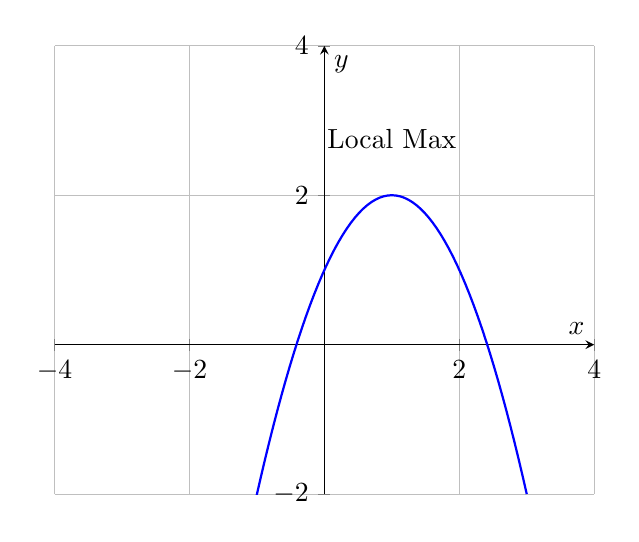
\begin{tikzpicture}
\begin{axis}[xmin=-4, xmax=4, ymin=-2, ymax=4, axis lines=center, xlabel=$x$, ylabel=$y$, samples=100, domain=-3:3, grid=both]
    \addplot[blue, thick] {-(x-1)^2 + 2};
    \node at (axis cs:1,2.5) [above] {Local Max};
\end{axis}
\end{tikzpicture}
\end{center}
}
} {}{NOTAGS}

 \ex
{\code{FxPROPx25x01x24x005}}{30}
{
Draw a graph with an absolute maximum, but no absolute minimum, which
does have a relative minimum.
}
{

 

\begin{center}
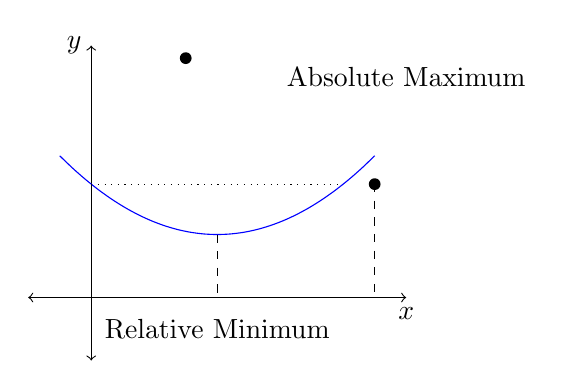
\begin{tikzpicture}[scale=0.8]
    \draw[<->] (-1,0) -- (5,0) node[below] {$x$};
    \draw[<->] (0,-1) -- (0,4) node[left] {$y$};
    \draw[domain=-0.5:4.5,smooth,variable=\x,blue] plot ({\x},{0.2*(\x-2)^2 + 1});
    \node at (2,-0.5) {\text{Relative Minimum}};
    \draw[dashed] (2,1) -- (2,0);
    \draw[dotted] (0,1.8) -- (4,1.8);
    \node at (5,3.5) {\text{Absolute Maximum}};
    \draw[dashed] (4.5,1.8) -- (4.5,0);
    % Dots
    \node at (1.5,3.8) [circle,fill,inner sep=1.5pt]{};
    \node at (4.5,1.8) [circle,fill,inner sep=1.5pt]{};
\end{tikzpicture}
\end{center}
} {}{NOTAGS}


 \ex
{\code{FxPROPx25x01x24x006}}{30}
{
Draw a graph of a function $f(x)$ with no absolute maximum, but such that
$|f(x) | < 10$. 
}
{

 

\begin{center}
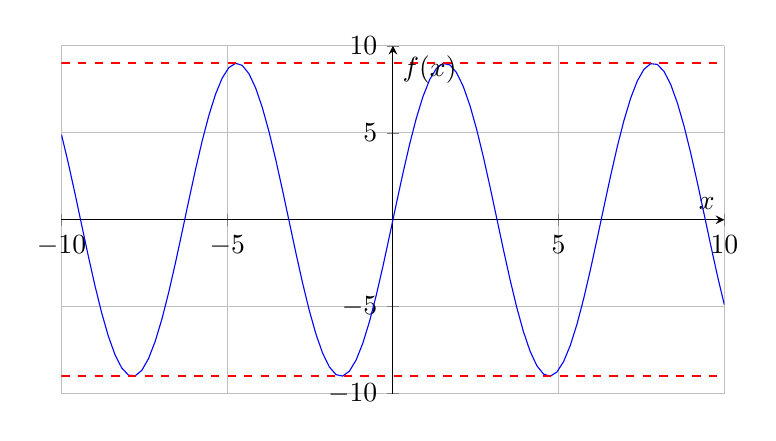
\begin{tikzpicture}
    \begin{axis}[
        axis lines=middle,
        xmin=-10, xmax=10,
        ymin=-10, ymax=10,
        xlabel={$x$},
        ylabel={$f(x)$},
        xtick={-10,-5,0,5,10},
        ytick={-10,-5,0,5,10},
        grid=both,
        width=10cm,
        height=6cm,
        domain=-10:10
    ]
    \addplot[blue, samples=100] {9*sin(deg(x))};
    \addplot[red, dashed, thick] coordinates {(-10,9) (10,9)};
    \addplot[red, dashed, thick] coordinates {(-10,-9) (10,-9)};
    \end{axis}
\end{tikzpicture}
\end{center}
} {}{NOTAGS}


 \ex
{\code{FxPROPx25x01x24x007}}{15}
{
For $h(x) = 5 \sqrt{x}$ what are its absolute extrema?
}
{

 

To find the absolute extrema of the function \( h(x) = 5 \sqrt{x} \), we need to consider the domain of the function, which is \( x \geq 0 \).

1. **Endpoints**: Evaluate the function at the endpoint \( x = 0 \).

   \[
   h(0) = 5 \sqrt{0} = 0
   \]

2. **Critical Points**: Find \( h'(x) \) and set it to zero to find any critical points.

   \[
   h(x) = 5x^{1/2} \implies h'(x) = \frac{5}{2} x^{-1/2} = \frac{5}{2\sqrt{x}}
   \]

   Since \( h'(x) \) is undefined at \( x = 0 \), we consider only \( x > 0 \) for critical points. \( h'(x) \) does not equal zero for any \( x > 0 \).

3. **Behavior at Infinity**: As \( x \to \infty \), \( h(x) = 5 \sqrt{x} \to \infty \).

The minimum occurs at the endpoint \( x = 0 \) with \( h(x) = 0 \). There is no maximum value since the function increases without bound as \( x \to \infty \).

**Conclusion**:

- Absolute minimum: \( h(x) = 0 \) at \( x = 0 \).
- No absolute maximum.
} {}{NOTAGS}


 \ex
{\code{FxPROPx25x01x24x008}}{15}
{
What are the absolute extrema of the graph of $y = x^2 + 1$?
}
{

 

The function \( y = x^2 + 1 \) is a parabola that opens upwards. Since it is defined for all real numbers and is continuous over its domain, we look for critical points by finding its derivative and setting it equal to zero.

The derivative is:

\[
y' = \frac{d}{dx}(x^2 + 1) = 2x
\]

Setting \( y' = 0 \):

\[
2x = 0 \implies x = 0
\]

Evaluating \( y \) at \( x = 0 \):

\[
y(0) = 0^2 + 1 = 1
\]

Since the parabola opens upwards and extends infinitely, the minimum value (absolute minimum) occurs at \( x = 0 \) and is \( y = 1 \). There is no absolute maximum because as \( x \to \pm \infty \), \( y \to \infty \).

Therefore, the absolute minimum is at \( (0, 1) \), and there is no absolute maximum.
} {}{NOTAGS}


 \ex
{\code{FxPROPx25x01x24x009}}{15}
{
What are the absolute extrema of the graph of $y = -3x^2 + 1$?
}
{

 

The function \( y = -3x^2 + 1 \) is a downward-opening parabola. To find the absolute extrema, we need to determine its vertex, as it represents the highest point for this particular quadratic function.

The vertex form of a parabola is given by:

\[ y = a(x-h)^2 + k \]

For the standard form \( y = ax^2 + bx + c \), the vertex \( (h, k) \) can be found using:

\[ h = -\frac{b}{2a} \]

Since here \( a = -3 \), \( b = 0 \), and \( c = 1 \), we calculate \( h \):

\[ h = -\frac{0}{2(-3)} = 0 \]

Therefore, the x-coordinate of the vertex is \( x = 0 \).

Substituting \( x = 0 \) back into the function to find the maximum value:

\[ y = -3(0)^2 + 1 = 1 \]

Thus, the vertex is \( (0, 1) \).

For a function \( y = -3x^2 + 1 \) open downwards, the vertex is the absolute maximum.

Therefore, the absolute maximum value of the function is:

\[ \boxed{1} \]

The function has no absolute minimum as it extends indefinitely downwards.
} {}{NOTAGS}




 \ex
{\code{TESTxFxPROPx25x02x14x001}}{15}
{
What are the absolute extrema of the graph of $y = (x-2)^2 + 1$?
(give the $x$ and $y$ coordinates)
}
{

 

The function \( y = (x-2)^2 + 1 \) is a parabola that opens upwards.

The vertex form of a quadratic function is \( y = a(x-h)^2 + k \), where \((h, k)\) is the vertex. For this function, the vertex is at \((2, 1)\).

Since the parabola opens upwards, the vertex represents the absolute minimum point, and there are no absolute maximum points as the graph extends to infinity in the positive \( y \)-direction.

Therefore, the absolute minimum occurs at:

\((x, y) = (2, 1)\)
} {}{type:TEST}


 \ex
{\code{FxPROPx25x09x15x001}}{15}
{
What are the absolute extrema of the graph of $y = (x+3)^2 -1$?
(give the $x$ and $y$ coordinates)
}
{

 

The function \( y = (x+3)^2 - 1 \) is a parabola that opens upward. 

To find the vertex, rewrite the function as \( y = (x+3)^2 - 1 \).

The vertex form of a parabola is \( y = a(x-h)^2 + k \), where \((h, k)\) is the vertex.

Here, \( a = 1 \), \( h = -3 \), and \( k = -1 \).

The vertex is \((-3, -1)\), which is the minimum point of the parabola.

Since the parabola opens upwards, \((-3, -1)\) is the absolute minimum.

There are no absolute maximum points since the parabola extends indefinitely upward.

Absolute minimum: \( (-3, -1) \) 

Absolute maximum: None
} {}{type:TEST}



 \ex
{\code{TESTxFxPROPx25x02x14x002}}{15}
{
Consider the function $f(x) = |x - 3|$.

\begin{enumerate}

\item On what intervals is $f$ increasing? On what intervals is $f$ decreasing?

\item
What are the local max/min of $f$? (give the $x$ and $y$ coordinate, and indicate if it is a max or min).

\end{enumerate}

}
{

 

$f(x) = |x - 3|$

\begin{enumerate}

\item 
The function $f(x)$ is decreasing on the interval $(-\infty, 3)$ and increasing on the interval $(3, \infty)$.

\item
The function $f$ has a local minimum at $(3, 0)$. There is no local maximum.

\end{enumerate}
} {}{ type:TEST }




\ex
{\code{GPTx26x02x20x005}}{10}
{
Consider the function $f$ given by the following table.

\begin{tabular}{l| l| l| l| l| l|}
$x$ & -4 & -2 & 0 & 3 & 6 \\
\hline
$f(x)$ & 10 & 8 & 5 & 1 & -2 \\
\hline
\end{tabular}

\begin{enumerate}
\item Evaluate $f(0)$.
\item Evaluate $f(-4)$.
\item For what $x$ does $f(x)=1$?
\item Is the function increasing or decreasing?
\end{enumerate}}
{

 

(1) $f(0)=5$.

(2) $f(-4)=10$.

(3) $f(x)=1$ when $x=3$.

(4) Outputs decrease as $x$ increases $\rightarrow$ decreasing function.
}{}{type: TEST}





\subsection{Basic Function Evaluation \topic{E}} 
 
 
 
 \ex
{\code{FxEx25x01x15x001}}{10}
{
Let $f(x) = 5x - 2$. Evaluate $f(2)$ and $f(0)$.
} {

 

$f(2) = 5(2) - 2 = 10 - 2 = 8$

$f(0) = 5(0) - 2 = 0 - 2 = -2$
} {}{NOTAGS} 
 
 
 
 \ex
{\code{FxEx25x01x15x002}}{10}
{
Let $f(t) = 10 - 5t$. Evaluate $f(2)$ and $f(0)$.
} {

 

$f(2) = 10 - 5(2) = 10 - 10 = 0$

$f(0) = 10 - 5(0) = 10 - 0 = 10$
} {}{NOTAGS} 
 
 
 
 \ex
{\code{FxEx25x01x15x003}}{15}
{
Let $g(x) = 4 + 3x^2$. Evaluate $g(2)$ and $g(-2)$.
} {

 

\(g(2) = 4 + 3(2)^2 = 4 + 3 \times 4 = 4 + 12 = 16\)

\(g(-2) = 4 + 3(-2)^2 = 4 + 3 \times 4 = 4 + 12 = 16\)
} {}{NOTAGS} 
 
 
 
 \ex
{\code{FxEx25x01x15x004}}{10}
{
Let $h(x) = 5 + 2x^3$. Evaluate $h(2)$ and $h(-2)$.
} {

 

$h(2) = 5 + 2(2)^3 = 5 + 2 \cdot 8 = 5 + 16 = 21$

$h(-2) = 5 + 2(-2)^3 = 5 + 2(-8) = 5 - 16 = -11$
} {}{NOTAGS} 
 

 \ex
{\code{FxEx25x02x12x001}}{20}
{
Let $f(x) = 5x + 2x^2$. Evaluate $f(\frac{3}{2})$ and $f(-\frac{1}{2})$.
} {

SOLUTION:

\begin{itemize}

\item $f(\frac{3}{2}) = \hfill 5\cdot \frac{3}{2} + 2(\frac{3}{2})^2 = \hfill \frac{15}{2} +
2\cdot \frac{9}{4} = \hfill \frac{15}{2} + \frac{9}{2} = \frac{24}{2} = \hfill 12$

\vspace{5mm}

\item $f(-\frac{1}{2}) = \hfill 5\cdot -\frac{1}{2} + 2(-\frac{1}{2})^2 = 
\hfill \frac{-5}{2} + 2 \cdot \frac{1}{4} = \hfill \frac{-5}{2} + \frac{1}{2} = \hfill \frac{-4}{2} = \hfill -2$

\end{itemize}

} {}{NOTAGS} 
 
 

 

  
 
 
 \ex
{\code{FxEx25x01x15x005}}{10}
{
Let $h(u) = \dfrac{5 + u}{u - 5}$. Evaluate $h(0)$ and $h(-1)$.
} {

SOLUTION:
\begin{itemize}

\item
$h(0) = \ \ \ \ \dfrac{5 + 0}{0 - 5} \ \ \ \ = \ \ \ \ \dfrac{5}{-5} \ \ \ \ = \ \ \ \ -1$

\item
$h(-1) = \ \ \ \ \dfrac{5 + (-1)}{(-1) - 5} \ \ \ \ = \ \ \ \ \dfrac{4}{-6} \ \ \ \ = 
\ \ \ \ -\dfrac{2}{3}$

\end{itemize}

} {}{NOTAGS} 
 
 
 
 \ex
{\code{FxEx25x01x20x002}}{10}
{
 Let $h(x) = 13 + 5 \cdot (x - 2)^2$.
\begin{multicols}{2}
\begin{enumerate}
\item Evaluate $h(0)$.
\item Evaluate $h(2)$.
\end{enumerate}
\end{multicols}

} {

 

$h(0) = 13 + 5 \cdot (0 - 2)^2 = 13 + 5 \cdot 4 = 13 + 20 = 33$

$h(2) = 13 + 5 \cdot (2 - 2)^2 = 13 + 5 \cdot 0 = 13$
} {}{NOTAGS} 
 
 
 
 \ex
{\code{FxEx25x01x15x009}}{10}
{


Let $f(x) = 5x + 100$. Put the following values in order without evaluating:
$f(20), f(10), f(100)$. Explain.
} {

 

$f(x) = 5x + 100$

Since $f(x)$ is a linear function with a positive slope, it is an increasing function. Thus, the order of $f(x)$ values corresponds to the order of $x$ values.

Therefore, $f(10) < f(20) < f(100)$.
} {}{NOTAGS} 
 
 
 
 \ex
{\code{FxEx25x01x15x010}}{10}
{


Let $f(x) = -5x$. Put the following values in order without evaluating:
$f(20), f(10), f(100)$. Explain.
} {

 

$f(100), f(20), f(10)$

Since $f(x) = -5x$, as $x$ increases, $f(x)$ becomes more negative. Thus, $f(100) < f(20) < f(10)$.
} {}{NOTAGS} 
 
 
 
 \ex
{\code{FxEx25x01x15x011}}{10}
{


Let $f(x) = 5x - 10$. For what $x$ is the function value positive?
} {

 

The function $f(x) = 5x - 10$ is positive when:

\[
5x - 10 > 0
\]

Solving for $x$:

\[
5x > 10
\]

\[
x > 2
\]

Thus, the function value is positive for $x > 2$.
} {}{NOTAGS} 
 
 
 
 \ex
{\code{FxEx25x01x15x012}}{10}
{


Let $f(t) = 10 - 5t$. For what $t$ is the function value negative?
} {

 

To find for what values of \( t \) the function \( f(t) = 10 - 5t \) is negative, we solve the inequality:

\[ 
10 - 5t < 0 
\]

Subtract 10 from both sides:

\[ 
-5t < -10 
\]

Divide both sides by \(-5\):

\[ 
t > 2 
\]

Thus, the function value is negative for \( t > 2 \).
} {}{NOTAGS} 
 
 
 
 \ex
{\code{FxEx25x01x15x013}}{10}
{


Let $g(x) = 4 + 3x^2$. Are $g(20242024)$ and $g(-20242024)$ equal? Why?
} {

 

$g(20242024) = 4 + 3(20242024)^2$

$g(-20242024) = 4 + 3(-20242024)^2$

Since $(-20242024)^2 = (20242024)^2$, it follows that:

$g(20242024) = g(-20242024)$

Thus, $g(20242024)$ and $g(-20242024)$ are equal because the function $g(x)$ is based on $x^2$, which is the same for $x$ and $-x$.
} {}{NOTAGS} 
 
 
 
 \ex
{\code{FxEx25x01x15x014}}{10}
{


Let $h(x) = 5 + 2x^3$. Are $h(20242024)$ and $h(-20242024)$ equal? Why?
}
{

 

$h(x) = 5 + 2x^3$

For $h(20242024)$:

$h(20242024) = 5 + 2(20242024)^3$

For $h(-20242024)$:

$h(-20242024) = 5 + 2(-20242024)^3 = 5 - 2(20242024)^3$

Since $2(20242024)^3 \neq -2(20242024)^3$, $h(20242024) \neq h(-20242024)$.

Thus, $h(20242024)$ and $h(-20242024)$ are not equal.
} {}{NOTAGS}


 \ex
{\code{FxEx25x02x05x001}}{10}
{
Consider the piecewise defined function given by $f(x) =
\begin{cases}
x & if \ x<-2 \\
2x - 1 & if \ -2\le x\le 3 \\
-4x & if \ x > 3
\end{cases}
$

Find the following values.
\begin{multicols}{2}
\begin{enumerate}

\item $f(-5)= $

\item
$f(-2)= $
 
\item
$f(0)= $

\item
$f(3)= $ 

\item
$f(4)= $


\end{enumerate}
\end{multicols}

}
{

 

$f(-5) = -5$

$f(-2) = 2(-2) - 1 = -5$

$f(0) = 2(0) - 1 = -1$

$f(3) = 2(3) - 1 = 5$

$f(4) = -4(4) = -16$
} {}{NOTAGS}


 \ex
{\code{TESTxFxEx25x02x12x101}}{15}
{
Let $h(x) = x^4 - 2x^3$. Evaluate $h(2)$ and $h(-2)$.
} {

 

$h(2) = 2^4 - 2(2)^3 = 16 - 16 = 0$

$h(-2) = (-2)^4 - 2(-2)^3 = 16 + 16 = 32$
} {}{NOTAGS} 


 \ex
{\code{FxEx25x09x15x002}}{15}
{
Let $g(x) = 3x^3 - x^4$. Evaluate $g(2)$ and $g(-2)$.
} {

SOLUTION:

$g(2) = 3(2)^3 - (2)^4 = 3 \cdot 8 - 16 = 8$

$g(-2) = 3(-2)^3 - (-2)^4 = 3 \cdot (-8) - 16 = -40$

} {}{type: TEST} 


\ex
{\code{GPTx26x02x20x003}}{25}
{
Let $g(x) = 2x^3 - x^4$. Evaluate $g(1)$ and $g(-1)$.
}
{

 

$g(1) = 2(1)^3 - (1)^4 = 2 - 1 = 1$.

$g(-1) = 2(-1)^3 - (-1)^4 = -2 - 1 = -3$.
} {}{type: TEST}




 \ex
{\code{TESTxFxEx25x02x12x002}}{25}
{
Evaluate $f(0)$, $f(4)$, and $f(5)$ where 
$f(x) =
\begin{cases}
x^2 & if \ x<5 \\
5-x & if \ x \ge 5
\end{cases}
$

Also, is $f$ a one-to-one function?

}
{

 

$f(0) = 
\begin{cases} 
0^2 = 0 & \text{if } 0 < 5 
\end{cases}
$

$f(4) = 
\begin{cases} 
4^2 = 16 & \text{if } 4 < 5 
\end{cases}
$

$f(5) = 
\begin{cases} 
5-5 = 0 & \text{if } 5 \ge 5 
\end{cases}
$

To determine if $f$ is one-to-one, observe that:

For $x < 5$, $f(x) = x^2$. This part is not one-to-one as different $x$ values can give the same $f(x)$ (e.g., $f(-2) = 4$ and $f(2) = 4$).

For $x \ge 5$, $f(x) = 5 - x$. This part is one-to-one since if $f(x_1) = f(x_2)$, then $5 - x_1 = 5 - x_2$, which leads to $x_1 = x_2$.

However, combining these intervals, $f$ fails to be one-to-one since $f(2) = 4$ and $f(-2) = 4$. 

Therefore, $f$ is not a one-to-one function.
} {}{NOTAGS}


 \ex
{\code{FxEx25x09x15x004}}{25}
{
Evaluate $f(0)$, $f(3)$, and $f(4)$ where 
$f(x) =
\begin{cases}
x^2 & if \ x \le 3 \\
10 + x & if \ x > 3
\end{cases}
$

Also, is $f$ a one-to-one function?

}
{

SOLUTION:

$f(0) = (0)^2 = 0$ (since $0 \le 3$)

$f(3) = (3)^2 = 9$ (since $3 \le 3$)

$f(4) = 10 + (4) = 14$ (since $4 > 3$)

No, the function is NOT one-to-one since $f(2) = f(-2) = 4$,
that is we repeat the output 4 (or think: two different inputs have the same output).

} {}{type: TEST}
 

 \ex
{\code{GROUPxFxEx25x02x07x001}}{50}
{

 The horizon is the line where the earth and sky meet.  Your distance from the horizon depends on your height above sea level.  The function
$f(h) = \sqrt{2h}$ gives the distance to the horizon (in miles), where $h$ is your height (in feet) above sea level.

\vspace{5mm}

\noindent
Suppose your group went to the beach and you are standing right at sea level with your feet in the water. The distance of the horizon from your gaze will depend on your height.  
For each person in your group, determine how far away the horizon appears to be
(note: find your height in feet; for example a kid that is 3 feet 6 inches tall is 3.5 feet tall).


}
{

 

$f(h) = \sqrt{2h}$

For a person with height $h$ feet:

1. Calculate the distance to the horizon in miles using the height $h$.
2. Example: If $h = 3.5$ feet (a child who is 3 feet 6 inches tall), then:

   \[
   f(3.5) = \sqrt{2 \times 3.5} = \sqrt{7} \approx 2.65 \text{ miles}
   \]

For each group member, substitute their height into $f(h)$ and calculate the distance using the formula.
} {}{NOTAGS}



\subsection{Function Evaluation From Table \topic{ETAB}} 
 

\ex
{\code{FxETABx25x01x23x001}}{5}
{
Consider the function \(f\) given by the following table. 
\begin{table}[H]
    \begin{tabular}{l| l| l| l| l| l|  l|}

     $x$  & $2$ 
           & $4$ 
           & $6$ 
           & $17$ 
           & $15$ 
           & $10$ 
\\
      \hline

     $f(x)$  & $-3$ 
               & $4$ 
               & $-13$ 
               & $2$ 
               & $0$ 
               & $14$
\\
      \hline
    \end{tabular}
\end{table}

\noindent

\begin{multicols}{2}
\begin{enumerate}
\item Evaluate \(f(17)\)
\item Evaluate \(f(2)\)

\item For what $x$ does $f(x) = -13$
\item Solve $f(x) = 6$.

\end{enumerate}
\end{multicols}
}
{

 

\begin{enumerate}
    \item \(f(17) = 2\)
    \item \(f(2) = -3\)
    \item \(f(x) = -13\) when \(x = 6\)
    \item There is no \(x\) such that \(f(x) = 6\)
\end{enumerate}
} {}{NOTAGS}


\ex
{\code{FxETABx25x01x23x002}}{5}
{
Consider the function \(f\) given by the following table. 
\begin{table}[H]
    \begin{tabular}{l| l| l| l| l| l|  l|}

     $x$  & $-4$ 
           & $4$ 
           & $0$ 
           & $17$ 
           & $5$ 
           & $10$ 
\\
      \hline

     $f(x)$  & $-3$ 
               & $4$ 
               & $-13$ 
               & $2$ 
               & $0$ 
               & $0$
\\
      \hline
    \end{tabular}
\end{table}

\noindent

\begin{multicols}{2}
\begin{enumerate}
\item Evaluate \(f(0)\)
\item Solve \(f(x) = 0\)

\item For what $x$ is $f(x)$ negative?
\item Which $x$ value is a ``fixed point'' of $f$?

\end{enumerate}
\end{multicols}
}
{

 

\( f(0) = -13 \)

To solve \( f(x) = 0 \), we look at the table and find the \( x \) values for which \( f(x) = 0 \). These are \( x = 5 \) and \( x = 10 \).

\( f(x) \) is negative for the \( x \) values where \( f(x) < 0 \). From the table, \( f(x) \) is negative at \( x = -4 \) and \( x = 0 \).

A fixed point occurs when \( f(x) = x \). From the table, there is no \( x \) such that \( f(x) = x \). Thus, there is no fixed point.
} {}{NOTAGS}



\ex
{\code{TESTxFxETABx25x02x12x001}}{5}
{
Consider the function \(f\) given by the following table. 
\begin{table}[H]
    \begin{tabular}{l| l| l| l| l| l|  l|}

     $x$  & $2$ 
           & $-3$ 
           & $6$ 
           & $1$ 
           & $0$ 
           & $-9$ 
\\
      \hline

     $f(x)$  & $0$ 
               & $1$ 
               & $-1$ 
               & $0$ 
               & $-3$ 
               & $9$
\\
      \hline
    \end{tabular}
\end{table}

\noindent

\begin{multicols}{2}
\begin{enumerate}
\item Evaluate \(f(0)\)
\item Evaluate \(f(-3)\)

\item For what $x$ does $f(x) = 0$

\end{enumerate}
\end{multicols}
}
{

 

\(f(0) = -3\)

\(f(-3) = 1\)

\(f(x) = 0\) for \(x = 2\) and \(x = 1\)
} {}{NOTAGS}



\ex
{\code{FxETABx25x09x15x001}}{10}
{
Consider the function \(f\) given by the following table. 
\begin{table}[H]
    \begin{tabular}{l| l| l| l| l| l|  l|}

     $x$  & $-3$ 
           & $-1$ 
           & $0$ 
           & $1$ 
           & $7$ 
           & $9$ 
\\
      \hline

     $f(x)$  & $9$ 
               & $7$ 
               & $6$ 
               & $0$ 
               & $-3$ 
               & $-5$
\\
      \hline
    \end{tabular}
\end{table}

\noindent

\begin{multicols}{2}
\begin{enumerate}
\item Evaluate \(f(0)\)
\item Evaluate \(f(-3)\)

\item For what $x$ does $f(x) = -1$

\item Is the function increasing or decreasing?

\end{enumerate}
\end{multicols}
}
{

SOLUTION:

a) $f(0) = 6$ \ and \ b) $f(-3) = 9$ \ and \ c) No $x$ values.

d) Decreasing, since as the input values go up from $-3$ to $9$, the corresponding output values go down from $9$ to $-5$.

} {}{type: TEST}


\subsection{Function Evaluation At Variable Input \topic{EVAR}} 
 
 
\ex
{\code{FxEVARx25x01x23x002}}{15}
{
Let $g(x) = 2x - 1$. Evaluate $g(y + 3)$. 
} {

 

\[ g(y + 3) = 2(y + 3) - 1 = 2y + 6 - 1 = 2y + 5 \]
} {}{NOTAGS}  
 
 
\ex
{\code{FxEVARx25x01x23x001}}{15}
{
Let $f(x) = 5 + 2x^3$. Evaluate $f(t)$ and $f(-u)$. 
} {

 

$f(t) = 5 + 2t^3$

$f(-u) = 5 + 2(-u)^3 = 5 - 2u^3$
} {}{NOTAGS} 


\ex
{\code{FxEVARx25x01x23x003}}{15}
{
Let $h(t) = t^2  - t$. Evaluate $h(-x)$ and $h(x - 1)$. 
} {

 

$h(-x) = (-x)^2 - (-x) = x^2 + x$

$h(x-1) = (x-1)^2 - (x-1) = x^2 - 2x + 1 - x + 1 = x^2 - 3x + 2$
} {}{NOTAGS}  
 
 
\ex
{\code{FxEVARx25x02x03x003}}{15}
{
For the function $f(x) = \dfrac{3 x^2 -1}{x^2}$, 
find (and simplify when possible)\medskip

\begin{multicols}{2}
\begin {enumerate}
\item
$f(2)= $

\item 
$f(-1)= $

\item
$f(r)= $

\item
$f(x-1)= $

\item
$f(-x)=$

\item
$f(x^3)= $
\end{enumerate}
\end{multicols}

} {$\frac{11}{4}, 2,  \frac{3 r^2 -1}{r^2}, \frac{3 (x-1)^2 -1}{(x-1)^2}=\frac{3x^2 -
6x + 2}{(x-1)^2}, \frac{3(-x)^2 -1}{(-x)^2}= \frac{3 x^2 -1}{x^2},
\frac{3 x^6 -1}{x^6}$} {}{NOTAGS}   
 



\ex
{\code{FxEVARx25x02x05x001}}{15}
{
Let $f(x)=x^2+x-2$ and $g(x) = \dfrac{x}{x^2+3}$. Find (and simplify) the following.

\begin{multicols}{2}
\begin {enumerate}

\item
$f(x+4)$

\item 
$f(x^2-1)$ 

\item
$g(x^2)$

\item
$g(u)$ 



\end{enumerate}
\end{multicols}

} {

 

$f(x+4) = (x+4)^2 + (x+4) - 2 = x^2 + 8x + 16 + x + 4 - 2 = x^2 + 9x + 18$

$f(x^2-1) = (x^2-1)^2 + (x^2-1) - 2 = x^4 - 2x^2 + 1 + x^2 - 1 - 2 = x^4 - x^2 - 2$

$g(x^2) = \dfrac{x^2}{(x^2)^2 + 3} = \dfrac{x^2}{x^4 + 3}$

$g(u) = \dfrac{u}{u^2 + 3}$
} {}{NOTAGS}   
 

 \ex
{\code{TESTxFxEVARx25x02x12x001}}{15}
{
Let $g(t) = 3t^2$. Evaluate $g(-x)$ and $g(x - 2)$. 
} {

 

$g(-x) = 3(-x)^2 = 3x^2$

$g(x-2) = 3(x-2)^2 = 3(x^2 - 4x + 4) = 3x^2 - 12x + 12$
} {}{NOTAGS}  


 \ex
{\code{FxEVARx25x09x15x001}}{15}
{
Let $h(t) = -4t$. Evaluate $h(-x)$ and $h(x - 2)$. 
} {

SOLUTION:

$h(-x) = -4(-x) = 4x$

$h(x-2) = -4(x-2) = -4x + 8$


} {}{type: TEST}  



\ex
{\code{GPTx26x02x20x006}}{30}
{
Let $h(t)=5t$. Evaluate $h(-x)$ and $h(x+3)$.
}
{

 

$h(-x)=5(-x)=-5x$.

$h(x+3)=5(x+3)=5x+15$.
} {}{type: TEST}
 


\subsection{One Variable as Function of Other Variable \topic{VAR}} 

 \ex
{\code{FxVARx25x01x23x001}}{10}
{
Consider the equation $30x = 10y$.  Write $y$ as a function of $x$.
}
{

 

The equation is given by:

\[ 30x = 10y \]

To express \( y \) as a function of \( x \), divide both sides by 10:

\[ y = \frac{30x}{10} \]

Simplifying gives:

\[ y = 3x \]
} {}{NOTAGS}


 \ex
{\code{FxVARx25x01x23x002}}{10}
{
Consider the equation $6x = 8y$.  Write $x$ as a function of $y$.
}
{

 

\( x = \frac{4}{3}y \)
} {}{NOTAGS}

 \ex
{\code{FxVARx25x01x23x003}}{10}
{
Consider the equation $6t = 8y + 4$.  Write $y$ as a function of $t$.
}
{

 

$6t = 8y + 4$

Subtract 4 from both sides:

$6t - 4 = 8y$

Divide both sides by 8 to solve for $y$:

$y = \frac{6t - 4}{8}$

Simplify:

$y = \frac{3t - 2}{4}$

Thus, $y$ as a function of $t$ is:

$y(t) = \frac{3t - 2}{4}$
} {}{NOTAGS}

 \ex
{\code{FxVARx25x01x23x004}}{15}
{
Consider the equation $u  = 3u + 8x^3 - 4$.  Write $u$ as a function of $x$.
}
{

 

\( u - 3u = 8x^3 - 4 \)

\( -2u = 8x^3 - 4 \)

\( u = -\frac{1}{2}(8x^3 - 4) \)

\( u = -4x^3 + 2 \)

So, \( u(x) = -4x^3 + 2 \).
} {}{NOTAGS}

%BREAK
\end{itemize}
\begin{itemize}

\subsection{Evaluation and Simplifying for Log/Exp \topic{ELE}}  
 
 
 
 \ex
{\code{FxELEx25x01x20x010}}{10}
{
 Evaluate the following expressions:

\begin{enumerate}
\item \(\log_2(16)\)
\item \(\log_2\bigl(\tfrac{1}{16}\bigr)\)
\end{enumerate}
} {

 

\(\log_2(16) = \log_2(2^4) = 4\)

\(\log_2\bigl(\tfrac{1}{16}\bigr) = \log_2(16^{-1}) = -\log_2(16) = -4\)
} {}{NOTAGS} 
 
 
 
 \ex
{\code{FxELEx25x01x20x011}}{10}
{
  Evaluate the following expressions:

\begin{enumerate}
\item \(\log_{2018}(1)\)
\item \(\log_{2018}(0)\)
\end{enumerate}
} {

 

\(\log_{2018}(1) = 0\)

\(\log_{2018}(0) \text{ is undefined because the logarithm of zero is undefined.}\)
} {}{NOTAGS} 
 
 
 
 \ex
{\code{FxELEx25x01x20x012}}{10}
{
 Evaluate the following expressions:

\begin{enumerate}
\item \(\log_{17}(17^{899})\)
\item \(13^{\log_{13}(255)}\)
\end{enumerate}
} {

 

\(\log_{17}(17^{899}) = 899\)

\(13^{\log_{13}(255)} = 255\)
} {}{NOTAGS} 
 
 
 
 \ex
{\code{FxELEx25x01x20x013}}{10}
{
  Evaluate the following expression (be careful!):

\(\log_2\bigl(4^2\bigr)\) 

} {

 

\(\log_2\bigl(4^2\bigr) = \log_2(16) = 4\)
} {}{NOTAGS} 
 
 
 
 \ex
{\code{FxELEx25x01x20x008}}{10}
{
 Evaluate/simplify or state if undefined (and why):

\(\log_{\frac12}\bigl(\tfrac{1}{2}\bigr)\)


} {

 

\(\log_{\frac{1}{2}}\Bigl(\frac{1}{2}\Bigr) = 1\)
} {}{NOTAGS} 
 
 
 
 \ex
{\code{FxELEx25x01x20x009}}{10}
{
Simplify.
\begin{enumerate}
\item \(\log_{\frac12}(8)\)
\item \(\log_{38}(1)\)
\end{enumerate}

} {

 

\(\log_{\frac12}(8) = \log_{\frac12}\left(\frac{1}{\frac{1}{8}}\right) = -\log_{\frac12}\left(\frac{1}{8}\right) = -\left(\log_{2}(8) \cdot \log_{\frac12}(2)\right) = -\left(3 \cdot (-1)\right) = 3\)

\(\log_{38}(1) = 0\)
} {}{NOTAGS} 
 
 
 
 \ex
{\code{FxELEx25x01x20x110}}{10}
{
Simplify.
\begin{enumerate}
\item \(\log_{38}(0)\)
\item \(\log_{x}(x^{89})\)
\end{enumerate}

} {

 

\(\log_{38}(0)\) is undefined because \(\log_{b}(0)\) is undefined for any base \(b\).

\(\log_{x}(x^{89}) = 89\) because \(\log_{b}(b^k) = k\).
} {}{NOTAGS} 
 
 
 
 \ex
{\code{FxELEx25x01x20x111}}{10}
{

Simplify. \(15^{\log_{15}(3y + 7)}\)

} {

 

\(15^{\log_{15}(3y + 7)} = 3y + 7\)
} {}{NOTAGS} 
 
 
 
 \ex
{\code{FxELEx25x01x20x112}}{10}
{
Simplify $\log_{\frac12}\bigl(\tfrac{1}{16}\bigr)$

} {

 

\[
\log_{\frac{1}{2}}\left(\frac{1}{16}\right) = \log_{\frac{1}{2}}\left(\left(\frac{1}{2}\right)^4\right) = 4 \cdot \log_{\frac{1}{2}}\left(\frac{1}{2}\right) = 4 \cdot (-1) = -4
\]
} {}{NOTAGS} 
 
 
 \ex
{\code{FxELEx25x01x22x006}}{10}
{
Simplify each expression:
\begin{multicols}{2}
\begin{enumerate}
\item \(\ln(e^{3x})\)
\item \(\log_2\!\bigl(\tfrac{1}{4}\bigr)\)
\end{enumerate}
\end{multicols}
\begin{enumerate}
\item \(4^{\log_4(x-9)}\)
\end{enumerate}
}{

 

\(\ln(e^{3x}) = 3x\)

\(\log_2\!\bigl(\tfrac{1}{4}\bigr) = -2\)

\(4^{\log_4(x-9)} = x-9\)
}{}{NOTAGS}



 \ex
{\code{FxELEx25x02x04x001}}{10}
{
Simplify each expression:
\begin{multicols}{2}
\begin{enumerate}
\item $\log_3\frac{1}{3}$

\item $\log_6\sqrt{6}$
\end{enumerate}
\end{multicols}

}{

 

$\log_3\frac{1}{3} = \log_3 3^{-1} = -1$

$\log_6\sqrt{6} = \log_6 6^{\frac{1}{2}} = \frac{1}{2}$
}{}{NOTAGS}

 
 
 \ex
{\code{FxELEx25x01x20x027}}{10}
{
Let \(f(x) = x^{\tfrac{5}{3}}\) and \(g(x) = x^{\tfrac{5}{2}}\).

Which is larger, \(f(2018)\) or \(g(2018)\)? Justify without a calculator.

}
{

 

To compare \(f(2018)\) and \(g(2018)\), we consider the functions \(f(x) = x^{\tfrac{5}{3}}\) and \(g(x) = x^{\tfrac{5}{2}}\).

Observe that:

1. For \(x > 0\), both functions \(f(x)\) and \(g(x)\) are increasing functions since both have positive exponents.

2. Notice that \(\tfrac{5}{2} > \tfrac{5}{3}\), meaning the exponent for \(g(x)\) is larger than that for \(f(x)\).

This implies that, given the same \(x > 0\), \(g(x)\) grows faster than \(f(x)\).

Thus, for any positive value of \(x\), we have:

\[ g(x) = x^{\tfrac{5}{2}} > x^{\tfrac{5}{3}} = f(x). \]

Therefore, specifically for \(x = 2018\), it follows that:

\[ g(2018) > f(2018). \]
} {}{NOTAGS}


 \ex
{\code{TESTxxxFxELEx25x04x28x001}}{20}
{
Evaluate.
\begin{multicols}{3}
\begin{enumerate}

\item $\log_{17} (1)$

\item \(\log_{4}(16)\)

\item \(\log_{3}(\frac{1}{27})\)
\end{enumerate}
\end{multicols}

} {

SOLUTION:

\vspace{3mm}

a) $\log_{17} (1) = 0$ (since $17^0 = 1$)

\vspace{5mm}

b) $\log_{4}(16) = x$ converted to exponential equation: $4^x = 16$, so value is: 2.

\vspace{5mm}

c) $\log_{3}(\frac{1}{27}) = x$  converted to exponential equation: $3^x = \frac{1}{27}$, so value is: -3.

} {}{NOTAGS} 


 \ex
{\code{FxELEx25x11x17x001}}{20}
{
Evaluate each expression or state why it is undefined.
\begin{multicols}{3}
\begin{enumerate}

\item $\log_{15} (1)$

\item \(\log_{15}(-1)\)

\item \(\log_{19}(\frac{1}{19})\)
\end{enumerate}
\end{multicols}

} {

SOLUTION:

\vspace{3mm}

a) $\log_{15} (1) = 0$ (since $15^0 = 1$)

\vspace{5mm}

b) $\log_{15}(-1)$ is undefined since the domain of $\log$ is positive reals, so
it is not defined at $-1$.

\vspace{5mm}

c) $\log_{19}(\frac{1}{19}) = x$  converted to exponential equation: $19^x = \frac{1}{19}$, so value is: -1.

} {}{type: TEST} 



\subsection{Log Properties \topic{LP}}  




\ex
{\code{FxLPx25x02x04x001}}{15}
{
Evaluate
\begin{multicols}{2}
\begin{enumerate}
\item $\log_{102} 102^4$

\item $\log_3 (\log_8 2)$
\end{enumerate}
\end{multicols}
}{

 

\(\log_{102} 102^4 = 4\)

To evaluate \(\log_3 (\log_8 2)\), first find \(\log_8 2\):

\[
\log_8 2 = \frac{\log_2 2}{\log_2 8} = \frac{1}{3}
\]

Then evaluate \(\log_3 \left( \frac{1}{3} \right)\):

\[
\log_3 \left( \frac{1}{3} \right) = -1
\]

So, \(\log_3 (\log_8 2) = -1\)
}{}{NOTAGS}





\ex
{\code{FxLPx25x02x04x003}}{15}
{
Simplify.
\begin{multicols}{2}
\begin{enumerate}
\item
$\log_a a^{\frac{1}{5}}$ 
\item
$\log_a {\sqrt[3]{a}}$



\end{enumerate}
\end{multicols}
}{

 

$\log_a a^{\frac{1}{5}} = \frac{1}{5} \log_a a = \frac{1}{5}$

$\log_a \sqrt[3]{a} = \log_a a^{\frac{1}{3}} = \frac{1}{3} \log_a a = \frac{1}{3}$
}{}{NOTAGS}

\ex
{\code{FxLPx25x02x04x004}}{15}
{
Simplify.
\begin{multicols}{2}
\begin{enumerate}
\item
$2^{\log_2 7}$ 
\item
$a^{\log_{a}{1\over 5}}$ 



\end{enumerate}
\end{multicols}
}{

 

$2^{\log_2 7} = 7$

$a^{\log_{a}\frac{1}{5}} = \frac{1}{5}$
}{}{NOTAGS}

\ex
{\code{FxLPx25x02x04x005}}{15}
{
Simplify.
\begin{multicols}{2}
\begin{enumerate}
\item
$10^{\log \sqrt{4}}$ 
\item
$e^{\ln 3 x^2}$

\end{enumerate}
\end{multicols}
}{

 

$10^{\log \sqrt{4}} = 10^{\log 2} = 2$

$e^{\ln 3 x^2} = 3x^2$
}{}{NOTAGS}







\ex
{\code{FxLPx25x02x04x006}}{20}
{
Use the properties of logarithms to expand the following
expressions.
\begin{multicols}{2}
\begin{enumerate}

\item
$\log_9 (5y)= $
\item
$\log_8 x^7 = $


\end{enumerate}
\end{multicols}
}{SOLUTION: $\log_9 5 +  \log_9 y  \ \ \ \hbox{ and } \ \ \ 7\log_8 x$}{}{NOTAGS}


\ex
{\code{FxLPx25x02x04x007}}{20}
{
Use the properties of logarithms to expand the following
expressions.
\begin{multicols}{2}
\begin{enumerate}

\item
$\log_b (3x^2y^3)$
\item
$\log_8\dfrac{x^{  \frac{1}{2}  }}{y^3}$ 

\end{enumerate}
\end{multicols}
}{

 

\(\log_b (3x^2y^3) = \log_b 3 + \log_b x^2 + \log_b y^3 = \log_b 3 + 2\log_b x + 3\log_b y\)

\(\log_8 \dfrac{x^{\frac{1}{2}}}{y^3} = \log_8 x^{\frac{1}{2}} - \log_8 y^3 = \frac{1}{2}\log_8 x - 3\log_8 y\)
}{}{NOTAGS}


\ex
{\code{FxLPx25x02x04x008}}{20}
{
Use the properties of logarithms to expand the following
expressions.
\begin{multicols}{2}
\begin{enumerate}

\item
$\log_5 \sqrt[5]{ \dfrac{ x^2 }{y} } $
\item 
$\ln \left[\dfrac{x^4\sqrt{x^2+3}}{(x+3)^5}\right]$

\end{enumerate}
\end{multicols}
}{

 

$\log_5 \sqrt[5]{ \dfrac{ x^2 }{y} } = \log_5 \left( \dfrac{ x^2 }{y} \right)^{1/5} = \frac{1}{5} \log_5 \left( \dfrac{ x^2 }{y} \right) = \frac{1}{5} \left( \log_5 x^2 - \log_5 y \right) = \frac{2}{5} \log_5 x - \frac{1}{5} \log_5 y$

$\ln \left[\dfrac{x^4\sqrt{x^2+3}}{(x+3)^5}\right] = \ln \left( x^4\sqrt{x^2+3} \right) - \ln \left( (x+3)^5 \right) = \ln x^4 + \ln (x^2+3)^{1/2} - 5\ln(x+3) = 4\ln x + \frac{1}{2} \ln (x^2+3) - 5\ln(x+3)$
}{}{NOTAGS}







\ex
{\code{FxLPx25x02x04x009}}{20}
{
Use the properties of logarithms to condense the following
expressions.
\begin{multicols}{2}
\begin{enumerate}

\item
$\log x+\log 5= $ 
\item
$\log_8 x + 3 \log_8 y= $

\end{enumerate}
\end{multicols}
}{

 

\(\log x+\log 5 = \log(5x)\)

\(\log_8 x + 3 \log_8 y = \log_8 (x y^3)\)
}{}{NOTAGS}



\ex
{\code{FxLPx25x02x04x011}}{20}
{
Use the properties of logarithms to condense the following
expressions.
\begin{multicols}{2}
\begin{enumerate}

\item
$\frac{1}{2}(\log x+\log y)=$ 
\item
$\frac{1}{3}(\log_7 x + 4 \log_7 y) - 3 \log_7 (x+y)=$

\end{enumerate}
\end{multicols}
}{ SOLUTION: $\log \sqrt{xy}  \ \ \ \hbox{ and }\ \ \   \log_7 
\dfrac{{ \sqrt[3]{x y^4}  }}{(x+y)^3}$}{}{NOTAGS}








 


\ex
{\code{FxLPx25x02x04x012}}{20}
{
Use the change of base formula to write the following logarithms
as logarithms in the indicated base.
\begin{multicols}{2}
\begin{enumerate}

\item
$\log_7 12$; write it in base $10$.

\item
$\log_9 127$; write it in base $e$.

\end{enumerate}
\end{multicols}
}{ SOLUTION: $\log_7 12 = \dfrac{\log 12}{\log 7}   \ \ \ 
\hbox{ and }\ \ \   \log_9 127 = \dfrac{\ln 127}{\ln 9}$}{}{NOTAGS}


\ex
{\code{FxLPx25x02x04x013}}{20}
{
Use the change of base formula to write the following logarithms
as logarithms in the indicated base.
\begin{multicols}{2}
\begin{enumerate}

\item
$\log_{25} 9$; write it in base $5$ and simplify.




\item
$\log_{ \frac{1}{2} } 8$; write it in base $2$ and simplify.




\end{enumerate}
\end{multicols}
}{ SOLUTION: 
$\log_{25} 9 = \dfrac{\log_5 9}{\log_{5} 25}
=\dfrac{\log_5 9}{2}$

$\log_{ \frac{1}{2} } 8 =  \dfrac{\log_2 8}{\log_2
{\textstyle \frac{1}{2}}} = \dfrac{3}{-1} = -3$}{}{NOTAGS}

\ex
{\code{TESTxFxLPx25x02x04x002}}{20}
{
Simplify.
\begin{multicols}{2}
\begin{enumerate}
\item
$\log_a a^4$ 
\item
$\log_a\frac{1}{a^7}$ 



\end{enumerate}
\end{multicols}
}{

SOLUTION:

\vspace{3mm}

a) $\log_a a^4 = 4 \log_a a = 4\cdot 1 = 4$

\vspace{5mm}


b) $\log_a\frac{1}{a^7} = \log_a a^{-7} = (-7) \cdot \log_a a = (-7)\cdot 1 = -7$ 

}{}{NOTAGS}


\ex
{\code{TESTxFxLPx25x01x22x010}}{40}
{
\begin{multicols}{2}
\begin{enumerate}
\item Condense \(3\log_{10}(A) + 4\log_{10}(B)\) into a single log.
\item Use log properties to expand \(\log_7\!\bigl(\tfrac{x^5}{y^2}\bigr)\).
\end{enumerate}
\end{multicols}
}{

SOLUTION:


\begin{enumerate}

\item
 $3\log_{10}(A) + 4\log_{10}(B) = \log_{10}(A^3) + \log_{10}(B^4) = \log_{10}(A^3B^4)$

\vspace{8mm}

\item \( \log_7\!\bigl(\tfrac{x^5}{y^2}\bigr) =   
\log_7 (x^5) - \log_7 (y^2)  = 5\log_7 (x) - 2\log_7 (y) \)

\end{enumerate}

}{}{NOTAGS}




\ex
{\code{FxLPx25x11x17x001}}{45}
{
\begin{multicols}{2}
\begin{enumerate}
\item Condense $3\log (a) + \log (c) - \log (a^2) $ into a single log and simplify.
\item Use log properties to expand \(\log_4\!\bigl(\tfrac{x}{yw}\bigr)\).
\end{enumerate}
\end{multicols}
}{

SOLUTION:


\begin{enumerate}

\item 
$
= \log (a^3) + \log (c) - \log (a^2)
= \log (a^3 \cdot c)  - \log (a^2)
= \log (\frac{a^3 \cdot c}{a^2})
= \log (a \cdot c)$

\vspace{8mm}

\item  \(
= \log_4 (x) - \log_4 (yw)
=  \log_4 (x) - (\log_4 (y) + \log_4 (w) )
= \log_4 (x) - \log_4 (y) - \log_4 (w) 
\)




\end{enumerate}

}{}{type: TEST}



\subsection{Function Evaluation for Piece-wise Defined \topic{PC}}  
 
 
 
 \ex
{\code{FxPCx25x01x20x014}}{5}
{
Let 
\[
f(x)=
\begin{cases}
x - 2, & x \le -1,\\
2x+1, & x > -1.
\end{cases}
\]
Evaluate the following.
\begin{enumerate}
\item $f(-2)$
\item $f(-1)$

\item $f(0)$
\end{enumerate}
}
{

 

\[
f(-2) = (-2) - 2 = -4
\]

\[
f(-1) = (-1) - 2 = -3
\]

\[
f(0) = 2(0) + 1 = 1
\]
} {}{NOTAGS}


 \ex
{\code{FxPCx25x01x24x001}}{5}
{
Let 
\[
f(x)=
\begin{cases}
x^2, & x < 5,\\
-x, & x \ge 5.
\end{cases}
\]
Evaluate the following.
\begin{enumerate}
\item $f(65)$
\item $f(-5)$

\item $f(5)$
\end{enumerate}
}
{

 

\[
f(65) = 
\begin{cases}
x^2, & 65 < 5,\\
-x, & 65 \ge 5.
\end{cases}
= -65
\]

\[
f(-5) = 
\begin{cases}
x^2, & -5 < 5,\\
-x, & -5 \ge 5.
\end{cases}
= (-5)^2 = 25
\]

\[
f(5) = 
\begin{cases}
x^2, & 5 < 5,\\
-x, & 5 \ge 5.
\end{cases}
= -5
\]
} {}{NOTAGS}


\subsection{Evaluation (Mixed) \topic{EM}}  
 
\ex
{\code{FxEMx25x01x22x009}}{10}
{
Evaluate the following:
\begin{multicols}{2}
\begin{enumerate}
\item \(5\,i\,(2\,i - 3)\)
\item \(25^{-\tfrac{1}{2}}\)
\end{enumerate}
\end{multicols}
\begin{enumerate}
\item \(\log_5(25)\)
\end{enumerate}
}{

 

\(5\,i\,(2\,i - 3) = 5\,i \times 2\,i - 5\,i \times 3 = 10\,i^2 - 15\,i = 10(-1) - 15\,i = -10 - 15\,i\)

\[25^{-\tfrac{1}{2}} = \frac{1}{\sqrt{25}} = \frac{1}{5}\]

\(\log_5(25) = \log_5(5^2) = 2\)
}{}{NOTAGS}


\subsection{Function Categorization \topic{C}} 
 
 
 
 \ex
{\code{FxCx25x01x20x002}}{10}
{
For each of the following functions, determine:
\begin{itemize}
\item Whether it is a polynomial function.
\item Whether it is a rational function.
\end{itemize}

\begin{enumerate}
\item \(f(u) = \dfrac{4u}{5u^7 - 87}\)
\item \(h(y) = \sqrt{y^3 + 5y + 1}\)
\end{enumerate}
} {

 

\(f(u) = \dfrac{4u}{5u^7 - 87}\)

\begin{itemize}
\item Not a polynomial function (because it involves a division).
\item A rational function (since it is a ratio of two polynomials).
\end{itemize}

\(h(y) = \sqrt{y^3 + 5y + 1}\)

\begin{itemize}
\item Not a polynomial function (because it involves a square root).
\item Not a rational function (because it involves a square root).
\end{itemize}
} {}{NOTAGS} 
 
 
 
 \ex
{\code{FxCx25x01x20x003}}{10}
{
  For each of the following functions, determine:
\begin{itemize}
\item Whether it is a polynomial function.
\item Whether it is a rational function.
\end{itemize}

\begin{enumerate}
\item \(g(x) = \dfrac{x}{7}\)
\item \(g(x) = \dfrac{7}{x}\)
\end{enumerate}
}
{

 

1. For \( g(x) = \dfrac{x}{7} \):

   - **Polynomial Function**: Yes, \( g(x) = \frac{1}{7}x \), which is a linear polynomial.
   - **Rational Function**: Yes, since it can be written as \(\frac{x}{7}\), it is a rational function.

2. For \( g(x) = \dfrac{7}{x} \):

   - **Polynomial Function**: No, because polynomials cannot have variables in the denominator.
   - **Rational Function**: Yes, since it is the ratio of two polynomials \( \frac{7}{x} \), it is a rational function.
} {}{NOTAGS}


\ex
{\code{FxCx25x01x22x007}}{10}
{

\begin{enumerate}
\item Is \(f(x)=13^x\) an exponential function? If so, find its base.
\item Is \(f(x)=1^x\) an exponential function? If so, find its base.

\item Is \(f(x)=(-\tfrac12)^x\) an exponential function? If so, find its base.
\end{enumerate}
}{

 

\begin{enumerate}
\item Yes, \(f(x) = 13^x\) is an exponential function. The base is 13.

\item No, \(f(x) = 1^x\) is not considered an exponential function since the base 1 does not result in variable growth or decay; \(1^x\) is always 1.

\item Yes, \(f(x) = \left(-\tfrac{1}{2}\right)^x\) can be considered an exponential function, but it is important to note that the base \(-\tfrac{1}{2}\) being negative makes it complex or undefined in many cases unless \(x\) is an integer.
\end{enumerate}
}{}{NOTAGS}


\subsection{Basic Function Graphing \topic{G}} 
 
 
 
 \ex
{\code{FxGx24x12x28x001}}{20}
{
Draw a graph which is NOT a function.  Why is it not a function?
} {

 

To illustrate a graph which is NOT a function, we can consider the example of a vertical line, such as the line \( x = 2 \). A graph is not a function if there exists at least one vertical line that intersects the graph at more than one point. The vertical line \( x = 2 \) itself serves as such a graph:

\[
\begin{tikzpicture}
    \draw[->] (-1,0) -- (4,0) node[right] {x};
    \draw[->] (0,-2) -- (0,2) node[above] {y};
    \draw[thick,blue] (2,-2) -- (2,2);
    \node at (2.2, 1.8) {x=2};
\end{tikzpicture}
\]

The line \( x = 2 \) is not a function because it fails the vertical line test; it does not associate each \( x \)-value in its domain with a unique \( y \)-value.
} {}{NOTAGS} 
 
 
 
 \ex
{\code{FxGx24x12x28x002}}{20}
{
Draw a graph which  IS a function.  Why is it a function?
} {

 

A graph is considered a function if each input maps to exactly one output. Here's an example using a simple linear function:

Consider the linear function \( f(x) = 2x + 1 \).

The graph of this function can be drawn by plotting a set of points that satisfy the equation \( y = 2x + 1 \). Each \( x \) value maps to one unique \( y \) value, fulfilling the definition of a function.

Here's an example graph of the function \( f(x) = 2x + 1 \):

\[
\begin{array}{c|c}
x & y \\
\hline
-2 & -3 \\
-1 & -1 \\
0 & 1 \\
1 & 3 \\
2 & 5 \\
\end{array}
\]

The plot of these points on a coordinate plane results in a straight line, illustrating that it is a function because each vertical line intersects the graph in exactly one place.
} {}{NOTAGS} 
 
 
 
 \ex
{\code{FxGx24x12x28x102}}{20}
{
Draw a graph which is a one-to-one function.  Why is it a one-to-one function?
} {

 

A one-to-one function has a property that each input corresponds to exactly one output and vice versa. One simple example is the linear function \( f(x) = x \).

\[
\text{Graph of } f(x) = x:
\]

\[
\begin{tikzpicture}[scale=1]
\draw[->] (-2,0) -- (2,0) node[right] {$x$};
\draw[->] (0,-2) -- (0,2) node[above] {$f(x)$};
\draw[thick,domain=-1.5:1.5] plot(\x,{\x}) node[right] {$f(x) = x$};
\end{tikzpicture}
\]

This graph represents a one-to-one function because it passes the horizontal line test: no horizontal line intersects the graph more than once. This indicates that each output value \( f(x) \) is unique for each input \( x \).
} {}{NOTAGS} 
 
 
 
 \ex
{\code{FxGx24x12x28x003}}{20}
{
Draw a graph which is an injective function.  Why is it an injective function?
} {

 

An injective function is one where each element of the domain maps to a unique element of the codomain. Below is a simple example of an injective function: a graph of \( f(x) = 2x + 1 \).

\[
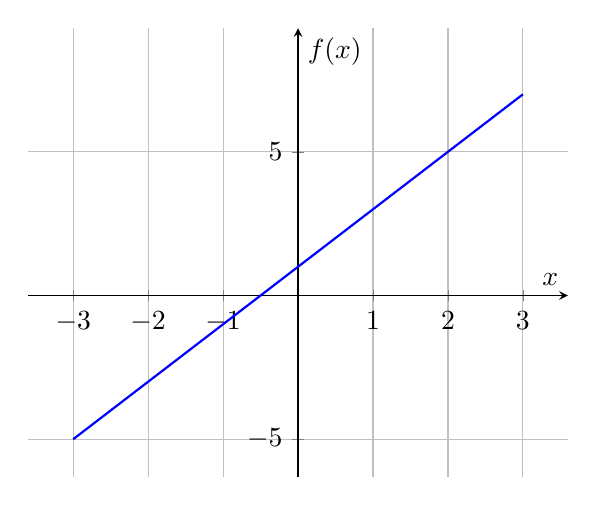
\begin{tikzpicture}
\begin{axis}[
    axis lines = middle,
    xlabel = $x$,
    ylabel = $f(x)$,
    domain=-3:3,
    samples=100,
    ymin=-5, ymax=8,
    xmin=-3, xmax=3,
    grid=both,
    enlargelimits=true
]
\addplot[blue, thick] {2*x + 1};
\end{axis}
\end{tikzpicture}
\]

This graph represents the function \( f(x) = 2x + 1 \), which is injective because each \( x \) value corresponds to a unique \( f(x) \) value.

To show why it is injective, assume \( f(a) = f(b) \):

\( 2a + 1 = 2b + 1 \)

Subtract 1 from both sides:

\( 2a = 2b \)

Divide by 2:

\( a = b \)

Thus, if \( f(a) = f(b) \), then \( a = b \). Hence, the function is injective.
} {}{NOTAGS} 
 
 
 
 \ex
{\code{FxGx24x12x28x004}}{20}
{
Draw a graph which is a function but not one-to-one.  
Why is it a non one-to-one function?
} {

 

A function that is not one-to-one has at least two different inputs that produce the same output. An example of such a function is \( f(x) = x^2 \), which is a parabola opening upwards. The graph of this function is not one-to-one because both positive and negative values of \( x \) yield the same \( f(x) \).

To illustrate this, consider:

\[
\begin{array}{ccc}
f(x) = x^2 & \text{for } x \in \mathbb{R} \\
f(1) = 1^2 = 1 & \\
f(-1) = (-1)^2 = 1 & \\
\Rightarrow f(1) = f(-1)
\end{array}
\]

The graph of \( f(x) = x^2 \) is:

\[
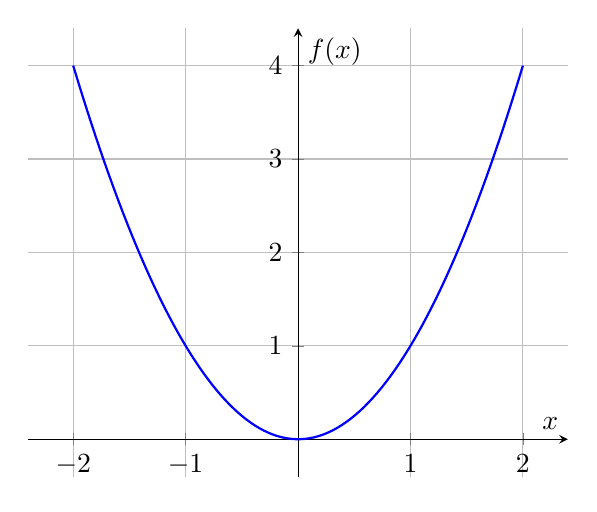
\begin{tikzpicture}
\begin{axis}[
    axis x line=middle, 
    axis y line=middle, 
    enlargelimits, 
    grid = major,
    xlabel = $x$,
    ylabel = {$f(x)$},
    domain=-2:2,
    samples=100
]
\addplot[thick,blue] {x^2};
\end{axis}
\end{tikzpicture}
\]

In this graph, it's clear that the function is not one-to-one since the horizontal line \( y = 1 \) intersects the graph at multiple points, specifically at \( (1,1) \) and \( (-1,1) \).

The function fails the horizontal line test, confirming it is not one-to-one.
} {}{NOTAGS} 
 
 
 
 \ex
{\code{FxGx24x12x28x005}}{20}
{
Draw a graph which is a function but not injective.  
Why is it a non injective function?
} {

 

A good response:

A non-injective graph example can be that of a parabola representing a quadratic function such as \( f(x) = x^2 \).

The graph of \( f(x) = x^2 \) is a U-shaped curve (parabola) that opens upwards.

This function is non-injective because there are distinct values of \( x \) that yield the same \( f(x) \) value. For example, \( f(a) = f(-a) \) for any \( a \in \mathbb{R} \) since \( f(x) = x^2 \).

In conclusion: 

A function is non-injective if there exist two different inputs, say \( x_1 \) and \( x_2 \), such that \( x_1 \neq x_2 \) but \( f(x_1) = f(x_2) \).

For the given function \( f(x) = x^2 \), it holds that \( f(1) = f(-1) = 1 \), demonstrating that it is not injective.
} {}{NOTAGS} 
 
 
 
 \ex
{\code{FxGx24x12x28x006}}{20}
{
Draw the graph of a function whose domain is all reals, and which is decreasing left of 4 and increasing right of 4.
Is it possible for such a function to be one-to-one? Explain.
}
{

 

A possible graph of a function satisfying these conditions is $f(x) = (x-4)^2$. This function is decreasing for $x < 4$ and increasing for $x > 4$. Below is a sketch of the graph:

\[
\begin{tikzpicture}[scale=0.8]
\draw[<->] (-1, 5) -- (-1, -1) -- (9, -1);
\draw[domain=-1:9, samples=100] plot (\x, {(\x-4)^2 -1});
\draw[dashed] (4, -1) -- (4, 15);
\node at (4, -0.2) [below] {4};
\node at (-0.8, 14.5) [left] {$y$};
\node at (8.8, -0.2) [right] {$x$};
\end{tikzpicture}
\]

Such a function cannot be one-to-one. A one-to-one function must pass the horizontal line test, meaning each horizontal line should intersect the graph at most once. Due to the symmetry and the turning point at $x = 4$, every horizontal line that crosses the vertex intersects the graph at two points, one on each side of the vertex, violating the horizontal line test.
} {}{NOTAGS}


\subsection{Finding Intercepts \topic{INT} }

\ex
{\code{FxINTx25x01x21x002}}{20}
{
Consider the graph of \(y = x^2 + x - 6\). Find all its intercepts (both \(x\)- and \(y\)-intercepts).
}
{

 

The \(y\)-intercept of the graph is found by setting \(x = 0\):

\[
y = 0^2 + 0 - 6 = -6
\]

So, the \(y\)-intercept is \((0, -6)\).

To find the \(x\)-intercepts, set \(y = 0\):

\[
x^2 + x - 6 = 0
\]

Factor the quadratic:

\[
(x+3)(x-2) = 0
\]

Setting each factor to zero gives:

\[
x+3 = 0 \quad \Rightarrow \quad x = -3
\]
\[
x-2 = 0 \quad \Rightarrow \quad x = 2
\]

So, the \(x\)-intercepts are \((-3, 0)\) and \((2, 0)\).
} {}{NOTAGS}


\subsection{Parabola Basics \topic{PB}} 


\ex
{\code{FxGPx25x02x18x001}}{5}
{
Consider the parabola \(f(x)=2x^2 +8x+3\).
Find its axis of symmetry.

}
{

 

The axis of symmetry for a parabola given by the function \(f(x) = ax^2 + bx + c\) is found using the formula:

\[ x = -\frac{b}{2a} \]

For the parabola \(f(x) = 2x^2 + 8x + 3\), we have \(a = 2\) and \(b = 8\).

Substitute these values into the formula for the axis of symmetry:

\[ x = -\frac{8}{2 \times 2} = -\frac{8}{4} = -2 \]

Thus, the axis of symmetry is:

\[ x = -2 \]
} {}{NOTAGS}

\ex
{\code{FxGPx25x02x18x002}}{5}
{
Consider the parabola \(f(x)=3x^2 - 6x + 30\).
Find its axis of symmetry.

}
{

 

The axis of symmetry for a parabola given by \(f(x) = ax^2 + bx + c\) is found using the formula:

\[ x = -\frac{b}{2a} \]

For the given parabola \(f(x) = 3x^2 - 6x + 30\), we have \(a = 3\) and \(b = -6\).

Substituting these values into the formula, we get:

\[ x = -\frac{-6}{2 \cdot 3} = \frac{6}{6} = 1 \]

Thus, the axis of symmetry is:

\[ x = 1 \]
} {}{NOTAGS}


\ex
{\code{FxGPx25x02x18x005}}{10}
{
Write the parabola \(h(x)= (x - 2)^2 + 1\) in
in general form.

}
{

 

\(h(x) = (x - 2)^2 + 1\)

Expanding the squared term:

\((x - 2)^2 = x^2 - 4x + 4\)

Substitute back into the equation:

\(h(x) = x^2 - 4x + 4 + 1\)

Simplify:

\(h(x) = x^2 - 4x + 5\)

So, the general form is:

\(h(x) = x^2 - 4x + 5\)
} {}{NOTAGS}

\ex
{\code{FxGPx25x02x18x006}}{10}
{
Write the parabola \(f(x)= (x + 4)^2 - 2\) in
in general form.

}
{

 

\(f(x) = (x + 4)^2 - 2\)

Expanding \( (x + 4)^2 \):

\((x + 4)^2 = x^2 + 8x + 16\)

Thus, 

\(f(x) = x^2 + 8x + 16 - 2\)

Simplifying, we get:

\(f(x) = x^2 + 8x + 14\)

The general form is:

\(f(x) = x^2 + 8x + 14\)
} {}{NOTAGS}


\ex
{\code{HWxFxGPx25x02x18x103}}{15}
{
Write the parabola \(g(x)=x^2 - 12x + 32\)
in vertex form.

}
{

 

\[
g(x) = x^2 - 12x + 32
\]

To write the parabola in vertex form, complete the square:

\[
g(x) = (x^2 - 12x) + 32
\]

Take half of \(-12\), square it, and add inside the parentheses:

\[
g(x) = (x^2 - 12x + 36 - 36) + 32
\]

\[
g(x) = ((x - 6)^2 - 36) + 32
\]

Simplify:

\[
g(x) = (x - 6)^2 - 4
\]

The vertex form is:

\[
g(x) = (x - 6)^2 - 4
\]
} {}{type: HW}

\ex
{\code{FxGPx25x02x18x004}}{15}
{
Write the parabola \(g(x)=x^2 - x\)
in vertex form.

}
{

 

\(g(x) = x^2 - x\)

To convert to vertex form, complete the square:

\(g(x) = x^2 - x\)

Factor out the coefficient of \(x^2\):

\(g(x) = (x^2 - x)\)

Complete the square inside the parentheses:

\(g(x) = (x^2 - x + \left(\frac{-1}{2}\right)^2 - \left(\frac{-1}{2}\right)^2)\)

\(g(x) = \left(x - \frac{1}{2}\right)^2 - \frac{1}{4}\)

Vertex form:

\(g(x) = \left(x - \frac{1}{2}\right)^2 - \frac{1}{4}\)
} {}{NOTAGS}


\ex
{\code{TESTxFxGPx25x02x18x001}}{15}
{
Write the parabola \(f(x)=x^2 + 2x - 3\)
in vertex form.

}
{

 

\(f(x) = (x+1)^2 - 4\)
} {}{NOTAGS}


\ex
{\code{TESTxFxGPx25x02x18x002}}{10}
{
Write the parabola \(f(x)= (x - 1)^2\) in
in general form.

}
{

 

\(f(x) = (x - 1)^2\)

\[ 
f(x) = x^2 - 2x + 1 
\]
} {}{NOTAGS}


\subsection{Graphing Parabolas \topic{GP}} 
 
 
\ex
{\code{HWxFxGPx25x02x18x102}}{15}
{
What is the domain and range of the quadratic function
 $f(x)=(x - 7)^2 + 3$.

}
{

 

\text{The domain of } $f(x)=(x - 7)^2 + 3 \text{ is } \mathbb{R}.$

\text{The range of } $f(x) \text{ is } [3, \infty).$
} {}{type: HW} 


\ex
{\code{FxGPx25x02x18x003}}{15}
{
What is the domain and range of the quadratic function
 \(f(x)=(x + 8)^2  - 9\).

}
{

 

The domain of \(f(x) = (x + 8)^2 - 9\) is all real numbers, since any real number can be used for \(x\).

The range of \(f(x)\) is determined by the values \(f(x)\) can take. Since \((x + 8)^2\) is the square of a real number, it is always non-negative, with a minimum value of 0. Thus, 

\[
(x + 8)^2 \geq 0
\]

Subtracting 9 from both sides gives:

\[
(x + 8)^2 - 9 \geq -9
\]

Therefore, the minimum value of \(f(x)\) is \(-9\). Hence, the range of \(f(x)\) is \([-9, \infty)\).

Thus, the domain and range are:

Domain: \((-\infty, \infty)\)

Range: \([-9, \infty)\)
} {}{NOTAGS} 

\ex
{\code{TESTxFxGPx25x02x18x007}}{20}
{
What is the domain and range of the quadratic function
 \(f(x)= 2x^2 - 6x\).

}
{

 

The domain of \(f(x) = 2x^2 - 6x\) is all real numbers, \(\mathbb{R}\).

To find the range, first rewrite the function in vertex form. Complete the square:

\[
f(x) = 2(x^2 - 3x)
\]

Complete the square inside the parentheses:

\[
x^2 - 3x = (x - \frac{3}{2})^2 - \left(\frac{3}{2}\right)^2
\]

\[
= (x - \frac{3}{2})^2 - \frac{9}{4}
\]

Now substitute back:

\[
f(x) = 2((x - \frac{3}{2})^2 - \frac{9}{4})
\]

\[
= 2(x - \frac{3}{2})^2 - \frac{18}{4}
\]

\[
= 2(x - \frac{3}{2})^2 - \frac{9}{2}
\]

The vertex form is \(f(x) = 2(x - \frac{3}{2})^2 - \frac{9}{2}\), indicating the vertex \(\left(\frac{3}{2}, -\frac{9}{2}\right)\) and the parabola opens upwards.

The minimum value of \(f(x)\) is \(-\frac{9}{2}\).

Thus, the range of \(f(x)\) is \([-{\frac{9}{2}}, \infty)\).

The solution is:

\text{Domain:} \ $\mathbb{R}$

\text{Range:} \ $[-\frac{9}{2}, \infty)$
} {}{NOTAGS} 


\ex
{\code{TESTxFxGPx25x02x18x006}}{20}
{
What is the domain and range of the quadratic function
 \(g(x)= 3x^2  - 6x - 9\).

}
{

 

The domain of the function \(g(x) = 3x^2 - 6x - 9\) is all real numbers, since a quadratic function is defined for every real \(x\).

The range can be determined from the vertex. The standard form of a quadratic function is \(a(x-h)^2 + k\), where \((h, k)\) is the vertex. Completing the square:

\[
g(x) = 3(x^2 - 2x) - 9
\]

\[
= 3((x-1)^2 - 1) - 9
\]

\[
= 3(x-1)^2 - 3 - 9
\]

\[
= 3(x-1)^2 - 12
\]

The vertex is \((1, -12)\), and since the parabola opens upwards (the coefficient of \((x-1)^2\) is positive), the minimum value of \(g(x)\) is \(-12\).

Therefore, the range of \(g(x)\) is \([-12, \infty)\).

Domain: \((-\infty, \infty)\)

Range: \([-12, \infty)\)
} {}{NOTAGS} 
 

\ex
{\code{FxGPx25x01x21x011}}{50}
{
Consider \(f(x)=2x^2 +8x+3\).

\begin{multicols}{2}
\begin{enumerate}
\item Does \(f\) open up or down?
\item Find its axis of symmetry.
\item Find the vertex.
\item What are the max/min values (if any)?
\item Sketch a rough graph (label the vertex).
\end{enumerate}
\end{multicols}
}
{

 

$f(x) = 2x^2 + 8x + 3$

\begin{enumerate}
    \item The function opens up because the coefficient of $x^2$ is positive.
    \item The axis of symmetry is given by $x = -\frac{b}{2a}$. Here, $a = 2$ and $b = 8$. So, the axis of symmetry is $x = -\frac{8}{2 \times 2} = -2$.
    \item The vertex is at $\left(-2, f(-2)\right)$. Calculate $f(-2)$:
    \[
    f(-2) = 2(-2)^2 + 8(-2) + 3 = 2(4) - 16 + 3 = 8 - 16 + 3 = -5
    \]
    Thus, the vertex is $(-2, -5)$.
    \item Since the parabola opens up, the vertex represents a minimum value. The minimum value is $-5$.
    \item Sketch: Draw a parabola opening upwards with vertex labeled at $(-2, -5)$ and axis of symmetry $x = -2$.
\end{enumerate}
} {}{NOTAGS}


\ex
{\code{FxGPx25x01x22x001}}{20}
{
Consider the parabola \(y - 9x^2 = x\). Do \emph{not} graph it, but do the following:

\begin{enumerate}
\item Write the equation in standard form.
\item Find the axis of symmetry.
\item Find its \(x\)- and \(y\)-intercepts.
\end{enumerate}
}{

 

\begin{enumerate}
\item The given equation is \(y - 9x^2 = x\). Rearrange it to standard form:

\[
y = 9x^2 + x
\]

Thus, the standard form is:

\[
y = 9x^2 + x
\]

\item The standard form of a parabola \(y = ax^2 + bx + c\) has an axis of symmetry given by \(x = -\frac{b}{2a}\). For the equation \(y = 9x^2 + x\), \(a = 9\) and \(b = 1\), so:

\[
x = -\frac{1}{2 \cdot 9} = -\frac{1}{18}
\]

Therefore, the axis of symmetry is:

\[
x = -\frac{1}{18}
\]

\item To find the \(x\)-intercepts, set \(y = 0\):

\[
0 = 9x^2 + x
\]
\[
x(9x + 1) = 0
\]

The solutions are:

\[
x = 0 \quad \text{or} \quad x = -\frac{1}{9}
\]

Thus, the \(x\)-intercepts are:

\[
(0, 0) \quad \text{and} \quad \left(-\frac{1}{9}, 0\right)
\]

To find the \(y\)-intercept, set \(x = 0\):

\[
y = 9(0)^2 + 0 = 0
\]

Thus, the \(y\)-intercept is:

\[
(0, 0)
\]
\end{enumerate}
}{}{NOTAGS}

\ex
{\code{FxGPx25x01x22x002}}{30}
{
Consider the parabola \(y + 3x = -x^2\). 

\begin{enumerate}
\item Find its intercepts.
\item Find the vertex.
\item Find a pair of points symmetric about the axis.
\item Graph the parabola.
\end{enumerate}
}{

 

Solve for \(y\) in terms of \(x\):

\[
y = -x^2 - 3x
\]

1. **Intercepts:**

   - **y-intercept:**

     Set \(x = 0\):

     \[
     y = -(0)^2 - 3(0) = 0
     \]

     So, the y-intercept is \((0, 0)\).

   - **x-intercepts:**

     Set \(y = 0\):

     \[
     0 = -x^2 - 3x
     \]

     Factor out the common term:

     \[
     0 = -x(x + 3)
     \]

     Solving, we find \(x = 0\) or \(x = -3\).

     So, the x-intercepts are \((0, 0)\) and \((-3, 0)\).

2. **Vertex:**

   The vertex form of a parabola is \(y = a(x - h)^2 + k\).

   The equation is \(y = -x^2 - 3x\), so:

   Comparing with the standard form \(y = ax^2 + bx + c\):
   
   \(a = -1\), \(b = -3\)

   The vertex \(h = -\frac{b}{2a} = -\frac{-3}{2(-1)} = \frac{3}{2}\).

   Substitute \(x = \frac{3}{2}\) into the equation to find \(k\):

   \[
   y = -\left(\frac{3}{2}\right)^2 - 3\left(\frac{3}{2}\right)
   \]

   \[
   y = -\frac{9}{4} - \frac{9}{2} = -\frac{9}{4} - \frac{18}{4} = -\frac{27}{4}
   \]

   The vertex is \(\left(\frac{3}{2}, -\frac{27}{4}\right)\).

3. **Symmetric Points:**

   Choose a point \(x = 1\). Then \(x = 3 - 1 = 2\) will be symmetric around \(x = \frac{3}{2}\).

   For \(x = 1\):

   \[
   y = -(1)^2 - 3(1) = -1 - 3 = -4
   \]

   For \(x = 2\):

   \[
   y = -(2)^2 - 3(2) = -4 - 6 = -10
   \]

   Points symmetric about the axis: \((1, -4)\) and \((2, -10)\).

4. **Graph:**

   To graph the parabola, use the vertex, intercepts, and symmetric points identified:

   - Vertex: \(\left(\frac{3}{2}, -\frac{27}{4}\right)\)
   - y-intercept: \((0, 0)\)
   - x-intercepts: \((0, 0)\) and \((-3, 0)\)
   - Symmetric points: \((1, -4)\) and \((2, -10)\)

   Plot these points and draw a smooth curve through them to represent the parabola.


}{}{NOTAGS}





\ex
{\code{FxGPx25x02x03x001}}{50}
{
For the quadratic function $f(x)=(x-4)^2-1$
\begin{enumerate}
\item Find its vertex 

\item Find its $x$- and $y$-intercepts.

\item Give the equation of the axes of
symmetry.
 
\item Draw the graph.

\item Determine its domain and range.
\end{enumerate}

}{

 

\begin{enumerate}
\item The vertex of the function $f(x) = (x-4)^2 - 1$ is at $(4, -1)$.

\item To find the $x$-intercepts, set $f(x) = 0$:

\[
(x-4)^2 - 1 = 0 
\]

\[
(x-4)^2 = 1
\]

\[
x-4 = \pm 1
\]

\[
x = 5 \quad \text{or} \quad x = 3
\]

The $x$-intercepts are $(5, 0)$ and $(3, 0)$.

For the $y$-intercept, set $x = 0$:

\[
f(0) = (0-4)^2 - 1 = 16 - 1 = 15
\]

The $y$-intercept is $(0, 15)$.

\item The equation of the axis of symmetry is $x = 4$.

\item The graph of the function is a parabola opening upwards with vertex $(4, -1)$ and axis of symmetry $x = 4$.

\item The domain of the function is $(-\infty, \infty)$.

The range of the function is $[-1, \infty)$.
\end{enumerate}
}{}{NOTAGS}


\ex
{\code{FxGPx25x02x03x002}}{50}
{
For the quadratic function $g(x) = 4-(x-1)^2$
\begin{enumerate}
\item Find its vertex 

\item Find its $x$- and $y$-intercepts.

\item Give the equation of the axes of
symmetry.
 
\item Draw the graph.

\item Determine its domain and range.
\end{enumerate}

}{

 

The quadratic function is \( g(x) = 4 - (x-1)^2 \).

\begin{enumerate}
    \item \textbf{Vertex:} \\
    The function \( g(x) = 4 - (x-1)^2 \) is in the form \( g(x) = a(x-h)^2 + k \) with \( a = -1 \), \( h = 1 \), and \( k = 4 \). \\
    Therefore, the vertex is \( (1, 4) \).

    \item \textbf{\(x\)- and \(y\)-intercepts:} \\
    \textit{\(y\)-intercept:} Set \( x = 0 \). \\
    \( g(0) = 4 - (0-1)^2 = 4 - 1 = 3 \). \\
    So, the \(y\)-intercept is \( (0, 3) \). \\
    \textit{\(x\)-intercepts:} Set \( g(x) = 0 \). \\
    \( 4 - (x-1)^2 = 0 \) implies \( (x-1)^2 = 4 \). \\
    Solving gives \( x-1 = \pm 2 \), so \( x = 3 \) or \( x = -1 \). \\
    Thus, the \(x\)-intercepts are \( (3, 0) \) and \( (-1, 0) \).

    \item \textbf{Equation of the axis of symmetry:} \\
    The axis of symmetry is the vertical line through the vertex. \\
    Thus, the equation is \( x = 1 \).

    \item \textbf{Graph:} \\
    The graph is a parabola opening downwards with vertex at \( (1, 4) \). It intercepts the \(y\)-axis at \( (0, 3) \) and the \(x\)-axis at \( (3, 0) \) and \( (-1, 0) \).

    \item \textbf{Domain and Range:} \\
    \textit{Domain:} The domain of \( g(x) \) is all real numbers, \(\mathbb{R}\). \\
    \textit{Range:} The range of \( g(x) \) is \( g(x) \leq 4 \), so the range is \( (-\infty, 4] \).
\end{enumerate}
}{}{NOTAGS}


\ex
{\code{FxGPx25x02x03x003}}{50}
{
For the quadratic function $h(x)=3x^2-2x-4$
\begin{enumerate}
\item Find its vertex 

\item Find its $x$- and $y$-intercepts.

\item Give the equation of the axes of
symmetry.
 
\item Draw the graph.

\item Determine its domain and range.
\end{enumerate}

}{

 

For the quadratic function \( h(x) = 3x^2 - 2x - 4 \):

\begin{enumerate}
    \item \textbf{Vertex:} The vertex \((h, k)\) of a quadratic function \( ax^2 + bx + c \) can be found using \( h = -\frac{b}{2a} \).
    \[
    h = -\frac{-2}{2 \times 3} = \frac{1}{3}
    \]
    \[
    k = h\left(\frac{1}{3}\right) = 3\left(\frac{1}{3}\right)^2 - 2\left(\frac{1}{3}\right) - 4
    \]
    \[
    k = 3 \times \frac{1}{9} - \frac{2}{3} - 4 = \frac{1}{3} - \frac{2}{3} - 4 = -4.333
    \]
    Vertex: \(\left( \frac{1}{3}, -\frac{13}{3} \right)\)

    \item \textbf{Intercepts:}
    \begin{itemize}
        \item \(x\)-intercepts: Solve \(3x^2 - 2x - 4 = 0\) using the quadratic formula \(x = \frac{-b \pm \sqrt{b^2 - 4ac}}{2a}\).
        \[
        x = \frac{2 \pm \sqrt{(-2)^2 - 4 \times 3 \times (-4)}}{6}
        \]
        \[
        x = \frac{2 \pm \sqrt{4 + 48}}{6} = \frac{2 \pm \sqrt{52}}{6} = \frac{2 \pm 2\sqrt{13}}{6}
        \]
        \[
        x = \frac{1 \pm \sqrt{13}}{3}
        \]

        \item \(y\)-intercept: Evaluate \(h(x)\) at \(x = 0\).
        \[
        h(0) = -4
        \]
        \(y\)-intercept: \((0, -4)\)
    \end{itemize}

    \item \textbf{Axis of Symmetry:} Given by \(x = -\frac{b}{2a} = \frac{1}{3}\).

    \item \textbf{Graph:} Sketch a parabola opening upwards with the vertex at \(\left( \frac{1}{3}, -\frac{13}{3} \right)\),
    intercepts at \(\left(\frac{1 \pm \sqrt{13}}{3}, 0\right)\) and \((0, -4)\), and axis of symmetry \(x = \frac{1}{3}\).

    \item \textbf{Domain and Range:}
    \begin{itemize}
        \item Domain: \(\mathbb{R}\)
        \item Range: \([-\frac{13}{3}, \infty)\)
    \end{itemize}
\end{enumerate}
}{}{NOTAGS}







\ex
{\code{FxGPx25x01x22x004}}{25}
{
The number of people (\(P\)) infected \(t\) days after a flu outbreak is modeled by
\(P(t) = -t^2 + 100t + 20\). 

\begin{enumerate}
\item How many days after outbreak is the maximum number sick?
\item What is that maximum number of people infected at once?
\end{enumerate}
}{

 

\begin{enumerate}
\item To find the number of days after the outbreak when the maximum number of people are infected, we need to find the vertex of the parabola given by \(P(t) = -t^2 + 100t + 20\). The vertex \(t\) for a quadratic \(at^2 + bt + c\) is given by \(t = -\frac{b}{2a}\).

\[
t = -\frac{100}{2(-1)} = \frac{100}{2} = 50
\]

So, the maximum number of people are infected 50 days after the outbreak.

\item To find the maximum number of people infected, we substitute \(t = 50\) into \(P(t)\):

\[
P(50) = -(50)^2 + 100(50) + 20
\]

\[
= -2500 + 5000 + 20
\]

\[
= 2520
\]

The maximum number of people infected at once is 2520.
\end{enumerate}
}{}{NOTAGS}

\ex
{\code{FxGPx25x01x22x005}}{25}
{
A patient's body temperature \(T\) (in Fahrenheit) \(x\) hours after acetaminophen is
\(T(x) = 0.4x^2 - 2.6x + 103\). 

\begin{enumerate}
\item When will the temperature be minimum?
\item What is that minimum temperature?
\end{enumerate}
}{

 

\junk{
The given function for the patient's body temperature is

\[ T(x) = 0.4x^2 - 2.6x + 103 \]

To find the time \(x\) when the temperature is minimum, we need to find the vertex of the parabola. In a quadratic function \(ax^2 + bx + c\), the vertex occurs at \(x = -\frac{b}{2a}\).

Here, \(a = 0.4\) and \(b = -2.6\).

The time \(x\) when the temperature is minimum is:

\[ x = -\frac{-2.6}{2 \times 0.4} = \frac{2.6}{0.8} = 3.25 \]

Therefore, the temperature will be minimum at \(x = 3.25\) hours.

Now, to find the minimum temperature, substitute \(x = 3.25\) back into the function:

\begin{align*}
T(3.25) & = 0.4(3.25)^2 - 2.6(3.25) + 103 \\
        & = 0.4(10.5625) - 8.45 + 103 \\
        & = 4.225 - 8.45 + 103 \\
        & = 98.775
\end{align*}


The minimum temperature is \(98.775\) degrees Fahrenheit.
}
}{}{NOTAGS}



\ex
{\code{HWxFxGPx25x01x22x003}}{30}
{
Consider $y = x^2 + 5x + 6$. 

\begin{enumerate}
\item Find all intercepts.
\item Find the point on the graph with maximum \(y\) (or explain if none).
\item Find the point on the graph with minimum \(y\) (or explain if none).
\item Graph the equation.
\end{enumerate}
}{

 

\begin{enumerate}
    \item To find the intercepts:
    \begin{itemize}
        \item \textbf{y-intercept:} Set \(x = 0\).
        \[
        y = 0^2 + 5(0) + 6 = 6
        \]
        The y-intercept is \((0, 6)\).
        \item \textbf{x-intercepts:} Set \(y = 0\).
        \[
        0 = x^2 + 5x + 6
        \]
        Factor the quadratic:
        \[
        0 = (x+2)(x+3)
        \]
        Thus, \(x = -2\) and \(x = -3\). The x-intercepts are \((-2, 0)\) and \((-3, 0)\).
    \end{itemize}
    
    \item There is no maximum point since the parabola opens upwards (\(a = 1 > 0\)).

    \item The minimum point occurs at the vertex. For a quadratic \(ax^2 + bx + c\), the vertex \(x\)-coordinate is:
    \[
    x = -\frac{b}{2a} = -\frac{5}{2 \times 1} = -\frac{5}{2}
    \]
    Substitute back to find \(y\):
    \[
    y = \left(-\frac{5}{2}\right)^2 + 5\left(-\frac{5}{2}\right) + 6 = \frac{25}{4} - \frac{25}{2} + 6 = -\frac{1}{4}
    \]
    The minimum point is \(\left(-\frac{5}{2}, -\frac{1}{4}\right)\).
    
    \item Graph the equation: 
    
    The graph is a parabola opening upwards with vertex at \(\left(-\frac{5}{2}, -\frac{1}{4}\right)\), y-intercept at \((0, 6)\), and x-intercepts at \((-2, 0)\) and \((-3, 0)\).
\end{enumerate}
}{}{type: HW}


\ex
{\code{HWxFxGPx25x02x03x004}}{50}
{
For the quadratic function $f(x) = 2x-x^2-2$
\begin{enumerate}
\item Find its vertex 

\item Find its $x$- and $y$-intercepts.

\item Give the equation of the axes of
symmetry.
 
\item Draw the graph.

\item Determine its domain and range.
\end{enumerate}

}{

 

The given quadratic function is \( f(x) = 2x - x^2 - 2 \).

\begin{enumerate}
    \item \textbf{Find its vertex:}

    The standard form of a quadratic function is \( f(x) = ax^2 + bx + c \). Here, \( a = -1 \), \( b = 2 \), \( c = -2 \).

    The vertex \((h, k)\) can be found using the formulas:
    \[
    h = -\frac{b}{2a} = -\frac{2}{2(-1)} = 1
    \]
    \[
    k = f(h) = f(1) = 2(1) - (1)^2 - 2 = 2 - 1 - 2 = -1
    \]
    Thus, the vertex is \((1, -1)\).

    \item \textbf{Find its $x$- and $y$-intercepts:}

    - $y$-intercept: Set \( x = 0 \).
      \[
      f(0) = 2(0) - (0)^2 - 2 = -2
      \]
      So, the $y$-intercept is \( (0, -2) \).

    - $x$-intercepts: Set \( f(x) = 0 \).
      \[
      2x - x^2 - 2 = 0 \quad \Rightarrow \quad -x^2 + 2x - 2 = 0
      \]
      \[
      x^2 - 2x + 2 = 0
      \]
      The discriminant \(\Delta = b^2 - 4ac = (-2)^2 - 4(1)(2) = 4 - 8 = -4\).

      Since \(\Delta < 0\), there are no real $x$-intercepts.

    \item \textbf{Give the equation of the axis of symmetry:}

    The axis of symmetry is given by \( x = h \).
    \[
    x = 1
    \]

    \item \textbf{Draw the graph:}

    (Graph not shown, but the key points and vertex form a parabola opening downwards. The vertex is \((1, -1)\), with \( y \)-intercept \((0, -2)\).)

    \item \textbf{Determine its domain and range:}

    - Domain: The domain of a quadratic function is \( \mathbb{R} \).

    - Range: Since the parabola opens downward, the range is \( y \leq -1 \).

    Thus, the range is \( (-\infty, -1] \).

\end{enumerate}
}{}{type: HW}




\ex
{\code{TESTxFxGPx25x02x18x004}}{15}
{
What is the domain and range of the quadratic function
 \(f(x)=(x - 3)^2  + 1\).

}
{

 

The domain of the function \(f(x) = (x - 3)^2 + 1\) is all real numbers, denoted as:

\(\text{Domain: } (-\infty, \infty)\)

The range of the function is determined by the minimum value of \((x - 3)^2 + 1\). Since \((x - 3)^2 \geq 0\), the minimum value occurs when \((x - 3)^2 = 0\), which gives \(f(x) = 1\). Therefore, the range is:

\(\text{Range: } [1, \infty)\)
} {}{NOTAGS} 

\ex
{\code{TESTxFxGPx25x02x18x005}}{25}
{
What is the domain and range of the quadratic function
 \(g(x)= x^2  + 6x + 4\).

}
{

SOLUTION:

Domain: All reals.

\vspace{2mm}

Range: First find the $x$ coordinate of the vertex, from the axis of symmetry (from $x = \dfrac{-b}{2a}$),
that is: $x = \dfrac{- 6}{2(1)}$, so $x = -3$.

To find the $y$ coordinate of the vertex:
$g(-3) = 9 - 18 + 4 = -5$, so the vertex is $(-3, -5)$.

Since this parabola opens up, the range is:
All reals $y \ge -5$.

} {}{NOTAGS} 




\ex 
{\code{TESTxxxFxGPx25x03x27x001}}{30}
{
The amount of money in dollars (\(M\)) in the school's bank account  \(t\) days after it opens is modeled by
\(M(t) = 2t^2 - 20t + 85\). 

\begin{enumerate}
\item How many days after the school opens is the bank account's minimum reached?
\item What is that minimum amount of money in the bank account?
\end{enumerate}
}{

SOLUTION:

This parabola opens up, so has a minimum at its vertex.

\vspace{2mm}

For (a): Find the axis of symmetry ($t = \dfrac{-b}{2a}$), so
$t = \dfrac{-(-20)}{2(2)}$, so $t = 5$.  So the minimum occurs when $t = 5$, so after 5 days.

\vspace{2mm}

For (b): Find the $y$ coordinate of the vertex, by
$M(5) = 50 - 100 + 85 = 35$, so the minimum amount of money is $\$35$.

}{}{NOTAGS}



\subsection{Detailed Function Graphing \topic{GG}} 
 
 

 
 
 \ex
{\code{FxGGx24x12x28x001}}{70}
{
Graph the function, find its asymptotes, and find its domain and range:
$$g(x) = \dfrac{1}{(x -3)^2}$$

Also, describe its end behavior, and use arrow notation to describe the behavior at the undefined value.

} 
{
\solfig{FxGGx24x12x28x001}



} 
{
\begin{figure}[H] 
    \centering
    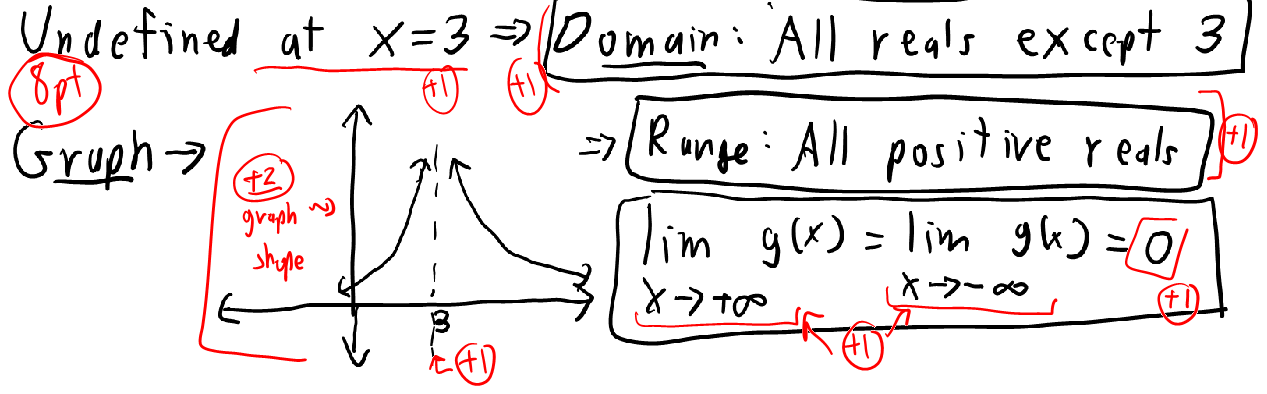
\includegraphics[scale=.7]{FigsRubrics/RUBRICxxxFxGGx24x12x28x001.pdf} 
\end{figure}
}{NOTAGS} 
 
 
 
 \ex
{\code{FxGGx24x12x28x002}}{70}
{
Graph the function, find its asymptotes, and find its domain and range:
$$g(x) = 2 + \dfrac{1}{(x -3)^5}$$

Also, describe its end behavior, and use arrow notation to describe the behavior at the undefined value.

} {

 

Graph:

The graph of \( g(x) = 2 + \dfrac{1}{(x - 3)^5} \) is a transformation of the basic reciprocal function \( \dfrac{1}{x^5} \). It is shifted 3 units to the right and 2 units up.

Asymptotes:

The function has a vertical asymptote at \( x = 3 \).

Domain and Range:

The domain of \( g(x) \) is all real numbers except \( x = 3 \). 
Thus, the domain is \( (-\infty, 3) \cup (3, \infty) \).

The range is all real numbers, \( \mathbb{R} \).

End Behavior:

As \( x \to \infty \) or \( x \to -\infty \), \( g(x) \to 2 \).

Arrow Notation:

- As \( x \to 3^- \), \( g(x) \to -\infty \).
- As \( x \to 3^+ \), \( g(x) \to \infty \).
} {}{NOTAGS} 
 
 
 
 \ex
{\code{FxGGx25x01x20x014}}{50}
{
Sketch the graph of the function \(g(x) = 1 - x^2\), 
and indicate the \(x\)- and \(y\)-intercepts.
} {

 

The function \(g(x) = 1 - x^2\) is a parabola that opens downward.

The \(y\)-intercept is:

When \(x = 0\),

\[
g(0) = 1 - 0^2 = 1
\]

So the \(y\)-intercept is \((0, 1)\).

The \(x\)-intercepts are:

Set \(g(x) = 0\),

\[
1 - x^2 = 0
\]

\[
x^2 = 1
\]

\[
x = \pm 1
\]

So the \(x\)-intercepts are \((-1, 0)\) and \((1, 0)\).

The vertex of the parabola is at \((0, 1)\).

The rough sketch of the graph is a downward-facing parabola, intersecting the \(y\)-axis at \((0, 1)\) and the \(x\)-axis at \((-1, 0)\) and \((1, 0)\).
} {}{NOTAGS} 
 
 
 
 \ex
{\code{FxGGx25x01x20x021}}{40}
{
 Sketch the two functions functions on the same coordinate plane.

\begin{multicols}{2}
\begin{enumerate}
\item $f(x) = x^2 + 1$
\item $g(x) = -2x^2 - 1$
\end{enumerate}
\end{multicols}
} {

 

\[
\begin{array}{c}
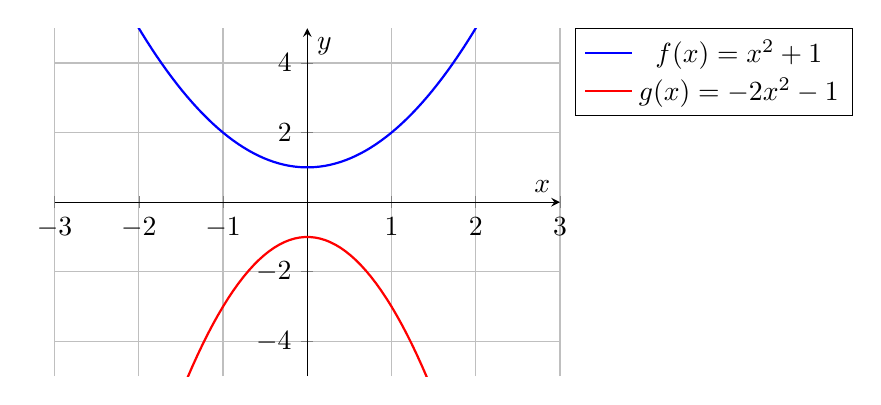
\begin{tikzpicture}
\begin{axis}[
    xlabel={$x$},
    ylabel={$y$},
    axis lines = center,
    grid = both,
    legend pos=outer north east,
    xmin=-3, xmax=3,
    ymin=-5, ymax=5,
    width=8cm, height=6cm,
    domain=-3:3
]
\addplot[blue, thick, samples=100] {x^2 + 1};
\addlegendentry{$f(x) = x^2 + 1$}

\addplot[red, thick, samples=100] {-2*x^2 - 1};
\addlegendentry{$g(x) = -2x^2 - 1$}
\end{axis}
\end{tikzpicture}
\end{array}
\]
} {}{NOTAGS} 
 
 
 
 \ex
{\code{FxGGx25x01x20x022}}{30}
{
Graph the following function:
$h(x) = x^2 - x - 56$

} {

 

To graph the function \( h(x) = x^2 - x - 56 \), we first find the vertex and axis of symmetry.

The vertex form of a quadratic function is \( h(x) = a(x-h)^2 + k \).

Given \( h(x) = x^2 - x - 56 \), we have:

- \( a = 1 \)
- \( b = -1 \)
- \( c = -56 \)

The axis of symmetry is given by \( x = -\frac{b}{2a} \).

\[
x = -\frac{-1}{2 \times 1} = \frac{1}{2}
\]

To find the vertex, substitute \( x = \frac{1}{2} \) into \( h(x) \):

\[
h\left(\frac{1}{2}\right) = \left(\frac{1}{2}\right)^2 - \frac{1}{2} - 56 = \frac{1}{4} - \frac{1}{2} - 56 = -\frac{1}{4} - 56 = -\frac{225}{4}
\]

Thus, the vertex is:

\[
\left( \frac{1}{2}, -\frac{225}{4} \right)
\]

The y-intercept is found by evaluating \( h(0) \):

\[
h(0) = 0^2 - 0 - 56 = -56
\]

The x-intercepts can be found by solving \( h(x) = 0 \):

\[
x^2 - x - 56 = 0
\]

Using the quadratic formula \( x = \frac{-b \pm \sqrt{b^2 - 4ac}}{2a} \):

\[
x = \frac{-(-1) \pm \sqrt{(-1)^2 - 4 \cdot 1 \cdot (-56)}}{2 \cdot 1}
\]

\[
x = \frac{1 \pm \sqrt{1 + 224}}{2} = \frac{1 \pm \sqrt{225}}{2}
\]

\[
x = \frac{1 \pm 15}{2}
\]

The solutions are \( x = 8 \) and \( x = -7 \).

Thus, the x-intercepts are \( x = 8 \) and \( x = -7 \).

These values and characteristics help us to graph the function:

- Vertex: \( \left( \frac{1}{2}, -\frac{225}{4} \right) \)
- Axis of Symmetry: \( x = \frac{1}{2} \)
- y-intercept: \( (0, -56) \)
- x-intercepts: \( (-7, 0) \) and \( (8, 0) \)
} {}{NOTAGS} 
 
 
\ex
{\code{FxGGx25x01x22x015}}{40}
{
Sketch $f(x) = 3^x$ and $g(x)=\log_{3}(x)$ on the same axes. Label any intercepts and coordinates.
}{

 

\junk{
\[
\begin{tikzpicture}
    \begin{axis}[
        axis lines = middle,
        xlabel = $x$, ylabel = $y$,
        xmin = 0, xmax = 4,
        ymin = -2, ymax = 4,
        domain = -2:4,
        samples = 100,
        xtick = {0, 1, 2, 3, 4},
        ytick = {-1, 0, 1, 2, 3, 4},
        legend pos = north west
    ]
    \addplot [blue, thick] {$3^x$};
    \addplot [red, thick, dashed] {$\log_{3}(x)$};
    
    \node at (axis cs:0.5,0.7) [anchor=west] {$y = \log_{3}(x)$};
    \node at (axis cs:1, 9) [anchor=west] {$y = 3^x$};
    
    \addplot[black, mark=*] coordinates {(0,1)} node[anchor=east] {$(0, 1)$};
    \addplot[black, mark=*] coordinates {(1,0)} node[anchor=north] {$(1, 0)$};
    
    \end{axis}
\end{tikzpicture}
\]
}
}{}{NOTAGS}
 
 
 
 \ex
{\code{FxGGx25x01x20x015}}{50}
{
 Sketch \(f(x) = 10^x\) and \(g(x) = \log_{10}(x)\) on the same axes (you may scale the \(y\)-axis).

What are the asymptotes of each graph?

Find any two points that are symmetric across the line \(y = x\).
} {

 

To sketch the graphs of \(f(x) = 10^x\) and \(g(x) = \log_{10}(x)\) on the same axes:

- The graph of \(f(x) = 10^x\) is an exponential curve that passes through the point \((0, 1)\) and increases rapidly. It has a horizontal asymptote at \(y = 0\).

- The graph of \(g(x) = \log_{10}(x)\) is a logarithmic curve that passes through the point \((1, 0)\) and increases slowly. It has a vertical asymptote at \(x = 0\).

To find two points that are symmetric across the line \(y = x\):

1. Choose a point on \(f(x)\), for instance, when \(x = 2\):

   \[
   f(2) = 10^2 = 100
   \]

   So the point is \((2, 100)\).

2. The symmetric point on \(g(x)\) would swap the coordinates:

   \[
   g(100) = \log_{10}(100) = 2
   \]

   So the symmetric point is \((100, 2)\).

Thus, the points \((2, 100)\) on \(f(x)\) and \((100, 2)\) on \(g(x)\) are symmetric across \(y = x\).

The asymptotes are:
- \(y = 0\) for \(f(x) = 10^x\).
- \(x = 0\) for \(g(x) = \log_{10}(x)\).
} {}{NOTAGS} 
 
 
 
 \ex
{\code{FxGGx25x01x20x016}}{50}
{
Sketch \(f(x) = 10^x\) and \(g(x) = 10^{-x}\) on the same axes.

What are the asymptotes of each graph?

Find any two points that are symmetric across the \(y\)-axis.
}
{

 

To solve this exercise, we will provide a visual sketch description and algebraic information.

**Graph Sketch:**

Draw the graph of \(f(x) = 10^x\):
- It's an exponential curve that passes through the point \((0,1)\).
- As \(x \to -\infty\), \(f(x) \to 0\).
- As \(x \to \infty\), \(f(x) \to \infty\).

Draw the graph of \(g(x) = 10^{-x}\):
- It's an exponential decay curve that also passes through the point \((0,1)\).
- As \(x \to -\infty\), \(g(x) \to \infty\).
- As \(x \to \infty\), \(g(x) \to 0\).

**Asymptotes:**

Both graphs have a horizontal asymptote:
- \(y = 0\).

**Symmetric Points:**

Select points on each graph where one is \((a, b)\) and the symmetric point is \((-a, b)\).

For \(f(x) = 10^x\):
- The point \((1, 10)\).

For \(g(x) = 10^{-x}\):
- The point \((-1, 10)\).

Thus, the points \((1, 10)\) and \((-1, 10)\) are symmetric across the \(y\)-axis.
} {}{NOTAGS}


 \ex
{\code{FxGGx25x02x03x001}}{70}
{
For the function $f(x)= 2 (x-2)^2 (x+1)$ , do the following:

\begin{multicols}{2}
\begin{enumerate}
\item Determine the end behaviour of the graph.

\item Find the $y$-intercept.

\item Find the $x$-intercepts with their 
multiplicity. Determine the local behaviour  (cross or touch?) at the $x$-intercepts.

\item Make a sketch of the graph.

\end{enumerate}
\end{multicols}
}
{

 

1. The function $f(x) = 2(x-2)^2(x+1)$ is a cubic function (degree 3). As $x \to \infty$, $f(x) \to \infty$, and as $x \to -\infty$, $f(x) \to -\infty$.

2. The $y$-intercept occurs when $x = 0$: $f(0) = 2(0-2)^2(0+1) = 2 \times 4 \times 1 = 8$. Thus, the $y$-intercept is $(0, 8)$.

3. To find the $x$-intercepts, set $f(x) = 0$: 
   \[
   2(x-2)^2(x+1) = 0 
   \]
   \[
   (x-2)^2 = 0 \quad \text{or} \quad (x+1) = 0 
   \]
   The solutions are $x = 2$ (with multiplicity 2) and $x = -1$ (with multiplicity 1).
   
   - At $x = 2$, the curve touches the $x$-axis and turns around (since the multiplicity is even).
   - At $x = -1$, the curve crosses the $x$-axis (since the multiplicity is odd).

4. Sketch:
   - Plot the $y$-intercept at $(0, 8)$.
   - Plot the $x$-intercepts at $x = 2$ and $x = -1$.
   - Sketch the end behavior: going to $-\infty$ as $x \to -\infty$ and to $\infty$ as $x \to \infty$.
   - The graph touches at $x = 2$ and crosses at $x = -1$.
} {}{NOTAGS}


 \ex
{\code{FxGGx25x02x03x002}}{70}
{
For the function $f(x)=-2 x^2(x-2) (x+2)^2$ , do the following:

\begin{multicols}{2}
\begin{enumerate}
\item Determine the end behaviour of the graph.

\item Find the $y$-intercept.

\item Find the $x$-intercepts with their 
multiplicity. Determine the local behaviour (cross or touch?) at the $x$-intercepts.

\item Make a sketch of the graph.

\end{enumerate}
\end{multicols}
}
{

 

1. **End Behaviour**:

The end behaviour of the polynomial function is determined by the highest degree term. Here, the function is:

\[ f(x) = -2x^2(x-2)(x+2)^2 \]

When expanded, the highest degree term will be:

\[ -2x^5 \]

Since the leading term is \(-2x^5\), as \(x \to \infty\), \(f(x) \to -\infty\) and as \(x \to -\infty\), \(f(x) \to \infty\).

2. **$y$-Intercept**:

To find the \(y\)-intercept, set \(x = 0\):

\[ f(0) = -2(0)^2(0-2)(0+2)^2 = -2 \times 0 \times (-2) \times 4 = 0 \]

So, the \(y\)-intercept is \((0, 0)\).

3. **$x$-Intercepts and Local Behaviour**:

Factor the function:

\[ f(x) = -2x^2(x-2)(x+2)^2 \]

- \(x = 0\) with multiplicity \(2\) (touches the x-axis and turns around).
- \(x = 2\) with multiplicity \(1\) (crosses the x-axis).
- \(x = -2\) with multiplicity \(2\) (touches the x-axis and turns around).

4. **Sketch of the Graph**:

\junk{
The graph should:

- Cross the x-axis at \(x = 2\).
- Touch and turn around at \(x = 0\) and \(x = -2\).
- Have the end behaviour \(x \to \infty, f(x) \to -\infty\) and \(x \to -\infty, f(x) \to \infty\).

\[
\begin{tikzpicture}[scale=0.5]

\draw[very thin,color=gray] (-5.1,-5.1) grid (5.1,5.1);
    
\draw[->] (-5.5,0) -- (5.5,0) node[right] {$x$};
\draw[->] (0,-5.5) -- (0,5.5) node[above] {$f(x)$};

\draw[domain=-3.2:3.2,smooth,variable=\x,blue] plot ({\x},{-2*\x*\x*(\x-2)*(\x+2)*(\x+2)}); 

\draw[fill] (0,0) circle [radius=0.1] node[anchor=north east] {(0,0)};
\draw[fill] (2,0) circle [radius=0.1] node[anchor=north west] {(2,0)};
\draw[fill] (-2,0) circle [radius=0.1] node[anchor=south east] {(-2,0)};

\end{tikzpicture}
\]
}
} {}{NOTAGS}

 \ex
{\code{FxGGx25x02x03x003}}{70}
{
For the function $f(x)=3 x (x+1)^2(x-1)^3$ , do the following:

\begin{multicols}{2}
\begin{enumerate}
\item Determine the end behaviour of the graph.

\item Find the $y$-intercept.

\item Find the $x$-intercepts with their 
multiplicity. Determine the local behaviour  (cross or touch?) at the $x$-intercepts.

\item Make a sketch of the graph.

\end{enumerate}
\end{multicols}
}
{

 

For the function \(f(x) = 3x(x+1)^2(x-1)^3\), do the following:

1. **End behaviour of the graph:**

   The leading term of \(f(x)\) is obtained from expanding the expression, primarily determined by the highest power of \(x\). The degree of \(f(x)\) is \(1 + 2 + 3 = 6\). Therefore, the leading term is \(3x^6\). Since the leading coefficient is positive and the degree is even, the end behaviour is:
   \[
   \text{As } x \to \pm \infty, \, f(x) \to \infty
   \]

2. **Find the \(y\)-intercept:**

   The \(y\)-intercept occurs when \(x = 0\):
   \[
   f(0) = 3 \cdot 0 \cdot (0+1)^2 \cdot (0-1)^3 = 0
   \]
   Hence, the \(y\)-intercept is \( (0, 0) \).

3. **Find the \(x\)-intercepts with their multiplicity. Determine the local behaviour (cross or touch?) at the \(x\)-intercepts:**

   The \(x\)-intercepts occur when \(f(x) = 0\), i.e., when any factor equals zero:

   - \(x = 0\): Multiplicity is 1 (crosses the x-axis).
   - \(x = -1\): Multiplicity is 2 (touches the x-axis).
   - \(x = 1\): Multiplicity is 3 (crosses the x-axis).

4. **Make a sketch of the graph:**

   The graph features:
   - End behaviour shooting upwards as \(x\) approaches \(\pm \infty\).
   - An intercept and crossing at \((0, 0)\).
   - A touch point at \((-1, 0)\).
   - An intercept and crossing at \((1, 0)\).
   
   \[
   \begin{tikzpicture}
   \begin{axis}[
       axis lines = middle,
       enlargelimits,
       xlabel = $x$,
       ylabel = $f(x)$,
       xtick={-1,0,1},
       ytick={0},
       domain=-2:2,
       samples=100,
       clip=false
     ]
     \addplot[smooth,thick] {3*x*(x+1)^2*(x-1)^3};
     \node at (axis cs:0.2,0.2) [anchor=south west] {$(0,0)$};
     \node at (axis cs:-1.2,0.2) [anchor=south east] {Touches at $(-1,0)$};
     \node at (axis cs:1.2,-0.2) [anchor=north west] {Crosses at $(1,0)$};
   \end{axis}
   \end{tikzpicture}
   \]
} {}{NOTAGS}





 \ex
{\code{FxGGx25x02x03x006}}{80}
{
For the function $f(x)=-3x^3+3x^2-x+1$ , do the following:

\begin{multicols}{2}
\begin{enumerate}
\item Determine the end behaviour of the graph.

\item Find the $y$-intercept.

\item Find the $x$-intercepts with their 
multiplicity. Determine the local behaviour  (cross or touch?) at the $x$-intercepts.

Hint: Use division in factoring.

\item Make a sketch of the graph.

\end{enumerate}
\end{multicols}
}
{

 

1. The end behavior of the graph of $f(x) = -3x^3 + 3x^2 - x + 1$ is determined by the leading term $-3x^3$. As $x \to \infty$, $f(x) \to -\infty$, and as $x \to -\infty$, $f(x) \to \infty$.

2. The $y$-intercept is found by evaluating $f(0)$:

   \[
   f(0) = -3(0)^3 + 3(0)^2 - 0 + 1 = 1
   \]

   So the $y$-intercept is $(0, 1)$.

3. To find the $x$-intercepts, set $f(x) = 0$:

   \[
   -3x^3 + 3x^2 - x + 1 = 0
   \]

   Using synthetic division, we find a root and factor the polynomial. Assume $x = 1$ is a root (check by substitution):

   \[
   -3(1)^3 + 3(1)^2 - 1 + 1 = 0 
   \]

   Divide $-3x^3 + 3x^2 - x + 1$ by $x - 1$ to find other factors. The division yields:

   \[
   -3x^3 + 3x^2 - x + 1 = (x - 1)(-3x^2 - 1)
   \]

   Now solve $-3x^2 - 1 = 0$:

   \[
   -3x^2 = 1 \quad \Rightarrow \quad x^2 = -\frac{1}{3}
   \]

   No real roots exist for $x^2 = -\frac{1}{3}$, so $x = 1$ is the only real root (with multiplicity 1).

   The behavior at this intercept is "cross" because the multiplicity is odd.

4. Sketch of the graph: The graph starts in quadrant II (due to end behavior as $x \to -\infty$, $f(x) \to \infty$), intersects the $y$-axis at $(0,1)$, crosses the $x$-axis at $x = 1$, and ends in quadrant IV (as $x \to \infty$, $f(x) \to -\infty$).
} {}{NOTAGS}


 \ex
{\code{FxGGx25x02x04x001}}{70}
{
For the function $f(x) = \dfrac{x+1}{x-1}$, do the following:

\begin{multicols}{2}
\begin{enumerate}
\item Determine the end behaviour and find horizontal asymptotes.


\item Find the $y$-intercept.

\item Find the $x$-intercepts with their 
multiplicity.


\item Find the vertical asymptotes.


\item Make a sketch of the graph.

\end{enumerate}
\end{multicols}
}
{

 

The function given is \( f(x) = \dfrac{x+1}{x-1} \).

\begin{enumerate}
    \item \textbf{End behaviour and horizontal asymptotes:}

    As \( x \to \pm \infty \), the degrees of the numerator and denominator are both 1. Thus, the horizontal asymptote is determined by the leading coefficients:

    \[
    \lim_{x \to \pm \infty} f(x) = \frac{1}{1} = 1
    \]

    Therefore, the horizontal asymptote is \( y = 1 \).

    \item \textbf{The $y$-intercept:}

    Set \( x = 0 \) in the function:

    \[
    f(0) = \frac{0+1}{0-1} = -1
    \]

    So, the $y$-intercept is \( (0, -1) \).

    \item \textbf{$x$-intercepts and their multiplicity:}

    Set the numerator equal to zero:

    \[
    x+1 = 0 \Rightarrow x = -1
    \]

    The $x$-intercept is \( (-1, 0) \), with multiplicity 1.

    \item \textbf{Vertical asymptotes:}

    Set the denominator equal to zero:

    \[
    x-1 = 0 \Rightarrow x = 1
    \]

    Thus, there is a vertical asymptote at \( x = 1 \).

    \item \textbf{Sketch of the graph:}
    
    \[
    \text{Sketch includes:}
    \]
    \begin{itemize}
        \item Horizontal asymptote: \( y = 1 \)
        \item Vertical asymptote: \( x = 1 \)
        \item $y$-intercept: \( (0, -1) \)
        \item $x$-intercept: \( (-1, 0) \)
    \end{itemize}

    The graph approaches the horizontal asymptote as \( x \to \pm \infty \) and has a vertical asymptote at \( x = 1 \). It crosses the $x$-axis at \( (-1, 0) \) and the $y$-axis at \( (0, -1) \).

\end{enumerate}
} {}{NOTAGS}


 \ex
{\code{FxGGx25x02x04x002}}{70}
{
For the function $f(x)=\dfrac{3x^2}{x^2-9}$, do the following:

\begin{multicols}{2}
\begin{enumerate}
\item Determine the end behaviour and find horizontal asymptotes.


\item Find the $y$-intercept.

\item Find the $x$-intercepts with their 
multiplicity.


\item Find the vertical asymptotes.


\item Make a sketch of the graph.

\end{enumerate}
\end{multicols}
}
{

 

\[ \text{For } f(x) = \frac{3x^2}{x^2-9}: \]

\begin{enumerate}
    \item \textbf{End behaviour and horizontal asymptotes:}
    
    As \( x \to \infty \) or \( x \to -\infty \), the degrees of the numerator and denominator are the same. Therefore, the horizontal asymptote is \( y = \frac{3}{1} = 3 \).

    \item \textbf{Find the \( y \)-intercept:}
    
    Set \( x = 0 \):

    \[
    f(0) = \frac{3(0)^2}{0^2-9} = 0
    \]
    
    Thus, the \( y \)-intercept is \( (0, 0) \).
    
    \item \textbf{Find the \( x \)-intercepts:}

    Solve \( f(x) = 0 \):

    \[
    \frac{3x^2}{x^2-9} = 0 \quad \Rightarrow \quad 3x^2 = 0 \quad \Rightarrow \quad x = 0
    \]

    The \( x \)-intercept is \( x = 0 \) with multiplicity 2.
    
    \item \textbf{Find the vertical asymptotes:}

    Set the denominator to zero and solve:

    \[
    x^2 - 9 = 0 \quad \Rightarrow \quad (x-3)(x+3) = 0
    \]
    
    Thus, there are vertical asymptotes at \( x = 3 \) and \( x = -3 \).
    
    \item \textbf{Sketch of the graph:}

    The function has a horizontal asymptote at \( y = 3 \), vertical asymptotes at \( x = 3 \) and \( x = -3 \), and passes through the origin with an \( x \)-intercept and \( y \)-intercept at \( (0, 0) \). With no changes in sign around vertical asymptotes, the graph exhibits symmetry due to even degree of \( x \).

\end{enumerate}
} {}{NOTAGS}

 \ex
{\code{FxGGx25x02x04x003}}{70}
{
For the function $h(x) = \dfrac{x-4}{x^2-x-6}$, do the following:

\begin{multicols}{2}
\begin{enumerate}
\item Determine the end behaviour and find horizontal asymptotes.


\item Find the $y$-intercept.

\item Find the $x$-intercepts with their 
multiplicity.


\item Find the vertical asymptotes.


\item Make a sketch of the graph.

\end{enumerate}
\end{multicols}
}
{

 

For the function \( h(x) = \dfrac{x-4}{x^2-x-6} \):

1. **End Behaviour and Horizontal Asymptotes**:

   The degrees of the numerator and the denominator are 1 and 2, respectively. Since the degree of the denominator is greater, the horizontal asymptote is \( y = 0 \).

2. **\( y \)-Intercept**:

   Find the \( y \)-intercept by setting \( x = 0 \):
   \[
   h(0) = \dfrac{0-4}{0^2-0-6} = \dfrac{-4}{-6} = \dfrac{2}{3}
   \]
   So, the \( y \)-intercept is \( \left( 0, \dfrac{2}{3} \right) \).

3. **\( x \)-Intercepts and Multiplicity**:

   Find the \( x \)-intercepts by setting the numerator equal to zero:
   \[
   x-4 = 0 \implies x = 4
   \]
   The multiplicity of the \( x \)-intercept at \( x = 4 \) is 1.

4. **Vertical Asymptotes**:

   Find the vertical asymptotes by setting the denominator equal to zero:
   \[
   x^2-x-6 = 0
   \]
   Factoring the quadratic, we get:
   \[
   (x-3)(x+2) = 0
   \]
   Thus, the vertical asymptotes are at \( x = 3 \) and \( x = -2 \).

5. **Sketch of the Graph**:

   The sketch should illustrate:
   - The horizontal asymptote \( y = 0 \).
   - The \( y \)-intercept \( \left( 0, \dfrac{2}{3} \right) \).
   - The \( x \)-intercept at \( x = 4 \).
   - The vertical asymptotes at \( x = 3 \) and \( x = -2 \).
} {}{NOTAGS}

 \ex
{\code{FxGGx25x02x04x004}}{70}
{
For the function $g(x)=\dfrac{2 x+5}{x^3 -13 x +
12}$, do the following:

\begin{multicols}{2}
\begin{enumerate}
\item Determine the end behaviour and find horizontal asymptotes.


\item Find the $y$-intercept.

\item Find the $x$-intercepts with their 
multiplicity.


\item Find the vertical asymptotes.


\item Make a sketch of the graph.

\end{enumerate}
\end{multicols}
}
{

 

The solution for the exercise:

1. The degree of the numerator is 1 and the degree of the denominator is 3. Since the degree of the denominator is greater than the numerator, the horizontal asymptote is $y=0$. As $x \to \pm \infty$, $g(x) \to 0$.

2. The $y$-intercept occurs when $x=0$. Thus:

\[ 
g(0) = \frac{2(0) + 5}{0^3 - 13(0) + 12} = \frac{5}{12} 
\]

3. The $x$-intercepts occur when $g(x) = 0$, i.e., when the numerator equals zero:

\[
2x + 5 = 0 \implies x = -\frac{5}{2}
\]

The multiplicity for this intercept is 1 since the zero is simple.

4. The vertical asymptotes occur where the denominator is zero. Factor the denominator:

\[ 
x^3 - 13x + 12 = (x-1)(x-3)(x+4)
\]

Setting each factor to zero gives:

\[ 
x = 1, \, x = 3, \, x = -4 
\]

Thus, the vertical asymptotes are $x = 1$, $x = 3$, and $x = -4$.

5. To sketch the graph, consider:
   - The horizontal asymptote at $y=0$.
   - Vertical asymptotes at $x=1$, $x=3$, and $x=-4$. 
   - $y$-intercept at $\left( 0, \frac{5}{12} \right)$.
   - $x$-intercept at $\left( -\frac{5}{2}, 0 \right)$.
   - The behavior around vertical asymptotes and the intercepts.

Use these to draw the qualitative shape of the graph.
} {}{NOTAGS}



 \ex
{\code{FxGGx25x02x04x005}}{50}
{
Graph the function $f(x) = 2^x$ and $g(x) = \log_2(x)$ on the same axes.

}
{

 

\begin{center}
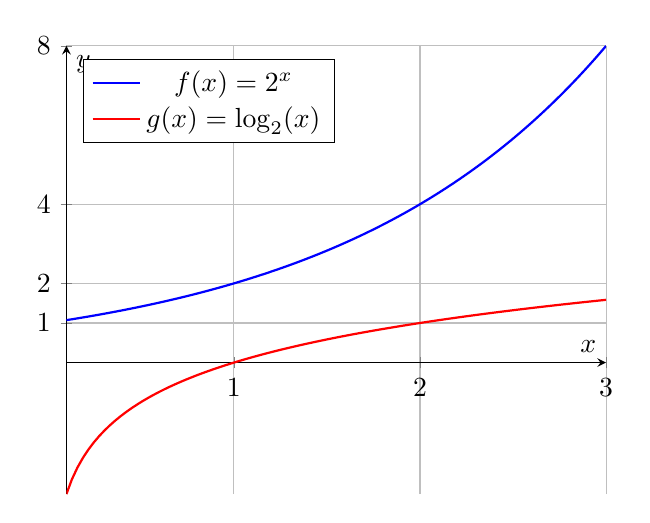
\begin{tikzpicture}[scale=1.0]
    \begin{axis}[
        axis lines = middle,
        xlabel = $x$,
        ylabel = {$y$},
        domain=0.1:3,
        samples=100,
        legend pos=north west,
        xmax=3,
        ymax=8,
        xtick={1, 2, 3},
        ytick={1, 2, 4, 8},
        grid = both,
    ]
    % Plot of f(x) = 2^x
    \addplot [
        color=blue,
        thick,
    ]
    {2^x};
    \addlegendentry{$f(x) = 2^x$}
    
    % Plot of g(x) = \log_2(x)
    \addplot [
        color=red,
        thick,
        domain=0.1:3,
    ]
    {log2(x)};
    \addlegendentry{$g(x) = \log_2(x)$}
    
    \end{axis}
\end{tikzpicture}
\end{center}
} {}{NOTAGS}


 \ex
{\code{FxGGx25x02x04x006}}{50}
{
Graph the function $f(x) = 2^{x+3}$ and $g(x) = \log_2(x) - 3$ on the same axes.

}
{

 

\[ f(x) = 2^{x+3} \]

\[ g(x) = \log_2(x) - 3 \]

To graph these functions, consider the following:

For \( f(x) = 2^{x+3} \):

1. The graph is an exponential function shifted 3 units to the left.
2. Plot points for several values of \( x \) such as \( x = -3, -2, -1, 0, 1, 2 \) and compute \( f(x) \).

For \( g(x) = \log_2(x) - 3 \):

1. The graph is a logarithmic function shifted 3 units down.
2. Plot points for \( x = 2, 4, 8, 16 \), where these values of \( x \) are powers of 2 because \( g(x) \) involves a base 2 logarithm.

Plot all the calculated points on the same set of axes and connect the points smoothly to reflect the behavior of the exponential and logarithmic functions.
} {}{NOTAGS}




 
 \ex
{\code{TESTxxxFxGGx25x04x28x001}}{50}
{
Graph the following function, drawing its asymptotes as dashed lines (also, give the equation of each asymptote). 
$$g(x) = -1 + \dfrac{1}{(x + 2)^3}$$


} {

SOLUTION:

Asymptotes: $x = -2$ (vertical) and $y = -1$ (horizontal).

PUT GRAPH ....

} {}{NOTAGS} 




\subsection{Find Domain \topic{D}} 
 
 
 
 \ex
{\code{FxDx24x12x28x001}}{10}
{
What is the domain of the function
$f(x) = 17x^8 - x^6 +23$?

} {

 

The domain of the function \( f(x) = 17x^8 - x^6 + 23 \) is all real numbers, since it is a polynomial function. Therefore, the domain is:

\[ \text{Domain of } f(x) = (-\infty, \infty) \]
} {}{NOTAGS} 


\ex
{\code{FxDx25x01x22x003}}{10}
{
For $g(u)=\dfrac{u+3}{(u-9)(u+21)}$, for which inputs is $g$ undefined?
}{

 

For \( g(u) = \dfrac{u+3}{(u-9)(u+21)} \), the function is undefined where the denominator is zero:

\[
(u-9)(u+21) = 0
\]

The solutions are:

\[
u-9 = 0 \quad \Rightarrow \quad u = 9
\]

\[
u+21 = 0 \quad \Rightarrow \quad u = -21
\]

Thus, \( g(u) \) is undefined for \( u = 9 \) and \( u = -21 \).
}{}{NOTAGS}

 
 
 
 \ex
{\code{FxDx24x12x28x002}}{10}
{
What is the domain of the following function?

$f(x) = \dfrac{x^2 + 25}{4(x - 3)(2x + 5)}$


} {

 

The domain of the function $f(x) = \dfrac{x^2 + 25}{4(x - 3)(2x + 5)}$ is all real numbers except where the denominator is zero. 

To find the domain, set the denominator equal to zero:

$4(x - 3)(2x + 5) = 0$

This gives the equations:

$x - 3 = 0 \Rightarrow x = 3$

$2x + 5 = 0 \Rightarrow x = -\frac{5}{2}$

Therefore, the domain is:

$x \in \mathbb{R}, \, x \neq 3, \, x \neq -\frac{5}{2}$

In interval notation, this is:

$(-\infty, -\frac{5}{2}) \cup (-\frac{5}{2}, 3) \cup (3, \infty)$
} {}{NOTAGS} 
 
 
 
 \ex
{\code{FxDx24x12x28x003}}{20}
{
 When is the following function undefined?

$f(x) = \dfrac{x^2 + 25}{x^2 -x -20}$


} {

 

The function $f(x) = \dfrac{x^2 + 25}{x^2 - x - 20}$ is undefined when the denominator is zero.

To find when the denominator is zero, solve:

\[ x^2 - x - 20 = 0 \]

This is a quadratic equation, which can be factored as:

\[ (x - 5)(x + 4) = 0 \]

Setting each factor to zero gives the solutions:

\[ x - 5 = 0 \quad \Rightarrow \quad x = 5 \]

\[ x + 4 = 0 \quad \Rightarrow \quad x = -4 \]

Therefore, the function is undefined at:

\[ x = 5 \quad \text{and} \quad x = -4 \]
} {}{NOTAGS} 
 
 
 
 \ex
{\code{FxDx25x01x20x004}}{10}
{
 Let \(f(x) = \dfrac{(-9 + x)(2 + x)}{2(x - 1)(x + 17)}\).

\begin{enumerate}
\item Evaluate \(f(0)\).
\item When is the function undefined?
\end{enumerate}
} {

 

\(f(0) = \dfrac{(-9 + 0)(2 + 0)}{2(0 - 1)(0 + 17)} = \dfrac{(-9)(2)}{2(-1)(17)} = \dfrac{-18}{-34} = \dfrac{9}{17}\)

The function is undefined when the denominator is zero:

\[ 
2(x - 1)(x + 17) = 0 
\]

Solving for \(x\):

1. \(x - 1 = 0 \implies x = 1\)

2. \(x + 17 = 0 \implies x = -17\)

Thus, the function is undefined at \(x = 1\) and \(x = -17\).
} {}{NOTAGS} 
 
 
 
 \ex
{\code{FxDx25x01x20x006}}{10}
{
 Consider the following function: \(f(u) = 10 + \sqrt{u}\).

\begin{enumerate}
\item Evaluate \(f(4)\).
\item What is the domain of \(f\)?
\end{enumerate}
} {

 

\(f(4) = 10 + \sqrt{4} = 10 + 2 = 12\)

The domain of \(f(u)\) is \(u \geq 0\) since the square root function \(\sqrt{u}\) is only defined for non-negative values. 

Therefore, the domain of \(f\) is \([0, \infty)\).
} {}{NOTAGS} 
 
\ex
{\code{FxDx25x01x22x004}}{20}
{
Define $g(u)=\dfrac{-2}{\sqrt{u}}$. Where is $g$ undefined? What is its domain?
}{

 

$g(u) = \dfrac{-2}{\sqrt{u}}$ is undefined when the denominator is zero or when $\sqrt{u}$ is not a real number. 

The function $\sqrt{u}$ is defined for $u > 0$. Hence, $g(u)$ is undefined for $u \leq 0$.

Thus, the domain of $g(u)$ is $u > 0$, which can be written in interval notation as $(0, \infty)$.
}{}{NOTAGS} 
 
 
 \ex
{\code{FxDx25x01x20x001}}{15}
{
 Let \(f(x) = \dfrac{x(9 + 6x)(x - 5)}{4(x - 113)(3x + 66)}\).
\begin{enumerate}
\item Evaluate \(f(0)\).
\item When is the function undefined?
\item What is the domain of the function?
\item Which \(x\) values make \(f(x)=0\)?
\end{enumerate}

} {

 

\[ f(0) = \dfrac{0(9 + 6 \times 0)(0 - 5)}{4(0 - 113)(3 \times 0 + 66)} = 0 \]

The function is undefined when the denominator is zero:
\[ 4(x - 113)(3x + 66) = 0 \]

Setting each factor to zero:
\[ x - 113 = 0 \implies x = 113 \]
\[ 3x + 66 = 0 \implies x = -22 \]

The function is undefined for \( x = 113 \) and \( x = -22 \).

The domain of the function is:
\[ x \in \mathbb{R} \setminus \{113, -22\} \]

To find the \( x \) values that make \( f(x) = 0 \), set the numerator to zero:
\[ x(9 + 6x)(x - 5) = 0 \]

Solving for \( x \):
\[ x = 0 \]
\[ 9 + 6x = 0 \implies x = -\frac{3}{2} \]
\[ x - 5 = 0 \implies x = 5 \]

The \( x \) values that make \( f(x) = 0 \) are:
\[ x = 0, -\frac{3}{2}, 5 \]
} {}{NOTAGS} 
 
 
 
 \ex
{\code{FxDx25x01x20x009}}{50}
{

Let $f(x) = \dfrac{(2x^2 + x)(x - 3)}{(x + 5)(x^2 + x - 2)}$ 

\begin{enumerate}
\item Evaluate $f(3)$, $f(0)$, and $f(-1)$.
\item Determine the values of $x$ for which the function is undefined.

\item Determine the values of $x$ for which the function is defined.
\item What is the domain of the function?

\item For which inputs to the function is the output 0?
\item Find the values of $x$ such that $f(x) = 0$.
\end{enumerate}
} {

 

$f(3) = \dfrac{(2(3)^2 + 3)(3 - 3)}{(3 + 5)((3)^2 + 3 - 2)} = \dfrac{(18 + 3)(0)}{8(9 + 3 - 2)} = 0$

$f(0) = \dfrac{(2(0)^2 + 0)(0 - 3)}{(0 + 5)((0)^2 + 0 - 2)} = \dfrac{0}{5(-2)} = 0$

$f(-1) = \dfrac{(2(-1)^2 + (-1))((-1) - 3)}{((-1) + 5)((-1)^2 - 1 - 2)} = \dfrac{(2 - 1)(-4)}{(4)(-2)} = \dfrac{-4}{-8} = \dfrac{1}{2}$

Values of $x$ for which the function is undefined: set the denominator to zero:

$(x + 5)(x^2 + x - 2) = 0$

$x + 5 = 0 \Rightarrow x = -5$

$x^2 + x - 2 = 0 \Rightarrow (x - 1)(x + 2) = 0 \Rightarrow x = 1, -2$

The function is undefined at $x = -5, 1, -2$.

The function is defined for all other real numbers:

$x \in \mathbb{R} \setminus \{-5, 1, -2\}$

Domain: $(-\infty, -5) \cup (-5, -2) \cup (-2, 1) \cup (1, \infty)$

The output is 0 when the numerator is zero and the denominator is non-zero:

$(2x^2 + x)(x - 3) = 0 \Rightarrow 2x^2 + x = 0$ or $x - 3 = 0$

$2x^2 + x = x(2x + 1) = 0 \Rightarrow x = 0$ or $2x + 1 = 0 \Rightarrow x = -\frac{1}{2}$

$x - 3 = 0 \Rightarrow x = 3$

Check that these values do not make the denominator zero:

For $x = 0$: $(0 + 5)(0^2 + 0 - 2) \neq 0$

For $x = -\frac{1}{2}$: $\left(-\frac{1}{2} + 5\right)\left(\left(-\frac{1}{2}\right)^2 - \frac{1}{2} - 2\right) \neq 0$

For $x = 3$: $(3 + 5)(3^2 + 3 - 2) \neq 0$

Values of $x$ such that $f(x) = 0$: $x = 0, -\frac{1}{2}, 3$
} {}{NOTAGS} 
 
 
  \ex
{\code{FxDx25x01x24x002}}{10}
{
Find the domain of $f(x) = 43 \sqrt{x + 25}$.
} {

 

The domain of the function $f(x) = 43 \sqrt{x + 25}$ requires that the expression inside the square root is non-negative. Hence, we need:

\[ x + 25 \geq 0 \]

Solving this inequality gives:

\[ x \geq -25 \]

Thus, the domain of $f(x)$ is:

\[ \boxed{[-25, \infty)} \]
} {}{NOTAGS} 
 
 
  \ex
{\code{FxDx25x01x24x003}}{10}
{
Find the interval where the function is undefined: $f(x) = 6 \sqrt{5x}$.
} {

 

The function $f(x) = 6 \sqrt{5x}$ is undefined where the expression under the square root is negative. Therefore, we need $5x \geq 0$. 

Solving for $x$, we get:

\[ 5x \geq 0 \]

\[ x \geq 0 \]

Thus, the function is undefined for:

\[ (-\infty, 0) \]
} {}{NOTAGS} 
  
 
 \ex
{\code{FxDx25x01x20x011}}{10}
{
Find the domain of $f(x) = 7 \sqrt{5x + 10}$.
} {

 

The domain of the function $f(x) = 7 \sqrt{5x + 10}$ is determined by the condition inside the square root, which must be non-negative.

\[
5x + 10 \geq 0
\]

Solving this inequality:

\[
5x \geq -10
\]

\[
x \geq -2
\]

Therefore, the domain of $f(x)$ is:

\[
x \in [-2, \infty)
\]
} {}{NOTAGS} 

 \ex
{\code{FxDx25x01x24x001}}{10}
{
Find the domain of $f(x) = 7 \sqrt[3]{5x + 10}$.
} {

 

The function \( f(x) = 7 \sqrt[3]{5x + 10} \) is a cube root function. Cube roots are defined for all real numbers. Therefore, the domain of \( f(x) \) is all real numbers.

The domain is:

\(\mathbb{R}\) 

or in interval notation:

\((-\infty, \infty)\)
} {}{NOTAGS} 
 

  \ex
{\code{FxDx25x01x24x004}}{10}
{
Find the interval where the function is undefined: $f(x) = \sqrt{4x - 6}$.
} {

 

The function $f(x) = \sqrt{4x - 6}$ is undefined when the expression inside the square root is negative. Thus, we need to solve the inequality:

\[
4x - 6 < 0
\]

Solving for $x$, we add 6 to both sides:

\[
4x < 6
\]

Then divide by 4:

\[
x < \frac{3}{2}
\]

Therefore, the function is undefined for the interval:

\[
x \in \left(-\infty, \frac{3}{2}\right)
\]
} {}{NOTAGS}  
 
 
 \ex
{\code{FxDx25x01x20x012}}{10}
{
Find the domain of $g(x) = \dfrac{x^2 + 7}{2x - 4}$.
} {

 

The domain of \( g(x) = \dfrac{x^2 + 7}{2x - 4} \) is determined by the values of \( x \) that do not make the denominator zero.

Set the denominator equal to zero:

\[
2x - 4 = 0
\]

Solving for \( x \):

\[
2x = 4 \implies x = 2
\]

Thus, the function is undefined at \( x = 2 \).

Therefore, the domain of \( g(x) \) is all real numbers except \( x = 2 \).

In interval notation, the domain is:

\[
(-\infty, 2) \cup (2, \infty)
\]
} {}{NOTAGS} 
 
 
 
 \ex
{\code{FxDx25x01x20x013}}{20}
{
 Consider the function $F$ graphed below.
 \begin{figure}[H] 
    \centering
    \includegraphics[scale=.6]{C:/Users/Kerry/Dropbox/MY_STUFF/MY_MATERIALS/Programs/Python/ExerciseManual/ExerciseData/FigsExercises/FxDx25x01x20x013.pdf} 
\end{figure}
 
 
\begin{multicols}{2}
\begin{enumerate}
\item Evaluate $F(-1)$, $F(0)$, $F(1)$.
\item What is the domain and range of $F$?
\end{enumerate}
\end{multicols}

}
{

 

$F(-1) = 2$

$F(0) = 3$

$F(1) = 0$

Domain of $F$: $[-2, 2]$

Range of $F$: $[0, 3]$
} {}{NOTAGS}



 \ex
{\code{FxDx25x02x05x001}}{15}
{
Find the domain of $f(x) = \dfrac{1}{x^2+x-12}$
} {

\vspace{4mm}
SOLUTION:
 Exclude the values where
the denominator is $0$, i.e. the solutions of $x^2+x-12=0$. To solve
this equation, factor: $x^2+x-12 = (x-3)(x+4)=0$, so $x=3$ or
$x=-4$. Therefore the domain of $f$ is $(-\infty -4) \cup (-4,3)\cup
(3, \infty)$.

} {}{NOTAGS} 

 \ex
{\code{FxDx25x02x05x002}}{15}
{
Find the domain of $g(x)=\dfrac{3x+2}{x^2+2x-2}$
} {

\vspace{4mm}
SOLUTION:
Exclude the values where the denominator is $0$, i.e. the
solutions of $x^2+2x-2=0$. To solve this equation, use the quadratic
formula:
$$x = \dfrac{-2 \pm \sqrt{2^2 - 4 \cdot 1\cdot (-2)}}{2\cdot 1} =
\dfrac{-2\pm \sqrt{12}}{2} = -1 \pm \sqrt{3}.$$ Therefore the numbers
$-1+\sqrt{3}$ and $-1-\sqrt{3}$ should be excluded from the domain of
$g$.  Therefore the domain of $g$ is $(-\infty, -1-\sqrt{3})\cup
(-1-\sqrt{3}, -1+\sqrt{3}) \cup (-1+\sqrt{3}, \infty)$
} {}{NOTAGS} 

 \ex
{\code{FxDx25x02x05x003}}{15}
{
Find the domain of $h(x) = \sqrt{3-x}$
} {

\vspace{4mm}
SOLUTION:
For $x$ to be in the domain of $\sqrt{3-x}$, we need the radicand $3-x\ge 0$. Solving this inequality we get $3\ge x$. Therefore the domain is $(-\infty,3]$.

} {}{NOTAGS} 

 \ex
{\code{FxDx25x02x05x004}}{15}
{
Find the domain of $G(x) = \log_5(3x-6)$
} {

\vspace{4mm}
SOLUTION:
For $x$ to be in the domain of $\log_5{3x-6}$, we need $3x-6>0$. Adding $6$ to both sides and dividing by $3$ we get $x> 6/3$, or $x>2$. Therefore the domain is $(2,\infty)$.
} {}{NOTAGS} 





 \ex
{\code{FxDx25x01x24x101}}{5}
{
Let 
\[
h(x)=
\begin{cases}
x - 4, & x < 3,\\
4 - x, & x > 3.
\end{cases}
\]
What is the domain of $h$?
}
{

 

The domain of \( h \) is all real numbers, since \( h(x) \) is defined for every real number \( x \). 

Therefore, the domain of \( h \) is \(\mathbb{R}\).
} {}{NOTAGS}


 \ex
{\code{FxDx25x01x24x102}}{5}
{
Let 
\[
g(x)=
\begin{cases}
4, & x \le 2,\\
\dfrac{3}{x-1}, & x > 2.
\end{cases}
\]
What is the domain of $g$?
}
{

 

The domain of \( g \) is \( (-\infty, 2] \cup (2, \infty) \).
} {}{NOTAGS}

 \ex
{\code{FxDx25x01x24x104}}{5}
{
Let 
\[
f(x)=
\begin{cases}
\dfrac{3}{x-1}, & x \le 2,\\
4, & x > 2.
\end{cases}
\]
What is the domain of $f$?
}
{

 

The domain of \( f \) is \( \{ x \mid x \neq 1 \} \).

This is because:
- For the piece \( \dfrac{3}{x-1} \), \( x \le 2 \), \( x \neq 1 \) (as division by zero is undefined).
- For the piece \( 4 \), \( x > 2 \), all real numbers \( x \) are valid.

Therefore, the domain of \( f \) is \( (-\infty, 1) \cup (1, \infty) \).
} {}{NOTAGS}





\ex
{\code{FxDx25x01x22x010}}{15}
{
Find an example of a rational function whose domain is all real numbers.
}{

 

An example of a rational function whose domain is all real numbers is:

\[ f(x) = \frac{x^2 + 1}{x^2 + 2} \] 

This function is defined for all real numbers since the denominator $x^2 + 2$ never equals zero for any real $x$.
}{}{NOTAGS}


\ex
{\code{CREATIVExxxFxDx25x04x16x001}}{15}
{
Suppose a scientific study defines a function
$f(a)$, where the input ( $a$ ) is the age of a person, and the output is the average height of a person that age.

Decide what the domain should be, giving reasons for your answer (there is not one clear correct answer ...).
}{

 

The domain for the function $f(a)$, where $a$ represents the age of a person and the output is the average height, could be set based on realistic human ages. Generally, $a$ would be a non-negative real number since age cannot be negative. A possible domain could be from birth to an age where human growth typically stops or becomes negligible.

Therefore, we propose:

The domain of $f(a)$ could be $[0, 25] \subset \mathbb{R}$, assuming that the significant, consistent growth in height typically occurs from birth until around age 25. Beyond this age, height changes are usually minimal and related to aging rather than growth.
}{}{NOTAGS}


\subsection{Find Zeroes \topic{Z}} 
 
 
 
 \ex
{\code{FxZx24x12x28x001}}{10}
{
What are the zeroes of the following function?

$f(x) = \dfrac{x^2 + 25}{4(x - 3)(2x + 5)}$

} {

 

The given function is \( f(x) = \dfrac{x^2 + 25}{4(x - 3)(2x + 5)} \).

The zeroes of a function occur where the numerator is equal to zero, since the denominator does not affect the zeroes as long as it does not result in division by zero.

Set the numerator equal to zero:

\[ x^2 + 25 = 0 \]

Solve for \( x \):

\[ x^2 = -25 \]

The equation \( x^2 = -25 \) has no real solutions, since a square of a real number cannot be negative. Therefore, this function has no real zeroes.
} {}{NOTAGS} 
 
 
 
 \ex
{\code{FxZx25x01x20x005}}{10}
{
  Let \(f(x) = \dfrac{(-9 + x)(2 + x)}{2(x - 1)(x + 17)}\).

 For which inputs is the output 0?

}
{

 

The output of the function \( f(x) \) is 0 when the numerator is 0, provided the denominator is not zero. We set the numerator equal to 0:

\[
(-9 + x)(2 + x) = 0
\]

Solving for \( x \):

1. \(-9 + x = 0\)

   \[
   x = 9
   \]

2. \(2 + x = 0\)

   \[
   x = -2
   \]

The values \( x = 9 \) and \( x = -2 \) are solutions if they do not make the denominator zero. We need to check these values in the denominator:

\[
2(x - 1)(x + 17) \neq 0
\]

Checking \( x = 9 \):

\[
2(9 - 1)(9 + 17) = 2(8)(26) \neq 0
\]

Checking \( x = -2 \):

\[
2(-2 - 1)(-2 + 17) = 2(-3)(15) \neq 0
\]

Both \( x = 9 \) and \( x = -2 \) do not make the denominator zero. Therefore, the inputs for which the output is 0 are:

\[
x = 9 \quad \text{and} \quad x = -2
\]
} {}{NOTAGS}




\ex
{\code{FxZx25x01x22x102}}{15}
{
Consider $g(u)=\dfrac{u+3}{(u-9)(u+21)}$.
\begin{multicols}{2}
\begin{enumerate}
\item Evaluate $g(0)$.
\item For which inputs is $g(u)=0$?
\end{enumerate}
\end{multicols}
}{

 

$g(0) = \dfrac{0+3}{(0-9)(0+21)} = \dfrac{3}{(-9)(21)} = \dfrac{3}{-189} = -\dfrac{1}{63}$

To find when $g(u) = 0$, solve $\dfrac{u+3}{(u-9)(u+21)} = 0$. This occurs when $u+3 = 0$, so:

$u + 3 = 0 \implies u = -3$
}{}{NOTAGS}



\ex
{\code{FxZx25x01x22x011}}{15}
{
Find an example of a rational function whose output is never zero.
}{

 

Let \( f(x) = \frac{1}{x} \).

The output of this rational function is never zero since \(\frac{1}{x} \neq 0 \) for any value of \( x \neq 0 \).
}{}{NOTAGS}





  \ex
{\code{FxZx25x02x18x001}}{15}
{
For each function, find the zeroes and their multiplicities.  

\begin{multicols}{2}
\begin{enumerate}
\item $f(x) = (x - 3)^2(x + 1)^4$

\item $g(x) = (x + 4)(x - 12)^3(x - 1)$

\end{enumerate}
\end{multicols}

}
{

 

$f(x) = (x - 3)^2(x + 1)^4$

Zeroes:

- $x = 3$, multiplicity 2.
- $x = -1$, multiplicity 4.

$g(x) = (x + 4)(x - 12)^3(x - 1)$

Zeroes:

- $x = -4$, multiplicity 1.
- $x = 12$, multiplicity 3.
- $x = 1$, multiplicity 1.
} {}{NOTAGS} 


  \ex
{\code{FxZx25x02x18x002}}{15}
{
For each function, find the zeroes and their multiplicities.   

\begin{multicols}{2}
\begin{enumerate}
\item $f(x) = (2x - 1)^3 (x + 7)$

\item $h(x) = (4x + 5)^2 (7x)^5$

\end{enumerate}
\end{multicols}

}
{

 

For $f(x) = (2x - 1)^3(x + 7)$:

Zeroes:

- Set $2x - 1 = 0$: 

  $2x = 1 \implies x = \frac{1}{2}$ 

  Multiplicity: 3

- Set $x + 7 = 0$: 

  $x = -7$ 

  Multiplicity: 1

For $h(x) = (4x + 5)^2(7x)^5$:

Zeroes:

- Set $4x + 5 = 0$: 

  $4x = -5 \implies x = -\frac{5}{4}$ 

  Multiplicity: 2

- Set $7x = 0$: 

  $x = 0$ 

  Multiplicity: 5
} {}{NOTAGS} 


  \ex
{\code{FxZx25x02x19x001}}{15}
{
Find the roots and their multiplicities for the function
$f(x) = 5x^5 - 45x^3$   

}
{

 

The function given is:

\[ f(x) = 5x^5 - 45x^3 \]

First, factor out the greatest common factor:

\[ f(x) = 5x^3(x^2 - 9) \]

Notice that \(x^2 - 9\) can be further factored using the difference of squares:

\[ x^2 - 9 = (x - 3)(x + 3) \]

Thus, we can write:

\[ f(x) = 5x^3(x - 3)(x + 3) \]

Now, find the roots by setting \(f(x) = 0\):

1. \(5x^3 = 0 \Rightarrow x = 0\) (multiplicity 3)
2. \(x - 3 = 0 \Rightarrow x = 3\) (multiplicity 1)
3. \(x + 3 = 0 \Rightarrow x = -3\) (multiplicity 1)

The roots are:

- \(x = 0\) with multiplicity 3
- \(x = 3\) with multiplicity 1
- \(x = -3\) with multiplicity 1
} {}{NOTAGS} 




  \ex
{\code{TESTxFxZx25x02x18x001}}{15}
{
For each function, find the zeroes and their multiplicities.   

\begin{multicols}{2}
\begin{enumerate}
\item $f(x) = (x - 7)^6 (x + 5)^9$

\item $h(x) = (4x + 12)^2 (x^7)$

\end{enumerate}
\end{multicols}

}
{

 

For the function $f(x) = (x - 7)^6 (x + 5)^9$, the zeroes and their multiplicities are:

Zero at $x = 7$ with multiplicity 6.

Zero at $x = -5$ with multiplicity 9.

For the function $h(x) = (4x + 12)^2 (x^7)$, the zeroes and their multiplicities are:

Zero at $x = -3$ with multiplicity 2 (since $4x + 12 = 0 \Rightarrow x = -3$).

Zero at $x = 0$ with multiplicity 7.
} {}{NOTAGS} 







\subsection{Mixed: Domain and Zeroes \topic{DZ}} 



 \ex
{\code{TESTxFxDZx25x02x13x001}}{15}
{
 Let \(f(x) = \dfrac{x^2 - 3x - 4}{-2(x + 10)(5x - 10)}\)
\begin{enumerate}
\item When is the function undefined?
\item What is the domain of the function?
\item Evaluate \(f(0)\).
\item Which \(x\) values make \(f(x)=0\)?
\end{enumerate}

} {

 

1. The function \(f(x)\) is undefined when the denominator is zero. Solve:

\((-2)(x + 10)(5x - 10) = 0\)

This gives \(x + 10 = 0\) or \(5x - 10 = 0\).

Hence, \(x = -10\) or \(x = 2\).

2. The domain of \(f(x)\) is all real numbers except \(x = -10\) and \(x = 2\). In interval notation, the domain is:

\((-\infty, -10) \cup (-10, 2) \cup (2, \infty)\)

3. Evaluate \(f(0)\):

\[f(0) = \frac{0^2 - 3 \times 0 - 4}{-2(0 + 10)(5 \times 0 - 10)} = \frac{-4}{-2(10)(-10)} = \frac{-4}{200} = -\frac{1}{50}\]

4. To find the values of \(x\) that make \(f(x)=0\), set the numerator equal to zero:

\[x^2 - 3x - 4 = 0\]

Factor:

\((x - 4)(x + 1) = 0\)

Thus, \(x = 4\) or \(x = -1\).

The \(x\) values that make \(f(x) = 0\) are \(x = 4\) and \(x = -1\).
} {}{NOTAGS} 


 \ex
{\code{FxDZx25x09x15x001}}{25}
{
 Let \(f(x) = \dfrac{x^2 - 25}{-2(x + 3)(4x - 12)}\)
\begin{enumerate}
\item When is the function undefined?
\item What is the domain of the function?
\item Evaluate \(f(0)\).
\item Which \(x\) values make \(f(x)=0\)?
\end{enumerate}

} {

SOLUTION:

a) Undefined when $-2(x + 3)(4x - 12) = 0$ so for either $(x + 3) = 0$ or
$(4x - 12) = 0$, so for $x = -3, 3$

b) All reals except $-3$ and $3$.

c) $f(0) = \dfrac{(0)^2 - 25}{-2( (0) + 3)(4(0) - 12)} = 
\dfrac{- 25}{-2(3)(- 12)} = -\dfrac{25}{72}$

d) The output is zero when $x^2 - 25 = 0$. 
To solve, add 25 to both sides to get: $x^2 = 25$, whose solutions 
are $x = -5, 5$.

} {}{type: TEST} 





\ex
{\code{GPTx26x02x20x007}}{25}
{
Let $f(x)=\dfrac{x^2-16}{(x-4)(x+2)}$.

\begin{enumerate}
\item When is the function undefined?
\item What is the domain?
\item Evaluate $f(0)$.
\item For which $x$ does $f(x)=0$?
\end{enumerate}
}
{

 

a) Denominator zero when $x=4$ or $x=-2$, so undefined at $4, -2$.

b) Domain: all real numbers except $x=4,-2$.

c) $f(0)=\frac{-16}{(-4)(2)}=\frac{-16}{-8}=2$.

d)
$f(x)=0$ when numerator $x^2 - 16 = 0$, so solve to see 
$x=\pm4$. But $x=4$ undefined $\rightarrow$ only $x=-4$.
} {}{type: TEST}



 \ex
{\code{TESTxxxFxDZx25x04x28x001}}{25}
{
 Let \(f(x) = \dfrac{x^2 + 7}{3x^2 - 2x - 1}\).
\begin{enumerate}
\item What is the domain?
\item What are the vertical asymptotes?
\item What is the horizontal asymptote?
\end{enumerate}

} {

SOLUTION:

Factor bottom: $3x^2 - 2x - 1 = (3x +1)(x -1)$, so it is zero when
$x = -\frac{1}{3}, 1$.

\begin{enumerate}
\item Domain: All reals except $-\frac{1}{3}, 1$
\item Vertical asymptotes: $x = -\frac{1}{3}$ and $x = 1$
\item Horizontal asymptote: $y = \frac{1}{3}$ (since the ratio of the leading terms is
$\frac{x^2}{3x^2} = \frac{1}{3}$)
\end{enumerate}


} {}{NOTAGS} 



 \ex
{\code{TESTxxxFxDZx26x05x01x004}}{25}
{
 Let \(f(x) = \dfrac{4x^2 + 7}{x^2 - x - 12}\).
\begin{enumerate}
\item What is the domain?
\item What are the vertical asymptotes?
\item What is the horizontal asymptote?
\end{enumerate}

} {



} {}{NOTAGS} 




\subsection{End Behavior and Basic Limits \topic{LIM}} 


\ex
{\code{FxLIMx25x02x18x001}}{15}
{
Determine the end behavior of the functions.

\begin{multicols}{2}
\begin{enumerate}
\item  $g(x) = 3x^5$
\item $f(x) = -7x^5$

\end{enumerate}
\end{multicols}
}{

 

\[
\text{For } g(x) = 3x^5:
\]

- \text{As } $x \to \infty, \ g(x) = 3x^5 \to \infty$

- \text{As } $x \to -\infty, \ g(x) = 3x^5 \to -\infty$

\[
\text{For } f(x) = -7x^5:
\]

- \text{As } $x \to \infty, \ f(x) = -7x^5 \to -\infty$

- \text{As } $x \to -\infty, \ f(x) = -7x^5 \to \infty$
}{}{NOTAGS}


\ex
{\code{FxLIMx25x02x18x002}}{15}
{
Determine the end behavior of the functions.

\begin{multicols}{2}
\begin{enumerate}
\item  $g(x) = 9x^4$
\item $f(x) = -5x^6$

\end{enumerate}
\end{multicols}
}{

 

For the function $g(x) = 9x^4$, as $x \to \infty$, $g(x) \to \infty$ and as $x \to -\infty$, $g(x) \to \infty$.

For the function $f(x) = -5x^6$, as $x \to \infty$, $f(x) \to -\infty$ and as $x \to -\infty$, $f(x) \to -\infty$.
}{}{NOTAGS}




\ex
{\code{FxLIMx25x02x18x004}}{15}
{

Determine $\lim_{x \rightarrow \infty} f(x)$ for each function.

\begin{multicols}{2}
\begin{enumerate}
\item  $f(x) = 9x^4$
\item $f(x) =  15x^3$

\end{enumerate}
\end{multicols}
}{

 

\[
\lim_{x \rightarrow \infty} 9x^4 = \infty
\]

\[
\lim_{x \rightarrow \infty} 15x^3 = \infty
\]
}{}{NOTAGS}


\ex
{\code{FxLIMx25x02x18x005}}{15}
{

Determine $\lim_{x \rightarrow -\infty} g(x)$ for each function.

\begin{multicols}{2}
\begin{enumerate}
\item  $g(x) = 3x^5$
\item $g(x) =  4x^6$

\end{enumerate}
\end{multicols}
}{

 

$\lim_{x \rightarrow -\infty} g(x) = \lim_{x \rightarrow -\infty} 3x^5 = -\infty$

$\lim_{x \rightarrow -\infty} g(x) = \lim_{x \rightarrow -\infty} 4x^6 = \infty$
}{}{NOTAGS}



\ex
{\code{FxLIMx25x01x22x001}}{15}
{
Determine the end behavior of the function \(g(x) = 3x^5 + 7x^2 - x + 12\).
}{

 

The end behavior of the function \(g(x) = 3x^5 + 7x^2 - x + 12\) is determined by the leading term \(3x^5\), as this term dominates the behavior of the polynomial for very large and very small values of \(x\).

- As \(x \to \infty\), \(3x^5 \to \infty\), so \(g(x) \to \infty\).

- As \(x \to -\infty\), \(3x^5 \to -\infty\), so \(g(x) \to -\infty\).

Thus, the end behavior of the function is:

\junk{
\[
\begin{aligned}
&\text{As } x \to \infty, \, g(x) \to \infty. \\
&\text{As } x \to -\infty, \, g(x) \to -\infty.
\end{aligned}
\]
}
}{}{NOTAGS}


\ex
{\code{FxLIMx25x02x19x002}}{15}
{
Determine the end behavior of the function \(f(x) = 3x^3 + 7x^4 - 17x\).
}{

 

The end behavior of the function \(f(x) = 3x^3 + 7x^4 - 17x\) is determined by the term with the highest degree, which is \(7x^4\).

As \(x \to \infty\), \(f(x) \to 7x^4 \to \infty\).

As \(x \to -\infty\), \(f(x) \to 7x^4 \to \infty\).

Therefore, the end behavior is:


\begin{align*}
\text{As } x \to \infty, & \quad f(x) \to \infty, \\
\text{As } x \to -\infty, & \quad f(x) \to \infty.
\end{align*}

}{}{NOTAGS}

\ex
{\code{FxLIMx25x02x19x004}}{15}
{
Determine the end behavior of the function \(h(x) = 3x^7 + 7x^3 - 10x^7\).
}{

 

The given function is 

\[ 
h(x) = 3x^7 + 7x^3 - 10x^7 
\]

Simplify the expression:

\[ 
h(x) = (3x^7 - 10x^7) + 7x^3 = -7x^7 + 7x^3 
\]

The term that determines the end behavior is the highest-degree term, \(-7x^7\).

As \(x \to \infty\), \(-7x^7 \to -\infty\).

As \(x \to -\infty\), \(-7x^7 \to \infty\).

Thus, the end behavior of the function is:


\begin{align*}
\text{As } x \to \infty, & \quad h(x) \to -\infty, \\
\text{As } x \to -\infty, & \quad h(x) \to \infty.
\end{align*}

}{}{NOTAGS}


\ex
{\code{HWxFxLIMx25x02x18x003}}{15}
{
Determine the end behavior of the functions.

\begin{multicols}{2}
\begin{enumerate}
\item  $g(x) = -90x^2$
\item $f(x) = 5x^3$

\end{enumerate}
\end{multicols}
}{

 

$g(x) = -90x^2$: As $x \to \infty$, $g(x) \to -\infty$ and as $x \to -\infty$, $g(x) \to -\infty$.

$f(x) = 5x^3$: As $x \to \infty$, $f(x) \to \infty$ and as $x \to -\infty$, $f(x) \to -\infty$.
}{}{type: HW}


\ex
{\code{HWxFxLIMx25x02x19x003}}{15}
{
Determine the end behavior of the function \(f(x) = 3x^3 + 7x^4 - 17x\).
}{

 

The end behavior of a polynomial function is determined by the term with the highest degree. In the function \(f(x) = 3x^3 + 7x^4 - 17x\), the term with the highest degree is \(7x^4\).

Thus, the end behavior is similar to the end behavior of \(y = 7x^4\).

For \(y = 7x^4\):

- As \(x \to \infty\), \(y \to \infty\).
- As \(x \to -\infty\), \(y \to \infty\).

Therefore, the end behavior of the function \(f(x)\) is:

As \(x \to \infty\), \(f(x) \to \infty\).

As \(x \to -\infty\), \(f(x) \to \infty\).
}{}{type: HW}



\ex
{\code{TESTxFxLIMx25x02x19x007}}{15}
{
Determine the end behavior of the function \(f(x) = 3x^5 + 7x^2 - 17x^3\).
}{

SOLUTION:

The leading term is $3x^5$, which has a \emph{positive} coefficient,
and an \emph{odd} exponent, thus:
\begin{itemize}

\item As $x \rightarrow +\infty$, we have $f \rightarrow +\infty$

\item As $x \rightarrow -\infty$, we have $f \rightarrow -\infty$

\end{itemize}

}{}{type: TEST}




\ex
{\code{TESTxFxLIMx25x02x18x001}}{25}
{
Determine the end behavior of the functions.

\begin{multicols}{2}
\begin{enumerate}
\item  $h(x) = 10x^3$
\item $f(x) = -5x^4$

\end{enumerate}
\end{multicols}
}{

SOLUTION:

As $x \rightarrow + \infty, \ h(x) \rightarrow + \infty$ (by test value: $h(1) = 10 > 0$)

As $x \rightarrow - \infty, \ h(x) \rightarrow - \infty$ (by test value: $h(-1) = -10 < 0$)

As $x \rightarrow + \infty, \ f(x) \rightarrow - \infty$ (since exponent even and coefficient negative)


As $x \rightarrow - \infty, \ f(x) \rightarrow - \infty$ (since exponent even and coefficient negative)


}{}{type: TEST}


\ex
{\code{TESTxFxLIMx26x03x22x001}}{25}
{
Determine the end behavior of the functions.

\begin{multicols}{2}
\begin{enumerate}

\item $g(x) = -3x^6$
\item  $h(x) = 12x^7$


\end{enumerate}
\end{multicols}
}{

SOLUTION:

As $x \rightarrow + \infty, \ g(x) \rightarrow - \infty$ (since exponent even and coefficient negative)


As $x \rightarrow - \infty, \ g(x) \rightarrow - \infty$ (since exponent even and coefficient negative)



As $x \rightarrow + \infty, \ h(x) \rightarrow + \infty$ (by test value: $h(1) = 12 > 0$)

As $x \rightarrow - \infty, \ h(x) \rightarrow - \infty$ (by test value: $h(-1) = -12 < 0$)


}{}{type: TEST}


\ex
{\code{TESTxFxLIMx26x05x01x001}}{25}
{
Determine the end behavior of the functions.

\begin{multicols}{2}
\begin{enumerate}

\item $g(x) = -3x^8$
\item  $h(x) = 4x^3 + 10x^7$


\end{enumerate}
\end{multicols}
}{

SOLUTION:

As $x \rightarrow + \infty, \ g(x) \rightarrow - \infty$ (since exponent even and coefficient negative)


As $x \rightarrow - \infty, \ g(x) \rightarrow - \infty$ (since exponent even and coefficient negative)


As $x \rightarrow + \infty, \ h(x) \rightarrow + \infty$ (by test value in leading term: $10(1)^7 = 10 > 0$)

As $x \rightarrow - \infty, \ h(x) \rightarrow - \infty$ (by test value in leading term: $10(-1)^7 = -10 < 0$)


}{}{type: TEST}



\ex
{\code{TESTxFxLIMx25x02x18x002}}{15}
{

Determine $\lim_{x \rightarrow \infty} f(x)$ for each function.

\begin{multicols}{2}
\begin{enumerate}
\item  $f(x) = 9x^3$
\item $f(x) =  -x^5$

\end{enumerate}
\end{multicols}
}{

 

\[
\lim_{x \rightarrow \infty} 9x^3 = \infty
\]

\[
\lim_{x \rightarrow \infty} -x^5 = -\infty
\]
}{}{NOTAGS}




\subsection{Arithmetic On Functions \topic{AR}} 
 
 
 
 \ex
{\code{FxARx25x01x20x010}}{10}
{
Let $f(x)=x^3$ and $g(x)=x-1$.
\begin{multicols}{2}
\begin{enumerate}
\item Find $(f+g)(-3)$
\item Find $(f-g)(-3)$

\item Find $(f*g)(-3)$
\item Find $\Bigl(\dfrac{f}{g}\Bigr)(-3)$
\end{enumerate}
\end{multicols}
}
{

 

$(f+g)(x) = f(x) + g(x) = x^3 + (x - 1) = x^3 + x - 1$

$(f+g)(-3) = (-3)^3 + (-3) - 1 = -27 - 3 - 1 = -31$

$(f-g)(x) = f(x) - g(x) = x^3 - (x - 1) = x^3 - x + 1$

$(f-g)(-3) = (-3)^3 - (-3) + 1 = -27 + 3 + 1 = -23$

$(f \cdot g)(x) = f(x) \cdot g(x) = x^3 \cdot (x - 1) = x^4 - x^3$

$(f \cdot g)(-3) = (-3)^4 - (-3)^3 = 81 + 27 = 108$

$\left(\frac{f}{g}\right)(x) = \frac{f(x)}{g(x)} = \frac{x^3}{x-1}$

$\left(\frac{f}{g}\right)(-3) = \frac{(-3)^3}{-3-1} = \frac{-27}{-4} = \frac{27}{4}$
} {}{NOTAGS}


 \ex
{\code{FxARx25x01x24x001}}{20}
{
Let $f(x)=x^3$ and $g(x)=x-1$.
For each of the following, find the simplified and expanded form.
\begin{multicols}{2}
\begin{enumerate}
\item $(f+g)$
\item $(f-g)$

\item $(f*g)$
\end{enumerate}
\end{multicols}
}
{

 

\((f+g)(x) = f(x) + g(x) = x^3 + (x-1) = x^3 + x - 1\)

\((f-g)(x) = f(x) - g(x) = x^3 - (x-1) = x^3 - x + 1\)

\((f \cdot g)(x) = f(x) \cdot g(x) = x^3 \cdot (x-1) = x^3 \cdot x - x^3 = x^4 - x^3\)
} {}{NOTAGS}


 \ex
{\code{FxARx25x01x24x002}}{20}
{
Let $f(x)=\dfrac{1}{x^3}$ and $g(x)=\sqrt{x+1}$.
Find the domain of each of the following.
\begin{multicols}{2}
\begin{enumerate}
\item $(f+g)$
\item $(f-g)$

\item $(f*g)$

\item
$\Bigl(\dfrac{f}{g}\Bigr)$
\end{enumerate}
\end{multicols}
}
{

 

The function \( f(x) = \dfrac{1}{x^3} \) is defined for \( x \neq 0 \). The function \( g(x) = \sqrt{x+1} \) is defined for \( x \geq -1 \).

1. \((f+g)(x)\)

The domain of \( (f+g)(x) \) is the intersection of the domains of \( f(x) \) and \( g(x) \).

\[
-1 \leq x < 0 \quad \text{or} \quad x > 0
\]

2. \((f-g)(x)\)

The domain of \( (f-g)(x) \) is the same as that of \( (f+g)(x) \).

\[
-1 \leq x < 0 \quad \text{or} \quad x > 0
\]

3. \((f \cdot g)(x)\)

The domain of \( (f \cdot g)(x) \) is the intersection of the domains of \( f(x) \) and \( g(x) \).

\[
-1 \leq x < 0 \quad \text{or} \quad x > 0
\]

4. \(\left(\dfrac{f}{g}\right)(x)\)

The domain of \(\left(\dfrac{f}{g}\right)(x)\) is the intersection of the domains of \( f(x) \) and \( g(x) \), excluding where \( g(x) = 0 \). Since \( g(x) = \sqrt{x+1} \), \( g(x) = 0 \) at \( x = -1 \).

\[
-1 < x < 0 \quad \text{or} \quad x > 0
\]
} {}{NOTAGS}


 \ex
{\code{FxARx25x01x24x003}}{20}
{
Find an example of function $f$ and $g$ so that 
$\Bigl(\dfrac{f}{g}\Bigr)$ is defined everywhere.
}
{

 

Let $f(x) = x^2 + 1$ and $g(x) = x^2 + 1$. Then $\Bigl(\dfrac{f}{g}\Bigr)(x) = \dfrac{x^2 + 1}{x^2 + 1} = 1$ for all $x \in \mathbb{R}$, which is defined everywhere since $g(x) \neq 0$ for all real $x$.
} {}{NOTAGS}



 \ex
{\code{TESTxFxARx25x02x14x001}}{15}
{
Let $f(x)=\dfrac{2}{x - 5}$ and $g(x)=\sqrt{2x - 4}$.
Find the domain of each of the following.
\begin{enumerate}
\item $(f+g)$
\item $(f-g)$

\item $(f*g)$

\end{enumerate}
}
{

 

The domain of $f(x)=\dfrac{2}{x - 5}$ is all real numbers except $x = 5$.

The domain of $g(x)=\sqrt{2x - 4}$ is determined by the condition $2x - 4 \geq 0$, which simplifies to $x \geq 2$.

Thus, the domain of any combination of $f$ and $g$ is the intersection of their domains: $x \geq 2$ and $x \neq 5$. This intersection can be written as $[2, 5) \cup (5, \infty)$.

\begin{enumerate}
\item The domain of $(f+g)(x)$ is $[2, 5) \cup (5, \infty)$.

\item The domain of $(f-g)(x)$ is $[2, 5) \cup (5, \infty)$.

\item The domain of $(f \cdot g)(x)$ is $[2, 5) \cup (5, \infty)$.
\end{enumerate}
} {}{NOTAGS}


 \ex
{\code{FxARx25x09x15x001}}{15}
{
Let $f(x)=\dfrac{2}{3x - 5}$ and $g(x)=\sqrt{5x - 20}$.
Find the domain of each of the following.
\begin{multicols}{3}
\begin{enumerate}
\item $(f+g)$
\item $(f-g)$

\item $(f*g)$

\end{enumerate}
\end{multicols}
}
{

SOLUTION:

All 3 functions have the same domain.

First, the domain of $f$: Undefined when $3x - 5 = 0$, so when $x = \frac{5}{3}$.

Second, the domain of $g$: Need $5x - 20 \ge 0$, so when $x \ge 4$.

Answer: Take only the numbers in both domains.  Since $\frac{5}{3} < 4$,
we just take what is allowed by $g$ (i.e. $x \ge 4$) and that exludes the one undefined value for $f$ (i.e. $\frac{5}{3}$) so the domain of each of the 3 functions is: All real $x$ such that $x \ge 4$.


} {}{type: TEST}



 \ex
{\code{TESTxFxARx25x02x14x002}}{15}
{
Let $f(x)= x^2 - 1$ and $g(x)=\dfrac{2}{x}$.
Find the domain of each of the following.
\begin{multicols}{2}
\begin{enumerate}
\item $\dfrac{f}{g}$

\item $\dfrac{g}{f}$

\end{enumerate}
\end{multicols}
}
{

 

\item \(\frac{f}{g}(x) = \frac{x^2 - 1}{\frac{2}{x}} = \frac{x(x^2 - 1)}{2}\)

The domain requires \(g(x) \neq 0\) and for \(\frac{f}{g}\) itself to be defined:

1. \(g(x) \neq 0 \Rightarrow \frac{2}{x} \neq 0 \Rightarrow x \neq 0\).

Since the denominator after simplification is a constant (\(2\)), there are no additional restrictions.

Thus, the domain is \(x \in \mathbb{R} \setminus \{0\}\).

\item \(\frac{g}{f}(x) = \frac{\frac{2}{x}}{x^2 - 1} = \frac{2}{x(x^2 - 1)}\)

The domain requires \(f(x) \neq 0\) and \(x \neq 0\):

1. \(f(x) \neq 0 \Rightarrow x^2 - 1 \neq 0 \Rightarrow x \neq \pm 1\).
2. \(x \neq 0\).

Thus, the domain is \(x \in \mathbb{R} \setminus \{-1, 0, 1\}\).
} {}{NOTAGS}



\ex
{\code{GPTx26x02x20x009}}{30}
{
Let $f(x)=x^2-9$ and $g(x)=\dfrac{2}{x-2}$.
Find the domain of:

\begin{multicols}{2}
\begin{enumerate}
\item $\dfrac{f}{g}$
\item $\dfrac{g}{f}$
\end{enumerate}
\end{multicols}

}
{

 

$g$ undefined at $x=2$.
$f=0$ at $x=\pm3$.

(a) $\frac{f}{g}$: denominator $g(x)$ is never zero, but $g$ is undefined when $x = 2$. So domain: all reals except 2.

(b) $\frac{g}{f}$: denominator $f(x)$ is zero when $x= \pm3$, and $g$ is undefined when $x = 2$, so domain: all reals except $-3,2,3$.
} {}{type: TEST}



 \ex
{\code{FxARx25x09x15x002}}{15}
{
Let $f(x)= x^2 - 4$ and $g(x)=\dfrac{3}{x + 1}$.
Find the domain of each of the following.
\begin{multicols}{2}
\begin{enumerate}
\item $\dfrac{f}{g}$

\item $\dfrac{g}{f}$

\end{enumerate}
\end{multicols}
}
{

SOLUTION:

First note that the domain of $f$: All reals; and domain of $g$: All reals except $-1$.
Also, in both (a) and (b), note that we at least need both $f$ and $g$ defined, so consider: All reals except $-1$.  Now have the extra worry about division by zero in each case. 

\vspace{3mm}
a) The bottom function $g$ can be undefined but never zero, so the domain is:
All reals except $-1$.

\vspace{3mm}
b) We check when the bottom function can equal zero, that is
$x^2 - 4 = 0$.  Solve that by adding 4 to both sides to get $x^2 = 4$, so
$x = -2, 2$.  Thus in this case the function is undefined for $-2, -1, 2$, so the domain is:
All reals except $-2, -1, 2$.


} {}{type: TEST}




\ex
{\code{GPTx26x02x20x008}}{30}
{
Let $f(x)=\dfrac{3}{x-1}$ and $g(x)=\sqrt{2x-6}$.
Find the domain of:

\begin{multicols}{3}
\begin{enumerate}
\item $(f+g)$
\item $(f-g)$
\item $(f\cdot g)$
\end{enumerate}
\end{multicols}
}
{

 

$f$ undefined at $x=1$.
$g$ requires $2x-6\ge0 \Rightarrow x\ge3$.

Intersection $\rightarrow$ $x\ge3$.

Domain for all three: $[3,\infty)$.
} {}{type: TEST}


%BREAK
\end{itemize}
\begin{itemize}


\subsection{Composition Of Functions \topic{CP}} 
 
 
  \ex
{\code{FxCPx25x01x24x001}}{20}
{
  If the order is reversed
when composing two
functions, can the result
ever be the same as the
answer in the original order
of the composition? If yes,
give an example. If no,
explain why not.
} {

 

Yes, the order can be reversed and still yield the same result in certain cases.

Consider the functions $f(x) = x + 1$ and $g(x) = x - 1$.

Compute the compositions:

1. $f(g(x)) = f(x - 1) = (x - 1) + 1 = x$.

2. $g(f(x)) = g(x + 1) = (x + 1) - 1 = x$.

In this example, $f(g(x)) = g(f(x)) = x$, which shows that it is possible for the order reversal to yield the same result.
} {}{NOTAGS} 
 
 

 
 
 
 \ex
{\code{FxCPx25x01x20x012}}{10}
{
Let $f(x)=2x$ and $g(x)=x+10$.
\begin{multicols}{2}
\begin{enumerate}
\item Find $(f\circ g)(5)$
\item Find $g(f(5))$

\item Find $f(f(5))$
\item Find $(g\circ g)(5)$
\end{enumerate}
\end{multicols}
} {

 

$(f \circ g)(5) = f(g(5)) = f(5 + 10) = f(15) = 2 \times 15 = 30$

$g(f(5)) = g(2 \times 5) = g(10) = 10 + 10 = 20$

$f(f(5)) = f(2 \times 5) = f(10) = 2 \times 10 = 20$

$(g \circ g)(5) = g(g(5)) = g(5 + 10) = g(15) = 15 + 10 = 25$
} {}{NOTAGS} 
 
 
 
 \ex
{\code{FxCPx25x02x05x001}}{20}
{
Given $f(x) = 2x+1$ and $g(x)=x^2+3$, find and simplify the following.
\begin{multicols}{2}
\begin{enumerate}

\item 
$(f\circ g)(3)$ 

\item
$(f\circ g)(x)$ 

\item
$(g\circ f)(x)$ 

\item
$(f\circ g \circ f )(x)$


\end{enumerate}
\end{multicols}
} {

\vspace{4mm}
SOLUTIONS:

\begin{enumerate}

\item
 $(f\circ g)(3) = f(g(3))
= f(12) = 25$

\item
$(f\circ g)(x) = f(g(x)) = f(x^2+3) = 2(x^2+3)+1 =
2x^2+7$

\item
$(g\circ f)(x) = g(f(x)) = g(2x+1) = (2x+1)^2 +3 = 4x^2+4x+4 =
4(x^2+x+1)$

\item
$(f\circ g\circ f)(x) = f(g(f(x))) = f(g(2x+1)) = f((2x+1)^2 +
3) = 2 ((2x+1)^2 + 3) + 1 = 8x^2+8x+9$ 

\end{enumerate}

} {}{NOTAGS}  



\ex
{\code{GPTx26x02x20x010}}{30}
{
Let $f(x)=3x+2$ and $g(x)=4x-5$.

\begin{enumerate}
\item Find $(f\circ g)(2)$.
\item Simplify $f(g(x))$.
\item Simplify $(g\circ f)(x)$.
\end{enumerate}
}
{

 

(a) $(f\circ g)(2) = f(g(2)) = f(3) = 11$


(b)
$f(g(x))=3(4x-5)+2=12x-15+2=12x-13$.

(c)
$g(f(x))=4(3x+2)-5=12x+8-5=12x+3$.

} {}{type: TEST}



 \ex
{\code{FxCPx25x10x27x001}}{35}
{
Let $f(x) = -9 - 3x$ and $g(x)=2 + x^3$.
\begin{multicols}{2}
\begin{enumerate}

\item Evaluate
$(g \circ f)(-2)$ 

\item Simplify
$(f\circ g)(x)$ 

\end{enumerate}
\end{multicols}
} {

 

\((g \circ f)(-2) = g(f(-2))\)

First, find \(f(-2)\):

\[ f(-2) = -9 - 3(-2) = -9 + 6 = -3 \]

Now, substitute into \(g(x)\):

\[ g(-3) = 2 + (-3)^3 = 2 - 27 = -25 \]

Thus, \((g \circ f)(-2) = -25\).

\vspace{10pt}

\((f \circ g)(x) = f(g(x))\)

Substitute \(g(x)\) into \(f(x)\):

\[ g(x) = 2 + x^3 \]

\[ f(g(x)) = f(2 + x^3) \]

\[ = -9 - 3(2 + x^3) \]

\[ = -9 - 6 - 3x^3 \]

\[ = -15 - 3x^3 \]

Thus, \((f \circ g)(x) = -3x^3 - 15\).
} {}{type: TEST}  



 \ex
{\code{FxCPx25x11x05x004}}{35}
{
Let $f(x) = 5 - 2x$ and $g(x)=2 - x^2$.
\begin{multicols}{2}
\begin{enumerate}

\item Evaluate
$(f \circ g)(-5)$ 

\item Simplify
$(g\circ f)(x)$ 

\end{enumerate}
\end{multicols}
} {

 

$(f \circ g)(-5) = f(g(-5)) = f(2 - (-5)^2) = f(2 - 25) = f(-23) = 5 - 2(-23) = 5 + 46 = 51$

$(g \circ f)(x) = g(f(x)) = g(5 - 2x) = 2 - (5 - 2x)^2 = 2 - (25 - 20x + 4x^2) = 2 - 25 + 20x - 4x^2 = -23 + 20x - 4x^2$
} {}{type: TEST}  





 \ex
{\code{FxCPx25x02x05x002}}{20}
{
Given $f(x) = \dfrac{1}{x}$ and $g(x)=\dfrac{2}{x-1}$, find and simplify the following.
\begin{multicols}{2}
\begin{enumerate}

\item 
$(f\circ g)(3)$ 

\item
$(f\circ g)(x)$ 

\item
$(g\circ f)(x)$ 

\item
$(f\circ g \circ f )(x)$


\end{enumerate}
\end{multicols}
} {

\vspace{4mm}
SOLUTIONS:

\begin{enumerate}

\item
 $(f\circ g)(3) = f(g(3))
= f(1) = 1$

\item
$(f\circ g)(x) = f(g(x)) = f(\frac{2}{x-1}) =
\frac{1}{\frac{2}{x-1}}= \frac{x-1}{2}.$

\item
$(g\circ f)(x) = g(f(x)) = g(\frac{1}{x}) =
\frac{2}{\frac{1}{x} - 1} = \frac{2x}{1-x}$

\item
$(f\circ g\circ f)(x) = f(g(f(x))) = f(g(\frac{1}{x})) =
f(\frac{2}{\frac{1}{x} -1}) = f(\frac{2x}{1-x})
=\frac{1}{\frac{2x}{1-x}}= \frac{1-x}{2x}$

\end{enumerate}

} {}{NOTAGS}  

 
 
 
 \ex
{\code{FxCPx25x01x24x002}}{15}
{
Let $f(x)=\dfrac{4}{x}$ and $h(x)= \dfrac{1}{x+1}$.
Find $f(h(x))$ \ \ \ (simplify and expand).

} {

 

\[ f(h(x)) = f\left(\frac{1}{x+1}\right) = \frac{4}{\frac{1}{x+1}} = 4(x+1) = 4x + 4 \]
} {}{NOTAGS} 
  
  \ex
{\code{FxCPx25x01x24x003}}{15}
{
Let $g(u)=\sqrt{u}$ and $h(x)= x^4$.
Find $h(g(u))$ \ \ \ (simplify and expand).

} {

 

\[ 
h(g(u)) = h(\sqrt{u}) = (\sqrt{u})^4 = u^2 
\]
} {}{NOTAGS} 
 
  \ex
{\code{FxCPx25x01x24x004}}{20}
{
Let $f(x)=\dfrac{1}{x - 4}$ and $g(x)= \dfrac{2}{x} + 4$.
Find $f(g(x))$ and $g(f(x))$. 

} {

 

\[ 
f(g(x)) = f\left(\frac{2}{x} + 4\right) = \frac{1}{\left(\frac{2}{x} + 4\right) - 4} = \frac{1}{\frac{2}{x}} = \frac{x}{2} 
\]

\[
g(f(x)) = g\left(\frac{1}{x - 4}\right) = \frac{2}{\frac{1}{x - 4}} + 4 = 2(x - 4) + 4 = 2x - 8 + 4 = 2x - 4
\]
} {}{NOTAGS} 
 
 
 
 \ex
{\code{FxCPx25x01x20x016}}{20}
{
Let $f(x)=5x^2+1$ and $g(x)=\sqrt{x+1}$.
\begin{multicols}{2}
\begin{enumerate}
\item Find $f(g(x))$ (simplify).
\item Find the domain of $f\circ g$.
\end{enumerate}
\end{multicols}
} {

 

$f(g(x)) = f(\sqrt{x+1}) = 5(\sqrt{x+1})^2 + 1 = 5(x+1) + 1 = 5x + 5 + 1 = 5x + 6$

The domain of $f \circ g$ is determined by the domain of $g(x)=\sqrt{x+1}$, which is $x+1 \geq 0$. Thus, $x \geq -1$. Therefore, the domain of $f \circ g$ is $[-1, \infty)$.
} {}{NOTAGS} 
 
 
 
    \ex
{\code{FxCPx25x01x24x006}}{20}
{
For $f(x) = \sqrt{x}$ and $g(x) = x^2$, 
write the
domain of $f \circ g$ in
interval notation.  Also, find the domain of $g \circ f$.
} {

 

The domain of \( f \circ g \) is \( [-\infty, \infty) \).

The domain of \( g \circ f \) is \( [0, \infty) \).
} {}{NOTAGS} 
 
 
   \ex
{\code{FxCPx25x01x24x005}}{20}
{
For $f(x) = \dfrac{1}{x}$ and $g(x) = \sqrt{x - 1}$, 
write the
domain of $f \circ g$ in
interval notation.
} {

 

The function \( f(x) = \dfrac{1}{x} \) is defined for \( x \neq 0 \).

The function \( g(x) = \sqrt{x - 1} \) is defined for \( x \geq 1 \).

Therefore, for \( f \circ g(x) = f(g(x)) = \dfrac{1}{\sqrt{x-1}} \), we need \(\sqrt{x-1} \neq 0\), which implies \( x - 1 > 0 \), so \( x > 1 \).

The domain of \( f \circ g \) is \( (1, \infty) \).

Thus, the domain in interval notation is:

\((1, \infty)\)
} {}{NOTAGS} 
 
 


 
 
 
 \ex
{\code{FxCPx25x01x20x017}}{10}
{
Let $H(x)=(2x+1)^5$. Find functions $f$ and $g$ so that $H=f\circ g$.
}
{

 

Let \( g(x) = 2x+1 \).

Let \( f(u) = u^5 \).

Then \( H(x) = f(g(x)) = (2x+1)^5 \). 

Thus, \( f \) and \( g \) are:

\( f(u) = u^5 \)

\( g(x) = 2x+1 \)
} {}{NOTAGS}


 \ex
{\code{FxCPx25x01x24x019}}{10}
{
Let $H(x)=\dfrac{1}{3x^2+1}$. 
Find functions $f$ and $g$ so that $H=f\circ g$.
}
{

 

Given $H(x) = \dfrac{1}{3x^2+1}$, we want to express $H$ as $H = f \circ g$ where $f$ and $g$ are functions such that $f(g(x)) = H(x)$.

Define $g(x) = 3x^2 + 1$. Then $H(x) = \dfrac{1}{g(x)}$.

Therefore, let $f(u) = \dfrac{1}{u}$.

Thus, we have $H(x) = f(g(x)) = f(3x^2 + 1) = \dfrac{1}{3x^2+1}$.

So, the functions are:
\[ f(u) = \dfrac{1}{u}, \quad g(x) = 3x^2 + 1. \]
} {}{NOTAGS}


 \ex
{\code{FxCPx25x01x24x018}}{10}
{
Let $H(x)=\dfrac{1}{(2x+1)^2}$. 
Find functions $f$ and $g$ so that $H=f\circ g$.
}
{

 

Let \( f(u) = \frac{1}{u^2} \) and \( g(x) = 2x + 1 \). Then, 

\[ f(g(x)) = f(2x + 1) = \frac{1}{(2x + 1)^2} = H(x) \]

Thus, 

\( H = f \circ g \) with \( f(u) = \frac{1}{u^2} \) and \( g(x) = 2x + 1 \).
} {}{NOTAGS}





 \ex
{\code{FxCPx25x02x05x101}}{25}
{
Let $f(x)=x^2+x-2$ and $g(x) = \dfrac{x}{x^2+3}$. Find (and simplify) the
following.
\begin{multicols}{2}
\begin{enumerate}
\item $f(g(x))$

\item $g(f(x))$
\end{enumerate}
\end{multicols}
}
{

 

$f(g(x)) = f\left(\frac{x}{x^2+3}\right) = \left(\frac{x}{x^2+3}\right)^2 + \frac{x}{x^2+3} - 2 = \frac{x^2}{(x^2+3)^2} + \frac{x}{x^2+3} - 2$

Simplifying:

\[ = \frac{x^2 + x(x^2+3) - 2(x^2+3)^2}{(x^2+3)^2} \]

\[ = \frac{x^2 + x^3 + 3x - 2x^4 - 12x^2 - 18}{(x^2+3)^2} \]

\[ = \frac{-2x^4 - 11x^2 + x^3 + 3x - 18}{(x^2+3)^2} \]

$g(f(x)) = g(x^2+x-2) = \frac{x^2+x-2}{(x^2+x-2)^2+3}$

Simplifying:

\[ = \frac{x^2+x-2}{(x^2+x-2)^2+3} \]

\[ = \frac{x^2+x-2}{x^4 + 2x^3 + x^2 - 4x^2 - 4x + 4 + 3} \]

\[ = \frac{x^2+x-2}{x^4 + 2x^3 - 3x^2 - 4x + 7} \]
} {}{NOTAGS}



 \ex
{\code{TESTxFxCPx25x02x14x001}}{10}
{
Let $f(x)=3x$ and $g(x)=x^2 - 2$.
\begin{multicols}{2}
\begin{enumerate}
\item Find $(f\circ g)(3)$

\item Find $(g\circ f)(3)$

\end{enumerate}
\end{multicols}
} {

 

$(f \circ g)(3) = f(g(3)) = f(3^2 - 2) = f(9 - 2) = f(7) = 3 \cdot 7 = 21$

$(g \circ f)(3) = g(f(3)) = g(3 \cdot 3) = g(9) = 9^2 - 2 = 81 - 2 = 79$
} {}{NOTAGS} 


 \ex
{\code{TESTxFxCPx25x02x14x002}}{20}
{
Let $f(x)=x^2$ and $g(x) = x + 3$. 
\ \ 
Simplify the
following.
\begin{multicols}{2}
\begin{enumerate}
\item $f(g(x))$

\item $g(f(x))$
\end{enumerate}
\end{multicols}
}
{

 

$f(g(x)) = f(x+3) = (x+3)^2 = x^2 + 6x + 9$

$g(f(x)) = g(x^2) = x^2 + 3$
} {}{NOTAGS}


 \ex
{\code{FxCPx25x09x15x001}}{30}
{
Let $f(x)=2x - 1$ and $g(x) = 5x + 3$. 
\ \ 
\begin{multicols}{3}
\begin{enumerate}
\item Find $(f \circ g)(-1)$

\item Simplify $f(g(x))$

\item Simplify $(g \circ f)(x)$
\end{enumerate}
\end{multicols}
}
{

SOLUTION:

a)  $(f \circ g)(-1) = f(g(-1)) = f( 5(-1) + 3 ) = f( -2 ) = 2(-2) - 1 = -5$

\vspace{3mm}
b) $f(g(x)) = f( 5x + 3 ) = 2(5x + 3) - 1 = 10x + 6 -1 =10x + 5$

\vspace{3mm}
c) $(g \circ f)(x) = g(f(x)) = g( 2x - 1 ) = 5(2x - 1) + 3 = 10x - 5 + 3 = 10x -2$

} {}{type: TEST}





 \ex
{\code{TESTxFxCPx25x02x14x003}}{25}
{
Let $f(x) = x - 1$ and $g(x) = \dfrac{1}{x + 4}$. \ \  Answer the following
using interval notation.
\begin{multicols}{2}
\begin{enumerate}
\item Find the domain of $f \circ g$.

\item Find the domain of $g \circ f$.
\end{enumerate}
\end{multicols}

} {

 

The domain of \( f \circ g \) is determined by the domain of \( g \) and the outputs of \( g \) that fall within the domain of \( f \).

1. \( f \circ g(x) = f\left(g(x)\right) = f\left(\frac{1}{x+4}\right) = \frac{1}{x+4} - 1 \).

   - The domain of \( g(x) = \frac{1}{x+4} \) is \( x \neq -4 \).
   - Since \( f(x) = x - 1 \) is defined for all real numbers, there are no additional restrictions from \( f \).

   Thus, the domain of \( f \circ g \) is all real numbers except \( x = -4 \):
   \[
   (-\infty, -4) \cup (-4, \infty)
   \]

2. \( g \circ f(x) = g\left(f(x)\right) = g(x-1) = \frac{1}{(x-1)+4} = \frac{1}{x+3} \).

   - The domain of \( f(x) = x - 1 \) is all real numbers.
   - The domain of \( g(x) = \frac{1}{x+3} \) is \( x \neq -3 \).

   Thus, the domain of \( g \circ f \) is all real numbers except \( x = -3 \):
   \[
   (-\infty, -3) \cup (-3, \infty)
   \]
} {}{NOTAGS} 


 \ex
{\code{FxCPx25x09x15x003}}{25}
{
Let $f(x) = \sqrt{x}$ and $g(x) = \dfrac{4}{x^2}$. \ \  Answer the following
using interval notation.
\begin{multicols}{2}
\begin{enumerate}
\item Find the domain of $f \circ g$.

\item Find the domain of $g \circ f$.
\end{enumerate}
\end{multicols}

} {

 

$f \circ g(x) = f\left(g(x)\right) = \sqrt{\frac{4}{x^2}} = \frac{2}{|x|}$

The expression $\frac{2}{|x|}$ is defined for all $x \neq 0$.

Thus, the domain of $f \circ g$ is $\mathbb{R} \setminus \{0\}$, or in interval notation:  

$(-\infty, 0) \cup (0, \infty)$

\vspace{10pt}

$g \circ f(x) = g\left(f(x)\right) = g\left(\sqrt{x}\right) = \frac{4}{(\sqrt{x})^2} = \frac{4}{x}$

Here, $\frac{4}{x}$ is defined for all $x > 0$ except $x = 0$.

Thus, the domain of $g \circ f$ is $(0, \infty)$.
} {}{type: TEST} 




\subsection{Inverses \topic{IN}} 

 \ex
{\code{FxINx26x01x30x001}}{30}
{
For each function, is it invertible or not? (graph and use the horizontal line test)

\begin{multicols}{3}
\begin{enumerate}
\item $f(x) = 31x + 1$

\item $g(x) = x^4 - 8$

\item $h(t) = \dfrac{1}{(t-3)^2}$ 

\end{enumerate}
\end{multicols}

}
{

 

$f(x) = 31x + 1$ is invertible. It is a linear function with a non-zero slope, and the graph passes the horizontal line test.

$g(x) = x^4 - 8$ is not invertible. The graph of $g(x)$ fails the horizontal line test as there are values of $x$ where $g(x)$ is not one-to-one.

$h(t) = \dfrac{1}{(t-3)^2}$ is not invertible. The graph of $h(t)$ fails the horizontal line test due to symmetry and $h(t)$ not being one-to-one.
}{}{NOTAGS}
 
 
 
 \ex
{\code{FxINx24x12x28x001}}{30}
{
Consider the function $f(x) = 5x - 1$.  And consider its inverse function $f^{-1}$.
\begin{enumerate}
\item Before finding the full inverse function, just calculate $f^{-1}(-1)$ and $f^{-1}(0)$.
\item Check algebraically if $g(x) = (1/5)x + 1$ is the inverse function.
\item If $g$ is NOT the inverse, then find the inverse algebraically. 
\end{enumerate}
}
{

 

To find \( f^{-1}(-1) \) and \( f^{-1}(0) \):

Assume \( y = f^{-1}(x) \). Then \( f(y) = x \), which gives us:

\[ 5y - 1 = x \]

\[ 5y = x + 1 \]

\[ y = \frac{x + 1}{5} \]

Thus, the inverse function is \( f^{-1}(x) = \frac{x + 1}{5} \).

For \( f^{-1}(-1) \):

\[ f^{-1}(-1) = \frac{-1 + 1}{5} = 0 \]

For \( f^{-1}(0) \):

\[ f^{-1}(0) = \frac{0 + 1}{5} = \frac{1}{5} \]

Checking if \( g(x) = \frac{1}{5}x + 1 \) is the inverse:

Calculate \( f(g(x)) \):

\[ f(g(x)) = f\left(\frac{1}{5}x + 1\right) = 5\left(\frac{1}{5}x + 1\right) - 1 \]

\[ = x + 5 - 1 = x + 4 \]

Since \( f(g(x)) \neq x \), \( g(x) \) is not the inverse function.

Find the inverse function algebraically (repeating as derived above):

Assume \( y = f^{-1}(x) \). Then \( f(y) = x \), which gives us:

\[ 5y - 1 = x \]

\[ 5y = x + 1 \]

\[ y = \frac{x + 1}{5} \]

So, the inverse function is \( f^{-1}(x) = \frac{x + 1}{5} \).
}{}{NOTAGS}

\ex
{\code{FxINx25x01x21x001}}{5}
{
Consider the function \(f\) given by the following table. 
\begin{table}[H]
    \begin{tabular}{l| l| l| l| l| l|  l|}

     $x$  & $2$ 
           & $4$ 
           & $6$ 
           & $10$ 
           & $15$ 
           & $17$ 
\\
      \hline

     $f(x)$  & $3$ 
               & $4$ 
               & $13$ 
               & $2$ 
               & $6$ 
               & $14$
\\
      \hline
    \end{tabular}
\end{table}

\noindent
Use the table to evaluate each.
\begin{multicols}{2}
\begin{enumerate}
\item \(f(2)\)
\item \(f(10)\)
\end{enumerate}
\end{multicols}

\begin{multicols}{2}
\begin{enumerate}
\item \(f^{-1}(14)\)
\item \(f^{-1}(4)\)
\end{enumerate}
\end{multicols}

\begin{enumerate}
\item \(f^{-1}(2)\)
\end{enumerate}
}
{

 

\(f(2) = 3\)

\(f(10) = 2\)

\(f^{-1}(14) = 17\)

\(f^{-1}(4) = 4\)

\(f^{-1}(2) = 10\)
} {}{NOTAGS}


\ex
{\code{FxINx25x01x21x003}}{25}
{
Suppose \(f(x) = 4x - 3\). Find the inverse \(f^{-1}(x)\) using algebra.
}
{

 

To find the inverse function \(f^{-1}(x)\) of \(f(x) = 4x - 3\), we start by setting \(y = f(x)\):

\[ y = 4x - 3 \]

Now, solve for \(x\) in terms of \(y\):

\[ y + 3 = 4x \]

\[ x = \frac{y + 3}{4} \]

The inverse function is \(f^{-1}(x)\), so we replace \(y\) with \(x\):

\[ f^{-1}(x) = \frac{x + 3}{4} \]
} {}{NOTAGS}


\ex
{\code{FxINx25x01x21x004}}{30}
{
For each pair of functions, check if they are inverses by verifying \(f(g(x)) = x\) and \(g(f(x))=x\).

\begin{multicols}{2}
\begin{enumerate}
\item \(f(x)=2x,\ g(x)=x+2\)
\item \(f(x)=7 - x,\ g(x)=7 - x\)
\end{enumerate}
\end{multicols}
}
{

 

For the first pair of functions, \(f(x) = 2x\) and \(g(x) = x + 2\):

\[
f(g(x)) = f(x+2) = 2(x+2) = 2x + 4 \neq x
\]

\[
g(f(x)) = g(2x) = 2x + 2 \neq x
\]

Thus, \(f(x)\) and \(g(x)\) are not inverses of each other.

For the second pair of functions, \(f(x) = 7 - x\) and \(g(x) = 7 - x\):

\[
f(g(x)) = f(7-x) = 7 - (7-x) = x
\]

\[
g(f(x)) = g(7-x) = 7 - (7-x) = x
\]

Thus, \(f(x)\) and \(g(x)\) are indeed inverses of each other.
} {}{NOTAGS}


\ex
{\code{FxINx25x02x05x001}}{35}
{
Show that 
$f(x) = 4x-7$ and $g(x) = \dfrac{x+7}{4}$ are inverses.

}
{

\vspace{4mm}
SOLUTION:

\begin{itemize}

\item
 $f(g(x)) = f(\frac{x+7}{4}) = 4\cdot\frac{x+7}{4}-7 = (x+7)-7 =
x$. YES.

\item 
$g(f(x))=g(4x-7) =\frac{(4x-7)+7}{4} =
\frac{4x}{4} = x$. YES.

\end{itemize}

} {}{NOTAGS}


\ex
{\code{FxINx25x02x05x002}}{35}
{
Show that 
$f(x) = \dfrac{2}{x-5}$ and $g(x) = \dfrac{2}{x}+5$ are inverses.



}
{
\vspace{4mm}
SOLUTION:

\begin{itemize}

\item
$f(g(x)) = f(\frac{2}{x}+5) = \frac{\phantom{m}2\phantom{m}}{\left(\frac{2}{x}+5\right) -5} =
\frac{\phantom{m}2\phantom{m}}{\frac{2}{x}} = x$. YES.

\item
$g(f(x))=g(\frac{2}{x-5})
=\frac{\phantom{mm}2\phantom{mm}}{\frac{2}{x-5}} +5 = \frac{2(x-5)}{2}
+ 5 =(x-5)+5=x$. YES.  

\end{itemize}


} {}{NOTAGS}

\ex
{\code{FxINx25x02x05x003}}{35}
{
Show that 
$f(x) = -3x+1$ and $g(x) = \dfrac{x-1}{-3}$ are inverses.


}
{

 

To show that two functions are inverses, we need to demonstrate that \( f(g(x)) = x \) and \( g(f(x)) = x \).

First, compute \( f(g(x)) \):

\[
g(x) = \frac{x-1}{-3}
\]

\[
f(g(x)) = f\left(\frac{x-1}{-3}\right) = -3\left(\frac{x-1}{-3}\right) + 1 = -(x-1) + 1 = -x + 1 + 1 = x
\]

Next, compute \( g(f(x)) \):

\[
f(x) = -3x + 1
\]

\[
g(f(x)) = g(-3x + 1) = \frac{-3x + 1 - 1}{-3} = \frac{-3x}{-3} = x
\]

Since \( f(g(x)) = x \) and \( g(f(x)) = x \), this shows that \( f(x) \) and \( g(x) \) are inverses.
} {}{NOTAGS}

\ex
{\code{FxINx25x02x05x004}}{35}
{ CORRECT??

Show that $f(x) = \dfrac{x-2}{2x+1}$ and $g(x) = \dfrac{-x-2}{2x-1}$
 are inverses.


} {

 

To show that $f(x)$ and $g(x)$ are inverses, we must show that $f(g(x)) = x$ and $g(f(x)) = x$.

First, find $f(g(x))$:

\[
f(g(x)) = f\left(\frac{-x-2}{2x-1}\right)
\]

\[
= \frac{\frac{-x-2}{2x-1} - 2}{2\left(\frac{-x-2}{2x-1}\right) + 1}
\]

Simplifying the numerator:

\[
= \frac{-x-2 - 2(2x-1)}{2x-1}
\]

\[
= \frac{-x-2 - 4x + 2}{2x-1}
\]

\[
= \frac{-5x}{2x-1}
\]

Simplifying the denominator:

\[
= \frac{-2(-x-2) + (2x-1)}{2x-1}
\]

\[
= \frac{2x+4 + 2x-1}{2x-1}
\]

\[
= \frac{4x+3}{2x-1}
\]

Thus:

\[
f(g(x)) = \frac{-5x}{4x+3}
\]

Now, find $g(f(x))$:

\[
g(f(x)) = g\left(\frac{x-2}{2x+1}\right)
\]

\[
= \frac{-\left(\frac{x-2}{2x+1}\right) - 2}{2\left(\frac{x-2}{2x+1}\right) - 1}
\]

Simplifying the numerator:

\[
= \frac{-x+2 - 2(2x+1)}{2x+1}
\]

\[
= \frac{-x+2 - 4x - 2}{2x+1}
\]

\[
= \frac{-5x}{2x+1}
\]

Simplifying the denominator:

\[
= \frac{2x-4 - (2x+1)}{2x+1}
\]

\[
= \frac{2x-4 - 2x - 1}{2x+1}
\]

\[
= \frac{-5}{2x+1}
\]

Thus:

\[
g(f(x)) = \frac{-5x}{2x+1}
\]

\[
\neq x
\]

Since $f(g(x)) \neq x$ and $g(f(x)) \neq x$, $f(x)$ and $g(x)$ are not inverses.

Note: Correct calculation would show these functions do not simplify correctly to $x$, proving they are not inverses.
} {}{NOTAGS}


\ex
{\code{FxINx25x02x05x005}}{25}
{
Find the inverse of the function $f(x)=2x-1$.


} {

\vspace{4mm}
SOLUTION:

We need to solve $f(y)=x$ for $y$, i.e. solve $2y-1=x$ for
$y$. 
$$2y-1=x \ \ \Rightarrow \ \ 2y=x+1 \ \ \Rightarrow \ \
y=\frac{x+1}{2}.$$
Therefore the inverse of $f$ is $f^{-1}(x) = \frac{x+1}{2}$ (or, if
you prefer, $f^{-1}(y) = \frac{y+1}{2}$).
} {}{NOTAGS}


\ex
{\code{FxINx25x02x05x006}}{25}
{
Find the inverse of the function 
$g(x) = \dfrac{1}{x} + 1.$



} {

\vspace{4mm}
SOLUTION:

We need to solve $g(y)=x$ for $y$, i.e. solve $\frac{1}{y} + 1=x$ for
$y$. 
$$\frac{1}{y} + 1=x \ \ \Rightarrow \ \ \frac{1}{y} =x-1 \ \ \Rightarrow \ \
y=\frac{1}{x-1}.$$
Therefore the inverse of $g$ is $g^{-1}(x) = \frac{1}{x-1}$.
} {}{NOTAGS}

\ex
{\code{FxINx25x02x05x007}}{20}
{
Find the inverse of the function 
$h(x)=x^2-4$, with domain $(-\infty,0]$ (so $x\le 0$).

} {

\vspace{4mm}
SOLUTION:

We need to solve $h(y)=x$ for $y$, i.e. solve $y^2-4=x$ for
$y$, where we know that $y\le 0$. 
$$y^2-4=x \ \ \Rightarrow \ \ y^2 =x+4 \ \ \Rightarrow \ \
y=\pm\sqrt{x+4},$$
but since we know that $y$ is negative, the only possible solution is
$y=-\sqrt{x+4}$. Therefore the inverse of $h$ is $h^{-1}(x) =-\sqrt{x+4}$.
} {}{NOTAGS}


\ex
{\code{FxINx25x02x05x008}}{30}
{
Find the inverse of the function 
$f(x) =\dfrac{x-1}{x+1}$.

} {

\vspace{4mm}
SOLUTION:

We need to solve $f(y)=x$ for $y$, i.e. solve $\frac{y-1}{y+1}=x$ for
$y$. 
$$\frac{y-1}{y+1}=x \ \ \Rightarrow \ \ y-1 =x(y+1) \ \ \Rightarrow \ \
y-1=xy+x \ \ \Rightarrow \ \ y-xy = x+1  \ \ \Rightarrow \ \ y(1-x) =
x+1  \ \ \Rightarrow \ \ y=\frac{x+1}{1-x}.$$
Therefore the inverse of $f$ is $f^{-1}(x) = \frac{x+1}{1-x}$.
}
{}{NOTAGS}



\ex
{\code{TESTxxxFxINx25x03x28x001}}{40}
{
For each pair of functions, check if they are inverses by checking if both \(f(g(x)) = x\) and \(g(f(x))=x\).

\begin{multicols}{2}
\begin{enumerate}
\item \(f(x)= \dfrac{x}{2} + 1,\ g(x)= 2(x - 1)\)

\item \(f(x)=9x + 1 , \ g(x)=-9x - 1\)
\end{enumerate}
\end{multicols}
}
{

SOLUTION:

For (a).

$
\begin{array}{ccc}
f(g(x)) & = & \dfrac{2(x-1)}{2} + 1 \\
          & = & x - 1 + 1 \\
          & = & x \\
\end{array}
$
\vspace{3mm} \hfill
$
\begin{array}{ccc}
g(f(x)) & = & 2\left( (\dfrac{x}{2} + 1) - 1 \right) \\
          & = & 2\left( \dfrac{x}{2} \right) \\
          & = & x \\
\end{array}
$
\hfill \hfill

Therefore they {\bf are} inverses.

\vspace{3mm}
For (b).

$
\begin{array}{ccc}
f(g(x)) & = & 9(-9x - 1) + 1 \\
          & = & -81x - 9 + 1 \\
          & = & -81x - 8 \\
          & \neq & x \\
\end{array}
$

Therefore they are {\bf not} inverses
(could also see this by trying $g(f(x))$ instead).


} {}{NOTAGS}




\ex
{\code{TESTxxxFxINx26x03x22x002}}{50}
{
For each pair of functions, check if they are inverses by checking if both \(f(g(x)) = x\) and \(g(f(x))=x\).

\begin{multicols}{2}
\begin{enumerate}
\item \(f(x)=x + 1 , \ g(x)=-x - 1\)

\item \(f(x)= \dfrac{x}{4} - 1,\ g(x)= 4(x + 1)\)


\end{enumerate}
\end{multicols}
}
{

SOLUTION:

For (a).

$
\begin{array}{ccc}
f(g(x)) & = & (-x - 1) + 1 \\
          & = & -x  \\
          & \neq & x \\
\end{array}
$

Therefore they are {\bf not} inverses
(could also see this by trying $g(f(x))$ instead).


\vspace{3mm} 

For (b).

$
\begin{array}{ccc}
f(g(x)) & = & \dfrac{4(x+1)}{4} - 1 \\
          & = & x + 1 - 1 \\
          & = & x \\
\end{array}
$
\vspace{3mm} \hfill
$
\begin{array}{ccc}
g(f(x)) & = & 4\left( (\dfrac{x}{4} - 1) + 1 \right) \\
          & = & 4\left( \dfrac{x}{4} \right) \\
          & = & x \\
\end{array}
$
\hfill \hfill

Therefore they {\bf are} inverses.


} {}{type: TEST}


\ex
{\code{TESTxxxFxINx25x02x26x001}}{45}
{
Show that 
$f(x) = \dfrac{-3}{x+1}$ and $g(x) = \dfrac{-3}{x} - 1$ are inverses.
% Involved algebra

}
{

 

To show that $f(x) = \dfrac{-3}{x+1}$ and $g(x) = \dfrac{-3}{x} - 1$ are inverses, we need to verify that $f(g(x)) = x$ and $g(f(x)) = x$.

First, find $f(g(x))$:

\[
f(g(x)) = f\left(\dfrac{-3}{x} - 1\right) = \dfrac{-3}{\left(\dfrac{-3}{x} - 1\right) + 1}
\]

\[
= \dfrac{-3}{\dfrac{-3}{x}} = \dfrac{-3 \cdot x}{-3} = x
\]

Now, find $g(f(x))$:

\[
g(f(x)) = g\left(\dfrac{-3}{x+1}\right) = \dfrac{-3}{\dfrac{-3}{x+1}} - 1
\]

\[
= \dfrac{-3 \cdot (x+1)}{-3} - 1 = (x+1) - 1 = x
\]

Thus, $f(g(x)) = x$ and $g(f(x)) = x$, showing that $f(x)$ and $g(x)$ are inverses.
} {}{NOTAGS}


\ex
{\code{TESTxxxFxINx25x03x26x002}}{30}
{
Find the inverse of the function 
$f(x) =\dfrac{2x - 5}{3}$.

} {

SOLUTION:

Swap $x$ and $y$ to get: $x = \dfrac{2y - 5}{3}$. Then solve for $y$:

$
\begin{array}{ccc}
3x & = & 2y - 5\\
3x + 5 & = & 2y \\
\dfrac{3x + 5}{2} & = & y \\
\end{array} 
$

Thus $f^{-1}(x) = \dfrac{3x + 5}{2}$

}{}{NOTAGS}



\ex
{\code{TESTxxxFxINx26x03x22x003}}{30}
{
Find the inverse of the function 
$g(x) =\dfrac{4 - 2x}{8}$

} {

SOLUTION:

Swap $x$ and $y$ to get: $x = \dfrac{4 - 2y}{8}$. Then solve for $y$:

$
\begin{array}{ccc}
8x & = & 4 - 2y \\
8x - 4 & = & -2y \\
-4x + 2 & = & y \\
\end{array} 
$

Thus $g^{-1}(x) = -4x + 2$

}{}{type: TEST}






\subsection{Graph Transformations \topic{TR} }


\ex
{\code{FxTRx25x02x05x001}}{10}
{How does $f(x + 21) - 8$ transform the graph of $f(x)$? 

}
{

 

The expression \( f(x + 21) - 8 \) transforms the graph of \( f(x) \) by performing the following transformations:

1. **Horizontal Shift**: Shift the graph to the left by 21 units. This is due to the \( x + 21 \) inside the function.

2. **Vertical Shift**: Shift the graph downward by 8 units. This is due to the \(-8\) outside the function.
} {}{NOTAGS}


\ex
{\code{FxTRx25x02x05x002}}{10}
{How does $g(x - 1) - 42$ transform the graph of $g(x)$? 

}
{

 

The expression $g(x-1) - 42$ transforms the graph of $g(x)$ by shifting it to the right by 1 unit and downward by 42 units.
} {}{NOTAGS}

\ex
{\code{FxTRx25x02x05x003}}{10}
{How does $g(25x)$ transform the graph of $g(x)$? 

}
{

 

The transformation $g(25x)$ compresses the graph of $g(x)$ horizontally by a factor of $\frac{1}{25}$.
} {}{NOTAGS}

\ex
{\code{FxTRx25x02x05x004}}{10}
{How does $g(\frac{x}{3})$ transform the graph of $g(x)$? 

}
{

 

The transformation $g\left(\frac{x}{3}\right)$ horizontally stretches the graph of $g(x)$ by a factor of 3.
} {}{NOTAGS}


\ex
{\code{FxTRx25x02x05x005}}{10}
{
Write a formula for the
function obtained when the
graph of $f(x) = x^3$ is
shifted up 1 unit and to the
left 2 units. 

}
{

 

The function obtained when the graph of \( f(x) = x^3 \) is shifted up 1 unit and to the left 2 units is:

\[ g(x) = (x + 2)^3 + 1 \]
} {}{NOTAGS}


\ex
{\code{FxTRx25x02x05x006}}{10}
{
Write a formula for the
function obtained when the
graph of $f(x) = |x|$ is
shifted up 3 units and to the
right 7 units. 

}
{

 

$f(x) = |x - 7| + 3$
} {}{NOTAGS}


\ex
{\code{FxTRx25x02x05x007}}{20}
{
Write a formula for the
function obtained when the
graph of $g(x) = \dfrac{1}{x}$ is
shifted down 4 units and to the
right 5 units. 

Write the resulting function as a single rational expression!

}
{

 

\[ g(x) = \frac{1}{x} \]

First, shift the graph down 4 units:

\[ g(x) - 4 = \frac{1}{x} - 4 \]

Next, shift the graph to the right 5 units. This requires replacing \( x \) with \( x - 5 \):

\[ g(x-5) = \frac{1}{x-5} \]

Combine both transformations:

\[ g(x-5) - 4 = \frac{1}{x-5} - 4 \]

The resulting function as a single rational expression is:

\[ \frac{1}{x-5} - 4 = \frac{1 - 4(x-5)}{x-5} = \frac{-4x + 21}{x-5} \]
} {}{NOTAGS}



\ex
{\code{FxTRx25x01x21x010}}{20}
{
Graph \(f(x)=x^2\). Then:

\begin{multicols}{2}
\begin{enumerate}
\item Let \(g(x)=(x+3)^2 - 1\). Describe in words the transformation from graph \(f\) to graph \(g\).
\item Let \(h(x)=-x^2\). Describe in words the transformation from graph \(f\) to graph \(h\).
\end{enumerate}
\end{multicols}
}
{

 

The graph \(f(x) = x^2\) is a standard parabola opening upwards with its vertex at the origin \((0, 0)\).

\begin{enumerate}
\item The function \(g(x) = (x+3)^2 - 1\) involves two transformations:
    \begin{itemize}
        \item **Horizontal Shift:** The graph of \(f(x)\) is shifted 3 units to the left to account for the \((x+3)^2\) term.
        \item **Vertical Shift:** The entire graph is shifted 1 unit down due to the \(-1\).
    \end{itemize}

\item The function \(h(x) = -x^2\) involves one transformation:
    \begin{itemize}
        \item **Reflection:** The graph of \(f(x)\) is reflected across the x-axis, changing the parabola to open downwards.
    \end{itemize}
\end{enumerate}
} {}{NOTAGS}


\ex
{\code{FxTRx25x02x05x008}}{30}
{
Determine where the function $f(x) = (x - 4)^2$ is increasing and where it is decreasing.  Use graph transformations.

}
{

 

The function \( f(x) = (x - 4)^2 \) can be identified as a transformation of the basic quadratic function \( f(x) = x^2 \). It is a parabola that opens upwards and is shifted 4 units to the right.

The vertex of the parabola is at \( x = 4 \). For a parabola \( (x - h)^2 \), the vertex is at \( x = h \), and the function is:

- Decreasing for \( x < h \)
- Increasing for \( x > h \)

Hence, for \( f(x) = (x - 4)^2 \):

The function is decreasing on the interval \( (-\infty, 4) \) and increasing on the interval \( (4, \infty) \).
} {}{NOTAGS}


\ex
{\code{GPTx26x02x20x002}}{30}
{
What are the absolute extrema of the graph of $y = (x-4)^2 + 3$?
(Give the $x$ and $y$ coordinates.)
}
{ 

 

This is the graph of $y = x^2$ which has been shifted to the right 4 and up 3, so
the minimum at $(0, 0)$ has been shifted to $(4,3)$.

Absolute minimum: $(4,3)$.
There is no absolute maximum (the graph increases without bound).
} {}{type: TEST}


\ex
{\code{FxTRx25x02x05x009}}{30}
{
Determine where the function $g(x) = -3 + (x + 42)^3$ is increasing and where it is decreasing.  Use graph transformations (this problems is easy!).

}
{

 

The function \( g(x) = -3 + (x + 42)^3 \) is an increasing function. Let's analyze it:

The function \( g(x) = (x + 42)^3 - 3 \) is obtained by shifting the basic cubic function \( f(x) = x^3 \) horizontally to the left by 42 units and vertically downward by 3 units. A cubic function of the form \( f(x) = x^3 \) is strictly increasing over all real numbers.

Thus, the transformations do not change the fact that the function is increasing everywhere. Therefore, \( g(x) \) is increasing for all \( x \in \mathbb{R} \).

The solution is:

\((-\infty, \infty)\) where \( g(x) \) is increasing.

There are no intervals where \( g(x) \) is decreasing.
} {}{NOTAGS}

\ex
{\code{FxTRx25x02x05x010}}{30}
{
Determine where the function $g(x) =  \dfrac{1}{x  - 20}  - 30$ is increasing and where it is decreasing.  Use graph transformations.

}
{

 

The function \( g(x) = \dfrac{1}{x - 20} - 30 \) can be analyzed by considering it as a transformation of the basic function \( f(x) = \dfrac{1}{x} \).

The function \( g(x) \) can be written in terms of transformations of \( f(x) \):

1. Horizontal Shift by 20 units to the right: \( f(x - 20) = \dfrac{1}{x - 20} \)
2. Vertical Shift by 30 units down: \( \dfrac{1}{x - 20} - 30 \)

The function \( f(x) = \dfrac{1}{x} \) is decreasing in intervals where \( x > 0 \) and increasing where \( x < 0 \).

Applying the transformations:

- The vertical asymptote of \( f(x) = \dfrac{1}{x} \) at \( x = 0 \) shifts to \( x = 20 \) for \( g(x) \).
- The behavior of \( g(x) \) is similar to \( f(x) \) around \( x = 20 \).

Thus, considering the symmetry and transformations, \( g(x) \) is:

- Increasing on the interval \((-\infty, 20)\)
- Decreasing on the interval \((20, \infty)\)

Therefore, \( g(x) \) is:

Increasing on \((- \infty, 20)\)

Decreasing on \((20, \infty)\)
} {}{NOTAGS}


\ex
{\code{FxTRx25x02x05x011}}{40}
{
Consider $f(x) = x^2 + 5$.
On one axis graph the basic function it is transformed from.
Then on another axis, graph $f(x)$ using graph transformations.

}
{

 

Graph of the basic function on one axis:

The basic function is $g(x) = x^2$.

Graph of $f(x)$ on another axis with transformations:

The function $f(x) = x^2 + 5$ is a vertical shift of $g(x) = x^2$ by 5 units upwards.

Thus, $f(x)$ is graphed by taking the graph of $x^2$ and shifting it up by 5 units.
} {}{NOTAGS}


\ex
{\code{FxTRx25x02x05x012}}{40}
{
Consider $g(x) = |x + 3| - 5$.
On one axis graph the basic function it is transformed from.
Then on another axis, graph $g(x)$ using graph transformations.

}
{

 

1. Basic function graph:

The basic function here is the absolute value function $f(x) = |x|$.

2. Graph transformations for $g(x)$:

To graph $g(x) = |x + 3| - 5$, apply the following transformations to the basic function:

- Shift left by 3 units: $|x| \to |x + 3|$
- Shift down by 5 units: $|x + 3| \to |x + 3| - 5$

3. LaTeX Code:

\[
\begin{array}{c}
\text{Basic Function: } f(x) = |x| \\
\text{Transformed Function: } g(x) = |x+3| - 5 \\
\end{array}
\]

\vspace{1cm}

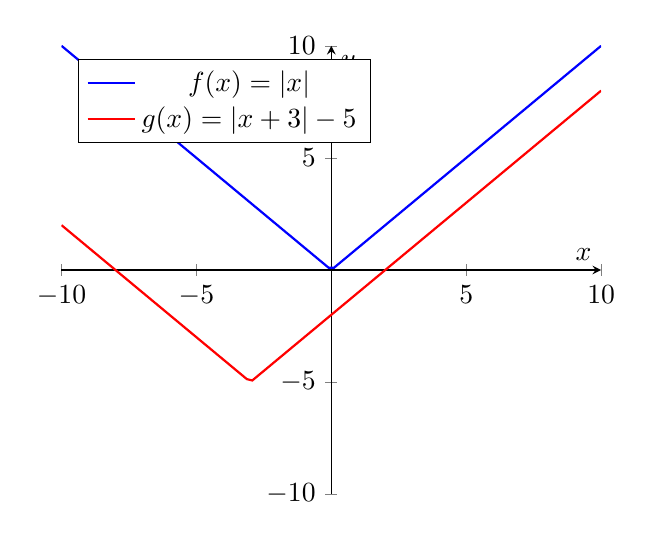
\begin{tikzpicture}
  \begin{axis}[
    axis lines=middle,
    xlabel={$x$},
    ylabel={$y$},
    ymin=-10, ymax=10,
    xmin=-10, xmax=10,
    domain=-10:10,
    samples=100,
    legend pos=north west
    ]
    \addplot [blue, thick] {abs(x)};
    \addplot [red, thick] {abs(x+3) - 5};
    \legend{$f(x) = |x|$, $g(x) = |x+3| - 5$}
  \end{axis}
\end{tikzpicture}
} {}{NOTAGS}

\ex
{\code{FxTRx25x02x05x013}}{40}
{
Consider $g(x) = 2 + \dfrac{1}{3x}$.
On one axis graph the basic function it is transformed from.
Then on another axis, graph $g(x)$ using graph transformations.

}
{

 

The basic function that $g(x) = 2 + \frac{1}{3x}$ is transformed from is $f(x) = \frac{1}{x}$.

Graph of the basic function $f(x) = \frac{1}{x}$:

\[
\begin{array}{c|c}
x & f(x) \\
\hline
-2 & -\frac{1}{2} \\
-1 & -1 \\
-0.5 & -2 \\
0.5 & 2 \\
1 & 1 \\
2 & \frac{1}{2} \\
\end{array}
\]

\begin{tikzpicture}
\begin{axis}[
    axis lines = center,
    xlabel = $x$,
    ylabel = $f(x)$,
    ymin = -2, ymax = 2,
    xmin = -2, xmax = 2,
]
\addplot [
    domain=-2:-0.1, 
    samples=100, 
    color=blue,
]
{1/x};
\addplot [
    domain=0.1:2, 
    samples=100, 
    color=blue,
]
{1/x};
\end{axis}
\end{tikzpicture}

Graph of $g(x) = 2 + \frac{1}{3x}$ using transformations:

1. Horizontal compression by a factor of 3: $f\left(\frac{x}{3}\right) = \frac{1}{3x}$
2. Vertical shift up by 2 units.

Graph after transformations:

\[
\begin{array}{c|c}
x & g(x) \\
\hline
-2 & 2 - \frac{1}{6} \\
-1 & 2 - \frac{1}{3} \\
-0.5 & 2 - \frac{2}{3} \\
0.5 & 2 + \frac{2}{3} \\
1 & 2 + \frac{1}{3} \\
2 & 2 + \frac{1}{6} \\
\end{array}
\]

\begin{tikzpicture}
\begin{axis}[
    axis lines = center,
    xlabel = $x$,
    ylabel = $g(x)$,
    ymin = 0, ymax = 4,
    xmin = -2, xmax = 2,
]
\addplot [
    domain=-2:-0.1, 
    samples=100, 
    color=red,
]
{2 + 1/(3*x)};
\addplot [
    domain=0.1:2, 
    samples=100, 
    color=red,
]
{2 + 1/(3*x)};
\end{axis}
\end{tikzpicture}
} {}{NOTAGS}


\ex
{\code{FxTRx25x02x05x014}}{40}
{
Consider $h(x) = 4 \cdot \sqrt{x - 2}$.
On one axis graph the basic function it is transformed from.
Then on another axis, graph $h(x)$ using graph transformations.

}
{

 

The basic function is $f(x) = \sqrt{x}$.

The graph of $h(x) = 4 \cdot \sqrt{x - 2}$ is obtained by applying the following transformations to $f(x)$:

1. Horizontal shift to the right by 2 units: $f(x - 2) = \sqrt{x - 2}$.
2. Vertical stretch by a factor of 4: $4 \cdot \sqrt{x - 2}$.

% Basic function
\[
\begin{array}{|c|c|}
\hline
x & f(x) = \sqrt{x} \\
\hline
0 & 0 \\
1 & 1 \\
4 & 2 \\
9 & 3 \\
\hline
\end{array}
\]

% Transformed function
\[
\begin{array}{|c|c|}
\hline
x & h(x) = 4 \cdot \sqrt{x - 2} \\
\hline
2 & 0 \\
3 & 4 \\
6 & 8 \\
11 & 12 \\
\hline
\end{array}
\]
} {}{NOTAGS}

\ex
{\code{FxTRx25x02x05x015}}{40}
{
Consider $h(x) =  2^{x - 2} - 2$.
On one axis graph the basic function it is transformed from.
Then on another axis, graph $h(x)$ using graph transformations.

}
{

 

The basic function from which $h(x) = 2^{x-2} - 2$ is transformed is $f(x) = 2^x$. 

To graph $h(x)$ using graph transformations:

1. **Horizontal Shift**: The term $x-2$ indicates a horizontal shift to the right by 2 units. Thus, the function becomes $g(x) = 2^{x-2}$.

2. **Vertical Shift**: The term $-2$ outside indicates a vertical shift downward by 2 units. Thus, the function is $h(x) = 2^{x-2} - 2$.

The transformations can be summarized as:

1. Start with the basic graph of $f(x) = 2^x$.
2. Shift the graph right by 2 units to get $g(x) = 2^{x-2}$.
3. Shift the graph down by 2 units to obtain $h(x) = 2^{x-2} - 2$.

Graph sketches are done as follows:

For $f(x) = 2^x$:

- The graph passes through the point $(0, 1)$.
- It is an exponential growth curve with a horizontal asymptote at $y = 0$.

For $h(x) = 2^{x-2} - 2$:

- The graph passes through the point $(2, 0)$.
- It is an exponential curve with a horizontal asymptote at $y = -2$.
} {}{NOTAGS}

\ex
{\code{FxTRx25x02x05x016}}{40}
{
Consider $f(x) = -3x^2 - 4$.
On one axis graph the basic function it is transformed from.
Then on another axis, graph $f(x)$ using graph transformations.

}
{

 

The basic function that $f(x) = -3x^2 - 4$ is transformed from is $g(x) = x^2$.

On the first axis, the graph of $g(x) = x^2$ is a parabola that opens upwards with its vertex at the origin $(0,0)$.

\[ 
\begin{array}{c|c}
x & g(x) = x^2 \\
\hline
-2 & 4 \\
-1 & 1 \\
0 & 0 \\
1 & 1 \\
2 & 4 \\
\end{array} 
\]

On the second axis, apply the transformations to graph $f(x) = -3x^2 - 4$. The transformations applied to $g(x) = x^2$ include:

1. Vertical stretch by a factor of 3, giving $3x^2$.
2. Reflection over the x-axis, giving $-3x^2$.
3. Vertical shift downward by 4 units, giving $-3x^2 - 4$.

The graph of $f(x) = -3x^2 - 4$ is a parabola that opens downwards with its vertex at $(0, -4)$.

\[ 
\begin{array}{c|c}
x & f(x) = -3x^2 - 4 \\
\hline
-2 & -16 \\
-1 & -7 \\
0 & -4 \\
1 & -7 \\
2 & -16 \\
\end{array} 
\]

Graphically, these transformations would be performed on two separate axes as described above.
} {}{NOTAGS}

\ex
{\code{FxTRx25x02x05x017}}{40}
{
Consider $f(x) = 4^{-x}$.
On one axis graph the basic function it is transformed from.
Then on another axis, graph $f(x)$ using graph transformations.

}
{

 

The basic function from which \( f(x) = 4^{-x} \) is transformed is \( g(x) = 4^x \).

First, graph the basic function \( g(x) = 4^x \):

\[
\begin{array}{c|c}
x & g(x) = 4^x \\
\hline
-2 & \frac{1}{16} \\
-1 & \frac{1}{4} \\
0 & 1 \\
1 & 4 \\
2 & 16 \\
\end{array}
\]

\begin{tikzpicture}
\begin{axis}[
    axis lines = middle,
    xlabel = $x$,
    ylabel = $g(x)$,
    ymin = 0, ymax = 20,
    xmin = -2, xmax = 2,
    samples = 100,
    domain = -2:2,
    restrict y to domain=0:20
]
\addplot[blue, thick] {4^x};
\end{axis}
\end{tikzpicture}

Now, graph \( f(x) = 4^{-x} \):

\[
f(x) = \frac{1}{4^x} \quad \text{(reflection over the \( y \)-axis)}
\]

\junk{
\begin{array}{c|c}
x & f(x) = 4^{-x} \\
\hline
-2 & 16 \\
-1 & 4 \\
0 & 1 \\
1 & \frac{1}{4} \\
2 & \frac{1}{16} \\
\end{array}

\begin{tikzpicture}
\begin{axis}[
    axis lines = middle,
    xlabel = $x$,
    ylabel = $f(x)$,
    ymin = 0, ymax = 20,
    xmin = -2, xmax = 2,
    samples = 100,
    domain = -2:2,
    restrict y to domain=0:20
]
\addplot[red, thick] {4^(-x)};
\end{axis}
\end{tikzpicture}
}
} {}{NOTAGS}


\ex
{\code{TESTxFxTRx25x02x14x001}}{10}
{How does $f(x - 4) - 8$ transform the graph of $f(x)$? 

}
{

 

The graph of \( f(x) \) is transformed by shifting it 4 units to the right and 8 units down.
} {}{NOTAGS}


\ex
{\code{TESTxFxTRx25x02x14x002}}{10}
{
Write a formula for the
function obtained when the
graph of $f(x) = x^4$ is
shifted down 3 units and to the
left 5 units. 

}
{

 

$f(x) = x^4$

Shifted down 3 units: $f(x) - 3 = x^4 - 3$

Shifted to the left 5 units: $f(x+5) = (x+5)^4$

Combined transformation: $f(x+5) - 3 = (x+5)^4 - 3$
} {}{NOTAGS}


\ex
{\code{FxTRx25x09x15x002}}{10}
{
Write a formula for the
function obtained when the
graph of $f(x) = \sqrt{x}$ is
shifted up 2 units and to the
right 3 units. 

}
{

SOLUTION:

$g(x) = 2+ \sqrt{x - 3}$ since adding outside is a vertical shift (up for positive), while adding inside is a horizontal shift (right for negative).

} {}{type: TEST}



\ex
{\code{TESTxFxTRx25x02x14x003}}{15}
{Suppose $g(x)$ is function defined everywhere.
Suppose $h(x) = 4 \ g(x)$.

\begin{multicols}{2}
\begin{enumerate}

\item
How is the graph of $h$ transformed from the graph of $g(x)$?

\item
If  $g(-2) = 3$, then what is $h(-2)$?

\end{enumerate}
\end{multicols}

}
{

 

The graph of $h(x) = 4 \, g(x)$ is a vertical stretch of the graph of $g(x)$ by a factor of 4.

If $g(-2) = 3$, then $h(-2) = 4 \cdot g(-2) = 4 \cdot 3 = 12$.
} {}{NOTAGS}



\ex
{\code{TESTxFxTRx25x02x14x004}}{40}
{
Let $h(x) =  (x - 3)^2 + 1$.

\begin{multicols}{2}
\begin{enumerate}

\item
On one axis, graph the basic function that $h(x)$ is transformed from (right below here).

\item
Then on another axis, graph $h(x)$ using graph transformations (right below here).

\end{enumerate}
\end{multicols}



}
{

 

The basic function that $h(x)$ is transformed from is $f(x) = x^2$. 
To graph $h(x)$ using transformations:

1. Start with $f(x) = x^2$.
2. Apply a horizontal shift to the right by 3 units: $f(x - 3) = (x - 3)^2$.
3. Apply a vertical shift up by 1 unit: $h(x) = (x - 3)^2 + 1$.

The graphs are as follows:

\begin{center}
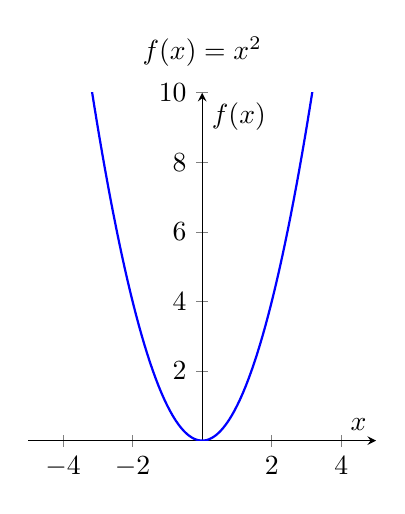
\begin{tikzpicture}
    % Graph of f(x) = x^2
    \begin{axis}[
        axis lines = middle,
        xlabel = $x$,
        ylabel = {$f(x)$},
        ymin=0, ymax=10,
        xmin=-5, xmax=5,
        domain=-4:4,
        samples=100,
        width=6cm,
        height=6cm,
        title={$f(x) = x^2$}
    ]
    \addplot [domain=-4:4, thick, blue] {x^2};
    \end{axis}
\end{tikzpicture}
\quad
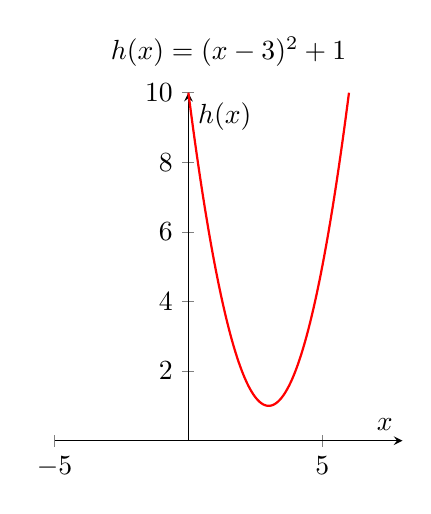
\begin{tikzpicture}
    % Graph of h(x) = (x - 3)^2 + 1
    \begin{axis}[
        axis lines = middle,
        xlabel = $x$,
        ylabel = {$h(x)$},
        ymin=0, ymax=10,
        xmin=-5, xmax=8,
        domain=0:6,
        samples=100,
        width=6cm,
        height=6cm,
        title={$h(x) = (x-3)^2 + 1$}
    ]
    \addplot [domain=0:6, thick, red] {(x-3)^2 + 1};
    \end{axis}
\end{tikzpicture}
\end{center}
} {}{NOTAGS}



\ex
{\code{FxTRx25x02x14x004}}{40}
{
In your graphs, clearly label the axes so that the transformation from $f$ to $h$ is clear.

\begin{multicols}{2}
\begin{enumerate}

\item Right below here graph the function $f(x) = x^2$

\item Right below here graph the function $h(x) = (x - 1)^2 + 2$ 

\end{enumerate}
\end{multicols}



}
{

 

\[
\begin{array}{c}
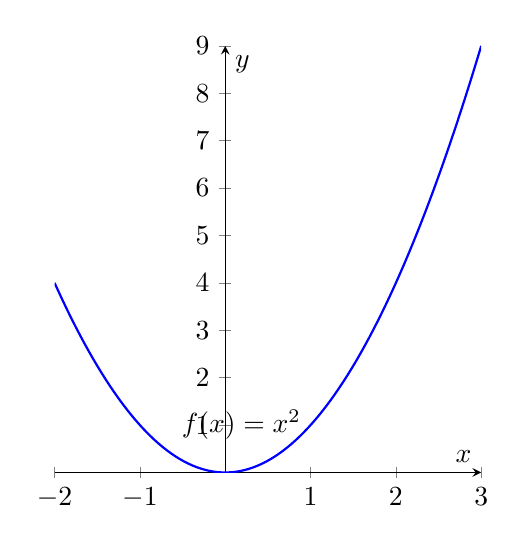
\begin{tikzpicture}
    \begin{axis}[
        axis lines = middle, 
        xlabel = {$x$}, 
        ylabel = {$y$}, 
        domain=-2:3, 
        samples=100,
        width=7cm,
        height=7cm,
        xtick distance=1,
        ytick distance=1
        ]
        \addplot [blue, thick] {x^2};
        \node at (axis cs:1,1) [anchor=east] {$f(x) = x^2$};
    \end{axis}
\end{tikzpicture}
\end{array}
\quad
\begin{array}{c}
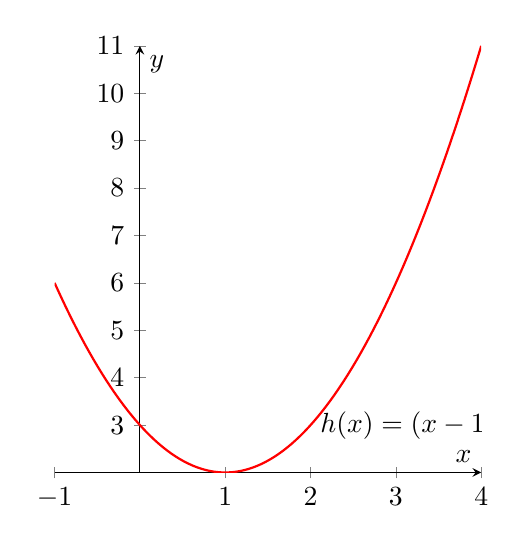
\begin{tikzpicture}
    \begin{axis}[
        axis lines = middle, 
        xlabel = {$x$}, 
        ylabel = {$y$}, 
        domain=-1:4, 
        samples=100,
        width=7cm,
        height=7cm,
        xtick distance=1,
        ytick distance=1
        ]
        \addplot [red, thick] {(x - 1)^2 + 2};
        \node at (axis cs:2,3) [anchor=west] {$h(x) = (x-1)^2 + 2$};
    \end{axis}
\end{tikzpicture}
\end{array}
\]
} {}{type: TEST}





\ex
{\code{GPTx26x02x20x011}}{40}
{
Let $h(x)=(x+2)^2-4$.

\begin{multicols}{2}
\begin{enumerate}
\item Graph the basic function from which $h(x)$ is transformed.
\item Graph $h(x)$ using transformations.
\end{enumerate}
\end{multicols}
}
{

 

The basic function from which \( h(x) \) is transformed is \( f(x) = x^2 \).

To graph \( h(x) = (x+2)^2 - 4 \) using transformations, perform the following steps:

1. **Horizontal Shift:** \( (x+2)^2 \) represents a shift left by 2 units of the basic function \( f(x) = x^2 \).

2. **Vertical Shift:** The term \(-4\) indicates a shift down by 4 units.

Thus, the graph of \( h(x) \) is the graph of \( f(x) = x^2 \) shifted 2 units to the left and 4 units down.
} {}{type: TEST}



\ex
{\code{GPTx26x02x20x013}}{15}
{
Write a formula for the function obtained when the graph of $f(x)=\sqrt{x}$ is shifted down 1 unit and left 4 units.
}
{

 

Shift left 4 $\rightarrow$ replace $x$ with $x+4$.
Shift down 1 $\rightarrow$ subtract 1.

New function: $y=\sqrt{x+4}-1$.
} {}{type: TEST}

\ex
{\code{GPTx26x02x20x014}}{20}
{
Consider the function $f(x)=-(x-2)^2$.

\begin{enumerate}
\item Where is it increasing?
\item Where is it decreasing?
\item Find the absolute extrema (if it does not have a max or min, state this).
\item Find the local extrema (if it does not have a max or min, state this).
\end{enumerate}
}
{

 

This is $y = x^2$ shifted to the right 2, then reflected across the x-axis.
So it has an absolute maximum at $(2, 0)$, increasing up to that point, then decreasing.  Thus we have th following.

a) Increasing on interval $(-\infty,2)$  

b) Decreasing on interval  $(2, +\infty)$

c) Absolute max at $(2, 0)$.  No absolute min, since it decreases without bound.

d) Local max also at $(2, 0)$. No local min.


} {}{type: TEST}





\ex
{\code{GROUPxFxTRx25x02x10x001}}{90}
{
Graph $f(x) = \sin (x)$ in Desmos. Use Desmos (and your brain!) to do the following:

\begin{enumerate}

\item Add an additional plot of $g(x) = 5 \sin (x)$. 
Descibe how this transforms $f(x)$ and make a rough sketch of $f$ and $g$ on the same axes.

\item Add an additional plot of $h(x) =  \frac{1}{5} \sin (x)$. 
Descibe how this transforms $f(x)$ and make a rough sketch of $f$ and $h$ on the same axes.


\item Add an additional plot of $A(x) = \sin (5x)$. 
Descibe how this transforms $f(x)$ and make a rough sketch of $f$ and $A$ on the same axes.

\item Add an additional plot of $B(x) =  \sin ( \frac{1}{5}x)$. 
Descibe how this transforms $f(x)$ and make a rough sketch of $f$ and $B$ on the same axes.



\end{enumerate}

}
{

 

\begin{enumerate}

\item The function $g(x) = 5 \sin(x)$ vertically stretches the graph of $f(x) = \sin(x)$ by a factor of 5. This means the amplitude increases from 1 to 5. 

\begin{center}
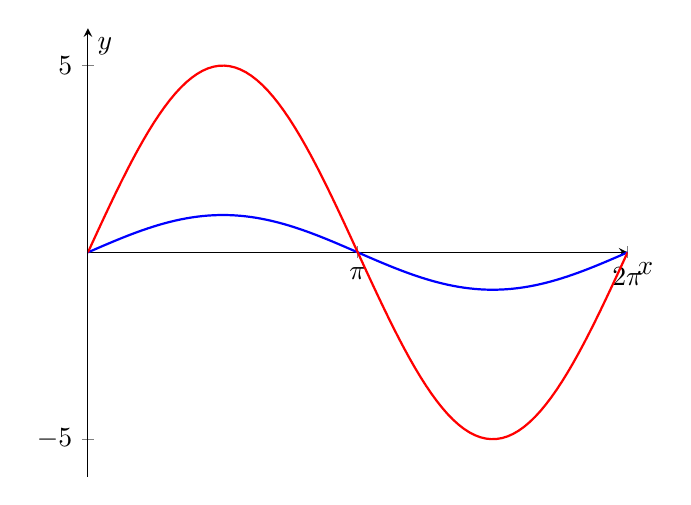
\begin{tikzpicture}
\begin{axis}[domain=0:2*pi, samples=100, axis lines=middle, xlabel={$x$}, ylabel={$y$}, xtick={0, pi, 2*pi}, xticklabels={$0$, $\pi$, $2\pi$}, ytick={-5, 0, 5}, ymin=-6, ymax=6, xlabel style={below right}]
\addplot[blue, thick] {sin(deg(x))};
\addplot[red, thick] {5*sin(deg(x))};
\end{axis}
\end{tikzpicture}
\end{center}

\item The function $h(x) = \frac{1}{5} \sin(x)$ vertically compresses the graph of $f(x) = \sin(x)$ by a factor of $\frac{1}{5}$. This means the amplitude decreases from 1 to $\frac{1}{5}$. 

\begin{center}
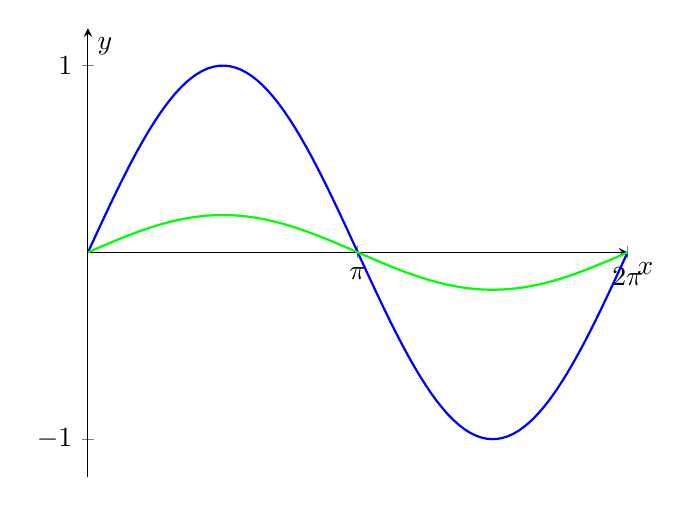
\begin{tikzpicture}
\begin{axis}[domain=0:2*pi, samples=100, axis lines=middle, xlabel={$x$}, ylabel={$y$}, xtick={0, pi, 2*pi}, xticklabels={$0$, $\pi$, $2\pi$}, ytick={-1, 0, 1}, ymin=-1.2, ymax=1.2, xlabel style={below right}]
\addplot[blue, thick] {sin(deg(x))};
\addplot[green, thick] {0.2*sin(deg(x))};
\end{axis}
\end{tikzpicture}
\end{center}

\item The function $A(x) = \sin(5x)$ compresses the graph of $f(x) = \sin(x)$ horizontally by a factor of 5, increasing the frequency of the wave. The period changes from $2\pi$ to $\frac{2\pi}{5}$.

\begin{center}
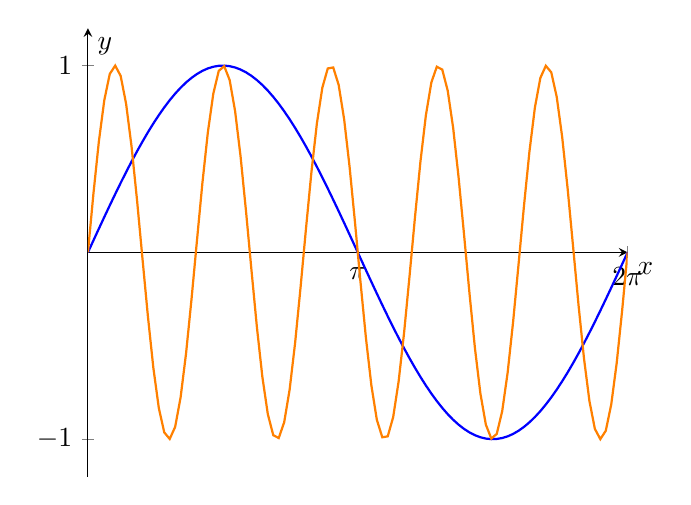
\begin{tikzpicture}
\begin{axis}[domain=0:2*pi, samples=100, axis lines=middle, xlabel={$x$}, ylabel={$y$}, xtick={0, pi, 2*pi}, xticklabels={$0$, $\pi$, $2\pi$}, ytick={-1, 0, 1}, ymin=-1.2, ymax=1.2, xlabel style={below right}]
\addplot[blue, thick] {sin(deg(x))};
\addplot[orange, thick] {sin(deg(5*x))};
\end{axis}
\end{tikzpicture}
\end{center}

\item The function $B(x) = \sin\left(\frac{1}{5}x\right)$ stretches the graph of $f(x) = \sin(x)$ horizontally by a factor of 5, decreasing the frequency of the wave. The period changes from $2\pi$ to $10\pi$.

\begin{center}
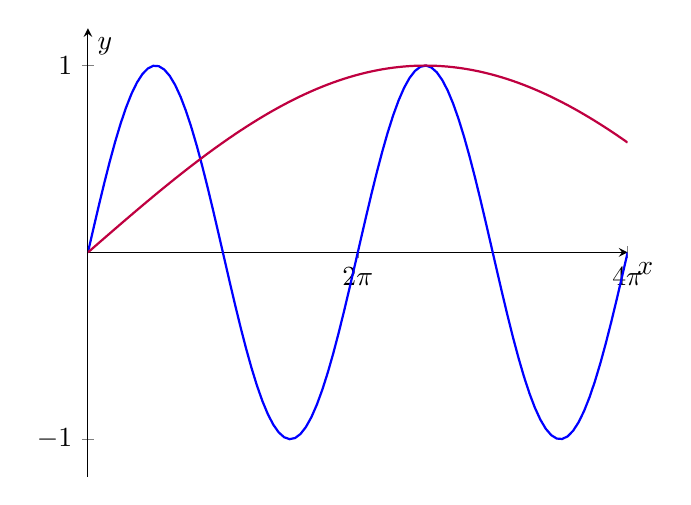
\begin{tikzpicture}
\begin{axis}[domain=0:4*pi, samples=100, axis lines=middle, xlabel={$x$}, ylabel={$y$}, xtick={0, 2*pi, 4*pi}, xticklabels={$0$, $2\pi$, $4\pi$}, ytick={-1, 0, 1}, ymin=-1.2, ymax=1.2, xlabel style={below right}]
\addplot[blue, thick] {sin(deg(x))};
\addplot[purple, thick] {sin(deg(x/5))};
\end{axis}
\end{tikzpicture}
\end{center}

\end{enumerate}
} {}{NOTAGS}




\subsection{Function Applications \topic{APP}} 

\ex
{\code{FxAPPx25x01x23x001}}{10}
{
 Let $D(t)$ be your distance (in miles) from BCC $t$ hours after noon on
 January 1, 2025. Explain the meaning
of each statement:
\begin{enumerate}
\item $D(3) = 10$

\item $D(1) = 0$

\item $D(0) = 2$ 
\end{enumerate}
}
{

 

$D(3) = 10$: Three hours after noon on January 1, 2025, you are 10 miles away from BCC.

$D(1) = 0$: One hour after noon on January 1, 2025, you are at BCC.

$D(0) = 2$: At noon on January 1, 2025, you are 2 miles away from BCC.
} {}{NOTAGS}
 


\subsection{Functions \topic{MIXED}} 
 
\ex
{\code{FxMIXEDx25x01x21x008}}{50}
{
Consider the function \(f(x) = 2 + \sqrt{x}\).
Do the following.
\begin{multicols}{2}
\begin{enumerate}

\item Graph it.
\item Find domain and range.
\item Is it one-to-one?
\item Does it have an inverse?
\item If it has an inverse, find the domain and range of that inverse.

\end{enumerate}
\end{multicols}
}
{

 

\junk{
\[
\begin{aligned}
&\text{The graph of \(f(x) = 2 + \sqrt{x}\) is a transformation of the basic square root function.} \\
&\text{Domain: } x \geq 0. \\
&\text{Range: } y \geq 2. \\
&\text{The function is one-to-one because it is strictly increasing on its domain.} \\
&\text{Since it is one-to-one, it has an inverse.} \\
&\text{To find the inverse, solve } y = 2 + \sqrt{x} \text{ for } x. \\
&y - 2 = \sqrt{x} \\
&(y-2)^2 = x \\
&\text{So the inverse is } f^{-1}(x) = (x-2)^2. \\
&\text{Domain of the inverse: } x \geq 2. \\
&\text{Range of the inverse: } y \geq 0. \\
\end{aligned}
\]
}

} {}{NOTAGS}



\ex
{\code{FxMIXEDx25x01x21x009}}{50}
{
Consider the function \(g(x) = |x + 1|\)
Do the following.
\begin{multicols}{2}
\begin{enumerate}

\item Graph it.
\item Find domain and range.
\item Is it one-to-one?
\item Does it have an inverse?
\item If it has an inverse, find the domain and range of that inverse.

\end{enumerate}
\end{multicols}
}
{

 

\begin{enumerate}
    \item Graph it. 
    \begin{center}
    \begin{tikzpicture}
    \begin{axis}[
        axis lines = middle,
        xlabel = $x$,
        ylabel = $g(x)$,
        ymin = -1, ymax = 5,
        xmin = -5, xmax = 5,
        domain = -5:5,
        samples = 100,
        smooth,
        width=8cm,
        height=8cm
    ]
    \addplot[blue] {abs(x + 1)};
    \end{axis}
    \end{tikzpicture}
    \end{center}

    \item Find domain and range.

    \textbf{Domain:} $(-\infty, \infty)$

    \textbf{Range:} $[0, \infty)$

    \item Is it one-to-one?

    No, \(g(x)\) is not one-to-one because it does not pass the horizontal line test.

    \item Does it have an inverse?

    No, \(g(x)\) does not have an inverse because it is not a one-to-one function.

    \item If it has an inverse, find the domain and range of that inverse.

    This part is not applicable since \(g(x)\) does not have an inverse.
\end{enumerate}
} {}{NOTAGS}


\ex
{\code{FxMIXEDx25x01x22x005}}{20}
{
Find the domain and zeroes of \(g(x)=\frac{4x}{x^2 - 100}\).
}{

 

The domain of \(g(x)=\frac{4x}{x^2 - 100}\) is all real numbers except where the denominator is zero. Set the denominator equal to zero and solve:

\[ 
x^2 - 100 = 0 
\]

\[ 
x^2 = 100 
\]

\[ 
x = \pm 10 
\]

Thus, the domain is \(x \in \mathbb{R} \setminus \{-10, 10\}\).

To find the zeroes of \(g(x)\), set the numerator equal to zero:

\[ 
4x = 0 
\]

\[ 
x = 0 
\]

The zero of \(g(x)\) is \(x = 0\).

Therefore, the domain is \(x \in \mathbb{R} \setminus \{-10, 10\}\) and the zero is \(x = 0\).
}{}{NOTAGS}


\ex
{\code{FxMIXEDx25x01x22x008}}{50}
{
For \(f(x)=3 + 2^{x+1}\), give the horizontal asymptote, domain, range, end behavior, and sketch its graph.
}{

 

The horizontal asymptote of \(f(x) = 3 + 2^{x+1}\) is \(y = 3\).

The domain of \(f(x)\) is \((-\infty, \infty)\).

The range of \(f(x)\) is \((3, \infty)\).

As \(x \to -\infty\), \(f(x) \to 3\).

As \(x \to \infty\), \(f(x) \to \infty\).

[Sketch of the graph can be indicated by noting the exponential nature of \(2^{x+1}\), starting from above \(y = 3\) and increasing without bound.]
}{}{NOTAGS}


\ex
{\code{FxMIXEDx25x01x22x011}}{50}
{
Consider \(f(x)=\log_3(x-2)\). Find its domain, range, and vertical asymptote. Sketch the graph.
}{

 

The domain of \( f(x) = \log_3(x-2) \) is found by setting the argument of the logarithm greater than zero:

\[ x - 2 > 0 \]

\[ x > 2 \]

So, the domain is \( (2, \infty) \).

The range of any logarithmic function is all real numbers, hence the range of \( f(x) \) is:

\[ (-\infty, \infty) \]

The vertical asymptote occurs where the argument of the logarithm equals zero:

\[ x - 2 = 0 \]

\[ x = 2 \]

Therefore, the vertical asymptote is \( x = 2 \).

To sketch the graph of \( f(x) = \log_3(x-2) \):

- Plot the vertical asymptote at \( x = 2 \).
- Since the function is a logarithm with base greater than 1, it will increase logarithmically as \( x \) increases.
- The graph passes through the point where \( x = 3 \), i.e., \( f(3) = \log_3(3-2) = \log_3(1) = 0 \).

\[
\begin{array}{l}
\text{Domain: } (2, \infty) \\
\text{Range: } (-\infty, \infty) \\
\text{Vertical Asymptote: } x = 2 \\
\end{array}
\]

Sketch of the graph:

- The curve approaches \( x = 2 \) but never touches it, rising from negative infinity.
- Passes through \( (3, 0) \).
- Moves upwards to the right.
}{}{NOTAGS}



\ex
{\code{TESTxxxFxMIXEDx25x04x28x001}}{40}
{For each function, find its domain and range.
\begin{multicols}{2}
\begin{enumerate}
\item $h(x) = 3 + \sqrt{7x - 1}$
\item  \(f(x)= -6 + \ln (5x + 2)\)
\end{enumerate}
\end{multicols} 

}{

SOLUTION:

\begin{enumerate}
\item For the domain, solve $7x - 1 \ge 0$: $x \ge \frac{1}{7}$, so the domain is 
$[\frac{1}{7}, +\infty)$.

For the range, we note that $h(x)$ is the square root function $\sqrt{x}$ (with range $[0, +\infty)$ )
with some horizontal modification (not relevant to the range), but shifted up 3, so the
the range is  $[3, +\infty)$

\vspace{4mm}

\item  For the domain, solve $5x + 2 > 0$: $x > \frac{-2}{5}$, so the domain is
$(\frac{-2}{5}, +\infty)$.

The range is $(-\infty, +\infty)$, since the starting function $\ln (x)$ has range 
$(-\infty, +\infty)$, and moving it horizontally and vertically does not change this.

\end{enumerate}

}{}{NOTAGS}



\subsection{Functions with Domain/coDomain} 


\ex
{\code{Fx25x10x12x001}}{30}
{
Let $A = \{0, 2, 4, 6, 8 \}$ and $B = \{0, 1, 2, 3, 4, 5, 6 \}$.

Let the function $f:A \rightarrow B$ be defined by 
$f(n) = n/2$.

\begin{enumerate}

\item What are the domain and codomain of $f$?

\item   Is $f$ injective?

\item What is the range of $f$?

\item
Why is $f$ not surjective? Is there any surjective function from $A$ to $B$?

\end{enumerate}

}{

 

Domain of $f$ is $A = \{0, 2, 4, 6, 8\}$.

Codomain of $f$ is $B = \{0, 1, 2, 3, 4, 5, 6\}$.

$f$ is injective because for each $n_1, n_2 \in A$, if $f(n_1) = f(n_2)$, then $n_1/2 = n_2/2$ implies $n_1 = n_2$.

Range of $f$ is $\{0, 1, 2, 3, 4\}$.

$f$ is not surjective because there are elements in $B$ (e.g., $5, 6$) that are not covered by $f$. There is no surjective function from $A$ to $B$ because $A$ has fewer elements than $B$.
}{}{type: HW , topics: FUNCT}




\ex
{\code{Fx25x10x12x002}}{30}
{
Let $A = \{0, 2, 4, 6, 8 \}$ and $B = \{3, 4, 5, 6 \}$.

\begin{enumerate}

\item Let the function $h:A \rightarrow B$ be defined by:
$$h(0) = 6, \  \ h(2) = 5,  \  \  h(4) = 4,  \  \  h(6) = 3,  \  \  h(8) = 6.$$  
Is $h$ surjective?

\item
Why is $h$ not injective? Is there any injective function from $A$ to $B$?

\end{enumerate}

}{

 

\begin{enumerate}
    \item To determine if $h$ is surjective, we check if every element in $B$ is mapped by some element in $A$. The elements of $B$ are $\{3, 4, 5, 6\}$. From the given definition of $h$:

    \begin{align*}
    h(0) &= 6, \\
    h(2) &= 5, \\
    h(4) &= 4, \\
    h(6) &= 3, \\
    h(8) &= 6. \\
    \end{align*}

    All elements of $B$ are covered. Thus, $h$ is surjective.

    \item The function $h$ is not injective because $h(0) = 6$ and $h(8) = 6$, meaning two different elements in $A$ are mapped to the same element in $B$. 

    To find an injective function from $A$ to $B$, consider a function that maps every element of $A$ to a unique element in $B$. However, since $|A| = 5$ and $|B| = 4$, there cannot be an injective function from $A$ to $B$, because an injective function requires that $|A| \leq |B|$.
\end{enumerate}
}{}{type: HW , topics: FUNCT}


\ex
{\code{Fx25x10x12x003}}{60}
{
Let $X = \{ u \in \mathcal{Z} \ | \ 1 \le u \le 100 \}$ and 
$Y = \{u \in \mathcal{Z} \ | \ 10 \le u \le 109  \}$.
 Let the function $h:X \rightarrow Y$ be defined by $h(n) = n + 9$.
 Prove that $h$ is bijective. Why does $h$ have an inverse?  What is $h^{-1}(109)$?

}{

SOLUTION:

$h^{-1}(109) = 100$ since $h(100) = 109$.

\vspace{2mm}

$h$ is injective because:
$h(x) = h(y) \rightarrow x+9 = y +9 \rightarrow x = y$

$h$ is surjective because:
For any $y$ where $10 \le y \le 109$, we can find an $x$ so that $h(x) = y$,
by letting $x = y - 9$. Note that $1 \le x \le 100$, so
$x$ is in the domain of $h$.  Furthermore, 
$h(x) = y - 9 + 9 = y$.

\vspace{2mm}

Since $h$ is injective and surjective, by definition, $h$ is bijective.
Since $h$ is bijective, a theorem tells us that $h$ has an inverse.

}{}{type: HW , topics: FUNCT}



\ex
{\code{Fx25x11x05x002}}{50}
{
Let $X = \{ u \in \mathcal{Z} \ | \ 1 \le u \le 100 \}$ and 
$Y = \{u \in \mathcal{Z} \ | \ -100 \le u \le -1  \}$.
 Let the function $h:X \rightarrow Y$ be defined by $h(n) = -101 + n$.
 Prove that $h$ is bijective. Why does $h$ have an inverse?  What is $h^{-1}(-50)$?

}{

 

To prove that the function \( h: X \rightarrow Y \) defined by \( h(n) = -101 + n \) is bijective, we need to show that it is both injective and surjective.

**Injectivity:**

Suppose \( h(n_1) = h(n_2) \). Then:

\[
-101 + n_1 = -101 + n_2
\]

Adding 101 to both sides, we get:

\[
n_1 = n_2
\]

Therefore, \( h \) is injective.

**Surjectivity:**

Let \( v \in Y \) such that \( -100 \le v \le -1 \). We need to find an \( n \in X \) such that \( h(n) = v \).

Set:

\[
-101 + n = v
\]

Solving for \( n \), we get:

\[
n = v + 101
\]

Since \( -100 \le v \le -1 \), we have:

\[
1 \le v + 101 \le 100
\]

Thus, \( n = v + 101 \in X \). Therefore, \( h \) is surjective.

Since \( h \) is both injective and surjective, \( h \) is bijective.

**Inverse Function:**

Because \( h \) is bijective, it has an inverse function \( h^{-1}: Y \rightarrow X \).

**Find \( h^{-1}(-50) \):**

Set \( h(n) = -50 \):

\[
-101 + n = -50
\]

Solving for \( n \), we add 101 to both sides:

\[
n = -50 + 101 = 51
\]

Thus, \( h^{-1}(-50) = 51 \).
}{}{type: TEST , topics: FUNCT}





\ex
{\code{Fx25x10x12x004}}{40}
{
Let $X = \{ u \in \mathcal{Z} \ | \ 1 \le u \le 10 \}$.
 Let the function $h:X \rightarrow X$ be defined by 
 $h(n) = \begin{cases}
 n + 1 \hbox{ if $n$ is odd} \\
 n/2 \hbox{ if $n$ is even}
 \end{cases}$
 
 \begin{enumerate}
 
 \item
Describe the range of $h$.  Is $h$ onto? 

\item
Use the same definition for $h$, but now let $X = \{ u \in Z \ | \ 1 \le u \le 100 \}$.
Describe the new range.

\end{enumerate}
 
}{

 

The range of $h$ when $X = \{ u \in \mathcal{Z} \ | \ 1 \le u \le 10 \}$ is $\{2, 3, 4, 5, 6\}$. To determine if $h$ is onto, observe that not every element in $X$ is an image under $h$. Hence, $h$ is not onto.

Now, considering $X = \{ u \in \mathcal{Z} \ | \ 1 \le u \le 100 \}$, the range of $h$ covers all numbers of the form $2, 3, 4, \ldots, 50$, and potentially more. Hence, the range is larger but still does not cover $X$ fully; $h$ is not onto.
}{}{type: HW , topics: FUNCT}



\ex 
{\code{Fx25x10x27x004}}{40}
{
Let $X = \{ u \in \mathcal{Z} \ | \ 1 \le u \le 100 \}$.
 Let the function $f:X \rightarrow X$ be defined by 
 $$f(n) = \begin{cases}
 n  \hbox{ if $n$ is odd} \\
 n-1 \hbox{ if $n$ is even}
 \end{cases}$$
 
 \begin{enumerate}
 
 \item Is $f$ injective?
 
 \item
Describe the range of $f$.  Is $f$ onto? 

\item Does $f$ have an inverse function?

\end{enumerate}
 
}{

 

\begin{enumerate}
\item The function $f$ is injective. For $n$ odd, $f(n) = n$, and for $n$ even, $f(n) = n-1$. Distinct $n_1$ and $n_2$ in $X$ produce distinct results, because either they are both odd, or at least one is even leading to unique outputs. Thus, $f$ is injective.

\item The range of $f$ is all odd numbers from 1 to 99, inclusive, i.e., $\{1, 3, 5, \ldots, 99\}$. The function is not onto because not every element in $X$ is an odd number; hence there are elements in $X$ that are not in the range of $f$.

\item The function $f$ does not have an inverse function because it is not onto. An inverse would require $f$ to map every element in the range back to a unique element in the domain, but since $f$ is not onto, this requirement is not satisfied.
\end{enumerate}
}{}{type: TEST , topics: FUNCT}




\ex 
{\code{Fx25x12x11x001}}{40}
{
Let $X = \{ u \in \mathcal{Z} \ | \ 1 \le u \le 10 \}$ and let
$Y = \{v \in \mathcal{Z} \ | \ 0 \le v \le 20 \}$.

Define $f: X \rightarrow Y$ by $f(x) = 20 - 2x$.

 
 \begin{enumerate}
 
 \item Is $f$ injective?
 
 \item
Describe the range of $f$.  Is $f$ onto? 

\item Is $f$ bijective?

\item Does $f$ have an inverse function?

\end{enumerate}
 
}{

 

\begin{enumerate}

\item 
Yes. Since $f(x) = f(y) \Rightarrow 20 -2x = 20 -2y \Rightarrow -2x = - 2y
\Rightarrow x = y$

\item
Range $= \{ 0, 2, \ldots, 18 \}$, i.e the evens between $0$ and $18$ (inclusive),
since $f(1) = 18, f(2) = 16, \ldots, f(10) = 0$.

It is not onto, since many elements of the codmain $Y$ are not in the range
(point out any of these: $1, 3, \ldots, 17, 19, 20$).

\item Not bijective. Since not onto.

\item Not have an inverse, since not bijective.

\end{enumerate}

}{}{type: TEST , topics: FUNCT}




\ex
{\code{Fx25x10x12x005}}{50}
{
For each function $Z \times Z \rightarrow Z$, determine if it is
i) onto?, ii) one-to-one?, iii) bijective?
 
 \begin{multicols}{2}
 \begin{enumerate}
 
 \item
$f(a, b) = a - b$

\item
$g(x, y) = x^2 + x^4$


\end{enumerate}
\end{multicols}
 
}{

 

i) $f(a, b) = a - b$

- **Onto**: Yes, for any integer $c$, choose $a = c + b$. Then $f(a, b) = c$.
- **One-to-one**: No, $f(a, b) = 0$ for $a = b$ and $f(a', b') = 0$ for $a' = b'$, giving the same output for different inputs.
- **Bijective**: No, since it is not one-to-one.

ii) $g(x, y) = x^2 + x^4$

- **Onto**: No, $g(x, y)$ always gives non-negative results, cannot produce negative integers.
- **One-to-one**: No, $g(x, 0) = x^2$ and $g(x, 0) = x^2$ for any $y$.
- **Bijective**: No, since it is neither onto nor one-to-one.
}{}{type: HW , topics: FUNCT}




\ex
{\code{Fx25x11x05x006}}{50}
{
For each function $Z \times Z \rightarrow Z$, determine if it is
i) onto?, ii) one-to-one?, iii) bijective?
 
 \begin{multicols}{2}
 \begin{enumerate}
 
 \item
$f(a, b) = a^6 + b^4 - 2$

\item
$g(x, y) = x^3 + y$


\end{enumerate}
\end{multicols}
 
}{

 

\textbf{1. Function $f(a, b) = a^6 + b^4 - 2$:}

i) \textit{Onto:} The codomain is $\mathbb{Z}$. Consider $z \in \mathbb{Z}$. We need $a^6 + b^4 - 2 = z$, which implies $a^6 + b^4 = z + 2$. 

For $z \to -\infty$, $a^6 + b^4 \geq -2$ shows there exist integers $a, b$ such that $a^6 + b^4 = n$ for any $n \geq -2$. However, no integer $a, b$ satisfy $a^6 + b^4 = -3$, indicating not all $z$ values are achievable. Therefore, $f$ is not onto.

ii) \textit{One-to-one:} Consider $f(a_1, b_1) = f(a_2, b_2)$. We have $a_1^6 + b_1^4 = a_2^6 + b_2^4$, but this does not guarantee $a_1 = a_2$ and $b_1 = b_2$. For example, $f(0, 1) = f(1, 0) = -1$ but $(0, 1) \neq (1, 0)$. Therefore, $f$ is not one-to-one.

iii) \textit{Bijective:} Since $f$ is neither onto nor one-to-one, it is not bijective. 

\textbf{2. Function $g(x, y) = x^3 + y$:}

i) \textit{Onto:} The codomain is $\mathbb{Z}$. For any $z \in \mathbb{Z}$, let $x = 0$ and $y = z$. Then $g(0, y) = 0 + y = z$. Thus, for every $z$, there exists $(x, y) = (0, z)$ such that $g(x, y) = z$. Therefore, $g$ is onto. 

ii) \textit{One-to-one:} Consider $g(x_1, y_1) = g(x_2, y_2)$. We have $x_1^3 + y_1 = x_2^3 + y_2$. It requires $x_1^3 = x_2^3$ and $y_1 = y_2$, which implies $x_1 = x_2$. Thus, $(x_1, y_1) = (x_2, y_2)$, showing $g$ is one-to-one.

iii) \textit{Bijective:} Since $g$ is both onto and one-to-one, it is bijective. 
}{}{type: TEST , topics: FUNCT}



\ex
{\code{Fx25x10x27x001}}{30}
{
Consider the function $f: \{1, 2, 3, 4, 5 \} \rightarrow \{1, 2, 3, 4, 5  \}$ given by the following table. 
\begin{table}[H]
    \begin{tabular}{l| l| l| l| l| l|}

     $x$  & $1$ 
           & $2$ 
           & $3$ 
           & $4$ 
           & $5$  
\\
      \hline

     $f(x)$  & $2$ 
               & $4$ 
               & $3$ 
               & $5$ 
               & $1$ 
\\
      \hline
    \end{tabular}
\end{table}

\noindent
Use the table to evaluate each (for evaluations, just give the answer).
\begin{multicols}{2}
\begin{enumerate}
\item \(f(4)\)
\item \(f(1)\)

\item \(f^{-1}(4)\)
\item \(f^{-1}(3)\)
\end{enumerate}
\end{multicols}
Is $f$ injective? Is $f$ surjective? Is $f$ bijective?


}
{

 

\begin{enumerate}
\item \(f(4) = 5\)
\item \(f(1) = 2\)
\item \(f^{-1}(4) = 2\)
\item \(f^{-1}(3) = 3\)
\end{enumerate}

The function \(f\) is injective because each element of the domain maps to a unique element in the codomain.

The function \(f\) is surjective because every element in the codomain is mapped by some element in the domain.

Therefore, \(f\) is bijective because it is both injective and surjective.
} {}{type: TEST}





\ex
{\code{Fx25x11x05x003}}{30}
{
Consider the function $f: \{1, 2, 3, 4, 5 \} \rightarrow \{1, 2, 3, 4, 5  \}$ given by the following table. 
\begin{table}[H]
    \begin{tabular}{l| l| l| l| l| l|}

     $x$  & $1$ 
           & $2$ 
           & $3$ 
           & $4$ 
           & $5$  
\\
      \hline

     $f(x)$  & $2$ 
               & $3$ 
               & $4$ 
               & $5$ 
               & $1$ 
\\
      \hline
    \end{tabular}
\end{table}

\noindent
Use the table to evaluate each (for evaluations, just give the answer).
\begin{multicols}{2}
\begin{enumerate}
\item \(f(4)\)
\item \(f(1)\)

\item \(f^{-1}(4)\)
\item \(f^{-1}(3)\)
\end{enumerate}
\end{multicols}
Is $f$ injective? Is $f$ surjective? Is $f$ bijective?


}
{

 

\[
f(4) = 5
\]

\[
f(1) = 2
\]

\[
f^{-1}(4) = 3
\]

\[
f^{-1}(3) = 2
\]

Function \(f\) is injective because each element in the domain maps to a unique element in the codomain.

Function \(f\) is surjective because every element in the codomain has a pre-image in the domain.

Function \(f\) is bijective because it is both injective and surjective.
} {}{type: TEST}




\section{Algebra \topic{A}}

\subsection{Translation \topic{T}} 
 
 
 
 \ex
{\code{AxTx25x01x02x001}}{10}
{
% Instructions:
\noindent Express the following WITHOUT calculating.

% Items:
\begin{multicols}{2}
\begin{enumerate}
\item 2 more than 8
\item 7 less then 100
\end{enumerate}
\end{multicols}
} {

 

\begin{enumerate}
    \item $8 + 2$
    \item $100 - 7$
\end{enumerate}
} {}{NOTAGS} 
 
 
 
 \ex
{\code{AxTx25x01x02x002}}{10}
{
% Instructions:
\noindent Express the following WITHOUT calculating.

% Items:
\begin{multicols}{2}
\begin{enumerate}
\item The sum of 71 and 87
\item 20 more than $x$
\end{enumerate}
\end{multicols}
} {

 

$71 + 87$

$x + 20$
} {}{NOTAGS} 
 
 
 
 \ex
{\code{AxTx25x01x02x003}}{10}
{
% Instructions:
\noindent Express the following WITHOUT calculating.

% Items:
\begin{multicols}{2}
\begin{enumerate}
\item The product of 34 and 16
\item The product of 32 and an unknown
\end{enumerate}
\end{multicols}
} {

 

$34 \times 16$

$32 \times x$
} {}{NOTAGS} 
 
 
 
 \ex
{\code{AxTx25x01x02x004}}{10}
{
% Instructions:
\noindent Express the following WITHOUT calculating.

% Items:
\begin{multicols}{2}
\begin{enumerate}
\item The product of two unknowns.
\item The quotient of 292 and 13
\end{enumerate}
\end{multicols}
} {

 

\begin{enumerate}
\item Let the unknowns be $a$ and $b$. The product is $a \cdot b$ or $ab$.

\item The quotient of 292 and 13 is $\frac{292}{13}$.
\end{enumerate}
} {}{NOTAGS} 
 
 
 
 \ex
{\code{AxTx25x01x02x005}}{10}
{
% Instructions:
\noindent Express the following WITHOUT calculating.

% Items:
\begin{multicols}{2}
\begin{enumerate}
\item The difference of 34 and 892
\item The difference between 45 and $x$
\end{enumerate}
\end{multicols}
} {

 

34 - 892

45 - x
} {}{NOTAGS} 
 
 
 
 \ex
{\code{AxTx25x01x02x006}}{10}
{
% Instructions:
\noindent Express the following WITHOUT calculating.

% Items:
\begin{multicols}{2}
\begin{enumerate}
\item The sum of an unknown and 100
\item The sum of $a$ and $b$
\end{enumerate}
\end{multicols}
} {

 

\begin{enumerate}
\item $x + 100$
\item $a + b$
\end{enumerate}
} {}{NOTAGS} 
 
 
 
 \ex
{\code{AxTx25x01x02x007}}{10}
{
% Instructions:
\noindent Express the following WITHOUT calculating.

% Items:
\begin{multicols}{2}
\begin{enumerate}
\item The sum of two unknowns
\item 15 less than 200
\end{enumerate}
\end{multicols}
} {

 

$x + y$

$200 - 15$
} {}{NOTAGS} 
 
 
 
 \ex
{\code{AxTx25x01x02x008}}{10}
{
% Instructions:
\noindent Express the following WITHOUT calculating.

% Items:
\begin{multicols}{2}
\begin{enumerate}
\item 1 less than $y$
\item 13 less than an unknown quantity
\end{enumerate}
\end{multicols}
} {

 

$y - 1$

$x - 13$
} {}{NOTAGS} 
 
 
 
 \ex
{\code{AxTx25x01x02x009}}{10}
{
% Instructions:
\noindent Express the following WITHOUT calculating.

% Items:
\begin{multicols}{2}
\begin{enumerate}
\item 16 less than an unknown quantity
\item Double 17.
\end{enumerate}
\end{multicols}
} {

 

$x - 16$

$2 \times 17$
} {}{NOTAGS} 
 
 
 
 \ex
{\code{AxTx25x01x02x010}}{10}
{
% Instructions:
\noindent Express the following WITHOUT calculating.

% Items:
\begin{multicols}{2}
\begin{enumerate}
\item Double an unknown
\item 8 times an unknown
\end{enumerate}
\end{multicols}
} {

 

Let the unknown be denoted by the variable \( x \).

1. Double an unknown: \( 2x \)

2. 8 times an unknown: \( 8x \)
} {}{NOTAGS} 
 
 
 
 \ex
{\code{AxTx25x01x02x011}}{10}
{
% Instructions:
\noindent Express the following WITHOUT calculating.

% Items:
\begin{multicols}{2}
\begin{enumerate}
\item A third of 200
\item A third of $x$
\end{enumerate}
\end{multicols}
} {

 

\(\frac{1}{3} \times 200\)

\(\frac{1}{3} \times x\)
} {}{NOTAGS} 
 
 
 
 \ex
{\code{AxTx25x01x02x012}}{10}
{
% Instructions:
\noindent Express the following WITHOUT calculating.

% Items:
\begin{multicols}{2}
\begin{enumerate}
\item The difference between 89 and 5
\item The difference between $x$ and $y$
\end{enumerate}
\end{multicols}
} {

 

\begin{enumerate}
\item $89 - 5$
\item $x - y$
\end{enumerate}
} {}{NOTAGS} 
 
 
 
 \ex
{\code{AxTx25x01x02x013}}{10}
{
% Instructions:
\noindent Express the following WITHOUT calculating.

% Items:
\begin{multicols}{2}
\begin{enumerate}
\item The quotient of $A$ and 2
\item The quotient of an unknown and 7
\end{enumerate}
\end{multicols}
}
{

 

\[
\frac{A}{2}
\]

\[
\frac{x}{7}
\]
} {}{NOTAGS}


\subsection{Substitution \topic{S} }


\subsubsection{Substitution With Integers \topic{I} } 
 
 
 
 \ex
{\code{AxSxIx25x01x01x001}}{10}
{Evaluate
\begin{multicols}{2}
\begin{enumerate}
    \item $x + 3$ \quad if $x = 5$
    \item $x + 3$ \quad if $x = 10$
\end{enumerate}
\end{multicols}
} {

 

$x + 3 = 5 + 3 = 8$

$x + 3 = 10 + 3 = 13$
} {}{NOTAGS} 
 
 
 
 \ex
{\code{AxSxIx25x01x01x002}}{10}
{Evaluate
\begin{multicols}{2}
\begin{enumerate}
    \item $a + 6b$ \quad if $a = 4,\ b = 8$
    \item $a + 6b$ \quad if $a = -7,\ b = -2$
\end{enumerate}
\end{multicols}
} {

 

$a + 6b = 4 + 6 \times 8 = 4 + 48 = 52$

$a + 6b = -7 + 6 \times (-2) = -7 - 12 = -19$
} {}{NOTAGS} 
 
 
 
 \ex
{\code{AxSxIx25x01x01x003}}{10}
{Evaluate
\begin{multicols}{2}
\begin{enumerate}
    \item $4xy$ \quad if $x = 4,\ y = -3$
    \item $x^2 - y^2 + 3$ \quad if $x = 2,\ y = 3$
\end{enumerate}
\end{multicols}
} {

 

$4xy = 4(4)(-3) = -48$

$x^2 - y^2 + 3 = 2^2 - 3^2 + 3 = 4 - 9 + 3 = -2$
} {}{NOTAGS} 
 
 
 
 \ex
{\code{AxSxIx25x01x01x004}}{10}
{Evaluate
\begin{multicols}{2}
\begin{enumerate}
    \item $x^2 - y^2 + 3$ \quad if $x = -2,\ y = 1$
    \item $x^2 - y^2 + 3$ \quad if $x = -1,\ y = -3$
\end{enumerate}
\end{multicols}
}
{

 

\(-2^2 - 1^2 + 3 = 4 - 1 + 3 = 6\)

\((-1)^2 - (-3)^2 + 3 = 1 - 9 + 3 = -5\)
} {}{NOTAGS}

 \ex
{\code{AxSxIx25x02x12x001}}{15}
{Evaluate
  $x^2 - 2y^2  +14z^3 + 3$ \quad if $x = -3,\ y = -1, \ z = 0$

}
{
\vspace{5mm}
SOLUTION: 
  $\ \ \ (-3)^2 - 2(-1)^2  +14(0)^3 + 3 \ \ \ \ = \ \ \ \ 9 - 2 + 0 + 3 
\ \ \ \ = \ \ \ \ 10$



} {}{NOTAGS}


\subsubsection{Substitution word problems (with integers) \topic{WI} } 
 
 
 
 \ex
{\code{AxSxWIx25x01x01x001}}{10}
{
\textbf{Triangle Area Formula:} 
$\text{Area} = \frac{1}{2} \times B \times H$


Find the area of a triangle with base 4 and height 7.
} {

\vspace{5mm}
SOLUTION: Area $= \ \ \ \ \frac{1}{2} \times 4 \times 7 \ \ \ \  = \ \ \ \ 14$
} {}{NOTAGS} 
 
 
 
 \ex
{\code{AxSxWIx25x01x01x002}}{10}
{
\textbf{Triangle Area Formula:} 
$\text{Area} = \frac{1}{2} \times B \times H$

Find the area of a triangle of height 10 and base 3.
} {

 

\[
\text{Area} = \frac{1}{2} \times 3 \times 10 = \frac{1}{2} \times 30 = 15
\]
} {}{NOTAGS} 
 
 
 
 \ex
{\code{AxSxWIx25x01x01x003}}{10}
{
\textbf{Rectangle Formulas (where L is the length and W the width):}
\[
\text{Area} = L \times W 
\quad,\quad
\text{Perimeter} = 2L + 2W
\]

\textbf{Problem:}
\begin{enumerate}

\item
Find the \emph{area} of a rectangle with width \(5\) and length \(7\).


\item
Find the \emph{perimeter} of a rectangle with width \(5\) and length \(7\).

\end{enumerate}
} {

 

\[
\text{Area} = L \times W = 7 \times 5 = 35
\]

\[
\text{Perimeter} = 2L + 2W = 2(7) + 2(5) = 14 + 10 = 24
\]
} {}{NOTAGS} 
 
 
 
 \ex
{\code{AxSxWIx25x01x01x006}}{10}
{
\textbf{Rectangle Formulas (where L is the length and W the width):}
\[
\text{Area} = L \times W 
\quad,\quad
\text{Perimeter} = 2L + 2W
\]

\textbf{Problem:}
A square Manhattan block has side length \(50\) feet.
\begin{enumerate}
    \item What is its area?
    \item If you walk around the whole square block, how far do you walk?
\end{enumerate}
} {

 

\[
\text{Area} = 50 \times 50 = 2500 \text{ square feet}
\]

\[
\text{Perimeter} = 2(50) + 2(50) = 200 \text{ feet}
\]
} {}{NOTAGS} 
 
 
 
 \ex
{\code{AxSxWIx25x01x01x007}}{10}
{
\textbf{Rectangle Formulas (where L is the length and W the width):}
\[
\text{Area} = L \times W 
\quad,\quad
\text{Perimeter} = 2L + 2W
\]

\textbf{Problem:}
What is the area of a rectangular playground if its length is \(97\) meters and its width is \(100\) meters?
} {

 

\[
\text{Area} = L \times W = 97 \times 100 = 9700 \, \text{square meters}
\]
} {}{NOTAGS} 
 
 
 
 \ex
{\code{AxSxWIx25x01x01x009}}{10}
{
\textbf{Rectangle Formulas (where L is the length and W the width):}
\[
\text{Area} = L \times W 
\quad,\quad
\text{Perimeter} = 2L + 2W
\]

\textbf{Problem:}
Find a rectangle whose area is equal to its perimeter.
}{

 

Let the length be \( L \) and the width be \( W \).

The area of the rectangle is given by:
\[
L \times W
\]

The perimeter of the rectangle is given by:
\[
2L + 2W
\]

Set the area equal to the perimeter:
\[
L \times W = 2L + 2W
\]

Rearrange the equation:
\[
L \times W - 2L - 2W = 0
\]

Add 4 to both sides:
\[
L \times W - 2L - 2W + 4 = 4
\]

Factor the left side:
\[
(L - 2)(W - 2) = 4
\]

Possible solutions for \((L-2)(W-2) = 4\) are:
1. \(L-2 = 4\) and \(W-2 = 1\) \\
   This gives \(L = 6\) and \(W = 3\).

2. \(L-2 = 1\) and \(W-2 = 4\) \\
   This gives \(L = 3\) and \(W = 6\).

Thus, possible dimensions for the rectangle are:
\[
(L, W) = (6, 3) \quad \text{or} \quad (L, W) = (3, 6)
\]
}{} {NOTAGS}

%---------------------------------------------
%          TEMPERATURE PROBLEMS
%---------------------------------------------

\ex
{\code{AxSxWIx25x01x01x010}}{10}{NOTAGS}
{
\textbf{Temperature Formulas (where C is Celsius and F is Fahrenheit):}
\[
F = C \cdot \frac{9}{5} + 32
\quad,\quad
C = \frac{5}{9} (F - 32)
\]

\textbf{Problem:}
In Portugal, you are told the temperature is \(30^\circ\)C. 
What is this in Fahrenheit?
} {} {} {NOTAGS}
 
 
 
 \ex
{\code{AxSxWIx25x01x01x011}}{10}
{
\textbf{Temperature Formulas  (where C is Celsius and F is Fahrenheit):}
\[
F = C \cdot \frac{9}{5} + 32
\quad,\quad
C = \frac{5}{9} (F - 32)
\]

\textbf{Problem:}
In NYC, you hear it is \(41^\circ\)F. Convert this to Celsius so it's understandable in Portugal.
} {

 

\( C = \frac{5}{9} (F - 32) \)

Given \( F = 41 \):

\[
C = \frac{5}{9} (41 - 32)
\]

\[
C = \frac{5}{9} \times 9
\]

\[
C = 5
\]

So, \(41^\circ\)F is \(5^\circ\)C.
}{}{NOTAGS}

%new problem
\ex
{\code{AxSxWIx25x01x01x012}}{10}{NOTAGS}
{
\textbf{Temperature Formulas  (where C is Celsius and F is Fahrenheit):}
\[
F = C \cdot \frac{9}{5} + 32
\quad,\quad
C = \frac{5}{9} (F - 32)
\]

\textbf{Problem:}
Zero degrees Celsius is when water freezes. 
At what Fahrenheit temperature does water freeze?
} {} {} {NOTAGS}
 
 
 
 \ex
{\code{AxSxWIx25x01x01x013}}{10}
{
\textbf{Temperature Formulas  (where C is Celsius and F is Fahrenheit):}
\[
F = C \cdot \frac{9}{5} + 32
\quad,\quad
C = \frac{5}{9} (F - 32)
\]

\textbf{Problem:}
\(100^\circ\)F is hot! What is that in Celsius?
}
{

 

\( C = \frac{5}{9} (F - 32) \)

Substitute \( F = 100 \):

\[
C = \frac{5}{9} (100 - 32) = \frac{5}{9} \times 68 = \frac{340}{9} \approx 37.78
\]

Thus, \(100^\circ\)F is approximately \(37.78^\circ\)C.
} {}{NOTAGS}


\subsubsection{Substitution With Fractions \topic{F} } 
 
 
 
 \ex
{\code{AxSxFx25x01x01x005}}{10}
{Evaluate
\begin{multicols}{2}
\begin{enumerate}
    \item $x - \tfrac{1}{2}$ \quad if $x = \tfrac{1}{2}$
    \item $x - \tfrac{1}{2}$ \quad if $x = 0.5$
\end{enumerate}
\end{multicols}
} {

 

$x - \tfrac{1}{2} \quad \text{if } x = \tfrac{1}{2}$

$x - \tfrac{1}{2} = \tfrac{1}{2} - \tfrac{1}{2} = 0$


$x - \tfrac{1}{2} \quad \text{if } x = 0.5$

$x - \tfrac{1}{2} = 0.5 - 0.5 = 0$
} {}{NOTAGS} 
 
 
 
 \ex
{\code{AxSxFx25x01x01x006}}{10}
{Evaluate
\begin{multicols}{2}
\begin{enumerate}
    \item $x - \tfrac{1}{2}$ \quad if $x = -\tfrac{1}{2}$
    \item $2a - \tfrac{b}{6}$ \quad if $a = \tfrac{1}{12},\ b = 5$
\end{enumerate}
\end{multicols}
} {

 

$x - \tfrac{1}{2} = -\tfrac{1}{2} - \tfrac{1}{2} = -1$

$2a - \tfrac{b}{6} = 2\left(\tfrac{1}{12}\right) - \tfrac{5}{6} = \tfrac{1}{6} - \tfrac{5}{6} = -\tfrac{4}{6} = -\tfrac{2}{3}$
} {}{NOTAGS} 
 
 
 
 \ex
{\code{AxSxFx25x01x01x007}}{10}
{Evaluate
\begin{multicols}{2}
\begin{enumerate}
    \item $2a - \tfrac{b}{6}$ \quad if $a = \tfrac{5}{16},\ b = -7$
    \item $x^2$ \quad if $x = \tfrac{1}{4}$
\end{enumerate}
\end{multicols}
} {

 

\begin{enumerate}
    \item $2a - \frac{b}{6} = 2\left(\frac{5}{16}\right) - \frac{-7}{6} = \frac{10}{16} + \frac{7}{6} = \frac{5}{8} + \frac{7}{6} = \frac{60}{48} + \frac{56}{48} = \frac{116}{48} = \frac{29}{12}$

    \item $x^2 = \left(\frac{1}{4}\right)^2 = \frac{1}{16}$
\end{enumerate}
} {}{NOTAGS} 
 
 
 
 \ex
{\code{AxSxFx25x01x01x008}}{10}
{Evaluate
\begin{multicols}{2}
\begin{enumerate}
    \item $x^2$ \quad if $x = 0.25$
    \item $x^2$ \quad if $x = -\tfrac{1}{4}$
\end{enumerate}
\end{multicols}
} {

 

\((0.25)^2 = 0.0625\)

\(\left(-\tfrac{1}{4}\right)^2 = \tfrac{1}{16}\)
} {}{NOTAGS} 
 
 
 
 \ex
{\code{AxSxFx25x01x01x009}}{10}
{Evaluate
\begin{multicols}{2}
\begin{enumerate}
    \item $x^2 + y^2$ \quad if $x = \tfrac{5}{3},\ y = 0$
    \item $x^2 - y^2 - \tfrac{5}{6}$ \quad if $x = -\tfrac{1}{3},\ y = \tfrac{1}{2}$
\end{enumerate}
\end{multicols}
}
{

 

$x^2 + y^2 = \left(\frac{5}{3}\right)^2 + (0)^2 = \frac{25}{9} + 0 = \frac{25}{9}$

$x^2 - y^2 - \frac{5}{6} = \left(-\frac{1}{3}\right)^2 - \left(\frac{1}{2}\right)^2 - \frac{5}{6} = \frac{1}{9} - \frac{1}{4} - \frac{5}{6} = \frac{4}{36} - \frac{9}{36} - \frac{30}{36} = -\frac{35}{36}$
} {}{NOTAGS}


\subsubsection{Substitution word problems (with fractions) \topic{WF} } 
 
 
 
 \ex
{\code{AxSxWFx25x01x01x003}}{10}
{
\textbf{Triangle Area Formula (where B is the base length and H is the height):} 
\[
\text{Area} = \frac{1}{2} \times B \times H
\]

\textbf{Problem:}
Find the area of a triangle whose base is \(\tfrac{7}{4}\) and height is \(\tfrac{3}{7}\).
} {

 

\[
\text{Area} = \frac{1}{2} \times \frac{7}{4} \times \frac{3}{7}
\]

\[
= \frac{1}{2} \times \frac{7 \times 3}{4 \times 7}
\]

\[
= \frac{1}{2} \times \frac{21}{28}
\]

\[
= \frac{1}{2} \times \frac{3}{4}
\]

\[
= \frac{3}{8}
\]

The area of the triangle is \(\frac{3}{8}\).
} {}{NOTAGS} 
 
 
 
 \ex
{\code{AxSxWFx25x01x01x008}}{10}
{
\textbf{Rectangle Formulas (where L is the length and W the width):}
\[
\text{Area} = L \times W 
\quad,\quad
\text{Perimeter} = 2L + 2W
\]

\textbf{Problem:}
What is the perimeter of a rectangle if its length is \(\tfrac{7}{24}\) meters and its width is \(\tfrac{3}{36}\) meters?
}
{

 

\[
L = \frac{7}{24}, \quad W = \frac{3}{36} = \frac{1}{12}
\]

\[
\text{Perimeter} = 2L + 2W = 2 \times \frac{7}{24} + 2 \times \frac{1}{12}
\]

\[
= \frac{14}{24} + \frac{2}{12}
\]

\[
= \frac{14}{24} + \frac{1}{6}
\]

Convert \(\frac{1}{6}\) to have a common denominator of 24:

\[
\frac{1}{6} = \frac{4}{24}
\]

Add the fractions:

\[
\frac{14}{24} + \frac{4}{24} = \frac{18}{24} = \frac{3}{4}
\]

The perimeter of the rectangle is \(\frac{3}{4}\) meters.
} {}{NOTAGS}


\subsubsection{Substitution word problems (with radicals) \topic{WR} } 
 
 
 
 \ex
{\code{AxSxWRx25x01x15x006}}{20}
{
The time (in seconds) that it takes for an object 
to hit the ground is given by $f(d) = \tfrac14 \sqrt{d}$, 
where $d$ is the distance (in feet) dropped.

If the object is dropped from 64 feet, how long does it take?
} {

 

$f(64) = \frac{1}{4} \sqrt{64} = \frac{1}{4} \times 8 = 2$ 

So, it takes 2 seconds for the object to hit the ground.
} {}{NOTAGS} 
 
 
 
 \ex
{\code{AxSxWRx25x01x15x007}}{20}
{
The time (in seconds) that it takes for an object 
to hit the ground is given by $f(d) = \tfrac14 \sqrt{d}$.

If the object is dropped from 25 feet, how long does it take?
} {

 

\( f(25) = \frac{1}{4} \sqrt{25} = \frac{1}{4} \times 5 = \frac{5}{4} \)

The object takes \(\frac{5}{4}\) seconds to hit the ground.
} {}{NOTAGS} 
 
 
 
 \ex
{\code{AxSxWRx25x01x15x008}}{20}
{
The time (in seconds) that it takes for an object 
to hit the ground is given by $f(d) = \tfrac14 \sqrt{d}$.

If the object is dropped from 100 feet, how long does it take?
}
{

 

\( f(100) = \frac{1}{4} \sqrt{100} = \frac{1}{4} \times 10 = \frac{10}{4} = 2.5 \)

The object takes 2.5 seconds to hit the ground.
} {}{NOTAGS}


\subsection{Simplifying \topic{SY} } 
 
 
 
 \ex
{\code{AxSYx25x01x02x014}}{10}
{
% Instructions:
\noindent Distribute:

% Items:
\begin{multicols}{2}
\begin{enumerate}
\item $3(4x + 2) =$
\item $3(4x  - 2) =$
\end{enumerate}
\end{multicols}
} {

 

\( 3(4x + 2) = 12x + 6 \)

\( 3(4x - 2) = 12x - 6 \)
} {}{NOTAGS} 
 
 
 
 \ex
{\code{AxSYx25x01x02x015}}{10}
{
% Instructions:
\noindent Distribute:

% Items:
\begin{multicols}{2}
\begin{enumerate}
\item $-3(4x + 2) =$
\item $-7(-3y - 1) =$
\end{enumerate}
\end{multicols}
} {

 

$-3(4x + 2) = -3 \cdot 4x + (-3) \cdot 2 = -12x - 6$

$-7(-3y - 1) = -7 \cdot (-3y) + (-7) \cdot (-1) = 21y + 7$
} {}{NOTAGS} 
 
 
 
 \ex
{\code{AxSYx25x01x02x016}}{10}
{
% Instructions:
\noindent Distribute:

% Items:
\begin{multicols}{2}
\begin{enumerate}
\item $(-2w - 2)10 =$
\item $\dfrac{1}{2}(2x + 4) =$
\end{enumerate}
\end{multicols}
} {

 

$(-2w - 2)10 = -20w - 20$

$\dfrac{1}{2}(2x + 4) = x + 2$
} {}{NOTAGS} 
 
 
 
 \ex
{\code{AxSYx25x01x02x017}}{10}
{
% Instructions:
\noindent Distribute:

% Items:
\begin{multicols}{2}
\begin{enumerate}
\item $(8x + 2) \dfrac{3}{2} =$
\end{enumerate}
\end{multicols}
} {

 

\((8x + 2) \cdot \frac{3}{2} = \frac{3}{2} \cdot 8x + \frac{3}{2} \cdot 2 = 12x + 3\)
} {} {NOTAGS}


% =========================
%  3) THIRD ENVIRONMENT
%  Combine Like Terms:
% =========================

\ex
{\code{AxSYx25x01x02x018}}{10}{NOTAGS}
{
% Instructions:
\noindent Combine Like Terms:

% Items:
\begin{multicols}{2}
\begin{enumerate}
\item $3x + 5 + 2x + 4 =$
\item $c + 9 + 2c + 7 =$
\end{enumerate}
\end{multicols}
} {} {} {NOTAGS}
 
 
 
 \ex
{\code{AxSYx25x01x02x019}}{10}
{
% Instructions:
\noindent Combine Like Terms:

% Items:
\begin{multicols}{2}
\begin{enumerate}
\item $35x + 5 - 35x  - 11 =$
\item $-3c - 5 - 20c =$
\end{enumerate}
\end{multicols}
} {

 

1. \(35x + 5 - 35x - 11 = 5 - 11 = -6\)

2. \(-3c - 5 - 20c = -3c - 20c - 5 = -23c - 5\)
} {}{NOTAGS} 
 
 
 
 \ex
{\code{AxSYx25x01x02x020}}{10}
{
% Instructions:
\noindent Combine Like Terms:

% Items:
\begin{multicols}{2}
\begin{enumerate}
\item $\dfrac{1}{2} + \dfrac{1}{3} x + \dfrac{3}{2} + \dfrac{2}{3} x =$
\end{enumerate}
\end{multicols}
} {

 

\(\dfrac{1}{2} + \dfrac{3}{2} + \dfrac{1}{3} x + \dfrac{2}{3} x = 2 + x\)
} {} {NOTAGS}


% =========================
%  4) FOURTH ENVIRONMENT
%  Distribute then combine like terms:
% =========================

\ex
{\code{AxSYx25x01x02x021}}{10}{NOTAGS}
{
% Instructions:
\noindent Distribute then combine like terms:

% Items:
\begin{multicols}{2}
\begin{enumerate}
\item $4 + 2(3x + 2) =$
\item $4 - 2(3x + 2) =$
\end{enumerate}
\end{multicols}
} {} {} {NOTAGS}
 
 
 
 \ex
{\code{AxSYx25x01x02x022}}{10}
{
% Instructions:
\noindent Distribute then combine like terms:

% Items:
\begin{multicols}{2}
\begin{enumerate}
\item $4 - 2(-3x + 2) =$
\item $2(-3u - 1) + 3= $
\end{enumerate}
\end{multicols}
} {

 

$4 - 2(-3x + 2) = 4 + 6x - 4 = 6x$

$2(-3u - 1) + 3 = -6u - 2 + 3 = -6u + 1$
} {}{NOTAGS} 
 
 
 
 \ex
{\code{AxSYx25x01x02x023}}{10}
{
% Instructions:
\noindent Distribute then combine like terms:

% Items:
\begin{multicols}{2}
\begin{enumerate}
\item $2(-3u - 1) + 3u= $
\item $2(2 + 3x) + 5(2x + 3) =$
\end{enumerate}
\end{multicols}
} {

 

$2(-3u - 1) + 3u = -6u - 2 + 3u = -3u - 2$

$2(2 + 3x) + 5(2x + 3) = 4 + 6x + 10x + 15 = 16x + 19$
} {} {NOTAGS}


% =========================
%  5) FIFTH ENVIRONMENT
%  For the following, simplify first...
% =========================

\ex
{\code{AxSYx25x01x02x024}}{10}{NOTAGS}
{
% Instructions:
\noindent For the following,
simplify first. Then evaluate BOTH the ORIGINAL expression ...

% Items:
\begin{enumerate}
\item $3x + 2x + 1$ for $x = 5$. 
\end{enumerate}
} {} {} {NOTAGS}
 
 
 
 \ex
{\code{AxSYx25x01x02x025}}{10}
{
% Instructions:
\noindent For the following,
simplify first. Then evaluate BOTH the ORIGINAL expression ...

% Items:
\begin{enumerate}
\item $2x + 7x$ for $x = 3$.
\end{enumerate}
} {

 

$2x + 7x = 9x$

For $x = 3$:

$9(3) = 27$
} {}{NOTAGS}  
 
 
 
 \ex
{\code{AxSYx25x01x02x026}}{10}
{
% Instructions:
\noindent For the following,
simplify first. Then evaluate BOTH the ORIGINAL expression ...

% Items:
\begin{enumerate}
\item $3x + 2 + 4x - 1$ for $x = 2$.
\end{enumerate}
} {

 

$3x + 2 + 4x - 1 = (3x + 4x) + (2 - 1) = 7x + 1$

For $x = 2$, the original expression is:

$3(2) + 2 + 4(2) - 1 = 6 + 2 + 8 - 1 = 15$

For the simplified expression $7x + 1$:

$7(2) + 1 = 14 + 1 = 15$
} {}{NOTAGS} 
 
 
 
 \ex
{\code{AxSYx25x01x02x027}}{10}
{
% Instructions:
\noindent For the following,
simplify first. Then evaluate BOTH the ORIGINAL expression ...

% Items:
\begin{enumerate}
\item $5x + 2 - 4x - 2$ for $x = -1$.
\end{enumerate}
} {

 

$5x + 2 - 4x - 2 = (5x - 4x) + (2 - 2) = x$

Original: $5(-1) + 2 - 4(-1) - 2 = -5 + 2 + 4 - 2 = -1$

Simplified: $(-1) = -1$
} {}{NOTAGS} 
 
 
 
 \ex
{\code{AxSYx25x01x02x028}}{10}
{
% Instructions:
\noindent For the following,
simplify first. Then evaluate BOTH the ORIGINAL expression ...

% Items:
\begin{enumerate}
\item $3(2y + 2)$ for $y = 2$.
\end{enumerate}
} {

 

$3(2y + 2) = 6y + 6$

For $y = 2$:

Original expression: $3(2 \times 2 + 2) = 3(4 + 2) = 3 \times 6 = 18$

Simplified expression: $6(2) + 6 = 12 + 6 = 18$
} {}{NOTAGS} 
 
 
 
 \ex
{\code{AxSYx25x01x02x029}}{10}
{
% Instructions:
\noindent For the following,
simplify first. Then evaluate BOTH the ORIGINAL expression ...

% Items:
\begin{enumerate}
\item $(y - 3)10$ for $y = 2$.
\end{enumerate}
} {

 

$(y - 3)10 = 10(y - 3) = 10y - 30$

For $y = 2$: 

Original: $(y - 3)10 = (2 - 3)10 = (-1)10 = -10$

Simplified: $10y - 30 = 10(2) - 30 = 20 - 30 = -10$
} {}{NOTAGS} 
 
 
 
 \ex
{\code{AxSYx25x01x02x030}}{10}
{
% Instructions:
\noindent For the following,
simplify first. Then evaluate BOTH the ORIGINAL expression ...

% Items:
\begin{enumerate}
\item $(y - 3)9 + y$ for $y = -2$.
\end{enumerate}
}
{

 

$(y - 3)9 + y = 9(y - 3) + y = 9y - 27 + y = 10y - 27$

For $y = -2$:

Original expression: $(-2 - 3)9 - 2 = (-5)9 - 2 = -45 - 2 = -47$

Simplified expression: $10(-2) - 27 = -20 - 27 = -47$
} {}{NOTAGS}



 \ex
{\code{GROUPxAxSYx25x02x07x001}}{70}
{
\noindent
Create one algebra ``magic trick'' like (but not the same as!) what I did in class.  

\noindent
Do the following:


\begin{enumerate}

\item 
Clearly write down the steps the person should perform (e.g. add 5, then etc...).  

\item
Describe what the magic trick does.

\item
Clearly write down the algebra and simplification that justifies your magic trick.

\item
Be ready to perform as a group in front of the class during the next meeting!


\end{enumerate}
}
{

 

Choose a number (let's call it $x$).

1. Add 7 to your number.
2. Multiply the result by 2.
3. Subtract 4.
4. Divide the result by 2.
5. Subtract your original number.

The magic trick reveals the number 5!

Justification:

Start with the number $x$.

1. Add 7: \, $x + 7$
2. Multiply by 2: \, $2(x + 7) = 2x + 14$
3. Subtract 4: \, $2x + 14 - 4 = 2x + 10$
4. Divide by 2: \, $\frac{2x + 10}{2} = x + 5$
5. Subtract the original number: \, $(x + 5) - x = 5$
} {}{NOTAGS}




\subsubsection{Simplifying with exponents \topic{E} }  
 
 
 
 \ex
{\code{AxSYxEx25x01x15x001}}{10}
{
Simplify.

\begin{multicols}{2}
\begin{enumerate}
\item $x^5x^3 =$
\item $\dfrac{x^5}{x^3} =$
\end{enumerate}
\end{multicols}
} {

 

\begin{multicols}{2}
\begin{enumerate}
\item $x^5x^3 = x^{5+3} = x^8$
\item $\dfrac{x^5}{x^3} = x^{5-3} = x^2$
\end{enumerate}
\end{multicols}
} {}{NOTAGS} 


 \ex
{\code{AxSYxEx25x02x12x001}}{10}
{
Simplify.

\begin{multicols}{2}
\begin{enumerate}
\item $x^4x^3 =$
\item $\dfrac{x^9}{x^5} =$
\end{enumerate}
\end{multicols}
} {

 

$x^4x^3 = x^{4+3} = x^7$

$\dfrac{x^9}{x^5} = x^{9-5} = x^4$
} {}{NOTAGS} 
 
 
 
 \ex
{\code{AxSYxEx25x01x15x002}}{10}
{
Simplify.

\begin{multicols}{2}
\begin{enumerate}
\item $(xy)^7 =$
\item $\dfrac{x^3}{x^9} =$
\end{enumerate}
\end{multicols}
} {

 

$(xy)^7 = x^7y^7$

\[\dfrac{x^3}{x^9} = x^{3-9} = x^{-6} = \dfrac{1}{x^6}\]
} {}{NOTAGS} 
 
 
 
 \ex
{\code{AxSYxEx25x01x15x003}}{10}
{
Simplify.

\begin{multicols}{2}
\begin{enumerate}
\item $\left(\dfrac{x}{y}\right)^3 =$
\item $(xy)^0 =$
\end{enumerate}
\end{multicols}
} {

 

\(\left(\dfrac{x}{y}\right)^3 = \dfrac{x^3}{y^3}\)

\((xy)^0 = 1\)
} {}{NOTAGS} 
 
 
 
 \ex
{\code{AxSYxEx25x01x15x004}}{10}
{
Simplify.

\begin{multicols}{2}
\begin{enumerate}
\item $\left(\dfrac{x^5}{x^3}\right)^0 =$
\item $\left(\dfrac{x}{y}\right)^{-5} =$
\end{enumerate}
\end{multicols}
} {

 

\begin{enumerate}
    \item $\left(\dfrac{x^5}{x^3}\right)^0 = 1$
    \item $\left(\dfrac{x}{y}\right)^{-5} = \left(\dfrac{y}{x}\right)^5 = \dfrac{y^5}{x^5}$
\end{enumerate}
} {}{NOTAGS} 
 
 
 
 \ex
{\code{AxSYxEx25x01x15x005}}{10}
{
Simplify.

\begin{multicols}{2}
\begin{enumerate}
\item $(x^4)^{2}=$
\item $(x^3)^{-2}=$
\end{enumerate}
\end{multicols}
} {

 

\begin{enumerate}
\item $(x^4)^{2} = x^{4 \times 2} = x^8$
\item $(x^3)^{-2} = x^{3 \times (-2)} = x^{-6} = \frac{1}{x^6}$
\end{enumerate}
} {}{NOTAGS} 
 
 
 
 \ex
{\code{AxSYxEx25x01x15x006}}{10}
{
Simplify.

\begin{multicols}{2}
\begin{enumerate}
\item $\dfrac{10y^9}{4y^5} =$
\item $x^7 y^2 x^6 y^3 =$
\end{enumerate}
\end{multicols}
} {

 

$\frac{10y^9}{4y^5} = \frac{10}{4} \cdot \frac{y^9}{y^5} = \frac{5}{2}y^4$

$x^7 y^2 x^6 y^3 = x^{7+6} y^{2+3} = x^{13} y^5$
} {}{NOTAGS} 
 
 
 
 \ex
{\code{AxSYxEx25x01x15x007}}{10}
{
Simplify.

$(x^3y^{-6}z^5)(8x^{-3}yz^4) =$
} {

 

\( (x^3y^{-6}z^5)(8x^{-3}yz^4) = 8x^{3-3}y^{-6+1}z^{5+4} = 8x^0y^{-5}z^9 = 8\frac{z^9}{y^5} \)
} {}{NOTAGS} 
 
 
 
 \ex
{\code{AxSYxEx25x01x15x008}}{10}
{
Simplify.

$\dfrac{x^5y^3 z^{-2}}{x^{-2}y^5z^{-3}} =$
} {

 

\(\dfrac{x^5y^3 z^{-2}}{x^{-2}y^5z^{-3}} = x^{5-(-2)}y^{3-5}z^{-2-(-3)} = x^{5+2}y^{-2}z^{1} = x^7 \cdot \frac{1}{y^2} \cdot z = \frac{x^7z}{y^2}\)
} {}{NOTAGS} 
 
 
 
 \ex
{\code{AxSYxEx25x01x15x009}}{10}
{
Simplify.

$\left(\dfrac{12x^2y^{-3}}{4x^{-5}}\right)^{-2} =$
} {

 

$\left(\dfrac{12x^2y^{-3}}{4x^{-5}}\right)^{-2} = \left(3x^7y^{-3}\right)^{-2} = \dfrac{1}{9x^{14}y^{-6}} = \dfrac{y^6}{9x^{14}}$
} {}{NOTAGS} 
 
 
 
 \ex
{\code{AxSYxEx25x01x15x010}}{10}
{
Simplify.

$(x^{-2}y^{-4}z^2)(8x^{-1}y^2z^3) =$
} {

 

\[
(x^{-2}y^{-4}z^2)(8x^{-1}y^2z^3) = 8x^{-2-1}y^{-4+2}z^{2+3} = 8x^{-3}y^{-2}z^{5}
\]
} {}{NOTAGS} 
 
 
 
 \ex
{\code{AxSYxEx25x01x15x011}}{10}
{
Simplify.

$\dfrac{x^{-5}y^3 z^{-2}}{x^{2}y^3z^{-2}} =$
} {

 

$\frac{x^{-5}y^3z^{-2}}{x^{2}y^3z^{-2}} = x^{-5-2}y^{3-3}z^{-2-(-2)} = x^{-7}y^{0}z^{0} = \frac{1}{x^7}$
} {}{NOTAGS} 
 
 
 
 \ex
{\code{AxSYxEx25x01x15x012}}{10}
{
Simplify.

$\left(\dfrac{3x^4y^{-1}}{9x^{4}y^{-1}}\right)^{2} =$
}
{

 

\(\left(\dfrac{3x^4y^{-1}}{9x^{4}y^{-1}}\right)^{2} = \left(\dfrac{3}{9}\right)^{2} = \left(\dfrac{1}{3}\right)^{2} = \dfrac{1}{9}\)
} {}{NOTAGS}


%BREAK
\end{itemize}
\begin{itemize}

\subsection{Checking Solutions \topic{CH}} 
 
 
 
 \ex
{\code{AxCHx25x01x02x001}}{10}
{
% Instructions:
\noindent Determine whether the given value of the
variable is a solution of the given equation.

% Items:
\begin{multicols}{2}
\begin{enumerate}
\item $x=2$, of $2 x + 6 = 10$
\item $x=4$, of $2 x - 2 = -5$
\end{enumerate}
\end{multicols}
} {

 

\[ 
\text{For } x = 2, \, 2x + 6 = 10: \] 

\[
2(2) + 6 = 4 + 6 = 10
\]

\[
10 = 10 \quad \text{(True, so $x = 2$ is a solution)}
\]

\[
\text{For } x = 4, \, 2x - 2 = -5: 
\] 

\[
2(4) - 2 = 8 - 2 = 6
\]

\[
6 \neq -5 \quad \text{(False, so $x = 4$ is not a solution)}
\]
} {}{NOTAGS} 
 
 
 
 \ex
{\code{AxCHx25x01x02x002}}{10}
{
% Instructions:
\noindent Determine whether the given value of the
variable is a solution of the given equation.

% Items:
\begin{multicols}{2}
\begin{enumerate}
\item $x=(-1)$, of $2 (x +4) = 3(x+3)$
\item $x=5$, of $4 (x -2) = 4x-8$
\end{enumerate}
\end{multicols}
} {

 

Substitute $x = -1$ into the equation $2(x + 4) = 3(x + 3)$:

\[
2(-1 + 4) = 3(-1 + 3)
\]

\[
2(3) = 3(2)
\]

\[
6 = 6
\]

The equation holds, so $x = -1$ is a solution.

Substitute $x = 5$ into the equation $4(x - 2) = 4x - 8$:

\[
4(5 - 2) = 4(5) - 8
\]

\[
4(3) = 20 - 8
\]

\[
12 = 12
\]

The equation holds, so $x = 5$ is a solution.
} {}{NOTAGS} 
 
 
 
 \ex
{\code{AxCHx25x01x02x003}}{10}
{
% Instructions:
\noindent Determine whether the given value of the
variable is a solution of the given equation.

% Items:
\begin{multicols}{2}
\begin{enumerate}
\item $x=(-2)$, of $2 x + 6 = 3 x +8$
\item $x=4$, of $3x+6 = 5x-2 $
\end{enumerate}
\end{multicols}
} {

 

For item 1:

Substitute $x = -2$ into the equation $2x + 6 = 3x + 8$:

\[
2(-2) + 6 = 3(-2) + 8
\]

\[
-4 + 6 = -6 + 8
\]

\[
2 = 2
\]

The equation holds true, so $x = -2$ is a solution.

For item 2:

Substitute $x = 4$ into the equation $3x + 6 = 5x - 2$:

\[
3(4) + 6 = 5(4) - 2
\]

\[
12 + 6 = 20 - 2
\]

\[
18 = 18
\]

The equation holds true, so $x = 4$ is a solution.
} {}{NOTAGS} 
 
 
 
 \ex
{\code{AxCHx25x01x02x004}}{10}
{
% Instructions:
\noindent Determine whether the given value of the
variable is a solution of the given equation.

% Items:
\begin{multicols}{2}
\begin{enumerate}
\item $x=\dfrac{2}{3}$, of $3x - 2 = 0$
\item $x=-\dfrac{2}{3}$, of $3x + 2 = -2$
\end{enumerate}
\end{multicols}
}
{

 

For item 1:

Substitute $x = \frac{2}{3}$ into the equation $3x - 2 = 0$:

\[
3\left(\frac{2}{3}\right) - 2 = 2 - 2 = 0
\]

Thus, $x = \frac{2}{3}$ is a solution.

For item 2:

Substitute $x = -\frac{2}{3}$ into the equation $3x + 2 = -2$:

\[
3\left(-\frac{2}{3}\right) + 2 = -2 + 2 = 0 \neq -2
\]

Thus, $x = -\frac{2}{3}$ is not a solution.
} {}{NOTAGS}


\subsection{Solving Equations (General Issues) \topic{SG}} 

\ex
{\code{AxSGx25x01x22x001}}{10}
{
For the following equations, solve them using logic, together with guessing and checking.  
Do not use any solution techniques.

\begin{enumerate}
\item $10x = 50$
\item $y^2 = 25$
\end{enumerate}
}{

 

$x = 5$ (since $10 \times 5 = 50$)

$y = 5$ or $y = -5$ (since $5^2 = 25$ and $(-5)^2 = 25$)
}{}{NOTAGS}

\ex
{\code{AxSGx25x01x22x002}}{10}
{
For the following equations, solve them using logic, together with guessing and checking.  
Do not use any solution techniques.

\begin{enumerate}
\item $4x^9 + x^3 + 10 = 4x^9 + x^3 + 10$
\item $4x^9 + x^3 + 10 = 4x^9 + x^3 + 50$
\end{enumerate}
}{

 

\begin{enumerate}
    \item $4x^9 + x^3 + 10 = 4x^9 + x^3 + 10$ 

    This equation is true for all values of $x$ since both sides are identical.

    \item $4x^9 + x^3 + 10 = 4x^9 + x^3 + 50$ 

    Evaluating both sides: 
    
    Left side: $4x^9 + x^3 + 10$ 
    
    Right side: $4x^9 + x^3 + 50$ 

    A logical check shows that $10 \neq 50$. Therefore, there is no solution for this equation.
\end{enumerate}
}{}{NOTAGS}

\ex
{\code{AxSGx25x01x22x003}}{10}
{
For the following equations, solve them using logic, together with guessing and checking.  
Do not use any solution techniques.

\begin{enumerate}
\item $3^u = 9$
\item $\dfrac{x}{(x - 1)(x + 5)} = \dfrac{x}{(x-1)(x+5)}$
\end{enumerate}
}{

 

$3^u = 9$

Since $9 = 3^2$, it follows that:

$u = 2$

\bigskip

$\dfrac{x}{(x - 1)(x + 5)} = \dfrac{x}{(x-1)(x+5)}$

The equation holds true for all $x \neq 1, -5$ where both sides remain equal, so every $x$ except $1$ and $-5$ is a solution.
}{}{NOTAGS}

\ex
{\code{AxSGx25x01x22x004}}{10}
{
For the following equations, solve them using logic, together with guessing and checking.  
Do not use any solution techniques.

\begin{enumerate}
\item $\sqrt[4]{x} = 2$
\item $\sqrt[4]{x} = -2$
\end{enumerate}
}{

 

$x = 2^4 = 16$

No real solution, as the fourth root of a real number cannot be negative.
}{}{NOTAGS}

\ex
{\code{AxSGx25x01x22x005}}{10}
{
For the following equations, solve them using logic, together with guessing and checking.  
Do not use any solution techniques.

\begin{enumerate}
\item $\sqrt[3]{x} = -3$
\item $(y - 10)(y + 25) = 0$
\end{enumerate}
}{

 

$x = (-3)^3 = -27$

$y - 10 = 0 \quad \text{or} \quad y + 25 = 0$

$y = 10 \quad \text{or} \quad y = -25$
}{}{NOTAGS}

\ex
{\code{AxSGx25x01x22x006}}{10}
{
For the below equation, solve it using logic, together with guessing and checking.  
Do not use any solution techniques.
 $$A^2 + 27665 = -12939887$$

}{

 

Let's evaluate the given equation:

\[ A^2 + 27665 = -12939887 \]

Subtract 27665 from both sides:

\[ A^2 = -12939887 - 27665 \]

\[ A^2 = -12967552 \]

Since \( A^2 \) is a square of a real number, it must be non-negative. Therefore, there is no real number \( A \) that satisfies this equation.
}{}{NOTAGS}

\ex
{\code{AxSGx25x01x22x007}}{10}
{
Draw the graph of 
$y = x^3 - 3x^2 + 2x$ using Desmos or some other graphing utility.
Just using that graph, find all solutions to $0 = x^3 - 3x^2 + 2x$.
}{

 

$x = 0, \quad x = 1, \quad x = 2$
}{}{NOTAGS}


\subsection{Solving Linear Equations \topic{EL} }

\subsubsection{Guess and Check \topic{GC} } 

\paragraph{Guess and Check With Integer Solutions \topic{I} } \

\ex
{\code{AxGCxIx25x01x02x005}}{10}
{
\noindent Solve each equation by guessing and checking.

\begin{multicols}{2}
\begin{enumerate}
\item $y - 5 = 20$
\item $y - 5 = -20$
\end{enumerate}
\end{multicols}
} {

 

$y - 5 = 20$

Guess $y = 25$

$25 - 5 = 20 \quad \text{(Correct)}$

\vspace{10pt}

$y - 5 = -20$

Guess $y = -15$

$-15 - 5 = -20 \quad \text{(Correct)}$
} {}{NOTAGS} 
 
 
 
 \ex
{\code{AxGCxIx25x01x02x006}}{10}
{
\noindent Solve each equation by guessing and checking.

\begin{multicols}{2}
\begin{enumerate}
\item $4x =  8$
\item $\dfrac{x}{2}  = 50$
\end{enumerate}
\end{multicols}
} {

 

$x = 2$ is a solution to $4x = 8$ because $4 \cdot 2 = 8$.

$x = 100$ is a solution to $\dfrac{x}{2} = 50$ because $\dfrac{100}{2} = 50$.
} {}{NOTAGS} 
 
 
 
 \ex
{\code{AxGCxIx25x01x02x007}}{10}
{
\noindent Solve each equation by guessing and checking.

\begin{multicols}{2}
\begin{enumerate}
\item $2x = 2x + 1$
\item $x + 5 = x + 3 + 2$
\end{enumerate}
\end{multicols}
}
{

 

\begin{enumerate}
\item $2x = 2x + 1$

Subtract $2x$ from both sides:

$0 = 1$

This equation has no solution.

\item $x + 5 = x + 3 + 2$

Simplify the right side:

$x + 5 = x + 5$

Subtract $x$ from both sides:

$5 = 5$

This is true for all $x$; the equation has infinitely many solutions.
\end{enumerate}
} {}{NOTAGS}
 


\subsubsection{Solving Linear Equations With Integer Solutions \topic{I} } 
 
 
 
 \ex
{\code{AxELxIx24x12x12x001}}{10}
{Solve the equation $2x + 1 = 11$.} {

 

\( 2x + 1 = 11 \)

Subtract 1 from both sides:

\( 2x = 10 \)

Divide both sides by 2:

\( x = 5 \)
} {}{NOTAGS} 
 
 
 
 \ex
{\code{AxELxIx24x12x12x002}}{10}
{Solve the equation $3x = 15$.} {

 

\( x = \frac{15}{3} = 5 \)
} {}{NOTAGS} 
 
 
 
 \ex
{\code{AxELxIx24x12x13x003}}{10}
{Solve the equation $1 - 3x = 10$.} {

 

\begin{align*}
1 - 3x &= 10 \\
-3x &= 10 - 1 \\
-3x &= 9 \\
x &= \frac{9}{-3} \\
x &= -3
\end{align*} 


} {}{NOTAGS} 
 
 
 

 
 
 \ex
{\code{AxELxIx25x01x02x008}}{10}
{
\noindent Solve the following equations.

\begin{multicols}{2}
\begin{enumerate}
\item $2x+7=15$
\item $5x-4 = 18$
\end{enumerate}
\end{multicols}
} {

 

\begin{enumerate}
\item $2x + 7 = 15$


\begin{align*}
2x + 7 &= 15 \\
2x &= 15 - 7 \\
2x &= 8 \\
x &= \frac{8}{2} \\
x &= 4
\end{align*}

\item $5x - 4 = 18$

\begin{align*}
5x - 4 &= 18 \\
5x &= 18 + 4 \\
5x &= 22 \\
x &= \frac{22}{5} \\
x &= 4.4
\end{align*}

\end{enumerate}
} {}{NOTAGS} 
 
 
 
 \ex
{\code{AxELxIx25x01x02x009}}{10}
{
% Instructions:
\noindent Solve the following equations.

% Items:
\begin{multicols}{2}
\begin{enumerate}
\item $7x-5=12$
\item $6-2x=14$
\end{enumerate}
\end{multicols}
} {

 

\begin{enumerate}
    \item $7x - 5 = 12$

    \[
    7x - 5 + 5 = 12 + 5
    \]

    \[
    7x = 17
    \]

    \[
    x = \frac{17}{7}
    \]

    \item $6 - 2x = 14$

    \[
    6 - 2x - 6 = 14 - 6
    \]

    \[
    -2x = 8
    \]

    \[
    x = -4
    \]
\end{enumerate}
} {}{NOTAGS} 
 
 
 
 \ex
{\code{AxELxIx25x01x02x010}}{10}
{
% Instructions:
\noindent Solve the following equations.

% Items:
\begin{multicols}{2}
\begin{enumerate}
\item $-8-7x=-1$
\item $-5x+7 = 12$
\end{enumerate}
\end{multicols}
} {

 

\(-8 - 7x = -1\)

\(-7x = -1 + 8\)

\(-7x = 7\)

\(x = \frac{7}{-7}\)

\(x = -1\) \\

\(-5x + 7 = 12\)

\(-5x = 12 - 7\)

\(-5x = 5\)

\(x = \frac{5}{-5}\)

\(x = -1\)
} {}{NOTAGS} 
 
 
 
 \ex
{\code{AxELxIx25x01x02x011}}{10}
{
% Instructions:
\noindent Solve the following equations.

% Items:
\begin{multicols}{2}
\begin{enumerate}
\item $6x-5=2x-13$
\item $4x+2 = 2+x$
\end{enumerate}
\end{multicols}
} {

 

\begin{enumerate}
    \item $6x - 5 = 2x - 13$

    \begin{align*}
        6x - 2x &= -13 + 5 \\
        4x &= -8 \\
        x &= -2
    \end{align*}
    
    \item $4x + 2 = 2 + x$

    \begin{align*}
        4x - x &= 2 - 2 \\
        3x &= 0 \\
        x &= 0
    \end{align*}
    
\end{enumerate}
} {}{NOTAGS} 
 
 
 
 \ex
{\code{AxELxIx25x01x02x012}}{10}
{
% Instructions:
\noindent Solve the following equations.

% Items:
\begin{multicols}{2}
\begin{enumerate}
\item $4 = 2+x$
\item $ \dfrac{x}{5} + 6= 9$
\end{enumerate}
\end{multicols}
} {

 

$x = 4 - 2 = 2$

$x = (9 - 6) \times 5 = 15$
} {}{NOTAGS} 
 
 
 
 \ex
{\code{AxELxIx25x01x02x013}}{10}
{
% Instructions:
\noindent Solve the following equations.

% Items:
\begin{multicols}{2}
\begin{enumerate}
\item $\dfrac{5x}{2} = 15$
\item $\dfrac{-4x}{3} = -16$
\end{enumerate}
\end{multicols}
} {

 

$x = \dfrac{15 \cdot 2}{5} = 6$

$x = \dfrac{-16 \cdot 3}{-4} = 12$
} {}{NOTAGS} 
 
 
 
 \ex
{\code{AxELxIx25x01x02x014}}{10}
{
% Instructions:
\noindent Solve the following equations.

% Items:
\begin{multicols}{2}
\begin{enumerate}
\item $\dfrac{-2x}{3}=8$
\item $\dfrac{x}{2} -4= 7$
\end{enumerate}
\end{multicols}
} {

 

\begin{enumerate}
\item $\frac{-2x}{3}=8$

Solving for $x$:

\[
-2x = 24
\]

\[
x = -12
\]

\item $\frac{x}{2} - 4 = 7$

Solving for $x$:

\[
\frac{x}{2} = 11
\]

\[
x = 22
\]
\end{enumerate}
} {}{NOTAGS} 
 
 
 
 \ex
{\code{AxELxIx25x01x02x015}}{10}
{
% Instructions:
\noindent Solve the following equations.

% Items:
\begin{multicols}{2}
\begin{enumerate}
\item $\dfrac{5x}{3} + 6 = -5$
\end{enumerate}
\end{multicols}
} {

 

\[
\frac{5x}{3} + 6 = -5
\]

Subtract 6 from both sides:

\[
\frac{5x}{3} = -5 - 6
\]

\[
\frac{5x}{3} = -11
\]

Multiply both sides by 3:

\[
5x = -33
\]

Divide both sides by 5:

\[
x = -\frac{33}{5}
\]
} {}{NOTAGS} 
 
 
 
 \ex
{\code{AxELxIx25x01x02x019}}{10}
{
% Instructions:
\noindent Solve the following equations.

% Items:
\begin{enumerate}
\item $5(x-4) = 18$
\end{enumerate}
} {

 

\( 5(x-4) = 18 \)

First, distribute the 5:

\[ 5x - 20 = 18 \]

Add 20 to both sides:

\[ 5x = 38 \]

Divide both sides by 5:

\[ x = \frac{38}{5} \]
} {}{NOTAGS} 
 
 
 
 \ex
{\code{AxELxIx25x01x02x020}}{10}
{
 Solve $-(x-5) + 4 =12$
} {

 

Solve the equation step-by-step:

\[
-(x-5) + 4 = 12
\]

Distribute the negative sign:

\[
-x + 5 + 4 = 12
\]

Combine like terms:

\[
-x + 9 = 12
\]

Subtract 9 from both sides:

\[
-x = 3
\]

Multiply both sides by -1:

\[
x = -3
\]
} {}{NOTAGS} 
 
 
 
 \ex
{\code{AxELxIx25x01x02x021}}{10}
{
Solve 
 $2(x+7) - 4 =15 - 2(x-3)$

} {

 

\begin{align*}
2(x+7) - 4 &= 15 - 2(x-3) \\
2x + 14 - 4 &= 15 - 2x + 6 \\
2x + 10 &= 21 - 2x \\
2x + 2x &= 21 - 10 \\
4x &= 11 \\
x &= \frac{11}{4}
\end{align*}

} {}{NOTAGS} 
 
 
 
 \ex
{\code{AxELxIx25x01x02x022}}{10}
{
 Solve 
 $6-2(x+3) =14- 3(x+1)$

} {

 


\begin{align*}
6 - 2(x + 3) &= 14 - 3(x + 1) \\
6 - 2x - 6 &= 14 - 3x - 3 \\
-2x &= 11 - 3x \\
-2x + 3x &= 11 \\
x &= 11
\end{align*}

} {}{NOTAGS} 
 
 
 
 \ex
{\code{AxELxIx25x01x02x023}}{10}
{
Solve 
 $8-(x+3)=9-(x+4)$

} {

 

\begin{align*}
8 - (x + 3) &= 9 - (x + 4) \\
8 - x - 3 &= 9 - x - 4 \\
5 - x &= 5 - x \\
\end{align*}

Since both sides are identical, the equation is an identity and is true for all \( x \). Thus, the solution is:

\[
\text{All real numbers}
\]
} {}{NOTAGS} 
 
 
 
 \ex
{\code{AxELxIx25x01x02x024}}{10}
{
 Solve 
$-5(x+3) = 4 - 5 x$

}
{

 

\begin{align*}
-5(x+3) &= 4 - 5x \\
-5x - 15 &= 4 - 5x \\
-5x - 15 + 5x &= 4 - 5x + 5x \\
-15 &= 4 \\
\end{align*}

The equation simplifies to \(-15 = 4\), which is a contradiction. Thus, there is no solution.
} {}{NOTAGS}


\subsubsection{Linear Equations: Identity or Contraditiction \topic{IC}} 
 
 
 
 \ex
{\code{AxELxICx25x01x02x025}}{10}
{
% Instructions:
\noindent For each equation determine if it is 1) An identity, i.e. always true, 2) A contradiction, i.e. no solution, or 3) Conditional...

% Items:
\begin{enumerate}
\item $x = x +2$
\end{enumerate}
} {

 

$x = x + 2$

Subtract $x$ from both sides:

\[ 
x - x = x + 2 - x 
\]

\[ 
0 = 2
\]

Since this statement is false, the equation is a contradiction. There is no solution.
} {}{NOTAGS} 
 
 
 
 \ex
{\code{AxELxICx25x01x02x026}}{10}
{
% Instructions:
\noindent For each equation determine if it is 1) An identity, i.e. always true, 2) A contradiction, i.e. no solution, or 3) Conditional...

% Items:
\begin{enumerate}
\item $x = 4x$
\end{enumerate}
} {

 

$x = 4x$

Subtract $4x$ from both sides:

\[ x - 4x = 0 \]

Simplify:

\[ -3x = 0 \]

Divide by $-3$:

\[ x = 0 \]

Since there is a solution ($x = 0$), the equation is conditional.
} {}{NOTAGS} 
 
 
 
 \ex
{\code{AxELxICx25x01x02x027}}{10}
{
% Instructions:
\noindent For each equation determine if it is 1) An identity, i.e. always true, 2) A contradiction, i.e. no solution, or 3) Conditional...

% Items:
\begin{enumerate}
\item $x + 2x + x + 7 = 4x + 7$
\end{enumerate}
} {

 

$x + 2x + x + 7 = 4x + 7$

Combine like terms on the left-hand side:

$4x + 7 = 4x + 7$

Subtract $4x$ from both sides:

$7 = 7$

This is an identity, as the equation is always true for all $x$.
} {}{NOTAGS} 
 
 
 
 \ex
{\code{AxELxICx25x01x02x028}}{10}
{
% Instructions:
\noindent For each equation determine if it is 1) An identity, i.e. always true, 2) A contradiction, i.e. no solution, or 3) Conditional...

% Items:
\begin{enumerate}
\item $5(x-1) +3= 5 x -2$
\end{enumerate}
} {

 

\begin{align*}
&\text{Given the equation: } 5(x-1) + 3 = 5x - 2 \\
&\text{Expanding the left side:} \\
&5x - 5 + 3 = 5x - 2 \\
&5x - 2 = 5x - 2 \\
&\text{Both sides are equal for all } x. \\
&\text{Thus, the equation is an identity.}
\end{align*}

} {}{NOTAGS} 
 
 
 
 \ex
{\code{AxELxICx25x01x02x029}}{10}
{
% Instructions:
\noindent For each equation determine if it is 1) An identity, i.e. always true, 2) A contradiction, i.e. no solution, or 3) Conditional...

% Items:
\begin{enumerate}
\item $-(x-2) + 4 =7-x$
\end{enumerate}
} {

 

$-(x-2) + 4 = 7-x$

Simplify the left side:

$-x + 2 + 4 = 7 - x$

Combine like terms:

$-x + 6 = 7 - x$

Add $x$ to both sides:

$6 = 7$

This is a contradiction, i.e. no solution.
} {}{NOTAGS} 
 
 
 
 \ex
{\code{AxELxICx25x01x02x030}}{10}
{
% Instructions:
\noindent For each equation determine if it is 1) An identity, i.e. always true, 2) A contradiction, i.e. no solution, or 3) Conditional...

% Items:
\begin{enumerate}
\item $2(x+1) - 1 =3 - x$
\end{enumerate}
} {

 

\begin{align*}
2(x+1) - 1 &= 3 - x \\
2x + 2 - 1 &= 3 - x \\
2x + 1 &= 3 - x \\
2x + x &= 3 - 1 \\
3x &= 2 \\
x &= \frac{2}{3}
\end{align*}

The equation is conditional, as it is true for $x = \frac{2}{3}$.
} {}{NOTAGS} 
 
 
 
 \ex
{\code{AxELxICx25x01x02x031}}{10}
{
% Instructions:
\noindent For each equation determine if it is 1) An identity, i.e. always true, 2) A contradiction, i.e. no solution, or 3) Conditional...

% Items:
\begin{enumerate}
\item $6x -2(x+3) =-(4x+6)$
\end{enumerate}
} {

 

\[ 6x - 2(x+3) = -(4x+6) \]

Simplify the left side:

\[ 6x - 2x - 6 = -4x - 6 \]

Combine like terms:

\[ 4x - 6 = -4x - 6 \]

Add \(4x\) to both sides:

\[ 8x - 6 = -6 \]

Add 6 to both sides:

\[ 8x = 0 \]

Divide by 8:

\[ x = 0 \]

Since there is a solution \(x = 0\), the equation is conditional.
} {}{NOTAGS} 
 
 
 
 \ex
{\code{AxELxICx25x01x02x032}}{10}
{
% Instructions:
\noindent For each equation determine if it is 1) An identity, i.e. always true, 2) A contradiction, i.e. no solution, or 3) Conditional...

% Items:
\begin{enumerate}
\item $2-(x+1)=5-2(x-1)$
\end{enumerate}
} {

 

\begin{align*}
&2 - (x + 1) = 5 - 2(x - 1) \\
&2 - x - 1 = 5 - 2x + 2 \\
&1 - x = 7 - 2x \\
&-x + 2x = 7 - 1 \\
&x = 6
\end{align*}

The equation is conditional with the solution $x = 6$.
} {}{NOTAGS} 
 
 
 
 \ex
{\code{AxELxICx25x01x02x033}}{10}
{
% Instructions:
\noindent For each equation determine if it is 1) An identity, i.e. always true, 2) A contradiction, i.e. no solution, or 3) Conditional...

% Items:
\begin{enumerate}
\item $-2(x-2) + 2(x-2) = 1$
\end{enumerate}
}
{

 

$-2(x-2) + 2(x-2) = 0$

$0 = 1$

The equation is a contradiction, i.e., it has no solution.
} {}{NOTAGS}



\subsubsection{Solving Linear Equations With Fractional Solutions \topic{F} } 
 
 
 
 \ex
{\code{AxELxFx24x12x12x001}}{10}
{Solve the equation $2x = 9$.} {

 

\[ 
2x = 9 
\]

Divide both sides by 2:

\[ 
x = \frac{9}{2} 
\]
} {}{NOTAGS} 
 
 
 
 \ex
{\code{AxELxFx24x12x12x002}}{15}
{Solve the equation $3x - 2 = 15$.} {

 

\( 3x - 2 = 15 \)

Add 2 to both sides:

\[ 3x - 2 + 2 = 15 + 2 \]

\[ 3x = 17 \]

Divide both sides by 3:

\[ x = \frac{17}{3} \]
} {}{NOTAGS} 
 
 
 
 \ex
{\code{AxELxFx24x12x13x003}}{10}
{Solve the equation $1 - 3x = 12$.}
{

 

\[
1 - 3x = 12
\]

Subtract 1 from both sides:

\[
-3x = 12 - 1
\]

Simplify the right side:

\[
-3x = 11
\]

Divide both sides by -3:

\[
x = \frac{11}{-3}
\]

Simplify:

\[
x = -\frac{11}{3}
\]
} {}{NOTAGS}



\subsubsection{Solving Equations For Variable (in a linear way) \topic{FM} } 
 
 
 
 \ex
{\code{AxELxFMx25x01x03x001}}{10}
{
% Items:
Solve for $y$ in the formula $2 x + y = 7$
} {

 

\[ y = 7 - 2x \]
} {}{NOTAGS} 
 
 
 
 \ex
{\code{AxELxFMx25x01x03x002}}{10}
{
% Items:
Solve for $b$ in the formula $a + b = h^2$
} {

 

\[ b = h^2 - a \]
} {}{NOTAGS} 
 
 
 
 \ex
{\code{AxELxFMx25x01x03x003}}{10}
{
% Items:
Solve for $L$ in $A = L \cdot W$ \ (i.e., formula for area of a rectangle). 
Then use that to do the following:
}

% --- Sub-items for item 3 ---
\ex
{\code{AxELxFMx25x01x03x004}}{10}{NOTAGS}
{
% Items:
Find the length of a rectangle whose area is 8 and width is 2.
} {} {} 
 
 
 
 \ex
{\code{AxELxFMx25x01x03x005}}{10}
{
% Items:
Find the length of a rectangle whose area is 20 and width is 4.
} {

 

Let the length of the rectangle be $L$. The area $A$ of the rectangle is given by the formula:

\[ A = \text{length} \times \text{width} \]

Given that the area $A = 20$ and the width $W = 4$, we have:

\[ 20 = L \times 4 \]

To find the length $L$, solve for $L$:

\[ L = \frac{20}{4} = 5 \]

Thus, the length of the rectangle is 5.
} {}{NOTAGS} 
 
 
 
 \ex
{\code{AxELxFMx25x01x03x006}}{10}
{
% Items:
Find the length of a rectangle whose area is 10 and width is 4.
} {

 

The area of a rectangle is given by the formula:

\[ A = \text{length} \times \text{width} \]

Given that the area \( A = 10 \) and the width is 4, we can write:

\[ 10 = \text{length} \times 4 \]

Solving for the length:

\[ \text{length} = \frac{10}{4} = 2.5 \]

Therefore, the length of the rectangle is:

\[ \text{length} = 2.5 \]
} {}{NOTAGS} 
 
 
 
 \ex
{\code{AxELxFMx25x01x03x007}}{10}
{
% Items:
Solve for $T$ in the formula $PV = nRT$
} {

 

\( T = \frac{PV}{nR} \)
} {}{NOTAGS} 
 
 
 
 \ex
{\code{AxELxFMx25x01x03x008}}{10}
{
% Items:
Solve for $x$ in the formula $2 x + 6 y = 4$
} {

 

\[ 2x + 6y = 4 \]

Subtract \(6y\) from both sides:

\[ 2x = 4 - 6y \]

Divide both sides by 2:

\[ x = \frac{4 - 6y}{2} \]

Simplify the expression:

\[ x = 2 - 3y \]
} {}{NOTAGS} 
 
 
 
 \ex
{\code{AxELxFMx25x01x03x009}}{10}
{
% Items:
Solve for $x$ in the formula $-2 x + 6 y = 4$
} {

 

Solve for \( x \) in the formula \(-2x + 6y = 4\):

\[
-2x + 6y = 4
\]

Subtract \(6y\) from both sides:

\[
-2x = 4 - 6y
\]

Divide both sides by \(-2\) to isolate \(x\):

\[
x = \frac{4 - 6y}{-2}
\]

Simplify the expression:

\[
x = -2 + 3y
\]
} {}{NOTAGS} 
 
 
 
 \ex
{\code{AxELxFMx25x01x03x010}}{10}
{
% Items:
Solve for $r$ in the formula $C = 2 \pi r$
} {

 

$r = \frac{C}{2\pi}$
} {}{NOTAGS} 
 
 
 
 \ex
{\code{AxELxFMx25x01x03x011}}{10}
{
% Items:
Solve for $L$ in $P = 2L + 2W$ \ (perimeter of a rectangle). 
Then use that to do the following:
}

% --- Sub-items for item 8 ---
\ex
{\code{AxELxFMx25x01x03x012}}{10}{NOTAGS}
{
% Items:
Find the length of a rectangle whose perimeter is 50 and width is 10.
} {} {} 
 
 
 
 \ex
{\code{AxELxFMx25x01x03x013}}{10}
{
% Items:
Find the length of a rectangle whose perimeter is 100 and width is 40.
} {

 

Let the length of the rectangle be $L$ and the width be $W = 40$. The formula for the perimeter $P$ of a rectangle is given by:

\[ P = 2(L + W) \]

Given that $P = 100$, we have:

\[ 2(L + 40) = 100 \]

Divide both sides by 2:

\[ L + 40 = 50 \]

Subtract 40 from both sides:

\[ L = 10 \]

Thus, the length of the rectangle is 10.
} {}{NOTAGS} 
 
 
 
 \ex
{\code{AxELxFMx25x01x03x014}}{10}
{
% Items:
Find the length of a rectangle whose area is 35 and width is 10.
} {

 

\[ 
\text{Let the length be } l. 
\]

\[
\text{The area of a rectangle is given by } \text{Area} = \text{length} \times \text{width}.
\]

\[
35 = l \times 10
\]

\[
l = \frac{35}{10} = 3.5
\]

\[
\text{The length of the rectangle is } 3.5.
\]
} {}{NOTAGS} 
 
 
 
 \ex
{\code{AxELxFMx25x01x03x015}}{10}
{
Solve for $B$ in the formula $A = \dfrac{h(B + b)}{2}$
} {

 

\[ 
A = \dfrac{h(B + b)}{2} 
\]

Multiply both sides by 2:

\[ 
2A = h(B + b) 
\]

Divide both sides by \( h \):

\[ 
B + b = \dfrac{2A}{h} 
\]

Subtract \( b \) from both sides:

\[ 
B = \dfrac{2A}{h} - b 
\]
} {}{NOTAGS} 
 
 
 
 \ex
{\code{AxELxFMx25x01x03x016}}{10}
{
% Items:
Solve for $y$ in the formula $3 x - 6 y = 3$
}
{

 

Solve for $y$:

\[
3x - 6y = 3
\]

Subtract \(3x\) from both sides:

\[
-6y = 3 - 3x
\]

Divide both sides by \(-6\):

\[
y = \frac{3 - 3x}{-6}
\]

Simplify:

\[
y = \frac{-3x + 3}{-6} = \frac{-3x}{-6} + \frac{3}{-6}
\]

\[
y = \frac{x}{2} - \frac{1}{2}
\]
} {}{NOTAGS}


\subsubsection{Solving Linear Equations With Absolute Value \topic{EAL} }

\ex
{\code{AxEALx25x01x21x006}}{20}
{
Solve these absolute value equations:

\begin{multicols}{2}
\begin{enumerate}
\item \(|x - 5| = 20\)
\item \(|4x + 7| = 15\)
\end{enumerate}
\end{multicols}
}
{

 

\(|x - 5| = 20\)

Case 1: \(x - 5 = 20\)

\[
x = 20 + 5 = 25
\]

Case 2: \(x - 5 = -20\)

\[
x = -20 + 5 = -15
\]

Therefore, the solutions for \(|x - 5| = 20\) are:

\[
x = 25, \, x = -15
\]

---

\(|4x + 7| = 15\)

Case 1: \(4x + 7 = 15\)

\[
4x = 15 - 7 = 8
\]

\[
x = \frac{8}{4} = 2
\]

Case 2: \(4x + 7 = -15\)

\[
4x = -15 - 7 = -22
\]

\[
x = \frac{-22}{4} = -\frac{11}{2}
\]

Therefore, the solutions for \(|4x + 7| = 15\) are:

\[
x = 2, \, x = -\frac{11}{2}
\]
} {}{NOTAGS}


\ex
{\code{AxEALx25x02x05x001}}{25}
{
Solve.

\begin{multicols}{2}
\begin{enumerate}
\item $|x-3|=4$

\item $|x+2| = 5$

\end{enumerate}
\end{multicols}
}
{

\vspace{4mm}
SOLUTION:

\begin{enumerate}

\item $x-3=4$ or $x-3=-4$, which gives $x=7$ or $x=-1$.

\item $x+2=5$ or $x+2=-5$, which gives $x=3$ or $x=-7$.

\end{enumerate}


} {}{NOTAGS}


\ex
{\code{AxEALx25x02x05x002}}{20}
{
Solve $|2x+3| = 9$.

}
{

\vspace{4mm}
SOLUTION:

$2x+3=9$ or $2x+3=-9$, which gives $x=3$ or $x=-6$.
} {}{NOTAGS}



\ex
{\code{TESTxxxAxEALx25x03x26x001}}{25}
{
Solve.
\begin{multicols}{2}
\begin{enumerate}
\item  $|3x-2| = 14$
\item \(|42x + 7| = -3\)
\end{enumerate}
\end{multicols}



}
{
SOLUTION:

For (a) we solve the following 2 equations

\begin{align*}
3x-2 & = 14\\
3x    & = 16 \\
x      & = \dfrac{16}{3}
\end{align*}


\begin{align*}
3x-2 & = -14\\
3x    & = -12 \\
x      & = -4
\end{align*}

So for (a), the answer is $x = \dfrac{16}{3}, \ \ -4$.

\vspace{3mm}
For (b): It has No Solution.
Since absolute value cannot equal negative.

} {}{type: TEST}








\subsubsection{Solving Linear Equations With Function Symbol \topic{FL} }

\ex
{\code{AxFLx25x01x23x001}}{10}
{
Suppose that $f(x) = 7 - 2x$.  Solve $f(x) = 11$.
}
{

 

\( f(x) = 7 - 2x \)

To solve \( f(x) = 11 \):

\[
7 - 2x = 11
\]

Subtract 7 from both sides:

\[
-2x = 4
\]

Divide by \(-2\):

\[
x = -2
\]
} {}{NOTAGS}


\ex
{\code{AxFLx25x01x23x002}}{10}
{
Suppose that $h(u) = 20u$.  For what $u$ does $h(u) = 50$?
}
{

 

\( h(u) = 20u \)

Set \( h(u) = 50 \):

\[ 20u = 50 \]

Solve for \( u \):

\[ u = \frac{50}{20} = \frac{5}{2} \]

Thus, \( u = \frac{5}{2} \).
} {}{NOTAGS}


\ex
{\code{TESTxAxFLx25x02x12x001}}{15}
{
Suppose that $g(x) = 3x^2$.  Solve $g(x) = 12$.
}
{

 

$g(x) = 12$

$3x^2 = 12$

$x^2 = \frac{12}{3}$

$x^2 = 4$

$x = \pm \sqrt{4}$

$x = \pm 2$

So, the solutions are $x = 2$ and $x = -2$.
} {}{NOTAGS}




\subsection{Lines \topic{L} } 
 
 
 
 \ex
{\code{AxLx25x01x06x001}}{10}
{
\textbf{For each equation determine whether it is linear or non-linear?}

\begin{multicols}{2}
\begin{enumerate}
\item $3x - 2y + x = 7 + y$
\item $3x^4 + 2y^4 = 8$
\end{enumerate}
\end{multicols}
} {

 

\begin{enumerate}
\item $3x - 2y + x = 7 + y$

The equation can be simplified to $4x - 3y = 7$. This is a linear equation because it can be written in the form $Ax + By = C$.

\item $3x^4 + 2y^4 = 8$

This is a non-linear equation because the highest degree of the variables is 4, which is greater than 1.
\end{enumerate}
} {}{NOTAGS} 
 
 
 
 \ex
{\code{AxLx25x01x06x002}}{10}
{
\textbf{For each equation determine whether it is linear or non-linear?}

\begin{multicols}{2}
\begin{enumerate}
\item $3 + x = -x + 2(7 - y)$
\item $3x + x = -2y + 7$
\end{enumerate}
\end{multicols}
} {

 

$3 + x = -x + 2(7 - y)$ \quad \text{is a linear equation because no variables are raised to a power other than 1.}

$3x + x = -2y + 7$ \quad \text{is a linear equation because no variables are raised to a power other than 1.}
} {}{NOTAGS} 
 
 
 
 \ex
{\code{AxLx25x01x06x003}}{10}
{
\textbf{For each equation determine whether it is linear or non-linear?}

\begin{multicols}{2}
\begin{enumerate}
\item $3x + y^2 = 1$
\item $3(x - y) - 1 = 2y + x$
\end{enumerate}
\end{multicols}
}{

 

$3x + y^2 = 1$ is non-linear because it contains $y^2$.

$3(x - y) - 1 = 2y + x$ is linear because it simplifies to $2x - 5y = 1$.
}{}{NOTAGS} {} {} 
 
 
 
 \ex
{\code{AxLx25x01x06x004}}{10}
{
Is the following equation linear or non-linear?
$2(x + x^2) = y + 1$
}{

 

The given equation is $2(x + x^2) = y + 1$. 

First, expand the left side:

\[ 
2(x + x^2) = 2x + 2x^2 
\]

The equation becomes:

\[ 
2x + 2x^2 = y + 1 
\]

This equation contains a term $2x^2$, which is quadratic in $x$. Therefore, this equation is non-linear.
}{}{NOTAGS} {} {} 
 
 
 
 \ex
{\code{AxLx25x01x06x005}}{10}
{
\noindent
\textbf{For each equation, state which of the following it is: A) horizontal line, B) vertical line, or C) a slanted line.}

\begin{multicols}{2}
\begin{enumerate}
\item $x = 0$
\item $y = \dfrac{3}{47}$
\end{enumerate}
\end{multicols}
} {

 

$x = 0$: Vertical line

$y = \dfrac{3}{47}$: Horizontal line
} {}{NOTAGS} 
 
 
 
 \ex
{\code{AxLx25x01x06x006}}{10}
{
\textbf{For each equation, state which of the following it is: A) horizontal line, B) vertical line, or C) a slanted line.}

\begin{multicols}{2}
\begin{enumerate}
\item $x + 7y = 0$
\item $x + 7 = 0$
\end{enumerate}
\end{multicols}
} {

 

\begin{enumerate}
\item $x + 7y = 0$: This is a slanted line. (C)
\item $x + 7 = 0$: This is a vertical line. (B)
\end{enumerate}
} {}{NOTAGS} 
 
 
 
 \ex
{\code{AxLx25x01x06x007}}{10}
{
\textbf{For the following equation, state which of the following it is: A) horizontal line, B) vertical line, or C) a slanted line:}
$3x + 7y = 0$

} {

 

The equation $3x + 7y = 0$ represents a slanted line.
} {}{NOTAGS} 
 
 
 
 \ex
{\code{AxLx25x01x06x008}}{10}
{
\textbf{Find the intercepts of the lines.}

\begin{multicols}{2}
\begin{enumerate}
\item $2x + 3y = 6$
\item $-4x + y = 4$
\end{enumerate}
\end{multicols}
} {

 

\( \text{For } 2x + 3y = 6: \)

To find the x-intercept, set \( y = 0 \):

\[
2x + 3(0) = 6 \implies 2x = 6 \implies x = 3
\]

x-intercept: \( (3, 0) \)

To find the y-intercept, set \( x = 0 \):

\[
2(0) + 3y = 6 \implies 3y = 6 \implies y = 2
\]

y-intercept: \( (0, 2) \)

\text{For } \(-4x + y = 4: \)

To find the x-intercept, set \( y = 0 \):

\[
-4x + 0 = 4 \implies -4x = 4 \implies x = -1
\]

x-intercept: \( (-1, 0) \)

To find the y-intercept, set \( x = 0 \):

\[
-4(0) + y = 4 \implies y = 4
\]

y-intercept: \( (0, 4) \)
} {}{NOTAGS} 
 
 
 
 \ex
{\code{AxLx25x01x06x009}}{10}
{
\textbf{Find the intercepts of the lines.}

\begin{multicols}{2}
\begin{enumerate}
\item $x + 4y = 0$
\item $y = 6$
\end{enumerate}
\end{multicols}
} {

 

For the line \(x + 4y = 0\), find the intercepts:

To find the x-intercept, set \(y = 0\):
\[
x + 4(0) = 0 \implies x = 0
\]
Thus, the x-intercept is \((0, 0)\).

To find the y-intercept, set \(x = 0\):
\[
0 + 4y = 0 \implies y = 0
\]
Thus, the y-intercept is \((0, 0)\).

For the line \(y = 6\), find the intercepts:

Since the line is horizontal, its y-intercept is:
\[
y = 6
\]
Thus, the y-intercept is \((0, 6)\).

There is no x-intercept for a horizontal line of the form \(y = c\) (except when \(c = 0\)). 

Summary:
1. Line \(x + 4y = 0\): x-intercept \( (0, 0) \), y-intercept \( (0, 0) \)
2. Line \(y = 6\): y-intercept \( (0, 6) \)
} {}{NOTAGS} 
 
 
 
 \ex
{\code{AxLx25x01x06x010}}{10}
{
\textbf{Find the intercepts of the lines.}

\begin{multicols}{2}
\begin{enumerate}
\item $x = 4$
\item $y = 2x + 5$
\end{enumerate}
\end{multicols}
} {

 

For problem 1:

The line $x = 4$ is a vertical line. It has no $y$-intercept because it never crosses the $y$-axis. The $x$-intercept is the point where it crosses the $x$-axis, which is at $(4, 0)$.

For problem 2:

To find the $y$-intercept, set $x = 0$ in the equation $y = 2x + 5$:
\[ y = 2(0) + 5 = 5 \]
So, the $y$-intercept is $(0, 5)$.

To find the $x$-intercept, set $y = 0$:
\[ 0 = 2x + 5 \]
\[ 2x = -5 \]
\[ x = -\frac{5}{2} \]
So, the $x$-intercept is $\left(-\frac{5}{2}, 0\right)$.
} {}{NOTAGS} 
 
 
 
 \ex
{\code{AxLx25x01x06x011}}{10}
{
\textbf{Find the intercepts of the lines.}

\begin{multicols}{2}
\begin{enumerate}
\item $y = 6x - 2$
\item $y = 4x + 10$
\end{enumerate}
\end{multicols}
} {

 

The intercepts of a line can be found by evaluating the equation for $x = 0$ to find the $y$-intercept, and for $y = 0$ to find the $x$-intercept.

For $y = 6x - 2$:

$y$-intercept: Set $x = 0$.
\[
y = 6(0) - 2 = -2
\]
$x$-intercept: Set $y = 0$.
\[
0 = 6x - 2 \implies 6x = 2 \implies x = \frac{1}{3}
\]

For $y = 4x + 10$:

$y$-intercept: Set $x = 0$.
\[
y = 4(0) + 10 = 10
\]
$x$-intercept: Set $y = 0$.
\[
0 = 4x + 10 \implies 4x = -10 \implies x = -\frac{5}{2}
\]
} {}{NOTAGS} 
 
 
 
 \ex
{\code{AxLx25x01x06x012}}{10}
{
Find the intercepts of the line:
$y = -x + \tfrac{5}{3}$

} {

 

The y-intercept occurs when \(x = 0\):

\[ 
y = -0 + \frac{5}{3} = \frac{5}{3} 
\]

So, the y-intercept is \((0, \frac{5}{3})\).

The x-intercept occurs when \(y = 0\):

\[
0 = -x + \frac{5}{3} 
\]

\[
x = \frac{5}{3} 
\]

So, the x-intercept is \(\left(\frac{5}{3}, 0\right)\).
} {}{NOTAGS} 
 
 
 
 \ex
{\code{AxLx25x01x06x013}}{10}
{
\textbf{Put each line into Slope-Intercept Form.}

\begin{multicols}{2}
\begin{enumerate}
\item $y = 3x - 2$
\item $x = y - 2$
\end{enumerate}
\end{multicols}
} {

 

\item $y = 3x - 2$

\item $x = y - 2 \implies y = x + 2$
} {}{NOTAGS} 
 
 
 
 \ex
{\code{AxLx25x01x06x014}}{10}
{
\textbf{Put each line into Slope-Intercept Form.}

\begin{multicols}{2}
\begin{enumerate}
\item $5x - y = 20$
\item $2y = 4x - 6$
\end{enumerate}
\end{multicols}
} {

 

$5x - y = 20$

$-y = -5x + 20$

$y = 5x - 20$


$2y = 4x - 6$

$y = 2x - 3$
} {}{NOTAGS} 
 
 
 
 \ex
{\code{AxLx25x01x06x015}}{10}
{
\textbf{Put each line into Slope-Intercept Form.}

\begin{multicols}{2}
\begin{enumerate}
\item $3y = 4x - 6$
\item $4y + 6x - 10 = 0$
\end{enumerate}
\end{multicols}
} {

 

$y = \frac{4}{3}x - 2$

$y = -\frac{3}{2}x + \frac{5}{2}$
} {}{NOTAGS} 
 
 
 
 \ex
{\code{AxLx25x01x06x016}}{10}
{
Find the slope and y intercept of the lines.

\begin{multicols}{2}
\begin{enumerate}
\item $y = 3x - 2$
\item $y = \tfrac{3}{5}x + 23$
\end{enumerate}
\end{multicols}
} {

 

The slope of the line $y = 3x - 2$ is 3, and the y-intercept is -2.

The slope of the line $y = \tfrac{3}{5}x + 23$ is $\tfrac{3}{5}$, and the y-intercept is 23.
} {}{NOTAGS} 
 
 
 
 \ex
{\code{AxLx25x01x06x017}}{10}
{
Find the slope and y intercept of the lines.

\begin{multicols}{2}
\begin{enumerate}
\item $y = -\tfrac{7}{3}x - 9$
\item $3x + y = 4$
\end{enumerate}
\end{multicols}
} {

 

1. The equation is in slope-intercept form \(y = mx + b\), where \(m\) is the slope and \(b\) is the y-intercept.

   For \(y = -\tfrac{7}{3}x - 9\):

   Slope \(m = -\tfrac{7}{3}\)

   Y-intercept \(b = -9\)

2. Rewrite the equation in slope-intercept form \(y = mx + b\).

   Starting with \(3x + y = 4\), we solve for \(y\):

   \[
   y = -3x + 4
   \]

   Slope \(m = -3\)

   Y-intercept \(b = 4\)
} {}{NOTAGS} 
 
 
 
 \ex
{\code{AxLx25x01x06x018}}{10}
{
Find the slope and y intercept of the lines.

\begin{multicols}{2}
\begin{enumerate}
\item $3x - 5y = 4$
\item $y = 2$
\end{enumerate}
\end{multicols}
} {

 

For the equation \(3x - 5y = 4\):

Rearrange to the slope-intercept form \(y = mx + b\):
\[
-5y = -3x + 4
\]
\[
y = \frac{3}{5}x - \frac{4}{5}
\]

The slope \(m\) is \(\frac{3}{5}\) and the y-intercept \(b\) is \(-\frac{4}{5}\).

For the equation \(y = 2\):

This is a horizontal line.

The slope \(m\) is \(0\) and the y-intercept \(b\) is \(2\).
} {}{NOTAGS} 
 
 
 
 \ex
{\code{AxLx25x01x06x019}}{10}
{
Find the slope and y intercept of the lines.

\begin{multicols}{2}
\begin{enumerate}
\item $x = 4$
\item $4x - y = 4$
\end{enumerate}
\end{multicols}
} {

 

The given lines are:

1. \( x = 4 \)

This is a vertical line. A vertical line has an undefined slope and does not have a \( y \)-intercept.

2. \( 4x - y = 4 \)

First, rewrite the equation in slope-intercept form \( y = mx + b \).

\[
y = 4x - 4
\]

The slope \( m \) is 4, and the \( y \)-intercept \( b \) is -4.

\[
\text{slope} = 4, \quad y\text{-intercept} = -4
\]
} {}{NOTAGS} 
 
 
 
 \ex
{\code{AxLx25x01x06x020}}{10}
{
Find the slope and y intercept of the lines.

\begin{multicols}{2}
\begin{enumerate}
\item $x - 3y = -3$
\item $x + y = 4$
\end{enumerate}
\end{multicols}
} {

 

Line 1: $x - 3y = -3$

The equation can be rewritten in slope-intercept form $y = mx + b$:

\[
x - 3y = -3 \implies -3y = -x - 3 \implies y = \frac{1}{3}x + 1
\]

The slope is $\frac{1}{3}$ and the y-intercept is $1$.

Line 2: $x + y = 4$

The equation can be rewritten in slope-intercept form $y = mx + b$:

\[
x + y = 4 \implies y = -x + 4
\]

The slope is $-1$ and the y-intercept is $4$.
} {}{NOTAGS} 
 
 
 
 \ex
{\code{AxLx25x01x06x021}}{10}
{
Find the slope and y intercept of the lines.

\begin{multicols}{2}
\begin{enumerate}
\item $y = 2x - 1$
\item $y = 4$
\end{enumerate}
\end{multicols}
} {

 

For the line \(y = 2x - 1\):

Slope, \(m = 2\)

Y-intercept, \(b = -1\)

For the line \(y = 4\):

Slope, \(m = 0\)

Y-intercept, \(b = 4\)
} {}{NOTAGS} 
 
 
 
 \ex
{\code{AxLx25x01x06x022}}{10}
{
Find the slope and y intercept of the lines.

\begin{multicols}{2}
\begin{enumerate}
\item $x = -1$
\item $3x - 7y = -1$
\end{enumerate}
\end{multicols}
} {

 

1. The equation \(x = -1\) represents a vertical line. 

The slope of a vertical line is undefined.

There is no \(y\)-intercept for a vertical line.

2. To find the slope and \(y\)-intercept of the line given by the equation \(3x - 7y = -1\), we convert it to slope-intercept form \(y = mx + b\).

\[
3x - 7y = -1
\]

Subtract \(3x\) from both sides:

\[
-7y = -3x - 1
\]

Divide every term by \(-7\):

\[
y = \frac{3}{7}x + \frac{1}{7}
\]

Thus, the slope \(m\) is \(\frac{3}{7}\) and the \(y\)-intercept \(b\) is \(\frac{1}{7}\).
} {}{NOTAGS} 
 
 
 
 \ex
{\code{AxLx25x01x06x023}}{10}
{
Find the slope of the line from the given points.

\begin{multicols}{2}
\begin{enumerate}
\item $(1, 2)$ and $(3, 6)$
\item $(0, 5)$ and $(2, 1)$
\end{enumerate}
\end{multicols}
} {

 

The slope \( m \) of a line passing through two points \((x_1, y_1)\) and \((x_2, y_2)\) is given by:

\[
m = \frac{y_2 - y_1}{x_2 - x_1}
\]

For \((1, 2)\) and \((3, 6)\):

\[
m = \frac{6 - 2}{3 - 1} = \frac{4}{2} = 2
\]

For \((0, 5)\) and \((2, 1)\):

\[
m = \frac{1 - 5}{2 - 0} = \frac{-4}{2} = -2
\]

Thus, the slopes are:

\(m = 2\) for part (1) and \(m = -2\) for part (2).
} {}{NOTAGS} 
 
 
 
 \ex
{\code{AxLx25x01x06x024}}{10}
{
Find the slope of the line from the given points.

\begin{multicols}{2}
\begin{enumerate}
\item $(15,17)$ and $(21,5)$ and $(16,15)$
\item $(-2,3)$ and $(2,-9)$ and $(1,-6)$
\end{enumerate}
\end{multicols}
} {

 

For part (1), find the slope of the line between each pair of points:

\[
m_1 = \frac{5 - 17}{21 - 15} = \frac{-12}{6} = -2
\]

\[
m_2 = \frac{15 - 17}{16 - 15} = \frac{-2}{1} = -2
\]

For part (2), find the slope of the line between each pair of points:

\[
m_1 = \frac{-9 - 3}{2 - (-2)} = \frac{-12}{4} = -3
\]

\[
m_2 = \frac{-6 - 3}{1 - (-2)} = \frac{-9}{3} = -3
\]
} {}{NOTAGS} 
 
 
 
 \ex
{\code{AxLx25x01x06x025}}{10}
{
\textbf{Graph the set of solutions of each equation.}

\begin{multicols}{3}
\begin{enumerate}
\item $y = 3$
\item $x = 3$
\end{enumerate}
\end{multicols}
} {

 

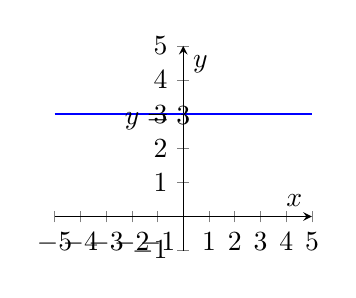
\begin{tikzpicture}
    % Graph for y = 3
    \begin{axis}[axis lines=middle, xlabel={$x$}, ylabel={$y$}, xtick={-5,-4,...,5}, ytick={-1,0,1,...,5}, domain=-5:5, samples=2, ymin=-1, ymax=5, xmin=-5, xmax=5, width=0.4\textwidth]
        \addplot [mark=none, blue, thick] coordinates {(-5,3) (5,3)};
        \node at (axis cs:-1,3.5) [anchor=north] {$y=3$};
    \end{axis}
\end{tikzpicture}
\hfill
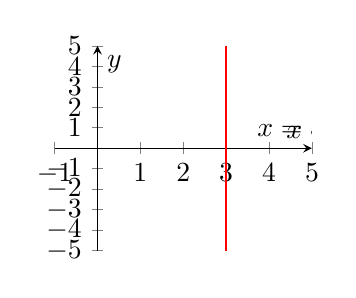
\begin{tikzpicture}
    % Graph for x = 3
    \begin{axis}[axis lines=middle, xlabel={$x$}, ylabel={$y$}, xtick={-1,0,1,...,5}, ytick={-5,-4,...,5}, domain=-5:5, samples=2, ymin=-5, ymax=5, xmin=-1, xmax=5, width=0.4\textwidth]
        \addplot [mark=none, red, thick] coordinates {(3,-5) (3,5)};
        \node at (axis cs:3.5,1) [anchor=west] {$x=3$};
    \end{axis}
\end{tikzpicture}
} {}{NOTAGS} 
 
 
 
 \ex
{\code{AxLx25x01x06x026}}{10}
{
\textbf{Graph the set of solutions of each equation.}

\begin{multicols}{3}
\begin{enumerate}
\item $y = -2$
\item $x = -2$
\end{enumerate}
\end{multicols}
} {

 

\begin{tikzpicture}
    % Axis for y = -2
    \begin{scope}[shift={(0,0)}]
        \draw[<->, thick] (-3,0) -- (3,0) node[right] {$x$};
        \draw[<->, thick] (0,-3) -- (0,3) node[above] {$y$};
        \draw[dashed,red,thick] (-3,-2) -- (3,-2);
        \node[right] at (3,-2) {$y = -2$};
    \end{scope}
    
    % Axis for x = -2
    \begin{scope}[shift={(8,0)}]
        \draw[<->, thick] (-3,0) -- (3,0) node[right] {$x$};
        \draw[<->, thick] (0,-3) -- (0,3) node[above] {$y$};
        \draw[dashed,blue,thick] (-2,-3) -- (-2,3);
        \node[above left] at (-2,3) {$x = -2$};
    \end{scope}
\end{tikzpicture}
} {}{NOTAGS} 
 
 
 
 \ex
{\code{AxLx25x01x06x027}}{10}
{
\textbf{Graph the set of solutions of each equation.}

\begin{multicols}{3}
\begin{enumerate}
\item $y = 0$
\item $x = 0$
\end{enumerate}
\end{multicols}
} {

 

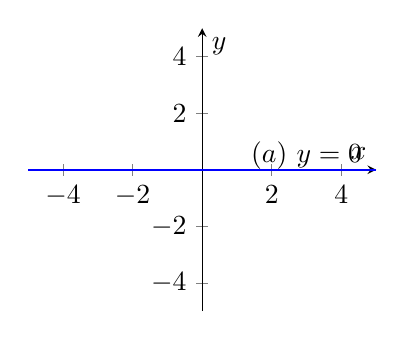
\begin{tikzpicture}
    \begin{axis}[
        width=6cm,
        axis lines=middle,
        xlabel={$x$},
        ylabel={$y$},
        ymin=-5, ymax=5,
        xmin=-5, xmax=5,
        ytick={-4,-2,2,4},
        xtick={-4,-2,2,4},
        domain=-5:5
      ]
      \addplot[domain=-5:5, samples=2, blue, thick] {0};
      \node at (axis cs: 3, 0.5) {$(a) \ y = 0$};
    \end{axis}
\end{tikzpicture}

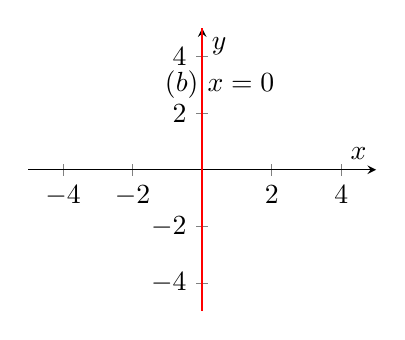
\begin{tikzpicture}
    \begin{axis}[
        width=6cm,
        axis lines=middle,
        xlabel={$x$},
        ylabel={$y$},
        ymin=-5, ymax=5,
        xmin=-5, xmax=5,
        ytick={-4,-2,2,4},
        xtick={-4,-2,2,4},
        domain=-5:5
      ]
      \addplot[domain=-5:5, samples=2, red, thick] ({0}, x);
      \node at (axis cs: 0.5, 3) {$(b) \ x = 0$};
    \end{axis}
\end{tikzpicture}
} {}{NOTAGS} 
 
 
 
 \ex
{\code{AxLx25x01x06x028}}{40}
{
Graph each equation.

\begin{multicols}{2}
\begin{enumerate}
\item $y = 3x + 1$
\item $y = 2x - 1$
\end{enumerate}
\end{multicols}
} {

 

\begin{center}
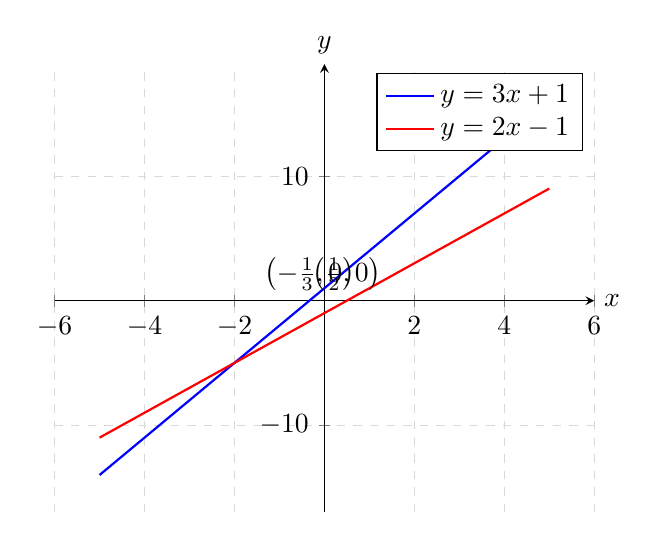
\begin{tikzpicture}
    \begin{axis}[
        axis lines = middle,
        xlabel = $x$,
        ylabel = $y$,
        enlargelimits,
        grid = both,
        grid style={dashed, gray!30},
        every axis y label/.style={at=(current axis.above origin),anchor=south},
        every axis x label/.style={at=(current axis.right of origin),anchor=west},
    ]
    % Plot for y = 3x + 1
    \addplot[
        domain=-5:5, 
        samples=100, 
        color=blue,
        thick
    ]
    {3*x + 1};
    \addlegendentry{$y = 3x + 1$}
    
    % Plot for y = 2x - 1
    \addplot[
        domain=-5:5, 
        samples=100, 
        color=red,
        thick
    ]
    {2*x - 1};
    \addlegendentry{$y = 2x - 1$}
    
    % Marking points on the graph
    \node[above] at (axis cs:-0.333,0) {$\left(-\frac{1}{3}, 0\right)$};
    \node[above] at (axis cs:0.5,0) {$\left(\frac{1}{2}, 0\right)$};
    
    \end{axis}
\end{tikzpicture}
\end{center}
} {}{NOTAGS} 
 
 
 
 \ex
{\code{AxLx25x01x06x029}}{40}
{
Graph each equation.

\begin{multicols}{2}
\begin{enumerate}
\item $y = \tfrac{1}{2}x + 2$
\item $y = -\tfrac{3}{2}x$
\end{enumerate}
\end{multicols}
} {

 

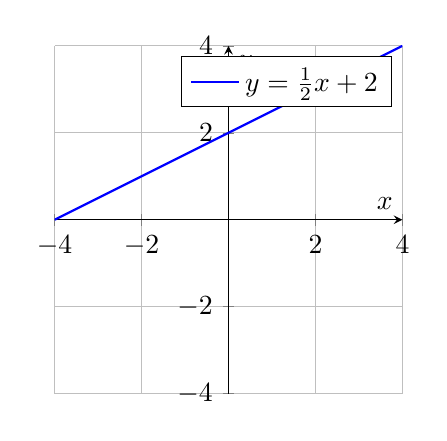
\begin{tikzpicture}
  % Graph y = 1/2x + 2
  \begin{axis}[
    axis lines = middle,
    xlabel = {$x$},
    ylabel = {$y$},
    ytick = {-4, -2, 0, 2, 4},
    xtick = {-4, -2, 0, 2, 4},
    xmin = -4, xmax = 4,
    ymin = -4, ymax = 4,
    legend pos = north east,
    grid = major,
    width = 6cm,
    height = 6cm
  ]
    \addplot[domain=-4:4, samples=100, smooth, thick, blue] {0.5*x + 2};
    \addlegendentry{$y = \tfrac{1}{2}x + 2$}
  \end{axis}
\end{tikzpicture}

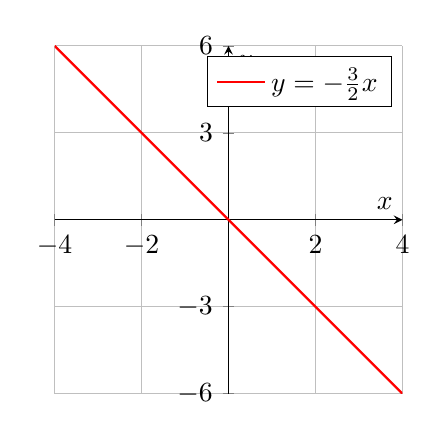
\begin{tikzpicture}
  % Graph y = -3/2x
  \begin{axis}[
    axis lines = middle,
    xlabel = {$x$},
    ylabel = {$y$},
    ytick = {-6, -3, 0, 3, 6},
    xtick = {-4, -2, 0, 2, 4},
    xmin = -4, xmax = 4,
    ymin = -6, ymax = 6,
    legend pos = north east,
    grid = major,
    width = 6cm,
    height = 6cm
  ]
    \addplot[domain=-4:4, samples=100, smooth, thick, red] {-1.5*x};
    \addlegendentry{$y = -\tfrac{3}{2}x$}
  \end{axis}
\end{tikzpicture}
} {}{NOTAGS} 
 
 
 
 \ex
{\code{AxLx25x01x06x030}}{40}
{
Graph each equation.

\begin{multicols}{2}
\begin{enumerate}
\item $y = 4$
\item $y = 4x$
\end{enumerate}
\end{multicols}
} {

 

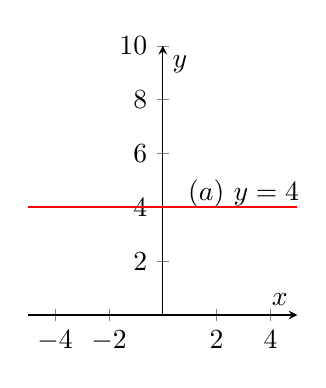
\begin{tikzpicture}
    % Graph for y = 4
    \begin{axis}[
        axis lines = middle, 
        xlabel = {$x$}, 
        ylabel = {$y$},
        ymin=0, ymax=10, 
        xmin=-5, xmax=5,
        width=5cm,
        height=5cm,
        domain=-5:5
    ]
    \addplot[samples=2,domain=-5:5,thick,red] {4};
    \node at (axis cs:3,4.5) {$(a)\ y=4$};
    \end{axis}
\end{tikzpicture}
\quad
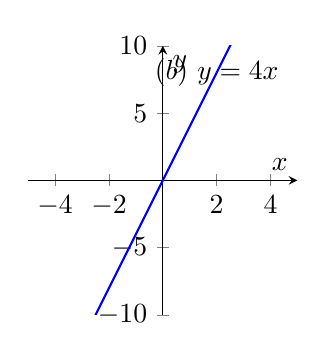
\begin{tikzpicture}
    % Graph for y = 4x
    \begin{axis}[
        axis lines = middle, 
        xlabel = {$x$}, 
        ylabel = {$y$},
        ymin=-10, ymax=10, 
        xmin=-5, xmax=5,
        width=5cm,
        height=5cm,
        domain=-5:5
    ]
    \addplot[domain=-5:5,thick,blue] {4*x};
    \node at (axis cs:2,8) {$(b)\ y=4x$};
    \end{axis}
\end{tikzpicture}
} {}{NOTAGS} 
 
 
 
 \ex
{\code{AxLx25x01x06x031}}{40}
{
Graph each equation.

\begin{multicols}{2}
\begin{enumerate}
\item $x = y + 3$
\item $x = 1$
\end{enumerate}
\end{multicols}
} {

 

The solutions for graphing the given equations are:

Equation (1) $x = y + 3$: 

The graph is a straight line with slope $1$, intersecting the $y$-axis at $-3$.

Equation (2) $x = 1$: 

The graph is a vertical line at $x = 1$.
} {}{NOTAGS} 
 
 
 
 \ex
{\code{AxLx25x01x06x032}}{40}
{
Graph each equation.

\begin{multicols}{2}
\begin{enumerate}
\item $y = -1$
\item $2x = 4y - 8$
\end{enumerate}
\end{multicols}
} {

 

$y = -1$ is a horizontal line through $y = -1$ on the Cartesian plane.

\begin{align*}
2x &= 4y - 8 \\
2x + 8 &= 4y \\
y &= \frac{2}{4}x + \frac{8}{4} \\
y &= \frac{1}{2}x + 2
\end{align*}

The line $y = \frac{1}{2}x + 2$ is a straight line with a slope of $\frac{1}{2}$ and a $y$-intercept at $2$.
} {}{NOTAGS} 
 
 
 
 \ex
{\code{AxLx25x01x06x033}}{30}
{
Graph the equation: $3x + 4y = 4$

} {

 

To graph the equation \(3x + 4y = 4\), follow these steps:

1. Solve for \(y\) in terms of \(x\):

\[
4y = -3x + 4
\]

\[
y = -\frac{3}{4}x + 1
\]

2. Identify the slope and y-intercept:

- Slope (\(m\)) is \(-\frac{3}{4}\).
- \(y\)-intercept is \(1\).

3. Plot the y-intercept \((0, 1)\).

4. Use the slope to find another point. From \((0, 1)\), move down 3 units and right 4 units to \((4, -2)\).

5. Draw the line through the points \((0, 1)\) and \((4, -2)\), extending in both directions.
} {}{NOTAGS} 
 
 
 
 \ex
{\code{AxLx25x01x15x015}}{10}
{
Graph the following function.

$f(x) = 2x + 1$
} {

 

To graph the function \( f(x) = 2x + 1 \), we follow these steps:

1. Identify the slope and y-intercept from the function \( f(x) = 2x + 1 \).

   - Slope: \( m = 2 \)
   - Y-intercept: \( b = 1 \)

2. Plot the y-intercept (0, 1) on the graph.

3. Use the slope \( m = 2 \) (rise over run) to determine another point. From (0, 1), move up 2 units and right 1 unit to point (1, 3).

4. Draw a line through these points to represent the function \( f(x) = 2x + 1 \).

Here is a basic sketch using LaTeX and TikZ:

\[
\begin{tikzpicture}[scale=1.0]
    \draw[thick,->] (-3,0) -- (3,0) node[right] {$x$}; % x-axis
    \draw[thick,->] (0,-1) -- (0,5) node[above] {$y$}; % y-axis
    \foreach \x in {-2,-1,1,2}
        \draw[thick] (\x,0.1) -- (\x,-0.1) node[below] {\small $\x$}; % x-ticks
    \foreach \y in {1,2,3,4}
        \draw[thick] (0.1,\y) -- (-0.1,\y) node[left] {\small $\y$}; % y-ticks
    \draw[thick,blue] (-2,-3) -- (3,7); % line f(x) = 2x + 1
    \node[blue] at (1,3.4) {\small $(1,3)$};
    \filldraw[blue] (0,1) circle (2pt);
    \node[blue] at (0.3,1) {\small $(0,1)$};
\end{tikzpicture}
\]
} {}{NOTAGS} 
 
 
 
 \ex
{\code{AxLx25x01x15x016}}{30}
{
Graph the following function.

$g(x) = 2x$
} {

 

To graph the function \( g(x) = 2x \), we first note that this is a linear function in the form \( y = mx + b \), where \( m = 2 \) and \( b = 0 \).

The graph is a straight line passing through the origin. The slope \( m = 2 \) indicates that for each unit increase in \( x \), \( g(x) \) increases by 2 units.

To create the graph, we will plot two points:

1. When \( x = 0 \), \( g(0) = 2 \times 0 = 0 \). Thus, the point is \( (0, 0) \).
2. When \( x = 1 \), \( g(1) = 2 \times 1 = 2 \). Thus, the point is \( (1, 2) \).

\[
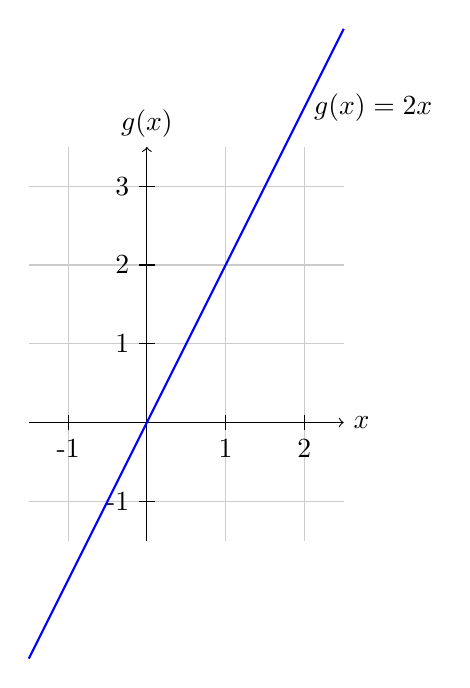
\begin{tikzpicture}[scale=1.0]
    \draw[thin, gray!40] (-1.5, -1.5) grid (2.5, 3.5);
    \draw[->] (-1.5, 0) -- (2.5, 0) node[right] {$x$};
    \draw[->] (0, -1.5) -- (0, 3.5) node[above] {$g(x)$};
    \foreach \x in {-1, 1, 2} \draw (\x, 0.1) -- (\x, -0.1) node[below] {\x};
    \foreach \y in {-1, 1, 2, 3} \draw (0.1, \y) -- (-0.1, \y) node[left] {\y};
    \draw[thick, blue] (-1.5, -3) -- (2.5, 5);
    \node at (2,4) [right,black] {$g(x) = 2x$};
\end{tikzpicture}
\]
} {}{NOTAGS} 
 
 
 
 \ex
{\code{AxLx25x01x15x017}}{30}
{
Graph the following function.

$h(x) = \tfrac12 x + 1$
} {

 

\[
\text{The graph of } h(x) = \frac{1}{2}x + 1 \text{ is a straight line.}
\]

\text{The slope of the line is } $\frac{1}{2}$ \text{ and the y-intercept is } 1.

\[
\text{To graph the function, plot the y-intercept at } (0, 1).
\]

\text{From the y-intercept, use the slope to find another point:}

\[
\text{From } (0, 1) \text{, go up 1 and to the right 2 to reach the point } (2, 2).
\]

\text{Draw a straight line through the points } (0, 1) \text{ and } (2, 2).

\[
\text{The line extends infinitely in both directions.}
\]
} {}{NOTAGS} 
 
 
 
 \ex
{\code{AxLx25x01x15x018}}{30}
{
Graph the following function.

$f(x) = -2x + 3$
} {

 

To graph the function \( f(x) = -2x + 3 \), follow these steps:

1. Identify the y-intercept: When \( x = 0 \),
   \[
   f(0) = -2(0) + 3 = 3.
   \]
   So, the y-intercept is \( (0, 3) \).

2. Identify the slope: The slope \( m \) is -2, which means for every unit increase in \( x \), \( f(x) \) decreases by 2 units.

3. Find another point: Using the slope, from the y-intercept \( (0, 3) \), move 1 unit to the right (\( x = 1 \)) and 2 units down:
   \[
   f(1) = -2(1) + 3 = 1.
   \]
   So, another point is \( (1, 1) \).

4. Plot the points: Plot the points \( (0, 3) \) and \( (1, 1) \) on the Cartesian plane.

5. Draw the line: Connect the points with a straight line, extending in both directions.

\[
\begin{array}{c}
\text{Graph of } f(x) = -2x + 3 \text{ with points and slope} \\
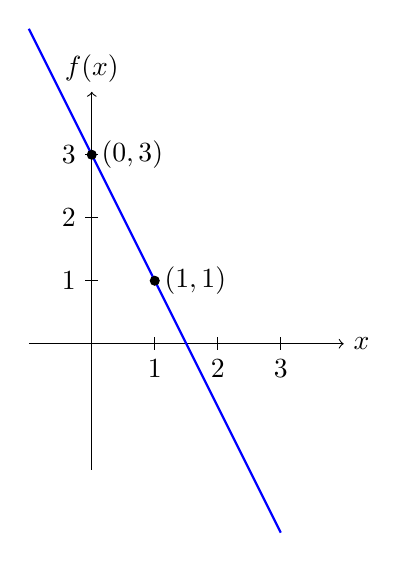
\begin{tikzpicture}[scale=0.8]
    \draw[->] (-1, 0) -- (4, 0) node[right] {\(x\)};
    \draw[->] (0, -2) -- (0, 4) node[above] {\(f(x)\)};
    \foreach \x in {1, 2, 3} \draw (\x,0.1) -- (\x,-0.1) node[below] {\(\x\)};
    \foreach \y in {1, 2, 3} \draw (0.1,\y) -- (-0.1,\y) node[left] {\(\y\)};
    \draw[thick,blue] plot[smooth] coordinates{(-1,5)(0,3)(1,1)(2,-1)(3,-3)};
    \filldraw[black] (0,3) circle (2pt) node[anchor=west]{\((0,3)\)};
    \filldraw[black] (1,1) circle (2pt) node[anchor=west]{\((1,1)\)};
\end{tikzpicture}
\end{array}
\]
} {}{NOTAGS} 
 
 
 
 \ex
{\code{AxLx25x01x15x019}}{10}
{
Graph the following function.

$f(x) = -2x - 3$
}
{

 

$f(x) = -2x - 3$

To graph the function, identify the slope and y-intercept:

- Slope: $-2$
- Y-intercept: $(0, -3)$

Follow these steps to plot the graph:

1. Plot the y-intercept $(0, -3)$ on the coordinate plane.
2. Use the slope $-2$, which means a rise of $-2$ and a run of $1$, to find another point. Starting from $(0, -3)$, move down 2 units and 1 unit to the right to find another point $(1, -5)$.
3. Draw a straight line through these points to graph the function. 

The graph is a straight line with a downward slope passing through $(0, -3)$ and $(1, -5)$.
} {}{NOTAGS}

\ex
{\code{AxLx25x01x21x009}}{30}
{
Let \(f(x)=4x-3\). Find the slope and all intercepts. Then graph \(f\).
}
{

 

The slope of \(f(x) = 4x - 3\) is the coefficient of \(x\), which is 4.

The y-intercept is found by setting \(x = 0\):

\[
f(0) = 4(0) - 3 = -3
\]

Thus, the y-intercept is \((0, -3)\).

The x-intercept is found by setting \(f(x) = 0\):

\[
4x - 3 = 0
\]

\[
4x = 3
\]

\[
x = \frac{3}{4}
\]

Thus, the x-intercept is \(\left(\frac{3}{4}, 0\right)\).

To graph \(f(x)\), plot the intercepts \((0, -3)\) and \(\left(\frac{3}{4}, 0\right)\), and use the slope 4 (rise over run: 4/1) to draw the line passing through these points.
} {}{NOTAGS}


\ex
{\code{AxLx25x01x21x005}}{25}
{
Consider two linear functions \(f(x)=-2x+1\) and \(g(x)=2x+1\).

\begin{multicols}{2}
\begin{enumerate}
\item Find the intersection point of \(f\) and \(g\).
\item Give an example of a linear function \(h(x)\) that does not intersect \(f(x)\). Justify.
\end{enumerate}
\end{multicols}
}
{

 

1. To find the intersection point of \(f(x) = -2x + 1\) and \(g(x) = 2x + 1\), set them equal to each other:

\[
-2x + 1 = 2x + 1
\]

Subtract \(1\) from both sides:

\[
-2x = 2x
\]

Move all \(x\) terms to one side:

\[
-2x - 2x = 0
\]

\[
-4x = 0
\]

Divide by \(-4\):

\[
x = 0
\]

Substitute \(x = 0\) back into either equation to find \(y\):

\[
f(0) = -2(0) + 1 = 1
\]

The intersection point is \((0, 1)\).

2. A linear function \(h(x)\) that does not intersect \(f(x)\) can have the same slope but a different intercept. Since \(f(x)\) has a slope of \(-2\), let \(h(x) = -2x + c\), where \(c \neq 1\).

Example: Choose \(c = 2\). Then \(h(x) = -2x + 2\).

Justification: \(h(x) = -2x + 2\) is parallel to \(f(x)\) because they have the same slope. Thus, they do not intersect, as they have different \(y\)-intercepts.
} {}{NOTAGS}


\ex
{\code{AxLx25x02x12x001}}{15}
{
Find the intersection point of the two linear functions \(f(x)=-5x+1\) and \(h(x)=-5x -12\).

}
{

 

To find the intersection point of the functions \( f(x) = -5x + 1 \) and \( h(x) = -5x - 12 \), set the two functions equal to each other:

\[
-5x + 1 = -5x - 12
\]

To solve for \( x \), add \( 5x \) to both sides:

\[
1 = -12
\]

This simplifies to a contradiction, which means the lines are parallel and do not intersect. Therefore, there is no intersection point.
} {}{NOTAGS}


\ex
{\code{AxLx25x02x12x002}}{15}
{
Find the linear function such that $f(-1) = 4$ and $f(5) = 1$.

}
{

 

The linear function can be written in the form \( f(x) = mx + b \).

We have two points: \((-1, 4)\) and \( (5, 1) \).

First, compute the slope \( m \):

\[
m = \frac{f(5) - f(-1)}{5 - (-1)} = \frac{1 - 4}{5 + 1} = \frac{-3}{6} = -\frac{1}{2}
\]

Now use the point-slope form to find \( b \) using point \((-1, 4)\):

\[
4 = -\frac{1}{2}(-1) + b 
\]
\[
4 = \frac{1}{2} + b
\]
\[
b = 4 - \frac{1}{2} = \frac{8}{2} - \frac{1}{2} = \frac{7}{2}
\]

Thus, the linear function is:

\[
f(x) = -\frac{1}{2}x + \frac{7}{2}
\]
} {}{NOTAGS}

\ex
{\code{AxLx25x02x12x003}}{15}
{
Find the linear function such that $f(2) = 0.5$ and $f(0) = 0$.

}
{

 

Given that $f(x)$ is a linear function, it can be expressed in the form $f(x) = mx + b$.

We have the conditions:
1. $f(2) = 0.5$
2. $f(0) = 0$

First, using $f(0) = 0$, we find that:
\[ 
m \cdot 0 + b = 0 \implies b = 0 
\]

Thus, the function simplifies to:
\[ 
f(x) = mx 
\]

Next, use the condition $f(2) = 0.5$:
\[ 
m \cdot 2 = 0.5 \implies m = \frac{0.5}{2} = 0.25 
\]

Therefore, the linear function is:
\[ 
f(x) = 0.25x 
\]
} {}{NOTAGS}



\ex
{\code{AxLx25x02x03x001}}{30}
{
 Find the equation of the line passing through the point $(1,3)$ that is parallel to the line with equation $3x + 2y = 5$.
}
{

\vspace{3mm}
SOLUTION:
If the line we want is parallel to $3x + 2y = 5$, it must have the same slope. 

To find the slope of $3x + 2y = 5$, solve for $y$ and then the slope will be the coefficient of $x$: $3x + 2y = 5 \ \rightarrow \ 2y = -3x + 5\ \rightarrow y = -\frac{3}{2}x + \frac{5}{2}$. Thus the slope (of both lines) is $m=-\frac{3}{2}.$

Therefore the equation of the line we want is $y-3 = -\frac{3}{2}(x-1)$ (use point-slope form).
} {}{NOTAGS}



\ex
{\code{AxLx25x02x12x004}}{10}
{
Determine whether the lines are parallel, perpendicular, or neither.

\begin{multicols}{2}
\begin{enumerate}

\item
$y = 3x + 1$

\item
$y = 30x + 1$

\end{enumerate}
\end{multicols}

}
{

 

The slopes of the lines are given by the coefficients of \(x\) in the equations of the lines. 

For line 1, the equation is:
\[ 
y = 3x + 1 
\]
The slope is \(3\).

For line 2, the equation is:
\[ 
y = 30x + 1 
\]
The slope is \(30\).

To determine if the lines are parallel, we check if their slopes are equal. To determine if they are perpendicular, we check if the product of their slopes is \(-1\).

Parallel: \(3 \neq 30\)

Perpendicular: \(3 \times 30 = 90 \neq -1\)

Thus, the lines are neither parallel nor perpendicular.
} {}{NOTAGS}


\ex
{\code{AxLx25x02x12x005}}{10}
{
Determine whether the lines are parallel, perpendicular, or neither.

\begin{multicols}{2}
\begin{enumerate}

\item
$y + 5x = 1$

\item
$y = -5x + 19$

\end{enumerate}
\end{multicols}

}
{

 

The given lines are:

1. \( y + 5x = 1 \)
2. \( y = -5x + 19 \)

Convert the first line to slope-intercept form:

\[
y + 5x = 1 \implies y = -5x + 1
\]

Now both lines are in slope-intercept form:

1. \( y = -5x + 1 \)
2. \( y = -5x + 19 \)

Both lines have the same slope \(-5\). Therefore, the lines are parallel.
} {}{NOTAGS}

\ex
{\code{AxLx25x02x12x105}}{10}
{
Determine whether the lines are parallel, perpendicular, or neither.

\begin{multicols}{2}
\begin{enumerate}

\item
$2y + 4x = 1$

\item
$8y = 4x + 10$

\end{enumerate}
\end{multicols}

}
{

 

To determine whether the lines are parallel, perpendicular, or neither, we need to find the slopes of the lines from their equations.

For the first line: \(2y + 4x = 1\)

Convert to slope-intercept form \(y = mx + b\):

\[ 2y = -4x + 1 \]

\[ y = -2x + \frac{1}{2} \]

The slope (\(m\)) is \(-2\).

For the second line: \(8y = 4x + 10\)

Convert to slope-intercept form:

\[ y = \frac{1}{2}x + \frac{5}{4} \]

The slope (\(m\)) is \(\frac{1}{2}\).

Now we compare the slopes:

\[
-2 \quad \text{and} \quad \frac{1}{2}
\]

The lines are neither parallel nor perpendicular because the slopes are not equal (parallel lines have equal slopes) and their product is not \(-1\) (perpendicular lines have slopes whose product is \(-1\)).

Thus, the lines are neither parallel nor perpendicular.
} {}{NOTAGS}


\ex
{\code{AxLx25x02x12x006}}{10}
{
Consider the linear equation $f(x) = (3/2)x - 6$.
Find the slope of a line parallel to $f$.
Find the slope of a line perpendicular to $f$.

}
{

 

The slope of the line given by the equation \( f(x) = \frac{3}{2}x - 6 \) is \(\frac{3}{2}\).

The slope of a line parallel to \( f(x) \) is also \(\frac{3}{2}\).

The slope of a line perpendicular to \( f(x) \) is the negative reciprocal of \(\frac{3}{2}\), which is \(-\frac{2}{3}\).
} {}{NOTAGS}

\ex
{\code{AxLx25x02x12x007}}{10}
{
Consider the linear equation $f(x) = -6x$.
Find the slope of a line parallel to $f$.
Find the slope of a line perpendicular to $f$.

}
{

 

The slope of a line parallel to $f(x) = -6x$ is $-6$.

The slope of a line perpendicular to $f(x) = -6x$ is $\frac{1}{6}$.
} {}{NOTAGS}


\ex
{\code{AxLx25x02x12x010}}{25}
{
Write down the linear function whose graph is parallell to
the linear function
$g(x) = 3x -1$ and passing through the point $(4, 9)$.
}
{

 

The linear function parallel to $g(x) = 3x - 1$ has the same slope, which is $3$. Therefore, its equation is in the form $f(x) = 3x + b$. To find $b$, use the point $(4, 9)$:

\[
9 = 3(4) + b
\]

\[
9 = 12 + b
\]

\[
b = 9 - 12 = -3
\]

Thus, the linear function is:

\[
f(x) = 3x - 3
\]
} {}{NOTAGS}

\ex
{\code{AxLx25x02x12x011}}{25}
{
Write down the equation for the line parallel to
$h(t) = 3t - 9$ and passing through the point $(0, 0)$.
}
{

 

The line parallel to $h(t) = 3t - 9$ will have the same slope. The slope of $h(t)$ is 3.

The equation of a line with slope $m$ passing through a point $(x_1, y_1)$ is given by:

\[ y - y_1 = m(x - x_1) \]

Using the point $(0, 0)$ and the slope 3:

\[ y - 0 = 3(x - 0) \]

\[ y = 3x \]
} {}{NOTAGS}


\ex
{\code{AxLx25x02x12x008}}{25}
{
Write an equation for a line perpendicular to
$f(x) = 3x + 4$ and passing through the point $(3, 1)$.
}
{

 

Given that the slope of the line $f(x) = 3x + 4$ is 3, the slope of a line perpendicular to it is the negative reciprocal: $-1/3$. 

To find the equation of the line passing through the point $(3, 1)$ with this slope, we use the point-slope form:

\[
y - y_1 = m(x - x_1)
\]

Substituting $m = -\frac{1}{3}$ and the point $(3, 1)$:

\[
y - 1 = -\frac{1}{3}(x - 3)
\]

Simplifying:

\[
y - 1 = -\frac{1}{3}x + 1
\]

\[
y = -\frac{1}{3}x + 2
\]
} {}{NOTAGS}

\ex
{\code{AxLx25x02x12x009}}{25}
{
Write an equation for a line perpendicular to
$f(x) = -2x + 4$ and passing through the point $(-4, -1)$.
}
{

 

A line perpendicular to the line $f(x) = -2x + 4$ will have a slope that is the negative reciprocal of $-2$. Thus, the slope of the perpendicular line is $\frac{1}{2}$.

We use the point-slope form of a line $y - y_1 = m(x - x_1)$ where $(x_1, y_1)$ is the point $(-4, -1)$ and $m$ is the slope $\frac{1}{2}$:

\[
y - (-1) = \frac{1}{2}(x - (-4))
\]

Simplifying gives:

\[
y + 1 = \frac{1}{2}(x + 4)
\]

\[
y + 1 = \frac{1}{2}x + 2
\]

Subtracting 1 from both sides, we get the equation of the line:

\[
y = \frac{1}{2}x + 1
\]
} {}{NOTAGS}


\ex
{\code{AxLx25x02x12x012}}{25}
{
Find the point of intersection between the lines, if it exists:

$2x - 3y = 12$ and $5y + x = 30$.
}
{

 

To find the point of intersection, solve the system of equations:

\[ 2x - 3y = 12 \]

\[ 5y + x = 30 \]

First, solve the second equation for \(x\):

\[ x = 30 - 5y \]

Substitute \(x = 30 - 5y\) into the first equation:

\[ 2(30 - 5y) - 3y = 12 \]

\[ 60 - 10y - 3y = 12 \]

\[-13y = 12 - 60\]

\[-13y = -48\]

\[ y = \frac{48}{13} \]

Now substitute \(y = \frac{48}{13}\) back into the expression for \(x\):

\[ x = 30 - 5\left(\frac{48}{13}\right) \]

\[ x = 30 - \frac{240}{13} \]

Convert 30 into a fraction with the denominator 13:

\[ x = \frac{390}{13} - \frac{240}{13} \]

\[ x = \frac{150}{13} \]

Thus, the point of intersection is:

\(\left(\frac{150}{13}, \frac{48}{13}\right)\)
} {}{NOTAGS}

\ex
{\code{AxLx25x02x12x013}}{25}
{
Find the point of intersection between the lines, if it exists:

$f(x) = x  + 1$ and $g(x) = 2x - 1$.
}
{

 

To find the point of intersection between the lines \( f(x) = x + 1 \) and \( g(x) = 2x - 1 \), we set the two equations equal to each other and solve for \( x \):

\[
x + 1 = 2x - 1
\]

Subtract \( x \) from both sides:

\[
1 = x - 1
\]

Add 1 to both sides:

\[
2 = x
\]

Now, substitute \( x = 2 \) back into either equation to find \( y \). Using \( f(x) = x + 1 \):

\[
f(2) = 2 + 1 = 3
\]

Thus, the point of intersection is:

\((2, 3)\)
} {}{NOTAGS}


\ex
{\code{AxLx25x02x12x015}}{50}
{
Consider two kinds of gym membership plans.

\begin{itemize}
    \item Platinum Plan: \$20 per month + \$3 per fitness class.
    \item Gold Plan: \$10 per month + \$6 per fitness class.
\end{itemize}

Which plan is better if you attend 2 classes a month? Which plan is better if you attend 5 classes a month?

How many classes must you attend in a month for  the Platinum plan to save you money?
}
{

 

Let \( x \) be the number of fitness classes attended in a month.

For the Platinum Plan:
\[
C_P(x) = 20 + 3x
\]

For the Gold Plan:
\[
C_G(x) = 10 + 6x
\]

**Case 1: 2 classes per month**

Platinum Plan cost:
\[
C_P(2) = 20 + 3 \times 2 = 26
\]

Gold Plan cost:
\[
C_G(2) = 10 + 6 \times 2 = 22
\]

For 2 classes per month, the Gold Plan is better.

**Case 2: 5 classes per month**

Platinum Plan cost:
\[
C_P(5) = 20 + 3 \times 5 = 35
\]

Gold Plan cost:
\[
C_G(5) = 10 + 6 \times 5 = 40
\]

For 5 classes per month, the Platinum Plan is better.

**Finding when the Platinum Plan saves money**

Set \( C_P(x) < C_G(x) \):

\[
20 + 3x < 10 + 6x
\]

Simplifying:
\[
20 < 10 + 3x
\]

\[
10 < 3x
\]

\[
x > \frac{10}{3}
\]

Since \( x \) must be a whole number, \( x \geq 4 \).

Therefore, you must attend at least 4 classes per month for the Platinum plan to save you money.
} {}{NOTAGS}


\ex
{\code{AxLx25x02x12x016}}{50}
{
Suppose you want to rent a car, and these are your options.

\begin{itemize}
    \item Option 1: \$25 per day + \$0.10 per mile.
    \item Option 2: \$35 per day + \$0.05 per mile.
\end{itemize}

 How many miles do you need to drive in a day for option 2 to be the cheaper?
}
{

 

Let $m$ be the number of miles driven in a day. 

The cost of option 1 is given by:
\[ C_1 = 25 + 0.10m \]

The cost of option 2 is given by:
\[ C_2 = 35 + 0.05m \]

We want to find the value of $m$ for which option 2 is cheaper than option 1. Therefore, we solve the inequality:
\[ 35 + 0.05m < 25 + 0.10m \]

Subtract $25$ from both sides:
\[ 10 + 0.05m < 0.10m \]

Subtract $0.05m$ from both sides:
\[ 10 < 0.05m \]

To isolate $m$, divide both sides by $0.05$:
\[ m > \frac{10}{0.05} \]

Calculate:
\[ m > 200 \]

Therefore, you need to drive more than 200 miles in a day for option 2 to be the cheaper choice.
} {}{NOTAGS}



\ex
{\code{AxLx25x02x12x014}}{40}
{
 A cell phone company
offers two plans.

Plan A: \$20 per month and
\$1 for every one hundred
texts.

Plan B: \$50 per month with
free unlimited texts.

How many texts would you
need to send per month
for plan B to save you
money?
}
{

 

Let the number of texts sent per month be \( x \).

For Plan A:

\[
\text{Cost of Plan A} = 20 + \frac{x}{100}
\]

For Plan B:

\[
\text{Cost of Plan B} = 50
\]

Set the cost of Plan A greater than the cost of Plan B for savings:

\[
20 + \frac{x}{100} > 50
\]

Subtract 20 from both sides:

\[
\frac{x}{100} > 30
\]

Multiply both sides by 100:

\[
x > 3000
\]

Thus, you need to send more than 3000 texts per month for Plan B to save you money.
} {}{NOTAGS}



\ex
{\code{AxLx25x02x12x115}}{40}
{
 A cell phone company
offers two plans.

Plan A: \$15 per month and
\$2 for every 300
texts.

Plan B: \$25 per month and \$0.50 for every 100 texts.

How many texts would you
need to send per month
for plan B to save you
money?
}
{

 

Let \( x \) be the number of texts sent per month.

Cost of Plan A: 
\[
C_A = 15 + 2 \left\lceil \frac{x}{300} \right\rceil
\]

Cost of Plan B:
\[
C_B = 25 + 0.5 \left\lceil \frac{x}{100} \right\rceil
\]

We want Plan B to be cheaper:
\[
C_B < C_A
\]

Substitute the costs:
\[
25 + 0.5 \left\lceil \frac{x}{100} \right\rceil < 15 + 2 \left\lceil \frac{x}{300} \right\rceil
\]

Simplify:
\[
10 + 0.5 \left\lceil \frac{x}{100} \right\rceil < 2 \left\lceil \frac{x}{300} \right\rceil
\]

Multiply the entire inequality by 6 to clear denominators:
\[
60 + 3 \left\lceil \frac{x}{100} \right\rceil < 12 \left\lceil \frac{x}{300} \right\rceil
\]

Use \(\left\lceil \frac{x}{100} \right\rceil \approx \frac{x}{100}\) and \(\left\lceil \frac{x}{300} \right\rceil \approx \frac{x}{300}\) for approximation:
\[
60 + 3 \frac{x}{100} < 12 \frac{x}{300}
\]

Simplify:
\[
60 + \frac{3x}{100} < \frac{4x}{100}
\]

Rewriting gives:
\[
60 < \frac{x}{100}
\]

Multiplying by 100:
\[
6000 < x
\]

Thus, you need to send more than 6000 texts per month for Plan B to save you money.
} {}{NOTAGS}



\ex
{\code{AxLx25x02x12x017}}{50}
{
Suppose a city's population has been decreasing at a constant rate of 
50 people a year.  
\begin{enumerate}

\item
If the population is now 400, what will the population be in 2 years?

\item 
When will it be a ghost town (that is, when will the population be zero)?

\item 
Write down a function $P(t)$  which models the population.


\end{enumerate}

}
{

 

The city's population is decreasing at a rate of 50 people per year. We can express this as a linear function of time.

1. If the population is now 400, what will the population be in 2 years?

The population after 2 years can be calculated as follows:

\[ 
P(2) = 400 - 2 \times 50 = 400 - 100 = 300 
\]

2. When will it be a ghost town (that is, when will the population be zero)?

We need to solve for \( t \) when the population \( P(t) \) is zero:

\[
0 = 400 - 50t 
\]

Solving for \( t \):

\[
50t = 400 
\]

\[
t = \frac{400}{50} = 8 
\]

Thus, the city will become a ghost town in 8 years.

3. Write down a function \( P(t) \) which models the population.

The function \( P(t) \) modeling the population is:

\[
P(t) = 400 - 50t 
\]
} {}{NOTAGS}



\ex
{\code{AxLx25x02x12x018}}{50}
{
Suppose a city's population in 2020 was 4005, has been increasing at a constant rate of 
35 people a year.  
\begin{enumerate}

\item 
Write down a function $P(t)$  which models the population.

\item
Use your model to predict the population in the year 2030.

\item
Use your model to predict the population 7.2 years after 2020? (use a calculator if you have one, or leave your answer unevaluated)



\end{enumerate}

}
{

 

$P(t) = 4005 + 35t$

For the year 2030, $t = 2030 - 2020 = 10$.

$P(10) = 4005 + 35 \times 10 = 4005 + 350 = 4355$

For 7.2 years after 2020, $t = 7.2$.

$P(7.2) = 4005 + 35 \times 7.2 = 4005 + 252 = 4257$
} {}{NOTAGS}



\ex
{\code{AxLx25x02x12x019}}{50}
{
Suppose a child's weight fom ages 1 to age 5 is modeled by the following equation:
$W(t) = 11 + 6t$
\begin{enumerate}

\item 
How much does the child weigh at age 3? And at 3 and a half?

\item 
How much weight does the child gain each year?

\item 
What does the model say about the child's weight at age 9?


\end{enumerate}

}
{

 

$W(3) = 11 + 6 \times 3 = 11 + 18 = 29$

$W\left(3.5\right) = 11 + 6 \times 3.5 = 11 + 21 = 32$

The child gains $6$ units of weight each year.

At age 9: $W(9) = 11 + 6 \times 9 = 11 + 54 = 65$
} {}{NOTAGS}





\ex
{\code{AxLx25x02x12x020}}{50}
{
Suppose that the number of people in a town who have a cold grows
at a constant rate.  In December 100 people have the cold, and a month later, 120 poeple have a cold.
\begin{enumerate}

\item 
How many people have a cold in March?

\item 
Write down an equation which models this situation.


\end{enumerate}

}
{

 

\item In December, 100 people have a cold. In January, 120 people have a cold. The increase each month is:

\[
\frac{120 - 100}{1} = 20 \text{ people per month}
\]

Therefore, in February, there are \(120 + 20 = 140\) people with a cold, and in March, there are \(140 + 20 = 160\) people with a cold.

\item Let \(C(t)\) be the number of people with a cold \(t\) months after December. The equation for this linear growth is:

\[
C(t) = 100 + 20t
\]
} {}{NOTAGS}




\ex
{\code{AxLx25x02x12x021}}{50}
{
Suppose we have a scatter plot of some data comparing hours spent studying
with grade on an exam, where hours (t) is the independent variable.  
Suppose the best-fit line turns out to be this:
$G(t) = 20 + 15t$
\begin{enumerate}

\item 
According to this best fit line, what will your grade be if you do not study at all?

\item 
How much do you need to study to get 100?


\end{enumerate}

}
{

 

\begin{enumerate}

\item 
If you do not study at all, $t = 0$. Therefore, 
\[
G(0) = 20 + 15 \times 0 = 20.
\]
Your grade will be 20.

\item 
To get a grade of 100, set $G(t) = 100$:
\[
100 = 20 + 15t.
\]
Solving for \(t\):
\[
100 - 20 = 15t \\
80 = 15t \\
t = \frac{80}{15} = \frac{16}{3}.
\]
You need to study approximately \( \frac{16}{3} \) hours, or about 5.33 hours.

\end{enumerate}
} {}{NOTAGS}


\ex
{\code{TESTxxxAxLx25x03x26x001}}{40}
{
Consider the linear function \(f(x)=-2x + 4\). Find its slope and all its intercepts. Then graph \(f\).
}
{

\solfig{TESTxxxAxLx25x03x26x001}

} {}{NOTAGS}


\ex
{\code{AxLx25x10x27x001}}{40}
{
Consider the linear function \(f(x)=-3x + 2\). Find its slope and all its intercepts. Then graph \(f\).
}
{

SOLUTION:

It is in $mx +b$ form with $m = -3$ and $b = 2$, so:

Slope is $-3$

$y$-intercept is 2.

For $x$-intercepts: Solve $-3x + 2 =0$.
Subtract 2 to get $-3x = -2$, then divide by $-3$ to get $x = \frac{2}{3}$.

Graph:
\vspace{25mm}


} {}{type: TEST}



\ex
{\code{TESTxxxAxLx25x03x26x002}}{35}
{
Find the point of intersection between the lines, if it exists:

$f(x) = \dfrac{2}{3}x  - 2$ and $g(x) = -\dfrac{1}{3}x + 1$.
}
{

SOLUTION:
\vspace{2mm}

$
\begin{array}{ccc}
\dfrac{2}{3}x - 2 & = & -\dfrac{1}{3}x + 1 \\
2x - 6 & = & -x + 3 \\
3x & = & 9 \\
x & = & 3 \\
\end{array}
$

To find $y$, use either equation, say:
$y = \dfrac{2}{3}(3) - 2 = 0$,
thus the point of intersection is $(3, 0)$.

} {}{NOTAGS}


\ex
{\code{TESTxxxAxLx26x03x22x004}}{35}
{
Find the point of intersection between the lines, if it exists:

$h(x) = 7x  + 2$ and $g(x) = 4x - 10$.
}
{

SOLUTION:
\vspace{2mm}

$
\begin{array}{ccc}
7x + 2 & = & 4x - 10 \\
3x & = & -12 \\
x & = & -4 \\
\end{array}
$

To find $y$, use either equation, say:
$y = 7(-4) + 2 = -26$,
thus the point of intersection is $(-4, -26)$.

} {}{type: TEST}



\ex
{\code{TESTxxxAxLx25x03x26x003}}{20}
{
Consider the linear equation $f(x) = \dfrac{4}{3}x - 12$.

\begin{multicols}{2}
\begin{enumerate}
\item Write down the equation for any line that does not intersect $f$.
\item Find the slope of a line perpendicular to $f$.
\end{enumerate}
\end{multicols}

}
{

SOLUTION:

For (a): Any $g(x) = \dfrac{4}{3}x + k$, where $k$ is any number besides $-12$,
since then $g$ is a parallel line to $f$ (since they both have slope $4/3$), but they are distinct lines since they have different $y$-intercepts.

\vspace{3mm}

For (b): $-\dfrac{3}{4}$, since $f$ has slope $4/3$, so the slope of a perpendicular line takes $4/3$, negates it, and takes its reciprocal.

} {}{NOTAGS}


\ex
{\code{TESTxxxAxLx25x04x28x001}}{45}
{ Consider the linear equation $f(x) = 3x - 1$.

\begin{multicols}{2}
\begin{enumerate}
\item Write the equation for a line parallel to $f(x)$ and passing through the point $(-2, 7)$.

\item Write the equation for a line perpendicular to $f(x)$ and passing through the point $(0, -5)$.

\end{enumerate}
\end{multicols} 

}
{

SOLUTION:

\begin{enumerate}
\item To be parallel, the slope is 3.  Using the point $(-2, 7)$ and the point-slope form of the line we get:
$y = 7 + 3(x - (-2))$ which simplifies to $y = 7 + 3(x + 2)$ or even
$y = 3x + 13$

\vspace{3mm}

\item To be perpendicular, the slope is $-\frac{1}{3}$.  Using the point  $(0, -5)$
 and the point-slope form of the line we get:
 $y = -5 + -\frac{1}{3}(x - 0)$ which simplifies to $y =-\frac{1}{3}x - 5$

\end{enumerate}

} {}{type: TEST}



\ex
{\code{GROUPxAxLx25x02x12x001}}{80}
{
The following data from a US Census report indicates for various years,
the percentage of the population (who are 25 years or older) with a college degree.

\begin{table}[H]
    \begin{tabular}{l| l| l| l| l| l|  l|}

     $Year$  & $1990$ 
           & $1992$ 
           & $1994$ 
           & $1996$ 
           & $1998$ 
           & $2000$ 
\\
      \hline

     $Graduate \ \%$  & $21.3$ 
               & $21.4$ 
               & $22.2$ 
               & $23.6$ 
               & $24.4$ 
               & $25.6$
\\
      \hline
    \end{tabular}
\end{table}

\begin{enumerate}

\item 
Use google sheets to find the equation of a best-fit line for this data.
Make a rough sketch of the scatter diagram along with the best-fit line on top of it.

\item 
Use your model to guess what the percent of college graduates was in the year 1995?
(this is interpolation ...)

\item
Use your model to guess what the percent of college graduates was in the year 2025?
(this is predication ...).  Wonder if the prediction is correct??


\end{enumerate}

}
{

 

1. The equation of the best-fit line, determined using Google Sheets, is:

   $y = 0.7225x - 1442.65$, 

   where $x$ is the year and $y$ is the percentage of graduates. Below is a rough sketch representation:
\junk{
   \[
   \begin{tikzpicture}
       \begin{axis}[
           xlabel={Year},
           ylabel={Graduate \%},
           xmin=1990, xmax=2000,
           ymin=21, ymax=26,
           xtick={1990,1992,1994,1996,1998,2000},
           ytick={21,22,23,24,25,26},
           ymajorgrids=true,
           grid style=dashed,
       ]
       \addplot[
           scatter,only marks,scatter src=explicit symbolic
       ] coordinates {
           (1990,21.3) [a]
           (1992,21.4) [b]
           (1994,22.2) [c]
           (1996,23.6) [d]
           (1998,24.4) [e]
           (2000,25.6) [f]
       };
       \addplot[domain=1990:2000, samples=2, color=red]{0.7225*x - 1442.65};
       \end{axis}
   \end{tikzpicture}
   \]
}
2. To estimate the percentage of college graduates in 1995, substitute $x = 1995$ into the best-fit line equation:

   \[
   y = 0.7225(1995) - 1442.65 = 23.05\%
   \]

3. To predict the percentage of college graduates in 2025, substitute $x = 2025$ into the best-fit line equation:

   \[
   y = 0.7225(2025) - 1442.65 = 34.86\%
   \]

   The accuracy of this prediction might be questionable as it involves extrapolation.
} {}{NOTAGS}





\subsection{Solving Linear Inequalities \topic{NL} } 
 
 
 
 \ex
{\code{AxNLx25x01x04x001}}{10}
{
\textbf{Determine which of the given values of the variable are solutions of the given inequality.}

\begin{multicols}{2}
\begin{enumerate}
\item $x = 1, 3$, \ \ of \ \ $x > -2$
\item $x = -2, -3$, \ \ of \ \ $x \ge -2$
\end{enumerate}
\end{multicols}
} {

 

$x=1$: $1 > -2$ \quad (True)

$x=3$: $3 > -2$ \quad (True)

$x=-2$: $-2 \ge -2$ \quad (True)

$x=-3$: $-3 \ge -2$ \quad (False)
} {}{NOTAGS} 
 
 
 
 \ex
{\code{AxNLx25x01x04x002}}{10}
{
\textbf{Determine which of the given values of the variable are solutions of the given inequality.}

\begin{multicols}{2}
\begin{enumerate}
\item $x = 2, 5$, \ \ of \ \ $2x > 6$
\item $x = -1, 0$, \ \ of \ \ $x + 7 < 9$
\end{enumerate}
\end{multicols}
} {

 

$2x > 6$

For $x = 2$: 

$2(2) = 4$ 

$4 \not> 6$ 

Not a solution.

For $x = 5$: 

$2(5) = 10$ 

$10 > 6$ 

Solution.

$x + 7 < 9$

For $x = -1$: 

$-1 + 7 = 6$ 

$6 < 9$ 

Solution.

For $x = 0$: 

$0 + 7 = 7$ 

$7 < 9$ 

Solution.
} {}{NOTAGS} 
 
 
 
 \ex
{\code{AxNLx25x01x04x003}}{10}
{
\textbf{Determine which of the given values of the variable are solutions of the given inequality.}

\begin{multicols}{2}
\begin{enumerate}
\item $x = -7, -1$, \ \ of \ \ $3x - 1 \le -22$
\item $x = -10, -4$, \ \ of \ \ $2(x + 3) \ge 0$
\end{enumerate}
\end{multicols}
} {

 

\item To determine if $x = -7$ or $x = -1$ satisfies the inequality $3x - 1 \le -22$:

For $x = -7$:
\[
3(-7) - 1 = -21 - 1 = -22 \le -22 \quad \Rightarrow \quad \text{True}
\]

For $x = -1$:
\[
3(-1) - 1 = -3 - 1 = -4 \not\le -22 \quad \Rightarrow \quad \text{False}
\]

Thus, $x = -7$ is a solution.

\item To determine if $x = -10$ or $x = -4$ satisfies the inequality $2(x + 3) \ge 0$:

For $x = -10$:
\[
2(-10 + 3) = 2(-7) = -14 \not\ge 0 \quad \Rightarrow \quad \text{False}
\]

For $x = -4$:
\[
2(-4 + 3) = 2(-1) = -2 \not\ge 0 \quad \Rightarrow \quad \text{False}
\]

Thus, neither $x = -10$ nor $x = -4$ is a solution.
} {}{NOTAGS} 
 
 
 
 \ex
{\code{AxNLx25x01x04x004}}{10}
{
\textbf{Represent the following sets on the real line.}

\begin{multicols}{2}
\begin{enumerate}
\item $x > 1$
\item $x \le 0$
\end{enumerate}
\end{multicols}
} {

 

\begin{tikzpicture}
    % Number line for x > 1
    \draw[->] (0,0) -- (5,0);
    \foreach \x in {1,...,4} \draw (\x,0.1) -- (\x,-0.1) node[below] {\x};
    \draw[thick] (1,0) node[below] {1} -- (5,0);
    \draw[fill=white] (1,0) circle(3pt);
    
    % Number line for x <= 0
    \begin{scope}[yshift=-2cm]
        \draw[->] (-5,0) -- (1,0);
        \foreach \x in {-4,-3,...,0} \draw (\x,0.1) -- (\x,-0.1) node[below] {\x};
        \draw[thick] (-5,0) -- (0,0);
        \draw[fill=black] (0,0) circle(3pt);
    \end{scope}
\end{tikzpicture}
} {}{NOTAGS} 
 
 
 
 \ex
{\code{AxNLx25x01x04x005}}{10}
{
\textbf{Represent the following sets on the real line.}

\begin{multicols}{2}
\begin{enumerate}
\item $x > 0$
\item $x < -3$
\end{enumerate}
\end{multicols}
} {

 

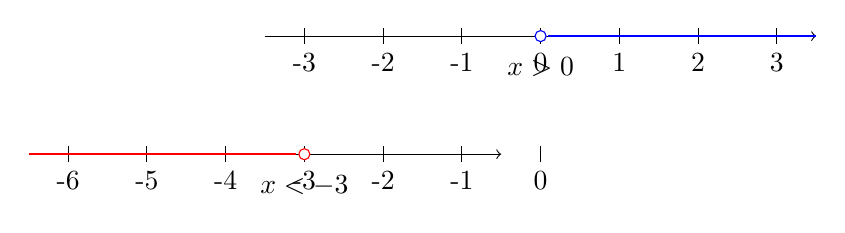
\begin{tikzpicture}
    % Number line for x > 0
    \draw[->] (-3.5,0) -- (3.5,0);
    \foreach \x in {-3,-2,-1,0,1,2,3}
        \draw (\x,0.1) -- (\x,-0.1) node[below] {\x};
    \draw[thick, blue] (0.1,0) -- (3.5,0);
    \draw[blue, fill=white] (0,0) circle(2pt);
    \node at (0,-0.4) {$x > 0$};

    % Number line for x < -3
    \begin{scope}[yshift=-1.5cm]
        \draw[->] (-6.5,0) -- (-0.5,0);
        \foreach \x in {-6,-5,-4,-3,-2,-1,0}
            \draw (\x,0.1) -- (\x,-0.1) node[below] {\x};
        \draw[thick, red] (-6.5,0) -- (-3.1,0);
        \draw[red, fill=white] (-3,0) circle(2pt);
        \node at (-3,-0.4) {$x < -3$};
    \end{scope}
\end{tikzpicture}
} {}{NOTAGS} 
 
 
 
 \ex
{\code{AxNLx25x01x04x006}}{10}
{
\textbf{Represent the following sets on the real line.}

\begin{multicols}{2}
\begin{enumerate}
\item $x \ge -1.5$
\item $x \le \tfrac{2}{3}$
\end{enumerate}
\end{multicols}
} {

 

\[
\text{For } x \ge -1.5: 
\]

A filled circle at $-1.5$ with shading to the right. 

\[
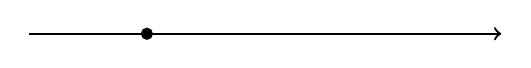
\begin{tikzpicture}
\draw[thick, ->] (-3,0) -- (3,0);
\filldraw [black] (-1.5,0) circle (2pt);
\draw[thick] (-1.5,0) -- (3,0);
\end{tikzpicture}
\]

\[
\text{For } x \le \tfrac{2}{3}:
\]

A filled circle at $\tfrac{2}{3}$ with shading to the left. 

\[
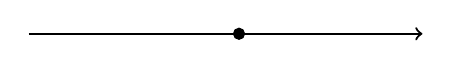
\begin{tikzpicture}
\draw[thick, ->] (-2,0) -- (3,0);
\filldraw [black] (0.67,0) circle (2pt);
\draw[thick] (-2,0) -- (0.67,0);
\end{tikzpicture}
\]
} {}{NOTAGS} 
 
 
 
 \ex
{\code{AxNLx25x01x04x007}}{10}
{
\textbf{Solve the inequality and graph its solution.}

$2x + 7 > 15$
} {

 

\[ 2x + 7 > 15 \]

Subtract 7 from both sides:

\[ 2x > 8 \]

Divide by 2:

\[ x > 4 \]

The solution is all values of \( x \) such that \( x > 4 \).

To graph the solution on a number line:

- Draw a number line.
- Mark an open circle at 4 to show that 4 is not included in the solution.
- Shade the number line to the right of 4 to indicate all numbers greater than 4.

\[
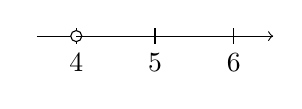
\begin{tikzpicture}
    \draw[->] (3.5,0) -- (6.5,0);
    \foreach \x in {4,5,6}
        \draw (\x,0.1) -- (\x,-0.1) node[below] {\x};
    \node[below] at (3.5,0) {};
    \draw[fill=white] (4,0) circle (2pt);
    \draw (4,0) -- (6.5,0);
\end{tikzpicture}
\]
} {}{NOTAGS} 
 
 
 
 \ex
{\code{AxNLx25x01x04x008}}{10}
{
\textbf{Solve the inequality and graph its solution.}

$5x - 4 < 16$
} {

 

\(5x - 4 < 16\)

Add 4 to both sides:

\[ 
5x < 20 
\]

Divide both sides by 5:

\[ 
x < 4 
\]

The solution in interval notation is \( (-\infty, 4) \).

To graph the solution, draw a number line and shade all values less than 4, using an open circle at 4 to show that it is not included.

\[
\begin{array}{c}
  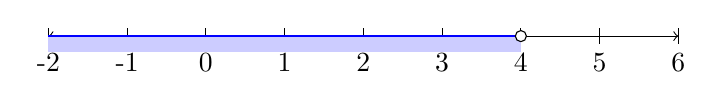
\begin{tikzpicture}
    \draw[<->] (-2,0) -- (6,0);
    \foreach \x in {-2,...,6}
      \draw (\x,0.1) -- (\x,-0.1) node[below] {\x};
    \fill[blue!20] (-2,0) -- (4,0) -- (4,-0.2) -- (-2,-0.2) -- cycle;
    \draw[blue, thick] (-2,0) -- (4,0);
    \draw[fill=white] (4,0) circle (2pt);
  \end{tikzpicture}
\end{array}
\]
} {}{NOTAGS} 
 
 
 
 \ex
{\code{AxNLx25x01x04x009}}{20}
{
\textbf{Solve the inequality and graph its solution.}

$3x - 5 < 12$
} {

 

\( 3x - 5 < 12 \)

Add 5 to both sides:

\( 3x < 17 \)

Divide both sides by 3:

\( x < \frac{17}{3} \)

The solution in interval notation is:

\( x \in \left( -\infty, \frac{17}{3} \right) \)

For the graph:

\[
\begin{array}{c}
\begin{tikzpicture}
    \draw[->] (-1,0) -- (4,0) node[right] {};
    \draw[fill=white] (2.833,0) circle (0.1cm);
    \node at (2.7,-0.5) {\(\frac{17}{3}\)};
    \draw (2.833,0) -- (4,0);
\end{tikzpicture}
\end{array}
\]
} {}{NOTAGS} 
 
 
 
 \ex
{\code{AxNLx25x01x04x010}}{20}
{
\textbf{Solve the inequality and graph its solution.}

$6 - 2x \le 14$
} {

 

\[
6 - 2x \le 14 
\]

Subtract 6 from both sides:

\[
-2x \le 8
\]

Divide both sides by -2, remembering to reverse the inequality sign:

\[
x \ge -4
\]

Thus, the solution to the inequality is:

\[
x \ge -4
\]

The solution graph is on the number line:

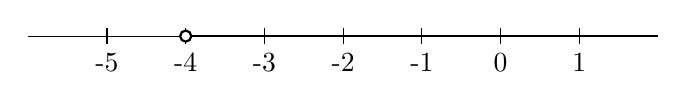
\begin{tikzpicture}
    \draw[-] (-6,0) -- (2,0);
    \foreach \x in {-5,-4,-3,-2,-1,0,1}
        \draw (\x,0.1) -- (\x,-0.1) node[below] {\x};
    \draw[thick] (-4,0) -- (2,0);
    \filldraw[white] (-4,0) circle (2pt);
    \draw[thick] (-4,0) circle (2pt);
\end{tikzpicture}
} {}{NOTAGS} 
 
 
 
 \ex
{\code{AxNLx25x01x04x011}}{20}
{
\textbf{Solve the inequality and graph its solution.}

$-8 - 7x > -1$
} {

 

\(-8 - 7x > -1\)

Add 8 to both sides:

\(-7x > 7\)

Divide both sides by \(-7\), remembering to reverse the inequality sign:

\(x < -1\)

The solution is:

\(x \in (-\infty, -1)\)

The graph of the solution on a number line:
\junk{
\[
\begin{center}
\begin{tikzpicture}
    \draw[-{Stealth[scale=1.5]}] (-3,0) -- (3,0);
    \foreach \x in {-3,-2,-1,0,1,2,3}
        \draw (\x,0.1) -- (\x,-0.1) node[below] {\x};
    \draw[fill=white] (-1,0) circle (3pt);
    \draw[very thick, -] (-3,0) -- (-1,0);
\end{tikzpicture}
\end{center}
\]
}
} {}{NOTAGS} 
 
 
 
 \ex
{\code{AxNLx25x01x04x012}}{20}
{
\textbf{Solve the inequality and graph its solution.}

$-5x + 7 > 12$
} {

 

\(-5x + 7 > 12\)

Subtract 7 from both sides:

\(-5x > 5\)

Divide by \(-5\) and reverse the inequality sign:

\[ x < -1 \]

The solution in interval notation is:

\((- \infty, -1)\)

Graph the solution on a number line:

\[
\begin{array}{c}
\begin{tikzpicture}
\draw[-] (-3,0) -- (2,0);
\draw (0,-0.1) -- (0,0.1) node[below=2pt] {\(-1\)};
\draw[fill=white] (0,0) circle (3pt);
\draw[->] (-3,0) -- (0,0);
\end{tikzpicture}
\end{array}
\]
} {}{NOTAGS} 
 
 
 
 \ex
{\code{AxNLx25x01x04x013}}{20}
{
\textbf{Solve the inequality and graph its solution.}

$6x - 5 < 2x - 13$
} {

 

\begin{align*}
6x - 5 & < 2x - 13 \\ 
6x - 2x & < -13 + 5 \\ 
4x & < -8 \\ 
x & < -2 
\end{align*}

\junk{
\begin{center}
\begin{tikzpicture}
\draw[<->] (-4,0) -- (2,0);
\fill[black] (-2,0) circle (2pt);
\draw (-2,0) node[below] {$-2$};
\node at (-3.5,0.3) {$x$};
\draw (-2,0) to[-open] (2,0);
\end{tikzpicture}
\end{center}
}
} {}{NOTAGS} 
 
 
 
 \ex
{\code{AxNLx25x01x04x014}}{20}
{
\textbf{Solve the inequality and graph its solution.}

$x + 2 \ge 2 + 4x$
} {

 

\begin{align*}
x + 2 &\ge 2 + 4x \\
x + 2 - 2 &\ge 4x + 2 - 2 \\
x &\ge 4x \\
x - 4x &\ge 0 \\
-3x &\ge 0 \\
x &\le 0
\end{align*}

\[
\text{The solution in interval notation is } (-\infty, 0].
\]

\begin{tikzpicture}
\draw[-] (-3,0) -- (3,0);
\draw[fill=black] (0,0) circle (0.1);
\draw[thick] (-3,0) -- (0,0);
\end{tikzpicture}
} {}{NOTAGS} 
 
 
 
 \ex
{\code{AxNLx25x01x04x015}}{20}
{
\textbf{Solve the inequality and graph its solution.}

$4 \ge 2 + x$
} {

 

\begin{align*}
4 &\ge 2 + x \\
4 - 2 &\ge x \\
2 &\ge x \\
x &\le 2 \\
\end{align*}


\[
\text{Solution on a number line:}
\]

\begin{center}
\begin{tikzpicture}
    \draw[->] (-1,0) -- (4,0);
    \foreach \x in {-1, 0, 1, 2, 3, 4}
        \draw (\x,0.1) -- (\x,-0.1) node[below]{\x};
    \draw[fill=black] (2,0) circle (0.1);
    \draw[-] (-1,0) -- (2,0);
\end{tikzpicture}
\end{center}
} {}{NOTAGS} 
 
 
 
 \ex
{\code{AxNLx25x01x04x016}}{20}
{
\textbf{Solve the inequality and graph its solution.}

$\dfrac{x}{5} + 6 < 9$
} {

 

\[
\frac{x}{5} + 6 < 9
\]

Subtract 6 from both sides:

\[
\frac{x}{5} < 3
\]

Multiply both sides by 5:

\[
x < 15
\]

The solution to the inequality is \( x < 15 \).

\[
\begin{tikzpicture}
    \draw[->] (-2,0) -- (5,0); 
    \node at (5.5,0) {};
    \draw[fill=white] (3,0) circle (2pt);
    \draw (3,-0.1) -- (3,0.1);
    \node[below] at (3,0) {15};
    \draw[thick] (-2,0) -- (3,0);
    \node[below right] at (4,0) {$x$};
\end{tikzpicture}
\]
} {}{NOTAGS} 
 
 
 
 \ex
{\code{AxNLx25x01x04x017}}{20}
{
\textbf{Solve the inequality and graph its solution.}

$\dfrac{5x}{2} \ge 15$
} {

 

$x \ge 6$

\begin{center}
\begin{tikzpicture}
    \draw[<->] (4,0) -- (8,0);
    \foreach \x in {4, 5, 6, 7, 8}
        \draw (\x,0.1) -- (\x,-0.1) node[below] {\x};
    \draw[very thick] (6,0) -- (8,0);
    \fill (6,0) circle (2pt);
\end{tikzpicture}
\end{center}
} {}{NOTAGS} 
 
 
 
 \ex
{\code{AxNLx25x01x04x018}}{20}
{
\textbf{Solve the inequality and graph its solution.}

$\dfrac{-4x}{3} \le -16$
} {

 

Solve the inequality:

\[
\frac{-4x}{3} \le -16
\]

Multiply both sides by \(-3\) to eliminate the fraction:

\[
-4x \ge 48
\]

Divide both sides by \(-4\) (remember to reverse the inequality sign):

\[
x \le -12
\]

The solution to the inequality is:

\[
x \le -12
\]

To graph the solution on a number line, plot a closed circle at \(x = -12\) and shade to the left:

\[
\begin{array}{c}
\text{Number line:} \\
\begin{tikzpicture}
    \draw[->] (-15,0) -- (-8,0);
    \foreach \x in {-15,-14,...,-8}
        \draw (\x,0.1) -- (\x,-0.1) node[below] {\x};
    \filldraw (-12,0) circle (2pt) node[above] {};
    \draw[thick] (-15,0) -- (-12,0);
\end{tikzpicture}
\end{array}
\]
} {}{NOTAGS} 
 
 
 
 \ex
{\code{AxNLx25x01x04x019}}{20}
{
\textbf{Solve the inequality and graph its solution.}

$5(x-1) + 3 \ge 5x - 2$
} {

 

\begin{align*}
5(x-1) + 3 &\ge 5x - 2 \\
5x - 5 + 3 &\ge 5x - 2 \\
5x - 2 &\ge 5x - 2 \\
0 &\ge 0
\end{align*}


The inequality holds for all \( x \). Therefore, the solution is all real numbers.

Graphically, this can be represented as a number line with all points shaded:

\[
\begin{tikzpicture}
\draw[thick, -latex] (-4.5,0)--(4.5,0);
\foreach \x in {-4,-3,...,4}
  \draw (\x,0.1)--(\x,-0.1) node[below] {\x};
\draw[thick] (-4,-0.1)--(4,-0.1);
\end{tikzpicture}
\]
} {}{NOTAGS} 
 
 
 
 \ex
{\code{AxNLx25x01x04x020}}{20}
{
\textbf{Solve the inequality and graph its solution.}

$-(x-2) + 4 > 7 - x$
} {

 

$-(x-2) + 4 > 7 - x$

$-x + 2 + 4 > 7 - x$

$-x + 6 > 7 - x$

Add $x$ to both sides:

$6 > 7$

This inequality is false, thus there is no solution. The graph of its solution represents the empty set.
} {}{NOTAGS} 
 
 
 
 \ex
{\code{AxNLx25x01x04x021}}{20}
{
\textbf{Solve the inequality and graph its solution.}

$2(x+1) - 1 \ge 3 - x$
} {

 

\[ 2(x+1) - 1 \ge 3 - x \]

\[ 2x + 2 - 1 \ge 3 - x \]

\[ 2x + 1 \ge 3 - x \]

\[ 2x + x \ge 3 - 1 \]

\[ 3x \ge 2 \]

\[ x \ge \frac{2}{3} \]

Graphically, the solution can be represented on a number line as:

- A solid dot at \( x = \frac{2}{3} \) indicating that the point is included in the solution.
- A ray extending to the right of \( \frac{2}{3} \) showing that all numbers greater than \( \frac{2}{3} \) are solutions.

\begin{tikzpicture}
\draw[<->] (-2,0) -- (2,0);
\fill[black] (0.67,0) circle (2pt);
\draw[thick] (0.67,0) -- (2,0);
\node[below] at (0.67, 0) {\(\frac{2}{3}\)};
\end{tikzpicture}
} {}{NOTAGS} 
 
 
 
 \ex
{\code{AxNLx25x01x04x022}}{20}
{
\textbf{Solve the inequality and graph its solution.}

$6x - 2(x+3) \ge -(4x + 6)$
} {

 

\[ 6x - 2(x+3) \ge -(4x + 6) \]

Start by expanding and simplifying the left side:

\[ 6x - 2x - 6 \ge -(4x + 6) \]

Combine like terms:

\[ 4x - 6 \ge -4x - 6 \]

Add \(4x\) to both sides:

\[ 8x - 6 \ge -6 \]

Add 6 to both sides:

\[ 8x \ge 0 \]

Divide both sides by 8:

\[ x \ge 0 \]

Graph the solution on a number line:

\[
\begin{array}{c}
\bullet \hspace{10pt} \longrightarrow \\
\text{0} 
\end{array}
\]

The filled dot at 0 indicates that 0 is included in the solution \((x \ge 0)\). The arrow points to the right, indicating all numbers greater than 0 are included.
} {}{NOTAGS} 
 
 
 
 \ex
{\code{AxNLx25x01x04x023}}{20}
{
\textbf{Solve the inequality and graph its solution.}

$2 - (x+1) < 5 - 2(x-1)$
} {

 

\begin{align*}
2 - (x+1) &< 5 - 2(x-1) \\
2 - x - 1 &< 5 - 2x + 2 \\
1 - x &< 7 - 2x \\
-x + 2x &< 7 - 1 \\
x &< 6
\end{align*}


The solution to the inequality is \( x < 6 \).

\[
\text{Graph: }
\]

\[
\begin{array}{c}
\begin{tikzpicture}
\draw[<->] (-1,0) -- (7,0);
\foreach \x in {0,1,2,3,4,5,6}
  \draw (\x,0.1) -- (\x,-0.1) node[below] {\x};
\draw[ultra thick,blue,->] (-1,0) -- (5.8,0);
\draw[fill=white] (6,0) circle (0.1);
\end{tikzpicture}
\end{array}
\]
} {}{NOTAGS} 
 
 
 
 \ex
{\code{AxNLx25x01x04x024}}{20}
{
\textbf{Solve the inequality and graph its solution.}

$-2(x-2) + 2(x-2) \le 1$
}
{

 

\[
-2(x-2) + 2(x-2) \le 1
\]

Simplify both sides:

\[
0 \le 1
\]

This inequality holds for all \( x \), so the solution is all real numbers.

The graph of the solution is the entire real number line:

\[
\text{(All real numbers)}
\]
} {}{NOTAGS}




\subsection{Solving Linear Inequalities With Absolute Value \topic{NAL} } 


\subsubsection{With integer solutions \topic{I} } 
 
 
 
 \ex
{\code{AxNALxIx24x12x28x001}}{20}
{Solve the inequality $|3x + 2| > -2$}
{

 

The inequality $|3x + 2| > -2$ is true for all real numbers $x$ because the absolute value expression $|3x + 2|$ is always non-negative, and non-negative numbers are always greater than any negative number, including $-2$. Therefore, the solution is:

$x \in \mathbb{R}$
} {}{NOTAGS}


\ex
{\code{AxNALx25x01x21x007}}{20}
{
Solve these absolute value inequalities:

\begin{multicols}{2}
\begin{enumerate}
\item \(4|3x - 5| < 40\)
\item \(|4x + 1| + 7 \ge 12\)
\end{enumerate}
\end{multicols}
}
{

 

\(4|3x - 5| < 40\)

Divide both sides by 4:

\(|3x - 5| < 10\)

This leads to two inequalities:

\[ 
3x - 5 < 10 \quad \text{and} \quad 3x - 5 > -10 
\]

Solving each:

1. \(3x - 5 < 10\)

   \[
   3x < 15
   \]

   \[
   x < 5
   \]

2. \(3x - 5 > -10\)

   \[
   3x > -5
   \]

   \[
   x > -\frac{5}{3}
   \]

Solution for (1):
\[
-\frac{5}{3} < x < 5
\]

\(|4x + 1| + 7 \ge 12\)

Subtract 7 from both sides:

\(|4x + 1| \ge 5\)

This leads to two inequalities:

\[ 
4x + 1 \ge 5 \quad \text{or} \quad 4x + 1 \le -5 
\]

Solving each:

1. \(4x + 1 \ge 5\)

   \[
   4x \ge 4
   \]

   \[
   x \ge 1
   \]

2. \(4x + 1 \le -5\)

   \[
   4x \le -6
   \]

   \[
   x \le -\frac{3}{2}
   \]

Solution for (2):
\[
x \le -\frac{3}{2} \quad \text{or} \quad x \ge 1
\]
} {}{NOTAGS}



\ex
{\code{AxNALx25x02x05x001}}{25}
{
Solve.

\begin{multicols}{2}
\begin{enumerate}
\item $|x-3|\le 4$

\item $|x+2| \ge 5$


\end{enumerate}
\end{multicols}
}
{

\vspace{4mm}
SOLUTION:

\begin{enumerate}

\item $-4\le x-3\le 4$, which gives $-1\le x\le 7$, so the solution is $[-1,7]$.

\item $x+2\ge 5$ or $x+2\le -5$, which gives $x\ge 3$ or $x\le -7$, so the solution is $(-\infty, -7]\cup [3,\infty)$.

\end{enumerate}

} {}{NOTAGS}





\ex
{\code{AxNALx25x02x05x002}}{25}
{
Solve $|2x+3| > 9$.


}
{

\vspace{4mm}
SOLUTION:

$2x+3>9$ or $2x+3<-9$, which gives $x>3$ or $x<-6$, so the solution is $(-\infty, -6)\cup (3,\infty)$.

} {}{NOTAGS}





\ex
{\code{TESTxxxAxNALx25x03x26x001}}{30}
{
Solve.

\begin{multicols}{2}
\begin{enumerate}
\item $|2x-5|\le 11$

\item $|x+20| \ge 12$


\end{enumerate}
\end{multicols}
}
{
SOLUTION:

For (a)

\(
\begin{array}{rcccl}
-11 & \le & 2x - 5 & \le & 11 \\
-6 & \le & 2x  & \le & 16 \\
-3 & \le & x & \le & 8
\end{array}
\)

\vspace{3mm}
For (b)

Get two inequalities:
Either $x + 20 \le -12$ or $x + 20 \ge 12$.
Solve each to get answer: $x \le -32$ or $x \ge -8$.

} {}{type: TEST}




\ex
{\code{AxNALx25x10x27x001}}{30}
{
Solve.

\begin{multicols}{2}
\begin{enumerate}
\item $|3x-5|\le 13$

\item $|x+10| \ge 2$


\end{enumerate}
\end{multicols}
}
{
SOLUTION: 

For (a)

\(
\begin{array}{rcccl}
-13 & \le & 3x - 5 & \le & 13 \\
-8 & \le & 3x  & \le & 18 \\
\frac{-8}{3} & \le & x & \le & 6
\end{array}
\)

\vspace{3mm}
For (b)

Get two inequalities:
Either $x + 10 \le -2$ or $x + 10 \ge 2$.
Solve each to get answer: $x \le -12$ or $x \ge -8$.


} {}{type: TEST}





\subsection{Linear Equations In Two Variables \topic{TVL} }

\subsubsection{Checking pairs as solutions \topic{C} } 
 
 
 
 \ex
{\code{AxTVLxCx25x01x04x001}}{10}
{
\textbf{For each equation, determine which pairs are solutions.}

$x + y = 3$; pairs: $(1, 2), (-1, 2), (5, -2)$
} {

 

$(1, 2): \quad x + y = 1 + 2 = 3 \quad \text{(solution)}$

$(-1, 2): \quad x + y = -1 + 2 = 1 \quad \text{(not a solution)}$

$(5, -2): \quad x + y = 5 - 2 = 3 \quad \text{(solution)}$
} {}{NOTAGS} 
 
 
 
 \ex
{\code{AxTVLxCx25x01x04x002}}{10}
{
\textbf{For each equation, determine which pairs are solutions.}

$2x + y = -4$; pairs: $(0,0), (-2, 0), (0, -2)$
} {

 

For each pair, substitute into the equation $2x + y = -4$ and determine if it satisfies the equation.

For $(0,0)$:
\[
2(0) + 0 = 0 \neq -4
\]
$(0,0)$ is not a solution.

For $(-2,0)$:
\[
2(-2) + 0 = -4
\]
$(-2,0)$ is a solution.

For $(0,-2)$:
\[
2(0) + (-2) = -2 \neq -4
\]
$(0,-2)$ is not a solution.
} {}{NOTAGS} 
 
 
 
 \ex
{\code{AxTVLxCx25x01x04x003}}{10}
{
\textbf{For each equation, determine which pairs are solutions.}

$2x + y - 1 = 0$; pairs: $(-3, 7), (1, 0), (0, 1)$
}
{

 

$2x + y - 1 = 0$

For $(-3, 7)$:

\[
2(-3) + 7 - 1 = -6 + 7 - 1 = 0
\]

$(-3, 7)$ is a solution.

For $(1, 0)$:

\[
2(1) + 0 - 1 = 2 + 0 - 1 = 1
\]

$(1, 0)$ is not a solution.

For $(0, 1)$:

\[
2(0) + 1 - 1 = 0 + 1 - 1 = 0
\]

$(0, 1)$ is a solution.
} {}{NOTAGS}


\subsubsection{Finding other variable value \topic{OV} } 
 
 
 
 \ex
{\code{AxTVLxOVx25x01x04x004}}{10}
{
\textbf{Find the solution (should be a pair!) which has the given $x$ value.}

\begin{multicols}{2}
$x + y = 3$ ; $x = 2$

$2x + y = -4$ ; $x = \dfrac{1}{2}$
\end{multicols}
} {

 

$x + y = 3$ 

When $x = 2$:

\begin{align*}
2 + y &= 3 \\
y &= 3 - 2 \\
y &= 1
\end{align*}

Solution: $(2, 1)$

\bigskip

$2x + y = -4$

When $x = \dfrac{1}{2}$:

\begin{align*}
2\left(\dfrac{1}{2}\right) + y &= -4 \\
1 + y &= -4 \\
y &= -4 - 1 \\
y &= -5
\end{align*}

Solution: $\left(\dfrac{1}{2}, -5\right)$
} {}{NOTAGS} 
 
 
 
 \ex
{\code{AxTVLxOVx25x01x04x005}}{10}
{
\textbf{Find the solution (should be a pair!) which has the given $x$ value.}

\begin{multicols}{2}
$2x + y - 1 = 0$ ; $x = 2$
\end{multicols}
}
{

 

\begin{align*}
2x + y - 1 &= 0, \quad x = 2 \\
2(2) + y - 1 &= 0 \\
4 + y - 1 &= 0 \\
y + 3 &= 0 \\
y &= -3 \\
\text{Solution: } (x, y) &= (2, -3)
\end{align*}


} {}{NOTAGS}

\subsubsection{Finding solutions \topic{FS} } 
 
 
 
 \ex
{\code{AxTVLxFSx25x01x04x006}}{10}
{
\textbf{Find 3 solutions of each of the following equations.}

\begin{multicols}{2}
$y = 3 x -2$

$2 x + 5 y = 10$
\end{multicols}
} {

 

$y = 3x - 2$

\begin{align*}
\text{If } x = 0, & \quad y = 3(0) - 2 = -2 \quad \Rightarrow (0, -2) \\
\text{If } x = 1, & \quad y = 3(1) - 2 = 1 \quad \Rightarrow (1, 1) \\
\text{If } x = 2, & \quad y = 3(2) - 2 = 4 \quad \Rightarrow (2, 4) \\
\end{align*}

$2x + 5y = 10$

\begin{align*}
\text{If } x = 0, & \quad 2(0) + 5y = 10 \quad \Rightarrow y = 2 \quad \Rightarrow (0, 2) \\
\text{If } y = 0, & \quad 2x + 5(0) = 10 \quad \Rightarrow x = 5 \quad \Rightarrow (5, 0) \\
\text{If } x = 5, & \quad 2(5) + 5y = 10 \quad \Rightarrow 10 + 5y = 10 \quad \Rightarrow y = 0 \quad \Rightarrow (5, 0) \\
\end{align*}

} {}{NOTAGS} 
 
 
 
 \ex
{\code{AxTVLxFSx25x01x04x007}}{10}
{
\textbf{Find 3 solutions of each of the following equations.}

\begin{multicols}{2}
$x + y = 0$

$-2 x + 3 y = 5$
\end{multicols}
} {

 

$x + y = 0$

For the equation $x + y = 0$, we choose various values for $x$:

1. If $x = 1$, then $y = -1$. Thus, the solution is $(1, -1)$.

2. If $x = 2$, then $y = -2$. Thus, the solution is $(2, -2)$.

3. If $x = -3$, then $y = 3$. Thus, the solution is $(-3, 3)$.

$-2x + 3y = 5$

For the equation $-2x + 3y = 5$, we determine $y$ for chosen values of $x$:

1. If $x = 0$, then $-2(0) + 3y = 5 \implies 3y = 5 \implies y = \frac{5}{3}$. Thus, the solution is $\left(0, \frac{5}{3}\right)$.

2. If $x = 1$, then $-2(1) + 3y = 5 \implies -2 + 3y = 5 \implies 3y = 7 \implies y = \frac{7}{3}$. Thus, the solution is $\left(1, \frac{7}{3}\right)$.

3. If $x = -1$, then $-2(-1) + 3y = 5 \implies 2 + 3y = 5 \implies 3y = 3 \implies y = 1$. Thus, the solution is $(-1, 1)$.
} {}{NOTAGS} 
 
 
 
 \ex
{\code{AxTVLxFSx25x01x04x008}}{10}
{
\textbf{Find 3 solutions of each of the following equations.}

\begin{multicols}{2}
$x = 3 y - 4$

$3 x + 4 y = 5$
\end{multicols}
}
{

 

$x = 3y - 4$

\begin{itemize}
    \item Let $y = 0$: \quad $x = 3(0) - 4 = -4$ \quad (Solution: $(x, y) = (-4, 0)$)
    \item Let $y = 1$: \quad $x = 3(1) - 4 = -1$ \quad (Solution: $(x, y) = (-1, 1)$)
    \item Let $y = 2$: \quad $x = 3(2) - 4 = 2$ \quad (Solution: $(x, y) = (2, 2)$)
\end{itemize}

$3x + 4y = 5$

\begin{itemize}
    \item Let $x = 1$: \quad $3(1) + 4y = 5 \Rightarrow 4y = 2 \Rightarrow y = \frac{1}{2}$ \quad (Solution: $(x, y) = \left(1, \frac{1}{2}\right)$)
    \item Let $y = 0$: \quad $3x + 4(0) = 5 \Rightarrow 3x = 5 \Rightarrow x = \frac{5}{3}$ \quad (Solution: $(x, y) = \left(\frac{5}{3}, 0\right)$)
    \item Let $x = 0$: \quad $3(0) + 4y = 5 \Rightarrow 4y = 5 \Rightarrow y = \frac{5}{4}$ \quad (Solution: $(x, y) = \left(0, \frac{5}{4}\right)$)
\end{itemize}
} {}{NOTAGS}


\subsubsection{Graphing Linear Equations \topic{GL} } 
 
 
 
 \ex
{\code{AxTVLxGLx25x01x04x009}}{10}
{
Draw $x$ and $y$ axis on the right. Then plot the points (labeling each point).

$(1, 3)$, $(3, 1)$, $(2, -2)$, $(-3, 4)$, $(-1, -2)$, $(0, 2)$, $(1.5, 0)$, $(0,0)$
} {

 

\[
\begin{tikzpicture}[scale=0.8]
    \draw[<->,thick] (-4,0) -- (4,0) node[anchor=north west]{$x$};
    \draw[<->,thick] (0,-3) -- (0,5) node[anchor=south east]{$y$};

    \foreach \x in {-3,-2,-1,1,2,3} 
        \draw (\x,-0.1) -- (\x,0.1) node[anchor=north]{\x};

    \foreach \y in {-2,-1,1,2,3,4} 
        \draw (-0.1,\y) -- (0.1,\y) node[anchor=east]{\y};

    \node at (1,3) [circle,fill,inner sep=1.5pt,label=above right:{$(1,3)$}]{};
    \node at (3,1) [circle,fill,inner sep=1.5pt,label=above right:{$(3,1)$}]{};
    \node at (2,-2) [circle,fill,inner sep=1.5pt,label=below right:{$(2,-2)$}]{};
    \node at (-3,4) [circle,fill,inner sep=1.5pt,label=above left:{$(-3,4)$}]{};
    \node at (-1,-2) [circle,fill,inner sep=1.5pt,label=below left:{$(-1,-2)$}]{};
    \node at (0,2) [circle,fill,inner sep=1.5pt,label=above right:{$(0,2)$}]{};
    \node at (1.5,0) [circle,fill,inner sep=1.5pt,label=below:{$(1.5,0)$}]{};
    \node at (0,0) [circle,fill,inner sep=1.5pt,label=below left:{$(0,0)$}]{};
\end{tikzpicture}
\]
} {}{NOTAGS} 
 
 
 
 \ex
{\code{AxTVLxGLx25x01x04x010}}{10}
{
For each point: If it is on an axis, state which axis it is on. Otherwise, state which quadrant it is in.

$(-4, 6)$, $(8, 10)$, $(0, 12)$, $(-50, -17)$, $(-100, 0)$, $(0.7, -188.9)$
} {

 

$(-4, 6)$ is in Quadrant II.

$(8, 10)$ is in Quadrant I.

$(0, 12)$ is on the $y$-axis.

$(-50, -17)$ is in Quadrant III.

$(-100, 0)$ is on the $x$-axis.

$(0.7, -188.9)$ is in Quadrant IV.
} {}{NOTAGS} 
 
 
 
 \ex
{\code{AxTVLxGLx25x01x04x011}}{10}
{
On graph paper, graph each equation by plotting some solutions and guessing what the rest looks like.  
Which of the graphs (if any), look like lines?

\begin{multicols}{2}
$x - y = 0$

$y = x^2$
\end{multicols}
} {

 

$x - y = 0 \quad \Rightarrow \quad y = x$

The graph of $y = x$ is a straight line with a slope of 1, passing through the origin.

$y = x^2$

The graph of $y = x^2$ is a parabola opening upwards with its vertex at the origin.

Thus, the graph of $x - y = 0$ looks like a line.
} {}{NOTAGS} 
 
 
 
 \ex
{\code{AxTVLxGLx25x01x04x012}}{10}
{
On graph paper, graph each equation by plotting some solutions and guessing what the rest looks like.  
Which of the graphs (if any), look like lines?

\begin{multicols}{2}
$y + x^2 = 1$

$y = 2x + 1$
\end{multicols}
} {

 

\begin{align*}
y + x^2 &= 1 \\
y &= 1 - x^2
\end{align*}

Plot some solutions:
\begin{itemize}
    \item If $x = 0$, $y = 1 - 0^2 = 1$: point $(0, 1)$.
    \item If $x = 1$, $y = 1 - 1^2 = 0$: point $(1, 0)$.
    \item If $x = -1$, $y = 1 - (-1)^2 = 0$: point $(-1, 0)$.
    \item If $x = 2$, $y = 1 - 2^2 = -3$: point $(2, -3)$.
    \item If $x = -2$, $y = 1 - (-2)^2 = -3$: point $(-2, -3)$.
\end{itemize}
The graph is a parabola opening downwards.

\begin{align*}
y &= 2x + 1
\end{align*}

Plot some solutions:
\begin{itemize}
    \item If $x = 0$, $y = 2 \cdot 0 + 1 = 1$: point $(0, 1)$.
    \item If $x = 1$, $y = 2 \cdot 1 + 1 = 3$: point $(1, 3)$.
    \item If $x = -1$, $y = 2 \cdot (-1) + 1 = -1$: point $(-1, -1)$.
\end{itemize}
The graph is a line.

The equation $y = 2x + 1$ is a line. The equation $y + x^2 = 1$ is not a line.
} {}{NOTAGS} 
 
 
 
 \ex
{\code{AxTVLxGLx25x01x04x013}}{10}
{
\textbf{Graph the set of solutions of each of the following equations (on separate graph paper).}

\begin{multicols}{3}
$y = 3 x - 2$

$2 x + 5 y = 10$
\end{multicols}
} {

 

$y = 3x - 2$

To graph this equation, use the slope-intercept form $y = mx + b$, where $m = 3$ is the slope and $b = -2$ is the y-intercept. Plot the y-intercept $(0, -2)$ and use the slope to find another point: from $(0, -2)$, move up 3 units and right 1 unit to $(1, 1)$. Draw a line through these points.

$2x + 5y = 10$

To graph this, convert to slope-intercept form by solving for $y$:
\[ 5y = -2x + 10 \]
\[ y = -\frac{2}{5}x + 2 \]

Here, the slope $m = -\frac{2}{5}$ and the y-intercept $b = 2$. Plot the y-intercept $(0, 2)$, and use the slope to find another point: from $(0, 2)$, move down 2 units and right 5 units to $(5, 0)$. Draw a line through these points.
} {}{NOTAGS} 
 
 
 
 \ex
{\code{AxTVLxGLx25x01x04x014}}{10}
{
\textbf{Graph the set of solutions of each of the following equations (on separate graph paper).}

\begin{multicols}{3}
$x + y = 0$

$-2 x + 3 y = 5$
\end{multicols}
}
{

 

For graphing each equation separately:

For the equation $x + y = 0$:

1. Rewrite it in slope-intercept form: $y = -x$.
2. Choose points:
   - Let $x = 0$, then $y = 0$. Point: $(0, 0)$.
   - Let $x = 1$, then $y = -1$. Point: $(1, -1)$.
   - Let $x = -1$, then $y = 1$. Point: $(-1, 1)$.
3. Plot the points and draw a straight line through them.

For the equation $-2x + 3y = 5$:

1. Rewrite it in slope-intercept form: $y = \frac{2}{3}x + \frac{5}{3}$.
2. Choose points:
   - Let $x = 0$, then $y = \frac{5}{3}$. Point: $(0, \frac{5}{3})$.
   - Let $y = 0$, then $x = \frac{5}{2}$. Point: $(\frac{5}{2}, 0)$.
3. Plot the points and draw a straight line through them.
} {}{NOTAGS}

\subsection{Polynomial basics \topic{P} } 
 
 
 
 \ex
{\code{AxPx25x01x15x001}}{10}
{
For each expression, is it a polynomial? (Yes or No)

\begin{multicols}{2}
\begin{enumerate}
\item $3x + 5y - 6$
\item $x^2 + x + \dfrac{6}{x}$
\end{enumerate}
\end{multicols}
} {

 

\begin{enumerate}
\item Yes
\item No
\end{enumerate}
} {}{NOTAGS} 
 
 
 
 \ex
{\code{AxPx25x01x15x002}}{10}
{
For each expression, is it a polynomial? (Yes or No)

\begin{multicols}{2}
\begin{enumerate}
\item $x^2 - 5x + 6$
\item $\sqrt{x} + 2x + 6$
\end{enumerate}
\end{multicols}
} {

 

Yes; the expression $x^2 - 5x + 6$ is a polynomial.

No; the expression $\sqrt{x} + 2x + 6$ is not a polynomial.
} {}{NOTAGS} 
 
 
 
 \ex
{\code{AxPx25x01x15x003}}{10}
{
For each expression, is it a polynomial? (Yes or No)

\begin{multicols}{2}
\begin{enumerate}
\item $\left(\dfrac{3}{5}\right)x - 2 + 3x - 1$
\item $\dfrac{3 + x}{2 + x} + 3x - 5$
\end{enumerate}
\end{multicols}
} {

 

1. Yes

2. No
} {}{NOTAGS} 
 
 
 
 \ex
{\code{AxPx25x01x15x004}}{10}
{
Classify the following polynomials as 
(1) monomials, (2) binomials, (3) trinomials, or (4) none of those.

\begin{multicols}{2}
\begin{enumerate}
\item $3x + 5y - 6$
\item $x^2 - 5x + 6$
\end{enumerate}
\end{multicols}
} {

 

(1) $3x + 5y - 6$: Trinomial

(2) $x^2 - 5x + 6$: Trinomial
} {}{NOTAGS} 
 
 
 
 \ex
{\code{AxPx25x01x15x005}}{10}
{
Classify the following polynomials as 
(1) monomials, (2) binomials, (3) trinomials, or (4) none of those.

\begin{multicols}{2}
\begin{enumerate}
\item $5x + 3$
\item $-3x^3y^2z^3$
\end{enumerate}
\end{multicols}
} {

 

$5x + 3$: This is a binomial.

$-3x^3y^2z^3$: This is a monomial.
} {}{NOTAGS} 
 
 
 
 \ex
{\code{AxPx25x01x15x006}}{10}
{
Classify the following polynomials as 
(1) monomials, (2) binomials, (3) trinomials, or (4) none of those.

\begin{multicols}{2}
\begin{enumerate}
\item $3x + 5y$
\item $x^2$
\end{enumerate}
\end{multicols}
} {

 

$3x + 5y$ is a binomial.

$x^2$ is a monomial.
} {}{NOTAGS} 
 
 
 
 \ex
{\code{AxPx25x01x15x007}}{10}
{
Classify the following polynomials as 
(1) monomials, (2) binomials, (3) trinomials, or (4) none of those.

\begin{multicols}{2}
\begin{enumerate}
\item $5x + 3 + 7y - 5xy$
\item $x^3 + 3x - 1$
\end{enumerate}
\end{multicols}
} {

 

$(1)$ $5x + 3 + 7y - 5xy$: None of the above.

$(2)$ $x^3 + 3x - 1$: Trinomial.
} {}{NOTAGS} 
 
 
 
 \ex
{\code{AxPx25x01x15x008}}{10}
{
Circle the terms in each expression, and find the coefficient of each term.

\begin{multicols}{2}
\begin{enumerate}
\item $3x + 5y - 6$
\item $x^2 - 5x + 6$
\end{enumerate}
\end{multicols}
} {

 

$3x + 5y - 6$:

Terms: \(3x\), \(5y\), \(-6\) 

Coefficient of \(3x\): 3 

Coefficient of \(5y\): 5 

Coefficient of \(-6\): \(-6\)

\bigskip

$x^2 - 5x + 6$:

Terms: \(x^2\), \(-5x\), \(6\) 

Coefficient of \(x^2\): 1 

Coefficient of \(-5x\): \(-5\) 

Coefficient of \(6\): 6
} {}{NOTAGS} 
 
 
 
 \ex
{\code{AxPx25x01x15x009}}{10}
{
Circle the terms in each expression, and find the coefficient of each term.

\begin{multicols}{2}
\begin{enumerate}
\item $4x + 4$
\item $-x^2 + x$
\end{enumerate}
\end{multicols}
} {

 

$4x + 4$

Terms: $4x$, $4$

Coefficient of $4x$: 4

Coefficient of 4: 4

\bigskip

$-x^2 + x$

Terms: $-x^2$, $x$

Coefficient of $-x^2$: -1

Coefficient of $x$: 1
} {}{NOTAGS} 
 
 
 
 \ex
{\code{AxPx25x01x15x010}}{10}
{
Circle the terms in each expression, and find the coefficient of each term.

\begin{multicols}{2}
\begin{enumerate}
\item $x + 2y - 1$
\item $x^3$
\end{enumerate}
\end{multicols}
} {

 

1. Terms: \( x \), \( 2y \), \( -1 \)

   Coefficients:

   - \( x \): \( 1 \)
   - \( 2y \): \( 2 \)
   - \( -1 \): \( -1 \)

2. Terms: \( x^3 \)

   Coefficient:

   - \( x^3 \): \( 1 \)
} {}{NOTAGS} 



 \ex
{\code{AxPx25x02x18x001}}{10}
{
Find the leading term and leading coefficient in each polynomial.

\begin{multicols}{2}
\begin{enumerate}
\item $-5x^6 + 4x - 30x^3$
\item $5 - x^7 + 3x - 6x^3$
\end{enumerate}
\end{multicols}
} {

 

1. Leading term: \(-5x^6\), Leading coefficient: \(-5\)

2. Leading term: \(-x^7\), Leading coefficient: \(-1\)
} {}{NOTAGS} 


 \ex
{\code{HWxAxPx25x02x18x002}}{10}
{
Find the leading term and leading coefficient in each polynomial.

\begin{multicols}{2}
\begin{enumerate}
\item $-x^2 - 30 + 2x$
\item $5 + x + x^2 +x^3 +x^4$
\end{enumerate}
\end{multicols}
} {

 

The leading term and leading coefficient in each polynomial are:

1. For $-x^2 - 30 + 2x$: 
   \begin{itemize}
   \item Leading term: $-x^2$
   \item Leading coefficient: $-1$
   \end{itemize}

2. For $5 + x + x^2 + x^3 + x^4$: 
   \begin{itemize}
   \item Leading term: $x^4$
   \item Leading coefficient: $1$
   \end{itemize}
} {}{type: HW} 

 
 
 
 \ex
{\code{AxPx25x01x15x011}}{10}
{
Perform the operation and simplify. Write the answer in descending order of degree.

$(x^2 + 3x - 2) + (3x^2 - 5x - 6)$
} {

 

\[
(x^2 + 3x - 2) + (3x^2 - 5x - 6) = x^2 + 3x^2 + 3x - 5x - 2 - 6
\]

\[
= 4x^2 - 2x - 8
\]
} {}{NOTAGS} 
 
 
 
 \ex
{\code{AxPx25x01x15x012}}{10}
{
Perform the operation and simplify. Write the answer in descending order of degree.

$(3x^3 - 4x - 2x^2) + (3x^2 - 6 + x)$
} {

 

\( (3x^3 - 4x - 2x^2) + (3x^2 - 6 + x) = 3x^3 - 2x^2 + 3x^2 - 4x + x - 6 \)

Combine like terms:

\( = 3x^3 + (3x^2 - 2x^2) + (-4x + x) - 6 \)

\( = 3x^3 + x^2 - 3x - 6 \)
} {}{NOTAGS} 
 
 
 
 \ex
{\code{AxPx25x01x15x013}}{10}
{
Perform the operation and simplify. Write the answer in descending order of degree.

$(5x^3 - 2x - 1) + (3x^5 - 5^2)$
} {

 

\( (5x^3 - 2x - 1) + (3x^5 - 5^2) \)

\( = 3x^5 + 5x^3 - 2x - 1 - 25 \)

\( = 3x^5 + 5x^3 - 2x - 26 \)
} {}{NOTAGS} 
 
 
 
 \ex
{\code{AxPx25x01x15x014}}{10}
{
Perform the operation and simplify. Write the answer in descending order of degree.

$(4x^2y + 3xy - 2) + (3xy - 5xy^2 + 6)$
} {

 

\[
(4x^2y + 3xy - 2) + (3xy - 5xy^2 + 6) = 4x^2y + (3xy + 3xy) - 5xy^2 + (-2 + 6)
\]

\[
= 4x^2y + 6xy - 5xy^2 + 4
\]

\[
= -5xy^2 + 4x^2y + 6xy + 4
\]
} {}{NOTAGS} 
 
 
 
 \ex
{\code{AxPx25x01x15x015}}{10}
{
Perform the operation and simplify. Write the answer in descending order of degree.

$(3x - 4xy - z + x^2) + (-5x^2 + z - 3x)$
} {

 

\( (3x - 4xy - z + x^2) + (-5x^2 + z - 3x) \)

Rearrange and combine like terms:

\[
= x^2 - 5x^2 + 3x - 3x - 4xy - z + z
\]

\[
= -4x^2 - 4xy
\] 

The simplified expression is:

\[ 
-4x^2 - 4xy 
\]
} {}{NOTAGS} 
 
 
 
 \ex
{\code{AxPx25x01x15x016}}{10}
{
Perform the operation and simplify. Write the answer in descending order of degree.

$(x^2 + 3x - 2) + (-3x^2 - 3x + 2)$
} {

 

\((x^2 + 3x - 2) + (-3x^2 - 3x + 2)\)

\[
= x^2 + 3x - 2 - 3x^2 - 3x + 2
\]

\[
= (x^2 - 3x^2) + (3x - 3x) + (-2 + 2)
\]

\[
= -2x^2 + 0x + 0
\]

\[
= -2x^2
\]
} {}{NOTAGS} 
 
 
 
 \ex
{\code{AxPx25x01x15x017}}{10}
{
Perform the operation and simplify. Write the answer in descending order of degree.

$(x^2 + 3x - 2) - (3x^2 - 5x - 6)$
} {\solfig{AxPx25x01x15x017}} {}{NOTAGS} 
 
 
 
 \ex
{\code{AxPx25x01x15x018}}{10}
{
Perform the operation and simplify. Write the answer in descending order of degree.

$(3x^3 - 4x - 2x^2) - (3x^2 - 6 + x)$
} {

 

\( (3x^3 - 4x - 2x^2) - (3x^2 - 6 + x) \)

\( = 3x^3 - 4x - 2x^2 - 3x^2 + 6 - x \)

\( = 3x^3 - 2x^2 - 3x^2 - 4x - x + 6 \)

\( = 3x^3 - 5x^2 - 5x + 6 \)
} {}{NOTAGS} 
 
 
 
 \ex
{\code{AxPx25x01x15x019}}{10}
{
Perform the operation and simplify. Write the answer in descending order of degree.

$(5x^3 - 2x - 1) - (3x^5 - 5^2)$
} {

 

\( (5x^3 - 2x - 1) - (3x^5 - 5^2) = 5x^3 - 2x - 1 - 3x^5 + 25 \)

\( = -3x^5 + 5x^3 - 2x + 24 \)
} {}{NOTAGS} 
 
 
 
 \ex
{\code{AxPx25x01x15x020}}{10}
{
Perform the operation and simplify. Write the answer in descending order of degree.

$(4x^2y + 3xy - 2) - (3xy - 5xy^2 + 6)$
} {

 

\((4x^2y + 3xy - 2) - (3xy - 5xy^2 + 6)\)

\(= 4x^2y + 3xy - 2 - 3xy + 5xy^2 - 6\)

\(= 4x^2y + 5xy^2 + (3xy - 3xy) - 2 - 6\)

\(= 4x^2y + 5xy^2 - 8\)

In descending order of degree:

\(5xy^2 + 4x^2y - 8\)
} {}{NOTAGS} 
 
 
 
 \ex
{\code{AxPx25x01x15x021}}{10}
{
Perform the operation and simplify. Write the answer in descending order of degree.

$(3x - 4xy - z + x^2) - (-5x^2 + z - 3x)$
} {

 

\( (3x - 4xy - z + x^2) - (-5x^2 + z - 3x) \)

\( = 3x - 4xy - z + x^2 + 5x^2 - z + 3x \)

\( = x^2 + 5x^2 + 3x + 3x - z - z - 4xy \)

\( = 6x^2 + 6x - 2z - 4xy \)

Final answer in descending order:

\( 6x^2 - 4xy + 6x - 2z \)
} {}{NOTAGS} 
 
 
 
 \ex
{\code{AxPx25x01x15x022}}{10}
{
Perform the operation and simplify. Write the answer in descending order of degree.

$(x^2 + 3x - 2) - (-3x^2 - 3x + 2)$
} {

 

\( (x^2 + 3x - 2) - (-3x^2 - 3x + 2) = x^2 + 3x - 2 + 3x^2 + 3x - 2 \)

\( = (x^2 + 3x^2) + (3x + 3x) + (-2 - 2) \)

\( = 4x^2 + 6x - 4 \)
} {}{NOTAGS} 
 
 
 
 \ex
{\code{AxPx25x01x15x023}}{10}
{
Evaluate the following (by first simplifying, then evaluating).

$f(x) = 5x^2 + 3x - 5x^2 + x + 1$. Evaluate $f(2)$ and $f(1)$.
} {

 

$f(x) = 5x^2 + 3x - 5x^2 + x + 1$

Simplifying, we have:

$f(x) = (5x^2 - 5x^2) + (3x + x) + 1$

$f(x) = 0 + 4x + 1$

$f(x) = 4x + 1$

Now, evaluate $f(2)$:

$f(2) = 4(2) + 1 = 8 + 1 = 9$

Next, evaluate $f(1)$:

$f(1) = 4(1) + 1 = 4 + 1 = 5$
} {}{NOTAGS} 
 
 
 
 \ex
{\code{AxPx25x01x15x024}}{10}
{
Evaluate the following (by first simplifying, then evaluating).

$f(y) = 8y^3 - 10y - 9 - 7y^3 + 9y + 10$. Evaluate $f(2)$ and $f(1)$.
} {

 

\begin{align*}
f(y) &= 8y^3 - 10y - 9 - 7y^3 + 9y + 10 \\
&= (8y^3 - 7y^3) + (-10y + 9y) + (-9 + 10) \\
&= y^3 - y + 1
\end{align*}

\[
f(2) = 2^3 - 2 + 1 = 8 - 2 + 1 = 7
\]

\[
f(1) = 1^3 - 1 + 1 = 1 - 1 + 1 = 1
\]
} {}{NOTAGS} 
 
 
 
 \ex
{\code{AxPx25x01x15x025}}{20}
{
Evaluate the following (by first simplifying, then evaluating).

$g(t) = -t^2 - t - 1 + t + 2t^2 + 1$. Evaluate $g(-1)$ and $g(0)$.
} {

 

Simplify the expression for \( g(t) \):

\[
g(t) = -t^2 - t - 1 + t + 2t^2 + 1
\]

Combine like terms:

\[
g(t) = (-t^2 + 2t^2) + (-t + t) + (-1 + 1)
\]

\[
g(t) = t^2
\]

Now evaluate \( g(-1) \) and \( g(0) \):

\[
g(-1) = (-1)^2 = 1
\]

\[
g(0) = 0^2 = 0
\]
} {}{NOTAGS} 
 
 
 
 \ex
{\code{AxPx25x01x15x026}}{10}
{
Evaluate the following (by first simplifying, then evaluating).

$h(u) = 3 - 30u^2 + 47u + 15u^2 - 30u + 15u^2 - 17u$. 
Evaluate $h(2024)$ and $g(-3024)$.
}
{

 

First, simplify the expression for \( h(u) \):

\[
h(u) = 3 - 30u^2 + 47u + 15u^2 - 30u + 15u^2 - 17u
\]

Combine like terms:

\[
h(u) = 3 + (-30u^2 + 15u^2 + 15u^2) + (47u - 30u - 17u)
\]

\[
h(u) = 3 + 0u^2 + 0u
\]

\[
h(u) = 3
\]

Now evaluate \( h(2024) \):

\[
h(2024) = 3
\]

There is no \( g(u) \) provided in the exercise, so evaluation of \( g(-3024) \) is not possible based on the given information.
} {}{NOTAGS}



 \ex
{\code{TESTxAxPx25x02x18x001}}{10}
{
Find the leading term and leading coefficient in each polynomial.

\begin{multicols}{2}
\begin{enumerate}
\item $7x^5 - 3x + 2x^3$
\item $5x - x^2 + x^5 - 8x^3$
\end{enumerate}
\end{multicols}
} {

 

The polynomials should be arranged in descending order of the powers of \(x\) to easily identify the leading term.

1. \(7x^5 - 3x + 2x^3\):

   The polynomial in descending order is \(7x^5 + 2x^3 - 3x\).

   Leading term: \(7x^5\)

   Leading coefficient: 7

2. \(5x - x^2 + x^5 - 8x^3\):

   The polynomial in descending order is \(x^5 - 8x^3 - x^2 + 5x\).

   Leading term: \(x^5\)

   Leading coefficient: 1
} {}{NOTAGS} 



\subsection{Polynomial Multiplication \topic{PM} }  
 
 
 
 \ex
{\code{AxPMx25x01x17x001}}{10}
{
Multiply.
\begin{multicols}{2}
\begin{enumerate}
\item $2x(x + 3)=$
\item $-2x(x-2)=$
\end{enumerate}
\end{multicols}
} {

 

\(2x(x + 3) = 2x^2 + 6x\)

\(-2x(x-2) = -2x^2 + 4x\)
} {}{NOTAGS} 
 
 
 
 \ex
{\code{AxPMx25x01x17x002}}{10}
{
Multiply.
\begin{multicols}{2}
\begin{enumerate}
\item $3x^2(x + 5)=$
\item $2x(x^3 - 7x^2 + 4x + 6)=$
\end{enumerate}
\end{multicols}
} {

 

\[ 3x^2(x + 5) = 3x^3 + 15x^2 \]

\[ 2x(x^3 - 7x^2 + 4x + 6) = 2x^4 - 14x^3 + 8x^2 + 12x \]
} {}{NOTAGS} 
 
 
 
 \ex
{\code{AxPMx25x01x17x003}}{10}
{
Multiply.
\begin{multicols}{2}
\begin{enumerate}
\item $-4x^2(-2x^2 - 5x + 6)=$
\item $2xy(x - 2y + xy)=$
\end{enumerate}
\end{multicols}
} {

 

\begin{align*}
1. & \quad -4x^2(-2x^2 - 5x + 6) \\
   & = (-4x^2)(-2x^2) + (-4x^2)(-5x) + (-4x^2)(6) \\
   & = 8x^4 + 20x^3 - 24x^2
\end{align*}

\begin{align*}
2. & \quad 2xy(x - 2y + xy) \\
   & = (2xy)(x) + (2xy)(-2y) + (2xy)(xy) \\
   & = 2x^2y - 4xy^2 + 2x^2y^2
\end{align*}

} {}{NOTAGS} 


 \ex
{\code{AxPMx25x02x12x003}}{10}
{
Multiply.
 $-3x^2(-2x^2 + 3x - 1)=$


} {\solfig{AxPMx25x02x12x003}} {}{NOTAGS} 


 
 
 
 \ex
{\code{AxPMx25x01x17x004}}{10}
{
Multiply.
\begin{multicols}{2}
\begin{enumerate}
\item $(3 - 3x^2 + 6x)\cdot x^2=$
\item $-4xy^2(-2x^2y - 5)=$
\end{enumerate}
\end{multicols}
} {

 

\((3 - 3x^2 + 6x)\cdot x^2 = 3x^2 - 3x^4 + 6x^3\)

\(-4xy^2(-2x^2y - 5) = 8x^3y^3 + 20xy^2\)
} {}{NOTAGS} 
 
 
 
 \ex
{\code{AxPMx25x01x17x005}}{10}
{
Multiply.

$(x+3)(x+2)=$
} {

 

\((x+3)(x+2) = x(x+2) + 3(x+2) = x^2 + 2x + 3x + 6 = x^2 + 5x + 6\)
} {}{NOTAGS} 
 
 
 
 \ex
{\code{AxPMx25x01x17x006}}{10}
{
Multiply.

$(x+5)(x-3)=$
} {

 

\((x+5)(x-3) = x^2 - 3x + 5x - 15 = x^2 + 2x - 15\)
} {}{NOTAGS} 
 
 
 
 \ex
{\code{AxPMx25x01x17x007}}{10}
{
Multiply.

$(2x-3)(5x-6)=$
} {

 

\[
(2x-3)(5x-6) = 2x \cdot 5x + 2x \cdot (-6) + (-3) \cdot 5x + (-3) \cdot (-6)
\]

\[
= 10x^2 - 12x - 15x + 18
\]

\[
= 10x^2 - 27x + 18
\]
} {}{NOTAGS} 

 \ex
{\code{AxPMx25x02x12x001}}{10}
{
Multiply.

$(x-3)(4x-5)=$
} {

SOLUTION: $= 4x^2 - 5x - 12x +15 \ \ \ \ = \ \ \ \ 4x^2 -17x + 15 $
} {}{NOTAGS} 
 
 
 
 \ex
{\code{AxPMx25x01x17x008}}{10}
{
Multiply.

$(x^2 - 5)(-x - 3)=$
} {

 

\((x^2 - 5)(-x - 3) = x^2(-x - 3) - 5(-x - 3)\)

\(= x^2(-x) + x^2(-3) + 5x + 15\)

\(= -x^3 - 3x^2 + 5x + 15\)
} {}{NOTAGS} 
 
 
 
 \ex
{\code{AxPMx25x01x17x009}}{10}
{
Multiply.

$(x+3)(x^2 + 3x + 1)=$
} {

 

\((x+3)(x^2 + 3x + 1) = x(x^2 + 3x + 1) + 3(x^2 + 3x + 1)\)

\(= x^3 + 3x^2 + x + 3x^2 + 9x + 3\)

\(= x^3 + 6x^2 + 10x + 3\)
} {}{NOTAGS} 
 
 
 
 \ex
{\code{AxPMx25x01x17x010}}{10}
{
Multiply.

$(x-3)(x^2 - 6x - 4)=$
} {

 

\((x-3)(x^2 - 6x - 4) = x(x^2 - 6x - 4) - 3(x^2 - 6x - 4)\)

\(= x^3 - 6x^2 - 4x - 3x^2 + 18x + 12\)

\(= x^3 - 9x^2 + 14x + 12\)
} {}{NOTAGS} 
 
 
 
 \ex
{\code{AxPMx25x01x17x011}}{10}
{
Multiply.

$(x^2 + x + 3)(x^2 - 7)=$
} {

 

\((x^2 + x + 3)(x^2 - 7) = x^2(x^2 - 7) + x(x^2 - 7) + 3(x^2 - 7)\)

\[
= x^4 - 7x^2 + x^3 - 7x + 3x^2 - 21
\]

\[
= x^4 + x^3 - 4x^2 - 7x - 21
\]
} {}{NOTAGS} 
 
 
 
 \ex
{\code{AxPMx25x01x17x012}}{10}
{
Multiply.

$(x^2 - 6x - 4)(x - 5)=$
} {

 

\[
(x^2 - 6x - 4)(x - 5) = x^2(x - 5) - 6x(x - 5) - 4(x - 5)
\]

\[
= x^3 - 5x^2 - 6x^2 + 30x - 4x + 20
\]

\[
= x^3 - 11x^2 + 26x + 20
\]
} {}{NOTAGS} 
 
 
 
 \ex
{\code{AxPMx25x01x17x013}}{10}
{
Multiply.

$(x^2 - 2x - 3)(x^2 - x - 4)=$
} {

 

\[
(x^2 - 2x - 3)(x^2 - x - 4) = x^2(x^2 - x - 4) - 2x(x^2 - x - 4) - 3(x^2 - x - 4)
\]

\[
= (x^4 - x^3 - 4x^2) + (-2x^3 + 2x^2 + 8x) + (-3x^2 + 3x + 12)
\]

\[
= x^4 - 3x^3 - 5x^2 + 11x + 12
\]
} {}{NOTAGS} 
 
 
 
 \ex
{\code{AxPMx25x01x17x014}}{10}
{
Multiply.

$(-3x^2 - 2x + 1)(-x^3 - 5x + 6)=$
} {

 

\[
(-3x^2 - 2x + 1)(-x^3 - 5x + 6) = (-3x^2)(-x^3) + (-3x^2)(-5x) + (-3x^2)(6) + (-2x)(-x^3) + (-2x)(-5x) + (-2x)(6) + 1(-x^3) + 1(-5x) + 1(6)
\]

\[
= 3x^5 + 15x^3 - 18x^2 + 2x^4 + 10x^2 - 12x - x^3 - 5x + 6
\]

\[
= 3x^5 + 2x^4 + (15x^3 - x^3) + (-18x^2 + 10x^2) + (-12x - 5x) + 6
\]

\[
= 3x^5 + 2x^4 + 14x^3 - 8x^2 - 17x + 6
\]
} {}{NOTAGS} 
 
 
 
 \ex
{\code{AxPMx25x01x17x015}}{10}
{
Multiply.

$x(x+3)(x+2)=$
} {

 

Expand the given expression:

\[
x(x+3)(x+2) = x[(x+3)(x+2)]
\]

First, expand \((x+3)(x+2)\):

\[
(x+3)(x+2) = x(x+2) + 3(x+2) = x^2 + 2x + 3x + 6 = x^2 + 5x + 6
\]

Now, multiply the result by \(x\):

\[
x(x^2 + 5x + 6) = x^3 + 5x^2 + 6x
\]

Thus, the solution is:

\[
x(x+3)(x+2) = x^3 + 5x^2 + 6x
\]
} {}{NOTAGS} 
 
 
 
 \ex
{\code{AxPMx25x01x17x016}}{10}
{
Multiply.

$(x+1)(x+2)(x+3)=$
} {

 

\begin{align*}
(x+1)(x+2)(x+3) &= ((x+1)(x+2))(x+3) \\
&= (x^2 + 3x + 2)(x+3) \\
&= x^2(x+3) + 3x(x+3) + 2(x+3) \\
&= x^3 + 3x^2 + 3x^2 + 9x + 2x + 6 \\
&= x^3 + 6x^2 + 11x + 6.
\end{align*}

} {}{NOTAGS} 
 
 
 
 \ex
{\code{AxPMx25x01x17x017}}{10}
{
Multiply.

$(x+3)^2=$
} {

 

\((x+3)^2 = (x+3)(x+3)\)

Using the distributive property:

\((x+3)(x+3) = x(x+3) + 3(x+3)\)

Expand:

\(= x^2 + 3x + 3x + 9\)

Combine like terms:

\(= x^2 + 6x + 9\)
} {}{NOTAGS} 
 
 
 
 \ex
{\code{AxPMx25x01x17x018}}{10}
{
Multiply.

$(x-3)^2=$
} {

 

\((x-3)^2 = (x-3)(x-3)\)

\((x-3)^2 = x(x-3) - 3(x-3)\)

\((x-3)^2 = x^2 - 3x - 3x + 9\)

\((x-3)^2 = x^2 - 6x + 9\)
} {}{NOTAGS} 
 
 
 
 \ex
{\code{AxPMx25x01x17x019}}{10}
{
Multiply.

$(x-9)^2=$
} {

 

\((x-9)^2 = (x-9)(x-9)\)

Using the distributive property:

\((x-9)(x-9) = x(x-9) - 9(x-9)\)

\(= x^2 - 9x - 9x + 81\)

Combine like terms:

\(= x^2 - 18x + 81\)
} {}{NOTAGS} 
 
 
 
 \ex
{\code{AxPMx25x01x17x020}}{10}
{
Multiply.

$(x+9)^2=$
} {

 

\((x+9)^2 = (x+9)(x+9)\)

\((x+9)(x+9) = x(x+9) + 9(x+9)\)

\(= x^2 + 9x + 9x + 81\)

\(= x^2 + 18x + 81\)
} {}{NOTAGS} 
 
 
 
 \ex
{\code{AxPMx25x01x17x021}}{10}
{
Multiply.

$(x+1)^2=$
} {

 

\((x+1)^2 = (x+1)(x+1) = x^2 + x + x + 1 = x^2 + 2x + 1\)
} {}{NOTAGS} 
 
 
 
 \ex
{\code{AxPMx25x01x17x022}}{10}
{
Multiply.

$(x-1)^2=$
} {

 

\[(x-1)^2 = (x-1)(x-1) = x^2 - 2x + 1\]
} {}{NOTAGS} 
 
 
 
 \ex
{\code{AxPMx25x01x17x023}}{10}
{
Multiply.

$(x-7)^2=$
} {

 

\((x-7)^2 = (x-7)(x-7)\)

Using the distributive property (FOIL method):

\[
(x-7)(x-7) = x^2 - 7x - 7x + 49
\]

Combine like terms:

\[
x^2 - 14x + 49
\]

Therefore, 

\((x-7)^2 = x^2 - 14x + 49\)
} {}{NOTAGS} 
 
 
 
 \ex
{\code{AxPMx25x01x17x024}}{10}
{
Multiply.

$(x+7)^2=$
} {

 

\((x+7)^2 = (x+7)(x+7)\)

\((x+7)(x+7) = x^2 + 7x + 7x + 49\)

\(= x^2 + 14x + 49\)
} {}{NOTAGS} 
 
 
 
 \ex
{\code{AxPMx25x01x17x025}}{10}
{
Multiply.

$(x-4)(x+4)=$
} {

 

\((x-4)(x+4) = x^2 + 4x - 4x - 16 = x^2 - 16\)
} {}{NOTAGS} 
 
 
 
 \ex
{\code{AxPMx25x01x17x026}}{10}
{
Multiply.

$(x-10)(x+10)=$
} {

 

\[(x-10)(x+10) = x^2 + 10x - 10x - 100 = x^2 - 100\]
} {}{NOTAGS} 
 
 
 
 \ex
{\code{AxPMx25x01x17x027}}{10}
{
Multiply.

$(x+1)(x-1)=$
} {

 

\((x+1)(x-1) = x^2 - 1\)
} {}{NOTAGS} 
 
 
 
 \ex
{\code{AxPMx25x01x17x028}}{10}
{
Multiply.

$(x+3)(x-3)=$
} {

 

\[(x+3)(x-3) = x^2 - 3x + 3x - 9 = x^2 - 9\]
} {}{NOTAGS} 
 
 
 
 \ex
{\code{AxPMx25x01x17x029}}{10}
{
Multiply.

$(a+b)^2=$
} {

 

\((a+b)^2 = a^2 + 2ab + b^2\)
} {}{NOTAGS} 
 
 
 
 \ex
{\code{AxPMx25x01x17x030}}{10}
{
Multiply.

$(a-b)^2=$
} {

 

\((a-b)^2 = (a-b)(a-b) = a(a-b) - b(a-b)\)

\((a-b)^2 = a^2 - ab - ab + b^2\)

\((a-b)^2 = a^2 - 2ab + b^2\)
} {}{NOTAGS} 
 
 
 
 \ex
{\code{AxPMx25x01x17x031}}{10}
{
Multiply.

$(a+b)(a-b)=$
} {

 

\((a+b)(a-b) = a^2 - b^2\)
} {}{NOTAGS} 
 
 
 
 \ex
{\code{AxPMx25x01x18x001}}{10}
{
Expand and simplify.

$5(3x + 4)$
} {

 

\( 5(3x + 4) = 5 \cdot 3x + 5 \cdot 4 = 15x + 20 \)
} {}{NOTAGS} 
 
 
 
 \ex
{\code{AxPMx25x01x18x002}}{10}
{
Expand and simplify.

$x(3x + 4)$
} {

 

\( x(3x + 4) = 3x^2 + 4x \)
} {}{NOTAGS} 
 
 
 
 \ex
{\code{AxPMx25x01x18x003}}{10}
{
Expand and simplify.

$(3x + 4)x$
} {

 

\( (3x + 4)x = 3x^2 + 4x \)
} {}{NOTAGS} 
 
 
 
 \ex
{\code{AxPMx25x01x18x004}}{10}
{
Expand and simplify.

$5x(3x + 4)$
} {

 

\[ 
5x(3x + 4) = 5x \cdot 3x + 5x \cdot 4 
\]

\[ 
= 15x^2 + 20x 
\]
} {}{NOTAGS} 
 
 
 
 \ex
{\code{AxPMx25x01x18x005}}{10}
{
Expand and simplify.

$5x^2(3x + 4)$
} {

 

\( 5x^2(3x + 4) = 5x^2 \cdot 3x + 5x^2 \cdot 4 = 15x^3 + 20x^2 \)
} {}{NOTAGS} 
 
 
 
 \ex
{\code{AxPMx25x01x18x006}}{10}
{
Expand and simplify.

$(3x - 4)(-5x^2)$
} {

 

\[
(3x - 4)(-5x^2) = 3x \cdot (-5x^2) - 4 \cdot (-5x^2)
\]

\[
= -15x^3 + 20x^2
\]
} {}{NOTAGS} 
 
 
 
 \ex
{\code{AxPMx25x01x18x007}}{10}
{
Expand and simplify.

$(3x - 4x^6)(-5x^2)$
} {

 

\((-5x^2)(3x - 4x^6) = (-5x^2)(3x) + (-5x^2)(-4x^6)\)

\((-5x^2)(3x) = -15x^3\)

\((-5x^2)(-4x^6) = 20x^8\)

Therefore, the expanded and simplified expression is:

\(-15x^3 + 20x^8\)
} {}{NOTAGS} 
 
 
 
 \ex
{\code{AxPMx25x01x18x008}}{10}
{
Expand and simplify.

$(3x + 2)(4x + 1)$
} {

 

\( (3x + 2)(4x + 1) = 3x \cdot 4x + 3x \cdot 1 + 2 \cdot 4x + 2 \cdot 1 \)

\( = 12x^2 + 3x + 8x + 2 \)

\( = 12x^2 + 11x + 2 \)
} {}{NOTAGS} 
 
 
 
 \ex
{\code{AxPMx25x01x18x009}}{10}
{
Expand and simplify.

$(3x + 2)(4x + 1)$
} {

 

\((3x + 2)(4x + 1) = 3x \cdot 4x + 3x \cdot 1 + 2 \cdot 4x + 2 \cdot 1\)

\[= 12x^2 + 3x + 8x + 2\]

\[= 12x^2 + 11x + 2\]
} {}{NOTAGS} 
 
 
 
 \ex
{\code{AxPMx25x01x18x010}}{10}
{
Expand and simplify.

$(3x + 2)(4x - 1)$
} {

 

\( (3x + 2)(4x - 1) = 3x \cdot 4x + 3x \cdot (-1) + 2 \cdot 4x + 2 \cdot (-1) \)

\( = 12x^2 - 3x + 8x - 2 \)

\( = 12x^2 + 5x - 2 \)
} {}{NOTAGS} 
 
 
 
 \ex
{\code{AxPMx25x01x18x011}}{10}
{
Expand and simplify.

$(3x - 2)(4x - 1)$
} {

 

\( (3x - 2)(4x - 1) = 3x \cdot 4x + 3x \cdot (-1) - 2 \cdot 4x - 2 \cdot (-1) \)

\( = 12x^2 - 3x - 8x + 2 \)

\( = 12x^2 - 11x + 2 \)
} {}{NOTAGS} 
 
 
 
 \ex
{\code{AxPMx25x01x18x012}}{10}
{
Expand and simplify.

$(3x + 2)^2$
} {

 

\((3x + 2)^2 = (3x + 2)(3x + 2)\)

\(= 3x(3x) + 3x(2) + 2(3x) + 2(2)\)

\(= 9x^2 + 6x + 6x + 4\)

\(= 9x^2 + 12x + 4\)
} {}{NOTAGS} 
 
 
 
 \ex
{\code{AxPMx25x01x18x013}}{10}
{
Expand and simplify.

$(3x - 2)^2$
} {

 

\((3x - 2)^2 = (3x - 2)(3x - 2)\)

\((3x - 2)(3x - 2) = 3x(3x) + 3x(-2) - 2(3x) - 2(-2)\)

\((3x)(3x) = 9x^2\)

\((3x)(-2) = -6x\)

\((-2)(3x) = -6x\)

\((-2)(-2) = 4\)

Combine the terms:

\(9x^2 - 6x - 6x + 4 = 9x^2 - 12x + 4\)
} {}{NOTAGS} 
 
 
 
 \ex
{\code{AxPMx25x01x18x014}}{10}
{
Expand and simplify.

$(3x - 2)(3x + 2)$
} {

 

\((3x - 2)(3x + 2) = (3x)^2 - (2)^2 = 9x^2 - 4\)
} {}{NOTAGS} 
 
 
 
 \ex
{\code{AxPMx25x01x18x015}}{10}
{
Expand and simplify.

$(x - 2)(x + 2)$
} {

 

\((x - 2)(x + 2) = x^2 + 2x - 2x - 4 = x^2 - 4\)
} {}{NOTAGS} 
 
 
 
 \ex
{\code{AxPMx25x01x18x016}}{10}
{
Expand and simplify.

$(3x^2 + 2x + 2)(x + 4)$
} {

 

\( (3x^2 + 2x + 2)(x + 4) = 3x^2(x) + 3x^2(4) + 2x(x) + 2x(4) + 2(x) + 2(4) \)

\( = 3x^3 + 12x^2 + 2x^2 + 8x + 2x + 8 \)

\( = 3x^3 + 14x^2 + 10x + 8 \)
} {}{NOTAGS} 
 
 
 
 \ex
{\code{AxPMx25x01x18x017}}{10}
{
Expand and simplify.

$(3x^2 - 2x + 2)(x - 4)$
}
{

 

\( (3x^2 - 2x + 2)(x - 4) \)

\[
= 3x^2(x) + 3x^2(-4) - 2x(x) - 2x(-4) + 2(x) + 2(-4)
\]

\[
= 3x^3 - 12x^2 - 2x^2 + 8x + 2x - 8
\]

\[
= 3x^3 - 14x^2 + 10x - 8
\]
} {}{NOTAGS}


\subsection{Factoring \topic{F} }

\subsubsection{By Factoring Out GCF \topic{GCF} }  
 
 
  \ex
{\code{AxFxGCFx25x02x12x001}}{10}
{
Factor $20xy^4 - 15y^3 =$

} {

\vspace{5mm}
SOLUTION:
$= 5y^3 (4xy - 3)$
} {}{NOTAGS} 
 
 \ex
{\code{AxFxGCFx25x01x17x001}}{10}
{
Factor out the GCF.
\begin{multicols}{2}
\begin{enumerate}
\item $20A + 30yA =$
\item $30xA - 5A =$
\end{enumerate}
\end{multicols}
} {

 

\begin{enumerate}
    \item $20A + 30yA = A(20 + 30y)$
    \item $30xA - 5A = 5A(6x - 1)$
\end{enumerate}
} {}{NOTAGS} 
 
 
 
 \ex
{\code{AxFxGCFx25x01x17x002}}{10}
{
Factor out the GCF.
\begin{multicols}{2}
\begin{enumerate}
\item $x (x+1) - 5 (x+1) =$
\item $9 (y-1) - 5x (y-1) =$
\end{enumerate}
\end{multicols}
} {

 

\((x+1)(x-5)\)

\((y-1)(9-5x)\)
} {}{NOTAGS} 
 
 
 
 \ex
{\code{AxFxGCFx25x01x17x003}}{10}
{
Factor out the GCF.
\begin{multicols}{2}
\begin{enumerate}
\item $x^2(x^2+4) - 4(x^2+4) =$
\item $x^2(x^2+4) - 4(x^2+4) =$
\end{enumerate}
\end{multicols}
} {

 

\begin{align*}
1. \quad & x^2(x^2+4) - 4(x^2+4) = (x^2 - 4)(x^2 + 4) \\
2. \quad & x^2(x^2+4) - 4(x^2+4) = (x^2 - 4)(x^2 + 4)
\end{align*}

} {}{NOTAGS} 
 
 
 
 \ex
{\code{AxFxGCFx25x01x17x004}}{10}
{
``Shift the negatives''.
\begin{multicols}{2}
\begin{enumerate}
\item $2(-x + 4) = -2(x - 4)$ (example)
\item $3(-y + 7) =$
\end{enumerate}
\end{multicols}
} {

 

$3(-y + 7) = -3(y - 7) = -3y + 21$
} {}{NOTAGS} 
 
 
 
 \ex
{\code{AxFxGCFx25x01x17x005}}{10}
{
``Shift the negatives''.
\begin{multicols}{2}
\begin{enumerate}
\item $-3y(-y + 7) =$
\item $(-x - 5)7 =$
\end{enumerate}
\end{multicols}
} {

 

$-3y(-y + 7) = -3y(-y) + (-3y)(7) = 3y^2 - 21y$

$(-x - 5)7 = (-x)(7) + (-5)(7) = -7x - 35$
} {}{NOTAGS} 
 
 
 
 \ex
{\code{AxFxGCFx25x01x17x006}}{10}
{
``Shift the negatives''.
\begin{multicols}{2}
\begin{enumerate}
\item $(u^2 - 7)(-34y) =$
\item $3x(-y + 7) =$
\end{enumerate}
\end{multicols}
}
{

 

\((-34y)(u^2 - 7) = -34yu^2 + 238y\)

\(3x(-y + 7) = -3xy + 21x\)
} {}{NOTAGS}


\subsubsection{By Grouping \topic{GP} } 
 
 
 
 \ex
{\code{AxFxGPx25x01x17x007}}{15}
{
Factor
$cd + 6c + 4d + 24 =$
} {
\vspace{5mm}
SOLUTION:

$= \hfill c(d + 6) + 4(d + 6) = \hfill (d + 6)(c + 4) \hfill$

} {}{NOTAGS} 
 
 
 
 \ex
{\code{AxFxGPx25x01x17x008}}{10}
{
Factor by Grouping.
$6y^2 + 7y + 24y + 28 =$
} {

 

\[
6y^2 + 7y + 24y + 28 = (6y^2 + 7y) + (24y + 28)
\]

\[
= y(6y + 7) + 4(6y + 7)
\]

\[
= (y + 4)(6y + 7)
\]
} {}{NOTAGS} 
 
 
 
 \ex
{\code{AxFxGPx25x01x17x009}}{10}
{
Factor by Grouping.

$x^2 - x + 4x - 4 =$
} {

 

\begin{align*}
x^2 - x + 4x - 4 &= (x^2 - x) + (4x - 4) \\
&= x(x - 1) + 4(x - 1) \\
&= (x + 4)(x - 1)
\end{align*}

} {}{NOTAGS} 
 
 
 
 \ex
{\code{AxFxGPx25x01x17x010}}{10}
{
Factor by Grouping.

$9p^2 + 12p - 15p - 20 =$
} {

 

\( 9p^2 + 12p - 15p - 20 = \)

Group the terms:

\( (9p^2 + 12p) + (-15p - 20) \)

Factor out the greatest common factor from each group:

\( 3p(3p + 4) - 5(3p + 4) \)

Factor out the common binomial factor:

\( (3p - 5)(3p + 4) \)
} {}{NOTAGS} 
 
 
 
 \ex
{\code{AxFxGPx25x01x17x011}}{10}
{
Factor by Grouping.

$mn - 6m - 4n + 24 =$
} {

 

\( mn - 6m - 4n + 24 = m(n - 6) - 4(n - 6) \)

\( = (m - 4)(n - 6) \)
} {}{NOTAGS} 
 
 
 
 \ex
{\code{AxFxGPx25x01x17x012}}{10}
{
Factor by Grouping.

$x^3 + x^2 + x + 1 =$
} {

 

\[
x^3 + x^2 + x + 1 = (x^3 + x^2) + (x + 1)
\]

\[
= x^2(x + 1) + 1(x + 1)
\]

\[
= (x^2 + 1)(x + 1)
\]
} {}{NOTAGS} 
 
 
 
 \ex
{\code{AxFxGPx25x01x17x013}}{10}
{
Factor by Grouping.

$5x^3 - 3x^2 + 5x - 3 =$
} {

 

\begin{align*}
5x^3 - 3x^2 + 5x - 3 &= (5x^3 - 3x^2) + (5x - 3) \\
&= x^2(5x - 3) + 1(5x - 3) \\
&= (x^2 + 1)(5x - 3)
\end{align*}

} {}{NOTAGS} 
 
 
 
 \ex
{\code{AxFxGPx25x01x17x014}}{10}
{
Factor by Grouping.

$3x^2 - x + 6xy - 2y =$
}
{

 

\[
3x^2 - x + 6xy - 2y = (3x^2 - x) + (6xy - 2y)
\]

\[
= x(3x - 1) + 2y(3x - 1)
\]

\[
= (x + 2y)(3x - 1)
\]
} {}{NOTAGS}

\subsubsection{By Difference Of Squares \topic{DS} }  
 
 
 
 \ex
{\code{AxFxDSx25x01x17x015}}{10}
{
Factor using the GCF and/or using difference of squares.

$x^2 + 9x =$
} {

 

$x^2 + 9x = x(x + 9)$
} {}{NOTAGS} 
 
 
 
 \ex
{\code{AxFxDSx25x01x17x016}}{10}
{
Factor using the GCF and/or using difference of squares.

$x^2 - 9 =$
} {

 

\(x^2 - 9 = (x - 3)(x + 3)\)
} {}{NOTAGS} 
 
 
 
 \ex
{\code{AxFxDSx25x01x17x017}}{10}
{
Factor using the GCF and/or using difference of squares.

$x^2 - 36 =$
} {

 

$x^2 - 36 = (x - 6)(x + 6)$
} {}{NOTAGS} 
 
 
 
 \ex
{\code{AxFxDSx25x01x17x018}}{10}
{
Factor using the GCF and/or using difference of squares.

$15x^4 - 20x^2 =$
} {

 

\[ 
15x^4 - 20x^2 = 5x^2(3x^2 - 4) 
\]
} {}{NOTAGS} 
 
 
 
 \ex
{\code{AxFxDSx25x01x17x019}}{10}
{
Factor using the GCF and/or using difference of squares.

$9x^2 - 1 =$
} {

 

$9x^2 - 1 = (3x)^2 - 1^2 = (3x - 1)(3x + 1)$
} {}{NOTAGS} 
 
 
 
 \ex
{\code{AxFxDSx25x01x17x020}}{10}
{
Factor using the GCF and/or using difference of squares.

$9x^2 - 4y^2 =$
} {

 

\((3x)^2 - (2y)^2 = (3x - 2y)(3x + 2y)\)
} {}{NOTAGS} 
 
 
 
 \ex
{\code{AxFxDSx25x01x17x021}}{10}
{
Factor using the GCF and/or using difference of squares.

$4x^4y^3 - 8x^2y + 4xy =$
} {

 

$4x^4y^3 - 8x^2y + 4xy = 4xy(x^3y^2 - 2x + 1)$
} {}{NOTAGS} 
 
 
 
 \ex
{\code{AxFxDSx25x01x17x022}}{10}
{
Factor using the GCF and/or using difference of squares.

$9 - 25x^2 =$
} {

 

\[ 
9 - 25x^2 = (3)^2 - (5x)^2 
\]

Using the difference of squares formula, \( a^2 - b^2 = (a-b)(a+b) \):

\[ 
9 - 25x^2 = (3 - 5x)(3 + 5x) 
\]
} {}{NOTAGS} 

 \ex
{\code{AxFxDSx25x02x12x001}}{10}
{
Factor.
$25 - 9y^2 =$
} {

\vspace{5mm}
SOLUTION:

$ = \hfill (5)^2 - (3y)^2 = \hfill (5 - 3y)(5 + 3y) \hfill$

} {}{NOTAGS} 
 
 
 
 \ex
{\code{AxFxDSx25x01x17x023}}{10}
{
Factor using the GCF and/or using difference of squares.

$5x^4 - 15x^3 + 25x^2 =$
} {

 

\[
5x^4 - 15x^3 + 25x^2 = 5x^2(x^2 - 3x + 5)
\]
} {}{NOTAGS} 
 
 
 
 \ex
{\code{AxFxDSx25x01x17x024}}{10}
{
Factor using the GCF and/or using difference of squares.

$64x^2 - 49y^2 =$
} {

 

\[
64x^2 - 49y^2 = (8x)^2 - (7y)^2
\]

\[
= (8x - 7y)(8x + 7y)
\]
} {}{NOTAGS} 
 
 
 


\subsubsection{By Trinomials \topic{TRI} } 
 
 
 
 \ex
{\code{AxFxTRIx25x01x17x001}}{10}
{
Factor the trinomial.

$x^2 - 6x + 8 =$
} {

 

$(x - 2)(x - 4)$
} {}{NOTAGS} 
 
 
 
 \ex
{\code{AxFxTRIx25x01x17x002}}{10}
{
Factor the trinomial.

$x^2 + 9x + 18 =$
} {

 

\( x^2 + 9x + 18 = (x + 3)(x + 6) \)
} {}{NOTAGS} 
 
 
 
 \ex
{\code{AxFxTRIx25x01x17x003}}{10}
{
Factor the trinomial.

$x^2 - 5x + 6 =$
} {

 

\((x - 2)(x - 3)\)
} {}{NOTAGS} 
 
 
 
 \ex
{\code{AxFxTRIx25x01x17x004}}{10}
{
Factor the trinomial.

$x^2 - 3x - 10 =$
} {

 

\((x - 5)(x + 2)\)
} {}{NOTAGS} 
 
 
 
 \ex
{\code{AxFxTRIx25x01x17x005}}{10}
{
Factor
$x^2 + 4x - 12 =$
} {

\vspace{5mm}
SOLUTION:

$ = (x - 2)(x + 6) $
} {}{NOTAGS} 
 
 
 
 \ex
{\code{AxFxTRIx25x01x17x006}}{10}
{
Factor the trinomial.

$x^2 - 7x - 8 =$
} {

 

\((x - 8)(x + 1)\)
} {}{NOTAGS} 
 
 
 
 \ex
{\code{AxFxTRIx25x01x17x007}}{10}
{
Factor the trinomial.

$x^2 + 9x + 14 =$
} {

 

\((x + 7)(x + 2)\)
} {}{NOTAGS} 
 
 
 
 \ex
{\code{AxFxTRIx25x01x17x008}}{10}
{
Factor the trinomial.

$x^2 + 9x + 8 =$
} {

 

\((x + 1)(x + 8)\)
} {}{NOTAGS} 
 
 
 
 \ex
{\code{AxFxTRIx25x01x17x009}}{10}
{
Factor the trinomial.

$x^2 - x - 6 =$
} {

 

\((x - 3)(x + 2)\)
} {}{NOTAGS} 
 
 
 
 \ex
{\code{AxFxTRIx25x01x17x010}}{10}
{
Factor the trinomial.

$x^2 + x - 2 =$
} {

 

\[
x^2 + x - 2 = (x + 2)(x - 1)
\]
} {}{NOTAGS} 
 
 
 
 \ex
{\code{AxFxTRIx25x01x17x011}}{10}
{
Factor the trinomial.

$x^2 + 10x + 16 =$
} {

 

\((x + 2)(x + 8)\)
} {}{NOTAGS} 
 
 
 
 \ex
{\code{AxFxTRIx25x01x17x012}}{10}
{
Factor the trinomial.

$x^2 + 15x + 36 =$
} {

 

\((x + 3)(x + 12)\)
} {}{NOTAGS} 
 
 
 
 \ex
{\code{AxFxTRIx25x01x17x013}}{10}
{
Factor the trinomial.

$5x^2 + 21x + 4 =$
} {

 

\((5x^2 + 21x + 4) = (5x + 1)(x + 4)\)
} {}{NOTAGS} 
 
 
 
 \ex
{\code{AxFxTRIx25x01x17x014}}{10}
{
Factor the trinomial.

$8x^2 + 25x + 3 =$
} {

 

\( 8x^2 + 25x + 3 = (8x + 1)(x + 3) \)
} {}{NOTAGS} 
 
 
 
 \ex
{\code{AxFxTRIx25x01x17x015}}{10}
{
Factor the trinomial.

$6x^2 + x - 15 =$
} {

 

\((6x^2 + x - 15) = (3x - 5)(2x + 3)\)
} {}{NOTAGS} 
 
 
 
 \ex
{\code{AxFxTRIx25x01x17x016}}{10}
{
Factor the trinomial.

$2x^2 - 27x - 45 =$
} {

 

\[
2x^2 - 27x - 45 = (2x + 3)(x - 15)
\]
} {}{NOTAGS} 
 
 
 
 \ex
{\code{AxFxTRIx25x01x17x017}}{10}
{
Factor the trinomial.

$5x^2 - 9x + 4 =$
} {

 

\((5x^2 - 9x + 4)\)

First, identify two numbers that multiply to \(5 \times 4 = 20\) and add to \(-9\). These numbers are \(-5\) and \(-4\).

Rewrite the middle term using these numbers: 

\[5x^2 - 5x - 4x + 4\]

Group the terms:

\[(5x^2 - 5x) + (-4x + 4)\]

Factor each group:

\[5x(x - 1) - 4(x - 1)\]

Factor out the common factor \((x - 1)\):

\((5x - 4)(x - 1)\)

Thus, the factored form is:

\((5x - 4)(x - 1)\)
} {}{NOTAGS} 
 
 
 
 \ex
{\code{AxFxTRIx25x01x17x018}}{10}
{
Factor the trinomial.

$4x^2 + 16x + 15 =$
} {

 

\( 4x^2 + 16x + 15 = (2x + 3)(2x + 5) \)
} {}{NOTAGS} 
 
 
 
 \ex
{\code{AxFxTRIx25x01x17x019}}{10}
{
Factor the trinomial.

$9x^2 + 6x + 1 =$
} {

 

\((3x + 1)^2\)
} {}{NOTAGS} 
 
 
 
 \ex
{\code{AxFxTRIx25x01x17x020}}{10}
{
Factor the trinomial.

$9 + 30x + 25x^2 =$
}
{

 

\[ 
9 + 30x + 25x^2 = (3 + 5x)^2 
\]
} {}{NOTAGS}


 \ex
{\code{GROUPxAxFxTRIx25x02x10x001}}{80}
{ 

\begin{enumerate}

\item
	Choose 3 products of the form $(x  + E)(x + F)$, where $E$ and $F$ are numbers  (some of your choices for $E$ and $F$ should include negative numbers).
	
\item	  
	For each choice, multiply it out to get an expression of the form $x^2+Sx +P$, where $S$ and $P$ are numbers.
	
\item	  
	Based on your 3 examples, how do $S$ and $P$ relate to $E$ and $F$?
	
\end{enumerate}	
	 
}
{

 

\begin{enumerate}

\item Example choices:

\begin{itemize}
    \item $(x + 3)(x + 5)$
    \item $(x - 2)(x + 4)$
    \item $(x - 1)(x - 6)$
\end{itemize}

\item Multiplying each:

\begin{align*}
(x + 3)(x + 5) &= x^2 + 5x + 3x + 15 = x^2 + 8x + 15 \\
(x - 2)(x + 4) &= x^2 + 4x - 2x - 8 = x^2 + 2x - 8 \\
(x - 1)(x - 6) &= x^2 - 6x - 1x + 6 = x^2 - 7x + 6
\end{align*}

\item Relationship between $S$, $P$ and $E$, $F$:

For $(x + E)(x + F) = x^2 + Sx + P$, we observe:

\begin{itemize}
    \item $S = E + F$
    \item $P = E \cdot F$
\end{itemize}

\end{enumerate}
} {}{NOTAGS}


\subsubsection{By Some Method \topic{ANY} } 
 
 
 
 \ex
{\code{AxFxANYx25x01x17x001}}{10}
{ Factor.
$x^5 + 4x^3 =$
} {

 

\( x^5 + 4x^3 = x^3(x^2 + 4) \)
} {}{NOTAGS} 
 
 
 
 \ex
{\code{AxFxANYx25x01x17x002}}{10}
{ Factor.
$75m^3 + 12m =$
} {

 

\( 75m^3 + 12m = 3m(25m^2 + 4) \)
} {}{NOTAGS} 
 
 
 
 \ex
{\code{AxFxANYx25x01x17x003}}{10}
{ Factor.
$y^2 - 25 =$
} {

 

\((y^2 - 25) = (y - 5)(y + 5)\)
} {}{NOTAGS} 
 
 
 
 \ex
{\code{AxFxANYx25x01x17x004}}{10}
{ Factor.
$25 - y^2 =$
} {

 

\(25 - y^2 = (5 - y)(5 + y)\)
} {}{NOTAGS} 
 
 
 
 \ex
{\code{AxFxANYx25x01x17x005}}{10}
{ Factor.
$p^2 + 11p + 30 =$
} {

 

\((p + 5)(p + 6)\)
} {}{NOTAGS} 
 
 
 
 \ex
{\code{AxFxANYx25x01x17x006}}{10}
{ Factor.
$a^5 + 9a^3 =$
} {

 

$a^5 + 9a^3 = a^3(a^2 + 9)$
} {}{NOTAGS} 
 
 
 
 \ex
{\code{AxFxANYx25x01x17x007}}{10}
{ Factor.
$a^5 - 9a^3 =$
} {

 

$a^5 - 9a^3 = a^3(a^2 - 9) = a^3(a - 3)(a + 3)$
} {}{NOTAGS} 
 
 
 
 \ex
{\code{AxFxANYx25x01x17x008}}{10}
{ Factor.
$4x^2 + 40x + 84 =$
} {

\vspace{5mm}
SOLUTION:

$= \hfill 4(x^2 + 10x + 21) =  \hfill  4 (x + 3) (x + 7) \hfill $
} {}{NOTAGS} 
 
 
 
 \ex
{\code{AxFxANYx25x01x17x009}}{10}
{ Factor.
$12ab - 6a + 10b - 5 =$
} {

 

\begin{align*}
12ab - 6a + 10b - 5 &= (12ab - 6a) + (10b - 5) \\
&= 6a(2b - 1) + 5(2b - 1) \\
&= (6a + 5)(2b - 1)
\end{align*}

} {}{NOTAGS} 
 
 
 
 \ex
{\code{AxFxANYx25x01x17x010}}{10}
{ Factor.
$y^2 - 5y + 6 =$
} {

 

\( y^2 - 5y + 6 = (y-2)(y-3) \)
} {}{NOTAGS} 
 
 
 
 \ex
{\code{AxFxANYx25x01x17x011}}{10}
{ Factor.
$2n^2 + 13n - 7 =$
} {

 

\((2n - 1)(n + 7)\)
} {}{NOTAGS} 
 
 
 
 \ex
{\code{AxFxANYx25x01x17x012}}{10}
{ Factor.
$4x^5y - 32x^2y =$
} {

 

\( 4x^5y - 32x^2y = 4x^2y(x^3 - 8) = 4x^2y(x - 2)(x^2 + 2x + 4) \)
} {}{NOTAGS} 
 
 
 
 \ex
{\code{AxFxANYx25x01x17x013}}{10}
{ Factor.
$7b^2 + 7b - 42 =$
} {

 

\( 7b^2 + 7b - 42 = 7(b^2 + b - 6) \)

\( b^2 + b - 6 = (b + 3)(b - 2) \)

So, 

\( 7b^2 + 7b - 42 = 7(b + 3)(b - 2) \)
} {}{NOTAGS} 
 
 
 
 \ex
{\code{AxFxANYx25x01x17x014}}{10}
{ Factor.
$36q^2 - 100 =$
} {

 

\begin{align*}
36q^2 - 100 &= (6q)^2 - 10^2 \\
&= (6q - 10)(6q + 10).
\end{align*}

} {}{NOTAGS} 
 
 
 \ex
{\code{AxFxANYx25x02x12x001}}{10}
{ Factor.
$18x^2y - 2y =$
} {

\vspace{5mm}
SOLUTION:

$= 2y(9x^2 - 1) = \hfill 2y( \ (3x)^2  - (1)^2 \ ) =  \hfill 2y (3x - 1) (3x + 1) \hfill $
} {}{NOTAGS}  
 
 
 \ex
{\code{AxFxANYx25x01x17x015}}{15}
{ Factor.
$36x^2y + 15xy - 6y =$
} {

 

\( 36x^2y + 15xy - 6y = 3y(12x^2 + 5x - 2) = 3y(3x - 1)(4x + 2) \)
} {}{NOTAGS} 
 
 
 
 \ex
{\code{AxFxANYx25x01x17x016}}{15}
{ Factor.
$-11 - 10x + x^2 =$
} {

 

\(-11 - 10x + x^2 = (x - 11)(x + 1)\)
} {}{NOTAGS} 
 
 
 
 \ex
{\code{AxFxANYx25x01x17x017}}{15}
{ Factor.
$6n - 7 + n^2 =$
} {

 

$n^2 + 6n - 7 = (n + 7)(n - 1)$
} {}{NOTAGS} 
 
 
 
 \ex
{\code{AxFxANYx25x01x17x018}}{20}
{ Factor.
$8x^2 - 10x - 3 =$
} {

\vspace{5mm}
SOLUTION:

$ = (2x  - 3) (4x + 1)$

} {}{NOTAGS} 
 
 
 
 \ex
{\code{AxFxANYx25x01x17x019}}{15}
{ Factor.
$16x^2 - 24xy + 9y^2 - 64 =$
} {

 

\[
16x^2 - 24xy + 9y^2 - 64 = (4x - 3y)^2 - 8^2 = (4x - 3y - 8)(4x - 3y + 8)
\]
} {}{NOTAGS} 
 
 
 
 \ex
{\code{AxFxANYx25x01x17x020}}{15}
{ Factor.
$9 + 30x + 25x^2 =$
} {

 

\[
9 + 30x + 25x^2 = (3 + 5x)^2
\]
} {}{NOTAGS} 
 
 
 
 \ex
{\code{AxFxANYx25x01x17x021}}{15}
{ Factor.
$49b^2 - 112b + 64 =$
} {

 

\[
49b^2 - 112b + 64 = (7b - 8)^2
\]
} {}{NOTAGS} 
 
 
 
 \ex
{\code{AxFxANYx25x01x17x022}}{10}
{ Factor.
$75x^3 + 12x =$
} {

 

\[ 
75x^3 + 12x = 3x(25x^2 + 4) 
\]
} {}{NOTAGS} 
 
 
 
 \ex
{\code{AxFxANYx25x01x17x023}}{10}
{ Factor.
$x^4 - 81 =$
} {

 

\[
x^4 - 81 = (x^2 - 9)(x^2 + 9)
\]

\[
x^4 - 81 = (x^2 - 3^2)(x^2 + 9)
\]

\[
x^4 - 81 = (x-3)(x+3)(x^2 + 9)
\]
} {}{NOTAGS} 
 
 
 
 \ex
{\code{AxFxANYx25x01x17x024}}{15}
{ Factor.
$3x^4 - 48 =$
} {

 

\( 3x^4 - 48 = 3(x^4 - 16) = 3(x^2 - 4)(x^2 + 4) = 3(x-2)(x+2)(x^2+4) \)
} {}{NOTAGS} 
 
 
 
 \ex
{\code{AxFxANYx25x01x17x025}}{15}
{ Factor.
$y^6 - 1 =$
}
{

 

\[ 
y^6 - 1 = (y^3 - 1)(y^3 + 1) 
\]

First, factor \(y^3 - 1\) and \(y^3 + 1\) using the difference of cubes and sum of cubes formulas:

\[
y^3 - 1 = (y - 1)(y^2 + y + 1)
\]

\[
y^3 + 1 = (y + 1)(y^2 - y + 1)
\]

Combine the results:

\[ 
y^6 - 1 = (y - 1)(y^2 + y + 1)(y + 1)(y^2 - y + 1)
\]
} {}{NOTAGS}




 \ex
{\code{AxFxDSx25x01x17x025}}{15}
{
Factor.

$12x^4 y^3 - 18 x^3 y^2 - 6 x^4 y^6 =$
} {

 

\( 12x^4 y^3 - 18x^3 y^2 - 6x^4 y^6 = 6x^3 y^2 (2xy - 3 - x y^4) \)
} {}{NOTAGS} 
 
 
 
 \ex
{\code{AxFxDSx25x01x17x026}}{15}
{
Factor.

$12x^4 y^3 z - 18 x^3 y^2 z^3 - 9 x^4 z^2 =$
}
{

 

\[ 
12x^4 y^3 z - 18 x^3 y^2 z^3 - 9 x^4 z^2 = 3x^3z(4xy^3 - 6y^2z^2 - 3xz) 
\]
} {}{NOTAGS}



 \ex
{\code{TESTxxxAxFxDSx25x04x28x001}}{35}
{
Factor.  

\begin{multicols}{2}
\begin{enumerate}
\item $3x^3y - 21x^2y + 30xy$
\item  $x^3y^2 - x^3y + 4x^3y - 4x^3$
\end{enumerate}
\end{multicols} 


}
{

SOLUTION:

\vspace{3mm}

a) $3x^3y - 21x^2y + 30xy = 3xy (x^2 - 7x + 10) =
3xy (x -5)(x -2 ) $

\vspace{8mm}

b)  $x^3y^2 - x^3y + 4x^3y - 4x^3 = 
x^3 (y^2 - y + 4y - 4) = x^3 (  y(y - 1) + 4(y - 1) ) =
x^3 (y - 1)(y + 4)$

} {}{NOTAGS}



%BREAK
\end{itemize}
\begin{itemize}

\subsection{Polynomial Division (Synthetic Division, etc) \topic{PDIV} }  
 
 \ex
{\code{AxPDIVx25x01x22x003}}{10}
{
Is \((x-1)\) a factor of \(x^5 + 3x^4 - x + 2\)?
}{

 

To determine if \((x-1)\) is a factor of \(x^5 + 3x^4 - x + 2\), we'll use the Factor Theorem. According to the theorem, \((x-a)\) is a factor of a polynomial if and only if the polynomial evaluates to zero at \(x = a\).

We evaluate the polynomial at \(x = 1\):

\[
f(x) = x^5 + 3x^4 - x + 2
\]

\[
f(1) = (1)^5 + 3(1)^4 - (1) + 2
\]

\[
= 1 + 3 - 1 + 2
\]

\[
= 5
\]

Since \(f(1) = 5 \neq 0\), \((x-1)\) is not a factor of \(x^5 + 3x^4 - x + 2\).
}{}{NOTAGS}

 \ex
{\code{AxPDIVx25x02x24x001}}{10}
{
Is \((x + 1)\) a factor of \(x^5 - 2x^4 - x + 2\)?
}{

 

To determine if \((x + 1)\) is a factor of \(x^5 - 2x^4 - x + 2\), we can apply the Factor Theorem. The Factor Theorem states that \(x - c\) is a factor of \(f(x)\) if and only if \(f(c) = 0\).

Let's find \(f(-1)\):

\[
f(x) = x^5 - 2x^4 - x + 2
\]

\[
f(-1) = (-1)^5 - 2(-1)^4 - (-1) + 2
\]

\[
= -1 - 2 + 1 + 2
\]

\[
= 0
\]

Since \(f(-1) = 0\), \((x + 1)\) is indeed a factor of \(x^5 - 2x^4 - x + 2\).
}{}{NOTAGS}


\ex
{\code{AxPDIVx25x01x22x004}}{10}
{
Use long division to find \((4x^2 - 10x + 6) \div (4x + 2)\).
}{

 

\[
\begin{array}{r|l}
  & x - 3 \\
\hline
4x + 2 & 4x^2 - 10x + 6 \\
  & \underline{4x^2 + 2x} \\
  & \phantom{0} -12x + 6 \\
  & \phantom{0} \underline{-12x - 6} \\
  & \phantom{000000}12 \\
\end{array}
\]

The quotient is \(x - 3\) with a remainder of \(12\). Thus, 

\[
\frac{4x^2 - 10x + 6}{4x + 2} = x - 3 + \frac{12}{4x + 2}
\]
}{}{NOTAGS}


\ex
{\code{AxPDIVx25x02x03x001}}{40}
{ Find the quotient and remainder that result from the following division:
$\dfrac{x^3-2x^2-5x+6}{x+2}$ 
}{

 

\[
\begin{array}{r|l}
x+2 & x^3 - 2x^2 - 5x + 6 \\
\hline
    & \phantom{+}x^2 - 4x + 3 \\
    & \underline{x^3 + 2x^2} \\
    & -4x^2 - 5x \\
    & \underline{-4x^2 - 8x} \\
    & \phantom{+}3x + 6 \\
    & \underline{3x + 6} \\
    & \phantom{+}0 \\
\end{array}
\]

Quotient: \( x^2 - 4x + 3 \)

Remainder: \( 0 \)
}{}{NOTAGS}


\ex
{\code{AxPDIVx25x02x03x004}}{40}
{
Divide $\dfrac{x^4-2x^2-5x+6}{x-3}$ using long division. 
Write your answer in the form $N(x) = d(x) q(x) + r(x)$, where
$N$ is the divident, $d$ is the divisor, $q$ is the quotient, and $r$ is the
remainder.



}{

 

\( N(x) = x^4 - 2x^2 - 5x + 6 \)

\( d(x) = x - 3 \)

Divide using long division:

1. Divide the leading term: \(\frac{x^4}{x} = x^3\)
2. Multiply: \(x^3(x - 3) = x^4 - 3x^3\)
3. Subtract: 
   \[
   (x^4 - 2x^2 - 5x + 6) - (x^4 - 3x^3) = 3x^3 - 2x^2 - 5x + 6
   \]
4. Repeat with \(\frac{3x^3}{x} = 3x^2\)
5. Multiply: \(3x^2(x - 3) = 3x^3 - 9x^2\)
6. Subtract: 
   \[
   (3x^3 - 2x^2 - 5x + 6) - (3x^3 - 9x^2) = 7x^2 - 5x + 6
   \]
7. Repeat with \(\frac{7x^2}{x} = 7x\)
8. Multiply: \(7x(x - 3) = 7x^2 - 21x\)
9. Subtract: 
   \[
   (7x^2 - 5x + 6) - (7x^2 - 21x) = 16x + 6
   \]
10. Repeat with \(\frac{16x}{x} = 16\)
11. Multiply: \(16(x - 3) = 16x - 48\)
12. Subtract: 
    \[
    (16x + 6) - (16x - 48) = 54
    \]

So, \( q(x) = x^3 + 3x^2 + 7x + 16 \) and \( r(x) = 54 \).

Thus, the expression is:

\[ N(x) = (x - 3)(x^3 + 3x^2 + 7x + 16) + 54 \]
}{}{NOTAGS}

\ex
{\code{AxPDIVx25x02x03x002}}{40}
{
Divide $\dfrac{3x^4-2x^3-7x^2+x-2}{x^2-2x+3}$ using long division. 
Write your answer in the form $N(x) = d(x) q(x) + r(x)$, where
$N$ is the numerator, $d$ is the denominator, $q$ is the quotient, and $r$ is the
remainder.

}{

 

\[
\begin{array}{r|l}
x^2 - 2x + 3 & 3x^4 - 2x^3 - 7x^2 + x - 2 \\
\hline
 & 3x^2 \\
 & \underline{-(3x^4 - 6x^3 + 9x^2)} \\
\hline
 & 4x^3 - 16x^2 + x \\
 & \underline{-(4x^3 - 8x^2 + 12x)} \\
\hline
 & -8x^2 - 11x - 2 \\
 & \underline{-(-8x^2 + 16x - 24)} \\
\hline
 & 5x + 22 \\
\end{array}
\]

Therefore, the quotient is \(q(x) = 3x^2 + 4x - 8\) and the remainder is \(r(x) = 5x + 22\).

Thus, the expression can be written as:
\[
N(x) = (x^2 - 2x + 3)(3x^2 + 4x - 8) + (5x + 22)
\]
}{}{NOTAGS}

\ex
{\code{AxPDIVx25x02x03x003}}{40}
{Divide
$\dfrac{x^5+x^4-x^3-x^2+3x-1}{x^2+x+1}$ using long division.
Write your answer in the form $\dfrac{N(x)}{d(x)} = q(x) + \dfrac{r(x)}{d(x)}$,
where $N$ is the numerator, $d$ is the denominator, $q$ is the quotient, and $r$ is the
remainder.

}{

 

\[
\begin{array}{r|l}
x^2 + x + 1 & x^5 + x^4 - x^3 - x^2 + 3x - 1 \\
\hline
 & x^3 + 0x^2 - 2x + 2 \\
\end{array}
\]

First, divide the leading term of the numerator by the leading term of the denominator:

\[
\frac{x^5}{x^2} = x^3
\]

Multiply and subtract:

\[
(x^3)(x^2 + x + 1) = x^5 + x^4 + x^3
\]
\[
x^5 + x^4 - x^3 - (x^5 + x^4 + x^3) = -2x^3 - x^2 + 3x - 1
\]

Next, divide:

\[
\frac{-2x^3}{x^2} = -2x
\]

Multiply and subtract:

\[
(-2x)(x^2 + x + 1) = -2x^3 - 2x^2 - 2x
\]
\[
-2x^3 - x^2 + 3x - 1 - (-2x^3 - 2x^2 - 2x) = x^2 + 5x - 1
\]

Next, divide:

\[
\frac{x^2}{x^2} = 1
\]

Multiply and subtract:

\[
1(x^2 + x + 1) = x^2 + x + 1
\]
\[
x^2 + 5x - 1 - (x^2 + x + 1) = 4x - 2
\]

Result:

\[
\frac{x^5 + x^4 - x^3 - x^2 + 3x - 1}{x^2 + x + 1} = x^3 - 2x + 2 + \frac{4x - 2}{x^2 + x + 1}
\]
}{}{NOTAGS}





\ex
{\code{AxPDIVx25x02x03x006}}{40}
{Find the quotient and remainder that result from the following division:
$\dfrac{x^7-1}{x-1}$
}{

 

When dividing \(x^7 - 1\) by \(x - 1\), we can use polynomial long division or apply the factor theorem. Notice that \(x^7 - 1\) can be rewritten using the formula for the difference of powers:

\[
x^7 - 1 = (x-1)(x^6 + x^5 + x^4 + x^3 + x^2 + x + 1)
\]

Thus, the quotient is:

\[
x^6 + x^5 + x^4 + x^3 + x^2 + x + 1
\]

And the remainder is:

\[
0
\]
}{}{NOTAGS}




\ex
{\code{AxPDIVx25x02x03x008}}{40}
{Find the quotient and remainder that result from the following division:
$\dfrac{-2x^3-7x^2+x-2}{x+1}$

}{

 

\[
\text{Perform polynomial long division on } \dfrac{-2x^3-7x^2+x-2}{x+1}.
\]

1. Divide the first term of the dividend by the first term of the divisor: 
   \[
   \frac{-2x^3}{x} = -2x^2
   \]

2. Multiply the entire divisor by this result and subtract from the dividend:
   \[
   (-2x^3-7x^2+x-2) - (-2x^3 - 2x^2) = -5x^2 + x - 2
   \]

3. Repeat with the new polynomial:
   \[
   \frac{-5x^2}{x} = -5x
   \]

4. Multiply the entire divisor by this result and subtract:
   \[
   (-5x^2 + x - 2) - (-5x^2 - 5x) = 6x - 2
   \]

5. Repeat:
   \[
   \frac{6x}{x} = 6
   \]

6. Multiply and subtract:
   \[
   (6x - 2) - (6x + 6) = -8
   \]

The quotient is \(-2x^2 - 5x + 6\) and the remainder is \(-8\).

Thus, the division yields:
\[
\frac{-2x^3-7x^2+x-2}{x+1} = -2x^2 - 5x + 6 - \frac{8}{x+1}
\]

The quotient is \(-2x^2 - 5x + 6\) and the remainder is \(-8\).
}{}{NOTAGS}

\ex
{\code{AxPDIVx25x02x03x009}}{40}
{Find the quotient and remainder that result from the following division:
$\dfrac{x^4-x^3+x-1}{x-2}$
}{

 

The division of the polynomial can be performed using polynomial long division. The quotient and remainder are:

Quotient: $x^3 + x^2 + 3x + 7$

Remainder: $13$

So, 

\[
\frac{x^4-x^3+x-1}{x-2} = x^3 + x^2 + 3x + 7 + \frac{13}{x-2}
\]
}{}{NOTAGS}

\ex
{\code{AxPDIVx25x02x03x010}}{50}
{
Solve the equation $2x^3-3x^2-11x+6=0$ given that $-2$ is a
zero.
}{

 

Let \( f(x) = 2x^3 - 3x^2 - 11x + 6 \).

Since \(-2\) is a zero, we have:

\[
f(-2) = 2(-2)^3 - 3(-2)^2 - 11(-2) + 6 = 0
\]

To solve the equation, use synthetic division to divide \( f(x) \) by \( x + 2 \).

Write down the coefficients: \( 2, -3, -11, 6 \).

Perform synthetic division:

\[
\begin{array}{r|rrrr}
-2 & 2 & -3 & -11 & 6 \\
   &   & -4 & 14 & -6 \\
\hline
   & 2 & -7 & 3 & 0 \\
\end{array}
\]

The quotient is \( 2x^2 - 7x + 3 \). Now, solve \( 2x^2 - 7x + 3 = 0 \).

To factor \( 2x^2 - 7x + 3 \), find two numbers whose product is \( 2 \times 3 = 6 \) and sum is \(-7\). These numbers are \(-6\) and \(-1\).

Rewrite the middle term:

\[
2x^2 - 6x - x + 3 = 0
\]

Factor by grouping:

\[
2x(x - 3) - 1(x - 3) = 0
\]

Factor out the common factor:

\[
(2x - 1)(x - 3) = 0
\]

Solve for \( x \):

\[
2x - 1 = 0 \quad \Rightarrow \quad x = \frac{1}{2}
\]

\[
x - 3 = 0 \quad \Rightarrow \quad x = 3
\]

Thus, the solutions are \( x = -2, \frac{1}{2}, 3 \).
}{}{NOTAGS}


\ex
{\code{AxPDIVx25x02x03x011}}{50}
{
 Solve the equation $3x^3+7x^2-22x-8=0$ given that $-\frac{1}{3}$ is a
root.
}{

 

Given that \( -\frac{1}{3} \) is a root of the polynomial \( 3x^3 + 7x^2 - 22x - 8 = 0 \), we can use synthetic division or factor theorem to divide the polynomial by \( x + \frac{1}{3} \).

First, multiply the entire polynomial by 3 to clear the fraction:

\[ 3(3x^3 + 7x^2 - 22x - 8) = 9x^3 + 21x^2 - 66x - 24 \]

Now, divide \( 9x^3 + 21x^2 - 66x - 24 \) by \( 3x + 1 \):

\[
\begin{array}{r|rrrr}
  & 9 & 21 & -66 & -24 \\
-\frac{1}{3}\big| &       & 3 & -2 & 20 \\
\hline
  & 9 & 18 & -72 & 0 \\
\end{array}
\]

The quotient is \( 9x^2 + 18x - 72 \).

Factor \( 9x^2 + 18x - 72 \):

\[
9x^2 + 18x - 72 = 9(x^2 + 2x - 8)
\]

We factor further:

\[
x^2 + 2x - 8 = (x + 4)(x - 2)
\]

Thus, the complete factorization of the original polynomial is:

\[
3(3x + 1)(x + 4)(x - 2) = 0
\]

Setting each factor to zero gives the roots:

\[
3x + 1 = 0 \quad \Rightarrow \quad x = -\frac{1}{3}
\]

\[
x + 4 = 0 \quad \Rightarrow \quad x = -4
\]

\[
x - 2 = 0 \quad \Rightarrow \quad x = 2
\]

Therefore, the solutions to the equation are:

\[
x = -\frac{1}{3}, \quad x = -4, \quad x = 2
\]
}{}{NOTAGS}







\ex
{\code{AxPDIVx25x02x03x013}}{10}
{
The remainder from dividing a polynomial $p(x)$ by 
$\left(x-\frac{1}{2}\right)$ is
$\frac{11}{17}$. 
How much is $p\left(\frac{1}{2}\right)$? Which theorem are you using?
}{

\vspace{3mm}
SOLUTION:
The {\bf remainder theorem} states that if a polynomial $f$ is divided by $x-c$ then the remainder 
is $f(c)$. In this case, we know that when we divide $p(x)$ by $(x-\frac{1}{2})$ 
the remainder is $\frac{11}{17}$. Therefore, $p(\frac{1}{2})=\frac{11}{17}$.
}{}{NOTAGS}

\ex
{\code{AxPDIVx25x02x03x113}}{10}
{
The remainder from dividing a polynomial $f(x)$ by 
$\left(x + 5 \right)$ is
$\frac{6}{7}$. 
How much is $f\left( -5 \right)$? Which theorem are you using?
}{

 

$f(-5) = \frac{6}{7}$ \quad (Using the Remainder Theorem)
}{}{NOTAGS}


\ex
{\code{AxPDIVx25x02x03x014}}{10}
{
What is the remainder you would get it you divide the polynomial
$f(x)=x^{103}+x^{50}+2$ by $(x-1)$?
}{

\vspace{3mm}
SOLUTION:
The {\bf remainder theorem} states that if a polynomial $f$ is divided by $x-c$ then the remainder 
is $f(c)$. In this case, if we divide $f(x)=x^{103}+x^{50}+2$ by
$x-1$ (in other words, $c=1$) 
then the remainder will be $f(1)$. But $f(1)$ is very easy to
find: $f(1) = 1^{103}+1^{50}+2 = 1+1+2=4$. Therefore, the remainder is 4.
}{}{NOTAGS}



\ex
{\code{HWxAxPDIVx25x02x03x005}}{40}
{
Divide
$\dfrac{3x^6-2x^3-7x^2-2}{x^2-x+2}$ using long division.
Write your answer in the form $\dfrac{N(x)}{d(x)} = q(x) + \dfrac{r(x)}{d(x)}$,
where $N$ is the divident, $d$ is the divisor, $q$ is the quotient, and $r$ is the
remainder.


}{

 

\[
\begin{array}{c|l}
    x^4 + x^3 + x^2 + x + 1 & x^2-x+2 \\
    \hline
    & 3x^6 - 2x^3 - 7x^2 - 2 \\
    - & (3x^6 - 3x^5 + 6x^4) \\
    \hline
    & 3x^5 - 6x^4 - 2x^3 \\
    - & (3x^5 - 3x^4 + 6x^3) \\
    \hline
    & 3x^4 - 8x^3 - 7x^2 \\
    - & (3x^4 - 3x^3 + 6x^2) \\
    \hline
    & 5x^3 - 13x^2 - 2 \\
    - & (5x^3 - 5x^2 + 10x) \\
    \hline
    & -8x^2 - 10x - 2 \\
    - & (-8x^2 + 8x - 16) \\
    \hline
    & -18x + 14 \\
\end{array}
\]

\[
\frac{3x^6-2x^3-7x^2-2}{x^2-x+2} = x^4 + x^3 + x^2 + x + 1 + \frac{-18x + 14}{x^2-x+2}
\]
}{}{type: HW}


 \ex
{\code{TESTxAxPDIVx25x02x24x001}}{20}
{

\begin{enumerate}
\item Is \((x - 2)\) a factor of \(x^3 - 2x - x + 2\)?

\item The remainder from dividing a polynomial $p(x)$ by $(x+4)$ is
$3$. How much is $p(-4)$? Which theorem are you using?
\end{enumerate}


}{
\vspace{3mm}
SOLUTION: 

For (a): By the factor theorem, we can evaluate at 2:
$$(2)^3 - 2(2) - (2) + 2 = 8 - 4 - 2 + 2 = 4 \neq 0,$$
therefore $(x - 2)$ is {\bf not} a factor.

\vspace{2mm}

For (b):
The {\bf remainder theorem} states that if a polynomial $f$ is divided by $x-c$ then the remainder 
is $f(c)$. In this case, we know that when we divide $p(x)$ by $(x+4)$ (which is the 
same as $x-(-4)$) the remainder is $3$. Therefore, $p(-4)=3$.
}{}{NOTAGS}



\ex
{\code{TESTxAxPDIVx25x02x03x007}}{50}
{Find the quotient and remainder that result from the following division:
$\dfrac{x^3-2x^2-5x+6}{x-3}$ 
% Has remainder zero.

}{

 

Perform polynomial long division on the given division:

Dividend: \(x^3 - 2x^2 - 5x + 6\)

Divisor: \(x - 3\)

1. Divide the first term of the dividend by the first term of the divisor: 

   \[
   \frac{x^3}{x} = x^2
   \]

2. Multiply the entire divisor by \(x^2\) and subtract from the dividend:

   \[
   (x^3 - 2x^2 - 5x + 6) - (x^3 - 3x^2) = x^2 - 5x + 6
   \]

3. Divide the first term of the new dividend by the first term of the divisor:

   \[
   \frac{x^2}{x} = x
   \]

4. Multiply the entire divisor by \(x\) and subtract:

   \[
   (x^2 - 5x + 6) - (x^2 - 3x) = -2x + 6
   \]

5. Divide the first term of the new dividend by the first term of the divisor:

   \[
   \frac{-2x}{x} = -2
   \]

6. Multiply the entire divisor by \(-2\) and subtract:

   \[
   (-2x + 6) - (-2x + 6) = 0
   \]

Since the remainder is zero, the quotient is:

\[
x^2 + x - 2
\]

Thus, the quotient is \(x^2 + x - 2\) and the remainder is \(0\).
}{}{NOTAGS}

\ex
{\code{TESTxAxPDIVx25x03x28x001}}{50}
{Find the quotient and remainder that result from the following division:
$\dfrac{4x^3 + x^2 - 10x + 20}{x+2}$ 
% Has remainder NOT zero.

}{

\solfig{TESTxAxPDIVx25x03x28x001}

}{}{NOTAGS}


\ex
{\code{TESTxxxAxPDIVx25x03x27x001}}{55}
{
Solve the equation $x^3 - 7x^2 + 7x + 15 = 0$ given that $3$ is a
zero.
}{

\solfig{TESTxxxAxPDIVx25x03x27x001}

}{}{NOTAGS}




\subsection{Solving Polynomial Equations \topic{SP} }

\subsubsection{Already Factored \topic{FA} } 
 
 
 
 \ex
{\code{AxSPxFAx01x17x001}}{10}
{
Solve.
\begin{multicols}{2}
\begin{enumerate}
\item $(x+2)(x+3) = 0$
\item $(x-2)(x-3) = 0$
\end{enumerate}
\end{multicols}
} {

 

\begin{enumerate}
\item $(x+2)(x+3) = 0$

Setting each factor to zero, we have:

\[ x+2 = 0 \quad \Rightarrow \quad x = -2 \]

\[ x+3 = 0 \quad \Rightarrow \quad x = -3 \]

Thus, the solutions are \( x = -2 \) and \( x = -3 \).

\item $(x-2)(x-3) = 0$

Setting each factor to zero, we have:

\[ x-2 = 0 \quad \Rightarrow \quad x = 2 \]

\[ x-3 = 0 \quad \Rightarrow \quad x = 3 \]

Thus, the solutions are \( x = 2 \) and \( x = 3 \).
\end{enumerate}
} {}{NOTAGS} 
 
 
 
 \ex
{\code{AxSPxFAx01x17x002}}{10}
{
Solve.
\begin{multicols}{2}
\begin{enumerate}
\item $(x+2)(x-3) = 0$
\item $(x - 2)(x+3) = 0$
\end{enumerate}
\end{multicols}
} {

 

\begin{enumerate}
    \item $(x+2)(x-3) = 0$

          For this equation, set each factor equal to zero:

          $x+2 = 0 \implies x = -2$

          $x-3 = 0 \implies x = 3$

          So, the solutions are $x = -2$ and $x = 3$.
          
    \item $(x-2)(x+3) = 0$

          For this equation, set each factor equal to zero:

          $x-2 = 0 \implies x = 2$

          $x+3 = 0 \implies x = -3$

          So, the solutions are $x = 2$ and $x = -3$.
\end{enumerate}
} {}{NOTAGS} 
 
 
 
 \ex
{\code{AxSPxFAx01x17x003}}{10}
{
Solve.
\begin{multicols}{2}
\begin{enumerate}
\item $(x)(x+8) = 0$
\item $(x+2)(x - 10)(x + 31) = 0$
\end{enumerate}
\end{multicols}
} {

 

For $(x)(x+8) = 0$:

The solutions are found by setting each factor equal to zero:

\[ 
x = 0 \quad \text{or} \quad x + 8 = 0 
\]

\[ 
x = 0 \quad \text{or} \quad x = -8 
\]

Thus, the solutions are \(x = 0\) and \(x = -8\).

For $(x+2)(x - 10)(x + 31) = 0$:

The solutions are found by setting each factor equal to zero:

\[ 
x + 2 = 0 \quad \Rightarrow \quad x = -2 
\]

\[ 
x - 10 = 0 \quad \Rightarrow \quad x = 10 
\]

\[ 
x + 31 = 0 \quad \Rightarrow \quad x = -31 
\]

Thus, the solutions are \(x = -2\), \(x = 10\), and \(x = -31\).
} {}{NOTAGS} 
 
 
 
 \ex
{\code{AxSPxFAx01x17x004}}{10}
{
Solve.
\begin{multicols}{2}
\begin{enumerate}
\item $(x+7)(x+7) = 0$
\item $(x+2)(x+2)(4x) = 0$
\end{enumerate}
\end{multicols}
} {

 

\begin{enumerate}
    \item $(x+7)(x+7) = 0$

    Solving $(x+7)^2 = 0$,

    \[
    x+7 = 0
    \]

    \[
    x = -7
    \]

    \item $(x+2)(x+2)(4x) = 0$

    Solving $(x+2)^2(4x) = 0$, we have:

    \[
    x+2 = 0 \quad \text{or} \quad 4x = 0
    \]

    For $x+2 = 0$,

    \[
    x = -2
    \]

    For $4x = 0$,

    \[
    x = 0
    \]

    The solutions are $x = -2, \, x = 0$.
\end{enumerate}
} {}{NOTAGS} 
 
 
 
 \ex
{\code{AxSPxFAx01x17x005}}{10}
{
Solve.
\begin{multicols}{2}
\begin{enumerate}
\item $(x+7)(2x - 1) = 0$
\item $(7x - 21)(2x) = 0$
\end{enumerate}
\end{multicols}
} {

 

\( (x+7)(2x - 1) = 0 \)

For this equation, we set each factor equal to zero:

\[ x + 7 = 0 \]

\[ x = -7 \]

and

\[ 2x - 1 = 0 \]

\[ 2x = 1 \]

\[ x = \frac{1}{2} \]

Thus, the solutions are \( x = -7 \) and \( x = \frac{1}{2} \).

\vspace{10pt}

\( (7x - 21)(2x) = 0 \)

For this equation, we set each factor equal to zero:

\[ 7x - 21 = 0 \]

\[ 7x = 21 \]

\[ x = 3 \]

and

\[ 2x = 0 \]

\[ x = 0 \]

Thus, the solutions are \( x = 3 \) and \( x = 0 \).
} {}{NOTAGS} 
 
 
 
 \ex
{\code{AxSPxFAx01x17x006}}{10}
{
Solve.

$x(x-1)(5x+1)(x-3) = 0$
} {

 

\[ 
x(x-1)(5x+1)(x-3) = 0 
\]

The given expression is a product of factors. For the product to be zero, at least one of these factors must be zero. Therefore, we solve each factor for zero:

1. \(x = 0\)

2. \(x - 1 = 0 \implies x = 1\)

3. \(5x + 1 = 0 \implies 5x = -1 \implies x = -\frac{1}{5}\)

4. \(x - 3 = 0 \implies x = 3\)

Thus, the solutions to the equation are:

\[
x = 0, \quad x = 1, \quad x = -\frac{1}{5}, \quad x = 3
\]
} {}{NOTAGS} 
 
 
 
 \ex
{\code{AxSPxFAx01x17x013}}{10}
{
Solve.

$(x+2)(x-3)(3x - 5) = 0$
}
{

 

\( (x+2)(x-3)(3x - 5) = 0 \)

To solve the equation, set each factor equal to zero:

1. \( x + 2 = 0 \)

   \[
   x = -2
   \]

2. \( x - 3 = 0 \)

   \[
   x = 3
   \]

3. \( 3x - 5 = 0 \)

   \[
   3x = 5 \quad \Rightarrow \quad x = \frac{5}{3}
   \]

Thus, the solutions are \( x = -2 \), \( x = 3 \), and \( x = \frac{5}{3} \).
} {}{NOTAGS}

\subsubsection{Solve by Factoring \topic{F} } 
 
 
 

 
 
 \ex
{\code{AxSPxFx01x17x008}}{10}
{
Solve.

$x^2 + 9x + 18 = 0$
} {

 

\[
x^2 + 9x + 18 = 0
\]

To solve this quadratic equation, we factor the quadratic polynomial:

\[
x^2 + 9x + 18 = (x + 3)(x + 6) = 0
\]

Setting each factor equal to zero gives:

\[
x + 3 = 0 \quad \Rightarrow \quad x = -3
\]

\[
x + 6 = 0 \quad \Rightarrow \quad x = -6
\]

Thus, the solutions are:

\[
x = -3, \quad x = -6
\]
} {}{NOTAGS} 
 
 
 
 \ex
{\code{AxSPxFx01x17x009}}{10}
{
Solve.

$x^2 - 5x + 6 = 0$
} {

 

The quadratic equation is given by:

\[ x^2 - 5x + 6 = 0 \]

To solve this equation, we factor it:

\[ x^2 - 5x + 6 = (x - 2)(x - 3) = 0 \]

Setting each factor to zero gives:

\[ x - 2 = 0 \quad \Rightarrow \quad x = 2 \]

\[ x - 3 = 0 \quad \Rightarrow \quad x = 3 \]

Thus, the solutions are:

\[ x = 2 \quad \text{and} \quad x = 3 \]
} {}{NOTAGS} 
 
 
 
 \ex
{\code{AxSPxFx01x17x010}}{10}
{
Solve.

$x^2 - 10 = 3x$
} {

 

Rearrange the equation:

\[ x^2 - 3x - 10 = 0 \]

Factor the quadratic:

\[ (x - 5)(x + 2) = 0 \]

Set each factor to zero and solve for \(x\):

\[ x - 5 = 0 \quad \Rightarrow \quad x = 5 \]

\[ x + 2 = 0 \quad \Rightarrow \quad x = -2 \]

The solutions are:

\[ x = 5, \, -2 \]
} {}{NOTAGS} 
 
 
 
 \ex
{\code{AxSPxFx01x17x011}}{10}
{
Solve.

$x^2 + 4x = 12$
} {

 

\[
x^2 + 4x = 12
\]

Subtract 12 from both sides:

\[
x^2 + 4x - 12 = 0
\]

This is a quadratic equation of the form \(ax^2 + bx + c = 0\) where \(a = 1\), \(b = 4\), \(c = -12\).

Use the quadratic formula:

\[
x = \frac{-b \pm \sqrt{b^2 - 4ac}}{2a}
\]

Substitute the values of \(a\), \(b\), and \(c\):

\[
x = \frac{-4 \pm \sqrt{4^2 - 4 \cdot 1 \cdot (-12)}}{2 \cdot 1}
\]

Simplify inside the square root:

\[
x = \frac{-4 \pm \sqrt{16 + 48}}{2}
\]

\[
x = \frac{-4 \pm \sqrt{64}}{2}
\]

Since \(\sqrt{64} = 8\), we have:

\[
x = \frac{-4 \pm 8}{2}
\]

Consider the two cases:

1. \(x = \frac{-4 + 8}{2} = \frac{4}{2} = 2\)

2. \(x = \frac{-4 - 8}{2} = \frac{-12}{2} = -6\)

Thus, the solutions are:

\[
x = 2 \quad \text{and} \quad x = -6
\]
} {}{NOTAGS} 
 
 
 
 \ex
{\code{AxSPxFx01x17x012}}{10}
{
Solve.

$x^2 = 7x + 8$
} {

 

To solve the quadratic equation \(x^2 = 7x + 8\), we start by rearranging it into the standard form \(ax^2 + bx + c = 0\):

\[ 
x^2 - 7x - 8 = 0 
\]

We will use the quadratic formula \(x = \frac{-b \pm \sqrt{b^2 - 4ac}}{2a}\), where \(a = 1\), \(b = -7\), and \(c = -8\).

First, calculate the discriminant:

\[
b^2 - 4ac = (-7)^2 - 4(1)(-8) = 49 + 32 = 81
\]

Now, apply the quadratic formula:

\[
x = \frac{-(-7) \pm \sqrt{81}}{2 \cdot 1} = \frac{7 \pm 9}{2}
\]

This gives us two solutions:

1. \(x = \frac{7 + 9}{2} = 8\)

2. \(x = \frac{7 - 9}{2} = -1\)

Thus, the solutions are \(x = 8\) and \(x = -1\).
} {}{NOTAGS} 
 
 
 
 \ex
{\code{AxSPxFx01x17x014}}{10}
{
Solve.

$x^2 = 9$
} {

 

$x^2 = 9$

Taking the square root of both sides, we get:

$x = \pm \sqrt{9}$

Therefore,

$x = \pm 3$

The solutions are $x = 3$ and $x = -3$.
} {}{NOTAGS} 
 
 
 
 \ex
{\code{AxSPxFx01x17x015}}{10}
{
Solve.

$4x^4 - 20x^3 + 24x^2 = 0$
} {

 

\( 4x^4 - 20x^3 + 24x^2 = 0 \)

First, factor out the greatest common factor:

\( 4x^2(x^2 - 5x + 6) = 0 \)

Set each factor equal to zero:

\( 4x^2 = 0 \)

\( x^2 - 5x + 6 = 0 \)

Solving \( 4x^2 = 0 \):

\( x^2 = 0 \)

\( x = 0 \)

Solving \( x^2 - 5x + 6 = 0 \) using the quadratic formula:

Given \( a = 1 \), \( b = -5 \), \( c = 6 \).

\[ x = \frac{-b \pm \sqrt{b^2 - 4ac}}{2a} \]

\[ x = \frac{-(-5) \pm \sqrt{(-5)^2 - 4 \cdot 1 \cdot 6}}{2 \cdot 1} \]

\[ x = \frac{5 \pm \sqrt{25 - 24}}{2} \]

\[ x = \frac{5 \pm 1}{2} \]

Thus, the solutions are:

\( x = \frac{6}{2} = 3 \)

\( x = \frac{4}{2} = 2 \)

The complete solution set is:

\( x = 0, \, 2, \, 3 \)
} {}{NOTAGS} 
 
 
 
 \ex
{\code{AxSPxFx01x17x016}}{15}
{
Solve.

$12x^3 + 12x^2 = 24x$
} {

 

\[ 
12x^3 + 12x^2 = 24x 
\]

First, factor out the common term:

\[ 
12x^3 + 12x^2 - 24x = 0 
\]

\[ 
12x(x^2 + x - 2) = 0 
\]

Factor the quadratic expression:

\[ 
x^2 + x - 2 = (x+2)(x-1) 
\]

Thus:

\[ 
12x(x+2)(x-1) = 0 
\]

The solutions are:

\[ 
x = 0, \quad x = -2, \quad x = 1 
\]
} {}{NOTAGS} 
 
 
 
 \ex
{\code{AxSPxFx01x17x017}}{10}
{
Solve.

$100x^2 = 9$
} {

 

\[ 
100x^2 = 9 
\]

Divide both sides by 100:

\[ 
x^2 = \frac{9}{100} 
\]

Take the square root of both sides:

\[ 
x = \pm \sqrt{\frac{9}{100}} 
\]

Simplify the square root:

\[ 
x = \pm \frac{3}{10} 
\]

Thus, the solutions are:

\[ 
x = \frac{3}{10} \quad \text{or} \quad x = -\frac{3}{10} 
\]
} {}{NOTAGS} 
 
 
 
 \ex
{\code{AxSPxFx01x17x018}}{10}
{
Solve.

$x^2 + 15x + 36 = 0$
} {

 

\[
x^2 + 15x + 36 = 0
\]

To solve the quadratic equation, we can use the quadratic formula:
\[
x = \frac{{-b \pm \sqrt{{b^2 - 4ac}}}}{2a}
\]
where \( a = 1 \), \( b = 15 \), and \( c = 36 \).

First, calculate the discriminant:
\[
b^2 - 4ac = 15^2 - 4 \cdot 1 \cdot 36 = 225 - 144 = 81
\]

Now substitute into the quadratic formula:
\[
x = \frac{{-15 \pm \sqrt{81}}}{2 \cdot 1} = \frac{{-15 \pm 9}}{2}
\]

This gives the solutions:
\[
x = \frac{{-15 + 9}}{2} = \frac{{-6}}{2} = -3
\]

\[
x = \frac{{-15 - 9}}{2} = \frac{{-24}}{2} = -12
\]

Thus, the solutions are:
\[
x = -3 \quad \text{and} \quad x = -12
\]
} {}{NOTAGS} 
 
 
 
 \ex
{\code{AxSPxFx01x17x019}}{10}
{
Solve.

$5x^2 + 21x + 4 = 0$
} {

 

To solve the quadratic equation \(5x^2 + 21x + 4 = 0\), we use the quadratic formula:

\[ x = \frac{-b \pm \sqrt{b^2 - 4ac}}{2a} \]

where \(a = 5\), \(b = 21\), and \(c = 4\).

First, calculate the discriminant:

\[ b^2 - 4ac = 21^2 - 4(5)(4) = 441 - 80 = 361 \]

Since the discriminant \(361\) is a perfect square, the roots are real and distinct. Now compute the roots:

\[ x = \frac{-21 \pm \sqrt{361}}{2 \times 5} \]

\[ x = \frac{-21 \pm 19}{10} \]

This gives us the two solutions:

\[ x_1 = \frac{-21 + 19}{10} = \frac{-2}{10} = -\frac{1}{5} \]

\[ x_2 = \frac{-21 - 19}{10} = \frac{-40}{10} = -4 \]

Thus, the solutions are:

\[ x = -\frac{1}{5} \quad \text{and} \quad x = -4 \]
} {}{NOTAGS} 
 
 
 
 \ex
{\code{AxSPxFx01x17x020}}{15}
{
Solve.

$8x^2 + 80x + 200 = 0$
} {

 

\[
8x^2 + 80x + 200 = 0
\]

First, divide the entire equation by 8:

\[
x^2 + 10x + 25 = 0
\]

This is a perfect square trinomial:

\[
(x + 5)^2 = 0
\]

Solving for \(x\), we take the square root of both sides:

\[
x + 5 = 0
\]

Subtract 5 from both sides:

\[
x = -5
\]

Thus, the solution is:

\[ 
x = -5 
\]
} {}{NOTAGS} 
 
 
 
 \ex
{\code{AxSPxFx01x17x021}}{10}
{
Solve.

$6x^3 = 24x$
} {

 

\[ 
6x^3 = 24x 
\]

First, divide both sides by 6:

\[ 
x^3 = 4x 
\]

Rearrange the equation:

\[ 
x^3 - 4x = 0 
\]

Factor out \(x\):

\[ 
x(x^2 - 4) = 0 
\]

Set each factor to zero:

1. \(x = 0\)

2. \(x^2 - 4 = 0\)

Solve \(x^2 - 4 = 0\):

\[
x^2 = 4 
\]

Taking the square root of both sides:

\[
x = \pm 2 
\]

Thus, the solutions are:

\[
x = 0, \quad x = 2, \quad x = -2 
\]
} {}{NOTAGS} 
 
 
 
 \ex
{\code{AxSPxFx01x17x022}}{20}
{
Solve (only allow real solutions).

$5x^2 + 4 = 9x$
} {

 

\( 5x^2 + 4 = 9x \)

Rearrange the equation:

\( 5x^2 - 9x + 4 = 0 \)

Solve using the quadratic formula \( x = \frac{-b \pm \sqrt{b^2 - 4ac}}{2a} \), where \( a = 5 \), \( b = -9 \), and \( c = 4 \):

\[
x = \frac{-(-9) \pm \sqrt{(-9)^2 - 4 \cdot 5 \cdot 4}}{2 \cdot 5}
\]

\[
x = \frac{9 \pm \sqrt{81 - 80}}{10}
\]

\[
x = \frac{9 \pm \sqrt{1}}{10}
\]

\[
x = \frac{9 \pm 1}{10}
\]

\[
x = \frac{10}{10}, \quad x = \frac{8}{10}
\]

\[
x = 1, \quad x = 0.8
\]

The real solutions are \( x = 1 \) and \( x = 0.8 \).
} {}{NOTAGS} 
 
 
 



\ex
{\code{AxSPxFx25x02x26x001}}{20}
{
Solve (complex solutions allowed): 
 $x^2 + 12 = -7x$

}{

 

Solve \( x^2 + 12 = -7x \):

First, rearrange the equation:

\[
x^2 + 7x + 12 = 0
\]

Use the quadratic formula, \( x = \frac{-b \pm \sqrt{b^2 - 4ac}}{2a} \), where \( a = 1 \), \( b = 7 \), and \( c = 12 \):

\[
x = \frac{-7 \pm \sqrt{7^2 - 4 \cdot 1 \cdot 12}}{2 \cdot 1}
\]

Calculate the discriminant:

\[
b^2 - 4ac = 7^2 - 4 \cdot 1 \cdot 12 = 49 - 48 = 1
\]

Substitute back into the quadratic formula:

\[
x = \frac{-7 \pm \sqrt{1}}{2}
\]

Calculate the roots:

\[
x = \frac{-7 \pm 1}{2}
\]

Two solutions:

\[
x = \frac{-7 + 1}{2} = \frac{-6}{2} = -3
\]

\[
x = \frac{-7 - 1}{2} = \frac{-8}{2} = -4
\]

The solutions are:

\[
x = -3 \quad \text{and} \quad x = -4
\]
}{}{NOTAGS}



 \ex
{\code{TESTxAxSPxFx01x17x007}}{15}
{
Solve.

$x^2 - 6x + 8 = 0$
} {

SOLUTION:

$(x - 2)(x - 4) = 0$ so $x = 2, 4$.

} {}{NOTAGS} 
 

 \ex
{\code{TESTxAxSPxFx25x01x20x023}}{15}
{
 Solve the equation.

$-5x - 2 = -3x^2$ 
}
{

SOLUTION:

$3x^2 - 5x - 2 = 0$ then by factoring: $(3x + 1) (x - 2) = 0$, so $x = -\dfrac{1}{3}, \ \ 2$

} {}{NOTAGS}


 \ex
{\code{TESTxAxSPxFx25x04x28x001}}{25} 
{
 Solve. 
$7x^2 - 8x  = -1$ 
}
{

SOLUTION:

\vspace{3mm}

$
\begin{array}{ccc}
7x^2 - 8x  & = & -1 \\ 
7x^2 - 8x  + 1 & = & 0 \\ 
(7x  - 1)(x - 1) & = & 0 \\ 
x  & = & \frac{1}{7}, 1
\end{array}
$ 

} {}{NOTAGS}


\subsubsection{Solve by Quadratic Equation \topic{QE} } 
 
 
 
 \ex
{\code{AxSPxQEx25x01x20x005}}{40}
{
 Solve each equation  (complex solutions are NOT allowed):
\begin{multicols}{2}
\begin{enumerate}
\item $2x^2 - 2x = 6$
\item $x^2 + x + 2 = 0$
\end{enumerate}
\end{multicols}
} {

 

1. Solve \(2x^2 - 2x = 6\):

\[
2x^2 - 2x - 6 = 0
\]

Divide the entire equation by 2:

\[
x^2 - x - 3 = 0
\]

Factor the quadratic:

\[
(x - 3)(x + 1) = 0
\]

Set each factor to zero:

\[
x - 3 = 0 \quad \text{or} \quad x + 1 = 0
\]

Solutions:

\[
x = 3 \quad \text{or} \quad x = -1
\]

2. Solve \(x^2 + x + 2 = 0\):

Since this equation does not factor nicely, use the quadratic formula:

\[
x = \frac{-b \pm \sqrt{b^2 - 4ac}}{2a} 
\]

For \(a = 1\), \(b = 1\), \(c = 2\):

\[
x = \frac{-1 \pm \sqrt{1^2 - 4 \cdot 1 \cdot 2}}{2 \cdot 1} 
\]

\[
x = \frac{-1 \pm \sqrt{1 - 8}}{2}
\]

\[
x = \frac{-1 \pm \sqrt{-7}}{2}
\]

Since the discriminant is negative, there are no real solutions for \(x\).
} {}{NOTAGS} 
 
 
 
 \ex
{\code{AxSPxQEx25x01x20x027}}{40}
{
 Solve (complex solutions are allowed):
\begin{enumerate}
\item \(x^2 + 9x = -14\)
\item \(y^2 = 2y + 35\)
\end{enumerate}

} {

 

\begin{enumerate}
    \item \(x^2 + 9x = -14\)

    \begin{align*}
    x^2 + 9x + 14 &= 0 \\
    (x+7)(x+2) &= 0 \\
    x+7 &= 0 \quad \text{or} \quad x+2 = 0 \\
    x &= -7 \quad \text{or} \quad x = -2
    \end{align*}

    \item \(y^2 = 2y + 35\)

    \begin{align*}
    y^2 - 2y - 35 &= 0 \\
    (y-7)(y+5) &= 0 \\
    y-7 &= 0 \quad \text{or} \quad y+5 = 0 \\
    y &= 7 \quad \text{or} \quad y = -5
    \end{align*}

\end{enumerate}
} {}{NOTAGS} 
 
 
 
 \ex
{\code{AxSPxQEx25x01x20x030}}{40}
{
Solve.
\begin{enumerate}
\item \(3u^2 - 6u = -2\)
\item \(y^2 = 2y - 2\)
\end{enumerate}
}
{

 

\begin{enumerate}
\item \(3u^2 - 6u = -2\)

\begin{align*}
3u^2 - 6u + 2 &= 0 \\
u &= \frac{-b \pm \sqrt{b^2 - 4ac}}{2a} \\
a &= 3, \quad b = -6, \quad c = 2 \\
u &= \frac{-(-6) \pm \sqrt{(-6)^2 - 4 \cdot 3 \cdot 2}}{2 \cdot 3} \\
u &= \frac{6 \pm \sqrt{36 - 24}}{6} \\
u &= \frac{6 \pm \sqrt{12}}{6} \\
u &= \frac{6 \pm 2\sqrt{3}}{6} \\
u &= 1 \pm \frac{\sqrt{3}}{3} \\
u &= 1 + \frac{\sqrt{3}}{3}, \quad u = 1 - \frac{\sqrt{3}}{3}
\end{align*}

\item \(y^2 = 2y - 2\)

\begin{align*}
y^2 - 2y + 2 &= 0 \\
y &= \frac{-b \pm \sqrt{b^2 - 4ac}}{2a} \\
a &= 1, \quad b = -2, \quad c = 2 \\
y &= \frac{-(-2) \pm \sqrt{(-2)^2 - 4 \cdot 1 \cdot 2}}{2 \cdot 1} \\
y &= \frac{2 \pm \sqrt{4 - 8}}{2} \\
y &= \frac{2 \pm \sqrt{-4}}{2} \\
y &= \frac{2 \pm 2i}{2} \\
y &= 1 \pm i \\
y &= 1 + i, \quad y = 1 - i
\end{align*}

\end{enumerate}
} {}{NOTAGS}


\ex
{\code{AxSPxQEx25x02x26x001}}{30}
{
Solve (complex solutions allowed): 
$x^2 - 4x - 7 = 0$.
}{

 

The quadratic equation is given by:

\[ x^2 - 4x - 7 = 0 \]

To find the solutions, we use the quadratic formula:

\[ x = \frac{-b \pm \sqrt{b^2 - 4ac}}{2a} \]

Here, \( a = 1 \), \( b = -4 \), and \( c = -7 \). Substitute these values into the formula:

\[ x = \frac{-(-4) \pm \sqrt{(-4)^2 - 4 \cdot 1 \cdot (-7)}}{2 \cdot 1} \]

\[ x = \frac{4 \pm \sqrt{16 + 28}}{2} \]

\[ x = \frac{4 \pm \sqrt{44}}{2} \]

Since \( \sqrt{44} = \sqrt{4 \times 11} = 2\sqrt{11} \), the equation becomes:

\[ x = \frac{4 \pm 2\sqrt{11}}{2} \]

Simplifying:

\[ x = 2 \pm \sqrt{11} \]

Thus, the solutions are:

\[ x = 2 + \sqrt{11} \]

\[ x = 2 - \sqrt{11} \]
}{}{NOTAGS}

\ex
{\code{AxSPxQEx25x02x26x101}}{30}
{ % imaginary solutions
Solve (complex solutions allowed): 
$-2x + 1 = -2x^2$.
}{

 

\[
-2x + 1 = -2x^2
\]

Rearrange the equation:

\[
2x^2 - 2x + 1 = 0
\]

Divide the entire equation by 2:

\[
x^2 - x + \frac{1}{2} = 0
\]

Use the quadratic formula \(x = \frac{-b \pm \sqrt{b^2 - 4ac}}{2a}\) where \(a = 1\), \(b = -1\), \(c = \frac{1}{2}\):

\[
x = \frac{-(-1) \pm \sqrt{(-1)^2 - 4 \cdot 1 \cdot \frac{1}{2}}}{2 \cdot 1}
\]

\[
x = \frac{1 \pm \sqrt{1 - 2}}{2}
\]

\[
x = \frac{1 \pm \sqrt{-1}}{2}
\]

Since \(\sqrt{-1} = i\), the solutions are:

\[
x = \frac{1 \pm i}{2}
\]

Therefore, the solutions are:

\[
x = \frac{1+i}{2} \quad \text{and} \quad x = \frac{1-i}{2}
\]
}{}{NOTAGS}


\ex
{\code{TESTxxxAxSPxQEx25x04x28x001}}{30}
{ % imaginary solutions
Solve. 
$3x^2 + 1 = 2x$
}{

SOLUTION:

\vspace{3mm}

Convert $3x^2 + 1 = 2x$ to $3x^2 -2x + 1 = 0$.  Now apply the quadratic formula
with $A = 3, B = -2, C = 1$.

$$x =  \dfrac{-(-2) \pm \sqrt{(-2)^2 - 4(3)(1)}}{2(3)} = 
\dfrac{2 \pm \sqrt{-8}}{6} = \dfrac{2 \pm 2\im \sqrt{2}}{6} =
\dfrac{1 \pm \im \sqrt{2}}{3}$$

}{}{NOTAGS}


\subsubsection{Polynomial Intercepts with Theory  \topic{PT} }

  \ex
{\code{AxSPxPTx25x02x18x005}}{15}
{
Suppose a polynomial function has degree 5. What is the maximum number of intercepts it can have?
}
{

 

The maximum number of intercepts a polynomial function of degree 5 can have is:

5 x-intercepts

1 y-intercept
} {}{NOTAGS}

  \ex
{\code{AxSPxPTx25x02x18x106}}{15}
{
Suppose a polynomial function has degree 7. If it is completely factored, what is the maximum number of factors?
}
{

 

If a polynomial function has degree 7, the maximum number of factors, when completely factored, is the same as its degree. Therefore, the maximum number of factors is:

7
} {}{NOTAGS}

  \ex
{\code{AxSPxPTx25x02x18x007}}{15}
{
Suppose a polynomial function has degree 7. If it is completely factored, and complex numbers are allowed, how many factors are there?
}
{

 

A polynomial function of degree 7, when completely factored and allowing complex numbers, will have:

7 factors

Therefore, the polynomial can be expressed as a product of:

$$(x - r_1)(x - r_2)(x - r_3)\cdots(x - r_7)$$

where $r_1, r_2, \ldots, r_7$ are the roots of the polynomial, which may include complex numbers.
} {}{NOTAGS}



 
  \ex
{\code{AxSPxPTx25x02x18x001}}{15}
{
Suppose a polynomial function has exactly 2 roots.  What is the least possible degree of the function?
}
{

 

The least possible degree of a polynomial function that has exactly 2 roots is 2.
} {}{NOTAGS}

  \ex
{\code{AxSPxPTx25x02x18x002}}{15}
{
Suppose a polynomial function has exactly 5 intercepts.  What is the least possible degree of the function?
}
{

 

The least possible degree of a polynomial function with exactly 5 intercepts is 5. A polynomial of degree \( n \) can have at most \( n \) intercepts (roots). Thus, to have 5 intercepts, the minimum degree required is 5.
} {}{NOTAGS} 


  \ex
{\code{AxSPxPTx25x02x18x003}}{25}
{
Draw a polynomial function which has to have degree at least 3
(just a rough sketch; no equation required).
}
{

 

<latex solution here>

\[
\begin{tikzpicture}
    \begin{axis}[
        axis lines = middle,
        xlabel = \(x\),
        ylabel = \(y\),
        xtick = \empty,
        ytick = \empty,
        enlargelimits
    ]
    % A rough sketch of a cubic polynomial
    \addplot[domain=-3:3, samples=50, smooth, thick] {x^3 - 3*x};
    \end{axis}
\end{tikzpicture}
\]
} {}{NOTAGS} 

  \ex
{\code{AxSPxPTx25x02x18x004}}{25}
{
Draw a polynomial function which has to have degree at least 5
(just a rough sketch; no equation required).
}
{

 


} {}{NOTAGS}
 
 
  \ex
{\code{AxSPxPTx25x02x18x105}}{15}
{
Show that the polynomial function $f(x) = x^3 - 9x$ has a zero between
$x = -4$ and $x = -2$.
}
{

 

Consider the polynomial function \( f(x) = x^3 - 9x \).

First, evaluate \( f(x) \) at the endpoints:

\[
f(-4) = (-4)^3 - 9(-4) = -64 + 36 = -28
\]

\[
f(-2) = (-2)^3 - 9(-2) = -8 + 18 = 10
\]

Since \( f(-4) = -28 \) and \( f(-2) = 10 \), we observe that \( f(-4) < 0 \) and \( f(-2) > 0 \).

By the Intermediate Value Theorem, since \( f(x) \) is continuous on \([-4, -2]\) and changes sign between \( x = -4 \) and \( x = -2 \), there must be at least one zero in the interval \((-4, -2)\).

Therefore, the polynomial function \( f(x) = x^3 - 9x \) has a zero between \( x = -4 \) and \( x = -2 \).
} {}{NOTAGS} 

  \ex
{\code{AxSPxPTx25x02x18x006}}{15}
{
Show that the polynomial function $g(x) = x^4 - 7x^3 - 5$ has a zero between
$x = -1$ and $x = 2$.
}
{

 

Evaluate the polynomial $g(x)$ at the endpoints:

$g(-1) = (-1)^4 - 7(-1)^3 - 5 = 1 + 7 - 5 = 3$

$g(2) = (2)^4 - 7(2)^3 - 5 = 16 - 56 - 5 = -45$

Since $g(x)$ is continuous and $g(-1) = 3 > 0$ and $g(2) = -45 < 0$, by the Intermediate Value Theorem, the function must have at least one zero in the interval $(-1, 2)$.
} {}{NOTAGS} 




  \ex
{\code{TESTxAxSPxPTx25x02x18x001}}{15}
{
Show that the polynomial function $g(x) = x^5 - 3x$ has a zero between
$x = 1$ and $x = 2$.
}
{

 

To show that the polynomial function \( g(x) = x^5 - 3x \) has a zero between \( x = 1 \) and \( x = 2 \), we can apply the Intermediate Value Theorem. The theorem states that if a continuous function, \( f(x) \), has values of opposite sign at two points, \( a \) and \( b \), then there is at least one root between \( a \) and \( b \).

First, evaluate \( g(x) \) at \( x = 1 \) and \( x = 2 \):

\[
g(1) = 1^5 - 3 \cdot 1 = 1 - 3 = -2
\]

\[
g(2) = 2^5 - 3 \cdot 2 = 32 - 6 = 26
\]

Since \( g(1) = -2 \) and \( g(2) = 26 \), \( g(x) \) changes sign between \( x = 1 \) and \( x = 2 \). Therefore, by the Intermediate Value Theorem, there is at least one zero of \( g(x) \) in the interval \( (1, 2) \).

Thus, the polynomial function \( g(x) = x^5 - 3x \) has a zero between \( x = 1 \) and \( x = 2 \).
} {}{NOTAGS} 





%BREAK
\end{itemize}
\begin{itemize}


\subsubsection{Solve Using Rational Zeroes Theorem, etc \topic{RZ} } 

\ex
{\code{AxSPxRZx25x02x03x005}}{20}
{Find the possible rational zeros of the polynomial
$4x^3+5x^2-3x+6$
}
{

\vspace{3mm}
SOLUTION:
$\pm\{1, 2, 3, 6, \frac{1}{2}, \frac{1}{4}, \frac{3}{2},\frac{3}{4}\}$
} {}{NOTAGS}


\ex
{\code{AxSPxRZx25x02x03x006}}{20}
{Find the possible rational zeros of the polynomial
$6x^4 + 3x^2+4x-15$
}
{

\vspace{3mm}
SOLUTION: 
$\pm\{1, 3, 5, 15, \frac{1}{2}, \frac{1}{3}, \frac{1}{6}, \frac{3}{2},\frac{5}{2}, \frac{5}{3}, \frac{5}{6}, \frac{15}{2}\}$
} {}{NOTAGS}

 
  \ex
{\code{AxSPxRZx25x02x03x001}}{50}
{
Solve.
$x^3-4x^2-7x+10=0$. Then use that result to easily factor
$x^3-4x^2-7x+10$.
}
{

 

To solve \( x^3-4x^2-7x+10=0 \), we first look for rational roots using the Rational Root Theorem, which suggests trying factors of the constant term \( 10 \). The potential rational roots are \( \pm 1, \pm 2, \pm 5, \pm 10 \).

Testing \( x = 1 \):

\[
1^3 - 4(1)^2 - 7(1) + 10 = 1 - 4 - 7 + 10 = 0
\]

So, \( x = 1 \) is a root.

Now, perform synthetic division on \( x^3-4x^2-7x+10 \) by \( x - 1 \):

\[
\begin{array}{r|rrrr}
1 & 1 & -4 & -7 & 10 \\
  &   & 1  & -3 & -10 \\
\hline
  & 1 & -3 & -10 & 0 \\
\end{array}
\]

The quotient is \( x^2 - 3x - 10 \).

Solve \( x^2 - 3x - 10 = 0 \) using the quadratic formula:
\[
x = \frac{-b \pm \sqrt{b^2 - 4ac}}{2a}
\]
where \( a = 1 \), \( b = -3 \), \( c = -10 \).

\[
x = \frac{-(-3) \pm \sqrt{(-3)^2 - 4(1)(-10)}}{2(1)} = \frac{3 \pm \sqrt{9 + 40}}{2} = \frac{3 \pm \sqrt{49}}{2} = \frac{3 \pm 7}{2}
\]

Thus, the roots are \( x = 5 \) and \( x = -2 \).

Therefore, \( x^3 - 4x^2 - 7x + 10 \) factors as:
\[
(x - 1)(x - 5)(x + 2)
\]
} {}{NOTAGS}


  \ex
{\code{AxSPxRZx25x02x03x002}}{50}
{
Solve.
$3 x^3-8x^2-8x+8=0$
}
{

 

Given the equation:

\[ 3x^3 - 8x^2 - 8x + 8 = 0 \]

We can attempt to factor it by checking for rational roots using the Rational Root Theorem.

Testing \( x = 1 \):

\[
3(1)^3 - 8(1)^2 - 8(1) + 8 = 3 - 8 - 8 + 8 = -5 \neq 0
\]

Testing \( x = 2 \):

\[
3(2)^3 - 8(2)^2 - 8(2) + 8 = 3 \times 8 - 8 \times 4 - 16 + 8 = 24 - 32 - 16 + 8 = -16 \neq 0
\]

Testing \( x = -1 \):

\[
3(-1)^3 - 8(-1)^2 - 8(-1) + 8 = -3 - 8 + 8 + 8 = 5 \neq 0
\]

Testing \( x = 4 \):

\[
3(4)^3 - 8(4)^2 - 8(4) + 8 = 3 \times 64 - 8 \times 16 - 32 + 8 = 192 - 128 - 32 + 8 = 40 \neq 0
\]

Testing \( x = 2/3 \):

\[
3 \left(\frac{2}{3}\right)^3 - 8 \left(\frac{2}{3}\right)^2 - 8 \left(\frac{2}{3}\right) + 8 = 0
\]

Calculation:

\[
= 3 \left(\frac{8}{27}\right) - 8 \left(\frac{4}{9}\right) - \frac{16}{3} + 8 
\]

\[
= \frac{8}{9} - \frac{32}{9} - \frac{48}{9} + \frac{72}{9}
\]

\[
= \frac{0}{9} = 0
\]

Thus, \( x = \frac{2}{3} \) is a root. We will divide the cubic by \( x - \frac{2}{3} \).

Using synthetic division with root \(\frac{2}{3}\), the quotient is:

\[ 3x^2 - 6x + 12 = 0 \]

Solving this quadratic equation using the quadratic formula:

\[
x = \frac{-b \pm \sqrt{b^2 - 4ac}}{2a}
\]

where \( a = 3 \), \( b = -6 \), \( c = 12 \),

\[
x = \frac{-(-6) \pm \sqrt{(-6)^2 - 4 \times 3 \times 12}}{2 \times 3}
\]

\[
x = \frac{6 \pm \sqrt{36 - 144}}{6}
\]

\[
x = \frac{6 \pm \sqrt{-108}}{6}
\]

\[
x = \frac{6 \pm \sqrt{108}i}{6}
\]

\[
x = 1 \pm \sqrt{3}i
\]

Thus, the complete set of solutions is:

\[ x = \frac{2}{3}, \quad x = 1 + \sqrt{3}i, \quad x = 1 - \sqrt{3}i \]
} {}{NOTAGS}


  \ex
{\code{AxSPxRZx25x02x03x003}}{50}
{
Solve.
$x^4+3x^3-20x^2+24x-8=0$.  Then use that result to easily factor $x^4+3x^3-20x^2+24x-8$.
}
{

 

Find the roots of the polynomial equation:

Let \( f(x) = x^4 + 3x^3 - 20x^2 + 24x - 8 \).

Using the Rational Root Theorem, test possible rational roots. Suppose \( x = 1 \):

\[
f(1) = 1^4 + 3 \cdot 1^3 - 20 \cdot 1^2 + 24 \cdot 1 - 8 = 0
\]

Thus, \( x = 1 \) is a root. We can factor out \( (x-1) \) from \( f(x) \) using polynomial division:

Divide \( x^4 + 3x^3 - 20x^2 + 24x - 8 \) by \( x-1 \):

\[
\begin{array}{r|rrrrr}
  & 1 & 3 & -20 & 24 & -8 \\
1 &   & 1 & 4 & -16 & 8 \\
\hline
  & 1 & 4 & -16 & 8 & 0 \\
\end{array}
\]

The quotient is \( x^3 + 4x^2 - 16x + 8 \). So,

\[
f(x) = (x-1)(x^3 + 4x^2 - 16x + 8)
\]

Find roots of \( x^3 + 4x^2 - 16x + 8 \).

Check \( x = 1 \) again:

\[
g(1) = 1^3 + 4 \cdot 1^2 - 16 \cdot 1 + 8 = 0
\]

Thus, \( x = 1 \) is a root again. Divide \( x^3 + 4x^2 - 16x + 8 \) by \( x-1 \):

\[
\begin{array}{r|rrrr}
  & 1 & 4 & -16 & 8 \\
1 &   & 1 & 5 & -11 \\
\hline
  & 1 & 5 & -11 & 0 \\
\end{array}
\]

The quotient is \( x^2 + 5x - 11 \). So,

\[
x^3 + 4x^2 - 16x + 8 = (x-1)(x^2 + 5x - 11)
\]

Thus, the complete factorization is:

\[
x^4 + 3x^3 - 20x^2 + 24x - 8 = (x-1)^2(x^2 + 5x - 11)
\]

Solve \( x^2 + 5x - 11 = 0 \) using the quadratic formula:

\[
x = \frac{-b \pm \sqrt{b^2 - 4ac}}{2a}
\]

where \( a = 1, b = 5, c = -11 \).

\[
x = \frac{-5 \pm \sqrt{5^2 - 4 \cdot 1 \cdot (-11)}}{2 \cdot 1}
\]
\[
x = \frac{-5 \pm \sqrt{25 + 44}}{2}
\]
\[
x = \frac{-5 \pm \sqrt{69}}{2}
\]

Hence, the roots are \( x = 1 \) (with multiplicity 2), \( x = \frac{-5 + \sqrt{69}}{2} \), \( x = \frac{-5 - \sqrt{69}}{2} \).

Thus, the factorization of the polynomial is:

\[
(x-1)^2 \left(x - \frac{-5 + \sqrt{69}}{2}\right) \left(x - \frac{-5 - \sqrt{69}}{2}\right)
\]
} {}{NOTAGS}


\ex
{\code{AxSPxRZx25x02x03x004}}{50}
{
Solve.
$x^4-x^3+2x^2-4x-8=0$
}
{

 

\junk{
\begin{align*}
x^4 - x^3 + 2x^2 - 4x - 8 &= 0 \\
\text{Using the Rational Root Theorem, test possible roots:} \\
x &= 2 \\
2^4 - 2^3 + 2(2)^2 - 4(2) - 8 &= 16 - 8 + 8 - 8 - 8 = 0 \\
\text{Thus, } x = 2 \text{ is a root.} \\
\text{Use synthetic division to factor the polynomial:} \\
\begin{array}{r|rrrrr}
  2 & 1 & -1 & 2 & -4 & -8 \\
    &   & 2  & 2 & 8  & 8  \\
  \hline
    & 1 & 1  & 4 & 4  & 0 \\
\end{array} \\
x^4 - x^3 + 2x^2 - 4x - 8 &= (x - 2)(x^3 + x^2 + 4x + 4) \\
\text{Check if } x^3 + x^2 + 4x + 4 \text{ has other roots:} \\
\begin{array}{r|rrrr}
  -2 & 1 & 1 & 4 & 4 \\
     &   & -2 & 2 & -12 \\
  \hline
     & 1 & -1 & 6 & -8 \\
\end{array} \\
\text{Try another factor:} \\
(x + 1) &: x^3 + x^2 + 4x + 4 \\
\begin{array}{r|rrr}
  -1 & 1 & 1 & 4 & 4 \\
     &   & -1 & 0 & -4 \\
  \hline
     & 1 & 0 & 4 & 0 \\
\end{array} \\
x^3 + x^2 + 4x + 4 &= (x + 1)(x^2 + 4) \\
\text{Factor the quadratic: } x^2 + 4 \\
x^2 + 4 &= (x + 2i)(x - 2i) \\
\text{Thus, the factored form is:} \\
x^4 - x^3 + 2x^2 - 4x - 8 &= (x - 2)(x + 1)(x + 2i)(x - 2i) \\
\text{The roots are:} \\
x &= 2, -1, 2i, -2i
\end{align*}
}

} {}{NOTAGS}



\ex
{\code{TESTxxxAxSPxRZx25x03x27x001}}{25}
{Find the possible rational zeros of the polynomial
$4x^5 + 6x^2 + 4x - 10$ (all fractional answers should be simplified, and do not repeat the same answer twice).
}
{

SOLUTION:

$$\dfrac{\hbox{Factors of } -10}{\hbox{Factors of } 4} =
\pm 1, \ \ \pm \frac{1}{2}, \ \ \pm \frac{1}{4},\ \ \pm 2,\ \ \pm 5,
\ \ \pm \frac{5}{2},\ \  \pm \frac{5}{4},\ \ \pm 10$$


} {}{NOTAGS}





\subsection{Graphing Polynomials \topic{PG} } 

\ex
{\code{AxPGx25x02x18x001}}{40}
{
Graph \(h(x) = 4(x+3)(x-1)\). Find its zeroes and the multiplicity of each.
}{

 

The function \(h(x) = 4(x+3)(x-1)\) can be graphed and its zeroes can be determined by setting it equal to zero:

\[
h(x) = 4(x+3)(x-1) = 0
\]

To find the zeroes, solve:

\[
4(x+3)(x-1) = 0
\]

This implies:

\[
(x+3) = 0 \quad \text{or} \quad (x-1) = 0
\]

Thus, the zeroes are:

\[
x = -3 \quad \text{and} \quad x = 1
\]

The multiplicity of each zero is determined by the power of the factor in the expression \(4(x+3)(x-1)\). Both \((x+3)\) and \((x-1)\) are raised to the first power, so the multiplicity of each zero is 1.

In summary, the zeroes and their multiplicities are:

- \(x = -3\) with multiplicity 1
- \(x = 1\) with multiplicity 1

Graphically, \(h(x) = 4(x+3)(x-1)\) is a quadratic function opening upwards with zeroes at \(x = -3\) and \(x = 1\).
}{}{NOTAGS}

\ex
{\code{AxPGx25x02x18x002}}{40}
{
Graph \(f(x) = (x+3)^2(x-1)\). Find its zeroes and the multiplicity of each.
}{

 

The function given is \( f(x) = (x+3)^2(x-1) \).

To find the zeroes:

- Set \( f(x) = 0 \).
- \( (x+3)^2(x-1) = 0 \).

The zeroes are:

1. \( x+3 = 0  \implies  x = -3 \) with multiplicity 2.
2. \( x-1 = 0  \implies  x = 1 \) with multiplicity 1.

Therefore, the zeroes are \( x = -3 \) (multiplicity 2) and \( x = 1 \) (multiplicity 1).

To graph:

The zero at \( x = -3 \) has multiplicity 2, so the graph touches the x-axis and turns around at this point.

The zero at \( x = 1 \) is a simple zero with multiplicity 1, so the graph crosses the x-axis at this point.

The end behavior is determined by the leading term when expanded:

\[
f(x) = (x+3)^2(x-1) = (x^2 + 6x + 9)(x-1) = x^3 + 5x^2 + 3x - 9
\]

As \( x \to \infty \), \( f(x) \to \infty \) and as \( x \to -\infty \), \( f(x) \to -\infty \).

In summary:

- Zeroes: \( x = -3 \) (multiplicity 2), \( x = 1 \) (multiplicity 1).
- End behavior: as \( x \to \infty \), \( f(x) \to \infty \); as \( x \to -\infty \), \( f(x) \to -\infty \).
}{}{NOTAGS}

\ex
{\code{AxPGx25x02x18x003}}{40}
{
Graph \(g(x) = 2(x - 5)^3(x+1)^2\). Find its zeroes and the multiplicity of each.
}{

 

The zeroes of the function \( g(x) = 2(x - 5)^3(x+1)^2 \) are determined by setting each factor equal to zero:

1. \( x - 5 = 0 \) gives \( x = 5 \) with multiplicity 3.
2. \( x + 1 = 0 \) gives \( x = -1 \) with multiplicity 2.

To sketch the graph:

- At \( x = 5 \), the curve will touch the x-axis and turn back (cubic behavior).
- At \( x = -1 \), the curve will touch the x-axis and turn back (quadratic behavior).

Overall:

- The graph is symmetric regarding the turning points defined by their multiplicities.
- The leading term is \( 2x^5 \), indicating the end behavior as follows: the function will rise to \( +\infty \) as \( x \to +\infty \) and fall to \( -\infty \) as \( x \to -\infty \).

The plot will have the following characteristics:

- The x-axis will be crossed or touched at zeroes according to their multiplicities.
- The function reflects the nature of a polynomial of degree 5, with two turning points at the zeroes.

Zeroes:
\junk{
\[
\begin{aligned}
&\text{Zero: } x = 5, \text{ Multiplicity: } 3 \\
&\text{Zero: } x = -1, \text{ Multiplicity: } 2 \\
\end{aligned}
\]
}
}{}{NOTAGS}


\ex
{\code{AxPGx25x02x18x004}}{40}
{
Graph \(f(x) = (x - 3)^3(x + 3)^2\). Find its zeroes and describe its  end behavior.
}{

 

The zeroes of \( f(x) = (x - 3)^3(x + 3)^2 \) are found by setting the equation to zero:

\[
(x - 3)^3(x + 3)^2 = 0
\]

The solutions are \( x = 3 \) and \( x = -3 \).

- \( x = 3 \) has a multiplicity of 3.
- \( x = -3 \) has a multiplicity of 2.

The end behavior of the function is determined by the leading term in its expanded form. As \( x \to \pm \infty \), consider the leading term of

\[
f(x) = (x - 3)^3(x + 3)^2
\]

which is \( x^3 \cdot x^2 = x^5 \). This is an odd-degree polynomial with a positive leading coefficient.

- As \( x \to \infty \), \( f(x) \to \infty \).
- As \( x \to -\infty \), \( f(x) \to -\infty \).

The graph of \( f(x) \) thus has the following characteristics:

- Zero at \( x = 3 \) is a point of inflection due to its odd multiplicity.
- Zero at \( x = -3 \) is a bounce point due to its even multiplicity.
}{}{NOTAGS}

\ex
{\code{AxPGx25x02x18x005}}{40}
{
Graph \(f(x) = (x + 7)(x + 2)^4\). Find its zeroes and describe its  end behavior.
}{

 

Zeroes:

To find the zeroes of the function \(f(x) = (x + 7)(x + 2)^4\), set \(f(x) = 0\):

\[
(x + 7)(x + 2)^4 = 0
\]

The solutions are:

\[
x + 7 = 0 \quad \Rightarrow \quad x = -7
\]

\[
(x + 2)^4 = 0 \quad \Rightarrow \quad x = -2
\]

So the zeroes are \(x = -7\) and \(x = -2\). The zero \(x = -2\) has multiplicity 4, implying that the graph will touch the x-axis at this point and turn back.

End Behavior:

The end behavior of a polynomial is determined by the leading term when expanded. The leading term of \(f(x) = (x + 7)(x + 2)^4\) is found by considering the highest powers of \(x\) from each factor:

\[
f(x) = x \cdot x^4 = x^5
\]

Since the leading term \(x^5\) has an odd degree and a positive leading coefficient, the end behavior is:

- As \(x \to -\infty\), \(f(x) \to -\infty\)
- As \(x \to \infty\), \(f(x) \to \infty\)
}{}{NOTAGS}




\ex
{\code{AxPGx26x05x01x002}}{40}
{
Let  \(g(x) = -3(x - 12)^5(x+1)^2(x -7)\). Find its zeroes and the multiplicity of each.
}{

}{}{type: TEST}



\ex
{\code{AxPGx25x02x18x006}}{40}
{
Graph a polynomial function of degree 3 with zeros at $-3, -2,$ and $1$
and $y$ intercept at $(0, 5)$.
}{

 

Let the polynomial be \( f(x) \). Since the polynomial is of degree 3 with zeros at \( x = -3, -2, \) and \( 1 \), we can express it in the form:

\[ f(x) = a(x + 3)(x + 2)(x - 1). \]

To find the constant \( a \), we use the fact that the \( y \)-intercept is \( (0, 5) \), meaning \( f(0) = 5 \):

\[
f(0) = a(0 + 3)(0 + 2)(0 - 1) = a(3)(2)(-1) = -6a.
\]

Set this equal to 5:

\[
-6a = 5.
\]

Solving for \( a \):

\[
a = -\frac{5}{6}.
\]

Thus, the polynomial is:

\[ 
f(x) = -\frac{5}{6}(x + 3)(x + 2)(x - 1).
\] 

This is the polynomial you can graph with the given conditions.
}{}{NOTAGS}



\ex
{\code{AxPGx25x02x18x007}}{40}
{
Graph a polynomial function of degree $5$ with a root of multiplicity $2$ at $-3$,
a root of multiplicity $2$ at $2$, and a final root at $-2$.  It has a $y$-intercept at 
$(0, -3)$.

}{

 

Let the polynomial function be \( f(x) \).

Given the roots and their multiplicities, we can express \( f(x) \) as:

\[
f(x) = a(x + 3)^2(x - 2)^2(x + 2)
\]

To determine the coefficient \( a \), we use the given \( y \)-intercept at \((0, -3)\):

\[
f(0) = a(0 + 3)^2(0 - 2)^2(0 + 2) = -3
\]

\[
a \cdot 9 \cdot 4 \cdot 2 = -3
\]

\[
72a = -3
\]

\[
a = -\frac{3}{72} = -\frac{1}{24}
\]

Thus, the polynomial function is:

\[
f(x) = -\frac{1}{24}(x + 3)^2(x - 2)^2(x + 2)
\]
}{}{NOTAGS}



\ex
{\code{TESTxAxPGx25x02x18x001}}{50}
{
Graph \(f(x) = 3(x + 2)^2(x - 3)^3\) roughly: show the x-intercepts and the end behavior.

Also find its zeroes and the multiplicity of each.
}{

\solfig{TESTxAxPGx25x02x18x001}

}{}{NOTAGS}

\ex
{\code{TESTxAxPGx25x02x18x002}}{40}
{
Graph \(f(x) = (x + 2)(x - 4)^2\) roughly: show the x-intercepts and the end behavior.

Also, describe its  end behavior using limit notation.
}{

 

\(f(x) = (x + 2)(x - 4)^2\)

**X-intercepts:**

Set \(f(x) = 0\):

\((x + 2)(x - 4)^2 = 0\)

\[x + 2 = 0 \quad \Rightarrow \quad x = -2\]

\((x - 4)^2 = 0 \quad \Rightarrow \quad x = 4\)

Thus, the x-intercepts are at \(x = -2\) and \(x = 4\).

**End Behavior:**

The leading term when expanded is \(x^3\) (cubic, as the highest degree term).

- As \(x \to \infty\), \(f(x) \to \infty\)
- As \(x \to -\infty\), \(f(x) \to -\infty\)

**Limit Notation:**

\[
\lim_{x \to \infty} f(x) = \infty
\]

\[
\lim_{x \to -\infty} f(x) = -\infty
\]
}{}{NOTAGS}


\ex
{\code{TESTxAxPGx25x02x18x003}}{40}
{
Graph a polynomial function of degree $4$ with a root of multiplicity $2$ at $-3$,
and roots at $2$ and $4$.  It has a $y$-intercept at 
$(0, 3)$.

}{

 

Consider the polynomial function \( f(x) \) defined as:

\[ f(x) = a(x + 3)^2 (x - 2)(x - 4) \]

Given the conditions:

1. A root of multiplicity 2 at \( x = -3 \).
2. Roots at \( x = 2 \) and \( x = 4 \).
3. A \( y \)-intercept at \( (0, 3) \).

To find the value of \( a \), substitute the \( y \)-intercept:

\[ f(0) = a(0 + 3)^2 (0 - 2)(0 - 4) = 3 \]

\[ a(9)(-2)(-4) = 3 \]

\[ 72a = 3 \]

\[ a = \frac{1}{24} \]

Thus, the polynomial is:

\[ f(x) = \frac{1}{24} (x + 3)^2 (x - 2)(x - 4) \]
}{}{NOTAGS}



\subsection{Radicals and Rational Exponents}

\subsubsection{Simplifying Radicals \topic{SR} } 
 
 
 
 \ex
{\code{AxSRx25x01x17x001}}{10}
{
Simplify.
\begin{multicols}{2}
\begin{enumerate}
\item $\sqrt{25}$
\item $\sqrt{-25}$
\end{enumerate}
\end{multicols}
} {

 

\begin{enumerate}
    \item $\sqrt{25} = 5$
    \item $\sqrt{-25} = 5i$
\end{enumerate}
} {}{NOTAGS} 
 
 
 
 \ex
{\code{AxSRx25x01x17x002}}{10}
{
Simplify.
\begin{multicols}{2}
\begin{enumerate}
\item $\sqrt{1}$
\item $\sqrt{0}$
\end{enumerate}
\end{multicols}
} {

 

\(\sqrt{1} = 1\)

\(\sqrt{0} = 0\)
} {}{NOTAGS} 
 
 
 
 \ex
{\code{AxSRx25x01x17x003}}{10}
{
Simplify.
\begin{multicols}{2}
\begin{enumerate}
\item $\sqrt{20}$
\item $\sqrt{10}$
\end{enumerate}
\end{multicols}
} {

 

\(\sqrt{20} = \sqrt{4 \times 5} = \sqrt{4} \times \sqrt{5} = 2\sqrt{5}\)

\(\sqrt{10}\) is already in its simplest form.
} {}{NOTAGS} 
 
 
 
 \ex
{\code{AxSRx25x01x17x004}}{10}
{
Simplify.
\begin{multicols}{2}
\begin{enumerate}
\item $\sqrt{98}$
\item $\sqrt{50}$
\end{enumerate}
\end{multicols}
} {

 

\begin{enumerate}
\item $\sqrt{98} = \sqrt{49 \times 2} = \sqrt{49} \times \sqrt{2} = 7\sqrt{2}$
\item $\sqrt{50} = \sqrt{25 \times 2} = \sqrt{25} \times \sqrt{2} = 5\sqrt{2}$
\end{enumerate}
} {}{NOTAGS} 
 
 
 
 \ex
{\code{AxSRx25x01x17x005}}{10}
{
Simplify.
\begin{multicols}{2}
\begin{enumerate}
\item $\sqrt[3]{8}$
\item $\sqrt[3]{27}$
\end{enumerate}
\end{multicols}
} {

 

$\sqrt[3]{8} = 2$

$\sqrt[3]{27} = 3$
} {}{NOTAGS} 
 
 
 
 \ex
{\code{AxSRx25x01x17x006}}{10}
{
Simplify.
\begin{multicols}{2}
\begin{enumerate}
\item $\sqrt[3]{125}$
\item $\sqrt[3]{40}$
\end{enumerate}
\end{multicols}
} {

 

\(\sqrt[3]{125} = 5\)

\(\sqrt[3]{40} = \sqrt[3]{8 \times 5} = \sqrt[3]{8} \times \sqrt[3]{5} = 2\sqrt[3]{5}\)
} {}{NOTAGS} 
 
 
 
 \ex
{\code{AxSRx25x01x17x007}}{10}
{
Simplify.
\begin{multicols}{2}
\begin{enumerate}
\item $\sqrt[3]{108}$
\item $\sqrt[3]{x^9}$
\end{enumerate}
\end{multicols}
} {

 

$\sqrt[3]{108} = \sqrt[3]{2^2 \cdot 3^3} = 3 \cdot \sqrt[3]{4} = 3 \cdot \sqrt[3]{2^2}$

$\sqrt[3]{x^9} = (x^9)^{1/3} = x^{9/3} = x^3$
} {}{NOTAGS} 
 
 
 
 \ex
{\code{AxSRx25x01x17x008}}{10}
{
Simplify.
\begin{multicols}{2}
\begin{enumerate}
\item $\sqrt[7]{x^{21}}$
\item $\sqrt{x^4}$
\end{enumerate}
\end{multicols}
} {

 

\(\sqrt[7]{x^{21}} = (x^{21})^{\frac{1}{7}} = x^{21 \cdot \frac{1}{7}} = x^3\)

\(\sqrt{x^4} = (x^4)^{\frac{1}{2}} = x^{4 \cdot \frac{1}{2}} = x^2\)
} {}{NOTAGS} 
 
 
 
 \ex
{\code{AxSRx25x01x17x009}}{10}
{
Simplify.
\begin{multicols}{2}
\begin{enumerate}
\item $\sqrt[4]{x^{32}}$
\item $\sqrt[9]{z^{36}}$
\end{enumerate}
\end{multicols}
} {

 

\(\sqrt[4]{x^{32}} = (x^{32})^{\frac{1}{4}} = x^{32 \cdot \frac{1}{4}} = x^8\)

\(\sqrt[9]{z^{36}} = (z^{36})^{\frac{1}{9}} = z^{36 \cdot \frac{1}{9}} = z^4\)
} {}{NOTAGS} 
 
 
 
 \ex
{\code{AxSRx25x01x17x010}}{10}
{
Simplify.
\begin{multicols}{2}
\begin{enumerate}
\item $\sqrt[11]{z^{22}}$
\item $\sqrt[4]{81 x^{12}}$
\end{enumerate}
\end{multicols}
} {

 

$\sqrt[11]{z^{22}} = (z^{22})^{\frac{1}{11}} = z^{22 \cdot \frac{1}{11}} = z^2$

$\sqrt[4]{81 x^{12}} = 81^{\frac{1}{4}} \cdot (x^{12})^{\frac{1}{4}} = 3 \cdot x^{12 \cdot \frac{1}{4}} = 3x^3$
} {}{NOTAGS} 
 
 
 
 \ex
{\code{AxSRx25x01x17x011}}{10}
{
Simplify.
\begin{multicols}{2}
\begin{enumerate}
\item $\sqrt[7]{128\,y^{35}}$
\item $\sqrt[3]{125\,z^{35}}$
\end{enumerate}
\end{multicols}
} {

 

\item $\sqrt[7]{128\,y^{35}} = \sqrt[7]{2^7 \cdot y^{35}} = 2 \cdot y^5$

\item $\sqrt[3]{125\,z^{35}} = \sqrt[3]{5^3 \cdot z^{35}} = 5 \cdot z^{11} \cdot \sqrt[3]{z^2}$
} {}{NOTAGS} 
 
 
 
 \ex
{\code{AxSRx25x01x17x012}}{10}
{
Simplify.
\begin{multicols}{2}
\begin{enumerate}
\item $\sqrt{9\,x^{32}\,y^{18}}$
\item $\sqrt{36\,x^{2}\,y^{4}\,z^{6}}$
\end{enumerate}
\end{multicols}
} {

 

\begin{enumerate}
\item $\sqrt{9\,x^{32}\,y^{18}} = \sqrt{9} \cdot \sqrt{x^{32}} \cdot \sqrt{y^{18}} = 3 \cdot x^{16} \cdot y^9 = 3x^{16}y^9$
\item $\sqrt{36\,x^{2}\,y^{4}\,z^{6}} = \sqrt{36} \cdot \sqrt{x^{2}} \cdot \sqrt{y^{4}} \cdot \sqrt{z^{6}} = 6 \cdot x \cdot y^{2} \cdot z^{3} = 6xy^{2}z^{3}$
\end{enumerate}
} {}{NOTAGS} 
 
 
 
 \ex
{\code{AxSRx25x01x17x013}}{10}
{
Simplify.
\begin{multicols}{2}
\begin{enumerate}
\item $\sqrt{-9}$
\item $\sqrt{-16}$
\end{enumerate}
\end{multicols}
} {

 

$\sqrt{-9} = \sqrt{9} \cdot \sqrt{-1} = 3i$

$\sqrt{-16} = \sqrt{16} \cdot \sqrt{-1} = 4i$
} {}{NOTAGS} 
 
 
 
 \ex
{\code{AxSRx25x01x17x014}}{10}
{
Simplify.
\begin{multicols}{2}
\begin{enumerate}
\item $\sqrt[6]{-64}$
\item $\sqrt[3]{-8}$
\end{enumerate}
\end{multicols}
} {

 

\(\sqrt[6]{-64} = \sqrt[6]{-2^6} = -2\)

\(\sqrt[3]{-8} = \sqrt[3]{-2^3} = -2\)
} {}{NOTAGS} 
 
 
 \ex
{\code{AxSRx25x01x22x007}}{10}
{
For each expression, evaluate or state it is undefined (no complex numbers allowed):

\begin{multicols}{2}
\begin{enumerate}
\item $\sqrt{-16}$
\item $\sqrt[3]{-8}$

\item $\sqrt[4]{-16}$
\item $\sqrt[5]{-1}$
\end{enumerate}
\end{multicols}
}{

 

$\sqrt{-16}$ is undefined.

$\sqrt[3]{-8} = -2$

$\sqrt[4]{-16}$ is undefined.

$\sqrt[5]{-1} = -1$
}{}{NOTAGS}
 
 
 
 
 \ex
{\code{AxSRx25x01x17x015}}{10}
{
Simplify.
\begin{multicols}{2}
\begin{enumerate}
\item $\sqrt{x^9}$
\item $\sqrt{y^5}$
\end{enumerate}
\end{multicols}
} {

 

$\sqrt{x^9} = x^{\frac{9}{2}} = x^4 \sqrt{x}$

$\sqrt{y^5} = y^{\frac{5}{2}} = y^2 \sqrt{y}$
} {}{NOTAGS} 
 
 
 
 \ex
{\code{AxSRx25x01x17x016}}{10}
{
Simplify.
\begin{multicols}{2}
\begin{enumerate}
\item $\sqrt{z^{21}}$
\item $\sqrt{18\,x^5}$
\end{enumerate}
\end{multicols}
} {

 

$\sqrt{z^{21}} = z^{\frac{21}{2}} = z^{10} \sqrt{z}$

$\sqrt{18\,x^5} = \sqrt{9 \cdot 2 \cdot x^4 \cdot x} = 3x^2 \sqrt{2x}$
} {}{NOTAGS} 
 
 
 
 \ex
{\code{AxSRx25x01x17x017}}{10}
{
Simplify.
\begin{multicols}{2}
\begin{enumerate}
\item $\sqrt{12\,x^{13}}$
\item $\sqrt{50\,x^7\,y^4}$
\end{enumerate}
\end{multicols}
} {

 

\item $\sqrt{12\,x^{13}} = \sqrt{4 \cdot 3 \cdot x^{12} \cdot x} = \sqrt{4} \cdot \sqrt{x^{12}} \cdot \sqrt{3x} = 2 \cdot x^6 \cdot \sqrt{3x}$

\item $\sqrt{50\,x^7\,y^4} = \sqrt{25 \cdot 2 \cdot x^6 \cdot x \cdot y^4} = \sqrt{25} \cdot \sqrt{x^6} \cdot \sqrt{y^4} \cdot \sqrt{2x} = 5 \cdot x^3 \cdot y^2 \cdot \sqrt{2x}$
} {}{NOTAGS} 
 
 
 
 \ex
{\code{AxSRx25x01x17x018}}{10}
{
Simplify.
\begin{multicols}{2}
\begin{enumerate}
\item $\sqrt{15\,x^3\,y^9\,z^5}$
\item $\sqrt{20\,x^5\,y^9}$
\end{enumerate}
\end{multicols}
} {

 

\(\sqrt{15\,x^3\,y^9\,z^5} = \sqrt{15} \cdot \sqrt{x^3} \cdot \sqrt{y^9} \cdot \sqrt{z^5} = \sqrt{15} \cdot x^{3/2} \cdot y^4 \cdot \sqrt{y} \cdot z^2 \cdot \sqrt{z}\)

\(\sqrt{20\,x^5\,y^9} = \sqrt{20} \cdot \sqrt{x^5} \cdot \sqrt{y^9} = \sqrt{4 \times 5} \cdot x^{5/2} \cdot y^4 \cdot \sqrt{y} = 2\sqrt{5} \cdot x^{5/2} \cdot y^4 \cdot \sqrt{y}\)
} {}{NOTAGS} 
 
 
 
 \ex
{\code{AxSRx25x01x17x019}}{10}
{
Simplify.
\begin{multicols}{2}
\begin{enumerate}
\item $\sqrt[3]{x^4}$
\item $\sqrt[3]{y^7}$
\end{enumerate}
\end{multicols}
} {

 

$x^{\frac{4}{3}}$

$y^{\frac{7}{3}}$
} {}{NOTAGS} 
 
 
 
 \ex
{\code{AxSRx25x01x17x020}}{10}
{
Simplify.
\begin{multicols}{2}
\begin{enumerate}
\item $\sqrt[3]{z^5}$
\item $\sqrt[3]{x^{25}}$
\end{enumerate}
\end{multicols}
} {

 

$ \sqrt[3]{z^5} = (z^5)^{1/3} = z^{5/3} $

$ \sqrt[3]{x^{25}} = (x^{25})^{1/3} = x^{25/3} $
} {}{NOTAGS} 
 
 
 
 \ex
{\code{AxSRx25x01x17x021}}{10}
{
Simplify.
\begin{multicols}{2}
\begin{enumerate}
\item $\sqrt[4]{32\,x^9}$
\item $\sqrt[3]{24\,x^5\,y^{10}}$
\end{enumerate}
\end{multicols}
} {

 

$\sqrt[4]{32\,x^9} = \sqrt[4]{16 \cdot 2 \, x^8 \cdot x} = \sqrt[4]{16 \cdot x^8} \cdot \sqrt[4]{2x} = 2x^2 \sqrt[4]{2x}$

$\sqrt[3]{24\,x^5\,y^{10}} = \sqrt[3]{8 \cdot 3 \, x^3 \cdot x^2 \, y^9 \cdot y} = \sqrt[3]{8 \cdot x^3 \cdot y^9} \cdot \sqrt[3]{3x^2y} = 2xy^3 \sqrt[3]{3x^2y}$
} {}{NOTAGS} 
 
 
 
 \ex
{\code{AxSRx25x01x17x022}}{10}
{
Simplify.

$\sqrt[3]{4000\,x^{91}}$
} {

 

Simplify the expression:

\[
\sqrt[3]{4000\,x^{91}} = \sqrt[3]{8 \times 500 \times x^{91}}
\]

Breaking further into cubes:

\[
= \sqrt[3]{8 \times 5^3 \times 2\,x^{91}}
\]

We know:

\[
= \sqrt[3]{(2^3) \times (5^3) \times 2 \times x^{90} \times x}
\]

Now, extract the cubes:

\[
= 2 \times 5 \times x^{30} \times \sqrt[3]{2x}
\]

Combining terms:

\[
= 10x^{30} \sqrt[3]{2x}
\]
} {}{NOTAGS} 
 
 
 
 \ex
{\code{AxSRx25x01x17x023}}{10}
{
Simplify.
\begin{multicols}{2}
\begin{enumerate}
\item $\sqrt{\dfrac{45}{80}}$
\item $\sqrt[3]{\dfrac{16}{27}}$
\end{enumerate}
\end{multicols}
} {

 

\(\sqrt{\dfrac{45}{80}} = \sqrt{\dfrac{9 \cdot 5}{16 \cdot 5}} = \sqrt{\dfrac{9}{16}} = \dfrac{\sqrt{9}}{\sqrt{16}} = \dfrac{3}{4}\)

\(\sqrt[3]{\dfrac{16}{27}} = \dfrac{\sqrt[3]{16}}{\sqrt[3]{27}} = \dfrac{\sqrt[3]{2^4}}{\sqrt[3]{3^3}} = \dfrac{2^{4/3}}{3} = \dfrac{2 \cdot 2^{1/3}}{3} = \dfrac{2 \cdot \sqrt[3]{2}}{3}\)
} {}{NOTAGS} 
 
 
 
 \ex
{\code{AxSRx25x01x17x024}}{10}
{
Simplify.
\begin{multicols}{2}
\begin{enumerate}
\item $\sqrt[3]{\dfrac{24}{81}}$
\item $\sqrt[4]{\dfrac{32}{162}}$
\end{enumerate}
\end{multicols}
} {

 

$\sqrt[3]{\dfrac{24}{81}} = \dfrac{\sqrt[3]{24}}{\sqrt[3]{81}} = \dfrac{\sqrt[3]{2^3 \cdot 3}}{\sqrt[3]{3^4}} = \dfrac{2 \cdot \sqrt[3]{3}}{3 \cdot \sqrt[3]{3}} = \dfrac{2}{3}$

$\sqrt[4]{\dfrac{32}{162}} = \dfrac{\sqrt[4]{32}}{\sqrt[4]{162}} = \dfrac{\sqrt[4]{2^5}}{\sqrt[4]{2 \cdot 3^4}} = \dfrac{2 \cdot \sqrt[4]{2}}{3}$
} {}{NOTAGS} 
 
 
 
 \ex
{\code{AxSRx25x01x17x025}}{10}
{
Simplify.
\begin{multicols}{2}
\begin{enumerate}
\item $\sqrt{\dfrac{x^{10}}{x^6}}$
\item $\sqrt[3]{\dfrac{y^{11}}{y^2}}$
\end{enumerate}
\end{multicols}
} {

 

\(\sqrt{\dfrac{x^{10}}{x^6}} = \sqrt{x^{10-6}} = \sqrt{x^4} = x^2\)

\(\sqrt[3]{\dfrac{y^{11}}{y^2}} = \sqrt[3]{y^{11-2}} = \sqrt[3]{y^9} = y^{3}\)
} {}{NOTAGS} 
 
 
 
 \ex
{\code{AxSRx25x01x17x026}}{10}
{
Simplify.
\begin{multicols}{2}
\begin{enumerate}
\item $\sqrt[5]{\dfrac{x^{12}}{x^7}}$
\item $\sqrt[6]{\dfrac{y^{30}}{y^{12}}}$
\end{enumerate}
\end{multicols}
} {

 

\(\sqrt[5]{\dfrac{x^{12}}{x^7}} = \sqrt[5]{x^{12-7}} = \sqrt[5]{x^5} = x\)

\(\sqrt[6]{\dfrac{y^{30}}{y^{12}}} = \sqrt[6]{y^{30-12}} = \sqrt[6]{y^{18}} = y^3\)
} {}{NOTAGS} 
 
 
 
 \ex
{\code{AxSRx25x01x17x027}}{10}
{
Simplify.
\begin{multicols}{2}
\begin{enumerate}
\item $\sqrt{\dfrac{50\,x^7}{98\,x^3}}$
\item $\sqrt[3]{\dfrac{15\,x^5}{40\,x^3}}$
\end{enumerate}
\end{multicols}
} {

 

\item $\sqrt{\dfrac{50\,x^7}{98\,x^3}} = \sqrt{\dfrac{25 \cdot 2\,x^7}{49 \cdot 2\,x^3}} = \sqrt{\dfrac{25\,x^7}{49\,x^3}} = \dfrac{\sqrt{25\,x^7}}{\sqrt{49\,x^3}} = \dfrac{5x^{7/2}}{7x^{3/2}} = \dfrac{5x^{4/2}}{7} = \dfrac{5x^2}{7}$

\item $\sqrt[3]{\dfrac{15\,x^5}{40\,x^3}} = \sqrt[3]{\dfrac{3 \cdot 5\,x^5}{8 \cdot 5\,x^3}} = \sqrt[3]{\dfrac{3\,x^5}{8\,x^3}} = \dfrac{\sqrt[3]{3\,x^5}}{\sqrt[3]{8\,x^3}} = \dfrac{\sqrt[3]{3}\,x^{5/3}}{2x} = \dfrac{\sqrt[3]{3}\,x^{2/3}}{2}$
} {}{NOTAGS} 
 
 
 
 \ex
{\code{AxSRx25x01x17x028}}{10}
{
Simplify.
\begin{multicols}{2}
\begin{enumerate}
\item $\sqrt{\dfrac{54\,x^5}{450\,x}}$
\item $\sqrt[4]{\dfrac{10\,x^9}{32\,x}}$
\end{enumerate}
\end{multicols}
}
{

 

\(\sqrt{\dfrac{54\,x^5}{450\,x}} = \sqrt{\dfrac{54}{450} \cdot x^{5-1}} = \sqrt{\dfrac{3}{25} \cdot x^4} = \dfrac{\sqrt{3}}{5} \cdot x^2\)

\(\sqrt[4]{\dfrac{10\,x^9}{32\,x}} = \sqrt[4]{\dfrac{10}{32} \cdot x^{9-1}} = \sqrt[4]{\dfrac{5}{16} \cdot x^8} = \dfrac{\sqrt[4]{5}}{2} \cdot x^2\)
} {}{NOTAGS}


 \ex
{\code{TESTxxxAxSRx25x03x25x001}}{25}
{
Simplify.
\begin{multicols}{2}
\begin{enumerate}
\item $5 \cdot \sqrt[3]{48}$
\item $\sqrt{8x^4y^5}$
\end{enumerate}
\end{multicols}
}
{

SOLUTION:

\begin{minipage}{0.45\textwidth}
(a): $= 5 \sqrt[3]{2\cdot 2\cdot 2\cdot 2\cdot 3} \ \ = \ \ 10 \sqrt[3]{6}$
\end{minipage}
\hfill
\begin{minipage}{0.45\textwidth}
(b): $ = 2x^2 y^2 \sqrt{2y}$
\end{minipage}

} {}{NOTAGS}


 \ex
{\code{TESTxxxAxSRx25x03x25x101}}{20}
{
Simplify.
\begin{multicols}{2}
\begin{enumerate}
\item $\sqrt{\dfrac{20x^8}{x^2}}$
\item $\dfrac{2}{\sqrt{6}}$
\end{enumerate}
\end{multicols}
} {

SOLUTION:


\begin{minipage} {0.45\textwidth}
(a): $ = \sqrt{20x^6} = \sqrt{4 \cdot 5 \cdot x^6} = 2x^3 \sqrt{5}$

\end{minipage}
\hfill
\begin{minipage} {0.45\textwidth}
(b): $ = \dfrac{2 \cdot \sqrt{6}}{\sqrt{6} \cdot \sqrt{6}} = 
\dfrac{2\sqrt{6}}{6} = \dfrac{\sqrt{6}}{3}$


\end{minipage}


} {}{NOTAGS} 



\subsubsection{Radicals versus Rational Exponents \topic{RRE} }  
 
 
 
 \ex
{\code{AxRREx25x01x17x001}}{10}
{
Rewrite using radicals.
\begin{multicols}{2}
\begin{enumerate}
\item $x^{\tfrac{2}{3}}$
\item $x^{\tfrac{6}{7}}$
\end{enumerate}
\end{multicols}
} {

 

$x^{\tfrac{2}{3}} = \sqrt[3]{x^2}$

$x^{\tfrac{6}{7}} = \sqrt[7]{x^6}$
} {}{NOTAGS} 
 
 
 
 \ex
{\code{AxRREx25x01x17x002}}{10}
{
Rewrite using radicals.
\begin{multicols}{2}
\begin{enumerate}
\item $y^{\tfrac{9}{2}}$
\item $x^{\tfrac{2}{5}}$
\end{enumerate}
\end{multicols}
} {

 

$y^{\tfrac{9}{2}} = (\sqrt{y})^9 = \sqrt{y^9}$

$x^{\tfrac{2}{5}} = \sqrt[5]{x^2}$
} {}{NOTAGS} 
 
 
 
 \ex
{\code{AxRREx25x01x17x003}}{10}
{
Rewrite using radicals.
\begin{multicols}{2}
\begin{enumerate}
\item $y^{\tfrac{1}{3}}$
\item $u^{\tfrac{1}{2}}$
\end{enumerate}
\end{multicols}
} {

 

$y^{\tfrac{1}{3}} = \sqrt[3]{y}$

$u^{\tfrac{1}{2}} = \sqrt{u}$
} {}{NOTAGS} 
 
 
 
 \ex
{\code{AxRREx25x01x17x004}}{10}
{
Rewrite using radicals.
\begin{multicols}{2}
\begin{enumerate}
\item $x^{\tfrac{1}{4}}$
\item $y^{\tfrac{1}{5}}$
\end{enumerate}
\end{multicols}
} {

 

$x^{\tfrac{1}{4}} = \sqrt[4]{x}$

$y^{\tfrac{1}{5}} = \sqrt[5]{y}$
} {}{NOTAGS} 
 
 
 
 \ex
{\code{AxRREx25x01x17x005}}{10}
{
Rewrite using radicals.
\begin{multicols}{2}
\begin{enumerate}
\item $y^{-\tfrac{1}{3}}$
\item $x^{-\tfrac{1}{2}}$
\end{enumerate}
\end{multicols}
} {

 

$y^{-\tfrac{1}{3}} = \frac{1}{y^{\tfrac{1}{3}}} = \frac{1}{\sqrt[3]{y}}$

$x^{-\tfrac{1}{2}} = \frac{1}{x^{\tfrac{1}{2}}} = \frac{1}{\sqrt{x}}$
} {}{NOTAGS} 
 
 
 
 \ex
{\code{AxRREx25x01x17x006}}{10}
{
Rewrite using radicals.
\begin{multicols}{2}
\begin{enumerate}
\item $y^{-\tfrac{1}{4}}$
\item $u^{-\tfrac{1}{5}}$
\end{enumerate}
\end{multicols}
} {

 

$y^{-\tfrac{1}{4}} = \frac{1}{\sqrt[4]{y}}$

$u^{-\tfrac{1}{5}} = \frac{1}{\sqrt[5]{u}}$
} {}{NOTAGS} 
 
 
 
 \ex
{\code{AxRREx25x01x17x007}}{10}
{
Rewrite using radicals.
\begin{multicols}{2}
\begin{enumerate}
\item $x^{-\tfrac{7}{3}}$
\item $y^{-\tfrac{4}{5}}$
\end{enumerate}
\end{multicols}
} {

 

\[
x^{-\tfrac{7}{3}} = \frac{1}{x^{\tfrac{7}{3}}} = \frac{1}{\sqrt[3]{x^7}}
\]

\[
y^{-\tfrac{4}{5}} = \frac{1}{y^{\tfrac{4}{5}}} = \frac{1}{\sqrt[5]{y^4}}
\]
} {}{NOTAGS} 
 
 
 
 \ex
{\code{AxRREx25x01x17x008}}{10}
{
Rewrite using radicals.
\begin{multicols}{2}
\begin{enumerate}
\item $u^{-\tfrac{3}{2}}$
\item $x^{\tfrac{2}{3}}$
\end{enumerate}
\end{multicols}
} {

 

$u^{-\tfrac{3}{2}} = \frac{1}{u^{\tfrac{3}{2}}} = \frac{1}{\sqrt{u^3}}$

$x^{\tfrac{2}{3}} = \sqrt[3]{x^2}$
} {}{NOTAGS} 
 
 
 
 \ex
{\code{AxRREx25x01x17x009}}{10}
{
Rewrite using rational exponents.
\begin{multicols}{2}
\begin{enumerate}
\item $\sqrt{x^3}$
\item $\sqrt{x^5}$
\end{enumerate}
\end{multicols}
} {

 

$\sqrt{x^3} = x^{3/2}$

$\sqrt{x^5} = x^{5/2}$
} {}{NOTAGS} 
 
 
 
 \ex
{\code{AxRREx25x01x17x010}}{10}
{
Rewrite using rational exponents.
\begin{multicols}{2}
\begin{enumerate}
\item $\sqrt[3]{x^5}$
\item $\sqrt[5]{x^3}$
\end{enumerate}
\end{multicols}
} {

 

\item $\sqrt[3]{x^5} = x^{\frac{5}{3}}$

\item $\sqrt[5]{x^3} = x^{\frac{3}{5}}$
} {}{NOTAGS} 
 
 
 
 \ex
{\code{AxRREx25x01x17x011}}{10}
{
Rewrite using rational exponents.
\begin{multicols}{2}
\begin{enumerate}
\item $\sqrt{x}$
\item $\sqrt[3]{x}$
\end{enumerate}
\end{multicols}
} {

 

\begin{enumerate}
\item $\sqrt{x} = x^{1/2}$
\item $\sqrt[3]{x} = x^{1/3}$
\end{enumerate}
} {}{NOTAGS} 
 
 
 
 \ex
{\code{AxRREx25x01x17x012}}{10}
{
Rewrite using rational exponents.
\begin{multicols}{2}
\begin{enumerate}
\item $\sqrt[5]{x}$
\item $\sqrt[7]{x}$
\end{enumerate}
\end{multicols}
} {

 

\begin{enumerate}
\item $x^{1/5}$
\item $x^{1/7}$
\end{enumerate}
} {}{NOTAGS} 
 
 
 
 \ex
{\code{AxRREx25x01x17x013}}{10}
{
Rewrite using rational exponents.
\begin{multicols}{2}
\begin{enumerate}
\item $(\sqrt{x})^3$
\item $(\sqrt[3]{x})^5$
\end{enumerate}
\end{multicols}
} {

 

\((\sqrt{x})^3 = (x^{1/2})^3 = x^{3/2}\)

\((\sqrt[3]{x})^5 = (x^{1/3})^5 = x^{5/3}\)
} {}{NOTAGS} 
 
 
 
 \ex
{\code{AxRREx25x01x17x014}}{10}
{
Rewrite using rational exponents.
\begin{multicols}{2}
\begin{enumerate}
\item $(\sqrt[3]{x})^{-5}$
\item $\sqrt[5]{x^{-3}}$
\end{enumerate}
\end{multicols}
} {

 

\((\sqrt[3]{x})^{-5} = (x^{1/3})^{-5} = x^{-5/3}\)

\(\sqrt[5]{x^{-3}} = (x^{-3})^{1/5} = x^{-3/5}\)
} {}{NOTAGS} 
 
 
 
 \ex
{\code{AxRREx25x01x17x015}}{10}
{
Rewrite using rational exponents.
\begin{multicols}{2}
\begin{enumerate}
\item $\left(\tfrac{1}{\sqrt{x}}\right)^3$
\item $\dfrac{1}{(\sqrt[6]{x})^5}$
\end{enumerate}
\end{multicols}
} {

 

$\left(\tfrac{1}{\sqrt{x}}\right)^3 = \left(x^{-\frac{1}{2}}\right)^3 = x^{-\frac{3}{2}}$

$\frac{1}{(\sqrt[6]{x})^5} = \frac{1}{x^{\frac{5}{6}}} = x^{-\frac{5}{6}}$
} {}{NOTAGS} 
 
 
 
 \ex
{\code{AxRREx25x01x17x016}}{10}
{
Rewrite using rational exponents.
\begin{multicols}{2}
\begin{enumerate}
\item $\dfrac{1}{(\sqrt[3]{x})^4}$
\item $\left(\dfrac{1}{\sqrt[5]{x}}\right)^{-2}$
\end{enumerate}
\end{multicols}
} {

 

\(\dfrac{1}{(\sqrt[3]{x})^4} = x^{-\frac{4}{3}}\)

\(\left(\dfrac{1}{\sqrt[5]{x}}\right)^{-2} = x^{\frac{2}{5}}\)
} {}{NOTAGS} 
 
 
 
 \ex
{\code{AxRREx25x01x20x007}}{10}
{
 For each expression, evaluate/simplify or state if undefined (and why).
\begin{enumerate}
\item \(1000^{-\tfrac{1}{3}}\)
\item \(\sqrt[4]{\dfrac{81}{16}}\)
\end{enumerate}

}
{

 

\begin{enumerate}
\item \(1000^{-\tfrac{1}{3}} = \dfrac{1}{1000^{\tfrac{1}{3}}} = \dfrac{1}{10} = 0.1\)

\item \(\sqrt[4]{\dfrac{81}{16}} = \dfrac{\sqrt[4]{81}}{\sqrt[4]{16}} = \dfrac{3}{2}\)
\end{enumerate}
} {}{NOTAGS}


 
 \ex
{\code{TESTxxxAxRREx25x03x25x001}}{15}
{
Rewrite using rational exponents.
\begin{multicols}{2}
\begin{enumerate}
\item Rewrite $(\sqrt[5]{x})^3$ using exponents
\item Rewrite $y^{-(\frac{3}{4})}$ using radicals.
\end{enumerate}
\end{multicols}
} {

SOLUTION:

\begin{minipage}{0.45\textwidth}
(a): $\displaystyle x^{\frac{3}{5}}$
\end{minipage}
\hfill
\begin{minipage}{0.45\textwidth}
(b): $\displaystyle \frac{1}{(\sqrt[4]{y})^3}$
\end{minipage}

} {}{NOTAGS} 


\subsubsection{Simplifying Rational Exponents \topic{SRE} } 
 
 
 
 \ex
{\code{AxSREx25x01x17x017}}{10}
{
Simplify (so no radical or exponents are left).
\begin{multicols}{2}
\begin{enumerate}
\item $8^{\tfrac{2}{3}}$
\item $8^{\tfrac{1}{3}}$
\end{enumerate}
\end{multicols}
} {

 

$8^{\tfrac{2}{3}} = (8^{\tfrac{1}{3}})^2 = 2^2 = 4$

$8^{\tfrac{1}{3}} = \sqrt[3]{8} = 2$
} {}{NOTAGS} 
 
 
 
 \ex
{\code{AxSREx25x01x17x018}}{10}
{
Simplify (so no radical or exponents are left).
\begin{multicols}{2}
\begin{enumerate}
\item $9^{\tfrac{1}{2}}$
\item $25^{-\tfrac{1}{2}}$
\end{enumerate}
\end{multicols}
} {

 

$9^{\tfrac{1}{2}} = \sqrt{9} = 3$

$25^{-\tfrac{1}{2}} = \frac{1}{25^{\tfrac{1}{2}}} = \frac{1}{\sqrt{25}} = \frac{1}{5}$
} {}{NOTAGS} 
 
 
 
 \ex
{\code{AxSREx25x01x17x019}}{10}
{
Simplify (so no radical or exponents are left).
\begin{multicols}{2}
\begin{enumerate}
\item $16^{\tfrac{1}{4}}$
\item $16^{0}$
\end{enumerate}
\end{multicols}
} {

 

$16^{\tfrac{1}{4}} = \sqrt[4]{16} = 2$

$16^{0} = 1$
} {}{NOTAGS} 
 
 
 
 \ex
{\code{AxSREx25x01x17x020}}{10}
{
Simplify (so no radical or exponents are left).
\begin{multicols}{2}
\begin{enumerate}
\item $16^{\tfrac{3}{4}}$
\item $16^{-\tfrac{3}{4}}$
\end{enumerate}
\end{multicols}
} {

 

$16^{\tfrac{3}{4}} = (16^{\tfrac{1}{4}})^3 = 2^3 = 8$

$16^{-\tfrac{3}{4}} = \frac{1}{16^{\tfrac{3}{4}}} = \frac{1}{8}$
} {}{NOTAGS} 
 
 
 
 \ex
{\code{AxSREx25x01x17x021}}{10}
{
Simplify (so no radical or exponents are left).
\begin{multicols}{2}
\begin{enumerate}
\item $27^{\tfrac{2}{3}}$
\item $27^{-\tfrac{4}{3}}$
\end{enumerate}
\end{multicols}
} {

 

$27^{\tfrac{2}{3}} = \left(27^{\tfrac{1}{3}}\right)^2 = 3^2 = 9$

$27^{-\tfrac{4}{3}} = \left(27^{\tfrac{1}{3}}\right)^{-4} = 3^{-4} = \frac{1}{3^4} = \frac{1}{81}$
} {}{NOTAGS} 
 
 
 
 \ex
{\code{AxSREx25x01x20x007}}{10}
{
 Simplify (express results without exponents):

\begin{enumerate}
\item \(27^{-\tfrac{2}{3}}\)
\item \(\sqrt[3]{\tfrac{64}{27}}\)
\end{enumerate}
} {

 

\begin{enumerate}
\item 
$27^{-\tfrac{2}{3}} = \left(\sqrt[3]{27}\right)^{-2} = 3^{-2} = \frac{1}{3^2} = \frac{1}{9}$
\item 
$\sqrt[3]{\tfrac{64}{27}} = \frac{\sqrt[3]{64}}{\sqrt[3]{27}} = \frac{4}{3}$
\end{enumerate}
} {}{NOTAGS} 
 
 
 
 \ex
{\code{AxSREx25x01x20x017}}{10}
{
Simplify (express results with positive exponents only and rationalized denominators):

\begin{enumerate}
\item \(1000^{-\tfrac{2}{3}}\)
\item \(\bigl(4x^3y^{-5}\bigr)^2\)
\end{enumerate}

} {

 

\begin{enumerate}
\item \(1000^{-\tfrac{2}{3}} = \left(1000^{\tfrac{1}{3}}\right)^{-2} = 10^{-2} = \frac{1}{100}\)

\item \(\bigl(4x^3y^{-5}\bigr)^2 = 4^2(x^3)^2(y^{-5})^2 = 16x^6y^{-10} = \frac{16x^6}{y^{10}}\)
\end{enumerate}
} {}{NOTAGS} 
 
 
 
 \ex
{\code{AxSREx25x01x20x018}}{10}
{
Simplify.
\begin{enumerate}
\item  \(\sqrt{50}\)
\item \(\sqrt{\tfrac{5}{8}}\)
\item \(\dfrac{9\sqrt{20}}{\sqrt{3}}\)
\end{enumerate}
} {

 

\begin{enumerate}
\item \(\sqrt{50} = \sqrt{25 \times 2} = \sqrt{25} \times \sqrt{2} = 5\sqrt{2}\)
\item \(\sqrt{\tfrac{5}{8}} = \sqrt{\tfrac{5}{8}} = \frac{\sqrt{5}}{\sqrt{8}} = \frac{\sqrt{5}}{2\sqrt{2}} = \frac{\sqrt{5} \times \sqrt{2}}{4} = \frac{\sqrt{10}}{4}\)
\item \(\dfrac{9\sqrt{20}}{\sqrt{3}} = \dfrac{9 \sqrt{20} \times \sqrt{3}}{\sqrt{3} \times \sqrt{3}} = \dfrac{9 \sqrt{60}}{3} = 3\sqrt{60} = 3\sqrt{4 \times 15} = 3 \times 2 \times \sqrt{15} = 6\sqrt{15}\)
\end{enumerate}
} {}{NOTAGS} 
 
 
 
 \ex
{\code{AxSREx25x01x20x012}}{20}
{
Simplify the following expression.

 \(\Bigl(\dfrac{8x^2y^{-3}u^2}{27x^2y^6u^{-1}}\Bigr)^{-\tfrac{2}{3}}\)

} {

 

\(\Bigl(\dfrac{8x^2y^{-3}u^2}{27x^2y^6u^{-1}}\Bigr)^{-\tfrac{2}{3}} = \left(\dfrac{8 \cdot u^2 \cdot y^{-3}}{27 \cdot y^6 \cdot u^{-1}}\right)^{-\tfrac{2}{3}} = \left(\dfrac{8 \cdot u^3}{27 \cdot y^9}\right)^{-\tfrac{2}{3}}\)

\(\left(\dfrac{8}{27} \cdot \dfrac{u^3}{y^9}\right)^{-\tfrac{2}{3}} = \left(\dfrac{8}{27}\right)^{-\tfrac{2}{3}} \cdot \left(\dfrac{u^3}{y^9}\right)^{-\tfrac{2}{3}}\)

\(= \left(\dfrac{27}{8}\right)^{\tfrac{2}{3}} \cdot \left(\dfrac{y^9}{u^3}\right)^{\tfrac{2}{3}}\)

\(= \left(\dfrac{27^{2}}{8^{2}}\right)^{\tfrac{1}{3}} \cdot \dfrac{y^6}{u^2}\)

\(= \left(\dfrac{729}{64}\right)^{\tfrac{1}{3}} \cdot \dfrac{y^6}{u^2}\)

\(= \dfrac{9}{4} \cdot \dfrac{y^6}{u^2} = \dfrac{9y^6}{4u^2}\)
} {}{NOTAGS} 
 
 
 
 \ex
{\code{AxSREx25x01x20x013}}{20}
{

 Simplify (express results with positive exponents only and rationalized denominators):


\begin{multicols}{2}
\begin{enumerate}
\item $1000^{-2/3}$
\item $(4x^3y^{-6})^{-3/2}$
\end{enumerate}
\end{multicols}
}
{

 

$1000^{-2/3} = \left(10^3\right)^{-2/3} = 10^{-2} = \frac{1}{10^2} = \frac{1}{100}$

\[
(4x^3y^{-6})^{-3/2} = 4^{-3/2}(x^3)^{-3/2}(y^{-6})^{-3/2}
\]

\[
= \left(2^2\right)^{-3/2} \cdot x^{-9/2} \cdot y^9 = 2^{-3} \cdot x^{-9/2} \cdot y^9
\]

\[
= \frac{1}{8} \cdot \frac{1}{x^{9/2}} \cdot y^9 = \frac{y^9}{8x^{9/2}}
\]

\[
= \frac{y^9}{8x^{4.5}} = \frac{y^9}{8x^{4} \sqrt{x}}
\]
} {}{NOTAGS}



 
 \ex
{\code{TESTxxxAxSREx25x03x26x001}}{15}
{
Simplify.
\begin{multicols}{2}
\begin{enumerate}
\item $16^{\tfrac{3}{2}}$
\item $8^{-\tfrac{1}{3}}$
\end{enumerate}
\end{multicols}
} {

SOLUTION:

\begin{minipage} {0.45\textwidth}
(a): $= \ \ (\sqrt{16})^3 \ \ \ \ = \ \ \ \ 4^3 \ \ \ \ = \ \ \ \ 64$
\end{minipage}
\hfill
\begin{minipage}{0.45\textwidth}
(b): $ = \ \ \dfrac{1}{\sqrt[3]{8}} \ \ \ \ = \ \ \ \ \dfrac{1}{2}$
\end{minipage}


} {}{NOTAGS} 
 



\subsubsection{Multiplying: Radicals and Rational Exponents \topic{MR} }  
 
 
 
 \ex
{\code{AxMRx25x01x17x022}}{10}
{
Multiply and simplify. Write the answer using radicals.
\begin{multicols}{2}
\begin{enumerate}
\item $x^{\tfrac{2}{3}} \cdot x^{\tfrac{7}{3}}$
\item $x^{\tfrac{6}{7}} \cdot x^{\tfrac{2}{7}}$
\end{enumerate}
\end{multicols}
} {

 

$x^{\tfrac{2}{3}} \cdot x^{\tfrac{7}{3}} = x^{\tfrac{2}{3} + \tfrac{7}{3}} = x^{\tfrac{9}{3}} = x^3$

$x^{\tfrac{6}{7}} \cdot x^{\tfrac{2}{7}} = x^{\tfrac{6}{7} + \tfrac{2}{7}} = x^{\tfrac{8}{7}} = x^{1+\tfrac{1}{7}} = x \cdot x^{\tfrac{1}{7}} = x \sqrt[7]{x}$
} {}{NOTAGS} 
 
 
 
 \ex
{\code{AxMRx25x01x17x023}}{10}
{
Multiply and simplify. Write the answer using radicals.
\begin{multicols}{2}
\begin{enumerate}
\item $x^{\tfrac{3}{7}}$
\item $x^{\tfrac{2}{5}} \cdot x^{\tfrac{2}{5}}$
\end{enumerate}
\end{multicols}
} {

 

$x^{\tfrac{3}{7}} = \sqrt[7]{x^3}$

For $x^{\tfrac{2}{5}} \cdot x^{\tfrac{2}{5}}$:

$x^{\tfrac{2}{5}} \cdot x^{\tfrac{2}{5}} = x^{\tfrac{2}{5} + \tfrac{2}{5}} = x^{\tfrac{4}{5}} = \sqrt[5]{x^4}$
} {}{NOTAGS} 
 
 
 
 \ex
{\code{AxMRx25x01x17x024}}{10}
{
Multiply and simplify. Write the answer using radicals.
\begin{multicols}{2}
\begin{enumerate}
\item $x^{\tfrac{1}{6}} \cdot x^{\tfrac{1}{4}}$
\item $x^{\tfrac{1}{2}} \cdot x^{-\tfrac{3}{5}}$
\end{enumerate}
\end{multicols}
} {

 

$x^{\tfrac{1}{6}} \cdot x^{\tfrac{1}{4}} = x^{\tfrac{1}{6} + \tfrac{1}{4}} = x^{\tfrac{5}{12}} = \sqrt[12]{x^5}$

$x^{\tfrac{1}{2}} \cdot x^{-\tfrac{3}{5}} = x^{\tfrac{1}{2} - \tfrac{3}{5}} = x^{-\tfrac{1}{10}} = \frac{1}{\sqrt[10]{x}}$
} {}{NOTAGS} 
 
 
 
 \ex
{\code{AxMRx25x01x17x025}}{10}
{
Multiply and simplify. Write the answer using radicals.
\begin{multicols}{2}
\begin{enumerate}
\item $x^{-\tfrac{5}{6}} \cdot x^{-\tfrac{3}{8}}$
\item $x^{-\tfrac{1}{5}} \cdot x^{\tfrac{1}{5}}$
\end{enumerate}
\end{multicols}
} {

 

$x^{-\tfrac{5}{6}} \cdot x^{-\tfrac{3}{8}} = x^{-\tfrac{5}{6} - \tfrac{3}{8}} = x^{-\tfrac{40}{48} - \tfrac{18}{48}} = x^{-\tfrac{58}{48}} = x^{-\tfrac{29}{24}} = \frac{1}{x^{\tfrac{29}{24}}}$

$x^{-\tfrac{1}{5}} \cdot x^{\tfrac{1}{5}} = x^{-\tfrac{1}{5} + \tfrac{1}{5}} = x^0 = 1$
} {}{NOTAGS} 
 
 
 
 \ex
{\code{AxMRx25x01x17x026}}{10}
{
Multiply and simplify. Write the answer using radicals.
\begin{multicols}{2}
\begin{enumerate}
\item $\sqrt{x^3} \cdot \sqrt{x}$
\item $\sqrt[3]{x} \cdot \sqrt[3]{x^5}$
\end{enumerate}
\end{multicols}
} {

 

\(\sqrt{x^3} \cdot \sqrt{x} = \sqrt{x^{3+1}} = \sqrt{x^4} = x^2\)

\(\sqrt[3]{x} \cdot \sqrt[3]{x^5} = \sqrt[3]{x^{1+5}} = \sqrt[3]{x^6} = x^2\)
} {}{NOTAGS} 
 
 
 
 \ex
{\code{AxMRx25x01x17x027}}{10}
{
Multiply and simplify. Write the answer using radicals.
\begin{multicols}{2}
\begin{enumerate}
\item $\sqrt[4]{x^3} \cdot \sqrt[6]{x^5}$
\item $\sqrt[5]{x^3} \cdot \sqrt[3]{x^2}$
\end{enumerate}
\end{multicols}
} {

 

$\sqrt[4]{x^3} \cdot \sqrt[6]{x^5} = x^{\frac{3}{4}} \cdot x^{\frac{5}{6}} = x^{\frac{3}{4}+\frac{5}{6}} = x^{\frac{9}{12}+\frac{10}{12}} = x^{\frac{19}{12}} = \sqrt[12]{x^{19}}$

$\sqrt[5]{x^3} \cdot \sqrt[3]{x^2} = x^{\frac{3}{5}} \cdot x^{\frac{2}{3}} = x^{\frac{3}{5}+\frac{2}{3}} = x^{\frac{9}{15}+\frac{10}{15}} = x^{\frac{19}{15}} = \sqrt[15]{x^{19}}$
} {}{NOTAGS} 
 
 
 
 \ex
{\code{AxMRx25x01x17x028}}{10}
{
Multiply and simplify.
\begin{multicols}{2}
\begin{enumerate}
\item $\sqrt{x^3} \cdot \sqrt{x}$
\item $\sqrt[3]{x} \cdot \sqrt[3]{x^5}$
\end{enumerate}
\end{multicols}
} {

 

\(\sqrt{x^3} \cdot \sqrt{x} = \sqrt{x^3 \cdot x} = \sqrt{x^4} = x^2\)

\(\sqrt[3]{x} \cdot \sqrt[3]{x^5} = \sqrt[3]{x \cdot x^5} = \sqrt[3]{x^6} = x^2\)
} {}{NOTAGS} 
 
 
 
 \ex
{\code{AxMRx25x01x17x029}}{10}
{
Multiply and simplify.
\begin{multicols}{2}
\begin{enumerate}
\item $\sqrt[4]{x^3} \cdot \sqrt[4]{x^3}$
\item $\sqrt[5]{x^3} \cdot \sqrt[5]{x^6}$
\end{enumerate}
\end{multicols}
} {

 

$\sqrt[4]{x^3} \cdot \sqrt[4]{x^3} = \sqrt[4]{x^3 \cdot x^3} = \sqrt[4]{x^6} = x^{6/4} = x^{3/2} = \sqrt{x^3}$

$\sqrt[5]{x^3} \cdot \sqrt[5]{x^6} = \sqrt[5]{x^3 \cdot x^6} = \sqrt[5]{x^9} = x^{9/5}$
} {}{NOTAGS} 
 
 
 
 \ex
{\code{AxMRx25x01x17x030}}{10}
{
Multiply and simplify.
\begin{multicols}{2}
\begin{enumerate}
\item $\sqrt{6x^2} \cdot \sqrt{2x}$
\item $\sqrt[3]{3x^4y} \cdot \sqrt[3]{10x^5y^2}$
\end{enumerate}
\end{multicols}
} {

 

$\sqrt{6x^2} \cdot \sqrt{2x} = \sqrt{(6x^2)(2x)} = \sqrt{12x^3} = \sqrt{4x^2 \cdot 3x} = 2x\sqrt{3x}$

$\sqrt[3]{3x^4y} \cdot \sqrt[3]{10x^5y^2} = \sqrt[3]{(3x^4y)(10x^5y^2)} = \sqrt[3]{30x^9y^3} = \sqrt[3]{(x^9)(y^3) \cdot 30} = x^3y\sqrt[3]{30}$
} {}{NOTAGS} 
 
 
 
 \ex
{\code{AxMRx25x01x17x031}}{10}
{
Multiply and simplify.
\begin{multicols}{2}
\begin{enumerate}
\item $\sqrt[4]{20x^3y^5} \cdot \sqrt[4]{12x^3y}$
\item $\sqrt[3]{4x^2y} \cdot \sqrt[3]{12x^5y^3}$
\end{enumerate}
\end{multicols}
} {

 

\begin{enumerate}
\item $\sqrt[4]{20x^3y^5} \cdot \sqrt[4]{12x^3y} = \sqrt[4]{(20x^3y^5)(12x^3y)} = \sqrt[4]{240x^6y^6}$

Now simplify:

$\sqrt[4]{240x^6y^6} = \sqrt[4]{240} \cdot \sqrt[4]{x^6} \cdot \sqrt[4]{y^6}$

For the variables:

$\sqrt[4]{x^6} = x^{6/4} = x^{3/2} = x^{1.5} = x\sqrt{x}$

$\sqrt[4]{y^6} = y^{6/4} = y^{3/2} = y^{1.5} = y\sqrt{y}$

So:

$\sqrt[4]{240} \cdot x\sqrt{x} \cdot y\sqrt{y}$

The fourth root of $240$ can be evaluated by realizing $240 = 16 \cdot 15$ and $\sqrt[4]{16} = 2$:

$\sqrt[4]{240} = 2 \cdot \sqrt[4]{15}$

Thus, the expression simplifies to:

$2xy\sqrt{x}\sqrt{y}\sqrt[4]{15} = 2xy\sqrt{xy} \sqrt[4]{15}$

\item $\sqrt[3]{4x^2y} \cdot \sqrt[3]{12x^5y^3} = \sqrt[3]{(4x^2y)(12x^5y^3)} = \sqrt[3]{48x^7y^4}$

Now simplify:

$\sqrt[3]{48x^7y^4} = \sqrt[3]{48} \cdot \sqrt[3]{x^7} \cdot \sqrt[3]{y^4}$

For the variables:

$\sqrt[3]{x^7} = x^{7/3}$

$\sqrt[3]{y^4} = y^{4/3}$

So:

$\sqrt[3]{48} \cdot x^{7/3} \cdot y^{4/3}$

The cube root of $48$ can be simplified as $\sqrt[3]{48} = \sqrt[3]{16 \cdot 3} = \sqrt[3]{16} \cdot \sqrt[3]{3} = 2 \cdot \sqrt[3]{3}$

Thus, the expression simplifies to:

$2x^{7/3}y^{4/3}\sqrt[3]{3}$

\end{enumerate}
} {}{NOTAGS} 
 
 
 
 \ex
{\code{AxMRx25x01x17x032}}{10}
{
Multiply and simplify.
\begin{multicols}{2}
\begin{enumerate}
\item $\sqrt{6x^3y} \cdot \sqrt{2x^2y}$
\item $\sqrt[3]{25xy^2} \cdot \sqrt[3]{10x^5y}$
\end{enumerate}
\end{multicols}
} {

 

\begin{enumerate}
\item $\sqrt{6x^3y} \cdot \sqrt{2x^2y} = \sqrt{(6x^3y)(2x^2y)} = \sqrt{12x^5y^2} = \sqrt{4 \cdot 3x^5y^2} = \sqrt{4} \cdot \sqrt{3x^5y^2} = 2 \cdot \sqrt{3x^5y^2} = 2 \cdot \sqrt{3} \cdot \sqrt{x^5} \cdot \sqrt{y^2} = 2 \sqrt{3} \cdot x^{\frac{5}{2}} \cdot y = 2x^{\frac{5}{2}}y\sqrt{3}$

\item $\sqrt[3]{25xy^2} \cdot \sqrt[3]{10x^5y} = \sqrt[3]{(25xy^2)(10x^5y)} = \sqrt[3]{250x^6y^3} = \sqrt[3]{2 \cdot 125x^6y^3} = \sqrt[3]{2} \cdot \sqrt[3]{125} \cdot \sqrt[3]{x^6} \cdot \sqrt[3]{y^3} = \sqrt[3]{2} \cdot 5 \cdot x^2 \cdot y = 5x^2y\sqrt[3]{2}$
\end{enumerate}
} {}{NOTAGS} 
 
 
 
 \ex
{\code{AxMRx25x01x17x033}}{10}
{
Multiply and simplify.
\begin{multicols}{2}
\begin{enumerate}
\item $\sqrt[4]{9x^2y} \cdot \sqrt[4]{18x^3y^2}$
\item $\sqrt[3]{49x^2y^2} \cdot \sqrt[3]{7xy^3}$
\end{enumerate}
\end{multicols}
} {

 

$\sqrt[4]{9x^2y} \cdot \sqrt[4]{18x^3y^2} = \sqrt[4]{(9x^2y)(18x^3y^2)} = \sqrt[4]{162x^5y^3} = \sqrt[4]{81 \cdot 2 \cdot x^4 \cdot xy^3} = 3x\sqrt[4]{2xy^3}$

$\sqrt[3]{49x^2y^2} \cdot \sqrt[3]{7xy^3} = \sqrt[3]{(49x^2y^2)(7xy^3)} = \sqrt[3]{343x^3y^5} = \sqrt[3]{7^3 \cdot x^3 \cdot y^3 \cdot y^2} = 7x y \sqrt[3]{y^2}$
} {}{NOTAGS} 
 
 
 
 \ex
{\code{AxMRx25x01x20x008}}{10}
{
Perform the indicated operation and simplify 
(express results without negative exponents; positive rational exponents are ok):

\begin{enumerate}
\item \(4^9 \cdot 4^{50}\)
\item \(7^{\tfrac{3}{2}} \cdot 7^{\tfrac{5}{3}}\)
\end{enumerate}
}
{

 

\begin{enumerate}
\item \(4^9 \cdot 4^{50} = 4^{9+50} = 4^{59}\)

\item \(7^{\tfrac{3}{2}} \cdot 7^{\tfrac{5}{3}} = 7^{\tfrac{3}{2} + \tfrac{5}{3}} = 7^{\tfrac{9}{6} + \tfrac{10}{6}} = 7^{\tfrac{19}{6}}\)
\end{enumerate}
} {}{NOTAGS}



 \ex
{\code{TESTxxxAxMRx25x02x28x001}}{25}
{
Simplify
(express without negative exponents; positive exponents are ok).

\begin{multicols}{2}
\begin{enumerate}
\item \(\displaystyle B^{\frac{2}{3}} \cdot B^2\)

\item \( (x^3 y^{-6})^{-\tfrac{5}{3}} \) 
\end{enumerate}
\end{multicols}
}
{

SOLUTION:

\vspace{3mm}

a) $\displaystyle B^{\frac{2}{3}} \cdot B^2 = B^{\frac{2}{3} + \frac{2}{1}} =
B^{\frac{2}{3} + \frac{6}{3}} = B^{\frac{8}{3}}$

\vspace{8mm}

b) $ (x^3 y^{-6})^{-\tfrac{5}{3}} = 
 x^{3 \cdot (-\tfrac{5}{3}) } y^{-6 \cdot (-\tfrac{5}{3})} =
  x^{-5 } y^{10} = \dfrac{y^{10}}{x^5}$

} {}{NOTAGS}



\subsubsection{Dividing: Radicals and Rational Exponents \topic{DR} } 
 
 
 
 \ex
{\code{AxDRx25x01x17x001}}{10}
{
Perform the operation and simplify:

\[
\sqrt{\dfrac{8y^5x^6}{z^{12}x^4}}
\]
} {

 

\[
\sqrt{\dfrac{8y^5x^6}{z^{12}x^4}} = \sqrt{\dfrac{8y^5x^{6-4}}{z^{12}}} = \sqrt{\dfrac{8y^5x^2}{z^{12}}}
\]

\[
= \dfrac{\sqrt{8} \cdot \sqrt{y^5} \cdot \sqrt{x^2}}{\sqrt{z^{12}}}
\]

\[
= \dfrac{\sqrt{4 \cdot 2} \cdot \sqrt{y^4 \cdot y} \cdot x}{z^6}
\]

\[
= \dfrac{2\sqrt{2} \cdot y^2\sqrt{y} \cdot x}{z^6}
\]

\[
= \dfrac{2xy^2\sqrt{2y}}{z^6}
\]
} {}{NOTAGS} 
 
 
 
 \ex
{\code{AxDRx25x01x17x002}}{10}
{
Perform the operation and simplify:
\(
\dfrac{5}{\sqrt{3y}}
\)
} {

 

\[
\dfrac{5}{\sqrt{3y}} \times \dfrac{\sqrt{3y}}{\sqrt{3y}} = \dfrac{5\sqrt{3y}}{3y}
\]
} {}{NOTAGS} 


\ex
{\code{AxDRx25x01x22x011}}{10}
{
Simplify $\dfrac{10ab}{\sqrt{8ab}}$
}{

 

\[
\dfrac{10ab}{\sqrt{8ab}} = \dfrac{10ab}{\sqrt{8} \sqrt{ab}}
\]

\[
= \dfrac{10ab}{\sqrt{8} \sqrt{a} \sqrt{b}}
\]

Since \(\sqrt{8} = \sqrt{4 \cdot 2} = 2\sqrt{2}\), we have:

\[
= \dfrac{10ab}{2\sqrt{2} \sqrt{a} \sqrt{b}}
\]

\[
= \dfrac{10ab}{2\sqrt{2ab}}
\]

Cancel the common factor of 2:

\[
= \dfrac{5ab}{\sqrt{2ab}}
\]

Rationalizing the denominator:

\[
= \dfrac{5ab}{\sqrt{2ab}} \cdot \dfrac{\sqrt{2ab}}{\sqrt{2ab}}
\]

\[
= \dfrac{5ab \sqrt{2ab}}{2ab}
\]

Cancel \(ab\) from numerator and denominator:

\[
= \dfrac{5 \sqrt{2ab}}{2}
\]
}{}{NOTAGS}
 
 
 
 \ex
{\code{AxDRx25x01x20x009}}{10}
{
 Perform the indicated operation and simplify:

\begin{enumerate}
\item \(\dfrac{10^{5}}{10^{\tfrac{7}{2}}}\)
\item \(\dfrac{\pi^{\tfrac{3}{4}}}{\pi^{\tfrac{7}{3}}}\)
\end{enumerate}
} {

 

\(\dfrac{10^{5}}{10^{\tfrac{7}{2}}} = 10^{5 - \tfrac{7}{2}} = 10^{\tfrac{10}{2} - \tfrac{7}{2}} = 10^{\tfrac{3}{2}} = \sqrt{10^3} = \sqrt{1000}\)

\(\dfrac{\pi^{\tfrac{3}{4}}}{\pi^{\tfrac{7}{3}}} = \pi^{\tfrac{3}{4} - \tfrac{7}{3}} = \pi^{\tfrac{9}{12} - \tfrac{28}{12}} = \pi^{-\tfrac{19}{12}} = \dfrac{1}{\pi^{\tfrac{19}{12}}}\)
} {}{NOTAGS} 
 
 
 
 \ex
{\code{AxDRx25x01x20x013}}{10}
{
Simplify.
\begin{enumerate}
\item \(\dfrac{25ab^2c^3}{\sqrt{10ab}}\)
\item \(\sqrt{\dfrac{a^3b^9c^7}{60\,a^7b}}\)
\end{enumerate}

} {

 

\(\dfrac{25ab^2c^3}{\sqrt{10ab}} = \dfrac{25ab^2c^3}{\sqrt{10}\sqrt{ab}} = \dfrac{25ab^2c^3 \cdot \sqrt{ab}}{10} = \dfrac{25 \cdot a \cdot b^2 \cdot c^3 \cdot a^{1/2} \cdot b^{1/2}}{10} = \dfrac{25 \cdot a^{3/2} \cdot b^{5/2} \cdot c^3}{10} = \dfrac{5 \cdot a^{3/2} \cdot b^{5/2} \cdot c^3}{2}\)

\(\sqrt{\dfrac{a^3b^9c^7}{60\,a^7b}} = \sqrt{\dfrac{b^8c^7}{60a^4}} = \dfrac{\sqrt{b^8}\sqrt{c^7}}{\sqrt{60}\sqrt{a^4}} = \dfrac{b^4 c^{7/2}}{\sqrt{60}a^2} = \dfrac{b^4 c^{7/2}}{2\sqrt{15}a^2}\)
} {}{NOTAGS} 
 
 
 
 \ex
{\code{AxDRx25x01x20x014}}{30}
{
 Simplify.
\begin{multicols}{2}
\begin{enumerate}
\item $\sqrt{\dfrac{5}{8}}$
\item $\dfrac{2\sqrt{20x^2y^3}}{\sqrt{3}}$
\end{enumerate}
\end{multicols}
} {

 

\begin{enumerate}
    \item $\sqrt{\dfrac{5}{8}} = \dfrac{\sqrt{5}}{\sqrt{8}} = \dfrac{\sqrt{5}}{2\sqrt{2}} = \dfrac{\sqrt{10}}{4}$
    \item $\dfrac{2\sqrt{20x^2y^3}}{\sqrt{3}} = \dfrac{2\sqrt{4 \cdot 5 \cdot x^2 \cdot y^3}}{\sqrt{3}} = \dfrac{2 \cdot 2x \cdot \sqrt{5} \cdot \sqrt{y^3}}{\sqrt{3}} = \dfrac{4x \cdot y\sqrt{5y}}{\sqrt{3}} = \dfrac{4xy\sqrt{5y}}{\sqrt{3}} \cdot \dfrac{\sqrt{3}}{\sqrt{3}} = \dfrac{4xy\sqrt{15y}}{3}$
\end{enumerate}
} {}{NOTAGS} 
 
 
 
 \ex
{\code{AxDRx25x01x20x015}}{15}
{
Simplify $\dfrac{2\sqrt{10}}{1 + \sqrt{6}}$
}
{

 

\[
\dfrac{2\sqrt{10}}{1 + \sqrt{6}} \times \dfrac{1 - \sqrt{6}}{1 - \sqrt{6}} = \dfrac{2\sqrt{10}(1 - \sqrt{6})}{(1 + \sqrt{6})(1 - \sqrt{6})}
\]

\[
= \dfrac{2\sqrt{10} - 2\sqrt{60}}{1^2 - (\sqrt{6})^2}
\]

\[
= \dfrac{2\sqrt{10} - 2\sqrt{60}}{1 - 6}
\]

\[
= \dfrac{2\sqrt{10} - 2\sqrt{60}}{-5}
\]

\[
= -\dfrac{2(\sqrt{10} - \sqrt{60})}{5}
\]

\[
= -\dfrac{2(\sqrt{10} - \sqrt{4 \times 15})}{5}
\]

\[
= -\dfrac{2(\sqrt{10} - 2\sqrt{15})}{5}
\]

\[
= -\dfrac{2\sqrt{10}}{5} + \dfrac{4\sqrt{15}}{5}
\]

So, the simplified form is:

\[
-\dfrac{2\sqrt{10}}{5} + \dfrac{4\sqrt{15}}{5}
\]
} {}{NOTAGS}


 \ex
{\code{TESTxxxAxDRx25x04x28x001}}{35}
{
Simplify

\begin{multicols}{2}
\begin{enumerate}

\item $\dfrac{2\sqrt{27y^3}}{\sqrt{3x}}$

\item  $\dfrac{6}{1 + \sqrt{10}}$
\end{enumerate}
\end{multicols}


}
{

SOLUTION:

\vspace{3mm}

a) $\dfrac{2\sqrt{27y^3}}{\sqrt{3x}} = 
\dfrac{2\sqrt{3\cdot 3 \cdot 3 \cdot y^3} \sqrt{3x}}{\sqrt{3x} \sqrt{3x}} =
\dfrac{2\sqrt{3\cdot 3 \cdot 3 \cdot 3 \cdot xy^3} }{3x} = 
\dfrac{18y\sqrt{xy} }{3x} = \dfrac{6y\sqrt{xy} }{x}$

\vspace{8mm}

b) $\dfrac{6}{1 + \sqrt{10}} = \dfrac{6(1 - \sqrt{10})}{(1 + \sqrt{10})(1 - \sqrt{10})} = \dfrac{6 - 6\sqrt{10})}{1 - 10} = 
\dfrac{6 - 6\sqrt{10})}{-9} = \dfrac{2 - 2\sqrt{10})}{-3} $

} {}{NOTAGS}





\subsubsection{Adding and Subtracting: Radicals \topic{ASR} } 
 
 
\ex
{\code{AxASRx25x01x22x029}}{15}
{
Simplify \(\sqrt{13} + 9\sqrt{13} - 21\sqrt{13}\).
}{

 

\((\sqrt{13} + 9\sqrt{13} - 21\sqrt{13}) = (1 + 9 - 21)\sqrt{13} = -11\sqrt{13}\)
}{}{NOTAGS}
 
 
 \ex
{\code{AxASRx25x01x17x003}}{10}
{
Perform the operation and simplify:
\(
3\sqrt{7} + \sqrt{5} - 6\sqrt{7} + 2\sqrt{5}
\)
} {

 

\[
3\sqrt{7} + \sqrt{5} - 6\sqrt{7} + 2\sqrt{5} = (3\sqrt{7} - 6\sqrt{7}) + (\sqrt{5} + 2\sqrt{5})
\]

\[
= -3\sqrt{7} + 3\sqrt{5}
\]
} {}{NOTAGS} 
 
 
 
 \ex
{\code{AxASRx25x01x17x004}}{10}
{
Perform the operation and simplify:
\(
\sqrt{8} + \sqrt{18} + \sqrt{12}
\)
} {

 

\(\sqrt{8} + \sqrt{18} + \sqrt{12} = \sqrt{4 \times 2} + \sqrt{9 \times 2} + \sqrt{4 \times 3}\)

\(= \sqrt{4} \cdot \sqrt{2} + \sqrt{9} \cdot \sqrt{2} + \sqrt{4} \cdot \sqrt{3}\)

\(= 2\sqrt{2} + 3\sqrt{2} + 2\sqrt{3}\)

\(= (2\sqrt{2} + 3\sqrt{2}) + 2\sqrt{3}\)

\(= 5\sqrt{2} + 2\sqrt{3}\)
} {}{NOTAGS} 
 
 
 
 \ex
{\code{AxASRx25x01x17x005}}{10}
{
Perform the operation and simplify:
\(
3\sqrt{8} + 5\sqrt{18} + 2\sqrt{12}
\)
} {

 

\[
3\sqrt{8} + 5\sqrt{18} + 2\sqrt{12}
\]

\[
= 3\sqrt{4 \times 2} + 5\sqrt{9 \times 2} + 2\sqrt{4 \times 3}
\]

\[
= 3 \cdot 2\sqrt{2} + 5 \cdot 3\sqrt{2} + 2 \cdot 2\sqrt{3}
\]

\[
= 6\sqrt{2} + 15\sqrt{2} + 4\sqrt{3}
\]

\[
= (6 + 15)\sqrt{2} + 4\sqrt{3}
\]

\[
= 21\sqrt{2} + 4\sqrt{3}
\]
} {}{NOTAGS} 
 
 
 
 \ex
{\code{AxASRx25x01x20x019}}{10}
{
 Perform the indicated operations and simplify:

\begin{enumerate}
\item \(\sqrt{20} - \sqrt{45}\)
\item \(5\sqrt{8} - 3\sqrt{12} + \sqrt{50}\)
\end{enumerate}

} {

 

\(\sqrt{20} - \sqrt{45} = \sqrt{4 \times 5} - \sqrt{9 \times 5} = 2\sqrt{5} - 3\sqrt{5} = -\sqrt{5}\)

\(5\sqrt{8} - 3\sqrt{12} + \sqrt{50} = 5\sqrt{4 \times 2} - 3\sqrt{4 \times 3} + \sqrt{25 \times 2}\)

\(= 5 \times 2\sqrt{2} - 3 \times 2\sqrt{3} + 5\sqrt{2}\)

\(= 10\sqrt{2} - 6\sqrt{3} + 5\sqrt{2}\)

\(= (10\sqrt{2} + 5\sqrt{2}) - 6\sqrt{3}\)

\(= 15\sqrt{2} - 6\sqrt{3}\)
} {}{NOTAGS} 
 
 
 
 \ex
{\code{AxASRx25x01x20x020}}{30}
{
Perform the indicated operations and simplify.
\begin{multicols}{2}
\begin{enumerate}
\item $5 \sqrt{8} + 3 \sqrt{12} + \sqrt{50}$
\item $10 \sqrt[3]{16} - 3 \sqrt[3]{54}$
\end{enumerate}
\end{multicols}
}
{

 

$5 \sqrt{8} + 3 \sqrt{12} + \sqrt{50} = 5 \sqrt{4 \cdot 2} + 3 \sqrt{4 \cdot 3} + \sqrt{25 \cdot 2}$

$= 5 \cdot 2 \sqrt{2} + 3 \cdot 2 \sqrt{3} + 5 \sqrt{2}$

$= 10 \sqrt{2} + 6 \sqrt{3} + 5 \sqrt{2}$

$= (10 \sqrt{2} + 5 \sqrt{2}) + 6 \sqrt{3}$

$= 15 \sqrt{2} + 6 \sqrt{3}$

$10 \sqrt[3]{16} - 3 \sqrt[3]{54} = 10 \sqrt[3]{8 \cdot 2} - 3 \sqrt[3]{27 \cdot 2}$

$= 10 \cdot 2 \sqrt[3]{2} - 3 \cdot 3 \sqrt[3]{2}$

$= 20 \sqrt[3]{2} - 9 \sqrt[3]{2}$

$= (20 - 9) \sqrt[3]{2}$

$= 11 \sqrt[3]{2}$
} {}{NOTAGS}



 \ex
{\code{AxASRx25x01x31x001}}{25}
{
Simplify.
\begin{multicols}{2}
\begin{enumerate}

\item 
$5\sqrt{2}-3\sqrt{2}$

\item
$6\sqrt[3]{6}+7\sqrt[3]{6}$



\end{enumerate}
\end{multicols}
}
{

 

$5\sqrt{2}-3\sqrt{2} = (5-3)\sqrt{2} = 2\sqrt{2}$

$6\sqrt[3]{6}+7\sqrt[3]{6} = (6+7)\sqrt[3]{6} = 13\sqrt[3]{6}$
} {}{NOTAGS}

 \ex
{\code{AxASRx25x01x31x002}}{25}
{
Simplify.
\begin{multicols}{2}
\begin{enumerate}

\item 
$-12\sqrt[5]{18}+7\sqrt[5]{18}$

\item
$4\sqrt[3]{5}-6\sqrt{5}$



\end{enumerate}
\end{multicols}
}
{

 

\(-12\sqrt[5]{18} + 7\sqrt[5]{18} = (-12 + 7)\sqrt[5]{18} = -5\sqrt[5]{18}\)

\(4\sqrt[3]{5} - 6\sqrt{5}\) (expression cannot be combined further)
} {}{NOTAGS}

 \ex
{\code{AxASRx25x01x31x003}}{25}
{
Simplify.
\begin{multicols}{2}
\begin{enumerate}

\item 
$3\sqrt{2x}+5\sqrt{2x}$

\item
$-5\sqrt[3]{5x^2}+7\sqrt[3]{5x^2}$



\end{enumerate}
\end{multicols}
}
{

 

$3\sqrt{2x} + 5\sqrt{2x} = (3 + 5) \sqrt{2x} = 8\sqrt{2x}$

$-5\sqrt[3]{5x^2} + 7\sqrt[3]{5x^2} = (-5 + 7) \sqrt[3]{5x^2} = 2\sqrt[3]{5x^2}$
} {}{NOTAGS}

 \ex
{\code{AxASRx25x01x31x004}}{25}
{
Simplify.
\begin{multicols}{2}
\begin{enumerate}

\item 
$-4\sqrt[4]{7xy^2}+5\sqrt[4]{7xy^2}$

\item
$4\sqrt[3]{10x^2}-6\sqrt[3]{10x}$ 



\end{enumerate}
\end{multicols}
}
{

 

\(-4\sqrt[4]{7xy^2} + 5\sqrt[4]{7xy^2} = (5 - 4)\sqrt[4]{7xy^2} = \sqrt[4]{7xy^2}\)

\(4\sqrt[3]{10x^2} - 6\sqrt[3]{10x} = 2\left(2\sqrt[3]{10x^2} - 3\sqrt[3]{10x}\right)\)
} {}{NOTAGS}

 \ex
{\code{AxASRx25x01x31x005}}{25}
{
Simplify.
\begin{multicols}{2}
\begin{enumerate}

\item 
$\sqrt{27}+\sqrt{75}$

\item
$\sqrt[3]{24}-\sqrt[3]{81}$


\end{enumerate}
\end{multicols}
}
{

 

$\sqrt{27}+\sqrt{75} = \sqrt{9 \cdot 3} + \sqrt{25 \cdot 3} = 3\sqrt{3} + 5\sqrt{3} = 8\sqrt{3}$

$\sqrt[3]{24}-\sqrt[3]{81} = \sqrt[3]{8 \cdot 3} - \sqrt[3]{27 \cdot 3} = \sqrt[3]{2^3 \cdot 3} - \sqrt[3]{3^3 \cdot 3} = 2\sqrt[3]{3} - 3\sqrt[3]{3} = -\sqrt[3]{3}$
} {}{NOTAGS}

 \ex
{\code{AxASRx25x01x31x006}}{25}
{
Simplify.
\begin{multicols}{2}
\begin{enumerate}

\item 
$\sqrt{72}+\sqrt{98}$

\item
$4\sqrt{45}-\sqrt{80}$



\end{enumerate}
\end{multicols}
}
{

 

$\sqrt{72} = \sqrt{36 \cdot 2} = 6\sqrt{2}$

$\sqrt{98} = \sqrt{49 \cdot 2} = 7\sqrt{2}$

$\sqrt{72} + \sqrt{98} = 6\sqrt{2} + 7\sqrt{2} = 13\sqrt{2}$

$4\sqrt{45} = 4\sqrt{9 \cdot 5} = 4 \cdot 3\sqrt{5} = 12\sqrt{5}$

$\sqrt{80} = \sqrt{16 \cdot 5} = 4\sqrt{5}$

$4\sqrt{45} - \sqrt{80} = 12\sqrt{5} - 4\sqrt{5} = 8\sqrt{5}$
} {}{NOTAGS}

 \ex
{\code{AxASRx25x01x31x007}}{25}
{
Simplify.
\begin{multicols}{2}
\begin{enumerate}

\item 
$\sqrt{72x^5}-\sqrt{50x^5}$

\item
$\sqrt[3]{64x^6}-3\sqrt[3]{125x^6}$



\end{enumerate}
\end{multicols}
}
{

 

\begin{enumerate}
    \item 
    \(\sqrt{72x^5} - \sqrt{50x^5} = \sqrt{36 \times 2 \times x^4 \times x} - \sqrt{25 \times 2 \times x^4 \times x}\)

    \(= \sqrt{36x^4 \cdot 2x} - \sqrt{25x^4 \cdot 2x}\)

    \(= 6x^2\sqrt{2x} - 5x^2\sqrt{2x}\)

    \(= (6x^2 - 5x^2)\sqrt{2x}\)

    \(= x^2\sqrt{2x}\)

    \item 
    \(\sqrt[3]{64x^6} - 3\sqrt[3]{125x^6} = \sqrt[3]{(4x^2)^3} - 3\sqrt[3]{(5x^2)^3}\)

    \(= 4x^2 - 3 \times 5x^2\)

    \(= 4x^2 - 15x^2\)

    \(= -11x^2\)

\end{enumerate}
} {}{NOTAGS}

 \ex
{\code{AxASRx25x01x31x008}}{25}
{
Simplify.
\begin{multicols}{2}
\begin{enumerate}

\item 
$\sqrt{48x^5}+\sqrt{75x^5}$

\item
$4\sqrt[4]{243y^6}+2\sqrt[4]{3y^6}$


\end{enumerate}
\end{multicols}
}
{

 

\[
\sqrt{48x^5} + \sqrt{75x^5} = \sqrt{16 \cdot 3 \cdot x^4 \cdot x} + \sqrt{25 \cdot 3 \cdot x^4 \cdot x} = 4x^2\sqrt{3x} + 5x^2\sqrt{3x} = 9x^2\sqrt{3x}
\]

\[
4\sqrt[4]{243y^6} + 2\sqrt[4]{3y^6} = 4\sqrt[4]{81 \cdot 3 \cdot y^4 \cdot y^2} + 2\sqrt[4]{y^4 \cdot 3y^2} = 4 \cdot 3y\sqrt[4]{3y^2} + 2y\sqrt[4]{3y^2} = 14y\sqrt[4]{3y^2}
\]
} {}{NOTAGS}








\subsubsection{Radicals: Combining Arithmetic Operations \topic{CR} } 
 
 
 
 \ex
{\code{AxCRx25x01x17x006}}{10}
{
Perform the operation and simplify:
\(
(\sqrt{2})^2 + (\sqrt{6})^2
\)
} {

 

\((\sqrt{2})^2 + (\sqrt{6})^2 = 2 + 6 = 8\)
} {}{NOTAGS} 
 
 
 
 \ex
{\code{AxCRx25x01x17x007}}{10}
{
Perform the operation and simplify:
\(
(\sqrt{2} + \sqrt{6})^2
\)
} {

 

\((\sqrt{2} + \sqrt{6})^2 = (\sqrt{2})^2 + 2\sqrt{2}\sqrt{6} + (\sqrt{6})^2\)

\(= 2 + 2\sqrt{12} + 6\)

\(= 8 + 2\sqrt{4 \cdot 3}\)

\(= 8 + 2 \times 2\sqrt{3}\)

\(= 8 + 4\sqrt{3}\)
} {}{NOTAGS} 
 
 
 
 \ex
{\code{AxCRx25x01x20x020}}{10}
{
 Perform the indicated operations and simplify:
\begin{enumerate}
\item \(7\sqrt[3]{16} - 3\sqrt[3]{54}\)
\item \(3\sqrt{8}\bigl(2\sqrt{10} - \sqrt{27}\bigr)\)
\end{enumerate}

} {

 

\begin{enumerate}
\item \(7\sqrt[3]{16} - 3\sqrt[3]{54}\)

\[
= 7(2\sqrt[3]{2}) - 3(3\sqrt[3]{2 \cdot 3})
\]

\[
= 14\sqrt[3]{2} - 9\sqrt[3]{6}
\]

\item \(3\sqrt{8}\bigl(2\sqrt{10} - \sqrt{27}\bigr)\)

\[
= 3(2\sqrt{2})\bigl(2\sqrt{10} - \sqrt{27}\bigr)
\]

\[
= 6\sqrt{2}(2\sqrt{10} - 3\sqrt{3})
\]

\[
= 12\sqrt{20} - 18\sqrt{6}
\]

\[
= 12(2\sqrt{5}) - 18\sqrt{6}
\]

\[
= 24\sqrt{5} - 18\sqrt{6}
\] 

\end{enumerate}
} {}{NOTAGS} 
 
 
 
 \ex
{\code{AxCRx25x01x20x021}}{10}
{
 Perform the indicated operations and simplify:
\begin{enumerate}
\item \((\sqrt{2} + \sqrt{3})^2\)
\item \(\dfrac{6}{2 + \sqrt{5}}\)
\end{enumerate}

} {

 

\((\sqrt{2} + \sqrt{3})^2 = (\sqrt{2})^2 + 2(\sqrt{2})(\sqrt{3}) + (\sqrt{3})^2 = 2 + 2\sqrt{6} + 3 = 5 + 2\sqrt{6}\)

\(\dfrac{6}{2 + \sqrt{5}} = \dfrac{6}{2 + \sqrt{5}} \cdot \dfrac{2 - \sqrt{5}}{2 - \sqrt{5}} = \dfrac{6(2 - \sqrt{5})}{(2)^2 - (\sqrt{5})^2} = \dfrac{12 - 6\sqrt{5}}{4 - 5} = \dfrac{12 - 6\sqrt{5}}{-1} = -12 + 6\sqrt{5}\)
} {}{NOTAGS} 
 
 
 
 \ex
{\code{AxCRx25x01x20x022}}{10}
{
 Perform the indicated operations and simplify:
\begin{enumerate}
\item \(\dfrac{10AB}{\sqrt{15AB}}\)
\item \(\sqrt{20xy^9}\)
\end{enumerate}

} {

 

\(\dfrac{10AB}{\sqrt{15AB}} = \dfrac{10AB}{\sqrt{15}\sqrt{AB}} = \dfrac{10\sqrt{AB}}{\sqrt{15}}\)

Simplifying further:

\( = \dfrac{10\sqrt{AB}}{\sqrt{15}} \cdot \dfrac{\sqrt{15}}{\sqrt{15}} = \dfrac{10\sqrt{15AB}}{15} = \dfrac{2\sqrt{15AB}}{3}\)

\(\sqrt{20xy^9} = \sqrt{4 \cdot 5 \cdot x \cdot (y^9)} = \sqrt{4} \cdot \sqrt{5x} \cdot \sqrt{y^9}\)

Simplifying further:

\(= 2\sqrt{5x} \cdot y^{4.5} = 2y^4 \sqrt{5xy}\)
} {}{NOTAGS} 
 
 
 
 \ex
{\code{AxCRx25x01x20x023}}{10}
{
 Perform the indicated operations and simplify:
\begin{enumerate}
\item \(\sqrt{\dfrac{24a^5b^6}{100a^{10}c^3}}\)
\item \(\sqrt{y^{1001}}\)
\end{enumerate}

} {

 

\begin{enumerate}
\item \(\sqrt{\dfrac{24a^5b^6}{100a^{10}c^3}} = \sqrt{\dfrac{24}{100}} \cdot \sqrt{\dfrac{a^5}{a^{10}}} \cdot \sqrt{\dfrac{b^6}{c^3}}\)

\[
= \dfrac{\sqrt{24}}{10} \cdot a^{\frac{5-10}{2}} \cdot \dfrac{b^3}{c^{\frac{3}{2}}}
\]

\[
= \dfrac{2\sqrt{6}}{10} \cdot a^{-\frac{5}{2}} \cdot \dfrac{b^3}{\sqrt{c^3}}
\]

\[
= \dfrac{\sqrt{6}}{5a^{5/2}} \cdot \dfrac{b^3}{c^{3/2}}
\]

\item \(\sqrt{y^{1001}} = y^{\frac{1001}{2}}\)
\end{enumerate}
} {}{NOTAGS} 
 
 
 
 \ex
{\code{AxCRx25x01x20x012}}{10}
{
Simplify the following expression.

\(5\sqrt{15} - 2\sqrt{3} + (3\sqrt{6} + \sqrt{8})(\sqrt{8} - 2\sqrt{10})\)

}
{

 

\(5\sqrt{15} - 2\sqrt{3} + (3\sqrt{6} + \sqrt{8})(\sqrt{8} - 2\sqrt{10})\)

First, simplify \(\sqrt{8}\):

\(\sqrt{8} = \sqrt{4 \times 2} = 2\sqrt{2}\)

Replace \(\sqrt{8}\) in the expression:

\(5\sqrt{15} - 2\sqrt{3} + (3\sqrt{6} + 2\sqrt{2})(2\sqrt{2} - 2\sqrt{10})\)

Expand the expression:

\((3\sqrt{6} + 2\sqrt{2})(2\sqrt{2} - 2\sqrt{10}) = 3\sqrt{6} \cdot 2\sqrt{2} + 3\sqrt{6} \cdot (-2\sqrt{10}) + 2\sqrt{2} \cdot 2\sqrt{2} + 2\sqrt{2} \cdot (-2\sqrt{10})\)

Calculate each part:

\(3\sqrt{6} \cdot 2\sqrt{2} = 6\sqrt{12} = 6 \cdot 2\sqrt{3} = 12\sqrt{3}\)

\(3\sqrt{6} \cdot (-2\sqrt{10}) = -6\sqrt{60} = -6 \cdot 2\sqrt{15} = -12\sqrt{15}\)

\(2\sqrt{2} \cdot 2\sqrt{2} = 4 \cdot 2 = 8\)

\(2\sqrt{2} \cdot (-2\sqrt{10}) = -4\sqrt{20} = -4 \cdot 2\sqrt{5} = -8\sqrt{5}\)

Combine the parts:

\(5\sqrt{15} - 2\sqrt{3} + (12\sqrt{3} - 12\sqrt{15} + 8 - 8\sqrt{5})\)

Combine like terms:

\((5\sqrt{15} - 12\sqrt{15}) + (-2\sqrt{3} + 12\sqrt{3}) + (8 - 8\sqrt{5})\)

\(-7\sqrt{15} + 10\sqrt{3} + 8 - 8\sqrt{5}\)

Final simplified expression:

\(-7\sqrt{15} + 10\sqrt{3} + 8 - 8\sqrt{5}\)
} {}{NOTAGS}


 \ex
{\code{AxCRx25x01x31x001}}{30}
{
Simplify.
\begin{multicols}{2}
\begin{enumerate}

\item 
$\sqrt{7}(5+2\sqrt{7})$

\item
$\sqrt[3]{6}(4+2\sqrt[3]{18})$






\end{enumerate}
\end{multicols}

}
{

 

\begin{enumerate}
    \item $\sqrt{7}(5+2\sqrt{7}) = \sqrt{7} \cdot 5 + \sqrt{7} \cdot 2\sqrt{7} = 5\sqrt{7} + 2 \cdot 7 = 5\sqrt{7} + 14$
    
    \item $\sqrt[3]{6}(4+2\sqrt[3]{18}) = \sqrt[3]{6} \cdot 4 + \sqrt[3]{6} \cdot 2\sqrt[3]{18} = 4\sqrt[3]{6} + 2\sqrt[3]{6 \cdot 18} = 4\sqrt[3]{6} + 2\sqrt[3]{108}$
    
    Simplify further: $108 = 2^2 \cdot 3^3 \Rightarrow \sqrt[3]{108} = \sqrt[3]{(2^2 \cdot 3^3)} = 3 \cdot \sqrt[3]{4}$.
    
    Thus, $4\sqrt[3]{6} + 2 \cdot 3 \cdot \sqrt[3]{4} = 4\sqrt[3]{6} + 6\sqrt[3]{4}$.
\end{enumerate}
} {}{NOTAGS}


 \ex
{\code{AxCRx25x01x31x002}}{30}
{
Simplify.
\begin{multicols}{2}
\begin{enumerate}

\item
$\sqrt[4]{2}(\sqrt[4]{12}+\sqrt[4]{24})$

\item
$\sqrt{2}(-5+9\sqrt{2}$ 




\end{enumerate}
\end{multicols}

}
{

 

\begin{enumerate}
    \item 
    \begin{align*}
    \sqrt[4]{2}(\sqrt[4]{12} + \sqrt[4]{24}) &= \sqrt[4]{2}(\sqrt[4]{2 \cdot 6} + \sqrt[4]{2 \cdot 12}) \\
    &= \sqrt[4]{2}(\sqrt[4]{2} \cdot \sqrt[4]{6} + \sqrt[4]{2} \cdot \sqrt[4]{12}) \\
    &= (\sqrt[4]{2})^2(\sqrt[4]{6} + \sqrt[4]{12}) \\
    &= \sqrt{2}(\sqrt[4]{6} + \sqrt[4]{12}).
    \end{align*}

    \item 
    \begin{align*}
    \sqrt{2}(-5+9\sqrt{2}) &= -5\sqrt{2} + 9\sqrt{2} \cdot \sqrt{2} \\
    &= -5\sqrt{2} + 9 \cdot 2 \\
    &= -5\sqrt{2} + 18.
    \end{align*}
    
\end{enumerate}
} {}{NOTAGS}

 \ex
{\code{AxCRx25x01x31x003}}{30}
{
Simplify.
\begin{multicols}{2}
\begin{enumerate}

\item
$(7+\sqrt{3})(9-\sqrt{3})$

\item
$(7+\sqrt[3]{6})(4+2\sqrt[3]{18})$




\end{enumerate}
\end{multicols}

}
{

 

$(7+\sqrt{3})(9-\sqrt{3}) = 7 \cdot 9 - 7 \cdot \sqrt{3} + \sqrt{3} \cdot 9 - \sqrt{3} \cdot \sqrt{3}$

$= 63 - 7\sqrt{3} + 9\sqrt{3} - 3$

$= 63 - 3 + 2\sqrt{3}$

$= 60 + 2\sqrt{3}$

\bigskip

$(7+\sqrt[3]{6})(4+2\sqrt[3]{18}) = 7 \cdot 4 + 7 \cdot 2\sqrt[3]{18} + \sqrt[3]{6} \cdot 4 + \sqrt[3]{6} \cdot 2\sqrt[3]{18}$

$= 28 + 14\sqrt[3]{18} + 4\sqrt[3]{6} + 2\sqrt[3]{108}$

Since $18 = 3 \times 6$, the cube root gives $\sqrt[3]{18} = \sqrt[3]{6 \cdot 3} = \sqrt[3]{6}\sqrt[3]{3}$, and similarly $\sqrt[3]{108} = \sqrt[3]{6^3} = 6$.

\bigskip

$= 28 + 14\sqrt[3]{6}\sqrt[3]{3} + 4\sqrt[3]{6} + 2 \times 6$

$= 28 + 14\sqrt[3]{6}\sqrt[3]{3} + 4\sqrt[3]{6} + 12$

$= 40 + 4\sqrt[3]{6} + 14\sqrt[3]{6}\sqrt[3]{3}$
} {}{NOTAGS}

 \ex
{\code{AxCRx25x01x31x004}}{30}
{
Simplify.
\begin{multicols}{2}
\begin{enumerate}

\item
$(\sqrt{3}+\sqrt{10})(\sqrt{3}+2\sqrt{10})$

\item
$(2\sqrt{7} - 5\sqrt{11})(4\sqrt{7}+9\sqrt{11})$



\end{enumerate}
\end{multicols}

}
{

 

\((\sqrt{3}+\sqrt{10})(\sqrt{3}+2\sqrt{10}) = \sqrt{3}(\sqrt{3}+2\sqrt{10}) + \sqrt{10}(\sqrt{3}+2\sqrt{10})\)

\(= \sqrt{3} \cdot \sqrt{3} + 2\sqrt{3} \cdot \sqrt{10} + \sqrt{10} \cdot \sqrt{3} + 2\sqrt{10} \cdot \sqrt{10}\)

\(= 3 + 2\sqrt{30} + \sqrt{30} + 20\)

\(= 23 + 3\sqrt{30}\)

\((2\sqrt{7} - 5\sqrt{11})(4\sqrt{7}+9\sqrt{11}) = 2\sqrt{7}(4\sqrt{7}+9\sqrt{11}) - 5\sqrt{11}(4\sqrt{7}+9\sqrt{11})\)

\(= 2\sqrt{7} \cdot 4\sqrt{7} + 2\sqrt{7} \cdot 9\sqrt{11} - 5\sqrt{11} \cdot 4\sqrt{7} - 5\sqrt{11} \cdot 9\sqrt{11}\)

\(= 8 \cdot 7 + 18\sqrt{77} - 20\sqrt{77} - 45 \cdot 11\)

\(= 56 + 18\sqrt{77} - 20\sqrt{77} - 495\)

\(= -439 - 2\sqrt{77}\)
} {}{NOTAGS}

 \ex
{\code{AxCRx25x01x31x005}}{30}
{
Simplify.
\begin{multicols}{2}
\begin{enumerate}

\item
$(\sqrt{11} +\sqrt{5})(\sqrt{11}+6\sqrt{5})$

\item
$(\sqrt{3}+\sqrt{5})^2$



\end{enumerate}
\end{multicols}

}
{

 

\((\sqrt{11} +\sqrt{5})(\sqrt{11}+6\sqrt{5})\)

\((\sqrt{11})^2 + 6\sqrt{5}\cdot\sqrt{11} + \sqrt{5}\cdot\sqrt{11} + (\sqrt{5})^2\)

\(= 11 + 6\sqrt{55} + \sqrt{55} + 5\)

\(= 16 + 7\sqrt{55}\)


\((\sqrt{3}+\sqrt{5})^2\)

\((\sqrt{3})^2 + 2\cdot\sqrt{3}\cdot\sqrt{5} + (\sqrt{5})^2\)

\(= 3 + 2\cdot\sqrt{15} + 5\)

\(= 8 + 2\sqrt{15}\)
} {}{NOTAGS}

 \ex
{\code{AxCRx25x01x31x006}}{30}
{
Simplify.
\begin{multicols}{2}
\begin{enumerate}

\item
$(\sqrt{2}-7)^2$

\item
$(\sqrt{6}+\sqrt{2})^2$


\end{enumerate}
\end{multicols}

}
{

 

\((\sqrt{2}-7)^2 = (\sqrt{2})^2 - 2 \cdot \sqrt{2} \cdot 7 + 7^2 = 2 - 14\sqrt{2} + 49 = 51 - 14\sqrt{2}\)

\((\sqrt{6}+\sqrt{2})^2 = (\sqrt{6})^2 + 2 \cdot \sqrt{6} \cdot \sqrt{2} + (\sqrt{2})^2 = 6 + 2\sqrt{12} + 2 = 8 + 4\sqrt{3}\)
} {}{NOTAGS}

 \ex
{\code{AxCRx25x01x31x007}}{30}
{
Simplify.
\begin{multicols}{2}
\begin{enumerate}

\item
$(\sqrt{3}+\sqrt{5})(\sqrt{3}-\sqrt{5})$

\item
$(\sqrt{2}-\sqrt{7})(\sqrt{2}+\sqrt{7})$




\end{enumerate}
\end{multicols}

}
{

 

$(\sqrt{3}+\sqrt{5})(\sqrt{3}-\sqrt{5}) = (\sqrt{3})^2 - (\sqrt{5})^2 = 3 - 5 = -2$

$(\sqrt{2}-\sqrt{7})(\sqrt{2}+\sqrt{7}) = (\sqrt{2})^2 - (\sqrt{7})^2 = 2 - 7 = -5$
} {}{NOTAGS}

 \ex
{\code{AxCRx25x01x31x008}}{30}
{
Simplify.
\begin{multicols}{2}
\begin{enumerate}

\item
$(2+\sqrt{5})(2-\sqrt{5})$

\item
$(2\sqrt{6}+3\sqrt{2})(2\sqrt{6}-3\sqrt{2})$


\end{enumerate}
\end{multicols}

}
{

 

$(2+\sqrt{5})(2-\sqrt{5}) = 2^2 - (\sqrt{5})^2 = 4 - 5 = -1$

$(2\sqrt{6}+3\sqrt{2})(2\sqrt{6}-3\sqrt{2}) = (2\sqrt{6})^2 - (3\sqrt{2})^2 = 4 \cdot 6 - 9 \cdot 2 = 24 - 18 = 6$
} {}{NOTAGS}

 \ex
{\code{AxCRx25x01x31x009}}{30}
{
Simplify.
\begin{multicols}{2}
\begin{enumerate}

\item
$(3\sqrt{3}-2\sqrt{2})(3\sqrt{2}+2\sqrt{2})$

\item
$(2+3\sqrt{7})(2-3\sqrt{7})$


\end{enumerate}
\end{multicols}

}
{

 

\((3\sqrt{3}-2\sqrt{2})(3\sqrt{2}+2\sqrt{2})\)

\[
= 3\sqrt{3}(3\sqrt{2}) + 3\sqrt{3}(2\sqrt{2}) - 2\sqrt{2}(3\sqrt{2}) - 2\sqrt{2}(2\sqrt{2})
\]

\[
= 3\sqrt{6} + 6\sqrt{6} - 6 - 8
\]

\[
= 9\sqrt{6} - 14
\]

\((2+3\sqrt{7})(2-3\sqrt{7})\)

\[
= 2(2) - 2(3\sqrt{7}) + 3\sqrt{7}(2) - 3\sqrt{7}(3\sqrt{7})
\]

\[
= 4 - 6\sqrt{7} + 6\sqrt{7} - 63
\]

\[
= 4 - 63
\]

\[
= -59
\]
} {}{NOTAGS}


 \ex
{\code{TESTxxxAxCRx25x04x28x001}}{40}
{
Simplify.
\begin{multicols}{2}
\begin{enumerate}

\item
$3 \sqrt{20} + 4\sqrt{5}$

\item
$(3 - \sqrt{6}) (4 + 2\sqrt{2})$




\end{enumerate}
\end{multicols}

}
{

SOLUTION:

\vspace{3mm}

a) $3 \sqrt{20} + 4\sqrt{5} = 3 \cdot 2 \sqrt{5} + 4\sqrt{5} =
6 \sqrt{5} + 4\sqrt{5} = 10 \sqrt{5}$

\vspace{5mm}

b) $(3 - \sqrt{6}) (4 + 2\sqrt{2}) = 12 + 6\sqrt{2} - 4\sqrt{6} -2\sqrt{12} =
12 + 6\sqrt{2} - 4\sqrt{6} -2 \cdot 2 \sqrt{3} =
12 + 6\sqrt{2} - 4\sqrt{6} - 4 \sqrt{3}$



} {}{NOTAGS}











%BREAK
\end{itemize}
\begin{itemize}


\subsubsection{Solving Radical equations \topic{SR} } 
 
 
 
 \ex
{\code{AxSRx25x01x17x101}}{40}
{
Solve the equation.

$\sqrt{5x - 6} = 8$
} {

 

$\sqrt{5x - 6} = 8$

Square both sides to eliminate the square root:

$(\sqrt{5x - 6})^2 = 8^2$

$5x - 6 = 64$

Add 6 to both sides:

$5x = 70$

Divide by 5:

$x = 14$

So the solution is $x = 14$.
} {}{NOTAGS} 
 
 
 
 \ex
{\code{AxSRx25x01x17x102}}{40}
{
Solve the equation.

$\sqrt[3]{4x - 1} = 3$
} {

 

Solve the equation:

\[
\sqrt[3]{4x - 1} = 3
\]

Raise both sides to the power of 3 to eliminate the cube root:

\[
4x - 1 = 3^3
\]

Simplify the right side:

\[
4x - 1 = 27
\]

Add 1 to both sides:

\[
4x = 28
\]

Divide both sides by 4:

\[
x = 7
\]

Thus, the solution is:

\[
x = 7
\]
} {}{NOTAGS} 
 
 
 
 \ex
{\code{AxSRx25x01x17x103}}{40}
{
Solve the equation.

$\sqrt{3x - 2} = 5$
} {

 

\(\sqrt{3x - 2} = 5\)

Square both sides to eliminate the square root:

\((\sqrt{3x - 2})^2 = 5^2\)

\(3x - 2 = 25\)

Add 2 to both sides:

\(3x = 27\)

Divide both sides by 3:

\(x = 9\)
} {}{NOTAGS} 
 
 
 
 \ex
{\code{AxSRx25x01x17x104}}{40}
{
Solve the equation.

$\sqrt{x + 3} = -5$
} {

 

The equation $\sqrt{x + 3} = -5$ has no solution because the square root function cannot produce a negative value. 

Thus, there are no real solutions for this equation.
} {}{NOTAGS} 
 
 
 
 \ex
{\code{AxSRx25x01x17x105}}{40}
{
Solve the equation.

$\sqrt{2x - 5} = 7$
} {

 


\begin{align*}
\sqrt{2x - 5} &= 7 \\
2x - 5 &= 49 \quad &\text{(Square both sides)} \\
2x &= 54 \quad &\text{(Add 5 to both sides)} \\
x &= 27 \quad &\text{(Divide by 2)}
\end{align*}

} {}{NOTAGS} 
 
 
 
 \ex
{\code{AxSRx25x01x17x106}}{40}
{
Solve the equation.

$\sqrt[3]{2x + 1} = 1$
} {

 

\(\sqrt[3]{2x + 1} = 1\)

Cube both sides:

\[ (2x + 1) = 1^3 \]

\[ 2x + 1 = 1 \]

Subtract 1 from both sides:

\[ 2x = 0 \]

Divide by 2:

\[ x = 0 \]
} {}{NOTAGS} 
 
 
 
 \ex
{\code{AxSRx25x01x17x107}}{40}
{
Solve the equation.

$\sqrt{x + 5} + 10 = -1$
} {

 

The equation $\sqrt{x + 5} + 10 = -1$ has no solution.

To solve:

\[
\sqrt{x + 5} + 10 = -1
\]

Subtract 10 from both sides:

\[
\sqrt{x + 5} = -1 - 10
\]

\[
\sqrt{x + 5} = -11
\]

The square root function always produces a non-negative output, so $\sqrt{x + 5} = -11$ is not possible. Hence, there is no solution.
} {}{NOTAGS} 
 
 
 
 \ex
{\code{AxSRx25x01x17x108}}{40}
{
Solve the equation.

$\sqrt{6x + 1} + 4 = 8$
} {

 

\(\sqrt{6x + 1} + 4 = 8\)

Subtract 4 from both sides:

\(\sqrt{6x + 1} = 4\)

Square both sides:

\(6x + 1 = 16\)

Subtract 1 from both sides:

\(6x = 15\)

Divide by 6:

\(x = \frac{15}{6} = \frac{5}{2}\)
} {}{NOTAGS} 
 
 
 
 \ex
{\code{AxSRx25x01x17x109}}{40}
{
Solve the equation.

$\sqrt{x + 10} + 2 = x$
} {

 

First, isolate the square root:

\[
\sqrt{x + 10} = x - 2
\]

Square both sides:

\[
x + 10 = (x - 2)^2
\]

Expand the right side:

\[
x + 10 = x^2 - 4x + 4
\]

Rearrange all terms to one side:

\[
0 = x^2 - 5x - 6
\]

Factor the quadratic:

\[
0 = (x - 6)(x + 1)
\]

Set each factor to zero and solve for \(x\):

\[
x - 6 = 0 \quad \Rightarrow \quad x = 6
\]

\[
x + 1 = 0 \quad \Rightarrow \quad x = -1
\]

Check both solutions in the original equation:

For \(x = 6\):

\[
\sqrt{6 + 10} + 2 = 6 \quad \Rightarrow \quad \sqrt{16} + 2 = 6 \quad \Rightarrow \quad 4 + 2 = 6 \quad \text{(True)}
\]

For \(x = -1\):

\[
\sqrt{-1 + 10} + 2 = -1 \quad \Rightarrow \quad \sqrt{9} + 2 = -1 \quad \Rightarrow \quad 3 + 2 = \neq -1 \quad \text{(False)}
\]

The only valid solution is:

\[
x = 6
\]
} {}{NOTAGS} 
 
 
 
 \ex
{\code{AxSRx25x01x17x110}}{40}
{
Solve the equation.

$\sqrt{x - 6} = x - 6$
} {

 

First, set the equation:

\[
\sqrt{x - 6} = x - 6
\]

Square both sides to eliminate the square root:

\[
x - 6 = (x - 6)^2
\]

Rearrange the equation:

\[
(x - 6)^2 - (x - 6) = 0
\]

Factor out \((x - 6)\):

\[
(x - 6)((x - 6) - 1) = 0
\]

Simplify the second term:

\[
(x - 6)(x - 7) = 0
\]

This gives the solutions:

\[
x - 6 = 0 \quad \text{or} \quad x - 7 = 0
\]

\[
x = 6 \quad \text{or} \quad x = 7
\]

Verify each solution by substituting back into the original equation:

For \( x = 6 \):

\[
\sqrt{6 - 6} = 6 - 6 \implies 0 = 0
\]

For \( x = 7 \):

\[
\sqrt{7 - 6} = 7 - 6 \implies 1 = 1
\]

Both solutions satisfy the original equation.

Thus, the solutions are:

\[
x = 6, \, x = 7
\]
} {}{NOTAGS} 
 
 
 
 \ex
{\code{AxSRx25x01x17x111}}{40}
{
Solve the equation.

$\sqrt{x + 4} = x - 2$
} {

 

To solve the equation \(\sqrt{x + 4} = x - 2\), follow these steps:

1. Isolate the square root by moving other terms if necessary:
   \[
   \sqrt{x + 4} = x - 2
   \]

2. Square both sides to remove the square root:
   \[
   (\sqrt{x + 4})^2 = (x - 2)^2
   \]

3. Simplify both sides:
   \[
   x + 4 = x^2 - 4x + 4
   \]

4. Rearrange the terms to form a quadratic equation:
   \[
   x^2 - 5x = 0
   \]

5. Factor the quadratic equation:
   \[
   x(x - 5) = 0
   \]

6. Solve for \(x\):
   \[
   x = 0 \quad \text{or} \quad x = 5
   \]

7. Check both solutions in the original equation:

   - For \(x = 0\):
     \[
     \sqrt{0 + 4} = 0 - 2 \quad \Rightarrow \quad 2 \neq -2 \quad (\text{No solution})
     \]
     
   - For \(x = 5\):
     \[
     \sqrt{5 + 4} = 5 - 2 \quad \Rightarrow \quad 3 = 3 \quad (\text{Valid solution})
     \]

The solution to the equation is:
\[
x = 5
\]
} {}{NOTAGS} 
 
 
 
 \ex
{\code{AxSRx25x01x17x112}}{40}
{
Solve the equation.

$\sqrt{x + 1} = x - 1$
} {

 

To solve the equation \(\sqrt{x + 1} = x - 1\), we start by squaring both sides:

\[
(\sqrt{x + 1})^2 = (x - 1)^2
\]

This simplifies to:

\[
x + 1 = x^2 - 2x + 1
\]

Rearranging terms, we have:

\[
x^2 - 2x + 1 - x - 1 = 0
\]

\[
x^2 - 3x = 0
\]

Factoring out \(x\), we get:

\[
x(x - 3) = 0
\]

This gives the solutions:

\[
x = 0 \quad \text{or} \quad x = 3
\]

We must check these in the original equation to ensure they are valid.

For \(x = 0\):

\[
\sqrt{0 + 1} = 0 - 1 \quad \Rightarrow \quad \sqrt{1} = -1
\]

This is not true, so \(x = 0\) is not a solution.

For \(x = 3\):

\[
\sqrt{3 + 1} = 3 - 1 \quad \Rightarrow \quad \sqrt{4} = 2
\]

This is true, so \(x = 3\) is a valid solution.

Thus, the solution is:

\[
x = 3
\]
} {}{NOTAGS} 
 
 
 
 \ex
{\code{AxSRx25x01x17x113}}{40}
{
Solve the equation.

$\sqrt{x + 25} - x = -5$
} {

 

\(\sqrt{x + 25} - x = -5\)

Add \(x\) to both sides:

\(\sqrt{x + 25} = x - 5\)

Square both sides:

\(x + 25 = (x - 5)^2\)

Expand the right side:

\(x + 25 = x^2 - 10x + 25\)

Rearrange to form a quadratic equation:

\(x^2 - 11x + 25 - 25 = 0\)

\(x^2 - 11x = 0\)

Factor out an \(x\):

\(x(x - 11) = 0\)

Set each factor to zero:

\(x = 0 \quad \text{or} \quad x = 11\)

Check the solutions in the original equation:

For \(x = 0\):

\(\sqrt{0 + 25} - 0 = 5\), which does not equal \(-5\).

For \(x = 11\):

\(\sqrt{11 + 25} - 11 = \sqrt{36} - 11 = 6 - 11 = -5\)

Thus, the solution is \(x = 11\).
} {}{NOTAGS} 
 
 
 
 \ex
{\code{AxSRx25x01x17x114}}{40}
{
Solve the equation.

$\sqrt{x + 3} + x = 9$
} {

 

To solve the equation \(\sqrt{x + 3} + x = 9\), follow these steps:

First, isolate the square root:

\[
\sqrt{x + 3} = 9 - x
\]

Square both sides to eliminate the square root:

\[
x + 3 = (9 - x)^2
\]

Expand the right side:

\[
x + 3 = 81 - 18x + x^2
\]

Rearrange the equation to set it to zero:

\[
x^2 - 19x + 78 = 0
\]

Solve the quadratic equation using the quadratic formula \(x = \frac{-b \pm \sqrt{b^2 - 4ac}}{2a}\), where \(a = 1\), \(b = -19\), and \(c = 78\):

\[
x = \frac{-(-19) \pm \sqrt{(-19)^2 - 4 \cdot 1 \cdot 78}}{2 \cdot 1}
\]

\[
x = \frac{19 \pm \sqrt{361 - 312}}{2}
\]

\[
x = \frac{19 \pm \sqrt{49}}{2}
\]

\[
x = \frac{19 \pm 7}{2}
\]

Calculate the two possible values for \(x\):

\[
x = \frac{19 + 7}{2} = 13
\]

\[
x = \frac{19 - 7}{2} = 6
\]

Check both solutions in the original equation:

For \(x = 13\):

\[
\sqrt{13 + 3} + 13 = \sqrt{16} + 13 = 4 + 13 = 17 \neq 9
\]

For \(x = 6\):

\[
\sqrt{6 + 3} + 6 = \sqrt{9} + 6 = 3 + 6 = 9
\]

Thus, the solution is \(\boxed{6}\).
} {}{NOTAGS} 
 
 
 
 \ex
{\code{AxSRx25x01x20x017}}{10}
{
 Solve the following equations (no complex solutions unless allowed):
\begin{enumerate}
\item \(\sqrt{x} = 0\)
\item \(\sqrt{x} = -2\)
\end{enumerate}

} {

 

\begin{enumerate}
\item \(\sqrt{x} = 0\)

Squaring both sides, we get:

\[ x = 0^2 = 0 \]

The solution is \(x = 0\).

\item \(\sqrt{x} = -2\)

The square root function \(\sqrt{x}\) is non-negative for all real \(x\). Thus, there are no real solutions for this equation.

Therefore, the solution is no real solution.
\end{enumerate}
} {}{NOTAGS} 
 
 
 
 \ex
{\code{AxSRx25x01x20x022}}{10}
{
 Solve these equations (without guess/check; no complex solutions allowed):
\begin{enumerate}
\item \(3\sqrt{x} - 1 = 0\)
\item \(\sqrt{n + 5} = 3\)
\end{enumerate}

} {

 

\begin{enumerate}
\item Solve \(3\sqrt{x} - 1 = 0\).

\[
3\sqrt{x} = 1
\]

\[
\sqrt{x} = \frac{1}{3}
\]

\[
x = \left(\frac{1}{3}\right)^2 = \frac{1}{9}
\]

\item Solve \(\sqrt{n + 5} = 3\).

\[
n + 5 = 3^2
\]

\[
n + 5 = 9
\]

\[
n = 9 - 5 = 4
\]
\end{enumerate}
} {}{NOTAGS} 
 
 
 
 \ex
{\code{AxSRx25x01x17x115}}{40}
{
Solve the equation.

$\sqrt{2x + 6} - x + 1 = 0$
} {

 

Solve the equation:

\[
\sqrt{2x + 6} - x + 1 = 0
\]

Step 1: Isolate the square root.

\[
\sqrt{2x + 6} = x - 1
\]

Step 2: Square both sides to eliminate the square root.

\[
2x + 6 = (x - 1)^2
\]

Step 3: Expand the right side.

\[
2x + 6 = x^2 - 2x + 1
\]

Step 4: Move all terms to one side to form a quadratic equation.

\[
x^2 - 4x - 5 = 0
\]

Step 5: Factor the quadratic equation.

\[
(x - 5)(x + 1) = 0
\]

Step 6: Solve for \(x\).

\[
x - 5 = 0 \quad \Rightarrow \quad x = 5
\]

\[
x + 1 = 0 \quad \Rightarrow \quad x = -1
\]

Step 7: Check solutions in the original equation.

For \(x = 5\):

\[
\sqrt{2(5) + 6} - 5 + 1 = \sqrt{16} - 5 + 1 = 4 - 5 + 1 = 0
\]

\(x = 5\) is a valid solution.

For \(x = -1\):

\[
\sqrt{2(-1) + 6} - (-1) + 1 = \sqrt{4} + 1 + 1 = 2 + 1 + 1 = 4
\]

\(x = -1\) is not a valid solution.

The solution is:

\[ 
x = 5 
\]
} {}{NOTAGS} 
 
 
 
 \ex
{\code{AxSRx25x01x17x116}}{40}
{
Solve the equation.

$\sqrt{3x + 7} = \sqrt{5x + 1}$
} {

 

\begin{align*}
\sqrt{3x + 7} &= \sqrt{5x + 1} \\
3x + 7 &= 5x + 1 \quad (\text{squaring both sides}) \\
7 - 1 &= 5x - 3x \\
6 &= 2x \\
x &= 3
\end{align*}

To verify, substitute $x = 3$ back into the original equation:
\begin{align*}
\sqrt{3(3) + 7} &= \sqrt{5(3) + 1} \\
\sqrt{9 + 7} &= \sqrt{15 + 1} \\
\sqrt{16} &= \sqrt{16} \\
4 &= 4
\end{align*}

Therefore, the solution is $x = 3$.
} {}{NOTAGS} 
 
 
 
 \ex
{\code{AxSRx25x01x17x117}}{40}
{
Solve the equation.

$\sqrt[3]{8x - 5} = \sqrt[3]{3x + 5}$
} {

 

\begin{align*}
\sqrt[3]{8x - 5} &= \sqrt[3]{3x + 5} \\
8x - 5 &= 3x + 5 \\
8x - 3x &= 5 + 5 \\
5x &= 10 \\
x &= \frac{10}{5} \\
x &= 2
\end{align*}
} {}{NOTAGS} 
 
 
 
 \ex
{\code{AxSRx25x01x17x118}}{40}
{
Solve the equation.

$\sqrt{x + 1} = \sqrt{x - 1}$
} {

 

\[\sqrt{x + 1} = \sqrt{x - 1}\]

First, square both sides of the equation to eliminate the square roots:

\[(\sqrt{x + 1})^2 = (\sqrt{x - 1})^2\]

This simplifies to:

\[x + 1 = x - 1\]

Subtract \(x\) from both sides:

\[1 = -1\]

The statement \(1 = -1\) is false, indicating there are no solutions.

Thus, the equation has \textbf{no solution}.
} {}{NOTAGS} 
 
 
 
 \ex
{\code{AxSRx25x01x17x119}}{40}
{
Solve the equation.

$\sqrt{x} + 2 = \sqrt{x + 4}$
} {

 

To solve the equation \(\sqrt{x} + 2 = \sqrt{x + 4}\), follow these steps:

First, isolate one of the square roots:

\[
\sqrt{x + 4} = \sqrt{x} + 2
\]

Square both sides to eliminate the square roots:

\[
(\sqrt{x + 4})^2 = (\sqrt{x} + 2)^2
\]

This simplifies to:

\[
x + 4 = x + 4\sqrt{x} + 4
\]

Subtract \(x + 4\) from both sides:

\[
0 = 4\sqrt{x}
\]

Divide both sides by 4:

\[
\sqrt{x} = 0
\]

Square both sides again to solve for \(x\):

\[
x = 0
\]

Check the solution by substituting back into the original equation:

For \(x = 0\):

Left side: \(\sqrt{0} + 2 = 2\)

Right side: \(\sqrt{0 + 4} = \sqrt{4} = 2\)

Since both sides are equal, the solution is:

\(x = 0\)
} {}{NOTAGS} 
 
 
 
 \ex
{\code{AxSRx25x01x17x120}}{40}
{
Solve the equation.

$\sqrt{2x + 1} = 1 + \sqrt{x}$
} {

 

To solve the equation $\sqrt{2x + 1} = 1 + \sqrt{x}$, follow these steps:

First, isolate one of the radical expressions and square both sides to eliminate the square roots:

\[
(\sqrt{2x + 1})^2 = (1 + \sqrt{x})^2
\]

This simplifies to:

\[
2x + 1 = 1 + 2\sqrt{x} + x
\]

Rearrange the equation:

\[
2x + 1 = x + 1 + 2\sqrt{x}
\]

Subtract $x + 1$ from both sides:

\[
x = 2\sqrt{x}
\]

Square both sides again to remove the square root:

\[
x^2 = 4x
\]

Rearrange to form a quadratic equation:

\[
x^2 - 4x = 0
\]

Factor the equation:

\[
x(x - 4) = 0
\]

Set each factor equal to zero:

\[
x = 0 \quad \text{or} \quad x = 4
\]

Check these solutions in the original equation to ensure they do not introduce extraneous solutions.

For $x = 0$:

\[
\sqrt{2(0) + 1} = 1 + \sqrt{0}
\]

\[
\sqrt{1} = 1
\]

\[
1 = 1 \quad \text{(True)}
\]

For $x = 4$:

\[
\sqrt{2(4) + 1} = 1 + \sqrt{4}
\]

\[
\sqrt{9} = 1 + 2
\]

\[
3 = 3 \quad \text{(True)}
\]

Both values satisfy the original equation. Thus, the solutions are:

\[
x = 0 \quad \text{and} \quad x = 4
\]
} {}{NOTAGS} 
 
 
 
 \ex
{\code{AxSRx25x01x17x121}}{40}
{
Solve the equation.

$\sqrt{2x - 1} - \sqrt{x - 1} = 1$
} {

 

To solve the equation:

\[
\sqrt{2x - 1} - \sqrt{x - 1} = 1
\]

First, let \( y = \sqrt{2x - 1} \) and \( z = \sqrt{x - 1} \). This gives us the system:

1. \( y = z + 1 \)
2. \( y^2 = 2x - 1 \) and \( z^2 = x - 1 \)

Substituting \( y = z + 1 \) into the second equations:

\[
(z + 1)^2 = 2x - 1
\]
\[
z^2 = x - 1
\]

Expanding and solving:

1. \((z + 1)^2 = z^2 + 2z + 1 = 2x - 1\)
2. Solving for \( x \) from \( z^2 = x - 1 \): \( x = z^2 + 1 \)

Substitute \( x = z^2 + 1 \) into the expanded equation:

\[
z^2 + 2z + 1 = 2(z^2 + 1) - 1
\]
\[
z^2 + 2z + 1 = 2z^2 + 2 - 1
\]
\[
z^2 + 2z + 1 = 2z^2 + 1
\]

Re-arrange:

\[
2z^2 - z^2 - 2z = 1 - 1
\]
\[
z^2 - 2z = 0
\]

Factor:

\[
z(z - 2) = 0
\]

Thus, \( z = 0 \) or \( z = 2 \).

- If \( z = 0 \): then \( x = z^2 + 1 = 1 \)
- If \( z = 2 \): then \( x = z^2 + 1 = 4 + 1 = 5 \)

Verify both solutions in the original equation:

For \( x = 1 \):

\[
\sqrt{2(1) - 1} - \sqrt{1 - 1} = \sqrt{1} - \sqrt{0} = 1 - 0 = 1
\]

For \( x = 5 \):

\[
\sqrt{2(5) - 1} - \sqrt{5 - 1} = \sqrt{9} - \sqrt{4} = 3 - 2 = 1
\]

Both values satisfy the original equation.

\[
\boxed{x = 1 \text{ and } x = 5}
\]
} {}{NOTAGS} 
 
 
 
 \ex
{\code{AxSRx25x01x20x023}}{30}
{
Solve.
\begin{enumerate}
\item \(\sqrt{2x + 4} - 4 = 0\)
\item \(\sqrt{2x + 4} + 4 = 0\)
\end{enumerate}

} {

 

\begin{enumerate}
\item \(\sqrt{2x + 4} - 4 = 0\)

Add 4 to both sides:

\(\sqrt{2x + 4} = 4\)

Square both sides:

\(2x + 4 = 16\)

Subtract 4 from both sides:

\(2x = 12\)

Divide by 2:

\(x = 6\)

\item \(\sqrt{2x + 4} + 4 = 0\)

Subtract 4 from both sides:

\(\sqrt{2x + 4} = -4\)

Since the square root of a number cannot be negative, there is no solution for this equation.
\end{enumerate}
} {}{NOTAGS} 
 
 
 
 \ex
{\code{AxSRx25x01x20x024}}{40}
{
 Solve each equation:
\begin{multicols}{2}
\begin{enumerate}
\item $\sqrt{6u + 1} - 1 = 2u$
\item $\sqrt{2y + 7} + 4 = y$
\end{enumerate}
\end{multicols}
}
{

 

\[\text{1. Solve } \sqrt{6u + 1} - 1 = 2u\]

Add 1 to both sides:
\[\sqrt{6u + 1} = 2u + 1\]

Square both sides:
\[6u + 1 = (2u + 1)^2\]

Expand the right side:
\[6u + 1 = 4u^2 + 4u + 1\]

Rearrange the equation:
\[0 = 4u^2 - 2u\]

Factor the equation:
\[2u(2u - 1) = 0\]

Solve for \(u\):
\[2u = 0 \quad \Rightarrow \quad u = 0\]

\[2u - 1 = 0 \quad \Rightarrow \quad u = \frac{1}{2}\]

Check solutions:
- \(u = 0\):
  \[\sqrt{6(0) + 1} - 1 = 2(0)\]
  \[\sqrt{1} - 1 = 0  \quad \text{True}\]

- \(u = \frac{1}{2}\):
  \[\sqrt{6\left(\frac{1}{2}\right) + 1} - 1 = 2\left(\frac{1}{2}\right)\]
  \[\sqrt{3 + 1} - 1 = 1\]
  \[2 - 1 = 1  \quad \text{True}\]

\(\text{Solutions: } u = 0, \frac{1}{2}\)

\[\text{2. Solve } \sqrt{2y + 7} + 4 = y\]

Subtract 4 from both sides:
\[\sqrt{2y + 7} = y - 4\]

Square both sides:
\[2y + 7 = (y - 4)^2\]

Expand the right side:
\[2y + 7 = y^2 - 8y + 16\]

Rearrange the equation:
\[0 = y^2 - 10y + 9\]

Factor the equation:
\[(y - 9)(y - 1) = 0\]

Solve for \(y\):
\[y - 9 = 0 \quad \Rightarrow \quad y = 9\]

\[y - 1 = 0 \quad \Rightarrow \quad y = 1\]

Check solutions:
- \(y = 9\):
  \[\sqrt{2(9) + 7} + 4 = 9\]
  \[\sqrt{18 + 7} + 4 = 9\]
  \[5 + 4 = 9  \quad \text{True}\]

- \(y = 1\):
  \[\sqrt{2(1) + 7} + 4 = 1\]
  \[\sqrt{9} + 4 = 1\]
  \[3 + 4 \neq 1  \quad \text{False}\]

\(\text{Solution: } y = 9\)
} {}{NOTAGS}



 \ex
{\code{TESTxxxAxSRx25x04x28x001}}{40}
{
Solve the equation: \
$\sqrt{3 - 2x} - x  = 0$
} {

SOLUTION:

\vspace{3mm}

$
\begin{array}{ccc}
\sqrt{3 - 2x} - x & = & 0 \\
\sqrt{3 - 2x}  & = & x \\
3 - 2x  & = & x^2 \\
0  & = & x^2 + 2x - 3 \\
0  & = & (x - 1)(x +3) \\

x  & = & 1, -3 \\

\end{array}
$

\vspace{5mm}

Check $x = 1$: Left side is $\sqrt{3 - 2(1)} - (1) = \sqrt{1} - 1 = 0$, so $1$ is a solution.

Check $x = -3$: Left side is $\sqrt{3 - 2(-3)} - (-3) = \sqrt{9} +3 = 6 \neq 0$, so $-3$ is a {\bf not} a solution.

Answer: $x = 1$.

} {}{NOTAGS} 



\subsubsection{Complex Numbers (Imaginary Numbers) \topic{IM} } 
 
 
 
 \ex
{\code{AxIMx25x01x20x003}}{10}
{
 Simplify the following expressions.
\begin{enumerate}
\item \(\im^9\)
\item \(\sqrt{-24}\)
\end{enumerate}

} {

 

\begin{enumerate}
\item \(\im^9 = (\im^4)^2 \cdot \im = 1^2 \cdot \im = \im\)

\item \(\sqrt{-24} = \sqrt{24} \cdot \sqrt{-1} = \sqrt{24} \cdot \im = 2\sqrt{6} \cdot \im = 2\im\sqrt{6}\)
\end{enumerate}
} {}{NOTAGS} 
 
 
 
 \ex
{\code{AxIMx25x01x20x008}}{10}
{
Evaluate/simplify or state if undefined (and why):

 \(\sqrt[7]{-1}\)
} {

 

\(-1\)
} {}{NOTAGS} 
 
 
 

 
 
 
 \ex
{\code{AxIMx25x01x20x005}}{10}
{
 Perform the operation and simplify.
\begin{enumerate}
\item \((2 - 4\im) \cdot (-3\im)\)
\item \((5 - 2\im)(2 - 3\im)\)
\end{enumerate}

} {

 

\((2 - 4\im) \cdot (-3\im) = 2 \cdot (-3\im) - 4\im \cdot (-3\im) = -6\im + 12\im^2 = -6\im + 12(-1) = -6\im - 12 = -12 - 6\im\)

\((5 - 2\im)(2 - 3\im) = 5 \cdot 2 + 5 \cdot (-3\im) - 2\im \cdot 2 - 2\im \cdot (-3\im)\)

\(= 10 - 15\im - 4\im + 6\im^2 = 10 - 19\im + 6(-1) = 10 - 19\im - 6 = 4 - 19\im\)
} {}{NOTAGS} 
 
 
 
 \ex
{\code{AxIMx25x01x20x006}}{10}
{
Simplify.
\begin{enumerate}
\item \(\dfrac{6}{9\im}\)
\item \(\dfrac{4}{1 - \im}\)
\end{enumerate}

} {

 

\begin{enumerate}
\item \(\dfrac{6}{9\im} = \dfrac{6}{9\im} \cdot \dfrac{-\im}{-\im} = \dfrac{-6\im}{9(-1)} = \dfrac{2\im}{3}\)

\item \(\dfrac{4}{1 - \im} = \dfrac{4}{1-\im} \cdot \dfrac{1+\im}{1+\im} = \dfrac{4(1+\im)}{1-\im^2} = \dfrac{4 + 4\im}{1+1} = \dfrac{4 + 4\im}{2} = 2 + 2\im\)
\end{enumerate}
} {}{NOTAGS} 
 
 
 
 \ex
{\code{AxIMx25x01x20x001}}{20}
{
 Simplify each expression:

\begin{multicols}{2}
\begin{enumerate}
\item $-\im +12 -\im^2 + 5\im - 3\im^4 + 4\im^3$
\item $(-2 + 9\im) - (11 -5\im)$
\end{enumerate}
\end{multicols}
} {

 

1. $-\im +12 -\im^2 + 5\im - 3\im^4 + 4\im^3$

First, recall that $\im^2 = -1$, $\im^3 = -\im$, and $\im^4 = 1$.

\[
-\im + 12 - \im^2 + 5\im - 3\im^4 + 4\im^3 = -\im + 12 + 1 + 5\im - 3 + 4(-\im)
\]

Combine like terms:

\[
12 + 1 - 3 + (-\im + 5\im - 4\im) = 10 + 0\im
\]

So, the simplified expression is:

\[
10
\]

2. $(-2 + 9\im) - (11 -5\im)$

Distribute the negative sign in the second term:

\[
(-2 + 9\im) - 11 + 5\im = -2 + 9\im - 11 + 5\im
\]

Combine like terms:

\[
(-2 - 11) + (9\im + 5\im) = -13 + 14\im
\]

So, the simplified expression is:

\[
-13 + 14\im
\]
} {}{NOTAGS} 
 
 
 
 \ex
{\code{AxIMx25x01x20x002}}{20}
{

 Simplify each expression:

\begin{multicols}{2}
\begin{enumerate}
\item $4\im(3 - 10\im)$
\item $(2 - 3\im)^2$
\end{enumerate}
\end{multicols}
} {

 

$4\im(3 - 10\im) = 12\im - 40\im^2 = 12\im + 40 = 40 + 12\im$

\[
(2 - 3\im)^2 = (2 - 3\im)(2 - 3\im) = 4 - 6\im - 6\im + 9\im^2 = 4 - 12\im - 9 = -5 - 12\im
\]
} {}{NOTAGS} 
 
 
 




\ex
{\code{AxIMx25x01x22x001}}{10}
{
Solve the following (\emph{complex solutions allowed}).

\begin{multicols}{2}
\begin{enumerate}
\item $x^2 - 9 = 0$
\item $x^2 + 9 = 0$
\end{enumerate}
\end{multicols}
}{

 

\begin{enumerate}
\item $x^2 - 9 = 0$

Solving for $x$:

\begin{align*}
x^2 - 9 &= 0 \\
x^2 &= 9 \\
x &= \pm 3
\end{align*}

\item $x^2 + 9 = 0$

Solving for $x$:

\begin{align*}
x^2 + 9 &= 0 \\
x^2 &= -9 \\
x &= \pm \sqrt{-9} \\
x &= \pm 3i
\end{align*}
\end{enumerate}
}{}{NOTAGS}

\ex
{\code{AxIMx25x01x22x002}}{10}
{
Simplify.

\begin{multicols}{2}
\begin{enumerate}
\item $\im^7$
\item $\im^{82}$
\end{enumerate}
\end{multicols}
}{

 

$\im^7 = \im^4 \cdot \im^3 = (1) \cdot (-\im) = -\im$

$\im^{82} = (\im^4)^{20} \cdot \im^2 = (1)^{20} \cdot (-1) = -1$
}{}{NOTAGS}

\ex
{\code{AxIMx25x01x22x003}}{10}
{
Simplify.

\begin{multicols}{2}
\begin{enumerate}
\item $\sqrt{-16}$
\item $\sqrt{-20}$
\end{enumerate}
\end{multicols}
}{

 

$\sqrt{-16} = \sqrt{16} \cdot \sqrt{-1} = 4i$

$\sqrt{-20} = \sqrt{20} \cdot \sqrt{-1} = \sqrt{4 \cdot 5} \cdot i = 2\sqrt{5}i$
}{}{NOTAGS}

\ex
{\code{AxIMx25x01x22x004}}{10}
{
Perform the operation and simplify. %hi

\begin{multicols}{2}
\begin{enumerate}
\item $14\im + 1 + (-3\im) + 17$
\item $(2 - 3\im) - (1 - 4\im)$
\end{enumerate}
\end{multicols}
}{

 

\item $14\im + 1 + (-3\im) + 17 = (14\im - 3\im) + (1 + 17) = 11\im + 18$

\item $(2 - 3\im) - (1 - 4\im) = 2 - 3\im - 1 + 4\im = (2 - 1) + (-3\im + 4\im) = 1 + \im$
}{}{NOTAGS}

\ex
{\code{AxIMx25x01x22x005}}{10}
{
Simplify.

 $-\im + 7 - 5\im^3 + 3\im + 4\im^2$

}{

 

$-\im + 7 - 5\im^3 + 3\im + 4\im^2$

Since $\im^2 = -1$, we have $\im^3 = \im^2 \cdot \im = -\im$. Substitute these into the expression:

$= -\im + 7 - 5(-\im) + 3\im + 4(-1)$

$= -\im + 7 + 5\im + 3\im - 4$

Combine like terms:

$= (7 - 4) + (-\im + 5\im + 3\im)$

$= 3 + 7\im$
}{}{NOTAGS}

\ex
{\code{AxIMx25x01x22x006}}{15}
{
Perform the operation and simplify.

\begin{multicols}{2}
\begin{enumerate}
\item $(1 + 5\im)(-2\im)$
\item $(-3 - \im)(2 - 4\im)$
\end{enumerate}
\end{multicols}
}{

 

$(1 + 5\im)(-2\im) = 1 \cdot (-2\im) + 5\im \cdot (-2\im) = -2\im - 10\im^2 = -2\im - 10(-1) = -2\im + 10 = 10 - 2\im$

$(-3 - \im)(2 - 4\im) = -3 \cdot 2 + (-3)(-4\im) - \im \cdot 2 - \im \cdot (-4\im) = -6 + 12\im - 2\im + 4\im^2 = -6 + 10\im + 4(-1) = -6 + 10\im - 4 = -10 + 10\im$
}{}{NOTAGS}

\ex
{\code{AxIMx25x01x22x007}}{15}
{
Perform the operation and simplify.

\begin{multicols}{2}
\begin{enumerate}
\item $\dfrac{21}{7\im}$
\item $\dfrac{15}{2 + 3\im}$
\end{enumerate}
\end{multicols}
}{

 

\item $\dfrac{21}{7\im} = 21 \cdot \dfrac{-\im}{7} = -3\im$

\item $\dfrac{15}{2 + 3\im} \cdot \dfrac{2 - 3\im}{2 - 3\im} = \dfrac{15(2 - 3\im)}{(2 + 3\im)(2 - 3\im)} = \dfrac{30 - 45\im}{4 + 9} = \dfrac{30 - 45\im}{13} = \dfrac{30}{13} - \dfrac{45}{13}\im$
}{}{NOTAGS}


 \ex
{\code{TESTxAxIMx25x01x20x004}}{10}
{

Simplify \(-3\im + 7 - 5\im^3 - (3\im + 4\im^2)\)

} {

 

\(-3\im + 7 - 5\im^3 - (3\im + 4\im^2) = -3\im + 7 - 5\im^3 - 3\im - 4\im^2\)

Combine like terms:

\(= (-5\im^3 - 4\im^2 - 6\im + 7)\)

Since \(\im = \sqrt{-1}\), use \(\im^2 = -1\) and \(\im^3 = -\im\):

\(-5\im^3 = -5(-\im) = 5\im\)

\(-4\im^2 = -4(-1) = 4\)

Substitute back:

\(= 5\im + 4 - 6\im + 7\)

Combine like terms:

\(= (5\im - 6\im) + (4 + 7)\)

\(= -\im + 11\)

So, the simplified expression is:

\(11 - \im\)
} {}{NOTAGS} 


 \ex
{\code{TESTxxxAxIMx25x01x20x103}}{20}
{
 Simplify each expression:

\begin{multicols}{2}
\begin{enumerate}
\item $\sqrt{-40}$
\item $\dfrac{5}{5 - 3\im}$
\end{enumerate}
\end{multicols}
}
{

SOLUTION:

\vspace{3mm}

a)  $\sqrt{-40} =  \im \sqrt{40} =  \im \sqrt{4 \cdot 10} = 2\im \sqrt{10}$

\vspace{8mm}

b) $\dfrac{5}{5 - 3\im} = \dfrac{5(5 + 3\im)}{(5 - 3\im)(5 + 3\im)} = 
\dfrac{25 + 15\im}{25 - 9\im^2} = \dfrac{25 + 15\im}{25 + 9} 
= \dfrac{25 + 15\im}{34}$

} {}{NOTAGS}


\ex
{\code{TESTxxxAxIMx25x04x28x001}}{25}
{
Perform the operation and simplify.

\begin{multicols}{2}
\begin{enumerate}
\item $(3\im)(2 - 7\im)$
\item $(1 + 2\im)(2 - 3\im)$
\end{enumerate}
\end{multicols}
}{

SOLUTION:

\vspace{3mm}

a) $(3\im)(2 - 7\im) = 6\im - 21\im^2 = 6\im + 21 = 21 + 6\im$

\vspace{3mm}

b) $(1 + 2\im)(2 - 3\im) = 2 - 3\im + 4\im -6\im^2 =
2 + \im + 6 = 8 + \im$

}{}{NOTAGS}


\subsection{Rational Expressions \topic{RE} }

\subsubsection{Simplifying Rational Expressions\topic{SP} }  


 \ex
{\code{AxRExSPx25x01x30x001}}{10}
{
Simplify.
\begin{multicols}{2}
\begin{enumerate}
\item
$\dfrac{(x+2)(x-3)}{(x+2)(x-5)}$ 

\item
$\dfrac{(x+4)(x^2+1))}{(x^2+1)(x-5)}$
\end{enumerate}
\end{multicols}
} {

 

$\frac{(x+2)(x-3)}{(x+2)(x-5)} = \frac{x-3}{x-5}, \quad x \neq -2$

$\frac{(x+4)(x^2+1)}{(x^2+1)(x-5)} = \frac{x+4}{x-5}, \quad x \neq -1, x \neq 5$
} {}{NOTAGS} 

 \ex
{\code{AxRExSPx25x01x30x002}}{10}
{
Simplify.
\begin{multicols}{2}
\begin{enumerate}

\item
$\dfrac{16(x+5)^2(x-3)}{12(x+2)^2(x+5)}$

\item
$\dfrac{x^3-2x^2-25x+50}{x^2-5x}$

\end{enumerate}
\end{multicols}
} {

 

$\frac{4(x+5)(x-3)}{3(x+2)^2}$

$\frac{(x-5)(x^2+1)}{x}$
} {}{NOTAGS} 

 \ex
{\code{AxRExSPx25x01x30x003}}{10}
{
Simplify.
\begin{multicols}{2}
\begin{enumerate}

\item
$\dfrac{x^2+8x+15}{x^2-9}$ 

\item
$\dfrac{x^2+2x-15}{x^2+6x+5}$ 

\end{enumerate}
\end{multicols}
} {

 

\begin{enumerate}
    \item 
    $\dfrac{x^2 + 8x + 15}{x^2 - 9} = \dfrac{(x+3)(x+5)}{(x-3)(x+3)} = \dfrac{x+5}{x-3}, \quad x \neq \pm 3$

    \item 
    $\dfrac{x^2 + 2x - 15}{x^2 + 6x + 5} = \dfrac{(x+5)(x-3)}{(x+1)(x+5)} = \dfrac{x-3}{x+1}, \quad x \neq -5, -1$
\end{enumerate}
} {}{NOTAGS} 

 \ex
{\code{AxRExSPx25x01x30x004}}{10}
{
Simplify.
\begin{multicols}{2}
\begin{enumerate}

\item
$\dfrac{49-x^2}{x^2+8x+7}$

\item
$\dfrac{x-7}{7-x}$


\end{enumerate}
\end{multicols}
} {

 

\[\frac{49-x^2}{x^2+8x+7} = \frac{(7-x)(7+x)}{(x+1)(x+7)} = \frac{7-x}{x+1}\]

\[\frac{x-7}{7-x} = -1\]
} {}{NOTAGS} 

 \ex
{\code{AxRExSPx25x01x30x005}}{10}
{
Simplify.
\begin{multicols}{2}
\begin{enumerate}

\item
$\dfrac{x^2+7x+12}{x^2+3x+2}$

\item
$\dfrac{-5x^2-10x}{-10x^2+30x+100}$

\end{enumerate}
\end{multicols}
} {

 

\begin{enumerate}
    \item 
    \[
    \frac{x^2+7x+12}{x^2+3x+2} = \frac{(x+3)(x+4)}{(x+1)(x+2)}
    \]
    This cannot be simplified further as there are no common factors.

    \item 
    \[
    \frac{-5x^2-10x}{-10x^2+30x+100} = \frac{-5x(x+2)}{-10(x^2-3x-10)} = \frac{-5x(x+2)}{-10(x-5)(x+2)}
    \]
    Simplifying,
    \[
    = \frac{-5x}{-10(x-5)} = \frac{x}{2(x-5)}
    \]
\end{enumerate}
} {}{NOTAGS} 


 \ex
{\code{HWxxxAxRExSPx25x03x16x001}}{20}
{
Simplify.
\begin{multicols}{2}
\begin{enumerate}
\item
$\dfrac{(x+8)(x + 2)}{(x - 2)(x+8)}$ 

\item
$\dfrac{20(x+4)(2x + 1)(x - 1)(7x)}{30(x)(x - 1)(2x + 1)(2x - 1)}$
\end{enumerate}
\end{multicols}
} {

 
\junk{
\begin{enumerate}
\item 
\[
\dfrac{(x+8)(x + 2)}{(x - 2)(x+8)} = \dfrac{\cancel{(x+8)}(x + 2)}{(x - 2)\cancel{(x+8)}} = \dfrac{x + 2}{x - 2}
\]

\item 
\[
\dfrac{20(x+4)(2x + 1)\cancel{(x - 1)}(7x)}{30(x)\cancel{(x - 1)}(2x + 1)(2x - 1)} = \dfrac{20(x+4)\cancel{(2x + 1)}(7x)}{30x\cancel{(2x + 1)}(2x - 1)} = \dfrac{140(x+4)x}{60x(2x - 1)} 
\]

\[
= \dfrac{14(x+4)}{6(2x - 1)} = \dfrac{14x + 56}{12x - 6}
\]

\end{enumerate}
}
} {}{type: HW} 


 \ex
{\code{TESTxxxAxRExSPx25x03x25x001}}{25}
{
Simplify.
\begin{multicols}{2}
\begin{enumerate}

\item
$\dfrac{6(x-4)^2} {8(x+2)(x - 4)}$

\item
$\dfrac{x^2 -7x +10}{x^2-25}$

\end{enumerate}
\end{multicols}
} {

SOLUTION:

\begin{minipage} {0.45\textwidth}
(a): $\dfrac{3(x-4)}{4(x+2)}$,
by ``canceling'' one $(x - 4)$ and $\frac{6}{8} = \frac{3}{4}$
\end{minipage}
\hfill
\begin{minipage}{0.45\textwidth}
(b): by factoring: $\dfrac{(x-2)(x-5)}{(x+5)(x - 5)} = \dfrac{x - 2}{x+5}$
(``cancelling'' $(x- 5)$) 
\end{minipage}

} {}{NOTAGS} 

 

\subsubsection{When Undefined or Equal to Zero \topic{UZ} }  
 
 
 
 \ex
{\code{AxRExUZx25x01x17x011}}{10}
{
For what \(x\) is the expression \(\dfrac{x + 98}{x - 5}\) undefined?
} {

 

The expression \(\dfrac{x + 98}{x - 5}\) is undefined when the denominator is zero. Thus, we solve the equation:

\[ 
x - 5 = 0 
\]

Solving for \(x\):

\[ 
x = 5 
\]

Therefore, the expression is undefined for \(x = 5\).
} {}{NOTAGS} 
 
 
 
 \ex
{\code{AxRExUZx25x01x17x012}}{10}
{
For what \(x\) is the expression \(\dfrac{x + 98}{x - 5}\) equal to 0?
} {

 

To find for what \(x\) the expression \(\dfrac{x + 98}{x - 5}\) is equal to 0, we set the numerator equal to 0:

\[
x + 98 = 0
\]

Solving for \(x\), we subtract 98 from both sides:

\[
x = -98
\]
} {}{NOTAGS} 
 
 
 
 \ex
{\code{AxRExUZx25x01x17x013}}{10}
{
When is the expression \(\dfrac{x + 98}{(x - 5)(x + 8)}\) undefined?
} {

 

The expression \(\dfrac{x + 98}{(x - 5)(x + 8)}\) is undefined when the denominator is equal to zero. Thus, we need to solve for \(x\) in the equation:

\[
(x - 5)(x + 8) = 0
\]

Setting each factor to zero gives the equations:

\[
x - 5 = 0 \quad \text{or} \quad x + 8 = 0
\]

Solving these equations, we find:

\[
x = 5 \quad \text{or} \quad x = -8
\]

Therefore, the expression is undefined for \(x = 5\) and \(x = -8\).
} {}{NOTAGS} 
 
 
 
 \ex
{\code{AxRExUZx25x01x17x014}}{10}
{
When is the expression \(\dfrac{3x + 9}{x^2 + 3x - 10}\) undefined?
} {

 

The expression \(\dfrac{3x + 9}{x^2 + 3x - 10}\) is undefined when the denominator is equal to zero. Thus, we need to solve:

\[
x^2 + 3x - 10 = 0
\]

To find the roots, use the quadratic formula \(x = \frac{-b \pm \sqrt{b^2 - 4ac}}{2a}\) where \(a = 1\), \(b = 3\), and \(c = -10\):

\[
x = \frac{-3 \pm \sqrt{3^2 - 4 \cdot 1 \cdot (-10)}}{2 \cdot 1}
\]

\[
x = \frac{-3 \pm \sqrt{9 + 40}}{2}
\]

\[
x = \frac{-3 \pm \sqrt{49}}{2}
\]

\[
x = \frac{-3 \pm 7}{2}
\]

The solutions are:

\[
x = \frac{-3 + 7}{2} = 2
\]

\[
x = \frac{-3 - 7}{2} = -5
\]

Therefore, the expression is undefined at \(x = 2\) and \(x = -5\).
} {}{NOTAGS} 
 
 
 
 \ex
{\code{AxRExUZx25x01x17x015}}{10}
{
When is the expression \(\dfrac{x^2 + 8}{x^2 + x - 20}\) undefined?
} {

 

The expression \(\dfrac{x^2 + 8}{x^2 + x - 20}\) is undefined when the denominator is zero. Therefore, solve for \(x\) in the equation:

\[ 
x^2 + x - 20 = 0 
\]

Factor the quadratic:

\[ 
(x + 5)(x - 4) = 0 
\]

So, the expression is undefined for:

\[ 
x = -5 \quad \text{and} \quad x = 4 
\]
} {}{NOTAGS} 
 
 
 
 \ex
{\code{AxRExUZx25x01x17x016}}{20}
{
When is the following expression undefined? And when is it equal to 0?

\[
\dfrac{x^2 - 25}{x^2 - x - 20}
\]
}
{

 

The expression is undefined when the denominator is equal to 0:

\[ 
x^2 - x - 20 = 0 
\]

Factoring the quadratic:

\[ 
x^2 - x - 20 = (x - 5)(x + 4) 
\]

Setting the factors to zero gives the solutions:

\[ 
x - 5 = 0 \quad \Rightarrow \quad x = 5 
\]

\[ 
x + 4 = 0 \quad \Rightarrow \quad x = -4 
\]

Thus, the expression is undefined for \(x = 5\) and \(x = -4\).

To determine when the expression is equal to 0, the numerator must be 0 and the denominator must not be 0:

\[ 
x^2 - 25 = 0 
\]

Factor the numerator:

\[ 
x^2 - 25 = (x - 5)(x + 5) 
\]

Setting each factor to zero gives the solutions:

\[ 
x - 5 = 0 \quad \Rightarrow \quad x = 5 
\]

\[ 
x + 5 = 0 \quad \Rightarrow \quad x = -5 
\]

Since the expression is undefined at \(x = 5\), the expression is equal to 0 at \(x = -5\). 

In conclusion, the expression is undefined for \(x = 5\) and \(x = -4\), and it is equal to 0 for \(x = -5\).
} {}{NOTAGS}


 \ex
{\code{TESTxxxAxRExUZx25x03x25x001}}{30}
{
Consider the expression $\dfrac{4(x - 3)}{3x^2 - 21x}$. 

\vspace{2mm}

Which $x$ make it undefined? Which $x$ make it equal to 0?

}
{

SOLUTION:

\vspace{2mm}

\noindent
\begin{minipage}{0.45\textwidth}
% FIRST
Undefined: 

$
\begin{array}{ccc}
3x^2 - 21x & = & 0 \\ 
3x(x - 7)    & = & 0 \\
x              & = & 0 , \ 7 \\
\end{array}
$
\end{minipage}
\hfill
\begin{minipage}{0.45\textwidth}
% SECOND
Equal to zero:

$
\begin{array}{ccc}
4(x - 3) & = & 0 \\ 
x    & = & 0 \\
\end{array}
$
\end{minipage}

} {}{NOTAGS}



\subsubsection{Multiplying Rational Expressions \topic{MR} } 
 
 
 
 \ex
{\code{AxRExMRx25x01x17x002}}{10}
{
Perform the operation and simplify:

\[
\dfrac{20x^2y^7}{zw^2} \cdot \dfrac{12z^3w^2}{15xy^6}
\]
} {

 

\[
\dfrac{20x^2y^7}{zw^2} \cdot \dfrac{12z^3w^2}{15xy^6} = \dfrac{20 \cdot 12 \cdot x^2 \cdot y^7 \cdot z^3 \cdot w^2}{15 \cdot x \cdot y^6 \cdot z \cdot w^2}
\]

\[
= \dfrac{240 \cdot x^2 \cdot y^7 \cdot z^3}{15 \cdot x \cdot y^6 \cdot z}
\]

\[
= \dfrac{240}{15} \cdot \dfrac{x^2}{x} \cdot \dfrac{y^7}{y^6} \cdot \dfrac{z^3}{z}
\]

\[
= 16 \cdot x^{2-1} \cdot y^{7-6} \cdot z^{3-1}
\]

\[
= 16xyz^2
\]
} {}{NOTAGS} 
 
 
 
 \ex
{\code{AxRExMRx25x01x17x003}}{10}
{
Simplify:

\[
\dfrac{x(2x-7)(x + 1)}{3(x+3)} \cdot
\dfrac{12}{x(2x-7)(x+1)}
\]
}
{

 

\[
\dfrac{x(2x-7)(x + 1)}{3(x+3)} \cdot \dfrac{12}{x(2x-7)(x+1)} = \dfrac{\cancel{x(2x-7)(x+1)}}{3(x+3)} \cdot \dfrac{12}{\cancel{x(2x-7)(x+1)}} = \dfrac{12}{3(x+3)} = \dfrac{4}{x+3}
\]
} {}{NOTAGS}







 \ex
{\code{AxRExMRx25x01x30x001}}{15}
{
Multiply and simplify.
\begin{multicols}{2}
\begin{enumerate}

\item
$\dfrac{x+2}{x-3}\cdot\dfrac{x+1}{x+2}$ 

\item
$\dfrac{(x+4)(x+3)}{(x-2)(x-5)}\cdot \dfrac{(x+4)(x-5)}{(x+3)(x+5)}$

\end{enumerate}
\end{multicols}
}
{

 

\[
\text{1.} \quad \frac{x+2}{x-3} \cdot \frac{x+1}{x+2} = \frac{(x+2)(x+1)}{(x-3)(x+2)} = \frac{x+1}{x-3}
\]

\[
\text{2.} \quad \frac{(x+4)(x+3)}{(x-2)(x-5)} \cdot \frac{(x+4)(x-5)}{(x+3)(x-5)} = \frac{(x+4)(x+4)}{(x-2)(x+5)}
\]
} {}{NOTAGS}


 \ex
{\code{AxRExMRx25x01x30x002}}{35}
{
Multiply and simplify.
\begin{multicols}{2}
\begin{enumerate}

\item
$\dfrac{x^2+5x+6}{x^2+2x-3}\cdot\dfrac{x^2+7x+12}{x+2}$ 

\item
$\dfrac{x^2+3x}{x^2-3x-4}\cdot \dfrac{(x-4)(x-5)}{x^2}$

\end{enumerate}
\end{multicols}
}
{

 

\item 
\[
\dfrac{x^2+5x+6}{x^2+2x-3} \cdot \dfrac{x^2+7x+12}{x+2} = \dfrac{(x+2)(x+3)}{(x+3)(x-1)} \cdot \dfrac{(x+3)(x+4)}{x+2} = \dfrac{\cancel{(x+2)}\cancel{(x+3)}(x+4)}{\cancel{(x+3)}(x-1)\cancel{(x+2)}} = \dfrac{x+4}{x-1}
\]

\item 
\[
\dfrac{x^2+3x}{x^2-3x-4} \cdot \dfrac{(x-4)(x-5)}{x^2} = \dfrac{x(x+3)}{(x-4)(x+1)} \cdot \dfrac{(x-4)(x-5)}{x^2} = \dfrac{\cancel{x}(x+3)\cancel{(x-4)}(x-5)}{\cancel{x}x(x+1)\cancel{(x-4)}} = \dfrac{(x+3)(x-5)}{x(x+1)}
\]
} {}{NOTAGS}

 \ex
{\code{AxRExMRx25x01x30x003}}{35}
{
Multiply and simplify.
\begin{multicols}{2}
\begin{enumerate}

\item
$\dfrac{72x-12x^2}{8x+32}\cdot\dfrac{x^2+10x+24}{36x^2-1}$ 

\item
$\dfrac{3x^2+15x}{x^2+10x+25}\cdot\dfrac{1}{6x^2+30x}$ 

\end{enumerate}
\end{multicols}
}
{

 

\(\frac{72x-12x^2}{8x+32} \cdot \frac{x^2+10x+24}{36x^2-1} = \frac{12x(6-x)}{8(x+4)} \cdot \frac{(x+4)(x+6)}{(6x-1)(6x+1)}\)

\[ = \frac{12x(6-x)(x+6)}{8(6x-1)(6x+1)} \]

\[\text{Cancel common factors:}\]

\[ = \frac{3x(6-x)(x+6)}{2(6x-1)(6x+1)} \]

---

\(\frac{3x^2+15x}{x^2+10x+25} \cdot \frac{1}{6x^2+30x} = \frac{3x(x+5)}{(x+5)^2} \cdot \frac{1}{6x(x+5)}\)

\[ = \frac{3x}{(x+5)^2} \cdot \frac{1}{6x(x+5)} \]

\[\text{Cancel common factors:}\]

\[ = \frac{1}{2(x+5)^2} \]
} {}{NOTAGS}



 \ex
{\code{TESTxxxAxRExMRx25x03x25x001}}{35}
{
Multiply and simplify.
$
\dfrac{x^x - 4x}{x+1} \ \cdot \
\dfrac{x^2 - 2x - 3}{x^2 - 16}
$
}
{

SOLUTION:

\vspace{3mm}

$ = \dfrac{x(x-4)}{x + 1} \cdot \dfrac{(x+1)(x-3)}{(x - 4)(x + 4)}$ \ \ \ (by factoring)

$ = \dfrac{x(x-4)(x+1)(x-3)}{(x+1)(x-4)(x+4)}$ \ \ \ (by multiplication)

$ = \dfrac{x(x - 3)}{x + 4}$ \ \ \ (``cancelling'' $(x - 4)$ and $(x + 1)$ )


} {}{NOTAGS}




\subsubsection{Dividing Rational Expressions \topic{DR} } 
 
 
 \ex
{\code{AxRExDRx25x01x22x013}}{10}
{
Simplify $\dfrac{\Bigl(\tfrac{y^4}{8x^3}\Bigr)}{\Bigl(\tfrac{y^9}{6x}\Bigr)}$
}{

 

\[
\dfrac{\Bigl(\tfrac{y^4}{8x^3}\Bigr)}{\Bigl(\tfrac{y^9}{6x}\Bigr)} = \dfrac{y^4}{8x^3} \div \dfrac{y^9}{6x} = \dfrac{y^4}{8x^3} \cdot \dfrac{6x}{y^9} = \dfrac{y^4 \cdot 6x}{8x^3 \cdot y^9}
\]

\[
= \dfrac{6xy^4}{8x^3y^9} = \dfrac{6}{8} \cdot \dfrac{x}{x^3} \cdot \dfrac{y^4}{y^9}
\]

\[
= \dfrac{3}{4} \cdot \dfrac{1}{x^2} \cdot \dfrac{1}{y^5} = \dfrac{3}{4x^2y^5}
\]
}{}{NOTAGS}

 
 
 \ex
{\code{AxRExDRx25x01x17x004}}{10}
{
Perform the operation:

\[
\dfrac{5x^3y^2}{6z^2w^{10}} \div \dfrac{15x^2y}{12z^5w^9}
\]
} {

 

\[
\dfrac{5x^3y^2}{6z^2w^{10}} \div \dfrac{15x^2y}{12z^5w^9} = \dfrac{5x^3y^2}{6z^2w^{10}} \times \dfrac{12z^5w^9}{15x^2y}
\]

\[
= \dfrac{5 \times 12 \times x^3 \times y^2 \times z^5 \times w^9}{6 \times 15 \times x^2 \times y \times z^2 \times w^{10}}
\]

\[
= \dfrac{60x^3y^2z^5w^9}{90x^2yz^2w^{10}}
\]

\[
= \dfrac{2x^{3-2}y^{2-1}z^{5-2}w^{9-10}}{3}
\]

\[
= \dfrac{2x^1y^1z^3w^{-1}}{3}
\]

\[
= \dfrac{2xyz^3}{3w}
\]
} {}{NOTAGS} 
 
 
 
 \ex
{\code{AxRExDRx25x01x17x005}}{10}
{
Calculate the following:

\[
\dfrac{3x+15}{8(x^2 + 5x - 14)} \div \dfrac{x^2-5}{6x^2 - 12x}
\]
} {

 

\[
\frac{3x+15}{8(x^2 + 5x - 14)} \div \frac{x^2-5}{6x^2 - 12x} = \frac{3x+15}{8(x^2 + 5x - 14)} \times \frac{6x^2 - 12x}{x^2-5}
\]

First, factor the terms:

\[
3x + 15 = 3(x + 5)
\]

\[
x^2 + 5x - 14 = (x + 7)(x - 2)
\]

\[
6x^2 - 12x = 6x(x - 2)
\]

\[
x^2 - 5 \text{ cannot be factored further over the reals}
\]

Substitute the factored expressions:

\[
\frac{3(x+5)}{8((x+7)(x-2))} \times \frac{6x(x-2)}{x^2-5}
\]

Simplify by canceling common factors:

\[
= \frac{3(x+5) \cdot 6x}{8(x+7)(x^2-5)}
\]

\[
= \frac{18x(x+5)}{8(x+7)(x^2-5)}
\]

Further simplify:

\[
= \frac{9x(x+5)}{4(x+7)(x^2-5)}
\]
} {}{NOTAGS} 
 
 
 
 \ex
{\code{AxRExDRx25x01x20x024}}{20}
{
Perform the indicated operations and simplify:

\begin{enumerate}
\item \(\dfrac{m^3n}{2mn} \cdot \dfrac{6mn^2}{m^3n} \div \dfrac{3mn}{5m^2n}\)
\item \(\dfrac{D^2 - 3D - 18}{16D - 96} \div \dfrac{D^2 - 9}{20D}\)
\end{enumerate}

} {

 

\begin{enumerate}
\item \(\dfrac{m^3n}{2mn} \cdot \dfrac{6mn^2}{m^3n} \div \dfrac{3mn}{5m^2n}\)

First, simplify each fraction:

\[
\dfrac{m^3n}{2mn} = \dfrac{m^2}{2}
\]

\[
\dfrac{6mn^2}{m^3n} = \dfrac{6n}{m^2}
\]

\[
\dfrac{3mn}{5m^2n} = \dfrac{3}{5m}
\]

Now, substitute the simplified fractions into the expression:

\[
\dfrac{m^2}{2} \cdot \dfrac{6n}{m^2} \cdot \dfrac{5m}{3}
\]

Simplify by canceling common terms:

\[
= \dfrac{6n \cdot 5m}{2 \cdot 3}
\]

\[
= \dfrac{30mn}{6}
\]

\[
= 5mn
\]

\item \(\dfrac{D^2 - 3D - 18}{16D - 96} \div \dfrac{D^2 - 9}{20D}\)

Factor the expressions:

\[
D^2 - 3D - 18 = (D - 6)(D + 3)
\]

\[
16D - 96 = 16(D - 6)
\]

\[
D^2 - 9 = (D - 3)(D + 3)
\]

Rewrite the division as multiplication by the reciprocal:

\[
\dfrac{(D - 6)(D + 3)}{16(D - 6)} \cdot \dfrac{20D}{(D - 3)(D + 3)}
\]

Cancel out common factors:

\[
= \dfrac{1}{16} \cdot \dfrac{20D}{D - 3}
\]

\[
= \dfrac{20D}{16(D - 3)}
\]

\[
= \dfrac{5D}{4(D - 3)}
\]

\end{enumerate}
} {}{NOTAGS} 
 
 
 
 \ex
{\code{AxRExDRx25x01x20x014}}{30}
{
Simplify.

 \(\dfrac{y^2 - 9}{2y^2 - 6y}\,\div\,\dfrac{2y^2+5y-3}{4y^2 - 1}\)

} {

 

\(\frac{y^2 - 9}{2y^2 - 6y} \div \frac{2y^2 + 5y - 3}{4y^2 - 1}\)

First, rewrite the division as a multiplication by the reciprocal:

\[
\frac{y^2 - 9}{2y^2 - 6y} \times \frac{4y^2 - 1}{2y^2 + 5y - 3}
\]

Factor each expression:

1. \(y^2 - 9 = (y - 3)(y + 3)\)

2. \(2y^2 - 6y = 2y(y - 3)\)

3. \(4y^2 - 1 = (2y - 1)(2y + 1)\)

4. To factor \(2y^2 + 5y - 3\), use the quadratic formula or trial and error to find:

   \((2y - 1)(y + 3)\)

Substitute the factored forms back into the expression:

\[
\frac{(y - 3)(y + 3)}{2y(y - 3)} \times \frac{(2y - 1)(2y + 1)}{(2y - 1)(y + 3)}
\]

Cancel common factors:

\[
\frac{\cancel{(y - 3)}\cancel{(y + 3)}}{2y\cancel{(y - 3)}} \times \frac{\cancel{(2y - 1)}(2y + 1)}{\cancel{(2y - 1)}\cancel{(y + 3)}}
\]

The simplified expression is:

\[
\frac{2y + 1}{2y}
\]

Thus, the final answer is:

\[
\frac{2y + 1}{2y}
\]
} {}{NOTAGS} 
 
 
 
 \ex
{\code{AxRExDRx25x01x20x015}}{20}
{
Simplify. \(\dfrac{\dfrac{12}{y}}{\dfrac{3}{xy} - \dfrac{9}{y}}\)

} {

 

\[
\frac{\frac{12}{y}}{\frac{3}{xy} - \frac{9}{y}} = \frac{12}{y} \div \left( \frac{3}{xy} - \frac{9}{y} \right)
\]

To simplify, find a common denominator for the denominator expression:

\[
\frac{3}{xy} - \frac{9}{y} = \frac{3y}{xyy} - \frac{9x}{xyy} = \frac{3y - 9x}{xy}
\]

Now simplify the division:

\[
\frac{\frac{12}{y}}{\frac{3y - 9x}{xy}} = \frac{12}{y} \times \frac{xy}{3y - 9x}
\]

\[
= \frac{12xy}{y(3y - 9x)}
\]

The \(y\) in the numerator and denominator cancel:

\[
= \frac{12x}{3y - 9x}
\]

Factor out 3 from the denominator:

\[
= \frac{12x}{3(y - 3x)}
\]

Simplify the fraction:

\[
= \frac{4x}{y - 3x}
\]
} {}{NOTAGS} 
 
 
 
 \ex
{\code{AxRExDRx25x01x20x026}}{10}
{
 Simplify:

\begin{enumerate}
\item \(\dfrac{\bigl(\tfrac{x^3}{12}\bigr)}{\bigl(\tfrac{x^5}{18}\bigr)}\)

\vspace{5mm}
\item \(\dfrac{\bigl(\tfrac{m - 3n}{4m}\bigr)}{\bigl(\tfrac{m^2 - 3mn}{8n}\bigr)}\)
\end{enumerate}

}
{

 

\begin{enumerate}
\item \(\dfrac{\bigl(\tfrac{x^3}{12}\bigr)}{\bigl(\tfrac{x^5}{18}\bigr)} = \dfrac{x^3}{12} \times \dfrac{18}{x^5} = \dfrac{18x^3}{12x^5}\)

\(\quad = \dfrac{18}{12} \times \dfrac{x^3}{x^5} = \dfrac{3}{2} \times \dfrac{1}{x^2} = \dfrac{3}{2x^2}\)

\vspace{5mm}
\item \(\dfrac{\bigl(\tfrac{m - 3n}{4m}\bigr)}{\bigl(\tfrac{m^2 - 3mn}{8n}\bigr)} = \dfrac{m - 3n}{4m} \times \dfrac{8n}{m^2 - 3mn} = \dfrac{8n(m - 3n)}{4m(m^2 - 3mn)}\)

\(\quad = \dfrac{8n(m - 3n)}{4m(m(m - 3n))} = \dfrac{8n}{4m^2} = \dfrac{2n}{m^2}\)
\end{enumerate}
} {}{NOTAGS}





 \ex
{\code{AxRExDRx25x01x30x001}}{20}
{
Divide and simplify.
\begin{multicols}{2}
\begin{enumerate}

\item 
$\dfrac{x+2}{x-1}\div\dfrac{x+2}{x+5}$

\item
$\dfrac{(x-3)(x+3)}{(x-7)(x-6)}\div \dfrac{(x-3)(x-5)}{(x-7)(x+5)}$


\end{enumerate}
\end{multicols}
}
{

 

\item \(\dfrac{x+2}{x-1}\div\dfrac{x+2}{x+5} = \dfrac{x+2}{x-1} \times \dfrac{x+5}{x+2} = \dfrac{(x+2)(x+5)}{(x-1)(x+2)} = \dfrac{x+5}{x-1}\)

\item \(\dfrac{(x-3)(x+3)}{(x-7)(x-6)}\div \dfrac{(x-3)(x-5)}{(x-7)(x+5)} = \dfrac{(x-3)(x+3)}{(x-7)(x-6)} \times \dfrac{(x-7)(x+5)}{(x-3)(x-5)} = \dfrac{(x+3)(x+5)}{(x-6)(x-5)}\)
} {}{NOTAGS}

 \ex
{\code{AxRExDRx25x01x30x002}}{10}
{
Divide and simplify.

\begin{enumerate}

\item 
$\dfrac{x^2+5x+6}{x^2+7x+12}\div\dfrac{x+2}{x^2+2x-3}$ 

\vspace{5mm}
\item
$\dfrac{\ \ \dfrac{x^2-4x}{x^2-3x-10}\ \ }{\dfrac{(x-4)}{x^2(x-5)}}$



\end{enumerate}

}
{

 

\begin{enumerate}

\item 
\[
\dfrac{x^2+5x+6}{x^2+7x+12} \div \dfrac{x+2}{x^2+2x-3} = \dfrac{x^2+5x+6}{x^2+7x+12} \times \dfrac{x^2+2x-3}{x+2}
\]
Factor each quadratic expression:
\[
x^2+5x+6 = (x+2)(x+3)
\]
\[
x^2+7x+12 = (x+3)(x+4)
\]
\[
x^2+2x-3 = (x+3)(x-1)
\]
Substitute back and simplify:
\[
\dfrac{(x+2)(x+3)}{(x+3)(x+4)} \times \dfrac{(x+3)(x-1)}{x+2} = \dfrac{(x+3)(x-1)}{x+4}
\]

\item 
\[
\dfrac{\ \ \dfrac{x^2-4x}{x^2-3x-10}\ \ }{\dfrac{(x-4)}{x^2(x-5)}} = \dfrac{x^2-4x}{x^2-3x-10} \times \dfrac{x^2(x-5)}{x-4}
\]
Factor each expression:
\[
x^2-4x = x(x-4)
\]
\[
x^2-3x-10 = (x-5)(x+2)
\]
Substitute back and simplify:
\[
\dfrac{x(x-4)}{(x-5)(x+2)} \times \dfrac{x^2(x-5)}{x-4} = \dfrac{x \cdot x^2}{x+2} = \dfrac{x^3}{x+2}
\]

\end{enumerate}
} {}{NOTAGS}

 \ex
{\code{AxRExDRx25x01x30x003}}{10}
{
Divide and simplify.

\begin{enumerate}

\item 
$\dfrac{\ \ \dfrac{12x-72x^2}{8x-32}\ \ }{\dfrac{x^2-36}{x^2-10x+24}}$ 

\vspace{5mm}
\item
$\dfrac{\ \ \dfrac{1}{x^2-10x+25}\ \ }{\dfrac{1}{5x^3-25x^2}}$ 


\end{enumerate}
}
{

 

\begin{enumerate}

\item 
\[
\dfrac{\ \ \dfrac{12x-72x^2}{8x-32}\ \ }{\dfrac{x^2-36}{x^2-10x+24}} = \dfrac{12x(1-6x)}{8(x-4)} \times \dfrac{x^2-10x+24}{(x-6)(x+6)} 
\]
\[
= \dfrac{12x(1-6x) (x^2-10x+24)}{8(x-4)(x-6)(x+6)} = \dfrac{3x(1-6x)(x-4)(x-6)}{2(x-4)(x-6)(x+6)}
\]
\[
= \dfrac{3x(1-6x)}{2(x+6)}
\]

\item
\[
\dfrac{\ \ \dfrac{1}{x^2-10x+25}\ \ }{\dfrac{1}{5x^3-25x^2}} = \dfrac{5x^2(x-5)}{(x-5)^2}
\]
\[
= \dfrac{5x^2}{x-5}
\]

\end{enumerate}
} {}{NOTAGS}



 \ex
{\code{TESTxxxAxRExDRx25x03x25x001}}{35}
{
Perform the operation and simplify.
$
\dfrac{x - 2}{10x^2 - 30x} \div \dfrac{x^2 + 6x - 16}{5x}
$
} {

SOLUTION:

\vspace{2mm}

$ = \dfrac{x-2}{10x(x-3)} \cdot \dfrac{5x}{(x - 2)(x+8)} $ \ \ (by factoring and flipping second fraction)

$ = \dfrac{1}{2 (x - 3)(x+8)}$ \ \ (by ``cancelling $(x-2)$ and $x$ and $5$)

} {}{NOTAGS} 


 \ex
{\code{TESTxxxAxRExDRx25x03x25x002}}{25}
{
Simplify.
\(\dfrac{\dfrac{6}{x}}{\dfrac{2}{x} - \dfrac{4}{xy}}\)

} {

SOLUTION:

\vspace{3mm}

$ = \dfrac{ \frac{6}{x} } { \frac{2x - 4}{xy} } \ \ \ \ = \ \ \ \ 
\dfrac{6}{x} \cdot \dfrac{xy}{2(x - 2)} \ \ \ \ = \ \ \ \ \dfrac{3y}{x - 2}$

} {}{NOTAGS} 




\subsubsection{Adding and Subtracting Rational Expressions \topic{ASR} }  
 
 
 \ex
{\code{AxRExASRx25x01x30x001}}{25}
{
Simplify.
$\dfrac{5x}{x+1} + \dfrac{2x-2}{x+1}$ 

}{

 

\[
\dfrac{5x}{x+1} + \dfrac{2x-2}{x+1} = \dfrac{5x + (2x-2)}{x+1} = \dfrac{5x + 2x - 2}{x+1} = \dfrac{7x - 2}{x+1}
\]
}{}{NOTAGS}


\ex
{\code{AxRExASRx25x01x30x002}}{25}
{
Simplify.
$\dfrac{5x}{x-3} - \dfrac{15}{x-3}$ 

}{

 

\[
\dfrac{5x}{x-3} - \dfrac{15}{x-3} = \dfrac{5x - 15}{x-3} = \dfrac{5(x - 3)}{x-3} = 5
\]
}{}{NOTAGS}

\ex
{\code{AxRExASRx25x01x30x003}}{25}
{
Simplify.
$\dfrac{3x}{x^2+4x+3} - \dfrac{x-2}{x^2+4x+3}$

}{

 

\(\dfrac{3x}{x^2+4x+3} - \dfrac{x-2}{x^2+4x+3} = \dfrac{3x - (x-2)}{x^2+4x+3} = \dfrac{3x - x + 2}{x^2+4x+3} = \dfrac{2x + 2}{x^2+4x+3}\)

\(= \dfrac{2(x+1)}{x^2+4x+3}\)

The denominator can be factored:

\(x^2+4x+3 = (x+1)(x+3)\)

Thus, 

\(\dfrac{2(x+1)}{(x+1)(x+3)} = \dfrac{2}{x+3}\), \(x \neq -1, -3\)
}{}{NOTAGS}
 
 \ex
{\code{AxRExASRx25x01x20x025}}{20}
{
Perform the indicated operations and simplify.

 \(\dfrac{5x - 12}{x^2 - 8x + 15} - \dfrac{3x - 2}{x^2 - 8x + 15}\)

} {

 

\(\dfrac{5x - 12}{x^2 - 8x + 15} - \dfrac{3x - 2}{x^2 - 8x + 15} = \dfrac{(5x - 12) - (3x - 2)}{x^2 - 8x + 15}\)

\[
= \dfrac{5x - 12 - 3x + 2}{x^2 - 8x + 15}
\]

\[
= \dfrac{2x - 10}{x^2 - 8x + 15}
\]

The denominator can be factored:

\[
x^2 - 8x + 15 = (x - 3)(x - 5)
\]

Thus, the expression simplifies to:

\[
\dfrac{2x - 10}{(x - 3)(x - 5)}
\]

Factor the numerator:

\[
2x - 10 = 2(x - 5)
\]

So the expression becomes:

\[
\dfrac{2(x - 5)}{(x - 3)(x - 5)}
\]

Cancel the common term \((x - 5)\):

\[
\dfrac{2}{x - 3}
\]
} {}{NOTAGS} 
 
 
 
 \ex
{\code{AxRExASRx25x01x20x014}}{25}
{
Simplify.

 \(\dfrac{5}{x^2 + 5x + 6} + \dfrac{2}{x + 2}\)

}
{

 

\(\dfrac{5}{x^2 + 5x + 6} + \dfrac{2}{x + 2} = \dfrac{5}{(x+2)(x+3)} + \dfrac{2}{x+2}\)

\(\dfrac{5}{(x+2)(x+3)} + \dfrac{2}{x+2} = \dfrac{5 + 2(x+3)}{(x+2)(x+3)}\)

\(\dfrac{5 + 2x + 6}{(x+2)(x+3)} = \dfrac{2x + 11}{(x+2)(x+3)}\)
} {}{NOTAGS}

\ex
{\code{AxRExASRx25x01x22x014}}{25}
{
Perform the operation and simplify: $\dfrac{5x}{x+5} + \dfrac{6x}{x^2 + 4x - 5}$.
}{

 

\[
\dfrac{5x}{x+5} + \dfrac{6x}{x^2 + 4x - 5}
\]

First, factor the denominator of the second fraction:
\[
x^2 + 4x - 5 = (x+5)(x-1)
\]

The expression becomes:
\[
\dfrac{5x}{x+5} + \dfrac{6x}{(x+5)(x-1)}
\]

To add the fractions, find a common denominator:
\[
\text{Common denominator: } (x+5)(x-1)
\]

Rewrite each fraction with the common denominator:
\[
\dfrac{5x(x-1)}{(x+5)(x-1)} + \dfrac{6x}{(x+5)(x-1)}
\]

Combine the fractions:
\[
\dfrac{5x(x-1) + 6x}{(x+5)(x-1)}
\]

Simplify the numerator:
\[
5x(x-1) + 6x = 5x^2 - 5x + 6x = 5x^2 + x
\]

The expression becomes:
\[
\dfrac{5x^2 + x}{(x+5)(x-1)}
\]

Factor the numerator if possible:
\[
x(5x + 1)
\]

Final simplified form:
\[
\dfrac{x(5x + 1)}{(x+5)(x-1)}
\]
}{}{NOTAGS}






\ex
{\code{AxRExASRx25x01x30x004}}{25}
{
Simplify.
$\dfrac{5}{x+1} + \dfrac{2}{x-3}$ 

}{

 

\[
\dfrac{5}{x+1} + \dfrac{2}{x-3} = \dfrac{5(x-3) + 2(x+1)}{(x+1)(x-3)}
\]

\[
= \dfrac{5x - 15 + 2x + 2}{(x+1)(x-3)}
\]

\[
= \dfrac{7x - 13}{(x+1)(x-3)}
\]
}{}{NOTAGS}


\ex
{\code{AxRExASRx25x01x30x005}}{25}
{
Simplify.
$\dfrac{1}{x} - \dfrac{3x-2}{x+3}$

}{

 

\[
\dfrac{1}{x} - \dfrac{3x-2}{x+3} = \dfrac{1 \cdot (x+3) - (3x-2) \cdot x}{x(x+3)}
\]

\[
= \dfrac{x+3 - (3x^2 - 2x)}{x(x+3)}
\]

\[
= \dfrac{x+3 - 3x^2 + 2x}{x(x+3)}
\]

\[
= \dfrac{-3x^2 + 3x + 3}{x(x+3)}
\]
}{}{NOTAGS}


\ex
{\code{AxRExASRx25x01x30x006}}{25}
{
Simplify.
$\dfrac{x-2}{x+3} + \dfrac{x+1}{x-2}$ 

}{

 

\[
\dfrac{x-2}{x+3} + \dfrac{x+1}{x-2} = \dfrac{(x-2)^2 + (x+1)(x+3)}{(x+3)(x-2)}
\]

\[
= \dfrac{x^2 - 4x + 4 + (x^2 + 3x + x + 3)}{(x+3)(x-2)}
\]

\[
= \dfrac{x^2 - 4x + 4 + x^2 + 4x + 3}{(x+3)(x-2)}
\]

\[
= \dfrac{2x^2 + 7}{(x+3)(x-2)}
\]
}{}{NOTAGS}

\ex
{\code{AxRExASRx25x01x30x007}}{25}
{
Simplify.
$\dfrac{1}{x-1} - \dfrac{1}{x+1}$ 


}{

 

\[
\dfrac{1}{x-1} - \dfrac{1}{x+1} = \dfrac{(x+1) - (x-1)}{(x-1)(x+1)} = \dfrac{x+1-x+1}{(x-1)(x+1)} = \dfrac{2}{x^2-1}
\]
}{}{NOTAGS}


\ex
{\code{AxRExASRx25x01x30x008}}{25}
{
Simplify.
$\dfrac{5}{x+4} + \dfrac{3x-12}{x^2-16}$

}{

 

\(\dfrac{5}{x+4} + \dfrac{3x-12}{x^2-16} = \dfrac{5}{x+4} + \dfrac{3(x-4)}{(x-4)(x+4)} = \dfrac{5}{x+4} + \dfrac{3}{x+4} = \dfrac{5+3}{x+4} = \dfrac{8}{x+4}\)
}{}{NOTAGS}

\ex
{\code{AxRExASRx25x01x30x009}}{25}
{
Simplify.
$\dfrac{2}{x+3} + 2$ 


}{

 

\(\dfrac{2}{x+3} + 2 = \dfrac{2}{x+3} + \dfrac{2(x+3)}{x+3} = \dfrac{2 + 2x + 6}{x+3} = \dfrac{2x + 8}{x+3}\)
}{}{NOTAGS}


\ex
{\code{AxRExASRx25x01x30x010}}{25}
{
Simplify.
$\dfrac{x}{x-1} + \dfrac{1}{x+1} - \dfrac{2}{x^2-1}$ 

}{

 

\(\frac{x}{x-1} + \frac{1}{x+1} - \frac{2}{x^2-1}\)

\(= \frac{x}{x-1} + \frac{1}{x+1} - \frac{2}{(x-1)(x+1)}\)

The common denominator is \((x-1)(x+1)\). Rewrite each fraction:

\(= \frac{x(x+1)}{(x-1)(x+1)} + \frac{1(x-1)}{(x-1)(x+1)} - \frac{2}{(x-1)(x+1)}\)

Combine the fractions:

\(= \frac{x^2 + x + x - 1 - 2}{(x-1)(x+1)}\)

Simplify the numerator:

\(= \frac{x^2 + 2x - 3}{(x-1)(x+1)}\)

Factor the numerator:

\(= \frac{(x+3)(x-1)}{(x-1)(x+1)}\)

Cancel the \((x-1)\) terms:

\(= \frac{x+3}{x+1}\)
}{}{NOTAGS}

\ex
{\code{AxRExASRx25x01x30x011}}{25}
{
Simplify.
$\dfrac{x+2}{x^2+4x-5} + \dfrac{x-12}{x^2-25}$

}{

 

\[
\frac{x+2}{x^2+4x-5} + \frac{x-12}{x^2-25} = \frac{x+2}{(x-1)(x+5)} + \frac{x-12}{(x-5)(x+5)}
\]

\[
= \frac{(x+2)(x-5) + (x-12)(x-1)}{(x-1)(x+5)(x-5)}
\]

Expanding the numerators:

\[
= \frac{(x^2 - 5x + 2x - 10) + (x^2 - x - 12x + 12)}{(x-1)(x+5)(x-5)}
\]

\[
= \frac{x^2 - 3x - 10 + x^2 - 13x + 12}{(x-1)(x+5)(x-5)}
\]

Combine like terms:

\[
= \frac{2x^2 - 16x + 2}{(x-1)(x+5)(x-5)}
\]

Simplify further:

\[
= \frac{2(x^2 - 8x + 1)}{(x-1)(x+5)(x-5)}
\]

This is the simplified form:

\[
= \frac{2(x^2 - 8x + 1)}{(x-1)(x+5)(x-5)}
\]
}{}{NOTAGS}


\ex
{\code{AxRExASRx25x01x30x012}}{25}
{
Simplify.
$\dfrac{2}{x-3} - \dfrac{4}{3-x}$

}{

 

<latex solution here>

\(\dfrac{2}{x-3} - \dfrac{4}{3-x} = \dfrac{2}{x-3} + \dfrac{4}{x-3} = \dfrac{2 + 4}{x-3} = \dfrac{6}{x-3}\)
}{}{NOTAGS}


\ex
{\code{TESTxxxAxRExASRx25x03x30x001}}{30}
{
Simplify.
$\dfrac{2}{x + 7} + \dfrac{-x + 1}{x^2 +6x - 7}$

}{

SOLUTION:

\vspace{2mm}

$ = \dfrac{2(x - 1)}{(x+7)(x-1)} + \dfrac{-x + 1}{(x + 7)(x-1)}  \ \ \ = \ \ \
\dfrac{x - 1}{(x + 7)(x - 1)} \ \ \ = \ \ \ \dfrac{1}{x + 7}$

}{}{NOTAGS}


\subsubsection{Rational Expressions - Complex \topic{CPX}} 

\ex
{\code{AxRExCPXx25x01x30x001}}{20}
{
Simplify.
$\dfrac{\ \ \dfrac{1}{x} + \dfrac{1}{x^2}\ \ }{\ \ \dfrac{1}{x} - \dfrac{1}{x^2}\ \ }$ 

}{

 

\[
\dfrac{\ \ \dfrac{1}{x} + \dfrac{1}{x^2}\ \ }{\ \ \dfrac{1}{x} - \dfrac{1}{x^2}\ \ } = \dfrac{\dfrac{x+1}{x^2}}{\dfrac{x-1}{x^2}} = \dfrac{x+1}{x-1}
\]
}{}{NOTAGS}


\ex
{\code{AxRExCPXx25x01x30x002}}{20}
{
Simplify.
$\dfrac{\ \ \dfrac{2}{x} + \dfrac{2}{y}\ \ }{\ \ \dfrac{1}{x^2} - \dfrac{1}{y^2}\ \ }$

}{

 

\[
\dfrac{\ \ \dfrac{2}{x} + \dfrac{2}{y}\ \ }{\ \ \dfrac{1}{x^2} - \dfrac{1}{y^2}\ \ } = \dfrac{\dfrac{2}{x} + \dfrac{2}{y}}{\dfrac{1}{x^2} - \dfrac{1}{y^2}} = \dfrac{\dfrac{2}{x} + \dfrac{2}{y}}{\left(\dfrac{1}{x} + \dfrac{1}{y}\right)\left(\dfrac{1}{x} - \dfrac{1}{y}\right)}
\]

The expression \(\dfrac{1}{x^2} - \dfrac{1}{y^2}\) factors as a difference of squares:

\[
\dfrac{1}{x^2} - \dfrac{1}{y^2} = \left(\dfrac{1}{x} + \dfrac{1}{y}\right)\left(\dfrac{1}{x} - \dfrac{1}{y}\right)
\]

Substitute back:

\[
= \dfrac{\dfrac{2}{x} + \dfrac{2}{y}}{\left(\dfrac{1}{x} + \dfrac{1}{y}\right)\left(\dfrac{1}{x} - \dfrac{1}{y}\right)}
\]

Multiply numerator and denominator by \(xy\):

\[
= \dfrac{2y + 2x}{(y + x)(y - x)}
\]

Simplifies to:

\[
= \dfrac{2(x + y)}{(x + y)(y - x)}
\]

Cancel \(x + y\):

\[
= \dfrac{2}{y - x}
\]

Since division by zero is not defined, \(x \neq -y\).
}{}{NOTAGS}

\ex
{\code{AxRExCPXx25x01x30x003}}{20}
{
Simplify.
$\dfrac{\ \ 4 + \dfrac{4}{x-5}\ \ }{\ \ \dfrac{1}{x-5} + \dfrac{x}{4}\ \ }$


}{

 

\[
\frac{4 + \frac{4}{x-5}}{\frac{1}{x-5} + \frac{x}{4}} = \frac{\frac{4(x-5) + 4}{x-5}}{\frac{4 + x(x-5)}{4(x-5)}} = \frac{\frac{4x - 20 + 4}{x-5}}{\frac{x^2 - 5x + 4}{4(x-5)}}
\]

\[
= \frac{\frac{4x - 16}{x-5}}{\frac{x^2 - 5x + 4}{4(x-5)}} = \frac{4x - 16}{x^2 - 5x + 4} \times \frac{4(x-5)}{x-5}
\]

\[
= \frac{4(4)x(x-5) - 16 \times 4}{(x^2 - 5x + 4)(x-5)} = \frac{16(x-4)}{x^2 - 5x + 4}
\]

\[
= \frac{16(x-4)}{(x-4)(x-1)} = \frac{16}{x-1}, \quad x \neq 4, 5, 1
\]
}{}{NOTAGS}

\ex
{\code{AxRExCPXx25x01x30x004}}{20}
{
Simplify.
$\dfrac{\ \ \dfrac{1}{x} + \dfrac{x}{y}\ \ }{\ \ \dfrac{y}{x} - \dfrac{1}{y}\ \ }$ 


}{

 

\[\frac{\dfrac{1}{x} + \dfrac{x}{y}}{\dfrac{y}{x} - \dfrac{1}{y}} = \frac{\frac{y}{xy} + \frac{x^2}{xy}}{\frac{y^2}{xy} - \frac{x}{xy}} = \frac{\frac{y + x^2}{xy}}{\frac{y^2 - x}{xy}} = \frac{y + x^2}{y^2 - x}\]
}{}{NOTAGS}

\ex
{\code{AxRExCPXx25x01x30x005}}{20}
{
Simplify.
$\dfrac{\ \ x - \dfrac{2x}{x+3}\ \ }{\ \ \dfrac{1}{x+3} + \dfrac{1}{x-3}\ \ }$

}{

 

\[
\frac{x - \frac{2x}{x+3}}{\frac{1}{x+3} + \frac{1}{x-3}} = \frac{\frac{x(x+3) - 2x}{x+3}}{\frac{x-3 + x+3}{(x+3)(x-3)}}
\]

\[
= \frac{\frac{x^2 + 3x - 2x}{x+3}}{\frac{2x}{(x+3)(x-3)}} = \frac{\frac{x^2 + x}{x+3}}{\frac{2x}{(x+3)(x-3)}}
\]

\[
= \frac{x(x+1)}{x+3} \times \frac{(x+3)(x-3)}{2x} = \frac{x(x+1)(x-3)}{2x}
\]

\[
= \frac{(x+1)(x-3)}{2} = \frac{x^2 - 3x + x - 3}{2} = \frac{x^2 - 2x - 3}{2}
\]
}{}{NOTAGS}




 



\subsubsection{Solving Rational Equations \topic{S}} 
 
 
 
 \ex
{\code{AxRExSx25x01x20x018}}{10}
{
 Solve the following equations (no complex solutions unless allowed):
\begin{enumerate}
\item \((x-8)(x-8)(x)(2x+1) = 0\)
\item \(\dfrac{3}{x - 10} = \dfrac{-3}{x-10}\)
\end{enumerate}

} {

 

\begin{enumerate}
\item \((x-8)(x-8)(x)(2x+1) = 0\)

The solutions are found by setting each factor equal to zero:

\((x-8) = 0 \Rightarrow x = 8\)

\(x = 0\)

\((2x+1) = 0 \Rightarrow 2x = -1 \Rightarrow x = -\frac{1}{2}\)

Thus, the solutions are \(x = 8\), \(x = 0\), and \(x = -\frac{1}{2}\).

\item \(\dfrac{3}{x - 10} = \dfrac{-3}{x-10}\)

If \(x \neq 10\), we can cross-multiply:

\(3(x-10) = -3(x-10)\)

Divide both sides by \((x-10)\) (assuming \(x \neq 10\)):

\(3 = -3\)

This is a contradiction. Thus, there are no solutions for \(x \neq 10\), and \(x = 10\) is not valid because it would make the denominator zero.

Thus, there are no solutions to this equation.
\end{enumerate}
} {}{NOTAGS} 
 
 
 
 \ex
{\code{AxRExSx25x01x20x028}}{30}
{
Solve.
\begin{multicols}{2}
\begin{enumerate}
\item \(\dfrac{x}{4} = \dfrac{x}{12} + \dfrac{1}{2}\)
\item \(\dfrac{5}{4x} - \dfrac{1}{2} = \dfrac{1}{2x}\)
\end{enumerate}
\end{multicols}
} {

 

1. \(\frac{x}{4} = \frac{x}{12} + \frac{1}{2}\)

Multiply every term by 12 to clear the denominators:

\[ 12 \cdot \frac{x}{4} = 12 \cdot \frac{x}{12} + 12 \cdot \frac{1}{2} \]

\[ 3x = x + 6 \]

Subtract \(x\) from both sides:

\[ 3x - x = 6 \]

\[ 2x = 6 \]

Divide by 2:

\[ x = 3 \]

2. \(\frac{5}{4x} - \frac{1}{2} = \frac{1}{2x}\)

Multiply every term by \(4x\) to clear the denominators:

\[ 4x \cdot \frac{5}{4x} - 4x \cdot \frac{1}{2} = 4x \cdot \frac{1}{2x} \]

\[ 5 - 2x = 2 \]

Add \(2x\) to both sides:

\[ 5 = 2 + 2x \]

Subtract 2 from both sides:

\[ 3 = 2x \]

Divide by 2:

\[ x = \frac{3}{2} \]
} {}{NOTAGS} 
 
 
 
 \ex
{\code{AxRExSx25x01x20x029}}{50}
{
Solve.
\begin{multicols}{2}
\begin{enumerate}
\item \(\dfrac{9}{x} + 2 = \dfrac{2x}{x + 3}\)
\item \(\dfrac{11}{x+2} - \dfrac{5}{x^2 - x -6} = \dfrac{1}{x-3}\)
\end{enumerate}
\end{multicols}
} {

 

\(\frac{9}{x} + 2 = \frac{2x}{x + 3}\)

Multiply through by \(x(x + 3)\):

\[ 9(x + 3) + 2x(x + 3) = 2x \cdot x \]

\[ 9x + 27 + 2x^2 + 6x = 2x^2 \]

Combine like terms:

\[ 2x^2 + 15x + 27 = 2x^2 \]

Subtract \(2x^2\) from both sides:

\[ 15x + 27 = 0 \]

Solve for \(x\):

\[ 15x = -27 \]

\[ x = -\frac{27}{15} = -\frac{9}{5} \]

---

\(\frac{11}{x+2} - \frac{5}{x^2 - x -6} = \frac{1}{x-3}\)

Factor \(x^2 - x - 6\) as \((x-3)(x+2)\):

\[ \frac{11}{x+2} - \frac{5}{(x-3)(x+2)} = \frac{1}{x-3} \]

Combine fractions over the common denominator \((x-3)(x+2)\):

\[ \frac{11(x-3) - 5}{(x-3)(x+2)} = \frac{x+2}{(x-3)(x+2)} \]

Equate numerators:

\[ 11(x-3) - 5 = x + 2 \]

Simplify:

\[ 11x - 33 - 5 = x + 2 \]

\[ 11x - 38 = x + 2 \]

Subtract \(x\) from both sides:

\[ 10x - 38 = 2 \]

Add 38 to both sides:

\[ 10x = 40 \]

Solve for \(x\):

\[ x = 4 \]
} {}{NOTAGS} 
 
 
 
 \ex
{\code{AxRExSx25x01x20x035}}{40} 
{
 Solve the equation.
 $\dfrac{7}{x} - \dfrac{2}{x - 3}  = \dfrac{6}{x}$
} {

 

\[
\frac{7}{x} - \frac{2}{x - 3} = \frac{6}{x}
\]

First, combine the fractions on the left side:

\[
\frac{7}{x} - \frac{6}{x} = \frac{2}{x-3}
\]

\[
\frac{1}{x} = \frac{2}{x-3}
\]

Cross-multiply to solve for \( x \):

\[
1 \cdot (x - 3) = 2 \cdot x
\]

\[
x - 3 = 2x
\]

Subtract \( x \) from both sides:

\[
-3 = x
\]

Thus, the solution is:

\[
x = -3
\]
} {}{NOTAGS} 
 
 
 
 \ex
{\code{AxRExSx25x01x20x008}}{60}
{
 Solve each equation:
\begin{multicols}{2}
\begin{enumerate}
\item $\dfrac{3}{2} - \dfrac{2}{2x - 4}  = \dfrac{1}{x - 2}$
\item $\dfrac{3y}{2 + y} - \dfrac{2}{y + 3}  = \dfrac{36}{y^2 + 5y + 6}$
\end{enumerate}
\end{multicols}
}
{

 

\item $\dfrac{3}{2} - \dfrac{2}{2x - 4}  = \dfrac{1}{x - 2}$

First, note that $2x-4 = 2(x-2)$, so the equation becomes:

\[
\dfrac{3}{2} - \dfrac{2}{2(x-2)} = \dfrac{1}{x-2}
\]

Multiply through by $2(x-2)$ to clear the denominators:

\[
3(x-2) - 2 = 2
\]

\[
3x - 6 - 2 = 2
\]

\[
3x - 8 = 2
\]

Add 8 to both sides:

\[
3x = 10
\]

Divide by 3:

\[
x = \dfrac{10}{3}
\]

\item $\dfrac{3y}{2 + y} - \dfrac{2}{y + 3}  = \dfrac{36}{y^2 + 5y + 6}$

Factor $y^2 + 5y + 6$ as $(y+2)(y+3)$, then:

\[
\dfrac{3y}{2+y} - \dfrac{2}{y+3} = \dfrac{36}{(y+2)(y+3)}
\]

Multiply through by $(y+2)(y+3)$:

\[
3y(y+3) - 2(y+2) = 36
\]

Expand both sides:

\[
3y^2 + 9y - 2y - 4 = 36
\]

\[
3y^2 + 7y - 4 = 36
\]

Subtract 36:

\[
3y^2 + 7y - 40 = 0
\]

Solve the quadratic by factoring:

\[
(3y - 5)(y + 8) = 0
\]

Thus, the solutions are:

\[
3y - 5 = 0 \quad \Rightarrow \quad y = \dfrac{5}{3}
\]

\[
y + 8 = 0 \quad \Rightarrow \quad y = -8
\]
} {}{NOTAGS}



 \ex
{\code{AxRExSx25x01x30x001}}{45}
{
 Solve.
$1-\dfrac{2}{x} = \dfrac{15}{x^2}$

 
}
{

 

\[
1-\frac{2}{x} = \frac{15}{x^2}
\]

Multiply through by \(x^2\):

\[
x^2 \cdot 1 - 2x = 15
\]

This simplifies to:

\[
x^2 - 2x = 15
\]

Rearrange to form a quadratic equation:

\[
x^2 - 2x - 15 = 0
\]

Factor the quadratic equation:

\[
(x - 5)(x + 3) = 0
\]

Set each factor to zero and solve for \(x\):

\[
x - 5 = 0 \quad \Rightarrow \quad x = 5
\]

\[
x + 3 = 0 \quad \Rightarrow \quad x = -3
\]

So the solutions are:

\[
x = 5 \quad \text{and} \quad x = -3
\]
} {}{NOTAGS}

 \ex
{\code{AxRExSx25x01x30x002}}{45}
{
 Solve.
$\dfrac{2}{x+1}+\dfrac{1}{x-1} = \dfrac{1}{x^2-1}$

 
}
{

 

Solve for $x$:

\[
\frac{2}{x+1} + \frac{1}{x-1} = \frac{1}{x^2-1}
\]

Notice that $x^2 - 1 = (x+1)(x-1)$, so the equation becomes:

\[
\frac{2}{x+1} + \frac{1}{x-1} = \frac{1}{(x+1)(x-1)}
\]

Multiply through by $(x+1)(x-1)$ to clear the denominators:

\[
2(x-1) + 1(x+1) = 1
\]

Simplify:

\[
2x - 2 + x + 1 = 1
\]

Combine like terms:

\[
3x - 1 = 1
\]

Add 1 to both sides:

\[
3x = 2
\]

Solve for $x$:

\[
x = \frac{2}{3}
\]

Verify the solution does not cause division by zero in the original equation:

For $x = \frac{2}{3}$, neither $x+1 = \frac{5}{3}$ nor $x-1 = -\frac{1}{3}$ equals zero.

Thus, the solution is valid:

\[
x = \frac{2}{3}
\]
} {}{NOTAGS}

 \ex
{\code{AxRExSx25x01x30x003}}{45}
{
 Solve.
$\dfrac{x-6}{x^2+3x-4} = \dfrac{2}{x+4}+\dfrac{7}{x-1}$

}
{

 

Solve:
\[
\frac{x-6}{x^2+3x-4} = \frac{2}{x+4} + \frac{7}{x-1}
\]

First, factor the quadratic in the denominator of the left-hand side:
\[
x^2 + 3x - 4 = (x+4)(x-1)
\]

Thus, the equation becomes:
\[
\frac{x-6}{(x+4)(x-1)} = \frac{2}{x+4} + \frac{7}{x-1}
\]

Find a common denominator for the fractions on the right-hand side, which is \((x+4)(x-1)\):
\[
\frac{2}{x+4} = \frac{2(x-1)}{(x+4)(x-1)}
\]
\[
\frac{7}{x-1} = \frac{7(x+4)}{(x+4)(x-1)}
\]

Combine these fractions:
\[
\frac{2(x-1) + 7(x+4)}{(x+4)(x-1)} = \frac{2x - 2 + 7x + 28}{(x+4)(x-1)}
\]
\[
= \frac{9x + 26}{(x+4)(x-1)}
\]

The equation now is:
\[
\frac{x-6}{(x+4)(x-1)} = \frac{9x + 26}{(x+4)(x-1)}
\]

Since the denominators are the same, equate the numerators:
\[
x - 6 = 9x + 26
\]

Solve for \(x\):
\[
x - 9x = 26 + 6
\]
\[
-8x = 32
\]
\[
x = -4
\]

However, \(x = -4\) is not allowed because it makes the denominators zero. Also, check the other potential restriction \(x = 1\) from the original denominator \((x+4)(x-1)\).

Thus, the equation has no solution.
} {}{NOTAGS}

 \ex
{\code{AxRExSx25x01x30x004}}{45}
{
 Solve.
$\dfrac{x}{x+4} = \dfrac{32}{x^2-16} + 5$

}
{

 

To solve the equation 

\[
\dfrac{x}{x+4} = \dfrac{32}{x^2-16} + 5,
\]

we start by simplifying the expression. Notice that \(x^2 - 16\) can be factored as 

\[
x^2 - 16 = (x-4)(x+4).
\]

Thus, the equation becomes:

\[
\dfrac{x}{x+4} = \dfrac{32}{(x-4)(x+4)} + 5.
\]

To eliminate the fractions, multiply through by \((x-4)(x+4)\):

\[
x \cdot (x-4) = 32 + 5(x-4)(x+4).
\]

Expanding both sides, we have:

\[
x^2 - 4x = 32 + 5(x^2 - 16).
\]

Simplifying the right side, we get:

\[
x^2 - 4x = 32 + 5x^2 - 80.
\]

Combining like terms on the right gives:

\[
x^2 - 4x = 5x^2 - 48.
\]

Rearrange the equation:

\[
x^2 - 4x - 5x^2 + 48 = 0.
\]

Combine like terms:

\[
-4x^2 - 4x + 48 = 0.
\]

Divide the equation by \(-1\) to simplify:

\[
4x^2 + 4x - 48 = 0.
\]

Simplify further by dividing the entire equation by 4:

\[
x^2 + x - 12 = 0.
\]

To solve this quadratic equation, factor it:

\[
(x + 4)(x - 3) = 0.
\]

Setting each factor to zero gives:

\[
x + 4 = 0 \quad \text{or} \quad x - 3 = 0.
\]

Thus, the solutions are:

\[
x = -4 \quad \text{or} \quad x = 3.
\]

However, \(x = -4\) is not valid because it makes the original denominators zero. Hence, the only valid solution is:

\[
x = 3.
\]
} {}{NOTAGS}

 \ex
{\code{AxRExSx25x01x30x005}}{45}
{
 Solve.
$\dfrac{2}{x+7}-\dfrac{3}{x-3} = 1$

}
{

 

To solve the equation \(\dfrac{2}{x+7}-\dfrac{3}{x-3} = 1\), we find a common denominator and simplify:

Multiply both sides by \((x+7)(x-3)\) to eliminate the fractions:

\[
2(x-3) - 3(x+7) = (x+7)(x-3)
\]

Simplify both sides:

\[
2x - 6 - 3x - 21 = x^2 + 4x - 21
\]

Combine like terms:

\[
-x - 27 = x^2 + 4x - 21
\]

Rearrange to form a quadratic equation:

\[
0 = x^2 + 5x + 6
\]

Solve using the quadratic formula \(x = \frac{-b \pm \sqrt{b^2-4ac}}{2a}\), where \(a = 1\), \(b = 5\), \(c = 6\):

\[
x = \frac{-5 \pm \sqrt{5^2 - 4 \times 1 \times 6}}{2 \times 1}
\]

Simplify:

\[
x = \frac{-5 \pm \sqrt{25 - 24}}{2}
\]

\[
x = \frac{-5 \pm 1}{2}
\]

The solutions are:

\[
x = \frac{-5 + 1}{2} = -2
\]

\[
x = \frac{-5 - 1}{2} = -3
\]

Check for extraneous solutions by verifying against restrictions \(x \neq -7\) and \(x \neq 3\). Both \(x = -2\) and \(x = -3\) are valid solutions since they do not violate the conditions. Therefore, the solutions are:

\[
x = -2, \quad x = -3
\]
} {}{NOTAGS}

 \ex
{\code{AxRExSx25x01x30x006}}{45}
{
 Solve.
$\dfrac{x-10}{x^2-5x+4} = \dfrac{3}{x-1}-\dfrac{6}{x-4}$
 
}
{

 

To solve the given equation:

\[
\frac{x-10}{x^2-5x+4} = \frac{3}{x-1} - \frac{6}{x-4}
\]

we start by factoring the denominator on the left-hand side:

\[
x^2-5x+4 = (x-1)(x-4)
\]

Thus, the equation becomes:

\[
\frac{x-10}{(x-1)(x-4)} = \frac{3}{x-1} - \frac{6}{x-4}
\]

To combine the fractions on the right-hand side, we find a common denominator:

\[
\frac{3}{x-1} - \frac{6}{x-4} = \frac{3(x-4) - 6(x-1)}{(x-1)(x-4)}
\]

Simplify the numerator:

\[
3(x-4) - 6(x-1) = 3x - 12 - 6x + 6 = -3x - 6
\]

Thus, we have:

\[
\frac{x-10}{(x-1)(x-4)} = \frac{-3x - 6}{(x-1)(x-4)}
\]

Since the denominators are equal, equate the numerators:

\[
x-10 = -3x - 6
\]

Solve for \(x\):

\[
x + 3x = -6 + 10
\]
\[
4x = 4
\]
\[
x = 1
\]

However, \(x = 1\) makes the denominators zero, as seen in \((x-1)(x-4)\). Thus, \(x = 1\) is not a valid solution.

Verify \(x = 4\) (excluded domain):

\[
x = 4 \quad \text{also makes the denominators zero, so it is not a valid solution.}
\]

Since no valid values are obtained within the domain of the function that do not make the denominators zero, the final solution is:

No solution.
} {}{NOTAGS}

 \ex
{\code{AxRExSx25x01x30x007}}{45}
{
 Solve.
$\dfrac{15}{x^2+x-6} -\dfrac{3}{x-2} = \dfrac{2}{x+3}$

}
{

 

To solve the equation 

\[
\frac{15}{x^2+x-6} - \frac{3}{x-2} = \frac{2}{x+3}
\]

we first factor the quadratic expression in the denominator of the first term:

\[
x^2 + x - 6 = (x+3)(x-2)
\]

Thus, the equation becomes:

\[
\frac{15}{(x+3)(x-2)} - \frac{3}{x-2} = \frac{2}{x+3}
\]

Finding a common denominator, which is \((x+3)(x-2)\), we rewrite the equation as:

\[
\frac{15}{(x+3)(x-2)} - \frac{3(x+3)}{(x+3)(x-2)} = \frac{2(x-2)}{(x+3)(x-2)}
\]

Combine the numerators on the left-hand side:

\[
\frac{15 - 3(x+3)}{(x+3)(x-2)} = \frac{2(x-2)}{(x+3)(x-2)}
\]

Simplify the numerator on the left:

\[
15 - 3(x+3) = 15 - 3x - 9 = 6 - 3x
\]

Thus, the equation is:

\[
\frac{6 - 3x}{(x+3)(x-2)} = \frac{2(x-2)}{(x+3)(x-2)}
\]

Since the denominators are the same, equate the numerators:

\[
6 - 3x = 2(x-2)
\]

Expand the right-hand side:

\[
6 - 3x = 2x - 4
\]

Bring all terms to one side:

\[
6 - 3x - 2x + 4 = 0
\]

Simplify:

\[
10 - 5x = 0
\]

Solve for \(x\):

\[
5x = 10 \quad \Rightarrow \quad x = 2
\]

Check for any restrictions on \(x\). The terms \((x+3)\) and \((x-2)\) in the denominator imply \(x \neq -3\) and \(x \neq 2\). Since \(x = 2\) is not in the domain, no solution satisfies the equation. Therefore, the solution is:

\[
\text{No solution}
\]
} {}{NOTAGS}

 \ex
{\code{AxRExSx25x01x30x008}}{45}
{
 Solve.
$\dfrac{5}{x^2+2x-3}-\dfrac{3}{x^2+x-2} = \dfrac{1}{x^2+5x+6}$

}
{

 

To solve the given equation: 

\[
\dfrac{5}{x^2+2x-3}-\dfrac{3}{x^2+x-2} = \dfrac{1}{x^2+5x+6}
\]

First, factor the denominators:

1. \(x^2+2x-3 = (x+3)(x-1)\)
2. \(x^2+x-2 = (x+2)(x-1)\)
3. \(x^2+5x+6 = (x+2)(x+3)\)

Now the equation becomes:

\[
\dfrac{5}{(x+3)(x-1)} - \dfrac{3}{(x+2)(x-1)} = \dfrac{1}{(x+2)(x+3)}
\]

The common denominator is \((x+3)(x-1)(x+2)\).

Rewriting each term:

\[
\dfrac{5(x+2)}{(x+3)(x-1)(x+2)} - \dfrac{3(x+3)}{(x+3)(x-1)(x+2)} = \dfrac{x-1}{(x+3)(x-1)(x+2)}
\]

Combine the fractions:

\[
\dfrac{5(x+2) - 3(x+3)}{(x+3)(x-1)(x+2)} = \dfrac{x-1}{(x+3)(x-1)(x+2)}
\]

Simplify the numerator:

\[
5(x+2) - 3(x+3) = 5x + 10 - 3x - 9 = 2x + 1
\]

The equation now is:

\[
\dfrac{2x+1}{(x+3)(x-1)(x+2)} = \dfrac{x-1}{(x+3)(x-1)(x+2)}
\]

Equating the numerators gives:

\[
2x + 1 = x - 1
\]

Solving for \(x\):

\[
2x + 1 = x - 1
\]
\[
2x - x = -1 - 1
\]
\[
x = -2
\]

Check the solution \(x = -2\):

- The expression \((x+2)\) in the denominator becomes zero.
- Hence \(x=-2\) cannot be a solution as it makes the denominator zero.

Thus, there are no valid solutions for the given equation.
} {}{NOTAGS}

 \ex
{\code{AxRExSx25x01x30x009}}{45}
{
 Solve.
$\dfrac{x}{5x-10} - \dfrac{5}{3x+6}=\dfrac{2x^2-19x+54}{15x^2-60}$
}
{

 

Multiply both sides by the common denominator $(5x-10)(3x+6)$:

\[
\left(\dfrac{x}{5x-10} - \dfrac{5}{3x+6}\right)(5x-10)(3x+6) = \dfrac{2x^2-19x+54}{15x^2-60}(5x-10)(3x+6)
\]

The left-hand side becomes:

\[
x(3x+6) - 5(5x-10) = x(3x + 6) - 25x + 50
\]

Calculating further:

\[
3x^2 + 6x - 25x + 50
\]

Simplify:

\[
3x^2 - 19x + 50
\]

The right-hand side simplifies the fraction:

\[
\frac{2x^2-19x+54}{15x^2-60}(15x^2-60)
\]

Simply becomes:

\[
2x^2 - 19x + 54
\]

Setting them equal:

\[
3x^2 - 19x + 50 = 2x^2 - 19x + 54
\]

Subtract \(2x^2 - 19x + 54\) from both sides:

\[
x^2 - 4 = 0
\]

Solve for \(x\):

\[
x^2 = 4 \quad \Rightarrow \quad x = \pm 2
\]

Check for extraneous solutions considering the original denominators:

For \(x = 2\): The denominator \(5x-10 = 0\).

Therefore, \(x = 2\) is extraneous.

For \(x = -2\): Check this doesn't make original denominators zero.

Therefore, the solution is:

\[
x = -2
\]
} {}{NOTAGS}


 \ex
{\code{TESTxxxAxRExSx25x03x25x001}}{25}
{
 Solve.
$\dfrac{6}{x - 2}= 3$
}
{

SOLUTION:

\vspace{2mm}

\begin{minipage} {0.45\textwidth}
$
\begin{array}{ccc}
6 & = & 3(x -2) \\
6 & = & 3x - 6 \\
12 & = & 3x  \\
x & = & 4 \\
\end{array}
$
\end{minipage}
\hfill
\begin{minipage} {0.45\textwidth}

Check. Plug in $x = 4$ to bottom: $(4) - 2 = 2$, which is not zero, so
$4$ is a solution.

Answer: $x = 4$.

\end{minipage}

} {}{NOTAGS}


 \ex
{\code{TESTxxxAxRExSx25x03x25x002}}{35}
{
 Solve.
$\dfrac{x + 4}{2x - 6} - \dfrac{1}{x - 3}= \dfrac{2}{3}$
}
{

SOLUTION:

$= \dfrac{3(x+4)}{6(x - 3)} - \dfrac{6}{6(x-3)} = \dfrac{4(x - 3)}{6(x - 3)}$,
so by setting the tops equal we get:

\vspace{2mm}
$3x + 12 - 6 = 4x - 12$, so $x = 18$.

\vspace{4mm}
Check. Does $18$ make bottom zero: $(18) - 3 = 15 \neq 0$, so $18$ is a solution.

Answer. $x = 18$.

} {}{NOTAGS}




\subsubsection{Rational Functions : Limits and Asymptotes \topic{ASYM}} 

 \ex
{\code{AxRExASYMx25x02x24x001}}{25}
{
Consider \(f(x)=\frac{3}{x+4}\). Find its vertical and horizontal asymptotes, use arrow notation for end behavior and near the vertical asymptote.
}
{

 

The vertical asymptote occurs where the denominator is zero: 

\[ x + 4 = 0 \implies x = -4 \]

The horizontal asymptote is found by evaluating the end behavior as \( x \to \pm \infty \). Since the degree of the numerator is less than the degree of the denominator, the horizontal asymptote is:

\[ y = 0 \]

Using arrow notation:

For the vertical asymptote as \( x \to -4^- \), \( f(x) \to -\infty \).

For the vertical asymptote as \( x \to -4^+ \), \( f(x) \to \infty \).

For the horizontal asymptote as \( x \to \infty \) and \( x \to -\infty \), \( f(x) \to 0 \).
} {}{NOTAGS}


%BREAK
\end{itemize}
\begin{itemize}



\subsection{Log and Exponentials \topic{LE} }

 \ex
{\code{GROUPxxxFxLEx25x04x02x001}}{0}
{
{\large SIMULATION:  SPREAD OF RUMOR OR DISEASE}

\vspace{5mm}

To start, if YES is written in round 0, do nothing; otherwise write NO in round 0. On each round, walk around the room till the instructor says ``Stop''.  At that point, get into pairs and look at just eachother's paper. If there is a YES anywhere on the other person's paper, enter a YES on your card in the current round.  If you have a YES in any of your earlier rounds, enter a YES on your card in the current round.  Otherwise (if all they have is NO's and all you have is NO's), enter a NO on your card in the current round.   You should never pair up with someone more than once.

\begin{itemize}

\item
Round 0:

\item
Round 1:

\item
Round 2:

\item
Round 3:

\item
Round 4:

\item
Round 5:

\end{itemize}

}
{

 

\vspace{5mm}

\begin{itemize}

\item
Round 0: 

\quad If "YES" is on your card, write "YES". Otherwise, write "NO".

\item
Round 1: 

\quad If a pair has at least one "YES" or if you've ever written "YES", write "YES". Otherwise, write "NO".

\item
Round 2: 

\quad If a pair has at least one "YES" or if you've ever written "YES", write "YES". Otherwise, write "NO".

\item
Round 3: 

\quad If a pair has at least one "YES" or if you've ever written "YES", write "YES". Otherwise, write "NO".

\item
Round 4: 

\quad If a pair has at least one "YES" or if you've ever written "YES", write "YES". Otherwise, write "NO".

\item
Round 5: 

\quad If a pair has at least one "YES" or if you've ever written "YES", write "YES". Otherwise, write "NO".

\end{itemize}
} {}{NOTAGS}


\subsubsection{Graphing Log and Exponential \topic{G}} 
 
 
 
 \ex
{\code{FxLExGx25x01x20x016}}{10}
{
Sketch \(f(x) = \bigl(\tfrac12\bigr)^x\) and \(g(x) = 2^x\) on the same axes.
\begin{itemize}
\item What is the relationship between the two graphs?
\item Find any two points that are symmetric across the \(y\)-axis.
\end{itemize}

}
{

 

The graphs of \(f(x) = \left(\frac{1}{2}\right)^x\) and \(g(x) = 2^x\) can be described as follows:

- \(g(x) = 2^x\) is an exponential growth function increasing as \(x\) increases.
- \(f(x) = \left(\frac{1}{2}\right)^x\) is an exponential decay function decreasing as \(x\) increases.

The relationship between these two graphs is that they are reflections of each other across the \(y\)-axis, specifically because \(f(x) = g(-x)\).

Two points that are symmetric across the \(y\)-axis are:
- \( (1, g(1)) = (1, 2^1) = (1, 2) \)
- \( (-1, f(1)) = (-1, \left(\frac{1}{2}\right)^1) = (-1, \frac{1}{2}) \)
} {}{NOTAGS}

\subsubsection{Solving Log and Exponential Equations \topic{SLE}}  
 
 
 
 \ex
{\code{AxLExSLEx25x01x20x019}}{10}
{
Solve.
\begin{enumerate}
\item \(10^y = 1000000\)
\item \(555^x = 1\)
\end{enumerate}

} {

 

\begin{enumerate}
\item \(10^y = 1000000\)

\(1000000 = 10^6\)

Thus, \(y = 6\).

\item \(555^x = 1\)

Any non-zero number raised to the power of 0 equals 1. Therefore, \(x = 0\).
\end{enumerate}
} {}{NOTAGS} 
 
 
 
 \ex
{\code{AxLExSLEx25x01x20x020}}{10}
{
Solve.
\begin{enumerate}
\item \(5^u = -5\)
\item \(x^{1000} = 1\)
\end{enumerate}

} {

 

\begin{enumerate}
\item The equation \(5^u = -5\) has no real solution because for any real number \(u\), \(5^u\) is always positive. Therefore, \(5^u = -5\) has no solution in the real numbers.

\item The equation \(x^{1000} = 1\) implies that \(x\) can be any complex number where \(x\) is a 1000-th root of unity. This gives us:

\[ x = e^{2\pi i k / 1000} \]

for \(k = 0, 1, 2, \ldots, 999\).

The real solutions are \(x = 1\) and \(x = -1\), since:

\[
1^{1000} = 1
\]

\[
(-1)^{1000} = 1
\]
\end{enumerate}
} {}{NOTAGS} 
 
 
 
 \ex
{\code{AxLExSLEx25x01x20x021}}{10}
{
Solve. \(x^{1000} = -1\)

} {

 

The given equation is \(x^{1000} = -1\).

The equation \(x^{1000} = -1\) implies that \(x\) is a 1000th root of \(-1\). In the complex plane, the 1000th roots of any non-zero number are given by:

\[ 
x = r^{1/1000} \left( \cos\left( \frac{\theta + 2k\pi}{1000} \right) + i \sin\left( \frac{\theta + 2k\pi}{1000} \right) \right)
\]

For \(-1\), we have \(r = 1\) and \(\theta = \pi\) because \(-1 = e^{i\pi}\).

Therefore, the solutions are:

\[
x = \cos\left( \frac{\pi + 2k\pi}{1000} \right) + i \sin\left( \frac{\pi + 2k\pi}{1000} \right)
\]

for \(k = 0, 1, 2, \ldots, 999\).
} {}{NOTAGS} 
 
 
 
 \ex
{\code{AxLExSLEx25x01x20x024}}{10}
{
Solve.
\begin{enumerate}
\item \(4^{x + 5} = 16\)
\item \(\bigl(\tfrac13\bigr)^{2x - 1} = 9\)
\end{enumerate}

} {

 

1. \(4^{x + 5} = 16\)

Since \(16 = 4^2\), we equate the exponents:

\[ 
x + 5 = 2 
\]

Solving for \(x\):

\[ 
x = 2 - 5 = -3 
\]

2. \(\left(\tfrac{1}{3}\right)^{2x - 1} = 9\)

Since \(9 = 3^2\), we rewrite the equation as:

\[ 
\left(3^{-1}\right)^{2x - 1} = 3^2
\]

This gives:

\[ 
3^{-(2x - 1)} = 3^2 
\]

Equating the exponents:

\[ 
-(2x - 1) = 2 
\]

Simplifying:

\[ 
-2x + 1 = 2 
\]

\[ 
-2x = 2 - 1 
\]

\[ 
-2x = 1 
\]

Solving for \(x\):

\[ 
x = -\frac{1}{2} 
\]
} {}{NOTAGS} 
 
 
 
 \ex
{\code{AxLExSLEx25x01x20x025}}{10}
{
Solve.
\begin{enumerate}
\item \(\log_3(x) = -2\)
\item \(\log_4(x^2) = 2\)
\end{enumerate}

} {

 

\(\log_3(x) = -2\)

\[
3^{-2} = x \implies x = \frac{1}{9}
\]

\(\log_4(x^2) = 2\)

\[
4^2 = x^2 \implies 16 = x^2 \implies x = \pm 4
\]
} {}{NOTAGS} 
 
 
 

 
 
 
 \ex
{\code{AxLExSLEx25x01x20x027}}{40}
{
 Solve each equation:
\begin{multicols}{2}
\begin{enumerate}
\item $7^{-x^2 - 3x} = 49$
\item $\log_{10}(1000) = 5x + 1$
\end{enumerate}
\end{multicols}
}
{

 

1. \( 7^{-x^2 - 3x} = 49 \)

   Since \( 49 = 7^2 \), we have:
   \[
   7^{-x^2 - 3x} = 7^2
   \]
   Therefore:
   \[
   -x^2 - 3x = 2
   \]
   Rearranging gives:
   \[
   x^2 + 3x + 2 = 0
   \]
   Solve the quadratic equation:
   \[
   (x + 1)(x + 2) = 0
   \]
   Thus, the solutions are:
   \[
   x = -1 \quad \text{or} \quad x = -2
   \]

2. \(\log_{10}(1000) = 5x + 1\)

   Since \( \log_{10}(1000) = 3 \), we have:
   \[
   3 = 5x + 1
   \]
   Solving for \( x \):
   \[
   5x = 3 - 1
   \]
   \[
   5x = 2
   \]
   \[
   x = \frac{2}{5}
   \]
} {}{NOTAGS}














 \ex
{\code{AxLExSLEx25x02x04x001}}{40}
{
 Solve. $4^x=32$
 
}
{SOLUTION: $4^x=32$.  Write both sides as powers of $2$: $(2^2)^x = 2^5$, so using
the rules of exponents we have $2^{2x} = 2^5$, so $2x=5$, so $x=\frac{5}{2}$.} {}{NOTAGS}


 \ex
{\code{AxLExSLEx25x02x04x002}}{40}
{
 Solve. $27^x=81$
 
}
{SOLUTION: $27^x=81$. Write both sides as powers of $3$: $(3^3)^x = 3^4$, so using
the rules of exponents we have $3^{3x} = 3^4$, so $3x=4$, so $x=\frac{4}{3}$} {}{NOTAGS}



 \ex
{\code{AxLExSLEx25x02x04x004}}{40}
{
 Solve.  $5^{2-x} = \dfrac{1}{125}$ 
 
}
{

 

To solve the equation \(5^{2-x} = \dfrac{1}{125}\), we start by expressing \(\dfrac{1}{125}\) as a power of 5. Since \(125 = 5^3\), we have 

\[
\dfrac{1}{125} = 5^{-3}
\]

Thus, the equation becomes 

\[
5^{2-x} = 5^{-3}
\]

Since the bases are the same, we equate the exponents:

\[
2-x = -3
\]

Solving for \(x\), we have:

\[
2-x = -3 \implies -x = -3 - 2
\]

\[
-x = -5
\]

Multiplying both sides by \(-1\), we get:

\[
x = 5
\]

The solution is:

\[
x = 5
\]
} {}{NOTAGS}

 


 \ex
{\code{AxLExSLEx25x02x04x007}}{40}
{
 Solve (expressing your answer using logarithms). 
 $5e^x = 7$
}
{SOLUTION: Take $\ln$ of both sides: $\ln (5e^x) = \ln 7$. Use
the properties of logarithms to expand: $\ln 5 + \ln e^x =
\ln 7$. Now, $\ln e^x = x$, so we get $\ln 5 + x = \ln 7$. Therefore
$x=\ln 7 - \ln 5$. } {}{NOTAGS}

 \ex
{\code{AxLExSLEx25x02x04x008}}{40}
{
 Solve (expressing your answer using logarithms). 
 $3^\frac{x}{7} = 0.2$
}
{
SOLUTION: Take $\ln$ of both sides: $\ln (3^{\frac{x}{7} }) =
\ln 0.2$. Use
the properties of logarithms to expand: $\frac{x}{7} \ln 3 =\ln
0.2$. Divide both sides by $\ln 3$ to get 
$\frac{x}{7} = \frac{\ln 0.2}{\ln 3}$. Multiply both sides by $7$ to get 
${x} ={7\ln 0.2}{\ln 3}$.
} {}{NOTAGS}




 \ex
{\code{AxLExSLEx25x02x04x010}}{50}
{
 Solve.
 $\log_5 x=3$  

 
}
{

 

\( \log_5 x = 3 \)

Convert the logarithmic equation to its equivalent exponential form:

\( x = 5^3 \)

Calculate:

\( x = 125 \)
}{}{NOTAGS}


 \ex
{\code{AxLExSLEx25x02x04x011}}{50}
{
 Solve.
 $\log_4 (x-7) = 3$
 
}
{

 

\( \log_4 (x-7) = 3 \)

Convert the logarithmic equation to exponential form:

\( x - 7 = 4^3 \)

Calculate the power:

\( x - 7 = 64 \)

Solve for \( x \):

\( x = 64 + 7 \)

\( x = 71 \)
}{}{NOTAGS}


 \ex
{\code{AxLExSLEx25x02x04x012}}{50}
{
 Solve.
$5\ln 2x=20$ 

}
{

 


\begin{align*}
5\ln(2x) &= 20 \\
\ln(2x) &= \frac{20}{5} \\
\ln(2x) &= 4 \\
2x &= e^4 \\
x &= \frac{e^4}{2}
\end{align*}

}{}{NOTAGS}


 \ex
{\code{AxLExSLEx25x02x04x013}}{50}
{
 Solve each.
 
 \begin{multicols}{2}
\begin{enumerate}
\item $\log_5 (x - 2) =  \log_5 3$
\item $(\log_5 x ) - 2 =  \log_5 3$
\end{enumerate}
\end{multicols}

 }
{

 

\( \log_5 (x - 2) = \log_5 3 \)

Since the logarithms have the same base, we equate the arguments:

\( x - 2 = 3 \)

Solve for \( x \):

\( x = 5 \)

---

\((\log_5 x ) - 2 = \log_5 3\)

Add 2 to both sides:

\(\log_5 x = \log_5 3 + 2\)

Express 2 as a logarithm:

\(\log_5 x = \log_5 3 + \log_5 25\)

Combine using the logarithm product rule:

\(\log_5 x = \log_5 (3 \cdot 25)\)

\(\log_5 x = \log_5 75\)

Equate the arguments:

\(x = 75\)
}{}{NOTAGS}


 \ex
{\code{AxLExSLEx25x02x04x014}}{50}
{
 Solve.
$2\log_5 x = 4$  

 
}
{

 


\begin{align*}
2\log_5 x &= 4 \\
\log_5 x &= 2 \\
x &= 5^2 \\
x &= 25
\end{align*}

}{}{NOTAGS}








 \ex
{\code{AxLExSLEx25x02x04x017}}{50}
{
 Solve.
$3 \log x = \log 125$

 
}
{

 

$\log x^3 = \log 125$

$x^3 = 125$

$x = \sqrt[3]{125}$

$x = 5$
}{}{NOTAGS}


 \ex
{\code{AxLExSLEx25x02x04x018}}{50}
{
 Solve.
$\log_2 \sqrt{x+4} = 1$ 

 
}
{

 

\[\log_2 \sqrt{x+4} = 1\]

Convert the logarithmic equation to an exponential equation:

\[\sqrt{x+4} = 2^1\]

This simplifies to:

\[\sqrt{x+4} = 2\]

Square both sides to eliminate the square root:

\[x+4 = 4\]

Solve for \(x\):

\[x = 4 - 4\]

\[x = 0\]
}{}{NOTAGS}





 \ex
{\code{AxLExSLEx25x02x04x020}}{50}
{
 Solve. 
$\log (x+7) - \log 3=\log(7x-1)$ 

 
}
{

 

\begin{align*}
\log (x+7) - \log 3 &= \log(7x-1) \\
\log \left(\frac{x+7}{3}\right) &= \log(7x-1) \\
\frac{x+7}{3} &= 7x - 1 \\
x+7 &= 3(7x - 1) \\
x + 7 &= 21x - 3 \\
7 + 3 &= 21x - x \\
10 &= 20x \\
x &= \frac{10}{20} \\
x &= \frac{1}{2}
\end{align*}
}{}{NOTAGS}


 \ex
{\code{AxLExSLEx25x02x04x021}}{50}
{
 Solve.
$\log (x+3) + \log (x-2) = \log 14$
 
}
{

 

$\log (x+3) + \log (x-2) = \log 14$

Using the property of logarithms: $\log a + \log b = \log (ab)$, we have:

$\log ((x+3)(x-2)) = \log 14$

Since the logarithms are equal, we equate the arguments:

$(x+3)(x-2) = 14$

Expanding the left side:

$x^2 - 2x + 3x - 6 = 14$

Simplifying:

$x^2 + x - 6 = 14$

Rearranging gives:

$x^2 + x - 20 = 0$

Factoring the quadratic:

$(x+5)(x-4) = 0$

Thus, the solutions are:

$x+5 = 0 \quad \text{or} \quad x-4 = 0$

$x = -5 \quad \text{or} \quad x = 4$

However, $x = -5$ is not valid because it makes $x+3=\log(-2)$, which is undefined in the real numbers.

Therefore, the only solution is:

$x = 4$
}{}{NOTAGS}


\ex
{\code{HWxAxLExSLEx25x02x04x005}}{40}
{
 Solve.
 $7^{  \frac{x-2}{6}   }=\sqrt{7}$
 
}
{SOLUTION: $7^{{x-2}\over {6}}=\sqrt{7}$. As before, take $\log_7$ of both
sides and simplify: $\log_7 7^{{x-2}\over {6}}=\log_7 \sqrt{7}$ so 
$\frac{x-2}{6} = \frac{1}{2}$. Solve this equation: multiply both
sides by 6 to get $x-2 = 3$, so $x=5$.} {}{type: HW}




 \ex
{\code{HWxAxLExSLEx25x02x04x006}}{40}
{
 Solve. $8^{1-x} = 4^{x+2}$
 
}
{SOLUTION: $8^{1-x} = 4^{x+2}$. Take $\log_2$ of both sides (why base 2?
Because $2$ divides the bases of the exponentials in both sides):
$\log_2 8^{1-x} = \log_2 4^{x+2}$. Use the properties of logarithms
and simplify: $(1-x) \log_2 8 = (x+2)\log_2 4$. Now, $\log_2 8=3$ and
$\log_2 4=2$, so we get $3 (1-x) = 2
(x+2)$, so $3-3x=2x+4$ so $-5x=1$, so $x=-\frac{1}{5}$.} {}{type: HW}


 \ex
{\code{HWxAxLExSLEx25x02x04x009}}{40}
{
 Solve (expressing your answer using logarithms). 
 $7^{2x-1} = 3^{x+2}$
}
{
SOLUTION:
Take $\ln$ of both sides and use the
properties of logarithms to get $(2x-1)\ln 7 = (x+2)\ln
3$. Distribute: $(2 \ln 7 ) x - \ln 7 = x\ln 3 + 2\ln 3$. Subtract
$x\ln 3$ from both sides and add $\ln 7$ to both sides:  
$(2 \ln 7 ) x - x\ln 3 = \ln 7 + 2\ln 3$. Factor $x$ out in the LHS: 
$x(2 \ln 7 - \ln 3) = \ln 7 + 2\ln 3$ and finally divide both sides by
$(2 \ln 7 - \ln 3)$ to get $x=\frac{\ln 7 + 2\ln 3}{2 \ln 7 - \ln
3}$
} {}{type: HW}


 \ex
{\code{TESTxxxAxLExSLEx25x02x04x019}}{50}
{
 Solve.
 $\log_2 (x-1) + \log_2 (x+1) =3$
 
}
{

SOLUTION:

\vspace{3mm}

$
\begin{array}{ccc}
\log_2 (x-1) + \log_2 (x+1) & = & 3 \\
\log_2 ( (x-1)(x+1) )  & = & 3 \\
(x-1)(x+1)   & = & 2^3 \\
x^2 - 1   & = & 8 \\
x^2    & = & 9 \\
x    & = & 3, -3 \\
\end{array}
$

Check $x = 3$: $\log_2 ((3)-1) + \log_2 ((3)+1) = \log_2 (2) + \log_2 (4) = 
1 + 2 = 3$.

Check $x = -3$: $\log_2 ((-3)-1) + \log_2 ((-3)+1)$ undefined since domain is positive reals.

Answer: 3.

}{}{NOTAGS}


 \ex
{\code{TESTxxxAxLExSLEx25x02x04x003}}{40}
{
 Solve. $2^{2x-1} = 32$ 
 
}
{SOLUTION: $2^{2x-1} = 32$. One approach: Write both sides as powers of 2 and proceed as usual. 

An alternative way follows: take $\log_2$
of both sides, $\log_2 2^{2x-1} = \log_2 32$, and simplify: $2x-1 =
5$. Therefore $2x=6$, so $x=3$.} {}{NOTAGS}


 \ex
{\code{AxLExSLEx25x11x17x001}}{40}
{
 Solve. $3^{5x-4} = 9$ 
 
}
{SOLUTION: $3^{5x-4} = 9$. One approach: Write both sides as powers of 2 and proceed as usual. 

An alternative way follows: take $\log_3$
of both sides, $\log_3 3^{5x-4} = \log_3 9$, and simplify: 
$5x-4 = 2$. Therefore $5x=6$, so $x=\frac{6}{5}$.} {}
{type: TEST}





 \ex
{\code{TESTxxxAxLExSLEx25x04x28x001}}{40}
{
 Solve (expressing your answer using logarithms). 
 $e^{5x} = 2^{x - 3}$
}
{

SOLUTION:

\vspace{5mm}

Take $\ln$ of both sides to get (by putting exponents in front):
  $5x \ln e = (x - 3) \ln 2$, which simplifies to $5x  = (x - 3) \ln 2 = x \ln 2 - 3\ln 2$,
  which leads to $5x - x\ln 2 = -3 \ln 2$, and then $x(5 - \ln 2) = -3 \ln 2$,
  so $x = \dfrac{-3 \ln 2}{5 - \ln 2}$

} {}{NOTAGS}



 \ex
{\code{TESTxxxAxLExSLEx25x01x20x026}}{10}
{ Solve.
 \(\log_5\bigl(5^{2x - 7}\bigr) = 3x\)

} {

 

\(\log_5\bigl(5^{2x - 7}\bigr) = 2x - 7\)

Thus, the equation becomes:

\(2x - 7 = 3x\)

Subtract \(2x\) from both sides:

\(-7 = x\)

So, \(x = -7\)
} {}{NOTAGS} 






\subsection{Word problems (algebra) \topic{WP} }

\subsubsection{Word problems using linear equations \topic{L} } 
 
 
 
 \ex
{\code{AxWPxLx25x01x02x016}}{10}
{
Solve: $3(x + 3) = 2x + 15$

The solution is the number of NBA championships won by Michael Jordan.
How many  did he win?
%: ($x=6$)
} {

 

Solve the equation:

\[ 3(x + 3) = 2x + 15 \]

Expand the left side:

\[ 3x + 9 = 2x + 15 \]

Subtract \(2x\) from both sides:

\[ x + 9 = 15 \]

Subtract 9 from both sides:

\[ x = 6 \]

Michael Jordan won 6 NBA championships.
} {}{NOTAGS} 
 
 
 
 \ex
{\code{AxWPxLx25x01x02x017}}{10}
{
% Instructions:
Solve the equation: $5.2x - 7 = 2.2x +8$ 

The solution is the age Jennifer Lopez began dancing and singing lessons. How old was she?
% (Ans: 5)
} {

 

\(5.2x - 7 = 2.2x + 8\)

Subtract \(2.2x\) from both sides:

\[5.2x - 2.2x - 7 = 8\]

\[3x - 7 = 8\]

Add 7 to both sides:

\[3x = 15\]

Divide by 3:

\[x = 5\]

Jennifer Lopez began dancing and singing lessons at age 5.
} {}{NOTAGS} 
 
 
 
 \ex
{\code{AxWPxLx25x01x02x018}}{10}
{
% Instructions:
Solve: $2x - 3 + 5x = 4 + 4x +1$ 

3 times the solution is the number of siblings Michael Jackson had.
How many siblings did Michael Jackson have?
%($x=8/3$)
} {

 

\[ 2x - 3 + 5x = 4 + 4x + 1 \]

Combine like terms:

\[ 7x - 3 = 4x + 5 \]

Subtract \(4x\) from both sides:

\[ 3x - 3 = 5 \]

Add 3 to both sides:

\[ 3x = 8 \]

Divide both sides by 3:

\[ x = \frac{8}{3} \]

Since 3 times the solution is the number of siblings Michael Jackson had:

\[ 3 \times \frac{8}{3} = 8 \]

Michael Jackson had 8 siblings.
} {}{NOTAGS} 
 
 
 
 \ex
{\code{AxWPxLx25x01x03x008}}{10}
{
\textbf{Write the sentence as an equation, and then solve.}

$x$ added to 5 is 8.
} {

 

$x + 5 = 8$

Subtract 5 from both sides:

$x + 5 - 5 = 8 - 5$

$x = 3$
} {}{NOTAGS} 
 
 
 
 \ex
{\code{AxWPxLx25x01x03x009}}{10}
{
\textbf{Write the sentence as an equation, and then solve.}

Adding $u$ and 6 is -1.
} {

 

Let the equation based on the sentence be:

\[ u + 6 = -1 \]

To solve for \( u \), subtract 6 from both sides:

\[ u = -1 - 6 \]

\[ u = -7 \]
} {}{NOTAGS} 
 
 
 
 \ex
{\code{AxWPxLx25x01x03x010}}{10}
{
\textbf{Write the sentence as an equation, and then solve.}

Two times this number is 1.
} {

 

Let the number be \( x \).

The equation is:

\[ 2x = 1 \]

Solving for \( x \), we divide both sides by 2:

\[ x = \frac{1}{2} \]

The solution is:

\[ x = \frac{1}{2} \]
} {}{NOTAGS} 
 
 
 
 \ex
{\code{AxWPxLx25x01x03x011}}{10}
{
\textbf{Write the sentence as an equation, and then solve.}

$y$ equals 4 times $-2$.
} {

 

$y = 4 \times (-2)$

$y = -8$
} {}{NOTAGS} 
 
 
 
 \ex
{\code{AxWPxLx25x01x03x012}}{10}
{
\textbf{Write the sentence as an equation, and then solve.}

$x$ divided by 10 is 5.
} {

 

$x \div 10 = 5$

$x = 5 \times 10$

$x = 50$
} {}{NOTAGS} 
 
 
 
 \ex
{\code{AxWPxLx25x01x03x013}}{10}
{
\textbf{Write the sentence as an equation, and then solve.}

$\dfrac{1}{3}$ of $x$ is 6.
} {

 

Let $\frac{1}{3}x = 6$.

To solve for $x$, multiply both sides of the equation by 3:

\[
x = 3 \times 6
\]

\[
x = 18
\]
} {}{NOTAGS} 
 
 
 
 \ex
{\code{AxWPxLx25x01x03x014}}{10}
{
\textbf{Write the sentence as an equation, and then solve.}

A rectangle has an area of 40 and a length of 5.  
What is its width?
} {

 

\[ 
\text{Let } w \text{ be the width of the rectangle.}
\]

\[
\text{Area of the rectangle} = \text{length} \times \text{width}
\]

\[
40 = 5 \times w 
\]

\[
w = \frac{40}{5} 
\]

\[
w = 8
\]
} {}{NOTAGS} 
 
 
 
 \ex
{\code{AxWPxLx25x01x03x015}}{10}
{
\textbf{Write the sentence as an equation, and then solve.}

A triangle has an area of 40 and a base of 5.  
What is its height?
} {

 

The area of a triangle can be found using the formula:

\[ \text{Area} = \frac{1}{2} \times \text{base} \times \text{height} \]

Given that the area is 40 and the base is 5, we can write the equation for height \( h \) as:

\[ 40 = \frac{1}{2} \times 5 \times h \]

Solve for \( h \):

\[ 40 = \frac{5}{2} \times h \]

\[ 40 \times \frac{2}{5} = h \]

\[ h = \frac{80}{5} \]

\[ h = 16 \]

Thus, the height of the triangle is \( 16 \).
} {}{NOTAGS} 
 
 
 
 \ex
{\code{AxWPxLx25x01x03x016}}{10}
{
\textbf{Write the sentence as an equation, and then solve.}

A square has a perimeter of 40.  What is its width?
} {

 

Let the width of the square be \( x \).

The formula for the perimeter of a square is:

\[ 4x = 40 \]

Solving for \( x \):

\[ x = \frac{40}{4} \]

\[ x = 10 \]

The width of the square is 10.
} {}{NOTAGS} 
 
 
 
 \ex
{\code{AxWPxLx25x01x03x017}}{10}
{
\textbf{Write the sentence as an equation, and then solve.}

A rectangle has a perimeter of 40 and a length of 5.  What is its width?
} {

 

Let \( l \) represent the length and \( w \) represent the width of the rectangle. The formula for the perimeter \( P \) of a rectangle is given by:

\[ 
P = 2l + 2w 
\]

Given that \( P = 40 \) and \( l = 5 \), we can set up the equation:

\[ 
40 = 2(5) + 2w 
\]

Simplifying:

\[ 
40 = 10 + 2w 
\]

Subtract 10 from both sides:

\[ 
30 = 2w 
\]

Divide both sides by 2:

\[ 
w = 15 
\]

Thus, the width of the rectangle is \( 15 \).
} {}{NOTAGS} 
 
 
 
 \ex
{\code{AxWPxLx25x01x03x018}}{10}
{
\textbf{Write the word problem as an equation, and then solve.}

Mary buys a box of apples and oranges that weigh 39 ounces.  
Each apple weighs 5 ounces and each orange weighs 4 ounces.  
If there are 3 apples in the box, how many oranges are there?
} {

 

Let the number of oranges be \( x \).

The weight of 3 apples is \( 3 \times 5 = 15 \) ounces.

The weight of \( x \) oranges is \( 4x \) ounces.

The total weight is given by:

\[ 15 + 4x = 39 \]

Solve for \( x \):

\[
4x = 39 - 15
\]

\[
4x = 24
\]

\[
x = \frac{24}{4}
\]

\[
x = 6
\]

Therefore, there are 6 oranges.
} {}{NOTAGS} 
 
 
 
 \ex
{\code{AxWPxLx25x01x03x019}}{10}
{
\textbf{Write the word problem as an equation, and then solve.}

According to the International Table Tennis Federation, 
a ping-pong ball should weigh about 3 grams. 
If Vic has 7 ping-pong balls, how much total weight is he carrying?
} {

 

Let $w$ be the weight of one ping-pong ball. The total weight $W$ of 7 ping-pong balls can be written as:

\[ W = 7w \]

Given that each ping-pong ball weighs 3 grams:

\[ w = 3 \]

Substituting, we find:

\[ W = 7 \times 3 = 21 \]

Therefore, the total weight Vic is carrying is 21 grams.
} {}{NOTAGS} 
 
 
 
 \ex
{\code{AxWPxLx25x01x03x020}}{10}
{
\textbf{Write the word problem as an equation, and then solve.}

Suppose Mary has 42 grams in ping-pong balls. 
How many ping-pong balls does she have?
} {

 

Let \( x \) be the number of ping-pong balls. Suppose each ping-pong ball weighs \( y \) grams. The total weight of the ping-pong balls can be written as:

\[ xy = 42 \]

To solve for \( x \), we need to know \( y \) (the weight of one ping-pong ball). Assuming each ping-pong ball weighs \( y \) grams, rearrange the equation:

\[ x = \frac{42}{y} \]

Without the specific weight \( y \), \( x \) cannot be determined numerically.
} {}{NOTAGS} 
 
 
 
 \ex
{\code{AxWPxLx25x01x03x021}}{10}
{
\textbf{Write the word problem as an equation, and then solve.}

A basketball weighs about 600 grams.  
How much heavier is a basketball than a ping-pong ball?
} {

 

Let the weight of a ping-pong ball be $x$ grams.

The basketball weighs 600 grams, so the difference in weight is:

Equation: $600 - x$

Since we need to find how much heavier the basketball is than the ping-pong ball, define the difference as $d = 600 - x$.

To find $d$, additional information is needed about the weight of the ping-pong ball, which is not provided here. Thus, we express the difference as:

$d = 600 - x$
} {}{NOTAGS} 
 
 
 
 \ex
{\code{AxWPxLx25x01x03x022}}{10}
{
\textbf{Write the word problem as an equation, and then solve.}

Suppose Vic can carry 2400 grams in his bag.  
How many basketballs can he carry?
} {

 

Let \( x \) represent the number of basketballs Vic can carry. Suppose each basketball weighs \( w \) grams. The total weight Vic can carry is 2400 grams. The equation for this can be expressed as:

\[ x \times w = 2400 \]

To solve for \( x \), divide both sides by \( w \):

\[ x = \frac{2400}{w} \]

(Note: To find the exact number, \( w \), the weight of one basketball, is needed.)
} {}{NOTAGS} 
 
 
 
 \ex
{\code{AxWPxLx25x01x03x023}}{10}
{
\textbf{Write the word problem as an equation, and then solve.}

Suppose Mary has 18 kilograms in weight, in a mystery ball.  
If she has 9 mystery balls, then how much does each mystery ball weigh?
} {

 

Let \( x \) represent the weight of each mystery ball. The word problem can be written as the equation:

\[ 9x = 18 \]

To find the weight of each mystery ball, solve for \( x \):

\[ x = \frac{18}{9} \]

\[ x = 2 \]

Each mystery ball weighs 2 kilograms.
} {}{NOTAGS} 
 
 
 
 \ex
{\code{AxWPxLx25x01x03x024}}{10}
{
\textbf{Write the word problem as an equation, and then solve.}

Vic bought 2 stamps that cost 10 cents and 3 stamps that cost 25 cents.  
If Vic paid \$1, how much change did he get?
} {

 

Let \( x \) be the amount of change Vic got in cents.

The cost of the stamps is given by:

\[ 2 \times 10 + 3 \times 25 = 20 + 75 = 95 \text{ cents} \]

Since Vic paid 100 cents in total, the equation is:

\[ 100 - 95 = x \]

Solving for \( x \), we get:

\[ x = 5 \]

Vic got \( 5 \) cents in change.
} {}{NOTAGS} 
 
 
 
 \ex
{\code{AxWPxLx25x01x03x025}}{10}
{
\textbf{Write the word problem as an equation, and then solve.}

Vic bought 7 stamps that cost 10 cents or 25 cents.  
Altogether he paid \$1.30.
How many 10 cent stamps did he buy?  
How many 25 cent stamps did he buy?
} {

 

Let \( x \) be the number of 10 cent stamps and \( y \) be the number of 25 cent stamps. We have the following two equations:

1. \( x + y = 7 \) (since Vic bought a total of 7 stamps)
2. \( 0.10x + 0.25y = 1.30 \) (since the total cost of the stamps is \$1.30)

We can solve these equations as follows:

From equation (1), express \( y \) in terms of \( x \):

\[ y = 7 - x \]

Substitute \( y = 7 - x \) into equation (2):

\[ 0.10x + 0.25(7 - x) = 1.30 \]

Simplify and solve for \( x \):

\[
0.10x + 1.75 - 0.25x = 1.30 
\]

\[
-0.15x + 1.75 = 1.30
\]

\[
-0.15x = 1.30 - 1.75
\]

\[
-0.15x = -0.45
\]

\[
x = \frac{-0.45}{-0.15} = 3
\]

Now, substitute \( x = 3 \) back into \( y = 7 - x \):

\[
y = 7 - 3 = 4
\]

Thus, Vic bought 3 ten-cent stamps and 4 twenty-five cent stamps.
} {}{NOTAGS} 
 
 
 
 \ex
{\code{AxWPxLx25x01x03x026}}{10}
{
\textbf{Write the word problem as an equation, and then solve.}

Mary bought 10 stamps that cost \$1 or \$1.20.  
Altogether he paid \$11.
How many \$1 stamps did he buy?  
How many \$1.20 stamps did he buy?
} {

 

Let \( x \) be the number of \$1 stamps and \( y \) be the number of \$1.20 stamps. We have the following equations based on the problem:

\[
x + y = 10
\]

\[
1x + 1.20y = 11
\]

We can solve this system of equations. First, solve for \( y \) in terms of \( x \) using the first equation:

\[
y = 10 - x
\]

Substitute \( y = 10 - x \) into the second equation:

\[
1x + 1.20(10 - x) = 11
\]

\[
x + 12 - 1.20x = 11
\]

\[
12 - 0.20x = 11
\]

\[
-0.20x = 11 - 12
\]

\[
-0.20x = -1
\]

\[
x = \frac{-1}{-0.20}
\]

\[
x = 5
\]

Thus, the number of \$1 stamps is 5. Substituting back to find \( y \):

\[
y = 10 - x = 10 - 5 = 5
\]

Therefore, Mary bought 5 \$1 stamps and 5 \$1.20 stamps.
} {}{NOTAGS} 
 
 
 
 \ex
{\code{AxWPxLx25x01x03x027}}{10}
{
\textbf{Write the word problem as an equation, and then solve.}

In the 2012-2013 NBA season Dwayne Wade and LeBron James combined 
to make 711 free throws.  
If James made 95 more free throws than Wade, 
determine how many free throws each player made.
} {

 

Let $w$ represent the number of free throws made by Dwayne Wade. LeBron James made $w + 95$ free throws. The equation representing the total free throws is:

\[ w + (w + 95) = 711 \]

\[ 2w + 95 = 711 \]

Subtract 95 from both sides:

\[ 2w = 616 \]

Divide both sides by 2:

\[ w = 308 \]

Therefore, Dwayne Wade made 308 free throws, and LeBron James made:

\[ w + 95 = 308 + 95 = 403 \]

Thus, Wade made 308 free throws, and James made 403 free throws.
} {}{NOTAGS} 
 
 
 
 \ex
{\code{AxWPxLx25x01x03x028}}{10}
{
\textbf{Write the word problem as an equation, and then solve.}

As of 2014, the number of Grammy nominations JayZ had 
was $\dfrac{3}{2}$ of what Eminem had.  
If they combine for a total of 100 nominations, 
determine how many nominations each artist had.
} {

 

Let $x$ be the number of Grammy nominations Eminem had. Then, the number of nominations JayZ had is $\dfrac{3}{2}x$.

According to the problem, their combined total is 100 nominations:

\[
x + \dfrac{3}{2}x = 100
\]

Combine like terms:

\[
\dfrac{5}{2}x = 100
\]

Solve for $x$ by multiplying both sides of the equation by $\dfrac{2}{5}$:

\[
x = \dfrac{2}{5} \times 100 = 40
\]

Thus, Eminem had 40 nominations.

For JayZ:

\[
\dfrac{3}{2}x = \dfrac{3}{2} \times 40 = 60
\]

Hence, JayZ had 60 nominations.

The solution is:

Eminem: 40 nominations

JayZ: 60 nominations
} {}{NOTAGS} 
 
 
 
 \ex
{\code{AxWPxLx25x01x03x029}}{10}
{
\textbf{Write the word problem as an equation, and then solve.}

In the 2012-2013 NBA season Jason Kidd had 4 fewer steals 
than LeBron James.  
If the \emph{average} of their total steals is 127, 
find the total number of steals each player had in the season.
}
{

 

Let $x$ represent the number of steals LeBron James had. Then Jason Kidd had $x - 4$ steals. The average of their steals is given by:

\[
\frac{x + (x - 4)}{2} = 127
\]

Solving the equation:

\[
\frac{2x - 4}{2} = 127
\]

\[
2x - 4 = 254
\]

\[
2x = 258
\]

\[
x = 129
\]

LeBron James had 129 steals. Jason Kidd had:

\[
129 - 4 = 125
\]

Therefore, LeBron James had 129 steals and Jason Kidd had 125 steals.
} {}{NOTAGS}


 \ex
{\code{AxWPxLx25x02x12x001}}{40}
{
A city's population has
been growing linearly. In the year
2005, the population was
50,000, and the population
has been growing by 1000
people each year. Write an
equation, for the
population $t$ years after
2005.

}
{

 

$P(t) = 50000 + 1000t$
} {}{NOTAGS}




\subsubsection{Word problems with linear IN-equalities \topic{NL}} 
 
 
 
 \ex
{\code{AxWPxNLx25x01x04x025}}{10}
{
\textbf{Translate the expression into an inequality. Then solve it.}

$x$ plus 7 is larger than 10.
} {

 

$x + 7 > 10$

Subtract 7 from both sides:

$x > 3$
} {}{NOTAGS} 
 
 
 
 \ex
{\code{AxWPxNLx25x01x04x026}}{10}
{
\textbf{Translate the expression into an inequality. Then solve it.}

$x$ plus 7 is larger than or equal to 10.
} {

 

$x + 7 \geq 10$

$x \geq 10 - 7$

$x \geq 3$
} {}{NOTAGS} 
 
 
 
 \ex
{\code{AxWPxNLx25x01x04x027}}{10}
{
\textbf{Translate the expression into an inequality. Then solve it.}

3 times a number is larger than 6.
} {

 

Let the number be \( x \).

The expression translates to the inequality:

\[ 3x > 6 \]

To solve the inequality, divide both sides by 3:

\[ x > \frac{6}{3} \]

\[ x > 2 \]
} {}{NOTAGS} 
 
 
 
 \ex
{\code{AxWPxNLx25x01x04x028}}{10}
{
\textbf{Translate the expression into an inequality. Then solve it.}

10 more than a number is at least 100.
} {

 

Let the number be \( x \).

The expression "10 more than a number is at least 100" can be translated into the inequality:

\[ 
x + 10 \geq 100 
\]

To solve the inequality:

\[
x + 10 \geq 100 
\]

Subtract 10 from both sides:

\[
x \geq 90 
\]
} {}{NOTAGS} 
 
 
 
 \ex
{\code{AxWPxNLx25x01x04x029}}{10}
{
\textbf{Translate the expression into an inequality. Then solve it.}

$y$ minus 2 is positive.
} {

 

\( y - 2 > 0 \)

\( y > 2 \)
} {}{NOTAGS} 
 
 
 
 \ex
{\code{AxWPxNLx25x01x04x030}}{10}
{
\textbf{Translate the expression into an inequality. Then solve it.}

$y$ times 157 is negative.
}
{

 

\[ y \times 157 < 0 \]

\[ y < 0 \]
} {}{NOTAGS}


\subsubsection{Word problems using polynomial equations \topic{P} } 
 

 \ex
{\code{AxWPxPx02x18x001}}{15}
{
An oil slick is expanding as
a circle. The radius of the
circle is increasing at the
rate of 20 meters per day.
Express the area of the
circle as a function of the
number of days elapsed.

} {

 

Let $r(t)$ be the radius of the circle in meters after $t$ days. Since the radius is increasing at 20 meters per day, we have $r(t) = 20t$.

The area $A(t)$ of the circle as a function of time can be expressed using the formula for the area of a circle:

\[ A(t) = \pi r(t)^2 = \pi (20t)^2 = 400\pi t^2 \]

Thus, the area of the circle as a function of the number of days elapsed is:

\[ A(t) = 400\pi t^2 \]
} {}{NOTAGS}  

 \ex
{\code{AxWPxPx02x18x002}}{15}
{
 A cube has an edge of 3
feet. The edge is increasing
at the rate of 2 feet per
minute. Express the
volume of the cube as a
function of the number
of minutes elapsed.

} {

 

Let $x$ represent the edge length of the cube in feet. The initial edge length of the cube is 3 feet, and it increases at a rate of 2 feet per minute. Let $t$ be the time in minutes. Then the edge length as a function of time is given by:

\[ x(t) = 3 + 2t \]

The volume $V$ of the cube, as a function of time, is:

\[ V(t) = x(t)^3 = (3 + 2t)^3 \]

Therefore, the volume of the cube as a function of the number of minutes elapsed is:

\[ V(t) = (3 + 2t)^3 \]
} {}{NOTAGS} 
 
 
 
 \ex
{\code{AxWPxPx02x18x003}}{15}
{
 An open box is to be
constructed by cutting out
square corners of $x$ inch
sides from a piece of
cardboard 8 inches by 8
inches and then folding up
the sides. Express the
volume of the box as a
function of $x$.

} {

 

The dimensions of the base of the box after cutting and folding will be $(8 - 2x)$ inches by $(8 - 2x)$ inches, and the height will be $x$ inches. Therefore, the volume $V$ of the box as a function of $x$ is:

\[ V(x) = (8 - 2x)(8 - 2x)x = (8 - 2x)^2 x \]

Expanding this expression, we have:

\[
V(x) = (8 - 2x)^2 x = (64 - 32x + 4x^2) x = 64x - 32x^2 + 4x^3 
\]

Thus, the volume of the box as a function of $x$ is:

\[ V(x) = 4x^3 - 32x^2 + 64x \]
} {}{NOTAGS}  
 
 

 
 
 \ex
{\code{AxWPxPx01x17x023}}{10}
{


If you square this positive number you get 100. What is the number?
} {

 

The positive number is $10$. 

To verify:

$10^2 = 100$.
} {}{NOTAGS} 
 
 
 
 \ex
{\code{AxWPxPx01x17x024}}{10}
{


If you first subtract 1 from this positive number, then square it, you get 25. What is the number?
} {

 

Let the number be \( x \). According to the problem, we have:

\[
(x - 1)^2 = 25
\]

Taking the square root of both sides:

\[
x - 1 = \pm 5
\]

Solving for \( x \), we consider both cases:

1. \( x - 1 = 5 \)

   \[
   x = 5 + 1 = 6
   \]

2. \( x - 1 = -5 \)

   \[
   x = -5 + 1 = -4
   \]

Since the number is positive, the solution is:

\[
x = 6
\]
} {}{NOTAGS} 
 
 
 
 \ex
{\code{AxWPxPx01x17x025}}{10}
{


The product of two consecutive positive integers is 56. Find the integers.
} {

 

Let the two consecutive positive integers be \( x \) and \( x + 1 \).

The product of the integers is given as:

\[ x(x + 1) = 56 \]

Expanding the equation, we have:

\[ x^2 + x = 56 \]

Rearranging terms:

\[ x^2 + x - 56 = 0 \]

To solve this quadratic equation, we find the roots using the quadratic formula:

\[ x = \frac{-b \pm \sqrt{b^2 - 4ac}}{2a} \]

Here, \( a = 1 \), \( b = 1 \), and \( c = -56 \).

\[ x = \frac{-1 \pm \sqrt{1^2 - 4 \cdot 1 \cdot (-56)}}{2 \cdot 1} \]

\[ x = \frac{-1 \pm \sqrt{1 + 224}}{2} \]

\[ x = \frac{-1 \pm \sqrt{225}}{2} \]

\[ x = \frac{-1 \pm 15}{2} \]

Calculating the roots, we have:

\[ x = \frac{14}{2} = 7 \]
\[ x = \frac{-16}{2} = -8 \]

Since \( x \) must be positive, we take \( x = 7 \).

Thus, the two consecutive integers are:

\[ x = 7 \quad \text{and} \quad x + 1 = 8 \]

The integers are \( 7 \) and \( 8 \).
} {}{NOTAGS} 
 
 
 
 \ex
{\code{AxWPxPx01x17x026}}{10}
{


The product of two consecutive odd integers is 143. Find the integers.
} {

 

Let the two consecutive odd integers be \( x \) and \( x + 2 \).

The equation given by the problem is:
\[
x(x + 2) = 143
\]

Expanding the left-hand side, we have:
\[
x^2 + 2x = 143
\]

Rearranging gives us the quadratic equation:
\[
x^2 + 2x - 143 = 0
\]

We can solve this equation using the quadratic formula:
\[
x = \frac{-b \pm \sqrt{b^2 - 4ac}}{2a}
\]
where \( a = 1 \), \( b = 2 \), and \( c = -143 \).

Substituting the values in gives:
\[
x = \frac{-2 \pm \sqrt{2^2 - 4 \cdot 1 \cdot (-143)}}{2 \cdot 1}
\]

Simplifying inside the square root:
\[
x = \frac{-2 \pm \sqrt{4 + 572}}{2}
\]
\[
x = \frac{-2 \pm \sqrt{576}}{2}
\]

Since \( \sqrt{576} = 24 \), we get:
\[
x = \frac{-2 \pm 24}{2}
\]

Calculating the two possible values for \( x \):
\[
x = \frac{-2 + 24}{2} = \frac{22}{2} = 11
\]
\[
x = \frac{-2 - 24}{2} = \frac{-26}{2} = -13
\]

Thus, the two possible pairs of consecutive odd integers are:
For \( x = 11 \): \( 11 \) and \( 13 \)

For \( x = -13 \): \( -13 \) and \( -11 \)

Concluding, the pairs of integers are:
\[
(11, 13) \quad \text{and} \quad (-13, -11)
\]
} {}{NOTAGS} 
 
 
 
 \ex
{\code{AxWPxPx01x17x027}}{10}
{


The product of two consecutive even integers is 168. Find the integers.
} {

 

Let the two consecutive even integers be \(x\) and \(x+2\).

The equation for the product is:

\[ 
x(x+2) = 168 
\]

Simplifying, we have:

\[
x^2 + 2x = 168
\]

Subtract 168 from both sides:

\[
x^2 + 2x - 168 = 0
\]

Now, solve the quadratic equation using the quadratic formula:

\[
x = \frac{{-b \pm \sqrt{{b^2 - 4ac}}}}{2a}
\]

where \(a = 1\), \(b = 2\), \(c = -168\).

Calculate the discriminant:

\[
b^2 - 4ac = 2^2 - 4(1)(-168) = 4 + 672 = 676
\]

Take the square root of the discriminant:

\[
\sqrt{676} = 26
\]

Substitute back into the quadratic formula:

\[
x = \frac{{-2 \pm 26}}{2}
\]

Calculate the two possible solutions:

\[
x = \frac{{-2 + 26}}{2} = \frac{24}{2} = 12
\]

or

\[
x = \frac{{-2 - 26}}{2} = \frac{-28}{2} = -14
\]

The two pairs of consecutive even integers are \(12\) and \(14\), or \(-14\) and \(-12\).

Since both pairs satisfy the original condition, they are the solutions:

\(12\) and \(14\) 

or

\(-14\) and \(-12\).
} {}{NOTAGS} 
 
 
 
 \ex
{\code{AxWPxPx01x17x028}}{10}
{


A rectangular carpet has area 28 square feet. The length is three feet more than the width. Find the length and width.
} {

 

Let the width of the carpet be \( w \) feet. Then the length is \( w + 3 \) feet. The area of the rectangle is given by the equation:

\[
w(w + 3) = 28
\]

Expanding and rearranging gives:

\[
w^2 + 3w - 28 = 0
\]

To solve this quadratic equation, we can use the quadratic formula \( w = \frac{{-b \pm \sqrt{{b^2 - 4ac}}}}{2a} \), where \( a = 1 \), \( b = 3 \), and \( c = -28 \).

\[
w = \frac{{-3 \pm \sqrt{{3^2 - 4 \times 1 \times (-28)}}}}{2 \times 1}
\]

\[
w = \frac{{-3 \pm \sqrt{{9 + 112}}}}{2}
\]

\[
w = \frac{{-3 \pm \sqrt{121}}}{2}
\]

\[
w = \frac{{-3 \pm 11}}{2}
\]

This gives two potential solutions:

\[
w = \frac{{8}}{2} = 4 \quad \text{or} \quad w = \frac{{-14}}{2} = -7
\]

Since width cannot be negative, \( w = 4 \).

Thus, the length is:

\[
w + 3 = 4 + 3 = 7
\]

The width of the carpet is 4 feet and the length is 7 feet.
} {}{NOTAGS} 
 
 
 
 \ex
{\code{AxWPxPx01x17x029}}{10}
{


A rectangular retaining wall has area 15 square feet. The height is two feet less than its length. Find the height and the length.
} {

 

Let the length be \( x \) feet. Then the height is \( x - 2 \) feet.

The area of the rectangle is given by:
\[
x(x - 2) = 15
\]

Expanding and rearranging:
\[
x^2 - 2x = 15
\]

\[
x^2 - 2x - 15 = 0
\]

Solving the quadratic equation using the quadratic formula \( x = \frac{-b \pm \sqrt{b^2 - 4ac}}{2a} \), where \( a = 1 \), \( b = -2 \), and \( c = -15 \):
\[
x = \frac{-(-2) \pm \sqrt{(-2)^2 - 4 \cdot 1 \cdot (-15)}}{2 \cdot 1}
\]

\[
x = \frac{2 \pm \sqrt{4 + 60}}{2}
\]

\[
x = \frac{2 \pm \sqrt{64}}{2}
\]

\[
x = \frac{2 \pm 8}{2}
\]

The two possible solutions for \( x \) are:
\[
x = \frac{10}{2} = 5 \quad \text{and} \quad x = \frac{-6}{2} = -3
\]

Since \( x \) represents the length, it must be positive, so \( x = 5 \).

Thus, the length is 5 feet and the height is:
\[
x - 2 = 5 - 2 = 3 \quad \text{feet}
\]

Therefore, the length is 5 feet and the height is 3 feet.
} {}{NOTAGS} 
 
 
 
 \ex
{\code{AxWPx25x01x20x031}}{10}
{
Answer using algebra, (guess-and-check not allowed):
\begin{enumerate}
\item The sum of a number and its reciprocal is 3. Find that number.
\item The length of a rectangle is 3 times its width, and its area is 22 sq. ft. Find the width.
\end{enumerate}

} {

 

\begin{enumerate}
\item Let the number be $x$. According to the problem, we have:
\[
x + \frac{1}{x} = 3
\]
Multiplying through by $x$ to clear the fraction, we get:
\[
x^2 + 1 = 3x
\]
Rearranging the terms, we obtain:
\[
x^2 - 3x + 1 = 0
\]
Using the quadratic formula, $x = \frac{-b \pm \sqrt{b^2 - 4ac}}{2a}$, where $a = 1$, $b = -3$, $c = 1$:
\[
x = \frac{3 \pm \sqrt{(-3)^2 - 4 \cdot 1 \cdot 1}}{2 \cdot 1} = \frac{3 \pm \sqrt{9 - 4}}{2} = \frac{3 \pm \sqrt{5}}{2}
\]
Thus, the number is $\frac{3 + \sqrt{5}}{2}$ or $\frac{3 - \sqrt{5}}{2}$.

\item Let the width of the rectangle be $w$. Then the length is $3w$. Given that the area is 22 sq. ft., we have:
\[
w \cdot 3w = 22
\]
Which simplifies to:
\[
3w^2 = 22
\]
Solving for $w$, we divide by 3:
\[
w^2 = \frac{22}{3}
\]
Taking the square root of both sides, we have:
\[
w = \sqrt{\frac{22}{3}}
\]
Thus, the width of the rectangle is $\sqrt{\frac{22}{3}}$ feet.
\end{enumerate}
} {}{NOTAGS} 
 
 
 
 \ex
{\code{AxWPx25x01x20x032}}{30}
{
 If $5$ is added to the product of two consecutive odd integers, the result is 104. Find such integers.

} {

 

Let the two consecutive odd integers be \( x \) and \( x + 2 \).

The product of these integers is \( x(x + 2) \).

According to the problem, if 5 is added to this product, the result is 104. Therefore, we have:

\[
x(x + 2) + 5 = 104
\]

Simplifying the equation:

\[
x^2 + 2x + 5 = 104
\]

Subtracting 104 from both sides:

\[
x^2 + 2x + 5 - 104 = 0
\]

\[
x^2 + 2x - 99 = 0
\]

Now, we solve the quadratic equation \( x^2 + 2x - 99 = 0 \) using the quadratic formula:

\[
x = \frac{{-b \pm \sqrt{{b^2 - 4ac}}}}{2a}
\]

where \( a = 1 \), \( b = 2 \), \( c = -99 \).

Calculate the discriminant:

\[
b^2 - 4ac = 2^2 - 4 \times 1 \times (-99) = 4 + 396 = 400
\]

Apply the quadratic formula:

\[
x = \frac{{-2 \pm \sqrt{400}}}{2}
\]

\[
x = \frac{{-2 \pm 20}}{2}
\]

This yields the solutions:

\[
x = \frac{{18}}{2} = 9 \quad \text{and} \quad x = \frac{{-22}}{2} = -11
\]

So the consecutive odd integers can be \( 9 \) and \( 11 \). Verifying:

For \( x = 9 \):

\[
9 \cdot 11 + 5 = 99 + 5 = 104
\]

For \( x = -11 \):

\[
-11 \cdot (-9) + 5 = 99 + 5 = 104
\]

Thus, the integers are \( 9 \) and \( 11 \), or \( -11 \) and \( -9 \).
} {}{NOTAGS} 
 
 
 
 \ex
{\code{AxWPx25x01x20x033}}{30}
{
 A projectile is launched from the ground on planet A with initial velocity 400 ft/s. Its height $y$ satisfies $y=-6t^2+v_0t$. If we want $y=2506$, how many seconds until it reaches that height?

}
{

 

Given the equation for the height of the projectile:

\[
y = -6t^2 + v_0t
\]

where $v_0 = 400 \, \text{ft/s}$ and we require $y = 2506 \, \text{ft}$, substitute these values into the equation:

\[
2506 = -6t^2 + 400t
\]

Rearrange the equation into standard quadratic form:

\[
-6t^2 + 400t - 2506 = 0
\]

Multiply through by -1 to simplify the coefficients:

\[
6t^2 - 400t + 2506 = 0
\]

Use the quadratic formula, \( t = \frac{-b \pm \sqrt{b^2 - 4ac}}{2a} \), where \( a = 6 \), \( b = -400 \), and \( c = 2506 \):

Calculate the discriminant:

\[
b^2 - 4ac = (-400)^2 - 4 \cdot 6 \cdot 2506 = 160000 - 60144 = 99856
\]

Calculate the roots:

\[
t = \frac{400 \pm \sqrt{99856}}{12}
\]

Calculate \( \sqrt{99856} \):

\[
\sqrt{99856} = 316 \quad \text{(since \(316^2 = 99856\))}
\]

Find the values of \( t \):

\[
t_1 = \frac{400 + 316}{12} = \frac{716}{12} = 59.6667
\]

\[
t_2 = \frac{400 - 316}{12} = \frac{84}{12} = 7
\]

The positive time solution is:

\[
t = 7 \, \text{seconds}
\]
} {}{NOTAGS}

%BREAK
\end{itemize}
\begin{itemize}

\section{Trigonmetry \topic{T}}

\subsection{Angle Conversions \topic{C}} 
 
 
 
 \ex
{\code{TxCx24x12x29x001}}{15}
{Convert $45^{\circ}$ to radians. \ \ \ \  
\ans{40}{30}
} {

 

\(\frac{45 \pi}{180} = \frac{\pi}{4}\)
} {}{NOTAGS} 
 
 
 
 \ex
{\code{TxCx24x12x29x002}}{15}
{Convert $0^{\circ}$ to radians. \ \ \ \  
\ans{40}{30}
} {

 

\[
0^{\circ} = 0 \times \frac{\pi}{180} = 0 \text{ radians}
\]
} {}{NOTAGS} 
 
 
 
 \ex
{\code{TxCx24x12x29x003}}{15}
{Convert $5\pi/6$ radians to degrees.. \ \ \ \  
\ans{40}{30}
} {

 

\[
\text{Degrees} = \frac{5\pi}{6} \times \frac{180}{\pi} = \frac{5 \times 180}{6} = \frac{900}{6} = 150^\circ
\]
} {}{NOTAGS} 
 
 
 
 \ex
{\code{TxCx24x12x29x004}}{15}
{Convert $2\pi$ radians to degrees.. \ \ \ \  
\ans{40}{30}
} {

 

$2\pi \text{ radians} \times \frac{180^\circ}{\pi \text{ radians}} = 360^\circ$
} {}{NOTAGS} 
 
 
 
 \ex
{\code{TxCx25x01x20x018}}{10}
{
Convert from degrees to radians.
\begin{multicols}{2}
\begin{enumerate}
\item $180^\circ$
\item $-180^\circ$
\end{enumerate}
\end{multicols}
} {

 

\[
180^\circ = 180 \times \frac{\pi}{180} = \pi \, \text{radians}
\]

\[
-180^\circ = -180 \times \frac{\pi}{180} = -\pi \, \text{radians}
\]
} {}{NOTAGS} 
 
 
 
 \ex
{\code{TxCx25x01x20x019}}{10}
{
Convert from degrees to radians.
\begin{multicols}{2}
\begin{enumerate}
\item $270^\circ$
\item $120^\circ$
\end{enumerate}
\end{multicols}
} {

 

\text{For } $270^\circ$:

\[
270^\circ \times \frac{\pi\,\text{rad}}{180^\circ}
= \frac{3\pi}{2}\,\text{rad}
\]

\text{For } $120^\circ$:

\[
120^\circ \times \frac{\pi\,\text{rad}}{180^\circ}
= \frac{2\pi}{3}\,\text{rad}
\]


} {}{NOTAGS} 
 
 
 
 \ex
{\code{TxCx25x01x20x020}}{10}
{
Convert the angle measure $-405^\circ$ to radians.

} {

 

\(-405^\circ \times \frac{\pi \text{ radians}}{180^\circ} = -\frac{405\pi}{180} = -\frac{9\pi}{4}\)
} {}{NOTAGS} 
 
 
 
 \ex
{\code{TxCx25x01x20x023}}{10}
{
 Convert the following angle measures (in radians) to degrees. 

\begin{multicols}{2}
\begin{enumerate}
\item $\pi$
\item $-3\pi$
\end{enumerate}
\end{multicols}
} {

 

\(\pi \text{ radians} = \pi \times \frac{180^\circ}{\pi} = 180^\circ\)

\(-3\pi \text{ radians} = -3\pi \times \frac{180^\circ}{\pi} = -540^\circ\)
} {}{NOTAGS} 
 
 
 
 \ex
{\code{TxCx25x01x20x024}}{10}
{
 Convert the following angle measures (in radians) to degrees. 

\begin{multicols}{2}
\begin{enumerate}
\item $\pi/3$
\item $-\tfrac{5\pi}{4}$
\end{enumerate}
\end{multicols}
}
{

 

\(\frac{\pi}{3} \times \frac{180}{\pi} = 60^\circ\)

\(-\frac{5\pi}{4} \times \frac{180}{\pi} = -225^\circ\)
} {}{NOTAGS}






\subsection{Arclength \topic{A}}
 
 
 
 \ex
{\code{TxAx24x12x29x001}}{20}
{Suppose a circle with radius 6 has a central angle of $180^o$.
How long is the arc of the circle that corresponds to this central angle? 
\ \ \ \  
\ans{40}{30}
} {

 

The length of the arc, \(s\), is given by the formula:

\[
s = r \theta
\]

where \(r\) is the radius of the circle, and \(\theta\) is the central angle in radians. First, convert the central angle from degrees to radians:

\[
\theta = 180^\circ \times \frac{\pi}{180^\circ} = \pi \, \text{radians}
\]

Given \(r = 6\), the arc length is:

\[
s = 6 \times \pi = 6\pi
\]
} {}{NOTAGS} 
 
 
 
 \ex
{\code{TxAx24x12x29x002}}{20}
{Suppose a circle of radius $4$ has a central angle which subtends an arc of 
length $6\pi$.  Find the measure of the central angle.
\ \ \ \  
\ans{40}{30}
} {

 

\[
s = r\theta
\]

Where:
- \( s \) is the arc length.
- \( r \) is the radius.
- \( \theta \) is the central angle in radians.

Given:
- \( s = 6\pi \)
- \( r = 4 \)

We need to solve for \( \theta \):

\[
6\pi = 4\theta
\]

\[
\theta = \frac{6\pi}{4} = \frac{3\pi}{2}
\]

The measure of the central angle is \(\frac{3\pi}{2}\) radians.
} {}{NOTAGS} 
 
 
 
 \ex
{\code{TxAx24x12x29x003}}{30}
{In a circle, suppose a central angle of 60 degrees subtends an arc of length $2\pi$.
Find the \emph{circumference} of the circle.
\ \ \ \  
\ans{40}{30}
} {

 

Given that a central angle of \(60^\circ\) subtends an arc of length \(2\pi\), we need to find the circumference of the circle.

The arc length \(L\) of a circle is given by the formula:

\[
L = \frac{\theta}{360^\circ} \times C
\]

where \(\theta\) is the central angle in degrees, and \(C\) is the circumference of the circle.

In this problem, we have:
\[
L = 2\pi, \quad \theta = 60^\circ
\]

Substituting these values into the formula gives:

\[
2\pi = \frac{60^\circ}{360^\circ} \times C
\]

Simplifying the fraction:

\[
2\pi = \frac{1}{6} \times C
\]

To find \(C\), multiply both sides by 6:

\[
C = 6 \times 2\pi = 12\pi
\]

Thus, the circumference of the circle is \(\boxed{12\pi}\).
} {}{NOTAGS} 
 
 
 
 \ex
{\code{TxAx25x01x20x025}}{20}
{
 Suppose a circle has a central angle of $50^\circ$ which subtends an arc of length 10.
\begin{multicols}{2} 
\begin{enumerate}
\item Find the radius of the circle.
\item Find the circumference of the circle.
\end{enumerate}
\end{multicols}
}
{

 

\setcounter{equation}{0}
1. The formula for the arc length \( s \) is given by:

\[
s = r \theta
\]

where \( \theta \) is in radians. Convert \( 50^\circ \) to radians:

\[
\theta = \frac{50 \times \pi}{180} = \frac{5\pi}{18}
\]

Set \( s = 10 \):

\[
10 = r \cdot \frac{5\pi}{18}
\]

Solve for \( r \):

\[
r = \frac{10 \cdot 18}{5\pi} = \frac{36}{\pi}
\]

2. The circumference \( C \) of the circle is given by:

\[
C = 2\pi r
\]

Substitute \( r = \frac{36}{\pi} \):

\[
C = 2\pi \cdot \frac{36}{\pi} = 72
\]
} {}{NOTAGS}




 \ex
{\code{GROUPxTxAx25x02x07x001}}{50}
{
The radius of the earth is about 4000 miles.  Right now we are in NYC; pick a city to travel to.  In taking this journey we travel along the arc of a circle.  Use a map program (like Google Maps) to determine the arclength.  Now use the formula to determine the central angle you would span in going from NYC to your city of choice.
Use a calculator as needed and round to the nearest tenth.

}
{

 

Let the radius of the Earth be \( R = 4000 \) miles.

Suppose the arclength from NYC to the chosen city is \( s \) miles.

The formula for the central angle \(\theta\) in radians is:

\[
\theta = \frac{s}{R}
\]

Substitute \( R = 4000 \) miles and the value of \( s \) (determined using a map program) into the formula:

\[
\theta = \frac{s}{4000}
\]

Convert \(\theta\) from radians to degrees:

\[
\theta_{\text{degrees}} = \theta \times \frac{180}{\pi}
\]

Rounded to the nearest tenth, the central angle in degrees should be:

\[
\theta_{\text{degrees}} \approx \text{(calculated value)}
\]
} {}{NOTAGS}




\subsection{Sector \topic{SEC}} 
 
 
 
 \ex
{\code{TxSECx25x01x20x026}}{20}
{
 Suppose a sector of a circle has a central angle of $\pi/7$ and its area is 20.
Find the radius of the circle.
}
{

 

Let the radius of the circle be $r$. The area of a sector with central angle $\theta$ in a circle of radius $r$ is given by:

\[
A = \frac{1}{2} r^2 \theta
\]

Given that the area $A$ is 20 and the central angle $\theta$ is $\frac{\pi}{7}$, we have:

\[
20 = \frac{1}{2} r^2 \cdot \frac{\pi}{7}
\]

Solving for $r^2$, multiply both sides by 2:

\[
40 = \frac{\pi}{7} r^2
\]

Now, multiply both sides by $\frac{7}{\pi}$ to isolate $r^2$:

\[
r^2 = \frac{280}{\pi}
\]

To find $r$, take the square root of both sides:

\[
r = \sqrt{\frac{280}{\pi}}
\]

Thus, the radius of the circle is:

\[
r = \sqrt{\frac{280}{\pi}}
\]
} {}{NOTAGS}


\ex
{\code{TxSECx25x01x22x001}}{20}
{
Suppose a sector of a circle has a central angle of \(\tfrac{2\pi}{3}\) and radius \(3\).
Find the area of the sector.
}{

 

The area \(A\) of a sector of a circle with central angle \(\theta\) (in radians) and radius \(r\) is given by the formula:

\[ 
A = \frac{1}{2} r^2 \theta 
\]

Substituting the given values \(\theta = \frac{2\pi}{3}\) and \(r = 3\):

\[
A = \frac{1}{2} \times 3^2 \times \frac{2\pi}{3}
\]

\[
A = \frac{1}{2} \times 9 \times \frac{2\pi}{3}
\]

\[
A = \frac{9 \times 2\pi}{6}
\]

\[
A = \frac{18\pi}{6}
\]

\[
A = 3\pi
\]

Thus, the area of the sector is \(3\pi\).
}{}{NOTAGS}



\subsection{Trig Functions On Triangle \topic{FT}} 
 
 
  \ex
{\code{TxFTx25x04x04x001}}{40}
{Consider the right triangle with legs of length 7 and 24, and a hypotenuse of length 25.
 Find all six trigonometric functions of the angle that includes
the side of length 7. 
} {

 

Let $\theta$ be the angle that includes the side of length 7. We have:

1. The opposite side to $\theta$ is 7.
2. The adjacent side to $\theta$ is 24.
3. The hypotenuse is 25.

The trigonometric functions are:

\[
\sin(\theta) = \frac{\text{opposite}}{\text{hypotenuse}} = \frac{7}{25}
\]

\[
\cos(\theta) = \frac{\text{adjacent}}{\text{hypotenuse}} = \frac{24}{25}
\]

\[
\tan(\theta) = \frac{\text{opposite}}{\text{adjacent}} = \frac{7}{24}
\]

The reciprocal functions are:

\[
\csc(\theta) = \frac{1}{\sin(\theta)} = \frac{25}{7}
\]

\[
\sec(\theta) = \frac{1}{\cos(\theta)} = \frac{25}{24}
\]

\[
\cot(\theta) = \frac{1}{\tan(\theta)} = \frac{24}{7}
\]
} {}{NOTAGS} 
 
 
 \ex
{\code{TxFTx24x12x29x001}}{40}
{Consider the right triangle with a hypotenuse of length 13 and one
leg of length 12.
 Find all six trigonometric functions of the angle that includes
the side of length 12. 
} {

 

Let the right triangle have legs \( a = 12 \), \( b \), and hypotenuse \( c = 13 \). 

By the Pythagorean theorem, we have:
\[
a^2 + b^2 = c^2 \quad \Rightarrow \quad 12^2 + b^2 = 13^2
\]
\[
144 + b^2 = 169 \quad \Rightarrow \quad b^2 = 25 \quad \Rightarrow \quad b = 5
\]

Now, let \(\theta\) be the angle that includes the side of length 12. The trigonometric functions are:

\[
\sin \theta = \frac{\text{opposite}}{\text{hypotenuse}} = \frac{5}{13}
\]

\[
\cos \theta = \frac{\text{adjacent}}{\text{hypotenuse}} = \frac{12}{13}
\]

\[
\tan \theta = \frac{\text{opposite}}{\text{adjacent}} = \frac{5}{12}
\]

\[
\csc \theta = \frac{1}{\sin \theta} = \frac{13}{5}
\]

\[
\sec \theta = \frac{1}{\cos \theta} = \frac{13}{12}
\]

\[
\cot \theta = \frac{1}{\tan \theta} = \frac{12}{5}
\]
} {}{NOTAGS} 
 
 
 
 \ex
{\code{TxFTx25x01x20x027}}{40}
{
 Consider the right triangle whose 2 legs are length 5 and 12.
Find all six trigonometric functions of the angle that includes the side of length 5.

} {

 

Let the angle that includes the side of length 5 be $\theta$.

First, we find the hypotenuse using the Pythagorean theorem:

\[ c = \sqrt{5^2 + 12^2} = \sqrt{25 + 144} = \sqrt{169} = 13. \]

Now we can find the trigonometric functions:

\[
\sin \theta = \frac{\text{opposite}}{\text{hypotenuse}} = \frac{12}{13}
\]

\[
\cos \theta = \frac{\text{adjacent}}{\text{hypotenuse}} = \frac{5}{13}
\]

\[
\tan \theta = \frac{\text{opposite}}{\text{adjacent}} = \frac{12}{5}
\]

\[
\csc \theta = \frac{1}{\sin \theta} = \frac{13}{12}
\]

\[
\sec \theta = \frac{1}{\cos \theta} = \frac{13}{5}
\]

\[
\cot \theta = \frac{1}{\tan \theta} = \frac{5}{12}
\]
} {}{NOTAGS} 
 
 
 
  \ex
{\code{TxFTx25x04x04x002}}{50}
{Consider the right triangle with legs of length 2 and 4.
 Find all six trigonometric functions of the angle that includes
the side of length 4 (give your answers as simplified radicals). 
} {

 

Let the right triangle have legs \(a = 2\) and \(b = 4\), with the hypotenuse \(c\).

First, calculate the hypotenuse using the Pythagorean theorem:
\[
c = \sqrt{a^2 + b^2} = \sqrt{2^2 + 4^2} = \sqrt{4 + 16} = \sqrt{20} = 2\sqrt{5}
\]

Consider the angle \(\theta\) that includes the side of length 4.

Trigonometric functions:

\[
\sin \theta = \frac{\text{opposite}}{\text{hypotenuse}} = \frac{2}{2\sqrt{5}} = \frac{1}{\sqrt{5}} = \frac{\sqrt{5}}{5}
\]

\[
\cos \theta = \frac{\text{adjacent}}{\text{hypotenuse}} = \frac{4}{2\sqrt{5}} = \frac{2}{\sqrt{5}} = \frac{2\sqrt{5}}{5}
\]

\[
\tan \theta = \frac{\text{opposite}}{\text{adjacent}} = \frac{2}{4} = \frac{1}{2}
\]

Reciprocal functions:

\[
\csc \theta = \frac{1}{\sin \theta} = \frac{\sqrt{5}}{1} = \sqrt{5}
\]

\[
\sec \theta = \frac{1}{\cos \theta} = \frac{\sqrt{5}}{2}
\]

\[
\cot \theta = \frac{1}{\tan \theta} = 2
\]
} {}{NOTAGS}  

  \ex
{\code{TxFTx25x04x04x003}}{50}
{Consider the right triangle with a leg of length 1 and  a hypotenuse of length 9.
 Find all six trigonometric functions of the angle that includes
the side of length 1 (give your answers as simplified radicals). 
} {

 

Let the angle be $\theta$. In a right triangle, the relationship between the sides is given by the Pythagorean theorem:

\[
a^2 + b^2 = c^2
\]

where \(a\) and \(b\) are the legs and \(c\) is the hypotenuse. Here, \(a = 1\) and \(c = 9\):

\[
1^2 + b^2 = 9^2
\]

\[
1 + b^2 = 81
\]

\[
b^2 = 80
\]

\[
b = \sqrt{80} = 4\sqrt{5}
\]

Now, we find the trigonometric functions:

\[
\sin \theta = \frac{\text{opposite}}{\text{hypotenuse}} = \frac{1}{9}
\]

\[
\cos \theta = \frac{\text{adjacent}}{\text{hypotenuse}} = \frac{4\sqrt{5}}{9}
\]

\[
\tan \theta = \frac{\text{opposite}}{\text{adjacent}} = \frac{1}{4\sqrt{5}} = \frac{\sqrt{5}}{20}
\]

Reciprocal functions:

\[
\csc \theta = \frac{1}{\sin \theta} = 9
\]

\[
\sec \theta = \frac{1}{\cos \theta} = \frac{9}{4\sqrt{5}} = \frac{9\sqrt{5}}{20}
\]

\[
\cot \theta = \frac{1}{\tan \theta} = 4\sqrt{5}
\]
} {}{NOTAGS}  

 



  \ex
{\code{TxFTx25x04x04x009}}{10} 
{
 Suppose $\sin(\theta) = \dfrac{7}{241}$. What is $\csc(\theta)$? 

} {

 

\(\csc(\theta) = \frac{1}{\sin(\theta)} = \frac{1}{\frac{7}{241}} = \frac{241}{7}\)
} {}{NOTAGS} 
 
 


  \ex
{\code{TxFTx25x04x04x010}}{10} 
{
 Suppose $\sec(\theta) = \dfrac{2025}{13}$. What is $\cos(\theta)$? 

} {

 

\(\cos(\theta) = \dfrac{1}{\sec(\theta)} = \dfrac{1}{\frac{2025}{13}} = \dfrac{13}{2025}\)
} {}{NOTAGS} 


  \ex
{\code{TxFTx25x04x04x004}}{40} 
{
 Suppose $\cos(X) = \tfrac{3}{5}$. Evaluate the other five trig functions at $X$.

} {

 

If \(\cos(X) = \frac{3}{5}\), then using the Pythagorean identity, 

\[
\sin^2(X) + \cos^2(X) = 1
\]

we find \(\sin^2(X)\):

\[
\sin^2(X) = 1 - \cos^2(X) = 1 - \left(\frac{3}{5}\right)^2 = 1 - \frac{9}{25} = \frac{16}{25}
\]

Thus, \(\sin(X) = \pm \frac{4}{5}\).

For \(\tan(X)\), we have:

\[
\tan(X) = \frac{\sin(X)}{\cos(X)} = \frac{\pm \frac{4}{5}}{\frac{3}{5}} = \pm \frac{4}{3}
\]

The reciprocal trigonometric functions are:

\[
\sec(X) = \frac{1}{\cos(X)} = \frac{5}{3}
\]

\[
\csc(X) = \frac{1}{\sin(X)} = \pm \frac{5}{4}
\]

\[
\cot(X) = \frac{1}{\tan(X)} = \pm \frac{3}{4}
\]

So, the solutions for the six trigonometric functions are:

\[
\cos(X) = \frac{3}{5}, \quad \sin(X) = \pm \frac{4}{5}
\]

\[
\tan(X) = \pm \frac{4}{3}, \quad \sec(X) = \frac{5}{3}
\]

\[
\csc(X) = \pm \frac{5}{4}, \quad \cot(X) = \pm \frac{3}{4}
\]
} {}{NOTAGS} 


 
 
   \ex
{\code{TxFTx25x04x04x008}}{30} 
{
 Suppose $\tan(A) = \tfrac{4}{3}$. What is $\cot(A)$? What is $\sec(A)$?

} {

 

\[
\tan(A) = \frac{4}{3}
\]

\[
\cot(A) = \frac{1}{\tan(A)} = \frac{3}{4}
\]

For \(\sec(A)\), use the identity \(\sec^2(A) = 1 + \tan^2(A)\).

\[
\tan^2(A) = \left(\frac{4}{3}\right)^2 = \frac{16}{9}
\]

\[
\sec^2(A) = 1 + \frac{16}{9} = \frac{25}{9}
\]

\[
\sec(A) = \sqrt{\frac{25}{9}} = \frac{5}{3}
\]
} {}{NOTAGS} 
 
 
 \ex
{\code{TxFTx25x01x20x028}}{40}
{
 Suppose $\sin(\theta) = \tfrac{2}{5}$. Evaluate the other five trig functions at $\theta$.

} {

 

\[\cos(\theta) = \sqrt{1 - \sin^2(\theta)} = \sqrt{1 - \left(\frac{2}{5}\right)^2} = \sqrt{1 - \frac{4}{25}} = \sqrt{\frac{21}{25}} = \frac{\sqrt{21}}{5}\]

\[\tan(\theta) = \frac{\sin(\theta)}{\cos(\theta)} = \frac{\frac{2}{5}}{\frac{\sqrt{21}}{5}} = \frac{2}{\sqrt{21}} = \frac{2\sqrt{21}}{21}\]

\[\csc(\theta) = \frac{1}{\sin(\theta)} = \frac{1}{\frac{2}{5}} = \frac{5}{2}\]

\[\sec(\theta) = \frac{1}{\cos(\theta)} = \frac{1}{\frac{\sqrt{21}}{5}} = \frac{5}{\sqrt{21}} = \frac{5\sqrt{21}}{21}\]

\[\cot(\theta) = \frac{1}{\tan(\theta)} = \frac{\sqrt{21}}{2}\]
} {}{NOTAGS} 
 
 


\ex
{\code{TxFTx25x01x22x004}}{30}
{
Suppose \(\tan(\alpha) = 3\). Evaluate the other five trigonometric functions at \(\alpha\).
}{

 

\[
\tan(\alpha) = 3 \implies \frac{\sin(\alpha)}{\cos(\alpha)} = 3
\]

Assume \(\sin(\alpha) = 3k\) and \(\cos(\alpha) = k\) for some \(k \neq 0\). Then:

\[
\tan(\alpha) = \frac{3k}{k} = 3
\]

Using the Pythagorean identity:

\[
\sin^2(\alpha) + \cos^2(\alpha) = 1
\]

\[
(3k)^2 + k^2 = 1
\]

\[
9k^2 + k^2 = 1
\]

\[
10k^2 = 1
\]

\[
k^2 = \frac{1}{10}
\]

\[
k = \frac{1}{\sqrt{10}}
\]

Then:

\[
\sin(\alpha) = 3k = \frac{3}{\sqrt{10}} = \frac{3\sqrt{10}}{10}
\]

\[
\cos(\alpha) = k = \frac{1}{\sqrt{10}} = \frac{\sqrt{10}}{10}
\]

Now find \(\csc(\alpha)\), \(\sec(\alpha)\), and \(\cot(\alpha)\):

\[
\csc(\alpha) = \frac{1}{\sin(\alpha)} = \frac{\sqrt{10}}{3}
\]

\[
\sec(\alpha) = \frac{1}{\cos(\alpha)} = \sqrt{10}
\]

\[
\cot(\alpha) = \frac{\cos(\alpha)}{\sin(\alpha)} = \frac{1}{3}
\]

Therefore, the other five trigonometric functions are:

\[
\sin(\alpha) = \frac{3\sqrt{10}}{10}
\]

\[
\cos(\alpha) = \frac{\sqrt{10}}{10}
\]

\[
\csc(\alpha) = \frac{\sqrt{10}}{3}
\]

\[
\sec(\alpha) = \sqrt{10}
\]

\[
\cot(\alpha) = \frac{1}{3}
\]
}{}{NOTAGS}



 \ex
{\code{TxFTx25x04x04x006}}{40}
{
 Draw the $45^\circ-45^\circ-90^\circ$ right triangle, and use it to evaluate $\sin(45^\circ)$, $\cos(45^\circ)$, and $\cos(45^\circ)$.

} {

 

\[
\begin{tikzpicture}
    \draw (0,0) -- (2,0) -- (2,2) -- cycle;
    \draw (1.8,0) arc (0:45:0.2);
    \node at (1,1) [right] {$45^\circ$};
    \node at (2,1.9) [right] {$45^\circ$};
    \node at (1,-0.2) [below] {1};
    \node at (2.2,1) [right] {1};
    \path (0,0) -- node[below left] {\scriptsize $\sqrt{2}$} (2,2);
\end{tikzpicture}
\]

In a $45^\circ$-$45^\circ$-$90^\circ$ triangle, both legs are of equal length and the hypotenuse is $\sqrt{2}$ times the length of a leg. 

Thus, we have:
\[
\sin(45^\circ) = \frac{\text{opposite}}{\text{hypotenuse}} = \frac{1}{\sqrt{2}} = \frac{\sqrt{2}}{2}
\]

\[
\cos(45^\circ) = \frac{\text{adjacent}}{\text{hypotenuse}} = \frac{1}{\sqrt{2}} = \frac{\sqrt{2}}{2}
\]
} {}{NOTAGS} 

 \ex
{\code{TxFTx25x04x04x007}}{40}
{
 Draw the $45^\circ-45^\circ-90^\circ$ right triangle, and use it to evaluate $\sin(45^\circ)$, $\csc(45^\circ)$, $\cos(45^\circ)$, and $\sec(45^\circ)$.

} {

 

\[
\begin{tikzpicture}
\draw[thick] (0,0) -- (2,0) -- (2,2) -- cycle;
\draw[thick] (2,0) -- (1.9,0.1) -- (2,0.1) -- cycle; % right angle symbol
\node at (1,-0.3) {$1$};
\node at (2.3,1) {$1$};
\node at (1,1.3) {$\sqrt{2}$};
\node at (0.1,0.1) {$45^\circ$};
\node at (2.1,0.1) {$45^\circ$};
\end{tikzpicture}
\]

Using the $45^\circ-45^\circ-90^\circ$ triangle, where the legs are $1$ and the hypotenuse is $\sqrt{2}$, we find:

\[
\sin(45^\circ) = \frac{\text{opposite}}{\text{hypotenuse}} = \frac{1}{\sqrt{2}} = \frac{\sqrt{2}}{2}
\]

\[
\csc(45^\circ) = \frac{1}{\sin(45^\circ)} = \sqrt{2}
\]

\[
\cos(45^\circ) = \frac{\text{adjacent}}{\text{hypotenuse}} = \frac{1}{\sqrt{2}} = \frac{\sqrt{2}}{2}
\]

\[
\sec(45^\circ) = \frac{1}{\cos(45^\circ)} = \sqrt{2}
\]
} {}{NOTAGS} 



 \ex
{\code{TxFTx25x01x20x011}}{45} 
{
 Draw the $30^\circ-60^\circ-90^\circ$ right triangle, and use it to evaluate $\cos(60^\circ)$, $\sin(30^\circ)$, $\csc(60^\circ)$, and $\sec(30^\circ)$.

}
{

 

\[
\begin{tikzpicture}
\draw (0,0) -- (4,0) -- (0,2.31) -- cycle;
\node at (2,-0.3) {$60^\circ$};
\node at (-0.3,1) {$30^\circ$};
\node at (2, 1) {$90^\circ$};
\end{tikzpicture}
\]

For a $30^\circ-60^\circ-90^\circ$ triangle, the sides are in the ratio $1 : \sqrt{3} : 2$.

\[
\cos(60^\circ) = \frac{1}{2}
\]

\[
\sin(30^\circ) = \frac{1}{2}
\]

\[
\csc(60^\circ) = \frac{2}{\sqrt{3}} = \frac{2\sqrt{3}}{3}
\]

\[
\sec(30^\circ) = \frac{2}{\sqrt{3}} = \frac{2\sqrt{3}}{3}
\]
} {}{NOTAGS}



 \ex
{\code{TxFTx25x01x20x012}}{45} 
{
 Draw the $30^\circ-60^\circ-90^\circ$ right triangle, and use it to evaluate $\tan(60^\circ)$, $\tan(30^\circ)$, $\cot(60^\circ)$, and $\cot(30^\circ)$.

}
{

 

\[
\begin{tikzpicture}
    \draw[thick] (0,0) -- (3,0) -- (0,5.196) -- cycle;
    \node at (1.5, -0.3) {$60^\circ$};
    \node at (-0.3, 2.6) {$30^\circ$};
    \node at (0.2, 0) {$A$};
    \node at (3.2, 0) {$B$};
    \node at (-0.3, 5.196) {$C$};
    \node at (1.5, 2.6) {$90^\circ$};
\end{tikzpicture}
\]

Given a $30^\circ-60^\circ-90^\circ$ triangle, the side ratios are $1: \sqrt{3}: 2$. Let's denote the sides as follows:

- The side opposite the $30^\circ$ angle (short side): 1 unit
- The side opposite the $60^\circ$ angle (long side): $\sqrt{3}$ units
- The hypotenuse: 2 units

To evaluate the trigonometric functions:

\[
\tan(60^\circ) = \frac{\text{opposite}}{\text{adjacent}} = \frac{\sqrt{3}}{1} = \sqrt{3}
\]

\[
\tan(30^\circ) = \frac{\text{opposite}}{\text{adjacent}} = \frac{1}{\sqrt{3}} = \frac{\sqrt{3}}{3}
\]

\[
\cot(60^\circ) = \frac{\text{adjacent}}{\text{opposite}} = \frac{1}{\sqrt{3}} = \frac{\sqrt{3}}{3}
\]

\[
\cot(30^\circ) = \frac{\text{adjacent}}{\text{opposite}} = \frac{\sqrt{3}}{1} = \sqrt{3}
\]
} {}{NOTAGS}



 
 
 \ex
{\code{TxFTx25x01x20x029}}{40}
{
 Draw the $45^\circ-45^\circ-90^\circ$ right triangle, and use it to evaluate $\sin(45^\circ)$, $\cos(\tfrac{\pi}{4})$, and $\csc(\tfrac{\pi}{4})$.

} {

 

\[
\begin{tikzpicture}
    \draw (0,0) -- (4,0) -- (4,4) -- cycle;
    \draw (4,0) -- (4.2,0) -- (4.2,0.2) -- (4,0.2) -- cycle;
    \node at (2, -0.5) {$1$};
    \node at (4.5, 2) {$1$};
    \node at (2, 2) {$\sqrt{2}$};
    \node at (0, 0) [left] {$A$};
    \node at (4, 0) [below] {$B$};
    \node at (4, 4) [above right] {$C$};
    \node at (3.8, 0.8) {$45^\circ$};
    \node at (3.3, 0.2) {$45^\circ$};
\end{tikzpicture}
\]

Using the $45^\circ-45^\circ-90^\circ$ triangle, we know:
\[
\sin(45^\circ) = \frac{1}{\sqrt{2}} = \frac{\sqrt{2}}{2}
\]
\[
\cos\left(\frac{\pi}{4}\right) = \frac{1}{\sqrt{2}} = \frac{\sqrt{2}}{2}
\]
\[
\csc\left(\frac{\pi}{4}\right) = \frac{1}{\sin\left(\frac{\pi}{4}\right)} = \sqrt{2}
\]
} {}{NOTAGS} 
 
 
 
 \ex
{\code{TxFTx25x01x20x030}}{40}
{
 Draw the $30^\circ-60^\circ-90^\circ$ right triangle, and use it to evaluate $\cos(60^\circ)$, $\sin(30^\circ)$, $\csc(\tfrac{\pi}{3})$, $\sec(\tfrac{\pi}{6})$, and $\tan(\tfrac{\pi}{3})$.

}
{

 

Consider a $30^\circ-60^\circ-90^\circ$ right triangle. In this triangle, the sides have a specific ratio:

- The side opposite the $30^\circ$ angle is $1$.
- The side opposite the $60^\circ$ angle is $\sqrt{3}$.
- The hypotenuse is $2$.

Using this information, we can evaluate the trigonometric functions:

\[
\cos(60^\circ) = \frac{\text{{adjacent side to 60$^\circ$}}}{\text{{hypotenuse}}} = \frac{1}{2}
\]

\[
\sin(30^\circ) = \frac{\text{{opposite side to 30$^\circ$}}}{\text{{hypotenuse}}} = \frac{1}{2}
\]

\[
\csc\left(\frac{\pi}{3}\right) = \frac{1}{\sin\left(\frac{\pi}{3}\right)} = \frac{1}{\frac{\sqrt{3}}{2}} = \frac{2}{\sqrt{3}} = \frac{2\sqrt{3}}{3}
\]

\[
\sec\left(\frac{\pi}{6}\right) = \frac{1}{\cos\left(\frac{\pi}{6}\right)} = \frac{1}{\frac{\sqrt{3}}{2}} = \frac{2}{\sqrt{3}} = \frac{2\sqrt{3}}{3}
\]

\[
\tan\left(\frac{\pi}{3}\right) = \frac{\text{{opposite side to 60$^\circ$}}}{\text{{adjacent side to 60$^\circ$}}} = \frac{\sqrt{3}}{1} = \sqrt{3}
\]
} {}{NOTAGS}




\ex
{\code{TxFTx25x01x22x005}}{40}
{
Evaluate all six trigonometric functions at the angles \(\tfrac{\pi}{6}\), \(\tfrac{\pi}{4}\), and \(\tfrac{\pi}{3}\).
}{

 

\(\theta = \tfrac{\pi}{6}\):

\[
\sin\left(\tfrac{\pi}{6}\right) = \tfrac{1}{2}
\]

\[
\cos\left(\tfrac{\pi}{6}\right) = \tfrac{\sqrt{3}}{2}
\]

\[
\tan\left(\tfrac{\pi}{6}\right) = \tfrac{1}{\sqrt{3}} = \tfrac{\sqrt{3}}{3}
\]

\[
\csc\left(\tfrac{\pi}{6}\right) = 2
\]

\[
\sec\left(\tfrac{\pi}{6}\right) = \tfrac{2}{\sqrt{3}} = \tfrac{2\sqrt{3}}{3}
\]

\[
\cot\left(\tfrac{\pi}{6}\right) = \sqrt{3}
\]

\(\theta = \tfrac{\pi}{4}\):

\[
\sin\left(\tfrac{\pi}{4}\right) = \tfrac{\sqrt{2}}{2}
\]

\[
\cos\left(\tfrac{\pi}{4}\right) = \tfrac{\sqrt{2}}{2}
\]

\[
\tan\left(\tfrac{\pi}{4}\right) = 1
\]

\[
\csc\left(\tfrac{\pi}{4}\right) = \sqrt{2}
\]

\[
\sec\left(\tfrac{\pi}{4}\right) = \sqrt{2}
\]

\[
\cot\left(\tfrac{\pi}{4}\right) = 1
\]

\(\theta = \tfrac{\pi}{3}\):

\[
\sin\left(\tfrac{\pi}{3}\right) = \tfrac{\sqrt{3}}{2}
\]

\[
\cos\left(\tfrac{\pi}{3}\right) = \tfrac{1}{2}
\]

\[
\tan\left(\tfrac{\pi}{3}\right) = \sqrt{3}
\]

\[
\csc\left(\tfrac{\pi}{3}\right) = \tfrac{2}{\sqrt{3}} = \tfrac{2\sqrt{3}}{3}
\]

\[
\sec\left(\tfrac{\pi}{3}\right) = 2
\]

\[
\cot\left(\tfrac{\pi}{3}\right) = \tfrac{1}{\sqrt{3}} = \tfrac{\sqrt{3}}{3}
\]
}{}{NOTAGS}


  \ex
{\code{TESTxxxTxFTx25x04x04x001}}{50}
{Consider the right triangle with legs of length 1 and 7.
 Find all six trigonometric functions of the angle that includes
the side of length 7. 
} {

 

Let the right triangle have legs of lengths \( a = 1 \) and \( b = 7 \). The hypotenuse \( c \) can be found using the Pythagorean theorem:

\[
c = \sqrt{a^2 + b^2} = \sqrt{1^2 + 7^2} = \sqrt{1 + 49} = \sqrt{50} = 5\sqrt{2}
\]

The trigonometric functions for the angle \( \theta \) opposite the side of length \( 1 \) are:

\[
\sin \theta = \frac{\text{opposite}}{\text{hypotenuse}} = \frac{1}{5\sqrt{2}} = \frac{\sqrt{2}}{10}
\]

\[
\cos \theta = \frac{\text{adjacent}}{\text{hypotenuse}} = \frac{7}{5\sqrt{2}} = \frac{7\sqrt{2}}{10}
\]

\[
\tan \theta = \frac{\text{opposite}}{\text{adjacent}} = \frac{1}{7}
\]

\[
\csc \theta = \frac{1}{\sin \theta} = \frac{10}{\sqrt{2}} = 5\sqrt{2}
\]

\[
\sec \theta = \frac{1}{\cos \theta} = \frac{10}{7\sqrt{2}} = \frac{5\sqrt{2}}{7}
\]

\[
\cot \theta = \frac{1}{\tan \theta} = 7
\]
} {}{NOTAGS}  



  \ex
{\code{TESTxxxTxFTx25x04x04x005}}{40} 
{
 Suppose $\tan(X) = \dfrac{3}{2}$. Evaluate $\cot(X)$ and $\sin(X)$.
 

} {

 

\[\cot(X) = \frac{1}{\tan(X)} = \frac{1}{\frac{3}{2}} = \frac{2}{3}\]

To find \(\sin(X)\), we use the identity:

\[\sin^2(X) + \cos^2(X) = 1\]

We have \(\tan(X) = \frac{\sin(X)}{\cos(X)} = \frac{3}{2}\), so \(\sin(X) = \frac{3}{2}\cos(X)\).

Substitute into the identity:

\[\left(\frac{3}{2}\cos(X)\right)^2 + \cos^2(X) = 1\]

\[\frac{9}{4}\cos^2(X) + \cos^2(X) = 1\]

\[\frac{9}{4}\cos^2(X) + \frac{4}{4}\cos^2(X) = 1\]

\[\frac{13}{4}\cos^2(X) = 1\]

\[\cos^2(X) = \frac{4}{13}\]

\[\cos(X) = \pm \frac{2}{\sqrt{13}}\]

Now find \(\sin(X)\):

\[\sin(X) = \frac{3}{2} \cos(X) = \pm \frac{3}{\sqrt{13}}\]

\[\sin(X) = \frac{3}{\sqrt{13}}\] 

or 

\[\sin(X) = -\frac{3}{\sqrt{13}}\]

In both cases, the absolute value of \(\sin(X)\) is the same, so depending on the quadrant:

\[\sin(X) = \pm \frac{3}{\sqrt{13}}\]
} {}{NOTAGS}  



\subsection{Finding Missing Side Of Triangle \topic{M}}


\subsubsection{Using Just Pythagorean Theorem \topic{PY} }

 \ex
{\code{TxMxPYx25x04x04x001}}{20}
{
Suppose a right triangle has legs of length 3 and 4.  What is the length of the
hypotenuse?

}
{

 

The length of the hypotenuse, $c$, in a right triangle with legs of lengths $a$ and $b$ is given by the Pythagorean theorem:

\[ 
c = \sqrt{a^2 + b^2}
\]

For this triangle, $a = 3$ and $b = 4$. Therefore,

\[
c = \sqrt{3^2 + 4^2} 
\]

\[
c = \sqrt{9 + 16}
\]

\[
c = \sqrt{25}
\]

\[
c = 5
\]

Thus, the length of the hypotenuse is 5.
} {}{NOTAGS}

 \ex
{\code{TxMxPYx25x04x04x002}}{20}
{
Suppose a right triangle has legs of length 9 and 12.  What is the length of the
hypotenuse?

}
{

 

Let the legs of the right triangle be \( a = 9 \) and \( b = 12 \). The length of the hypotenuse \( c \) can be found using the Pythagorean theorem:

\[
c = \sqrt{a^2 + b^2}
\]

Substitute the given values:

\[
c = \sqrt{9^2 + 12^2}
\]

Calculate:

\[
c = \sqrt{81 + 144}
\]

\[
c = \sqrt{225}
\]

\[
c = 15
\]

Thus, the length of the hypotenuse is \( 15 \).
} {}{NOTAGS}


 \ex
{\code{TxMxPYx25x04x04x003}}{20}
{
Suppose a right triangle has legs of length 5 and 12.  What is the length of the
hypotenuse?

}
{

 

The length of the hypotenuse, \( c \), can be found using the Pythagorean theorem:

\[ c = \sqrt{a^2 + b^2} \]

where \( a = 5 \) and \( b = 12 \).

\[ c = \sqrt{5^2 + 12^2} \]

\[ c = \sqrt{25 + 144} \]

\[ c = \sqrt{169} \]

\[ c = 13 \]

The length of the hypotenuse is \( 13 \).
} {}{NOTAGS}


 \ex
{\code{TxMxPYx25x04x04x004}}{20}
{
Suppose a right triangle has a leg of length 3 and its hypotenuse is length 5.
What is the length of the other leg?

}
{

 

Let the length of the other leg be \( b \).

Using the Pythagorean theorem:

\[
a^2 + b^2 = c^2
\]

Given \( a = 3 \) and \( c = 5 \):

\[
3^2 + b^2 = 5^2
\]

\[
9 + b^2 = 25
\]

Subtract 9 from both sides:

\[
b^2 = 16
\]

Take the square root of both sides:

\[
b = \sqrt{16} = 4
\]

Thus, the length of the other leg is \( \boxed{4} \).
} {}{NOTAGS}


 \ex
{\code{TxMxPYx25x04x04x005}}{20}
{
Suppose a right triangle has a leg of length 12 and its hypotenuse is length 15.
What is the length of the other leg?

}
{

 

Let the length of the other leg be \( b \).

By the Pythagorean Theorem, we have:

\[
a^2 + b^2 = c^2
\]

Given \( a = 12 \) and \( c = 15 \), substitute these values into the equation:

\[
12^2 + b^2 = 15^2
\]

Calculate the squares:

\[
144 + b^2 = 225
\]

Solve for \( b^2 \):

\[
b^2 = 225 - 144
\]

\[
b^2 = 81
\]

Take the square root of both sides:

\[
b = \sqrt{81}
\]

\[
b = 9
\]

Thus, the length of the other leg is \( \boxed{9} \).
} {}{NOTAGS}


 \ex
{\code{TxMxPYx25x04x04x006}}{20}
{
Suppose a right triangle has a leg of length 15 and its hypotenuse is length 17.
What is the length of the other leg?

}
{

 

Let the length of the other leg be \( b \).

Using the Pythagorean theorem, we have:

\[
a^2 + b^2 = c^2 
\]

Given \( a = 15 \) and \( c = 17 \), we substitute these values in:

\[
15^2 + b^2 = 17^2
\]

\[
225 + b^2 = 289
\]

Subtract 225 from both sides:

\[
b^2 = 64
\]

Take the square root of both sides:

\[
b = 8
\]

Thus, the length of the other leg is \( 8 \).
} {}{NOTAGS}


 \ex
{\code{TxMxPYx25x04x04x007}}{30}
{% Radical answer
Suppose a right triangle has legs of length 2 and 4.  What is the length of the
hypotenuse? (give your answer as a simplified radical)

}
{

 

The length of the hypotenuse \( c \) can be found using the Pythagorean theorem: 

\[ c = \sqrt{a^2 + b^2} \]

where \( a = 2 \) and \( b = 4 \).

\[ c = \sqrt{2^2 + 4^2} = \sqrt{4 + 16} = \sqrt{20} \]

Simplifying \(\sqrt{20}\):

\[ \sqrt{20} = \sqrt{4 \times 5} = \sqrt{4} \times \sqrt{5} = 2\sqrt{5} \]

Therefore, the length of the hypotenuse is:

\[ 2\sqrt{5} \]
} {}{NOTAGS}

 \ex
{\code{TxMxPYx25x04x04x008}}{30}
{% Radical answer
Suppose a right triangle has legs of length 1 and 4.  What is the length of the
hypotenuse? (give your answer as a simplified radical)

}
{

 

The length of the hypotenuse is given by the Pythagorean theorem:

\[
c = \sqrt{1^2 + 4^2} = \sqrt{1 + 16} = \sqrt{17}
\]
} {}{NOTAGS}

 \ex
{\code{TxMxPYx25x04x04x009}}{30}
{% Radical answer
Suppose a right triangle has legs of length 3 and 6.  What is the length of the
hypotenuse? (give your answer as a simplified radical)

}
{

 

The length of the hypotenuse $c$ of a right triangle with legs $a$ and $b$ is given by the Pythagorean Theorem:

\[ 
c = \sqrt{a^2 + b^2} 
\]

For this triangle, the legs are of lengths 3 and 6:

\[ 
c = \sqrt{3^2 + 6^2} 
\]

Calculating inside the square root gives:

\[ 
c = \sqrt{9 + 36} 
\]

\[ 
c = \sqrt{45} 
\]

To simplify, note that:

\[ 
\sqrt{45} = \sqrt{9 \cdot 5} = \sqrt{9} \cdot \sqrt{5} = 3\sqrt{5} 
\]

Thus, the length of the hypotenuse is:

\[ 
c = 3\sqrt{5} 
\]
} {}{NOTAGS}


 \ex
{\code{TxMxPYx25x04x04x010}}{30}
{% Radical answer
Suppose a right triangle has a leg of length 2 and its hypotenuse is length 3.
What is the length of the other leg?
 (give your answer as a simplified radical)

}
{

 

Let the other leg be $b$. Using the Pythagorean theorem:

\[ a^2 + b^2 = c^2 \]

where \( a = 2 \) and \( c = 3 \). Substitute these values into the equation:

\[ 2^2 + b^2 = 3^2 \]

\[ 4 + b^2 = 9 \]

Subtract 4 from both sides:

\[ b^2 = 5 \]

Taking the square root of both sides:

\[ b = \sqrt{5} \]

Thus, the length of the other leg is \(\sqrt{5}\).
} {}{NOTAGS}

 \ex
{\code{TxMxPYx25x04x04x110}}{30}
{% Radical answer
Suppose a right triangle has a leg of length 2 and its hypotenuse is length 8.
What is the length of the other leg?
 (give your answer as a simplified radical)

}
{

 

The Pythagorean theorem states that in a right triangle, the square of the hypotenuse (c) is equal to the sum of the squares of the other two legs (a and b):

\[ c^2 = a^2 + b^2 \]

Let the length of the unknown leg be \( x \). According to the problem:

\[ c = 8, \quad a = 2, \quad b = x \]

Substitute the known values into the Pythagorean theorem:

\[ 8^2 = 2^2 + x^2 \]

This simplifies to:

\[ 64 = 4 + x^2 \]

Subtract 4 from both sides:

\[ 60 = x^2 \]

Take the square root of both sides:

\[ x = \sqrt{60} \]

Simplify \(\sqrt{60}\):

\[ \sqrt{60} = \sqrt{4 \times 15} = \sqrt{4} \times \sqrt{15} = 2\sqrt{15} \]

Thus, the length of the other leg is:

\[ x = 2\sqrt{15} \]
} {}{NOTAGS}




\subsubsection{Using Trig \topic{TR} } 
 
 
 
 \ex
{\code{TxMxTRx25x01x20x031}}{30}
{
Suppose a right triangle has a hypotenuse of length 100 and an angle of $50^\circ$.
Find the length of the side opposite the $50^\circ$ angle.

}
{

 

Given a right triangle with hypotenuse \( c = 100 \) and an angle \( \theta = 50^\circ \), we need to find the length of the side opposite this angle, denoted as \( a \).

We use the sine function, defined as:

\[
\sin(\theta) = \frac{\text{opposite}}{\text{hypotenuse}}
\]

Substituting the known values:

\[
\sin(50^\circ) = \frac{a}{100}
\]

Solving for \( a \), we get:

\[
a = 100 \cdot \sin(50^\circ)
\]

Thus, the length of the side opposite the \( 50^\circ \) angle is \( 100 \cdot \sin(50^\circ) \).
} {}{NOTAGS}

\ex
{\code{TxMxTRx25x01x22x005}}{25}
{
Solve the right triangle \(ABC\) using the given information: 

\(m\angle C = 90^\circ\), 
\(m\angle B = 45^\circ,\ c = 50.\)


}{

 

\(\angle A = 90^\circ - 45^\circ = 45^\circ\)

Since \(\triangle ABC\) is a 45-45-90 triangle, the sides are in the ratio \(1:1:\sqrt{2}\).

Let \(a = b\).

We have \(c = 50\), and since \(c = a\sqrt{2}\), we solve for \(a\):

\(a\sqrt{2} = 50\)

\(a = \frac{50}{\sqrt{2}} = 25\sqrt{2}\)

Therefore, the sides are:
\[ a = 25\sqrt{2} \]
\[ b = 25\sqrt{2} \]
\[ c = 50 \]
}{}{NOTAGS}




\ex
{\code{TxMxTRx25x01x22x006}}{25}
{
Solve the right triangle \(ABC\) using the given information: 

\(m\angle C = 90^\circ\),
 \(m\angle A = 35^\circ,\ b = 30.\)

}{

 

\[
m\angle B = 90^\circ - 35^\circ = 55^\circ
\]

Using the law of sines in triangle \(ABC\):
\[
\frac{a}{\sin A} = \frac{b}{\sin B}
\]
\[
\frac{a}{\sin 35^\circ} = \frac{30}{\sin 55^\circ}
\]

Calculate \(a\):
\[
a = \frac{30 \cdot \sin 35^\circ}{\sin 55^\circ}
\]

Using the Pythagorean theorem:
\[
c^2 = a^2 + b^2
\]
\[
c = \sqrt{a^2 + 30^2}
\]

Thus, to compute the sides of the triangle:

1. Compute \(a\):
   \[
   a = \frac{30 \cdot \sin 35^\circ}{\sin 55^\circ}
   \]

2. Compute \(c\):
   \[
   c = \sqrt{a^2 + 900}
   \]

The sides \(a\), \(b = 30\), and \(c\) now satisfy the triangle conditions.
}{}{NOTAGS}



\subsubsection{Trig Right Angle Word Problems \topic{W} } 
 
 \ex
{\code{TxMxWx25x04x04x001}}{35}
{
	The angle of elevation of the top of a building is $40^o$ from
	an observation point 100 ft. from the base of the building.
	Find the height of the building (in terms of a trig function).
}{

 

Let the height of the building be $h$. Using the tangent function for the angle of elevation:

\[
\tan(40^\circ) = \frac{h}{100}
\]

Therefore, the height of the building is given by:

\[
h = 100 \cdot \tan(40^\circ)
\]
}{}{NOTAGS}


 \ex
{\code{TxMxWx25x04x26x001}}{35}
{
	The angle of elevation of the top of a building is $30^o$ from
	an observation point 100 ft. from the base of the building.
	Find the height of the building (exactly, with no trig function in the final answer).
}{

 

Let the height of the building be \( h \). We use the tangent of the angle of elevation:

\[
\tan(30^\circ) = \frac{h}{100}
\]

We know that \(\tan(30^\circ) = \frac{\sqrt{3}}{3}\). Substitute this value:

\[
\frac{\sqrt{3}}{3} = \frac{h}{100}
\]

Solve for \( h \):

\[
h = 100 \times \frac{\sqrt{3}}{3}
\]

\[
h = \frac{100\sqrt{3}}{3}
\]

Thus, the height of the building is \(\frac{100\sqrt{3}}{3}\) feet.
}{}{NOTAGS}



 \ex
{\code{TxMxWx25x04x26x002}}{35}
{
 A 20 meter ladder leans against
a building so that the angle
between the ground and
the ladder is  $37^o$. 
How high
does the ladder reach up
the side of the building?
}{

 

The height the ladder reaches up the side of the building can be found using the sine function. Given the angle $\theta = 37^\circ$ and the hypotenuse (the ladder) is 20 meters, we use:

\[
\sin(\theta) = \frac{\text{opposite}}{\text{hypotenuse}}
\]

\[
\sin(37^\circ) = \frac{h}{20}
\]

Solving for $h$, the height:

\[
h = 20 \cdot \sin(37^\circ)
\]

Using $\sin(37^\circ) \approx 0.6018$, we find:

\[
h \approx 20 \cdot 0.6018 = 12.036
\]

Therefore, the ladder reaches approximately 12.036 meters up the side of the building.
}{}{NOTAGS}





 \ex
{\code{TxMxWx25x04x26x004}}{35}
{ 
Suppose that a 440-foot
tall redwood tree grows
vertically. You walk some
distance from the tree and
measure the angle of
elevation to the top of the
tree to be $45^o$.
How far
from the base of the tree are you?
}{

 

Let the distance from the base of the tree be \(x\).

Given that the angle of elevation \(\theta = 45^\circ\) and the height of the tree is 440 feet, we can use the tangent function:

\[
\tan(45^\circ) = \frac{\text{opposite}}{\text{adjacent}} = \frac{440}{x}
\]

Since \(\tan(45^\circ) = 1\), we have:

\[
1 = \frac{440}{x}
\]

Solving for \(x\):

\[
x = 440
\]

Thus, you are 440 feet from the base of the tree.
}{}{NOTAGS}


 \ex
{\code{TxMxWx25x04x26x005}}{35}
{ 
Suppose that one end of a 35 foot cord is nailed into a wall at 
some height above the ground.  The other end of the cord is spiked into the ground. 
The cord makes 
a $20^o$ angle with the wall.  How far is it from the base of the wall up to the
nail attaching the cord to the wall.
}{

 

Let the distance from the base of the wall to the nail be $h$. We can use the sine function since the cord, wall, and ground form a right triangle, with the angle of $20^\circ$ between the cord and the wall.

Using the sine function:

\[
\sin(20^\circ) = \frac{h}{35}
\]

Solving for $h$:

\[
h = 35 \cdot \sin(20^\circ)
\]

Therefore, the distance from the base of the wall to the nail is:

\[
h \approx 35 \cdot 0.342 = 11.97 \, \text{feet}
\]
}{}{NOTAGS}



 \ex
{\code{TESTxxxTxMxWx25x04x26x003}}{35}
{ 
A 40 foot pole leans against
a wall so that the angle
between the ground and
the pole is  $60^o$. 
How high
does the pole reach up
the side of the wall?
}{

 

Given that the pole makes a $60^\circ$ angle with the ground, we can consider it and its height on the wall as parts of a right triangle. The pole is the hypotenuse, and the height on the wall is the opposite side of the $60^\circ$ angle.

To find the height, use the sine function:

\[
\sin(60^\circ) = \frac{\text{opposite}}{\text{hypotenuse}} = \frac{h}{40}
\]

\[
h = 40 \cdot \sin(60^\circ)
\]

\[
h = 40 \cdot \frac{\sqrt{3}}{2}
\]

\[
h = 20\sqrt{3}
\]

So, the pole reaches up the side of the wall to a height of \(20\sqrt{3}\) feet.
}{}{NOTAGS}





\subsection{Angles and Standard Position \topic{ST}} 


\ex
{\code{TxSTx25x02x04x001}}{15}
{
Draw the angles in standard position.
\begin{multicols}{2}
\begin{enumerate}

\item $\dfrac{{5}\pi}{4}$

\item $\dfrac{{11}\pi}{6}$

\end{enumerate}
\end{multicols}

}{

 

\begin{tikzpicture}

% Circle
\draw[gray, thick] (0,0) circle [radius=2];

% Axes
\draw[->] (-2.5,0) -- (2.5,0) node[right] {$x$};
\draw[->] (0,-2.5) -- (0,2.5) node[above] {$y$};

% Angle 1: 5pi/4
\begin{scope}
  \clip (0,0) circle (2);
  \fill[blue!20] (0,0) -- (2,0) arc (0:225:2) -- cycle;
\end{scope}
\draw[thick] (0,0) -- (2,0) arc (0:225:2);
\draw (1.1,-1.5) node[right] {$\frac{5\pi}{4}$};

% Radius lines
\draw[thick] (0,0) -- (-1.414,-1.414);

\end{tikzpicture}

\begin{tikzpicture}

% Circle
\draw[gray, thick] (0,0) circle [radius=2];

% Axes
\draw[->] (-2.5,0) -- (2.5,0) node[right] {$x$};
\draw[->] (0,-2.5) -- (0,2.5) node[above] {$y$};

% Angle 2: 11pi/6
\begin{scope}
  \clip (0,0) circle (2);
  \fill[red!20] (0,0) -- (2,0) arc (0:-330:2) -- cycle;
\end{scope}
\draw[thick] (0,0) -- (2,0) arc (0:-330:2);
\draw (1.7,-0.5) node[right] {$\frac{11\pi}{6}$};

% Radius lines
\draw[thick] (0,0) -- (1.732,-1);

\end{tikzpicture}
}{}{NOTAGS}


\ex
{\code{TxSTx25x02x04x002}}{15}
{
Draw the angles in standard position.
\begin{multicols}{2}
\begin{enumerate}

\item $\dfrac{{2}\pi}{3}$

\item $\dfrac{{13}\pi}{4}$

\end{enumerate}
\end{multicols}

}{

 

\[
\begin{tikzpicture}
    % Angle \frac{2\pi}{3}
    \draw[->] (0,0) -- (1.5,0) node[anchor=north east] {$x$};
    \draw[->] (0,0) -- (0,1.5) node[anchor=south east] {$y$};
    \draw[thick,->,blue] (0,0) -- ({1.5*cos(120)},{1.5*sin(120)});
    \node[anchor=south] at ({1.2*cos(120)},{1.2*sin(120)}) {$\frac{2\pi}{3}$};
    \draw[->] (0,0) -- (-1.5,0);

    % Angle \frac{13\pi}{4}
    \begin{scope}[shift={(4,0)}]
        \draw[->] (0,0) -- (1.5,0) node[anchor=north east] {$x$};
        \draw[->] (0,0) -- (0,1.5) node[anchor=south east] {$y$};
        \draw[->] (0,0) -- (-1.5,0);
        \draw[thick,->,red] (0,0) -- ({1.5*cos(585)},{1.5*sin(585)});
        \node[anchor=south] at ({1.2*cos(585)},{1.2*sin(585)}) {$\frac{13\pi}{4}$};
    \end{scope}
\end{tikzpicture}
\]
}{}{NOTAGS}

\ex
{\code{TxSTx25x02x04x003}}{15}
{
Draw the angles in standard position.
\begin{multicols}{2}
\begin{enumerate}

\item $\dfrac{{5}\pi}{2}$

\item $\dfrac{{7}\pi}{6}$

\end{enumerate}
\end{multicols}

}{

 

\[
\text{For } \frac{5\pi}{2}:
\]

\begin{itemize}
\item Start from the positive $x$-axis and rotate counterclockwise.
\item One full rotation is $2\pi$.
\item Thus, $\frac{5\pi}{2} = 2\pi + \frac{\pi}{2}$.
\item The equivalent angle is $\frac{\pi}{2}$.
\item Draw the angle so that it ends on the positive $y$-axis.
\end{itemize}

\[
\begin{tikzpicture}
\draw[->] (-0.5,0) -- (2,0) node[right] {$x$};
\draw[->] (0,-0.5) -- (0,2) node[above] {$y$};
\draw[thick,->] (0,0) -- (0,1.5);
\draw (0.75,0) arc[start angle=0, end angle=90, radius=0.75];
\node at (0.6,0.4) {$\frac{\pi}{2}$};
\end{tikzpicture}
\]

\[
\text{For } \frac{7\pi}{6}:
\]

\begin{itemize}
\item Start from the positive $x$-axis and rotate counterclockwise.
\item The angle is between $\pi$ and $2\pi$.
\item Find the reference angle: $\frac{7\pi}{6} - \pi = \frac{\pi}{6}$.
\item Draw the angle to end in the third quadrant.
\end{itemize}

}{}{NOTAGS}

\ex
{\code{TxSTx25x02x04x004}}{15}
{
Draw the angles in standard position.
\begin{multicols}{2}
\begin{enumerate}

\item $\dfrac{{7}\pi}{3}$

\item $\dfrac{{5}\pi}{3}$

\end{enumerate}
\end{multicols}

}{

 

\[
\begin{tikzpicture}[scale=1]
    % Item 1: 7π/3
    \begin{scope}[xshift=-4cm]
        \draw[->] (0,0) -- (2.5,0) node[right] {x};
        \draw[->] (0,0) -- (0,2.5) node[above] {y};
        \draw[->] (0,0) -- (-2.5,0);
        \draw[->] (0,0) -- (0,-2.5);

        \draw[thick, ->, red] (0,0) -- (1.25,2.165);
        \draw[thick, ->, red] (0,0) -- (1.25,-2.165);

        \node at (1.5,2.3) {\small $\frac{7\pi}{3}$};
    \end{scope}

    % Item 2: 5π/3
    \begin{scope}[xshift=4cm]
        \draw[->] (0,0) -- (2.5,0) node[right] {x};
        \draw[->] (0,0) -- (0,2.5) node[above] {y};
        \draw[->] (0,0) -- (-2.5,0);
        \draw[->] (0,0) -- (0,-2.5);

        \draw[thick, ->, blue] (0,0) -- (1.25,-2.165);

        \node at (1.5,-2.3) {\small $\frac{5\pi}{3}$};
    \end{scope}
\end{tikzpicture}
\]
}{}{NOTAGS}




 
\ex
{\code{TxSTx25x01x22x001}}{10}
{
Draw the angles in standard position: \(-270^\circ\) and \(\tfrac{3\pi}{4}\).
Find an angle that is co-terminal with \(-270^\circ\).
}{

 

The angle \(-270^\circ\) is equivalent to rotating clockwise starting from the positive \(x\)-axis. It can be visualized on the unit circle as pointing directly upward, which is the same terminal side as \(90^\circ\).

The angle \(\frac{3\pi}{4}\) radians is equivalent to rotating counterclockwise \(\frac{3}{4}\) of \(\pi\), which places it at \(135^\circ\) on the unit circle, pointing in the second quadrant.

To find an angle co-terminal with \(-270^\circ\), add \(360^\circ\) (a full circle) to \(-270^\circ\):

\[
-270^\circ + 360^\circ = 90^\circ
\]

This means \(90^\circ\) is co-terminal with \(-270^\circ\).
}{}{NOTAGS}
 
 
\ex
{\code{TxSTx25x02x05x001}}{15}
{
Find an angle (in degrees) between $0^\circ$ and $360^\circ$ that is coterminal with the following angles:
\begin{multicols}{2}
\begin{enumerate}

\item $525^\circ$

\item $1025^\circ$

\end{enumerate}
\end{multicols}

}{

 

$525^\circ \mod 360^\circ = 165^\circ$

$1025^\circ \mod 360^\circ = 245^\circ$
}{}{NOTAGS} 


\ex
{\code{TxSTx25x02x05x002}}{15}
{
Find an angle (in degrees) between $0^\circ$ and $360^\circ$ that is coterminal with the following angles:
\begin{multicols}{2}
\begin{enumerate}

\item  $-90^\circ$

\item $-540^\circ$

\end{enumerate}
\end{multicols}

}{

 

$-90^\circ + 360^\circ = 270^\circ$

$-540^\circ + 2 \times 360^\circ = 180^\circ$
}{}{NOTAGS} 


\ex
{\code{TxSTx25x02x05x003}}{15}
{
Find an angle (in radians) between $0$ and $2\pi$ that is coterminal with the following angles:
\begin{multicols}{2}
\begin{enumerate}

\item  $9\pi$

\item
$\dfrac{7\pi}{2}$

\end{enumerate}
\end{multicols}

}{

 

For an angle $\theta$, coterminal angles can be found by adding or subtracting integer multiples of $2\pi$. Here, we will find angles coterminal with $9\pi$ and $\frac{7\pi}{2}$ within the interval $[0, 2\pi)$.

1. For $9\pi$:

\[
9\pi - 2\pi \times 4 = 9\pi - 8\pi = \pi
\]

Thus, an angle coterminal with $9\pi$ is $\pi$.

2. For $\frac{7\pi}{2}$:

Calculate how many $2\pi$ can be subtracted:

\[
\frac{7\pi}{2} - 2\pi = \frac{7\pi}{2} - \frac{4\pi}{2} = \frac{3\pi}{2}
\]

Thus, an angle coterminal with $\frac{7\pi}{2}$ is $\frac{3\pi}{2}$.

Final answers:

1. $\pi$

2. $\frac{3\pi}{2}$
}{}{NOTAGS} 

\ex
{\code{TxSTx25x02x05x004}}{15}
{
Find an angle (in radians) between $0$ and $2\pi$ that is coterminal with the following angles:
\begin{multicols}{2}
\begin{enumerate}

\item  $\dfrac{15\pi}{4}$  

\item
$\dfrac{-3\pi}{2}$

\end{enumerate}
\end{multicols}

}{

 

\[
\text{For } \frac{15\pi}{4}:
\]
\[
\text{Subtract multiples of } 2\pi: \quad \frac{15\pi}{4} - 2\pi = \frac{15\pi}{4} - \frac{8\pi}{4} = \frac{7\pi}{4}
\]

\[
\text{For } \frac{-3\pi}{2}:
\]
\[
\text{Add multiples of } 2\pi: \quad \frac{-3\pi}{2} + 2\pi = \frac{-3\pi}{2} + \frac{4\pi}{2} = \frac{\pi}{2}
\]

\[
\text{Therefore, the coterminal angles in } [0, 2\pi) \text{ are } \frac{7\pi}{4} \text{ and } \frac{\pi}{2}.
\]
}{}{NOTAGS} 

\ex
{\code{TxSTx25x02x05x005}}{15}
{
Find the reference angle of the following angles (in degrees).
\begin{multicols}{2}
\begin{enumerate}

\item   $125^\circ$  

\item
$247^\circ$ 

\end{enumerate}
\end{multicols}

}{

 

\begin{enumerate}

\item For $125^\circ$, the reference angle is:
\[
180^\circ - 125^\circ = 55^\circ
\]

\item For $247^\circ$, the reference angle is:
\[
247^\circ - 180^\circ = 67^\circ
\]

\end{enumerate}
}{}{NOTAGS} 

\ex
{\code{TxSTx25x02x05x006}}{15}
{
Find the reference angle of the following angles (in degrees).
\begin{multicols}{2}
\begin{enumerate}

\item   $312^\circ$ 

\item
$-120^\circ$

\end{enumerate}
\end{multicols}

}{

 

\begin{enumerate}
    \item The reference angle for $312^\circ$ is $360^\circ - 312^\circ = 48^\circ$.
    \item For $-120^\circ$, we add $360^\circ$ to make it positive: $-120^\circ + 360^\circ = 240^\circ$. The reference angle is $360^\circ - 240^\circ = 120^\circ$.
\end{enumerate}
}{}{NOTAGS} 



\ex
{\code{TxSTx25x02x05x007}}{15}
{
Find the reference angle of the following angles (in radians).
\begin{multicols}{2}
\begin{enumerate}

\item   $\dfrac{5\pi}{6}$  

\item
$\dfrac{7\pi}{4}$ 

\end{enumerate}
\end{multicols}

}{

 

\begin{enumerate}

\item The reference angle for $\frac{5\pi}{6}$ is calculated as follows: \\
Since $\frac{5\pi}{6}$ is in the second quadrant, \\
the reference angle is $\pi - \frac{5\pi}{6} = \frac{\pi}{6}$.

\item The reference angle for $\frac{7\pi}{4}$ is calculated as follows: \\
Since $\frac{7\pi}{4}$ is in the fourth quadrant, \\
the reference angle is $2\pi - \frac{7\pi}{4} = \frac{\pi}{4}$.

\end{enumerate}
}{}{NOTAGS} 


\ex
{\code{TxSTx25x02x05x008}}{15}
{
Find the reference angle of the following angles (in radians).
\begin{multicols}{2}
\begin{enumerate}

\item   $\dfrac{4\pi}{3}$  

\item
$-\dfrac{\pi}{6}$ 

\end{enumerate}
\end{multicols}

}{

 

\begin{enumerate}
    \item For the angle $\frac{4\pi}{3}$:
    \[
    \text{The reference angle is } \pi - \frac{4\pi}{3} = \frac{\pi}{3}.
    \]

    \item For the angle $-\frac{\pi}{6}$:
    \[
    \text{The reference angle is } \frac{\pi}{6}.
    \]
\end{enumerate}
}{}{NOTAGS} 










\subsection{Evaluating Trig Functions Beyond Triangle \topic{F}} 
 
 
 
 \ex
{\code{TxFx24x12x29x001}}{30}
{Evaluate sin and cos at the following angles: 
$3\pi/2, \  5\pi/4, \ -\pi/3$.
\\
\ans{350}{30}
} {

 

\[
\sin\left(\frac{3\pi}{2}\right) = -1, \quad \cos\left(\frac{3\pi}{2}\right) = 0
\]

\[
\sin\left(\frac{5\pi}{4}\right) = -\frac{\sqrt{2}}{2}, \quad \cos\left(\frac{5\pi}{4}\right) = -\frac{\sqrt{2}}{2}
\]

\[
\sin\left(-\frac{\pi}{3}\right) = -\frac{\sqrt{3}}{2}, \quad \cos\left(-\frac{\pi}{3}\right) = \frac{1}{2}
\]
} {}{NOTAGS} 
 
 
 
 \ex
{\code{TxFx24x12x29x002}}{30}
{Evaluate all six trigonometric functions at the following angles: 
$\pi/6, \  \pi/4, \ \pi/3$.
}
{

 

\(\theta = \frac{\pi}{6}\):

\[
\sin\left(\frac{\pi}{6}\right) = \frac{1}{2}
\]
\[
\cos\left(\frac{\pi}{6}\right) = \frac{\sqrt{3}}{2}
\]
\[
\tan\left(\frac{\pi}{6}\right) = \frac{\sqrt{3}}{3}
\]
\[
\csc\left(\frac{\pi}{6}\right) = 2
\]
\[
\sec\left(\frac{\pi}{6}\right) = \frac{2}{\sqrt{3}} = \frac{2\sqrt{3}}{3}
\]
\[
\cot\left(\frac{\pi}{6}\right) = \sqrt{3}
\]

\(\theta = \frac{\pi}{4}\):

\[
\sin\left(\frac{\pi}{4}\right) = \frac{\sqrt{2}}{2}
\]
\[
\cos\left(\frac{\pi}{4}\right) = \frac{\sqrt{2}}{2}
\]
\[
\tan\left(\frac{\pi}{4}\right) = 1
\]
\[
\csc\left(\frac{\pi}{4}\right) = \sqrt{2}
\]
\[
\sec\left(\frac{\pi}{4}\right) = \sqrt{2}
\]
\[
\cot\left(\frac{\pi}{4}\right) = 1
\]

\(\theta = \frac{\pi}{3}\):

\[
\sin\left(\frac{\pi}{3}\right) = \frac{\sqrt{3}}{2}
\]
\[
\cos\left(\frac{\pi}{3}\right) = \frac{1}{2}
\]
\[
\tan\left(\frac{\pi}{3}\right) = \sqrt{3}
\]
\[
\csc\left(\frac{\pi}{3}\right) = \frac{2}{\sqrt{3}} = \frac{2\sqrt{3}}{3}
\]
\[
\sec\left(\frac{\pi}{3}\right) = 2
\]
\[
\cot\left(\frac{\pi}{3}\right) = \frac{\sqrt{3}}{3}
\]
} {}{NOTAGS}



\ex
{\code{TxFx25x01x22x002}}{30}
{
Evaluate \(\tan(\theta)\), \(\sin(\theta)\), and \(\cos(\theta)\) 
where \((12, -5)\) is a point on the terminal side of \(\theta\).
}{

 

Given the point \((12, -5)\) on the terminal side of \(\theta\), we can find \(\tan(\theta)\), \(\sin(\theta)\), and \(\cos(\theta)\) by first determining the hypotenuse \(r\) of the right triangle formed, where

\[ 
r = \sqrt{12^2 + (-5)^2} = \sqrt{144 + 25} = \sqrt{169} = 13 
\]

Now, we can calculate each trigonometric function:

\[
\cos(\theta) = \frac{12}{r} = \frac{12}{13}
\]

\[
\sin(\theta) = \frac{-5}{r} = \frac{-5}{13}
\]

\[
\tan(\theta) = \frac{\sin(\theta)}{\cos(\theta)} = \frac{-5/13}{12/13} = -\frac{5}{12}
\]
}{}{NOTAGS}

\ex
{\code{TxFx25x01x22x003}}{25}
{
Evaluate \(\sin(-60^\circ)\) and \(\cos(-60^\circ)\) by finding a point on the terminal side of the angle and using a special triangle.
}{

 

\(\sin(-60^\circ) = -\frac{\sqrt{3}}{2}\)

\(\cos(-60^\circ) = \frac{1}{2}\)
}{}{NOTAGS}

\ex
{\code{TxFx25x01x22x004}}{30}
{
Evaluate \(\tan\bigl(\tfrac{5\pi}{4}\bigr)\) and \(\cot\bigl(\tfrac{5\pi}{4}\bigr)\) using the reference angle approach.
}{

 

\(\tfrac{5\pi}{4}\) is in the third quadrant, where both sine and cosine are negative.

The reference angle for \(\tfrac{5\pi}{4}\) is \(\pi - \tfrac{5\pi}{4} = \tfrac{\pi}{4}\).

Thus, \(\tan\bigl(\tfrac{5\pi}{4}\bigr) = \tan\bigl(\tfrac{\pi}{4}\bigr) = 1\), but since both sine and cosine are negative in the third quadrant, \(\tan\bigl(\tfrac{5\pi}{4}\bigr) = 1\).

Hence, \(\tan\bigl(\tfrac{5\pi}{4}\bigr) = 1\).

For \(\cot\bigl(\tfrac{5\pi}{4}\bigr)\), we use the reciprocal identity:

\[
\cot\bigl(\tfrac{5\pi}{4}\bigr) = \frac{1}{\tan\bigl(\tfrac{5\pi}{4}\bigr)} = \frac{1}{1} = 1
\]

Thus, \(\cot\bigl(\tfrac{5\pi}{4}\bigr) = 1\).
}{}{NOTAGS}

\ex
{\code{TxFx25x01x22x005}}{25}
{
Suppose \(\theta\) is in the fourth quadrant and \(\tan\;\theta = -2\). 
Find the exact values of \(\sin\;\theta\) and \(\cos\;\theta\).
}{

 

Let \(\tan \theta = \frac{\sin \theta}{\cos \theta} = -2\).

Since \(\theta\) is in the fourth quadrant, \(\sin \theta < 0\) and \(\cos \theta > 0\).

Assume \(\sin \theta = -2x\) and \(\cos \theta = x\).

Then \(\tan \theta = \frac{-2x}{x} = -2\), which is consistent with \(\tan \theta = -2\).

Using the Pythagorean identity: 

\[
\sin^2 \theta + \cos^2 \theta = 1
\]

Substitute \(\sin \theta = -2x\) and \(\cos \theta = x\):

\[
(-2x)^2 + x^2 = 1
\]

\[
4x^2 + x^2 = 1
\]

\[
5x^2 = 1
\]

\[
x^2 = \frac{1}{5}
\]

\[
x = \frac{1}{\sqrt{5}}
\]

So \(\cos \theta = \frac{1}{\sqrt{5}}\).

And \(\sin \theta = -2x = -2\left(\frac{1}{\sqrt{5}}\right) = -\frac{2}{\sqrt{5}}\).

The exact values are:

\[
\sin \theta = -\frac{2}{\sqrt{5}} = -\frac{2\sqrt{5}}{5}
\]

\[
\cos \theta = \frac{1}{\sqrt{5}} = \frac{\sqrt{5}}{5}
\]
}{}{NOTAGS}

\ex
{\code{TxFx25x01x22x006}}{30}
{
Evaluate each expression:

\begin{enumerate}
\item \(\sin\tfrac{\pi}{6} + \cos\tfrac{2\pi}{3}\)
\item \(1 + \tan^2\tfrac{5\pi}{6}\)
\end{enumerate}
}{

 

\(\sin\tfrac{\pi}{6} + \cos\tfrac{2\pi}{3} = \frac{1}{2} - \frac{1}{2} = 0\)

\[1 + \tan^2\tfrac{5\pi}{6} = 1 + \left(-\frac{\sqrt{3}}{3}\right)^2 = 1 + \frac{1}{3} = \frac{4}{3}\]
}{}{NOTAGS}


\ex
{\code{TxFx25x02x05x001}}{30}
{
Given that $\cos \alpha = -\dfrac{2}{5}$, and that $\alpha$ is in Quadrant II, find the exact value of $\sin\alpha$, $\tan\alpha$, $\sec\alpha$, $\csc\alpha$, $\cot\alpha$.
}{

\vspace{4mm}
SOLUTION:

$\sin\alpha = \dfrac{\sqrt{21}}{5}$

$\tan\alpha = -\dfrac{\sqrt{21}}{2}$

$\cot\alpha = -\dfrac{2}{\sqrt{21}}$

$\sec\alpha = -\dfrac{5}{2}$

$\csc\alpha = \dfrac{5}{\sqrt{21}}$
}{}{NOTAGS}



\ex
{\code{TxFx25x02x05x002}}{30}
{
Given that $\tan \alpha = -\dfrac{2}{5}$, and that $\alpha$ is in Quadrant IV, find the exact value of $\sin\alpha$, $\cos\alpha$, $\sec\alpha$, $\csc\alpha$, $\cot\alpha$.
}{

\vspace{4mm}
SOLUTION:

$\sin\alpha = - \dfrac{{2}}{\sqrt{29}}$

$\cos\alpha = \dfrac{5}{\sqrt{29}}$

$\cot\alpha = -\dfrac{5}{2}$

$\sec\alpha = \dfrac{\sqrt{29}}{5}$

$\csc\alpha = -\dfrac{2}{\sqrt{29}}$

}{}{NOTAGS}


\ex
{\code{TxFx25x02x05x003}}{30}
{
Given that $\sin \alpha = \dfrac{2}{3}$, and that $\alpha$ is in Quadrant II, find the exact value of $\cos\alpha$, $\tan\alpha$, $\sec\alpha$, $\csc\alpha$, $\cot\alpha$.
}{

\vspace{4mm}
SOLUTION:

$\cos\alpha = -\dfrac{\sqrt{5}}{3}$

$\tan\alpha = -\dfrac{2}{\sqrt{5}}$

$\cot\alpha = -\dfrac{\sqrt{5}}{2}$

$\sec\alpha = -\dfrac{3}{\sqrt{5}}$

$\csc\alpha = \dfrac{3}{2}$
}{}{NOTAGS}




\subsection{Graphing Trig Functions \topic{G}} 
 

\ex
{\code{TxGx25x01x22x001}}{35}
{
Graph $y = 2\cos(x)$.  What is its amplitude and period?
}{

 

The graph of the function \( y = 2\cos(x) \) is a cosine wave. 

The amplitude of the function is the absolute value of the coefficient of the cosine, which is \( 2 \).

The period of the cosine function \( \cos(x) \) is \( 2\pi \). Since the coefficient of \( x \) inside the cosine function is \( 1 \), the period of \( y = 2\cos(x) \) remains \( 2\pi \).

Amplitude: \( 2 \)

Period: \( 2\pi \)
}{}{NOTAGS}


\ex
{\code{TxGx25x01x22x002}}{35}
{
Graph $y = -4\cos(x)$.  What is its amplitude and period?
}{

 

The graph of the function \( y = -4\cos(x) \) is a cosine wave that has been reflected vertically and stretched.

The amplitude is the absolute value of the coefficient of the cosine function, which is 4.

The period of the cosine function \(\cos(x)\) is \(2\pi\). Since the function \( y = -4\cos(x) \) does not include a coefficient affecting \(x\), the period remains \(2\pi\).

Hence, the amplitude is 4, and the period is \(2\pi\).
}{}{NOTAGS}



\ex
{\code{TxGx25x04x26x001}}{15}
{For the following sinusoidal functions, find the amplitude, the period, and the phase shift. You do not have to graph the functions.

\begin{multicols}{2}
\begin{enumerate}

\item $f(x) = (\frac{1}{2})\sin\left(4(x - \dfrac{\pi}{6})\right)$

\item $g(x) = -5\cos\left(10(x - \pi)\right)$


\end{enumerate}
\end{multicols}

}{

 

Amplitude, period, and phase shift for sinusoidal functions can be determined from the form $a \sin(b(x - c))$ or $a \cos(b(x - c))$.

1. For \( f(x) = \left(\frac{1}{2}\right)\sin\left(4\left(x - \frac{\pi}{6}\right)\right) \):

   - Amplitude: \( \left| \frac{1}{2} \right| = \frac{1}{2} \)

   - Period: \( \frac{2\pi}{4} = \frac{\pi}{2} \)

   - Phase shift: \( \frac{\pi}{6} \) to the right

2. For \( g(x) = -5\cos\left(10(x - \pi)\right) \):

   - Amplitude: \( \left| -5 \right| = 5 \)

   - Period: \( \frac{2\pi}{10} = \frac{\pi}{5} \)

   - Phase shift: \( \pi \) to the right
}{}{NOTAGS}



\ex
{\code{TxGx25x02x05x002}}{15}
{For the following sinusoidal functions, find the amplitude, the period, and the phase shift. You do not have to graph the functions.

\begin{multicols}{2}
\begin{enumerate}

\item $f(x) = \dfrac{2}{3}\cos\left(\pi x - \dfrac{\pi}{2}\right)$

\item $f(x) = 4\sin\left(3x + \dfrac{3\pi}{4}\right)$



\end{enumerate}
\end{multicols}

}{

\vspace{4mm}
SOLUTION:

First. Amplitude: $\dfrac{2}{3}$. Period: $2$.  Phase shift: $\dfrac{1}{2}$.   

Second. Amplitude: $4$. Period: $\dfrac{2\pi}{3}$.  Phase shift: $\dfrac{\pi}{4}$.
}{}{NOTAGS}



\ex
{\code{TxGx25x04x26x002}}{40}
{
Graph $f(x) = \sin (x)$ and $g(x) = 2 + \sin(x - \pi)$ on the same axes
(graph $g(x)$ by using graph transformations - describe them).
}{

 

\[
\begin{tikzpicture}[scale=2]
    \begin{axis}[
        axis lines = center,
        xlabel = $x$,
        ylabel = $y$,
        xtick={-2*pi, -1.5*pi, -pi, -0.5*pi, 0, 0.5*pi, pi, 1.5*pi, 2*pi},
        xticklabels={$-2\pi$, $-\frac{3\pi}{2}$, $-\pi$, $-\frac{\pi}{2}$, $0$, $\frac{\pi}{2}$, $\pi$, $\frac{3\pi}{2}$, $2\pi$},
        ytick={-1, 0, 1, 2, 3},
        ymin=-2, ymax=3,
        domain=-2*pi:2*pi,
        samples=100,
        legend pos=north east,
        clip=false
    ]
    \addplot[smooth, thick, blue] {sin(deg(x))};
    \addlegendentry{$f(x) = \sin(x)$}
    
    \addplot[smooth, thick, red, dashed] {2 + sin(deg(x - pi))};
    \addlegendentry{$g(x) = 2 + \sin(x - \pi)$}
    
    \end{axis}
\end{tikzpicture}
\]

\text{Graph transformations for } g(x): 

- \text{Horizontal shift to the right by } $\pi$.
- \text{Vertical shift upwards by 2.}
}{}{NOTAGS}



\ex
{\code{TxGx25x04x26x003}}{40}
{
Graph $f(x) = \cos (x)$ and $g(x) = -2 + \cos(4x)$ on the same axes
(graph $g(x)$ by using graph transformations - describe them).
}{

 

To graph the functions $f(x) = \cos(x)$ and $g(x) = -2 + \cos(4x)$ using graph transformations, follow these steps:

1. **Graph $f(x) = \cos(x)$:**

   Begin by plotting the basic cosine function, which has a period of $2\pi$, amplitude of 1, and is centered at $y = 0$.

2. **Apply transformations to $f(x)$ to graph $g(x) = -2 + \cos(4x)$:**

   - **Horizontal Compression:** Replace $x$ with $4x$ to get $\cos(4x)$. This compresses the graph horizontally by a factor of 4. The new period becomes $\frac{2\pi}{4} = \frac{\pi}{2}$.

   - **Vertical Shift:** Subtract 2 to get $-2 + \cos(4x)$. This shifts the whole graph down by 2 units.

Therefore, $g(x) = -2 + \cos(4x)$ is a horizontally compressed cosine graph with a period of $\frac{\pi}{2}$, shifted down 2 units.

Using these transformations, plot both functions on the same set of axes.
}{}{NOTAGS}



\ex
{\code{TxGx25x04x26x004}}{40}
{
Graph $f(x) = \sin (x)$ and $g(x) = 5 - 2\sin(2x)$ on the same axes
(graph $g(x)$ by using graph transformations - describe them).
}{

 

To graph \( f(x) = \sin(x) \) and \( g(x) = 5 - 2\sin(2x) \) on the same axes, we use the following transformations on \( f(x) = \sin(x) \) to obtain \( g(x) \):

1. Horizontal scaling by a factor of \(\frac{1}{2}\): This compresses the graph horizontally.
2. Vertical scaling by a factor of \(-2\): This reflects the graph over the x-axis and stretches it vertically.
3. Vertical shift upward by 5 units: This shifts the graph \(5\) units up.

Thus, \( g(x) = 5 - 2\sin(2x) \).

Graphically, \( f(x) = \sin(x) \) is the standard sine wave, while \( g(x) \) is derived from these transformations. 

Here is an illustration of the transformation steps:

Transformation process:
- Start with \( f(x) = \sin(x) \).
- Apply horizontal compression: \( \sin(2x) \).
- Apply vertical reflection and stretch: \( -2\sin(2x) \).
- Apply vertical shift: \( g(x) = 5 - 2\sin(2x) \).

Plotting these functions on the same axes will show both the standard sine curve and its transformation.
}{}{NOTAGS}


\ex
{\code{TxGx25x04x26x005}}{20}
{

\begin{enumerate}

\item
Consider $\sin$ with some phase shift, i.e.
$f(x) = \sin (x - k)$. For what choice of $k$ does $f(x) = \cos (x)$? 

\item
Consider $\cos$ with some phase shift, i.e.
$f(x) = \cos (x - k)$. For what choice of $k$ does $f(x) = \sin (x)$? 

\end{enumerate}


}{

 

\begin{enumerate}

\item
To find $k$ such that $f(x) = \sin(x - k) = \cos(x)$, we use the identity $\cos(x) = \sin\left(x + \frac{\pi}{2}\right)$. Therefore, $k = -\frac{\pi}{2}$.

\item
To find $k$ such that $f(x) = \cos(x - k) = \sin(x)$, we use the identity $\sin(x) = \cos\left(x - \frac{\pi}{2}\right)$. Therefore, $k = \frac{\pi}{2}$.

\end{enumerate}
}{}{NOTAGS}



\ex
{\code{TxGx25x02x05x006}}{45} 
{Consider the function $f(x) = 3\cos \left(2(x - \dfrac{\pi}{2})\right)$.
Find the a) amplitude, b) the period, and c) the phase shift, of $f(x)$.  Then use that information to graph $f(x)$ (indicate how (a), (b), and (c) are used to make the graph).



}{

 

a) The amplitude of the function $f(x) = 3\cos \left(2(x - \dfrac{\pi}{2})\right)$ is $3$.

b) The period of the function is given by $\dfrac{2\pi}{|b|}$ where $b = 2$. Therefore, the period is $\dfrac{2\pi}{2} = \pi$.

c) The phase shift is calculated by solving $2(x - \dfrac{\pi}{2}) = 0 \implies x - \dfrac{\pi}{2} = 0 \implies x = \dfrac{\pi}{2}$. Therefore, the phase shift is $\dfrac{\pi}{2}$ to the right.

To graph $f(x)$, consider:

- **Amplitude**: This indicates the vertical stretch. The graph will oscillate between $3$ and $-3$.
  
- **Period**: The function completes one full cycle over an interval of length $\pi$.

- **Phase Shift**: The graph is shifted to the right by $\dfrac{\pi}{2}$.

Start by plotting the cosine wave that begins at $x = \dfrac{\pi}{2}$, peaks at $x = \dfrac{\pi}{2} + \dfrac{\pi}{4}$, crosses the $x$-axis again at $x = \dfrac{\pi}{2} + \dfrac{\pi}{2}$, and completes one period at $x = \dfrac{\pi}{2} + \pi$. Then apply the amplitude by stretching the graph vertically.
}{}{NOTAGS}


\ex
{\code{TxGx25x02x05x007}}{45} 
{Consider the function $h(x) = -4\sin \left(x - 2\pi \right)$.
Find the a) amplitude, b) the period, and c) the phase shift, of $h(x)$.  Then use that information to graph $h(x)$ (indicate how (a), (b), and (c) are used to make the graph).



}{

 

a) The amplitude of the function is $|-4| = 4$.

b) The period of the function is $\frac{2\pi}{1} = 2\pi$.

c) The phase shift is given by the transformation $x - 2\pi$. Thus, the phase shift is $2\pi$ to the right.

To graph $h(x)$, use the following steps:

- Start with the basic graph of $y = -\sin(x)$.
- Apply the amplitude: Stretch the graph vertically by a factor of 4 to account for the amplitude $|-4| = 4$.
- Apply the phase shift: Move the graph $2\pi$ units to the right.
- Ensure the period remains $2\pi$, meaning one complete wave from start to finish covers $2\pi$ units on the x-axis.


}{}{NOTAGS}


\ex
{\code{TxGx25x02x05x008}}{45} 
{Consider the function $h(x) = \sin \left(4x - 4\pi \right)$.
Find the a) amplitude, b) the period, and c) the phase shift, of $h(x)$.  Then use that information to graph $h(x)$ (indicate how (a), (b), and (c) are used to make the graph).



}{

 

Amplitude: The amplitude of the function $h(x) = \sin(4x - 4\pi)$ is determined by the coefficient of the sine function, which is 1.

Period: The period of the function is given by $\frac{2\pi}{|b|}$, where $b$ is the coefficient of $x$ in $4x - 4\pi$. Here, $b = 4$, so the period is $\frac{2\pi}{4} = \frac{\pi}{2}$.

Phase Shift: The phase shift is calculated using $\frac{c}{b}$, where $c$ is the constant term in the expression $(bx - c)$, i.e., $4\pi$ in $4x - 4\pi$. Thus, the phase shift is $\frac{4\pi}{4} = \pi$ to the right.

To graph $h(x)$:

1. **Amplitude**: All peaks and troughs of the sine curve will be at $1$ and $-1$, respectively.

2. **Period**: The graph will complete one full cycle every $\frac{\pi}{2}$ units.

3. **Phase Shift**: Start the graph at $x = \pi$ instead of the origin.

Plot the function by shifting the standard sine graph (with the properties specified by the amplitude and period) to the right by $\pi$ units. Note key points such as maxima, minima, and intercepts according to the transformed sine function.
}{}{NOTAGS}



\ex
{\code{TxGx25x02x05x009}}{45} 
{Consider the function $h(x) = \tan \left(x + \dfrac{\pi}{2} \right)$.
Find the the period of $h(x)$.  Then graph $h(x)$, showing the asymptotes.

}{

 

The period of the tangent function is $\pi$. The function $h(x) = \tan \left(x + \dfrac{\pi}{2} \right)$ is a horizontal shift of the tangent function, so it has the same period $\pi$.

To graph $h(x)$ and show the asymptotes:

The vertical asymptotes of $\tan(x)$ occur at $x = \dfrac{\pi}{2} + k\pi$, where $k$ is an integer. For $h(x) = \tan \left(x + \dfrac{\pi}{2} \right)$, these asymptotes occur at:

\[
x + \dfrac{\pi}{2} = \dfrac{\pi}{2} + k\pi \implies x = k\pi
\]

The graph of $h(x)$ will have vertical asymptotes at $x = k\pi$, where $k$ is an integer.

The graph of $h(x)$ is a translation of the graph of $\tan(x)$ to the left by $\dfrac{\pi}{2}$ units.

Overall period is $\pi$, and asymptotes are at $x = 0, \pi, 2\pi, \ldots$
}{}{NOTAGS}


\ex
{\code{TxGx25x02x05x010}}{45} 
{Consider the function $f(x) = \tan \left(2x \right)$.
Find the the period of $f(x)$.  Then graph $f(x)$, showing the asymptotes.

}{

 

The period of the function $f(x) = \tan(2x)$ is calculated as follows:

The standard period of $\tan(x)$ is $\pi$. For $\tan(kx)$, the period becomes $\frac{\pi}{|k|}$.

For $f(x) = \tan(2x)$, $k = 2$, so the period is 

\[
\frac{\pi}{2}
\]

To graph $f(x) = \tan(2x)$:

- The function has vertical asymptotes where $\tan(2x)$ is undefined, which occurs at:

\[
2x = \frac{\pi}{2} + n\pi \quad \Rightarrow \quad x = \frac{\pi}{4} + \frac{n\pi}{2}, \quad n \in \mathbb{Z}
\]

These asymptotes occur at intervals of $\frac{\pi}{2}$.

The graph of $f(x) = \tan(2x)$ should depict the tangent curve repeating every $\frac{\pi}{2}$, with vertical asymptotes at $x = \frac{\pi}{4} + \frac{n\pi}{2}$ for integer $n$.
}{}{NOTAGS}



\ex
{\code{TxGx25x02x05x011}}{45} 
{Consider the function $f(x) = \tan \left(2(x - \dfrac{\pi}{2}) \right)$.
Find the the period of $f(x)$.  Then graph $f(x)$, showing the asymptotes.

}{

 

The period of the function $f(x) = \tan \left(2(x - \dfrac{\pi}{2}) \right)$ is determined by the coefficient of $x$ inside the tangent function. The standard period of $\tan(kx)$ is $\dfrac{\pi}{|k|}$. Here, the function is $\tan(2x - \pi)$, so $k = 2$.

Thus, the period of $f(x)$ is:

\[
\text{Period} = \frac{\pi}{2}
\]

Next, we graph $f(x) = \tan(2x - \pi)$, noting the following:

- The function has asymptotes where the argument of the tangent function is an odd multiple of $\dfrac{\pi}{2}$.
- Solve for $x$ in $2x - \pi = \dfrac{(2n+1)\pi}{2}$, where $n \in \mathbb{Z}$.

\[
2x - \pi = \frac{(2n+1)\pi}{2}
\]

\[
2x = \frac{(2n+1)\pi}{2} + \pi = \frac{(2n+1)\pi + 2\pi}{2} = \frac{(2n+3)\pi}{2}
\]

\[
x = \frac{(2n+3)\pi}{4}
\]

This means the vertical asymptotes occur at:

\[
x = \frac{(2n+3)\pi}{4}
\]

Plotting this gives us the graph of $f(x)$ with vertical asymptotes at $x = \dfrac{(2n+3)\pi}{4}$, showing the function's periodicity and behavior near these asymptotes.
}{}{NOTAGS}


\ex
{\code{TxGx25x02x05x012}}{45} 
{Consider the function $f(x) = -\tan \left( 3x \right)$.
Find the the period of $f(x)$.  Then graph $f(x)$, showing the asymptotes.

}{

 

The period of the function $f(x) = -\tan(3x)$ can be found using the formula for the period of the tangent function. The period of $\tan(kx)$ is given by $\frac{\pi}{|k|}$. Here, $k = 3$, so the period is:

\[
\text{Period of } f(x) = \frac{\pi}{3}
\]

To graph $f(x) = -\tan(3x)$, note that it has vertical asymptotes where the argument of the tangent function equals $\frac{\pi}{2} + n\pi$, for any integer $n$. Thus, we have:

- Asymptotes are at $3x = \frac{\pi}{2} + n\pi \implies x = \frac{\pi}{6} + \frac{n\pi}{3}$

The graph of $f(x)$ will have the repeating pattern of the tangent function, flipped vertically due to the negative sign. The graph will continuously go from $-\infty$ to $\infty$ between the asymptotes.

(Your graph will show the repeated pattern with the period $\frac{\pi}{3}$, including vertical asymptotes at $x = \frac{\pi}{6} + \frac{n\pi}{3}$, for several integer values of $n$.)
}{}{NOTAGS}






\ex
{\code{TESTxxxTxGx25x02x05x001}}{15}
{For the following sinusoidal functions, find the amplitude, the period, and the phase shift. You do not have to graph the functions.

\begin{multicols}{2}
\begin{enumerate}

\item $f(x) = 3\sin\left(2x - \dfrac{2\pi}{3}\right)$

\item $f(x) = -5\sin\left(5x - \dfrac{\pi}{3}\right)$


\end{enumerate}
\end{multicols}

}{

\vspace{4mm}
SOLUTION:

First. Amplitude: $3$. Period: $\pi$. Phase shift: $\dfrac{\pi}{3}$.  

Second. Amplitude: $5$. Period: $\dfrac{2\pi}{5}$.  Phase shift: $\dfrac{\pi}{15}$.
}{}{NOTAGS}


\subsection{Trig Inverses \topic{INV}} 


\ex
{\code{TxINVx25x02x05x001}}{15}
{Evaluate.

\begin{multicols}{2}
\begin{enumerate}

\item 
$\sin^{-1}(\frac{\sqrt{2}}{2})$

\item
$\sin^{-1}(-\frac{\sqrt{3}}{2})$


\end{enumerate}
\end{multicols}

}{

\vspace{4mm}
SOLUTION:

\begin{enumerate}

\item $\frac{\pi}{4}$

\item $-\frac{\pi}{3}$

\end{enumerate}

}{}{NOTAGS}


\ex
{\code{TxINVx25x02x05x002}}{15}
{Evaluate.

\begin{multicols}{2}
\begin{enumerate}

\item 
$\sin^{-1}(-\frac{\sqrt{1}}{2})$


\item
$\sin^{-1}(-1)$


\end{enumerate}
\end{multicols}

}{

\vspace{4mm}
SOLUTION:

\begin{enumerate}

\item $-\frac{\pi}{6}$

\item $-\frac{\pi}{2}$

\end{enumerate}

}{}{NOTAGS}


\ex
{\code{TxINVx25x02x05x003}}{15}
{Evaluate.

\begin{multicols}{2}
\begin{enumerate}

\item 
$\sin^{-1}(1)$

$\cos^{-1}(-\frac{\sqrt{1}}{2})$




\end{enumerate}
\end{multicols}

}{

\vspace{4mm}
SOLUTION:

\begin{enumerate}

\item $\frac{\pi}{2}$

\item $\frac{2\pi}{3}$

\end{enumerate}

}{}{NOTAGS}







\subsection{Trig Identities \topic{ID}} 


\ex
{\code{TxIDx25x02x05x001}}{25}
{
Use the fundamental identities of trigonometric functions to write the following expressions using only sine and cosine and simplify them as much as possible.

\begin{multicols}{2}
\begin{enumerate}

\item 
$\sin x\cos x\sec x$

$\tan x\sin x + \sec x \cos^2 x$

\end{enumerate}
\end{multicols}

}{
\vspace{4mm}
SOLUTION:

\begin{multicols}{2}
\begin{enumerate}

\item 
$\sin x$

\item
$\dfrac{1}{\cos x}$

\end{enumerate}
\end{multicols}

}{}{NOTAGS}


\ex
{\code{TxIDx25x02x05x002}}{25}
{
Use the fundamental identities of trigonometric functions to write the following expressions using only sine and cosine and simplify them as much as possible.

\begin{multicols}{2}
\begin{enumerate}

\item 
$\csc x -\cos x\cot x$

\item
$3\sin^3 x\, \csc x+ 3 \cos^2 x$

\end{enumerate}
\end{multicols}

}{
\vspace{4mm}
SOLUTION:
\begin{multicols}{2}
\begin{enumerate}

\item 
$\sin x$

\item
$3$

\end{enumerate}
\end{multicols}

}{}{NOTAGS}




\ex
{\code{TxIDx25x02x05x003}}{25}
{
Use the fundamental identities of trigonometric functions to write 
 $$\dfrac{1-\cos^2 x}{\tan^2 x} +  \sin^2 x$$

using only sine and cosine and simplify them as much as possible.

}{
\vspace{4mm}
SOLUTION: 1

}{}{NOTAGS}



\ex
{\code{TxIDx25x02x05x004}}{25}
{
Use the fundamental identities of trigonometric functions to write 
 $$\dfrac{1+\tan^2 x}{\csc^2 x} + \sin^2 x +\dfrac{1}{\sec^2 x}$$

using only sine and cosine and simplify them as much as possible.

}{
\vspace{4mm}
SOLUTION: 

$\dfrac{1}{\cos^2 x}$

}{}{NOTAGS}




 

\ex
{\code{TxIDx25x01x22x001}}{30}
{
Show that $\tan(x)\,\csc(x)\,\cos(x) = 1$.
}{

 

\[
\tan(x)\,\csc(x)\,\cos(x) = \frac{\sin(x)}{\cos(x)} \cdot \frac{1}{\sin(x)} \cdot \cos(x)
\]

\[
= \left(\frac{\sin(x)}{\cos(x)}\right) \cdot \left(\frac{1}{\sin(x)}\right) \cdot \cos(x)
\]

\[
= \frac{\sin(x) \cdot \cos(x)}{\cos(x) \cdot \sin(x)}
\]

\[
= \frac{\sin(x) \cos(x)}{\cos(x) \sin(x)}
\]

\[
= 1
\]
}{}{NOTAGS}

\ex
{\code{TxIDx25x01x22x002}}{40}
{
Prove that $\tan(\theta) + \cot(\theta) = \sec(\theta)\,\csc(\theta)$.
}{

 

Starting with the left-hand side:

\[
\tan(\theta) + \cot(\theta) = \frac{\sin(\theta)}{\cos(\theta)} + \frac{\cos(\theta)}{\sin(\theta)}
\]

Finding a common denominator:

\[
= \frac{\sin^2(\theta) + \cos^2(\theta)}{\sin(\theta)\cos(\theta)}
\]

Using the Pythagorean identity, \(\sin^2(\theta) + \cos^2(\theta) = 1\):

\[
= \frac{1}{\sin(\theta)\cos(\theta)}
\]

Rewriting the right-hand side:

\[
\sec(\theta)\,\csc(\theta) = \frac{1}{\cos(\theta)} \cdot \frac{1}{\sin(\theta)} = \frac{1}{\cos(\theta)\sin(\theta)}
\]

Thus, the left-hand side matches the right-hand side:

\[
\tan(\theta) + \cot(\theta) = \sec(\theta)\,\csc(\theta)
\]

This completes the proof.
}{}{NOTAGS}

\ex
{\code{TxIDx25x01x22x003}}{40}
{
Prove that $\dfrac{\tan^2(\theta) + 2}{1 + \tan^2(\theta)} = 1 + \cos^2(\theta)$.
}{

 


\begin{align*}
\text{Start with the given equation:} \quad & \frac{\tan^2(\theta) + 2}{1 + \tan^2(\theta)} = 1 + \cos^2(\theta). \\
\text{Recall the identity:} \quad & \tan^2(\theta) = \sec^2(\theta) - 1. \\
\text{Substitute:} \quad & \frac{(\sec^2(\theta) - 1) + 2}{1 + (\sec^2(\theta) - 1)} = 1 + \cos^2(\theta). \\
\text{Simplify:} \quad & \frac{\sec^2(\theta) + 1}{\sec^2(\theta)} = 1 + \cos^2(\theta). \\
\text{We know:} \quad & \sec^2(\theta) = \frac{1}{\cos^2(\theta)}. \\
\text{Therefore:} \quad & \frac{\frac{1}{\cos^2(\theta)} + 1}{\frac{1}{\cos^2(\theta)}} = 1 + \cos^2(\theta). \\
\text{Simplifying the numerator:} \quad & \frac{\frac{1 + \cos^2(\theta)}{\cos^2(\theta)}}{\frac{1}{\cos^2(\theta)}} = 1 + \cos^2(\theta). \\
\text{This results in:} \quad & (1 + \cos^2(\theta)) = 1 + \cos^2(\theta).
\end{align*}


\[
\text{The original expression simplifies to } 1 + \cos^2(\theta), \text{ thus proving the identity.}
\]
}{}{NOTAGS}


\ex
{\code{TxIDx25x02x05x005}}{40}
{
Prove the following trigonometric identity. 
$\cos x\, (\tan x -\sec x)=\sin x - 1$




}{

 

\[
\cos x \, (\tan x - \sec x) = \sin x - 1
\]

Start with the left-hand side:

\[
\cos x \, (\tan x - \sec x) = \cos x \, \tan x - \cos x \, \sec x
\]

Substitute \(\tan x = \frac{\sin x}{\cos x}\) and \(\sec x = \frac{1}{\cos x}\):

\[
= \cos x \cdot \frac{\sin x}{\cos x} - \cos x \cdot \frac{1}{\cos x}
\]

\[
= \sin x - 1
\]

Thus, the identity is proven:

\[
\cos x\, (\tan x - \sec x) = \sin x - 1
\]
}{}{NOTAGS}



\ex
{\code{TxIDx25x02x05x007}}{40}
{
Prove the following trigonometric identity. \ 
 $\sec^2 x (1+\cos^2 x) = \tan^2 x$



}{

 

\begin{align*}
\sec^2 x (1 + \cos^2 x) &= \tan^2 x \\[5pt]
\text{Start with the left-hand side:} \\[5pt]
\sec^2 x (1 + \cos^2 x) &= \sec^2 x + \sec^2 x \cdot \cos^2 x \\[5pt]
&= \sec^2 x + \frac{\sec^2 x}{\sec^2 x} \\[5pt]
&= \sec^2 x + 1 \\[5pt]
&= \tan^2 x + 1 + 1 \\[5pt]
&= \tan^2 x + 2 \\[5pt]
\text{Check if an error was made. Correct it:}\\[5pt]
\sec^2 x &= 1 + \tan^2 x \\[5pt]
\sec^2 x (1 + \cos^2 x) &= (1 + \tan^2 x)(1 + \cos^2 x) \\[5pt]
&= (1 + \tan^2 x) \left(\cos^2 x + \sin^2 x + \frac{\sin^2 x}{\cos^2 x}\right) \\[5pt]
&= \left(1 + \frac{\sin^2 x}{\cos^2 x}\right) \left(\sin^2 x + \cos^2 x \right) \\[5pt]
&= 1 + \frac{\sin^2 x}{\cos^2 x} \\[5pt]
&= 1 + \tan^2 x \\[5pt]
\text{Use identity:} \\[5pt]
\tan^2 x &= \sec^2 x - 1 \\[5pt]
\text{Rewriting:} \\[5pt]
\sec^2 x (1 + \cos^2 x) &= \tan^2 x \, \text{(initial form correct)} 
\end{align*}
}{}{NOTAGS}

\ex
{\code{TxIDx25x02x05x008}}{40}
{
Prove the following trigonometric identity. \ 
$\sin x\, (\cot x +\csc x)=\cos x + 1$




}{

 

To prove the trigonometric identity \(\sin x\, (\cot x + \csc x)=\cos x + 1\), we will simplify the left-hand side and show it equals the right-hand side:

\[
\sin x \, (\cot x + \csc x) = \sin x \, \left(\frac{\cos x}{\sin x} + \frac{1}{\sin x}\right)
\]

\[
= \sin x \, \left(\frac{\cos x + 1}{\sin x}\right)
\]

\[
= \cos x + 1
\]

Hence, the identity is proven:
\[
\sin x\, (\cot x + \csc x)=\cos x + 1
\]
}{}{NOTAGS}

\ex
{\code{TxIDx25x02x05x009}}{40}
{
Prove the following trigonometric identity. \ 
$\cos^2 x (1+\tan^2 x) = 1$



}{

 

\[
\text{LHS} = \cos^2 x (1 + \tan^2 x)
\]

\[
= \cos^2 x \left(1 + \frac{\sin^2 x}{\cos^2 x}\right)
\]

\[
= \cos^2 x \left(\frac{\cos^2 x + \sin^2 x}{\cos^2 x}\right)
\]

\[
= \cos^2 x \cdot \frac{1}{\cos^2 x} \quad (\text{since } \cos^2 x + \sin^2 x = 1)
\]

\[
= 1 = \text{RHS}
\]
}{}{NOTAGS}

\ex
{\code{TxIDx25x02x05x010}}{40}
{
Prove the following trigonometric identity. \ 
 ${\sin x\, \tan x = \sec x - \cos x}$

}{

 

\[
\sin x \tan x = \sec x - \cos x
\]

Starting with the left-hand side:

\[
\sin x \tan x = \sin x \cdot \frac{\sin x}{\cos x} = \frac{\sin^2 x}{\cos x}
\]

Using the Pythagorean identity: \(\sin^2 x = 1 - \cos^2 x\),

\[
\frac{\sin^2 x}{\cos x} = \frac{1 - \cos^2 x}{\cos x}
\]

This can be split into two fractions:

\[
= \frac{1}{\cos x} - \frac{\cos^2 x}{\cos x}
\]

Simplifying each term:

\[
= \sec x - \cos x
\]

Thus, the identity is proven:

\[
\sin x \tan x = \sec x - \cos x
\]
}{}{NOTAGS}


\ex
{\code{TxIDx25x02x05x011}}{40}
{
Prove the following trigonometric identity. \ $\sec x - \cos x  =\tan x\, \sin x$


}{

 

\[
\sec x - \cos x = \frac{1}{\cos x} - \cos x
\]

\[
= \frac{1 - \cos^2 x}{\cos x}
\]

\[
= \frac{\sin^2 x}{\cos x}
\]

\[
= \sin x \cdot \frac{\sin x}{\cos x}
\]

\[
= \sin x \cdot \tan x
\]

\[
= \tan x \, \sin x
\]
}{}{NOTAGS}




\ex
{\code{TxIDx25x02x05x012}}{40}
{
Prove the following trigonometric identity. \ 
 $\sec x\,\csc x = \tan x + \cot x.$





}{

 

\[
\sec x\,\csc x = \frac{1}{\cos x} \cdot \frac{1}{\sin x} = \frac{1}{\cos x \sin x}
\]

\[
\tan x + \cot x = \frac{\sin x}{\cos x} + \frac{\cos x}{\sin x}
\]

\[
= \frac{\sin^2 x + \cos^2 x}{\cos x \sin x} = \frac{1}{\cos x \sin x}
\]

\[
\therefore \sec x\,\csc x = \tan x + \cot x
\]
}{}{NOTAGS}

\ex
{\code{TxIDx25x02x05x013}}{40}
{
Prove the following trigonometric identity. \ 
$\dfrac{\cos x\,\sec x}{\cot x}=\tan x$




}{

 


\begin{align*}
\text{LHS} &= \dfrac{\cos x \cdot \sec x}{\cot x} \\
&= \dfrac{\cos x \cdot \frac{1}{\cos x}}{\frac{\cos x}{\sin x}} \\
&= \dfrac{1}{\frac{\cos x}{\sin x}} \\
&= \dfrac{\sin x}{\cos x} \\
&= \tan x.
\end{align*}


Hence, the identity is proved: \(\dfrac{\cos x\,\sec x}{\cot x}=\tan x\).
}{}{NOTAGS}

\ex
{\code{TESTxxxTxIDx25x02x05x014}}{40}
{
Prove the following trigonometric identity. \  $\tan x = \dfrac{\cos x\,\sec x}{\cot x}$


}{

 

\[
\tan x = \frac{\sin x}{\cos x}
\]

\[
\sec x = \frac{1}{\cos x}
\]

\[
\cot x = \frac{\cos x}{\sin x}
\]

Substitute these identities into the given expression:
\[
\frac{\cos x \cdot \sec x}{\cot x} = \frac{\cos x \cdot \frac{1}{\cos x}}{\frac{\cos x}{\sin x}}
\]

Simplify:
\[
= \frac{1}{\frac{\cos x}{\sin x}} = \frac{1 \cdot \sin x}{\cos x} = \frac{\sin x}{\cos x}
\]

Thus, we have:
\[
\tan x = \frac{\sin x}{\cos x}
\]

This proves the identity:
\[
\tan x = \frac{\cos x \, \sec x}{\cot x}
\]
}{}{NOTAGS}



\ex
{\code{TESTxxxTxIDx25x02x05x006}}{40}
{
Prove the following trigonometric identity. \ 
$\cos x-\cos^ 3 x = \cos x \sin^2 x$




}{

 


\begin{align*}
\cos x - \cos^3 x &= \cos x(1 - \cos^2 x) \\
&= \cos x (\sin^2 x) \\
&= \cos x \sin^2 x.
\end{align*}

}{}{NOTAGS}




\subsection{Trig Equations \topic{EQ}} 

 \ex
{\code{TxEQx25x02x05x001}}{45}
{Solve the equation $2\sin x = -\sqrt{2}$ for $x$ in the interval $0\le x <  2\pi$.



}{
\vspace{4mm}
SOLUTION:
$x=\frac{5\pi}{4}$ and $x=\frac{7\pi}{4}$


}{}{NOTAGS}

 \ex
{\code{TxEQx25x02x05x002}}{45}
{Solve the equation $4\sin^2 x -2 = 0$ for $x$ in the interval $0\le x <  2\pi$.


}{
\vspace{4mm}
SOLUTION:
$x=\frac{\pi}{4}$, $x=\frac{3\pi}{4}$, $x=\frac{5\pi}{4}$ and $x=\frac{7\pi}{4}$



}{}{NOTAGS}

 \ex
{\code{TxEQx25x02x05x003}}{45}
{Solve the  equation $2\sin x = -\sqrt{3}$ for $x$ in the interval $0\le x <  2\pi$.




}{
\vspace{4mm}
SOLUTION:
$x=\frac{4\pi}{3}$ and $x=\frac{5\pi}{3}$


}{}{NOTAGS}

 \ex
{\code{TxEQx25x02x05x004}}{45}
{Solve the equation ${2\cos x -\sqrt{3} = 0}$ for $x$ in the interval $0\le x <  2\pi$.

}{
\vspace{4mm}
SOLUTION:
$x=\frac{\pi}{6}$ and $x=\frac{11\pi}{6}$


}{}{NOTAGS}

 \ex
{\code{TxEQx25x02x05x005}}{45}
{Solve the equation ${3\cos x +\sqrt{3} = \cos x}$ for $x$ in the interval $0\le x <  2\pi$.



}{
\vspace{4mm}
SOLUTION:
$x=\frac{5\pi}{6}$ and $x=\frac{7\pi}{6}$


}{}{NOTAGS}

 \ex
{\code{TxEQx25x02x05x006}}{45}
{Solve the equation ${3\sin x -\sqrt{3} = \sin x}$ for $x$ in the interval $0\le x <  2\pi$.


}{
\vspace{4mm}
SOLUTION:
$x=\frac{\pi}{3}$ and $x=\frac{2\pi}{3}$

}{}{NOTAGS}
 


\subsection{Trig Function Concepts \topic{CON}} 
 
 \ex
{\code{TxCONx25x01x22x003}}{10}
{
For angles between \(0\) and \(90^\circ\), what values are possible for the trigonometric functions \(\tan\) and \(\cot\)?
}{

 

For angles between \(0\) and \(90^\circ\):

The tangent function \(\tan\theta\) can take on all positive real numbers, i.e., \(0 < \tan\theta < \infty\).

The cotangent function \(\cot\theta\) can take on all positive real numbers, i.e., \(0 < \cot\theta < \infty\).
}{}{NOTAGS}



\section{Discrete Math \topic{DISC} }




\ex
{\code{Cx26x05x18x001}}{5}
{Answer the following questions for the graph below. 
\begin{enumerate}
\item On the graph, label the degree of each vertex.

\item 
What is the graph's degree sequence?

\item
How many vertices does the graph have? 

\item
How many edges does the graph have?

\item
What is the graph's diameter? 

\item What are the neighbors of vertex 3?  

\item
What is the distance between
vertex 2 and vertex 5?


\item Draw the induced subgraph that has vertices 1,2, 3.
What are two common names for this subgraph?

\end{enumerate}

\begin{tikzpicture}[main_node/.style={circle,draw,minimum size=1em,inner sep=3pt]}]

\node[main_node] (0) at (-3.5, 4.5) {1};
\node[main_node] (1) at (-2.0, 3.0) {2};
\node[main_node] (2) at (-4.0, 3.0) {3};
\node[main_node] (3) at (-3.0, 2.0) {4};
\node[main_node] (4) at (-5.0, 2.5) {5};
\node[main_node] (5) at (-1.0, 2.5) {6};

 \path[draw, thick]
(0) edge node {} (1) 
(0) edge node {} (2) 
(1) edge node {} (2) 
(1) edge node {} (3) 
(2) edge node {} (4) 
(3) edge node {} (1) 
(4) edge node {} (5) 
;

\end{tikzpicture}}{


\begin{enumerate}

\item 

\begin{tikzpicture}[main_node/.style={circle,draw,minimum size=1em,inner sep=3pt]}]

\node[main_node] (0) at (-3.5, 4.5) {1};
\node at ($(0)+(0.5, 0.3)$) {\small $2$};

\node[main_node] (1) at (-2.0, 3.0) {2};
\node at ($(1)+(0.45, 0)$) {\small $3$};

\node[main_node] (2) at (-4.0, 3.0) {3};
\node at ($(2)+(-0.55, 0)$) {\small $3$};

\node[main_node] (3) at (-3.0, 2.0) {4};
\node at ($(3)+(0.4, -0.4)$) {\small $1$};

\node[main_node] (4) at (-5.0, 2.5) {5};
\node at ($(4)+(-0.55, 0)$) {\small $2$};

\node[main_node] (5) at (-1.0, 2.5) {6};
\node at ($(5)+(0.5, 0)$) {\small $1$};

\path[draw, thick]
(0) edge (1)
(0) edge (2)
(1) edge (2)
(1) edge (3)
(2) edge (4)
(3) edge (1)
(4) edge (5)
;

\end{tikzpicture}

\item Degree sequence: $3, 3, 2, 2, 1, 1$

\item 6 vertices

\item 6 edges

\item Diameter is 3. As seen by path $(1, 3, 5, 6)$, for example.

\item Neighbors of 3: $1, 2, 5$

\item Distance$(2, 5) = 2$

\item Common names: $K_3$ or $C_3$.

\begin{tikzpicture}[main_node/.style={circle,draw,minimum size=1em,inner sep=3pt}]

\node[main_node] (1) at (0,1) {1};
\node[main_node] (3) at (-1,0) {3};
\node[main_node] (4) at (1,0) {2};

\path[draw, thick]
(1) edge (3)
(3) edge (4)
(1) edge (4)
;

\end{tikzpicture}

\end{enumerate}

}{}{type: TEST , topics: DISC GRAPHTHEORY}

\ex
{\code{Cx26x05x18x002}}{45}
{The adjacency list representation of a graph is given below.
\begin{enumerate}

\item Draw the graph.

\item Find its adjacency matrix.

\item Is there a matching from $\{W, X\}$ to $\{Z, Y, V\}$?

\item Is there a matching from $\{Z, Y, V\}$ to $\{W, X\}$?

\end{enumerate}

\begin{table}[H]
    \begin{tabular}{l| l| }

     $W$  & $Y, Z$ \\ 
      \hline
      $X$  & $Y, V$ \\ 
           \hline
     $Y$  & $W, X$ \\ 
      \hline
     $Z$  & $W$ \\ 
           \hline
     $V$  & $X$ \\
      \hline
    \end{tabular}
\end{table}}{



The adjacency matrix (in order \(W, X, Y, Z, V\)), followed by the drawing.
\[
\begin{pmatrix}
0&0&1&1&0\\
0&0&1&0&1\\
1&1&0&0&0\\
1&0&0&0&0\\
0&1&0&0&0\\
\end{pmatrix}
\]
\begin{tikzpicture}[scale = 0.5,
    node distance=2.5cm,
    vertex/.style={circle, draw, minimum size=0.8cm, fill=white},
    edge/.style={draw, thick},
    every node/.style={font=\small}
]

% Define vertex positions in a circular layout
\node[vertex] (W) at (100:3.5) {W};
\node[vertex] (X) at (150:3.5) {X};
\node[vertex] (Y) at (210:3.5) {Y};
\node[vertex] (Z) at (320:3.5) {Z};
\node[vertex] (V) at (270:3.5) {V};

% Draw edges based on adjacency matrix
% W connects to Y and Z (row 1: W: [0,0,1,1,0,0])
\draw[edge] (W) -- (Y);
\draw[edge] (W) -- (Z);

% X connects to Y and V (row 2: X: [0,0,1,0,0,1])
\draw[edge] (X) -- (Y);
\draw[edge] (X) -- (V);

% Y connects to W and X (row 3: Y: [1,1,0,0,0,0])
% Already drawn above




% U connects to Z (row 5: U: [0,0,0,1,0,0])
% Already drawn above

% V connects to X (row 6: V: [0,1,0,0,0,0])
% Already drawn above

\end{tikzpicture}

There is a matching from
\(\{W,X\}\) to \(\{Z,Y,V\}\) given by edges $\{ W, Z \}$ and $\{ X, V \}$.


There is no matching from \(\{Z,Y,V\}\) to \(\{W, X\}\) 
since for vertex set $\{Z. Y, V\}$ its neigbor set $\{W, X\}$ is smaller, thus violating Hall's 
Condition (or the Pigeon Hole Principle).


}{}{type: TEST , topics: DISC GRAPHTHEORY}

\ex
{\code{Cx26x05x18x003}}{45}
{Recursively define $g$ as follows: $g(1) = 1$, $g(2) = 3$ and $g(n) = g(n-1) + 3 \cdot g(n-2)$.  

\begin{enumerate}

\item
Evaluate 
$g(3)$ and $g(5)$.  

\item
Write a recursive Python function that computes $g$ (you may assume the function input is a positive integer).

\end{enumerate}}{


\begin{enumerate}

\item

$g(3) = g(2) + 3 \cdot g(1) = 3 + 3 \cdot 1 = 3 + 3 = 6$

$g(5) = g(4) + 3 \cdot g(3) = (g(3) + 3 \cdot g(2)) + 3 \cdot g(3) = (6 + 3 \cdot 3) + 3 \cdot 6 = (6 + 9) + 18 = 15 + 18 = 33$

\item 

def $g(n):$ 

\hspace{5mm}  if $n == 1$: 

\hspace{9mm}  return 1 

\hspace{5mm} elif $n == 2$: 

\hspace{9mm} return 3 

\hspace{5mm} else: 

\hspace{9mm} return $g(n-1) + 3 * g(n-2)$


\end{enumerate}

}{}{type: TEST  topics: DISC RECURSIVE}


\ex
{\code{Cx26x05x18x004}}{40}
{Consider the graph below.
\begin{enumerate}

\item
Does it have an Eulerian circuit? Does it have an Eulerian path which is not a circuit?

\item
Does it have a Hamiltonian circuit? Does it have a Hamiltonian path which is not a circuit? 

\end{enumerate}

\begin{tikzpicture}[main_node/.style={circle,draw,minimum size=1em,inner sep=3pt]}]

\node[main_node] (0) at (1.5, 1.0) {A};
\node[main_node] (1) at (1.0, 2.5) {B};
\node[main_node] (2) at (2.5, 3.0) {C};
\node[main_node] (3) at (3.5, 1.5) {D};
\node[main_node] (4) at (0.5, 1.5) {E};

\path[draw, thick]
(0) edge node {} (1)
(1) edge node {} (2)
(2) edge node {} (3)
(3) edge node {} (0)
(0) edge node {} (4)
(4) edge node {} (1)
;

\end{tikzpicture}}{


\textit{a. Eulerian circuit/path} \\
Degrees: $\deg(A)=3$, $\deg(B)=3$, $\deg(C)=2$, $\deg(D)=2$, $\deg(E)=2$. \\
Since there is a vertex with odd degree (vertex $A$ or $B$), there is {\bf no Eulerian circuit}.

Since the graph is connected and has exactly 2 vertices with odd degree, there 
{\bf is an Eulerian path}.

\textit{b. Hamiltonian circuit/path} \\
A {\bf Hamiltonian path exists}, for example: $E-B-A-D-C$.

A {\bf Hamiltonian circuit exists}, for example: $E-B-C-D-A-E$.

}{}{type: TEST , topics: DISC GRAPHTHEORY}

\ex
{\code{Cx26x05x18x005}}{50}
{Prove that every amount of postage of $7$ cents or more can be formed using just 
$2$-cent and $5$-cent stamps. Do the proof using strong induction, following these steps:
\begin{itemize}

\item Let $P(n)$ be ``postage of $n$ cents can be formed using just 
$2$-cent and $5$-cent stamps.''

\item State and prove all required base cases.


\item
Do the inductive step.


\end{itemize}
}{


\textbf{Base Cases:}

\underline{$P(7)$ is true:} 

Since a postage of 7 cents can be formed using one 5-cent stamp and one 2-cent stamp.

\[ 7 = 5 + 2 \]


\underline{$P(8)$ is true:} 

Since a postage of 8 cents can be formed using four 2-cent stamps.

\[ 8 = 2 + 2 + 2 + 2 \]


\textbf{Inductive Step:}

Consider some $n \ge 9$.
Assume for the inductive hypothesis that $P(k)$ is true for all $k$ where $7 \leq k <n$.

We need to show that $P(n)$ is true.
Since $n \geq 9$, the value $n-2 \geq 7$. By the inductive hypothesis, postage of $n-2$ cents can be formed using 2-cent and 5-cent stamps, i.e. for some integers $A$ and $B$ we have:

\[ n-2 = 2A + 5B \]

Thus we can form $n$ as follows, i.e. using one more 2-cent stamp:

\[ n = 2(A+1) + 5B \]



}{}{type: TEST , topics: DISC PROOF INDUCTION}







\subsection{Propositional Logic}


 \ex
{\code{DISCx25x08x15x001}}{10}
{ Which of the following statements are propositions? What are the truth
values of those that are propositions?


\begin{multicols}{2}
\begin{enumerate}

\item
Do not cheat!

\item
When is class over?

\item
There is a roach in this room.

\item
Bronx Community College.

\item
Honey never rots.

\end{enumerate}
\end{multicols}


}{

 

\begin{enumerate}
    \item Do not cheat! \\
    Not a proposition.
    
    \item When is class over? \\
    Not a proposition.
    
    \item There is a roach in this room. \\
    Proposition. Truth value depends on the presence of a roach.
    
    \item Bronx Community College. \\
    Not a proposition.
    
    \item Honey never rots. \\
    Proposition. Generally considered true.
\end{enumerate}
}{}{topics: DISC PROPLOGIC}


 \ex
{\code{DISCx25x08x15x002}}{10}
{ Which of the following statements are propositions? What are the truth
values of those that are propositions?


\begin{multicols}{2}
\begin{enumerate}

\item
$x + y = 4$

\item
$3 + 1 = 4$

\item 
$6 - 8 > 0$

\item
$x = 9$

\end{enumerate}
\end{multicols}

}{

 

\begin{itemize}
    \item $x + y = 4$: Not a proposition.
    \item $3 + 1 = 4$: Proposition, True.
    \item $6 - 8 > 0$: Proposition, False.
    \item $x = 9$: Not a proposition.
\end{itemize}
}{}{topics: DISC PROPLOGIC}

 \ex
{\code{DISCx25x08x15x003}}{10}
{ Which of the following statements are propositions? What are the truth
values of those that are propositions?


\begin{multicols}{2}
\begin{enumerate}

\item
All integers are positive.

\item
All numbers are interesting.

\item 
A negative integer is less than a positive integers.

\item
There is a largest integer.

\end{enumerate}
\end{multicols}


}{

 

All integers are positive. This is a proposition. Its truth value is false.

All numbers are interesting. This is a proposition (assuming a philosophical perspective that this is a valid proposition in context). Its truth value is subjective and often considered false.

A negative integer is less than a positive integer. This is a proposition. Its truth value is true.

There is a largest integer. This is a proposition. Its truth value is false.
}{}{topics: DISC PROPLOGIC}



 \ex
{\code{DISCx25x08x15x005}}{10}
{ Let $P$ and $Q$ be the propositions:
\begin{quote}
$P$: Vic lives in California

$Q$: Vic likes beer
\end{quote}
Express each of these propositions as an English sentence.


\begin{multicols}{2}
\begin{enumerate}

\item $\neg P$

\item $P \rightarrow Q$

\item $Q \leftrightarrow P$

\item $P \lor \neg Q$

\end{enumerate}
\end{multicols}

}{

 

\begin{enumerate}
    \item $\neg P$: Vic does not live in California.
    \item $P \rightarrow Q$: If Vic lives in California, then Vic likes beer.
    \item $Q \leftrightarrow P$: Vic likes beer if and only if Vic lives in California.
    \item $P \lor \neg Q$: Vic lives in California, or Vic does not like beer.
\end{enumerate}
}{}{topics: DISC PROPLOGIC}




 \ex
{\code{DISCx25x08x15x006}}{10}
{ Let $P$ and $Q$ be the propositions:
\begin{quote}
$B$: I am a student at BCC.

$M$: I live in Manhattan.
\end{quote}
Express each of these propositions as an English sentence and state whether it is true or false \emph{for you}.


\begin{multicols}{2}
\begin{enumerate}

\item $B$

\item $B \land M$

\item $B \lor M$

\item $\neg B \lor M$


\end{enumerate}
\end{multicols}

}{

 

1. $B$: I am a student at BCC. (false)

2. $B \land M$: I am a student at BCC and I live in Manhattan. (false)

3. $B \lor M$: I am a student at BCC or I live in Manhattan. (false)

4. $\neg B \lor M$: I am not a student at BCC or I live in Manhattan. (true)
}{}{topics: DISC PROPLOGIC}



 \ex
{\code{DISCx25x08x15x004}}{10}
{ Let $P$ and $Q$ be the propositions:
\begin{quote}
$P$: I am a student at BCC.

$Q$: I am a student at CUNY.
\end{quote}
Express each of these propositions as an English sentence and state whether it is true or false \emph{for anyone saying it (not just you)}.


\begin{multicols}{2}
\begin{enumerate}

\item $P \land Q$

\item $P \rightarrow Q$

\item $Q \rightarrow P$

\item $P \lor \neg P$


\end{enumerate}
\end{multicols}

}{

 

\begin{enumerate}
    \item $P \land Q$: I am a student at BCC and I am a student at CUNY. \\
    This is false for anyone saying it unless they are enrolled in both institutions simultaneously.

    \item $P \rightarrow Q$: If I am a student at BCC, then I am a student at CUNY. \\
    This is false because not all BCC students are necessarily CUNY students.

    \item $Q \rightarrow P$: If I am a student at CUNY, then I am a student at BCC. \\
    This is false because not all CUNY students are necessarily BCC students.

    \item $P \lor \neg P$: I am a student at BCC or I am not a student at BCC. \\
    This is true as it represents a tautology; anyone is either a student at BCC or not.
\end{enumerate}
}{}{topics: DISC PROPLOGIC}



 \ex
{\code{DISCx25x08x15x007}}{10}
{ 
 Let $P$, $Q$, and $R$ be the following propositions
 \begin{quote}
$P$: You do all the homework.

$Q$: You attend every class.

$R$: You get an A in this class.
\end{quote}

Write these propositions using $P, Q,$ and $R$, along with the logical connectives.

\begin{enumerate}

\item You do all the homework, but you do not attend every class.

\item
You get an A in the class, attend every class, and do all the homework.

\item
If you do all the homework, and attend every class, then you will get an A in this class.



\end{enumerate}

}{

 

\begin{enumerate}

\item $P \land \lnot Q$

\item $R \land Q \land P$

\item $(P \land Q) \rightarrow R$

\end{enumerate}
}{}{topics: DISC PROPLOGIC}




 \ex
{\code{DISCx25x08x15x008}}{10}
{ 
Determine whether each of these conditional statements
is true or false.

\begin{multicols}{2}
\begin{enumerate}

\item
If $1 + 1 = 2$, then Trump is presient of the USA.

\item
If $1 + 1 = 3$, then Rihanna is president of the USA.

\item
If $1 + 1 < 5$, then $2 + 2 = 5$.

\item
If $1 + 1$ is negative, then $2 + 2 = 5$.

\end{enumerate}
\end{multicols}

}{

 

\begin{enumerate}
\item
If $1 + 1 = 2$, then Trump is president of the USA.

False. The premise is true, but the conclusion is false.

\item
If $1 + 1 = 3$, then Rihanna is president of the USA.

True. The premise is false, which makes the entire conditional statement true regardless of the conclusion.

\item
If $1 + 1 < 5$, then $2 + 2 = 5$.

False. The premise is true, but the conclusion is false.

\item
If $1 + 1$ is negative, then $2 + 2 = 5$.

True. The premise is false, which makes the entire conditional statement true regardless of the conclusion.
\end{enumerate}
}{}{topics: DISC PROPLOGIC}



 \ex
{\code{DISCx25x08x28x001}}{10}
{ 
Determine whether each of these statements
is true or false.

\begin{multicols}{2}
\begin{enumerate}

\item
If $7$ is even, then Mickey Mouse is presient of the USA.

\item
If $1 - 1 < -1$ or $2 + 3 > 5$.

\item
If $2$ is prime, then The Bronx is not in NYC.



\item
$128 + 188$ is positive and  $2 + 2 = 4$.

\end{enumerate}
\end{multicols}

}{

 

\begin{enumerate}

\item
\text{True. The statement is vacuously true because the premise ``$7$ is even'' is false.}

\item
\text{False. The statement ``$1 - 1 < -1$'' is false and ``$2 + 3 > 5$'' is also false.}

\item
\text{True. The statement is vacuously true because the premise ``$2$ is prime'' is true, but the conclusion is irrelevant.}

\item
\text{True. The statement ``$128 + 188$ is positive'' is true and ``$2 + 2 = 4$'' is also true.}

\end{enumerate}
}{}{type: HW ,  topics: DISC PROPLOGIC}



\subsubsection{Truth Tables}

 \ex
{\code{DISCx25x08x15x009}}{10}
{ 
 How many rows appear in a truth table for each of these
compound propositions?

\begin{multicols}{2}
\begin{enumerate}

\item $X \lor \neg X$

\item $A \rightarrow (A \land \neg B)$

\item $(P \lor \neg Q) \leftrightarrow ( (P \land Q) \rightarrow \neg P)$

\item $(A \lor B) \rightarrow (A \lor B \land \neg C)$

\end{enumerate}
\end{multicols}


}{

 


\begin{align*}
\text{1. For } X \lor \neg X:& \quad \text{1 variable } (X) \Rightarrow 2^1 = 2 \text{ rows} \\
\text{2. For } A \rightarrow (A \land \neg B):& \quad \text{2 variables } (A, B) \Rightarrow 2^2 = 4 \text{ rows} \\
\text{3. For } (P \lor \neg Q) \leftrightarrow ( (P \land Q) \rightarrow \neg P):& \quad \text{2 variables } (P, Q) \Rightarrow 2^2 = 4 \text{ rows} \\
\text{4. For } (A \lor B) \rightarrow (A \lor B \land \neg C):& \quad \text{3 variables } (A, B, C) \Rightarrow 2^3 = 8 \text{ rows}
\end{align*}

}{}{topics: DISC PROPLOGIC}



 \ex
{\code{DISCx25x08x15x010}}{20}
{ 
 Construct a truth table for the following proposition:
$X \lor \neg X$


}{

 
$
\begin{array}{|c|c|c|}
\hline
X & \neg X & X \lor \neg X \\
\hline
\text{T} & \text{F} & \text{T} \\
\text{F} & \text{T} & \text{T} \\
\hline
\end{array}
$
}{}{topics: DISC PROPLOGIC}


 \ex
{\code{DISCx25x08x15x011}}{30}
{ 
 Construct a truth table for the following proposition:
$\neg A \land B$


}{

 

\[
\begin{array}{|c|c|c|c|}
\hline
A & B & \neg A & \neg A \land B \\
\hline
T & T & F & F \\
T & F & F & F \\
F & T & T & T \\
F & F & T & F \\
\hline
\end{array}
\]
}{}{topics: DISC PROPLOGIC}


 \ex
{\code{DISCx25x08x15x012}}{30}
{ 
 Construct a truth table for the following proposition:
$\neg A \rightarrow (A \lor \neg B)$


}{

 

\[
\begin{array}{c|c|c|c|c}
A & B & \neg A & A \lor \neg B & \neg A \rightarrow (A \lor \neg B) \\
\hline
T & T & F & T & T \\
T & F & F & T & T \\
F & T & T & T & T \\
F & F & T & F & F \\
\end{array}
\]
}{}{topics: DISC PROPLOGIC}


 \ex
{\code{DISCx25x08x29x001}}{30}
{ 
 Construct a truth table for the following proposition:
$(A \land \neg B) \rightarrow (\neg A \land B)$


}{

 

\[
\begin{array}{|c|c|c|c|c|c|c|}
\hline
A & B & \neg B & A \land \neg B & \neg A & \neg A \land B & (A \land \neg B) \rightarrow (\neg A \land B) \\
\hline
T & T & F & F & F & F & T \\
T & F & T & T & F & F & F \\
F & T & F & F & T & T & T \\
F & F & T & F & T & F & T \\
\hline
\end{array}
\]
}{}{type: HW , topics: DISC PROPLOGIC}








\subsubsection{Tautologies and Contradictions}


 \ex
{\code{DISCx25x08x15x013}}{30}
{ 
Show that the following proposition is a tautology (using a truth table): 
$$A \leftrightarrow B \equiv (A \rightarrow B) \land (B \rightarrow A)$$


}{

 

\[
\begin{array}{|c|c|c|c|c|}
\hline
A & B & A \rightarrow B & B \rightarrow A & (A \rightarrow B) \land (B \rightarrow A) \\
\hline
T & T & T & T & T \\
T & F & F & T & F \\
F & T & T & F & F \\
F & F & T & T & T \\
\hline
\end{array}
\]

The column for \(A \leftrightarrow B\):

\[
\begin{array}{|c|c|c|}
\hline
A & B & A \leftrightarrow B \\
\hline
T & T & T \\
T & F & F \\
F & T & F \\
F & F & T \\
\hline
\end{array}
\]

Since the final columns of \(A \leftrightarrow B\) and \((A \rightarrow B) \land (B \rightarrow A)\) are identical, the proposition is a tautology.
}{}{topics: DISC PROPLOGIC}

 \ex
{\code{DISCx25x08x15x014}}{30}
{ 
Show that the following proposition is a tautology (just giving an argument in English without using a truth table): 
$A \rightarrow (A \lor B)$


}{

 

To show that the proposition $A \rightarrow (A \lor B)$ is a tautology, we need to demonstrate that it is true for all possible truth values of $A$ and $B$.

Recall that an implication $X \rightarrow Y$ is true unless $X$ is true and $Y$ is false.

Consider $A \rightarrow (A \lor B)$:

1. If $A$ is true, then $A \lor B$ is also true (since at least $A$ is true). Thus, the implication $A \rightarrow (A \lor B)$ is true.

2. If $A$ is false, $A \rightarrow (A \lor B)$ is vacuously true regardless of the truth value of $B$, because a false premise makes the implication true.

In both cases, the proposition $A \rightarrow (A \lor B)$ is true. Therefore, it is a tautology.
}{}{topics: DISC PROPLOGIC}


 \ex
{\code{DISCx25x08x15x023}}{30}
{ 
Show that the following proposition is a contradiction (just giving an argument in English without using a truth table):
$P \leftrightarrow \neg P$

}{

 

To show that $P \leftrightarrow \neg P$ is a contradiction, consider the definition of the biconditional:

$P \leftrightarrow \neg P$ is true if and only if $P$ and $\neg P$ have the same truth value.

1. Assume $P$ is true. Then $\neg P$ is false, so $P \leftrightarrow \neg P$ would be false.

2. Assume $P$ is false. Then $\neg P$ is true, so $P \leftrightarrow \neg P$ would still be false.

In both cases, $P \leftrightarrow \neg P$ is false. Therefore, the proposition is a contradiction.
}{}{topics: DISC PROPLOGIC}

 \ex
{\code{DISCx25x08x15x019}}{40}
{  
Find an example of a conditional statement in propositional logic which is a tautology.


}{

 

Let $P$ and $Q$ be propositions.

The conditional statement $(P \land \neg P) \to Q$ is a tautology.

The truth table for $(P \land \neg P) \to Q$ is as follows:

\[
\begin{array}{|c|c|c|c|c|}
\hline
P & Q & \neg P & P \land \neg P & (P \land \neg P) \to Q \\
\hline
T & T & F & F & T \\
T & F & F & F & T \\
F & T & T & F & T \\
F & F & T & F & T \\
\hline
\end{array}
\]

Since $(P \land \neg P)$ is always false, $(P \land \neg P) \to Q$ is always true, making it a tautology.
}{}{topics: DISC PROPLOGIC}



 \ex
{\code{DISCx25x08x28x002}}{40}
{ 
 Construct a truth table for the following proposition:
$(\neg A \land A) \rightarrow B$.

Also, given an explanation (from the meaning of the proposition) for why it is a tautology.


}{

 

$
\begin{array}{|c|c|c|c|c|}
\hline
A & B & \neg A & \neg A \land A & (\neg A \land A) \rightarrow B \\
\hline
T & T & F & F & T \\
T & F & F & F & T \\
F & T & T & F & T \\
F & F & T & F & T \\
\hline
\end{array}
$

The proposition $(\neg A \land A) \rightarrow B$ is a tautology because $\neg A \land A$ is always false, making the implication always true regardless of the truth value of $B$.
}{}{type: HW , topics: DISC PROPLOGIC}


 \ex
{\code{DISCx25x09x11x001}}{30}
{ 
 Construct a truth table for the following proposition and state whether it is a tautology, contradiction, or contingency:
$(X \land \neg Y) \rightarrow (\neg Y)$


}{

 

\[
\begin{array}{c|c|c|c|c}
X & Y & \neg Y & X \land \neg Y & (X \land \neg Y) \rightarrow \neg Y \\
\hline
\text{T} & \text{T} & \text{F} & \text{F} & \text{T} \\
\text{T} & \text{F} & \text{T} & \text{T} & \text{T} \\
\text{F} & \text{T} & \text{F} & \text{F} & \text{T} \\
\text{F} & \text{F} & \text{T} & \text{F} & \text{T} \\
\end{array}
\]

$(X \land \neg Y) \rightarrow (\neg Y)$ is a tautology.
}{}{type: TEST , topics: DISC PROPLOGIC}



 \ex
{\code{DISCx25x12x10x001}}{35}
{ 
 Construct a truth table for the following proposition and determine whether it is a tautology, contradiction, or contingency:
$(X \lor Y) \leftrightarrow (\neg X \land \neg Y)$


}{

 

The proposition is a contradiction, since the final column is all False.

\[
\begin{array}{c c | c c | c | c | c}
X & Y & \neg X & \neg Y & X \lor Y & \neg X \land \neg Y &
(X \lor Y) \leftrightarrow (\neg X \land \neg Y) \\
\hline
T & T & F & F & T & F & F \\
T & F & F & T & T & F & F \\
F & T & T & F & T & F & F \\
F & F & T & T & F & T & F \\
\end{array}
\]

}{}{type: TEST , topics: DISC PROPLOGIC}




\subsubsection{Propositional Logic Equivalence}

 \ex
{\code{DISCx25x08x15x024}}{30}
{ 
Show that the following 2 propositions are {\bf not} logically equivalent:
$(A \rightarrow B) \rightarrow C$ and $A \rightarrow (B \rightarrow C)$ 

}{

 

$(A \rightarrow B) \rightarrow C$ is logically equivalent to $\neg((\neg A) \lor B) \lor C$. 

$A \rightarrow (B \rightarrow C)$ is logically equivalent to $\neg A \lor (\neg B \lor C)$. 

To show these are not equivalent, find a truth assignment where they differ:

Consider $A = \text{True}$, $B = \text{False}$, $C = \text{False}$:

\junk{
\[
\begin{aligned}
(A \rightarrow B) \rightarrow C & : \\
(\text{True} \rightarrow \text{False}) \rightarrow \text{False} & \text{: False} \rightarrow \text{False} = \text{True} \\

A \rightarrow (B \rightarrow C) & : \\
\text{True} \rightarrow (\text{False} \rightarrow \text{False}) & \text{: True} \rightarrow \text{True} = \text{True}
\end{aligned}
\]
}
Now consider $A = \text{True}$, $B = \text{True}$, $C = \text{False}$:

\junk{
\[
\begin{aligned}
(A \rightarrow B) \rightarrow C & : \\
(\text{True} \rightarrow \text{True}) \rightarrow \text{False} & \text{: True} \rightarrow \text{False} = \text{False} \\

A \rightarrow (B \rightarrow C) & : \\
\text{True} \rightarrow (\text{True} \rightarrow \text{False}) & \text{: True} \rightarrow \text{False} = \text{False} 
\end{aligned}
\]
}
The propositions differ in the first case but are the same in the second. Thus, they are not logically equivalent.
}{}{topics: DISC PROPLOGIC}


 \ex
{\code{DISCx25x08x15x025}}{30}
{ 
Consider the following proposition:
$A \lor B \land C$.  Make 2 different choices of placing parentheses, so that you get 2 propositions which are {\bf not} logically equivalent.

}{

 

$(A \lor (B \land C))$

$((A \lor B) \land C)$
}{}{topics: DISC PROPLOGIC}


 \ex
{\code{DISCx25x08x15x020}}{40}
{  
We know that $\neg \neg P$ is equivalent to $P$.  More generally, if we build up a proposition using only the letter $P$ and the negation symbol, which of these propositions are equivalent to $P$?

}{

 

$1. \neg \neg P = P$

$2. \neg \neg \neg \neg P = P$

$3. \neg P \text{ is not equivalent to } P$

$4. \neg \neg \neg P \text{ is not equivalent to } P$

$5. \neg \neg \neg \neg \neg \neg P = P$

In general, any proposition with an even number of negations is equivalent to $P$.
}{}{topics: DISC PROPLOGIC}




 \ex
{\code{DISCx25x08x15x021}}{40}
{  
Use De Morgan's laws to find the negation of each of the
following statements.

\begin{enumerate}

\item Jose is smart and rich.

\item Mary takes the subway to BCC or walks to BCC 

\end{enumerate}

}{

 

$\neg$(Jose is smart and rich)

The negation of the statement "Jose is smart and rich" using De Morgan's laws is:

"Jose is not smart or Jose is not rich."

$\neg$(Mary takes the subway to BCC or walks to BCC)

The negation of the statement "Mary takes the subway to BCC or walks to BCC" using De Morgan's laws is:

"Mary does not take the subway to BCC and Mary does not walk to BCC."
}{}{topics: DISC PROPLOGIC}

 \ex
{\code{DISCx25x08x15x022}}{40}
{  
Use De Morgan's laws to find the negation of each of the
following statements.

\begin{enumerate}

\item $A \lor \neg B$

\item Mary takes the subway to BCC or walks to BCC 

\end{enumerate}



}{

 

$\neg (A \lor \neg B) = \neg A \land B$

Mary does not take the subway to BCC and does not walk to BCC.
}{}{topics: DISC PROPLOGIC}


 \ex
{\code{DISCx25x08x29x002}}{30}
{ 
Show that the following 2 propositions are logically equivalent:

$A \leftrightarrow B $ and $(A \rightarrow B) \land (B \rightarrow A)$ 

}{

 

To show that $A \leftrightarrow B$ and $(A \rightarrow B) \land (B \rightarrow A)$ are logically equivalent, we demonstrate that both expressions have the same truth values in all possible cases:

\[
\begin{array}{c|c|c|c|c}
A & B & A \leftrightarrow B & A \rightarrow B & B \rightarrow A \\
\hline
T & T & T & T & T \\
T & F & F & F & T \\
F & T & F & T & F \\
F & F & T & T & T \\
\end{array}
\]

The expression $A \leftrightarrow B$ is true if and only if both $A$ and $B$ are either true or false.

The expression $(A \rightarrow B) \land (B \rightarrow A)$ is true if both implications, $A \rightarrow B$ and $B \rightarrow A$, are true.

From the truth table above, 

- $A \leftrightarrow B$ is true when both $A$ and $B$ are true (first row), or both are false (fourth row).
- $(A \rightarrow B) \land (B \rightarrow A)$ is also true in these cases.

Hence, the truth values in the column for $A \leftrightarrow B$ match the truth values for $(A \rightarrow B) \land (B \rightarrow A)$ across all possible values of $A$ and $B$, confirming their logical equivalence.
}{}{type: HW , topics: DISC PROPLOGIC}


 \ex
{\code{DISCx25x08x28x003}}{40}
{  
Use De Morgan's laws to find the negation of each of the
following statements.

\begin{enumerate}

\item $\neg A \land B$

\item BCC is in CUNY or BCC is not in NYC 

\end{enumerate}



}{

 

\begin{enumerate}

\item By De Morgan's laws, the negation of $\neg A \land B$ is:

$\neg(\neg A \land B) = \neg(\neg A) \lor \neg B = A \lor \neg B$

\item Let $P$: "BCC is in CUNY", and $Q$: "BCC is not in NYC". The statement is $P \lor Q$. The negation is:

$\neg(P \lor Q) = \neg P \land \neg Q$

Which is: "BCC is not in CUNY and BCC is in NYC".

\end{enumerate}
}{}{type: HW , topics: DISC PROPLOGIC}


 \ex
{\code{DISCx25x09x11x002}}{20}
{ 
Show that the following 2 propositions are logically equivalent:
$\neg X  \hbox{ and } \neg \neg \neg X$

}{

 

Construct a truth table and compare the columns for the two propositions.

\[
\begin{array}{c|c|c|c}
X & \neg X & \neg \neg X & \neg \neg \neg X \\
\hline
T & F & T & F \\
F & T & F & T \\
\end{array}
\]

The column for $\neg X$ and the column for $\neg \neg \neg X$ are identical.
Therefore the propositions are logically equivalent.

}{}{type: TEST , topics: DISC PROPLOGIC}

%BREAK
\end{itemize}
\begin{itemize}


\subsubsection{Propositional Logic Applications}


 \ex
{\code{DISCx25x08x15x015}}{30}
{  Is this system specification consistent? %(from Rosen 8th ed)

\begin{itemize}

\item
Whenever
the system software is being upgraded, users cannot access the file system. 

\item
If users can access the file system,
then they can save new files. 

\item
If users cannot save new
files, then the system software is not being upgraded.

\end{itemize}


}{

 

To determine if the given system specification is consistent, we need to check if there exists an assignment of truth values to the propositions that satisfies all the conditions. Let:

- \( U \): "The system software is being upgraded."
- \( F \): "Users can access the file system."
- \( S \): "Users can save new files."

The given conditions can be expressed as:

1. \( U \to \neg F \)
2. \( F \to S \)
3. \( \neg S \to \neg U \)

We need to find if there is a consistent assignment of truth values (True or False) for \( U \), \( F \), and \( S \).

Let's analyze:

From \( \neg S \to \neg U \), the contrapositive gives \( U \to S \).

Now we have:

1. \( U \to \neg F \)
2. \( F \to S \)
3. \( U \to S \)

Suppose \( U \) is True:

- By condition 1, \( F \) must be False.
- By condition 3, \( S \) is True.
- Condition 2 does not apply because \( F \) is False.

Now, suppose \( U \) is False:

- Conditions 1 and 3 do not apply because \( U \) is False.
- If \( F \) is True, by condition 2, \( S \) must be True.
- If \( F \) is False, condition 2 does not apply, and \( S \) can be either True or False.

Thus, a consistent assignment exists:

If \( U = \text{True} \), \( F = \text{False} \), \( S = \text{True} \) satisfies all conditions. 

Therefore, the system specification is consistent.

\[
\text{The system specification is consistent.}
\]
}{}{topics: DISC PROPLOGIC}


 \ex
{\code{DISCx25x08x15x016}}{30}
{  Is this system specification consistent? %(from Rosen 8th ed)

\begin{itemize}

\item
The system
is in multiuser state if and only if it is operating normally.

\item 
If the system is operating normally, the kernel is functioning.

\item 
The kernel is not functioning or the system is in
interrupt mode.

\item
 If the system is not in multiuser state,
then it is in interrupt mode. 

\item
The system is not in interrupt
mode.

\end{itemize}


}{

 

Let \( M \) represent "the system is in multiuser state," \( N \) represent "the system is operating normally," \( K \) represent "the kernel is functioning," and \( I \) represent "the system is in interrupt mode."

The conditions can be translated into logical propositions as follows:

1. \( M \leftrightarrow N \)
2. \( N \rightarrow K \)
3. \( \lnot K \lor I \)
4. \( \lnot M \rightarrow I \)
5. \( \lnot I \)

We will test for consistency by checking if these propositions can all be true simultaneously.

From (5): 
\[
I = \text{False}
\]

Substitute \( I = \text{False} \) into (3):
\[
\lnot K \lor \text{False} \rightarrow \lnot K
\]
\[
K = \text{True} 
\]

Now, using (2) and substituting \( K = \text{True} \):
\[
N \rightarrow \text{True} 
\]
This is always true, irrespective of the truth value of \( N \).

From (4) and \( I = \text{False} \), 
\[
\lnot M \rightarrow \text{False} 
\]
\[
M = \text{True} 
\]

Finally, considering (1) where \( M \leftrightarrow N \) and substituting \( M = \text{True} \),
\[
N = \text{True} 
\]

With \( M = \text{True} \), \( N = \text{True} \), \( K = \text{True} \), and \( I = \text{False} \), all conditions can be satisfied simultaneously.

Thus, the system specification is consistent.
}{}{topics: DISC PROPLOGIC}





 \ex
{\code{DISCx25x08x15x017}}{40}
{  
Construct a circuit that produces the output $x \lor (\neg y \land z)$ from
input bits $x, y,$ and $z$ (only 3 standard gate types allowed: AND, OR, NOT).



}{

 

\( \text{Output} = x \lor (\neg y \land z) \)

1. \textbf{Inputs:} \( x, y, z \)

2. \textbf{Negate \( y \):}

   \(\neg y\)

3. \textbf{AND Gate:} Combine \( \neg y \) and \( z \)

   \(\neg y \land z\)

4. \textbf{OR Gate:} Combine the result with \( x \)

   \(x \lor (\neg y \land z)\)
}{}{topics: DISC PROPLOGIC}



 \ex
{\code{DISCx25x08x15x018}}{40}
{  
Construct a circuit that produces the output $(\neg a) \rightarrow (b \land c)$ from
input bits $a, b,$ and $c$ (only 3 standard gate types allowed: AND, OR, NOT).



}{

 

\[
\begin{array}{l}
\text{Let the inputs be } a, b, \text{ and } c. \\[5pt]
\text{Step 1: Compute } \neg a. \\[5pt]
\text{Step 2: Compute } b \land c. \\[5pt]
\text{Step 3: Compute } (\neg a) \rightarrow (b \land c), \text{ using } (\neg a) \lor (b \land c). \\[5pt]
\text{This is equivalent due to the logical equivalence } x \rightarrow y \equiv \neg x \lor y. \\[5pt]
\text{Circuit Construction:} \\[10pt]
1. \quad \text{NOT gate for } \neg a. \\[5pt]
2. \quad \text{AND gate for } b \land c. \\[5pt]
3. \quad \text{OR gate for } (\neg a) \lor (b \land c). \\[10pt]
\text{Connections:} \\[5pt]
\qquad \neg a \rightarrow \text{OR gate input 1} \\[5pt]
\qquad b \land c \rightarrow \text{OR gate input 2} \\[5pt]
\qquad \text{Output of OR gate is } (\neg a) \rightarrow (b \land c).
\end{array}
\]
}{}{topics: DISC PROPLOGIC}




 \ex
{\code{DISCx25x08x29x004}}{30}
{  Is this system specification consistent? 

\begin{itemize}

\item
If students are being graded, professors cannot teach. 

\item
If professors can teach,
then students can learn. 

\item
If students can learn, then students are not being graded.

\end{itemize}


}{

 

Let
\[
G = \text{students are graded},\quad
T = \text{professors teach},\quad
L = \text{students learn}.
\]

The statements become
$$ G \rightarrow \neg T \ \ \
T \rightarrow L
\ \ \
L \rightarrow \neg G
$$

The system is consisent.  One such assignment that works is this:
$$ L = True \ \ \ G = False \ \ \ T = False $$
Then 1) $G \rightarrow \neg T$ is True because $T$ is False,
2) $T \rightarrow L$ is True because $L$ is True, and
3) $L \rightarrow \neg G$ is True because $G$ is False.

}{}{type: HW , topics: DISC PROPLOGIC}


 \ex
{\code{DISCx25x09x11x003}}{30}
{  Is this system specification consistent? 

\begin{itemize}

\item
Laughing is forbidden. 

\item
Crying is not allowed.

\item
If laughing is forbidden, then crying is allowed.


\end{itemize}


}{

 

The system specification is inconsistent.

Suppose "Laughing is forbidden" is true. Then, according to the third statement, "crying is allowed" must also be true. However, this contradicts the second statement that "crying is not allowed."

Therefore, the system cannot satisfy all statements simultaneously and is inconsistent.
}{}{type: TEST topics: DISC PROPLOGIC}


 \ex
{\code{PROPx26x01x19x001}}{30}
{Use Python (showing your code) to determine if the propositional logic statement 
$$\neg(A \land B) \lor (\neg C \land D)$$ 
is true or false under the various assignments to propositional variables.


\begin{multicols}{2} 	
\begin{enumerate}

\item $A = T, B = F, C = T, D = F$ 

\item $A = F, B = T, C = F, D = F$ 


\end{enumerate}
\end{multicols} 

}{

 

\junk{
\texttt{def evaluate_statement(A, B, C, D):}

\quad \texttt{return not (A and B) or (not C and D)}

\ 

\texttt{\# Test case 1}

\texttt{A, B, C, D = True, False, True, False}

\texttt{result1 = evaluate_statement(A, B, C, D)}

\texttt{\# Test case 2}

\texttt{A, B, C, D = False, True, False, False}

\texttt{result2 = evaluate_statement(A, B, C, D)}

\ 

\texttt{result1, result2}
}

}{}{topics: DISC PYTHON}


 \ex
{\code{PROPx26x01x19x002}}{30}
{Use Python (showing your code) to find two different assignments to the variables
that make the following the propositional logic statement true: 
$$( (\neg X \land Y \land \neg Z) \lor (X \land \neg Y) ) \land (Y \lor Z)$$ 


}{

 

\texttt{assignments = []}

\texttt{for X in [True, False]:}

\quad \texttt{for Y in [True, False]:}

\quad \quad \texttt{for Z in [True, False]:}

\quad \quad \quad \texttt{if ((not X and Y and not Z) or (X and not Y)) and (Y or Z):}

\quad \quad \quad \quad \texttt{assignments.append((X, Y, Z))}

\texttt{assignments[:2]} 

First two assignments that satisfy the logic statement will be stored in \texttt{assignments}.
}{}{topics: DISC PYTHON}



\subsection{Algorithms and Programming}

 \ex
{\code{ALGx25x08x17x001}}{10}
{Write some code that assigns 34 to the variable $y$.


}{

 

\texttt{y = 34}
}{}{topics: DISC PROG}

 \ex
{\code{ALGx25x08x17x002}}{15}
{Write some code that first assigns 9 to the variable $x$, then
increments $x$ by 2.  


}{

 

One possible Python code is:

\texttt{x = 9}

\texttt{x = x + 2}

After executing the two statements, the value of $x$ becomes $11$.

}{}{topics: DISC PROG}

 \ex
{\code{ALGx25x08x17x003}}{10}
{Write some code that assigns the variable $y$ to be 3 times the value of $x$.


}{

 

\texttt{y = 3 * x}
}{}{topics: DISC PROG}


 \ex
{\code{ALGx25x08x17x005}}{10}
{Write a statement that defines the list $[3,4,2,3]$.

}{

 

\[ \texttt{my\_list = [3, 4, 2, 3]} \]
}{}{topics: DISC PROG}


 \ex
{\code{ALGx25x08x17x006}}{10}
{Write a statement that sets variable $x$ to be the third entry in list $L$
(list indexing starts at 0).

}{

 

x = L[2]
}{}{topics: DISC PROG}

 \ex
{\code{ALGx25x08x17x004}}{20}
{Write conditional statment that depends on the value of variable $x$.  If
$x$ is positive, then $x$ is set to 1, while if $x$ is negative $x$ is set to $-1$.

Side question: What does your
statement do if $x$ is zero?

}{

 

\texttt{if x > 0:}

\quad \texttt{x = 1}

\texttt{elif x < 0:}

\quad \texttt{x = -1}
}{}{topics: DISC PROG}


 \ex
{\code{ALGx25x12x10x001}}{25}
{Suppose two variables $x$ and $y$ are already set to integer values.
Write Python code that sets both $x$ and $y$ to the smaller of the two values.
If they are equal, the values should be unchanged.
\emph{For example:} If $x = 7$ and $y = 2$ then after running your code, both 
$x$ and $y$ should be equal to $2$.

}{

SOLUTION:

if $x < y$:

\ \ \ $y = x$

else:

\ \ \ $x = y$

}{}{topics: DISC PROG}


 \ex
{\code{ALGx25x08x17x007}}{20}
{Write a statement that sets variable $W$ to be the first entry in a list if the current value W is even, and to the second entry of the list if the current value of $W$ is odd
(list indexing starts at 0).

}{

 

\texttt{if W \% 2 == 0:}

\quad \texttt{W = mylist[0]}

\texttt{else:}

\quad \texttt{W = mylist[1]}
}{}{topics: DISC PROG}


 \ex
{\code{ALGx25x08x17x008}}{25}
{Write a for-loop that sums the numbers from 1 to 100.

}{

 

\texttt{total = 0}

\texttt{for num in range(1, 101):}

\quad \texttt{total += num}
}{}{topics: DISC PROG}

 \ex
{\code{ALGx25x08x17x009}}{25}
{Write a while-loop that sums the numbers from 1 to 100.

}{

 

\texttt{total = 0}

\texttt{num = 1}

\texttt{while num <= 100:}

\quad \texttt{total += num}

\quad \texttt{num += 1}
}{}{topics: DISC PROG}



 \ex
{\code{ALGx25x11x05x001}}{35}
{Write a while-loop that sums the numbers from 10 to 200.

}{


 


\texttt{total = 0}

\texttt{num = 10}

\texttt{while num <= 200:}

\quad \texttt{total += num}

\quad \texttt{num += 1}


\text{{\# The final result is stored in total}}




}{}{type: TEST topics: DISC PROG}



 \ex
{\code{ALGx25x08x17x010}}{25}
{Write a for-loop that sums the numbers in a list.

}{

 

\texttt{total = 0}

\texttt{numbers = [...]}

\texttt{for num in numbers:}

\quad \texttt{total += num}
}{}{topics: DISC PROG}

 \ex
{\code{ALGx25x08x17x011}}{25}
{Write a while-loop that sums the numbers in a list.

}{

 

\texttt{total = 0}

\texttt{i = 0}

\texttt{numbers = [...]} \textit{(replace \texttt{...} with the list of numbers)}

\texttt{while i < len(numbers):}

\quad \texttt{total += numbers[i]}

\quad \texttt{i += 1}
}{}{topics: DISC PROG}


 \ex
{\code{ALGx25x08x17x012}}{20}
{Write the code for a function that takes one input and returns double that input.

}{

 

\texttt{def double(x):}

\quad \texttt{return 2 * x}
}{}{topics: DISC PROG}

 \ex
{\code{ALGx25x08x17x013}}{40}
{Write the code for a function that takes one input and returns double that input if the input is positive, and otherwise just returns the given input.

Also - graph this function on the plane.

}{

 

\junk{
\texttt{def double_if_positive(x):}

\quad \texttt{if x > 0:}

\quad \quad \texttt{return 2 * x}

\quad \texttt{else:}

\quad \quad \texttt{return x}

\[
f(x) = 
\begin{cases} 
2x, & \text{if } x > 0 \\
x, & \text{otherwise}
\end{cases}
\]

\begin{tikzpicture}
\begin{axis}[
    axis lines = middle,
    xlabel = $x$, ylabel = $f(x)$,
]
\addplot [
    domain=-4:0,
    samples=100,
    color=blue,
]
{x};

\addplot [
    domain=0:4,
    samples=100,
    color=red,
]
{2*x};

\end{axis}
\end{tikzpicture}
}

}{}{topics: DISC PROG}


 \ex
{\code{ALGx26x01x20x001}}{40}
{Using a while loop and a boolean flag, write a program that finds the first
integer divisible by 10, between some positive integers $x$ and $y$ (assume $x < y$).

}{

 

\texttt{found = False}

\texttt{num = x}

\texttt{while num <= y and not found:}

\quad \texttt{if num \% 10 == 0:}

\quad \quad \texttt{found = True}

\quad \quad \texttt{print(num)}

\quad \texttt{num += 1}
}{}{topics: DISC PROG}


 \ex
{\code{ALGx26x01x20x002}}{40}
{Using a while loop and a boolean flag and the \textit{isPrime} function, write a program that finds the first prime, between some positive integers $x$ and $y$ (assume $x < y$).

}{

 

\texttt{def isPrime(n):}

\quad \texttt{if n <= 1:}

\quad\quad \texttt{return False}

\quad \texttt{for i in range(2, int(n**0.5) + 1):}

\quad\quad \texttt{if n \% i == 0:}

\quad\quad\quad \texttt{return False}

\quad \texttt{return True}

\texttt{x = 10}

\texttt{y = 50}

\texttt{found = False}

\texttt{num = x + 1}

\texttt{while num < y and not found:}

\quad \texttt{if isPrime(num):}

\quad\quad \texttt{print("First prime is:", num)}

\quad\quad \texttt{found = True}

\quad \texttt{num += 1}
}{}{topics: DISC PROG}


 \ex
{\code{ALGx26x01x20x003}}{40}
{Suppose $x$ and $y$ are integers where $x < y$.
Use nested for-loops to print out all the pairs of even integers $(a, b)$ where
$x \le a, b, \le y$.

}{

 

\texttt{for a in range(x, y + 1):}

\quad \texttt{for b in range(x, y + 1):}

\quad\quad \texttt{if a \% 2 == 0 and b \% 2 == 0:}

\quad\quad\quad \texttt{print((a, b))}
}{}{topics: DISC PROG}


 \ex
{\code{ALGx26x01x20x004}}{40}
{Suppose $x$ and $y$ are integers where $x < y$.
Use nested for-loops to print out all the pairs of integers $(a, b)$ where
$x \le a, b, \le y$. 

}{

 

\texttt{for a in range(x, y + 1):}

\quad \texttt{for b in range(x, y + 1):}

\quad \quad \texttt{print((a, b))}
}{}{type: LECTURE , topics: DISC PROG}




 \ex
{\code{ALGx25x08x17x014}}{40}
{Write the definition of a function which takes a positive integer as input and returns the largest integer that divides it evenly.

}{

 

\texttt{def largest\_divisor(n):}

\quad \texttt{if $n <= 1:$}

\quad\quad \texttt{return n}

\quad \texttt{for i in range(n-1, 0, -1):}

\quad\quad \texttt{if $n \% i == 0:$}

\quad\quad\quad \texttt{return i}

}{}{topics: DISC PROG}


 \ex
{\code{ALGx25x08x17x015}}{40}
{Write program to test the claim: The sum of odds is even
(test all pairs of evens up to 100)

}{

 

\texttt{for a in range(0, 101, 2):}

\quad \texttt{for b in range(0, 101, 2):}

\quad\quad \texttt{sum\_odds = (a + 1) + (b + 1)}

\quad\quad \texttt{assert(sum\_odds \% 2 == 0)}
}{}{topics: DISC PROG}

 \ex
{\code{ALGx25x08x17x016}}{40}
{What do you think the sum of an even and an odd will be?
Write program to test your hypothesis.

}{

 

Let the even number be \texttt{a} and the odd number be \texttt{b}.

\texttt{a = 2}

\texttt{b = 3}

\texttt{sum = a + b}

The expected result is \texttt{sum} being an odd number. 

Here is a sample program to test this hypothesis:

\texttt{def test\_sum(even, odd):}

\quad \texttt{return even + odd}

\texttt{result = test\_sum(a, b)}

\texttt{print("The sum of", a, "and", b, "is", result)}
}{}{topics: DISC PROG}


 \ex
{\code{ALGx25x08x25x001}}{15}
{ Suppose variables $x$ and $y$ already have values assigned to them.
Write code that swaps the values between $x$ and $y$ (using an extra variable besides $x$ and $y$).

}{

 

\texttt{temp = x}

\texttt{x = y}

\texttt{y = temp}
}{}{type: HW ,  topics: DISC PROG}


 \ex
{\code{ALGx25x08x25x002}}{40}
{ Define a Python function which takes one numerical input.
If the input is negative, it returns 0; otherwise it just returns back the same input.
Graph this function.  

Note: This function is famous in the AI neural net work; called the ``ReLU'' function.

}{

 

$
\texttt{def my\_function(x):} \\
\texttt{\ \ \ \ if x < 0:} \\
\texttt{\ \ \ \ \ \ \ \ return 0} \\
\texttt{\ \ \ \ else:} \\
\texttt{\ \ \ \ \ \ \ \ return x}
$

\begin{tikzpicture}[scale=0.8]
\draw[->] (-3,0) -- (4,0) node[right] {$x$};
\draw[->] (0,-1) -- (0,4) node[above] {$y$};

% horizontal part (y = 0 for x < 0)
\draw[very thick] (-3,0) -- (0,0);

% point at (0,0)
\fill (0,0) circle (2pt);

% line y = x for x >= 0
\draw[very thick] (0,0) -- (4,4);

% ticks on x-axis
\foreach \x in {-2,-1,1,2,3}
    \draw (\x,0.1) -- (\x,-0.1) node[below] {\small $\x$};

% ticks on y-axis
\foreach \y in {1,2,3}
    \draw (0.1,\y) -- (-0.1,\y) node[left] {\small $\y$};

\end{tikzpicture}

}{}{type: HW ,  topics: DISC PROG}


 \ex
{\code{ALGx25x08x25x003}}{30}
{ Suppose $L$ is a list of positive integers, and $b$ is a boolean variable.  
Write code that sets $b$ to True if every entry in the list is even, and False otherwise.

}{

 

\texttt{b = True}

\texttt{for num in L:}

\quad \texttt{if num \% 2 != 0:}

\quad\quad \texttt{b = False}

\quad\quad \texttt{break}
}{}{type: HW ,  topics: DISC PROG}


 \ex
{\code{ALGx25x08x25x004}}{40}
{Some day we will prove that for all positive integers $n$,
$1 + 2 + \cdots + n = \dfrac{n(n+1)}{2}$. Write a program that verifies 
this claim for $n$ such that $1 \le n \le 1000$.

}{

 

\junk{
\texttt{def verify_sum_formula():}

\quad \texttt{for n in range(1, 1001):}

\quad\quad \texttt{calculated\_sum $= n * (n + 1) // 2$}

\quad\quad \texttt{actual\_sum = sum(range(1, n + 1))}

\quad\quad \texttt{if calculated\_sum != actual\_sum:}

\quad\quad\quad \texttt{return False}

\quad \texttt{return True}

\texttt{result = verify\_sum\_formula()}

\texttt{print("The formula is verified for all }$n$\texttt{ in the range 1 to 1000: ", result)}
}
}{}{type: HW ,  topics: DISC PROG}


 \ex
{\code{ALGx25x08x25x005}}{40}
{Write a program that finds the sum of the first $n$ odd positive integers;
for example, if $n = 2$, the program should calculate $4$, since $1 + 3 = 4$.
Make conjecture about the value of this sum (no need to prove it! however, use data from your programs as evidence of your conjecture). 

}{

 

\texttt{def sum\_odd\_integers(n):}

\quad \texttt{total = 0}

\quad \texttt{for i in range(n):}

\quad\quad \texttt{odd = 2*i + 1}

\quad\quad \texttt{total += odd}

\quad \texttt{return total}

$n = 2$:

\texttt{sum\_odd\_integers(2) = 1 + 3 = 4}

Conjecture: The sum of the first $n$ odd positive integers equals $n^2$.
}{}{type: HW ,  topics: DISC PROG}


 \ex
{\code{ALGx25x09x18x001}}{40}
{In Python, write the definition of a function $F$ taking in an input (expected to be an integer).  If the input is odd, then that same number is returned.  If the input is even, then half of the number is returned.

Example: $F(20)$ should return $10$, while $F(25)$ should return $25$ 

}{

 

A possible definition is:

\texttt{def F(x):}

\texttt{\ \ \ if x \% 2 == 0:}

\texttt{\ \ \ \ \ \ return x // 2}

\texttt{\ \ \ else:}

\texttt{\ \ \ \ \ \ return x}

If $x$ is even then $x/2$ is returned; otherwise the original value is returned.

}{}{type: TEST ,  topics: DISC PROG}


 \ex
{\code{ALGx25x09x18x002}}{40}
{It seems that for $n \ge 4$ the following is true: $2^n < n!$ \ 
(recall that $n! = n \cdot (n-1) \cdots 2 \cdot 1$)

Write a Python program that verifies that inequality for $n$ such
that $4 \le n \le 1000$.
}{

 

```latex
\texttt{import math}

\texttt{for n in range(4, 1001):}

\quad \texttt{if 2**n < math.factorial(n):}

\quad \quad \texttt{print(f"Verified for n = \{n\}")}

\quad \texttt{else:}

\quad \quad \texttt{print(f"Failed for n = \{n\}")} 
```
}{}{type: TEST ,  topics: DISC PROG}







\subsection{Quantifiers and Predicates}

 \ex
{\code{QUANTx25x08x18x001}}{10}
{
 Let $P(x)$ be the predicate: $x < 7$. What are these
truth values?

\begin{multicols}{2} 	
\begin{enumerate}

\item $P(4)$

\item $P(58)$

\item $P(-7)$

\item $P(7)$


\end{enumerate}
\end{multicols} 

}{

 

$P(4)$: \text{True, since } $4 < 7$

$P(58)$: \text{False, since } $58 \not< 7$

$P(-7)$: \text{True, since } $-7 < 7$

$P(7)$: \text{False, since } $7 \not< 7$
}{}{topics: DISC QUANT}


 \ex
{\code{QUANTx25x08x18x002}}{10}
{ 
 Let $C(x, y)$ be the statement: ``City $x$ is the capital of state $y$''. 
 What are the truth values of the following? (if you have no shame, look on your phone ...)

\begin{multicols}{2} 	
\begin{enumerate}

\item C(Manhattan, New York) % False

\item C(Little Rock, Arkansas) % True

\item C(Trenton, New Jersey) % True

\item C(Los Angeles, California) % False


\end{enumerate}
\end{multicols} 

}{

 

\begin{enumerate}
\item $C(\text{Manhattan}, \text{New York})$: False

\item $C(\text{Little Rock}, \text{Arkansas})$: True

\item $C(\text{Trenton}, \text{New Jersey})$: True

\item $C(\text{Los Angeles}, \text{California})$: False
\end{enumerate}
}{}{topics: DISC QUANT}


 \ex
{\code{QUANTx25x08x18x003}}{10}
{ 
 Let $Q(x, y)$ denote the statement: ``$x^2 < y$ or $y = 0$''. 
 What are the truth values of the following? 

\begin{multicols}{2} 	
\begin{enumerate}

\item $Q(2,7)$

\item $Q(7,2)$

\item $Q(-3,0)$

\item $Q(0,5)$



\end{enumerate}
\end{multicols} 

}{

 

\begin{enumerate}

\item $Q(2,7)$: since $2^2=4$ and $4<7$, the statement is True.

\item $Q(7,2)$: since $7^2=49$ and $49<2$ is false and $y = 2\neq0$, the statement is False.

\item $Q(-3,0)$: although $(-3)^2=9$ is not less than $0$, the second part $y=0$ is true, so the statement is True.

\item $Q(0,5)$: since $0^2=0$ and $0<5$, the statement is True.

\end{enumerate}

}{}{topics: DISC QUANT}



 \ex
{\code{QUANTx25x09x17x001}}{10}
{ 
 Let $P(x, y)$ denote the statement: ``$x < y$ and $x^2 < 10$''. 
 What are the truth values of the following? 

\begin{multicols}{2} 	
\begin{enumerate}

\item $P(4,6)$

\item $P(5,4)$

\item $P(3,3)$

\item $P(-2,9)$



\end{enumerate}
\end{multicols} 

}{

 

$P(4,6)$ is \textbf{False} because $4 < 6$ is True, but $4^2 < 10$ is False.

$P(5,4)$ is \textbf{False} because $5 < 4$ is False.

$P(3,3)$ is \textbf{False} because $3 < 3$ is False.

$P(-2,9)$ is \textbf{True} because $-2 < 9$ is True and $(-2)^2 < 10$ is True.
}{}{type: TEST topics: DISC QUANT}




 \ex
{\code{QUANTx25x08x18x004}}{20}
{ 
Suppose the domain is all \emph{positive} integers. Translate to each to English.  Is each true or false? (remember the domain: positive integers)

\begin{multicols}{2} 	
\begin{enumerate}

\item $\forall x \ x > 0$

\item $\forall y \ y \le 100$

\item $\exists y \ y \le 100$

\item $\exists x \ x + x = 3 \cdot x$

\end{enumerate}
\end{multicols} 

}{

 

$\forall x \ x > 0$: For all positive integers $x$, $x$ is greater than 0. True.

$\forall y \ y \le 100$: For all positive integers $y$, $y$ is less than or equal to 100. False.

$\exists y \ y \le 100$: There exists a positive integer $y$ such that $y$ is less than or equal to 100. True.

$\exists x \ x + x = 3 \cdot x$: There exists a positive integer $x$ such that $x + x = 3 \cdot x$. False.
}{}{topics: DISC QUANT}



 \ex
{\code{QUANTx25x09x17x002}}{30}
{ 
Suppose the domain is all integers.  For each statement, is it true or false? 

\begin{multicols}{2} 	
\begin{enumerate}

\item $\forall x \ x^2 \ge 0$

\item $\exists y \ y^3 = -8$

\item $\exists x \forall y \   y > x$

\item $\forall x \exists y \  y = x + 3$

\end{enumerate}
\end{multicols} 

}{

 

\begin{enumerate}
    \item True. $\forall x \ x^2 \ge 0$ because the square of any integer is non-negative.
    
    \item False. $\exists y \ y^3 = -8$ is false because $y^3 = -8$ implies $y = -2$, which is an integer. However, the cube of $-2$ is indeed $-8$, so this is actually true. Our initial statement that this is false was incorrect. Corrected: True.
    
    \item False. $\exists x \forall y \ y > x$ is false because for any integer $x$, there is no smallest integer $y$, so there isn't an $x$ where all $y$ are greater.
    
    \item True. $\forall x \exists y \ y = x + 3$ holds because for any integer $x$, there exists an integer $y = x + 3$.
\end{enumerate}
}{}{type: TEST topics: DISC QUANT}


 \ex
{\code{QUANTx25x12x10x001}}{30}
{ 
Let $P(x, y)$ be the predicate: ``$x^2 < y$''.
Suppose the domain is all integers.  For each statement, is it true or false? 

\begin{multicols}{3} 	
\begin{enumerate}

\item $P(3, 3)$

\item $\exists x \ P(x, 0)$

\item $\forall x \ \exists y \ P(x, y)$

\end{enumerate}
\end{multicols} 

}{

 

\begin{enumerate}

\item 
False.
$P(3, 3)$ states that ``$3^2 < 3$'' which is false since $9 < 3$ is false.

\item
False. Since for any integer $x$, $x^2 \ge 0$, so it cannot be that $x^2 < 0$.

\item True. For any integer $x$, one can take $y$ to be $x^2 + 1$ or larger to
ensure that $x^2 < y$ is true.

\end{enumerate}

}{}{type: TEST topics: DISC QUANT}





 \ex
{\code{QUANTx25x08x18x005}}{20}
{ 
Let $B(x)$ be the predicate: ``$x$ is a student at BCC''.

Let $C(x)$ be the predicate: ``$x$ lives in The Bronx''.

Express each of the following statements in terms
of $B(x)$ and $C(x)$, quantifiers, and logical connectives.
Let the domain consist of residents of NYC.

 	
\begin{enumerate}

\item Someone lives in The Bronx, and is also a student at BCC.

\item There is a student at BCC who does not live in The Bronx.

\item Every student at BCC lives in The Bronx.

\end{enumerate}


}{

 

\begin{enumerate}

\item $\exists x (C(x) \land B(x))$

\item $\exists x (B(x) \land \neg C(x))$

\item $\forall x (B(x) \implies C(x))$

\end{enumerate}
}{}{topics: DISC QUANT}



 \ex
{\code{QUANTx25x08x18x006}}{20}
{  Determine the truth value of each of these statements if
the domain consists of all integers.

\begin{multicols}{2} 
\begin{enumerate}

\item $\exists x \ x^2 = 2x$

\item  $\forall x \ 3x  \ge x $



\end{enumerate}
\end{multicols} 

}{

 

\begin{enumerate}

\item $\exists x \ x^2 = 2x$

Check if there exists an integer $x$ such that $x^2 = 2x$:

\[
x^2 - 2x = 0 \implies x(x-2) = 0
\]

The solutions are $x = 0$ or $x = 2$. Both are integers.

Therefore, the statement is \textbf{true}.

\item $\forall x \ 3x \ge x$

Check if for all integers $x$, the inequality $3x \ge x$ holds:

\[
3x \ge x \implies 3x - x \ge 0 \implies 2x \ge 0
\]

This inequality is true for all $x \ge 0$ but false for $x < 0$ (e.g., $x = -1$ gives $2(-1) = -2 < 0$).

Therefore, the statement is \textbf{false}.

\end{enumerate}
}{}{topics: DISC QUANT}


 \ex
{\code{QUANTx25x08x18x008}}{20}
{  Determine the truth value of each of these statements if
the domain consists of all real numbers.

\begin{multicols}{2} 
\begin{enumerate}

\item $\exists x \ x - 2 > x$

\item  $\forall x \ x^4  \ge 0 $



\end{enumerate}
\end{multicols} 

}{

 

\item $\exists x \ x - 2 > x$ is \textbf{false}. 

\item $\forall x \ x^4 \ge 0$ is \textbf{true}.
}{}{topics: DISC QUANT}




 \ex
{\code{QUANTx25x08x18x007}}{20}
{  Determine the truth value of each of these statements if
the domain consists of all rational numbers.  In
both cases, what if we changed the domain to be just the integers?

\begin{multicols}{2} 
\begin{enumerate}

\item $\forall x \exists y \ x \cdot y = 1$

\item  $\forall x (x > 0 \rightarrow (x - 3) > 0 )$



\end{enumerate}
\end{multicols} 

}{

 

1. For the domain of rational numbers:

- Statement: $\forall x \exists y \ x \cdot y = 1$

- Truth value: True, since for any rational number $x$, there exists a rational $y = \frac{1}{x}$ such that $x \cdot y = 1$.

2. For the domain of integers:

- Statement: $\forall x \exists y \ x \cdot y = 1$

- Truth value: False, since for $x = 0$, there is no integer $y$ such that $0 \cdot y = 1$.

3. For the domain of rational numbers and integers:

- Statement: $\forall x (x > 0 \rightarrow (x - 3) > 0 )$

- Truth value: False, since when $x = 1$, $x > 0$ but $(x - 3) = -2 \not> 0$.
}{}{topics: DISC QUANT}

 \ex
{\code{QUANTx25x08x18x009}}{20}
{  Determine the truth value of each of these statements if
the domain consists of all integers

\begin{multicols}{2} 
\begin{enumerate}

\item $\forall x \exists y \ x^2 < y$

\item $\forall v \exists w \ v + w = 17$

\end{enumerate}
\end{multicols} 

}{

 

\item The statement $\forall x \exists y \ x^2 < y$ is true. For every integer $x$, we can choose $y = x^2 + 1$, which is also an integer and satisfies $x^2 < y$.

\item The statement $\forall v \exists w \ v + w = 17$ is true. For every integer $v$, we can choose $w = 17 - v$. Since $v$ is an integer, $w$ will also be an integer, satisfying the equation $v + w = 17$.
}{}{topics: DISC QUANT}


 \ex
{\code{QUANTx25x08x18x010}}{20}
{  Determine the truth value of each of these statements if
the domain consists of all integers

\begin{multicols}{2} 
\begin{enumerate}

\item $\forall x \exists u \exists w \  u < x < w$

\item $\exists u \exists w \forall x \  u < x < w$

\end{enumerate}
\end{multicols} 

}{

 

\item $\forall x \exists u \exists w \ u < x < w$ 

This statement is true. For any integer \(x\), we can choose \(u = x - 1\) and \(w = x + 1\), satisfying \(u < x < w\).

\item $\exists u \exists w \forall x \ u < x < w$ 

This statement is false. There do not exist integers \(u\) and \(w\) such that \(u < x < w\) holds for all integers \(x\), since \(x\) can be chosen to be less than or equal to \(u\) or greater than or equal to \(w\).
}{}{topics: DISC QUANT}




 \ex
{\code{QUANTx26x02x04x001}}{20}
{  Determine the truth value of each of these statements if
the domain consists of all integers

\begin{multicols}{2} 
\begin{enumerate}


\item $\exists u \forall x \  x < \sqrt{u}$

\item $\forall x \exists u  \   x < \sqrt{u} $


\end{enumerate}
\end{multicols} 

}{

 

$\exists u \forall x \  x < \sqrt{u}$ is false.

$\forall x \exists u \  x < \sqrt{u}$ is true.
}{}{type: HW , topics: DISC QUANT}


 \ex
{\code{QUANTx25x08x30x001}}{20}
{  Determine the truth value of each of these statements if
the domain consists of all integers 

\begin{multicols}{2} 
\begin{enumerate}

\item $\forall x \  ( x < 2x )$

\item $\exists u \ ( 3u + 7 = 34) $

\end{enumerate}
\end{multicols} 

}{

 

1. The statement $\forall x \ ( x < 2x )$ is true for all integers $x$. 

2. The statement $\exists u \ ( 3u + 7 = 34)$ is true since for $u = 9$, we have $3(9) + 7 = 27 + 7 = 34$.
}{}{type: HW , topics: DISC QUANT}



 \ex
{\code{QUANTx25x08x30x002}}{20}
{ 
Let $N(x)$ be the predicate: ``$x$ lives in NY''.

Let $B(y)$ be the predicate: ``$y$ lives in The Bronx''.

Express each of the following statements in terms
of $N$ and $B$, quantifiers, and logical connectives.
Let the domain consist of residents of humans.

\begin{multicols}{2} 	
\begin{enumerate}

\item Someone lives in NY.

\item Everyone who lives in The Bronx lives in NY.


\end{enumerate}
\end{multicols}


}{

 

\[
\exists x \, N(x)
\]

\[
\forall y \, (B(y) \rightarrow N(y))
\]
}{}{type: HW , topics: DISC QUANT}



\subsection{Sets}

 \ex
{\code{SETx25x08x21x005}}{20}
{ 
If $A$ and $B$ are sets in Python, write commands to calculate the following

\begin{multicols}{3}
\begin{enumerate}

\item $A \cup B$

\item $B \cap A$

\item $(A \cup B) - (B \cap A)$

\end{enumerate}
\end{multicols}

}{

 

\texttt{A\_union\_B = A.union(B)}

\texttt{B\_intersect\_A = B.intersection(A)}

\texttt{result = A\_union\_B - B\_intersect\_A}
}{}{topics: DISC SET}

 \ex
{\code{SETx25x08x21x006}}{20}
{ 
If $A = \{4, 8, 2, 9\}$ and $B = \{ 9, 4, 1 \}$ are sets in Python, determine the values of the following Python expressions, then check by typing in the appropriate commands. 

\begin{multicols}{2}
\begin{enumerate}

\item A.intersection(B)

\item (A.union(B)).difference(A)

\end{enumerate}
\end{multicols}

}{

 

\texttt{A = \{4, 8, 2, 9\}}

\texttt{B = \{9, 4, 1\}}

\bigskip

1. \texttt{A.intersection(B) = \{4, 9\}}

2. \texttt{(A.union(B)).difference(A) = \{1\}}
}{}{topics: DISC SET}



 \ex
{\code{SETx25x08x30x001}}{10}
{ 
 List the members of these sets.

\begin{enumerate}

\item $\{ x \ | \ x \hbox{ is a negative integer larger than } 5   \}$

\item $\{ y \ | \ y \hbox{ is a an integer such that } y^2 = -y   \}$

\end{enumerate}


}{

 

\begin{enumerate}

\item $\{ x \ | \ x \hbox{ is a negative integer larger than } 5   \} = \emptyset$

\item $\{ y \ | \ y \hbox{ is an integer such that } y^2 = -y   \} = \{ 0, -1 \}$

\end{enumerate}
}{}{type: HW , topics: DISC SET}


 \ex
{\code{SETx25x08x30x002}}{10}
{ 
 List the members of these sets.

\begin{enumerate}

\item $\{ x \ | \ x \hbox{ is a negative integer larger than } 5   \}$

\item $\{ y \ | \ y \hbox{ is an integer such that } y^2 = -y   \}$

\end{enumerate}


}{

 

\begin{enumerate}

\item $\{ \}$

\item $\{ 0, -1 \}$

\end{enumerate}
}{}{type: HW , topics: DISC SET}


 \ex
{\code{SETx25x09x17x001}}{10}
{ 
 List the members of these sets.

\begin{multicols}{2}
\begin{enumerate}

\item $\{ x \ | \ x \hbox{ is a postive integer less than } 6   \}$

\item $\{ y \ | \ y \hbox{ is an integer such that $y = -y$}   \}$

\end{enumerate}
\end{multicols}


}{

 

\begin{enumerate}

\item $\{ x \ | \ x \hbox{ is a positive integer less than } 6 \} = \{1, 2, 3, 4, 5\}$

\item $\{ y \ | \ y \hbox{ is an integer such that } y = -y \} = \{0\}$

\end{enumerate}
}{}{type: TEST , topics: DISC SET}



 \ex
{\code{SETx25x08x30x003}}{15}
{ 
For each pair of sets, determine if one is a subset of the other (say which) or if neither is a subset of the other. 

\begin{enumerate}

\item $A = $ set of positve integers divisble by 10.  $B = $ set of positive even integers.

\item $X = $ students below the age of 20. $Y = $ students in college.

\end{enumerate}


}{

 

1. $A = \{10, 20, 30, \ldots\}$, the set of positive integers divisible by 10, and $B = \{2, 4, 6, \ldots\}$, the set of positive even integers. Since every integer in $A$ is also a positive even integer, $A \subseteq B$. However, not every positive even integer is divisible by 10, so $B \not\subseteq A$. Therefore, $A \subseteq B$ and $B \not\subseteq A$.

2. $X = $ students below the age of 20 and $Y = $ students in college. There is no inherent subset relationship between $X$ and $Y$ because not all students below the age of 20 are necessarily in college and not all students in college are necessarily below the age of 20. Therefore, neither is a subset of the other: $X \not\subseteq Y$ and $Y \not\subseteq X$.
}{}{type: HW , topics: DISC SET}



 \ex
{\code{SETx25x08x30x004}}{15}
{ 
Find the cardinality of each set.  If it is infinite, just say infinite. 

\begin{enumerate}

\item $\{ 1, 4, 2, 2 \}$

\item $\{ x \ | \  x \hbox{ is an integer and } (x - 2)(x + 2)(x - \frac{1}{2}) = 0 \}$

\item The even integers larger than 100.

\item $\{ a, \{2, 3\}, \{  \{ 4. 8 \} , x \}, z \}$

\end{enumerate}


}{

 

\begin{enumerate}

\item $\{ 1, 4, 2, 2 \}$ has cardinality 3.

\item $\{ x \ | \  x \hbox{ is an integer and } (x - 2)(x + 2)(x - \frac{1}{2}) = 0 \}$ has cardinality 2.

\item The set of even integers larger than 100 is infinite.

\item $\{ a, \{2, 3\}, \{ \{ 4, 8 \} , x \}, z \}$ has cardinality 4.

\end{enumerate}
}{}{type: HW , topics: DISC SET}




 \ex
{\code{SETx25x08x30x005}}{10}
{ 
Suppose $A = \{ 1, 2, 3, 5, 6, 9 \}$ and $B = \{ 6, 7, 8, 9  \}$. Find the following.

\begin{multicols}{2}
\begin{enumerate}

\item $A \cup B$

\item $A \cap B$

\item $A - B$

\item $B - A$

\end{enumerate}
\end{multicols}


}{

 

$A \cup B = \{ 1, 2, 3, 5, 6, 7, 8, 9 \}$

$A \cap B = \{ 6, 9 \}$

$A - B = \{ 1, 2, 3, 5 \}$

$B - A = \{ 7, 8 \}$
}{}{type: HW , topics: DISC SET}



 \ex
{\code{SETx25x09x17x002}}{10}
{ 
Suppose $A = \{ 3, 4, 5, 9, 15 \}$ and $B = \{ 1, 2, 5, 9, 11  \}$. Find the following
(just give the answer).

\begin{multicols}{2}
\begin{enumerate}

\item $A \cup B$

\item $A \cap B$

\item $A - B$

\item $B - A$

\end{enumerate}
\end{multicols}


}{

 

$A \cup B = \{1, 2, 3, 4, 5, 9, 11, 15\}$

$A \cap B = \{5, 9\}$

$A - B = \{3, 4, 15\}$

$B - A = \{1, 2, 11\}$
}{}{type: TEST , topics: DISC SET}





 \ex
{\code{SETx25x08x30x006}}{5}
{ 
Suppose $A = \{ x, y, z \}$ and $B = \{ 2, 6  \}$. Find the following.


\begin{enumerate}

\item $A \times B$

\item $B \times A$

\item $B \times B$

\end{enumerate}


}{

 

\[
A \times B = \{ (x, 2), (x, 6), (y, 2), (y, 6), (z, 2), (z, 6) \}
\]

\[
B \times A = \{ (2, x), (2, y), (2, z), (6, x), (6, y), (6, z) \}
\]

\[
B \times B = \{ (2, 2), (2, 6), (6, 2), (6, 6) \}
\]
}{}{type: HW , topics: DISC SET}



 \ex
{\code{SETx25x08x30x007}}{20}
{ 
Suppose $X = \{ 1, 2, 5, 6, 7 \}$, $Y = \{ 2, 3, 6, 7  \}$, and  $Z = \{ 2, 6, 9 \}$.
Find the following.

\begin{multicols}{2}
\begin{enumerate}

\item $(X \cap Y) \cup Z$

\item $X \cap (Y \cup Z)$

\end{enumerate}
\end{multicols}

}{

 

\begin{enumerate}
    \item $X \cap Y = \{ 2, 6, 7 \}$

    \quad $(X \cap Y) \cup Z = \{ 2, 6, 7 \} \cup \{ 2, 6, 9 \} = \{ 2, 6, 7, 9 \}$

    \item $Y \cup Z = \{ 2, 3, 6, 7, 9 \}$

    \quad $X \cap (Y \cup Z) = \{ 1, 2, 5, 6, 7 \} \cap \{ 2, 3, 6, 7, 9 \} = \{ 2, 6, 7 \}$
\end{enumerate}
}{}{type: HW , topics: DISC SET}


 \ex
{\code{SETx25x08x30x008}}{20}
{ 
Suppose we are in the universe 
$U = \{x \ | \ x \hbox{ is an integer such that } 1 \le x \le 9 \}$.
Suppose $A = \{ 2, 4, 6, 8 \}$ and $B = \{ 1, 3, 7  \}$.
Find the following and draw Venn Diagrams for each.

\begin{multicols}{2}
\begin{enumerate}

\item $\overline{A}$

\item $\overline{B}$

\end{enumerate}
\end{multicols}

}{

 

$\overline{A} = U - A = \{1, 3, 5, 7, 9\}$

$\overline{B} = U - B = \{2, 4, 5, 6, 8, 9\}$

% Venn Diagram for $\overline{A}$
% Universe: U = \{1, 2, 3, 4, 5, 6, 7, 8, 9\}
% A = \{ 2, 4, 6, 8 \}
% Shade outside of A, covering \{1, 3, 5, 7, 9\}

% Venn Diagram for $\overline{B}$
% Universe: U = \{1, 2, 3, 4, 5, 6, 7, 8, 9\}
% B = \{ 1, 3, 7 \}
% Shade outside of B, covering \{2, 4, 5, 6, 8, 9\}
}{}{type: HW , topics: DISC SET}


 \ex
{\code{SETx25x09x17x003}}{20}
{ 
Suppose the universal set is
$U = \{ 0, 2, 4, 6, 8, 10, 12 \}$.
Suppose $A = \{ 2, 4, 8 \}$ and $B = \{ 0, 4, 8, 12  \}$.
Find the following.

\begin{multicols}{2}
\begin{enumerate}

\item $\overline{B}$

\item $\overline{A} \cup B$

\end{enumerate}
\end{multicols}

}{

 

$\overline{B} = \{ 2, 6, 10 \}$

$\overline{A} \cup B = \{ 0, 4, 6, 8, 10, 12 \}$
}{}{type: TEST , topics: DISC SET}



 \ex
{\code{SETx25x10x12x001}}{40}
{ 
Suppose we are in the universal set $U = \{ x \in Z \ | \ 1 \le x \le 15 \}$.
Let $E$ be the even integers from $U$.  Let $P = \{4, 5, 8, 9, 12, 13 \}$.
Let $Q = \{ 5, 6, 9, 10, 13, 15 \}$.
Find the following.

\begin{multicols}{2}
\begin{enumerate}

\item $\overline{E} \cap P \cap \overline{Q}$

\item $(E \cup \overline{Q}) \cap \overline{P \cup Q}$

\end{enumerate}
\end{multicols}

}{

 

\( E = \{2, 4, 6, 8, 10, 12, 14\} \)

\(\overline{E} = \{1, 3, 5, 7, 9, 11, 13, 15\} \)

\( P = \{4, 5, 8, 9, 12, 13\} \)

\( Q = \{5, 6, 9, 10, 13, 15\} \)

\(\overline{Q} = \{1, 2, 3, 4, 7, 8, 11, 12, 14\} \)

\(\overline{P \cup Q} = \{1, 2, 3, 7, 11, 14\} \)

\begin{enumerate}

\item \(\overline{E} \cap P \cap \overline{Q}\)

\(\overline{E} \cap P = \{5, 9, 13\} \)

\(\overline{E} \cap P \cap \overline{Q} = \{ \} \) (empty set)

\item \((E \cup \overline{Q}) \cap \overline{P \cup Q}\)

\(E \cup \overline{Q} = \{2, 4, 6, 7, 8, 10, 11, 12, 14\} \)

\((E \cup \overline{Q}) \cap \overline{P \cup Q} = \{2, 3, 7, 11, 14\} \)

\end{enumerate}
}{}{type: HW , topics: DISC SET}

 \ex
{\code{SETx25x12x10x001}}{25}
{ 
Suppose $A = \{ 2, 7, 8 \}$, $B = \{ 2, 6 \}$, and 
$C = \{ 6, 7, 8, 9 \}$.
Find the following.

\begin{multicols}{3}
\begin{enumerate}

\item $A \times B$

\item $A \cap C$

\item $(A \cup B) - C$

\end{enumerate}
\end{multicols}

}{

 

\begin{enumerate}

\item $= \{ (2,2), (2,6), (7,2), (7,6), (8,2), (8,6)  \}$

\item $= \{ 7, 8 \}$

\item $ = \{ 2, 6, 7, 8 \} - C = \{ 2 \}$

\end{enumerate}

}{}{type: TEST , topics: DISC SET}



 \ex
{\code{SETx25x10x12x002}}{30}
{ 
\begin{enumerate}

\item Suppose $X = \{2,3, 5 \}$.  Find the power set of $X$.

\item Suppose $Y = \{ a \in Z \ | \ -10 < a < 10 \}$.  How many elements are in the power set of $Y$? (use an exponential expression to give your answer).

\end{enumerate}


}{

 

\begin{enumerate}

\item The power set of $X = \{2, 3, 5\}$ is:
\[
\mathcal{P}(X) = \{\emptyset, \{2\}, \{3\}, \{5\}, \{2, 3\}, \{2, 5\}, \{3, 5\}, \{2, 3, 5\}\}
\]

\item The set $Y = \{ a \in \mathbb{Z} \mid -10 < a < 10 \}$ contains 19 elements (from $-9$ to $9$). The number of elements in the power set of $Y$ is given by:
\[
2^{19}
\]

\end{enumerate}
}{}{type: HW , topics: DISC SET}



\subsubsection{Proofs with Sets}

 \ex
{\code{SETx26x03x24x001}}{40}
{ 
Prove that 
 $A \cup \emptyset = A$.

}{

 

Part 1 ($A \cup \emptyset \subseteq A$)

1) $x \in A \cup \emptyset$ (premise)

2) $x \in A \lor x \in \emptyset$ (definition of union from line 1)

3) $x \not \in \emptyset$ (definition of empty set)

4) $x \in A$ (by Disjunctive Syllogism from lines 2 and 3)

\vspace{3mm}
Part 2 ($A \subseteq A \cup \emptyset$)

1) $x \in A$ (premise)

2) $x \in A \lor x \in \emptyset$ (by Addition from line 1)

3) $x \in A \cup  x \in \emptyset$ (by definition of union from line 2)

}{}{type: LECTURE topics: DISC SET PROOF}


 \ex
{\code{SETx25x08x21x003}}{50}
{ 
Prove that 
 $A - B = A \cap \overline{B}$, for sets $A$ and $B$.

}{

 

To prove that \(A - B = A \cap \overline{B}\), consider the definitions of set difference and set complement:

1. **Definition of Set Difference**: \(A - B = \{ x \mid x \in A \text{ and } x \notin B \}\).
2. **Definition of Set Complement**: \(\overline{B} = \{ x \mid x \notin B \}\).

**Proof**:

Take any element \(x \).

- If \(x \in A - B\), then by definition:
  - \(x \in A\)
  - \(x \notin B\)

  Therefore, \(x \in \overline{B}\).

  Hence, \(x \in A\) and \(x \in \overline{B}\), which implies:
  \[
  x \in A \cap \overline{B}
  \]

- Conversely, if \(x \in A \cap \overline{B}\), then:
  - \(x \in A\)
  - \(x \in \overline{B}\) implies \(x \notin B\)

  Therefore, \(x \in A - B\).

Thus, both sets are equal:
\[
A - B = A \cap \overline{B}
\]
}{}{topics: DISC SET PROOF}

 \ex
{\code{SETx25x08x21x004}}{50}
{ 
Prove that $(A \cap B) \cup (A \cap \overline{B}) = A$
for sets $A$ and $B$.

}{

 

To prove that \((A \cap B) \cup (A \cap \overline{B}) = A\), we will show that each side is a subset of the other.

**Proof:**

1. **Show \((A \cap B) \cup (A \cap \overline{B}) \subseteq A\):**

   Let \(x \in (A \cap B) \cup (A \cap \overline{B})\).

   Then \(x \in (A \cap B)\) or \(x \in (A \cap \overline{B})\).

   - If \(x \in (A \cap B)\), then \(x \in A\).
   - If \(x \in (A \cap \overline{B})\), then \(x \in A\).

   Therefore, \(x \in A\).

   Hence, \((A \cap B) \cup (A \cap \overline{B}) \subseteq A\).

2. **Show \(A \subseteq (A \cap B) \cup (A \cap \overline{B})\):**

   Let \(x \in A\).

   Then either \(x \in B\) or \(x \notin B\).

   - If \(x \in B\), then \(x \in (A \cap B)\).
   - If \(x \notin B\), then \(x \in \overline{B}\), and thus \(x \in (A \cap \overline{B})\).

   In either case, \(x \in (A \cap B) \cup (A \cap \overline{B})\).

   Hence, \(A \subseteq (A \cap B) \cup (A \cap \overline{B})\).

Since both \((A \cap B) \cup (A \cap \overline{B}) \subseteq A\) and \(A \subseteq (A \cap B) \cup (A \cap \overline{B})\), we have:

\((A \cap B) \cup (A \cap \overline{B}) = A\).
}{}{topics: DISC SET PROOF}



 \ex
{\code{SETx25x08x21x001}}{30}
{ 
Prove that $(A^c)^c = A$ for any set $A$.

}{

 

\[
\text{Let } A \text{ be a set. The complement of } A, \text{ denoted } A^c, \text{ is defined as the set of all elements not in } A.
\]

\[
(A^c)^c \text{ represents the complement of the complement of } A.
\]

\[
\text{We want to show that } (A^c)^c = A.
\]

\[
\text{Consider any element } x.
\]

\[
x \in (A^c)^c \iff x \notin A^c \quad \text{(by definition of complement)}
\]

\[
x \notin A^c \iff x \in A \quad \text{(by definition of complement)}
\]

\[
\text{Thus, } x \in (A^c)^c \iff x \in A.
\]

\[
\text{Therefore, } (A^c)^c = A, \text{ which completes the proof.}
\]
}{}{topics: DISC SET PROOF}


 \ex
{\code{SETx25x08x21x002}}{40}
{ 
Prove that $A \cap \overline{A} = \emptyset$ for any set $A$.

}{

 

To prove that \(A \cap \overline{A} = \emptyset\) for any set \(A\), we proceed as follows:

Let \(x\) be an element in \(A \cap \overline{A}\).

By definition of intersection, if \(x \in A \cap \overline{A}\), then \(x \in A\) and \(x \in \overline{A}\).

By definition of complement, if \(x \in \overline{A}\), then \(x \notin A\).

Thus, we have \(x \in A\) and \(x \notin A\), which is a contradiction.

Therefore, no such \(x\) exists, and \(A \cap \overline{A} = \emptyset\). 

\(\blacksquare\)
}{}{topics: DISC SET PROOF}


 \ex
{\code{SETx26x03x14x004}}{30}
{ 
Prove that $A \cup B \subseteq B$

}{

 

To prove that \( A \cup B \subseteq B \), we need to show that every element of \( A \cup B \) is also an element of \( B \).

Let \( x \) be an arbitrary element of \( A \cup B \). By the definition of union, this implies that \( x \in A \) or \( x \in B \).

1. If \( x \in A \), since \( B \) is a superset of itself and \( A \cup B \) is defined as elements in either \( A \) or \( B \), it follows by definition that \( x \) must also be in \( B \).

2. If \( x \in B \), then directly \( x \in B \).

In both cases, \( x \in B \).

Therefore, every \( x \in A \cup B \) is also in \( B \), and hence \( A \cup B \subseteq B \).

\(\blacksquare\)
}{}{type: HW  topics: DISC SET PROOF}

 \ex
{\code{SETx26x03x14x002}}{40}
{ 
Prove that $A \cup (B - A) \subseteq A \cup B$

}{

 

To prove that \( A \cup (B - A) \subseteq A \cup B \), let \( x \in A \cup (B - A) \).

Then \( x \in A \) or \( x \in B - A \).

If \( x \in A \), then \( x \in A \cup B \).

If \( x \in B - A \), then \( x \in B \) and \( x \notin A \). Hence, \( x \in B \), which gives \( x \in A \cup B \).

Thus, in either case, \( x \in A \cup B \).

Therefore, \( A \cup (B - A) \subseteq A \cup B \). \(\Box\)
}{}{type: HW  topics: DISC SET PROOF}

 \ex
{\code{SETx26x03x14x003}}{40}
{ 
Prove that $A \cap (B - A) \subset \emptyset$

}{

 

To prove that \( A \cap (B - A) \subset \emptyset \), we start by noting the definitions:

- \( A \cap (B - A) \) represents the set of elements that are in both \( A \) and \( B - A \).
- \( B - A \) represents elements that are in \( B \) but not in \( A \).

Now assume for contradiction that there exists an element \( x \) such that \( x \in A \cap (B - A) \).

This implies:
\[ x \in A \]
and 
\[ x \in B - A \]

By definition of set difference, \( x \in B \) and \( x \notin A \).

However, this leads to a contradiction since \( x \in A \) and \( x \notin A \) cannot both be true simultaneously.

Therefore, no such \( x \) exists, and it follows that:
\[ A \cap (B - A) = \emptyset \]

Thus, we have proven:
\[ A \cap (B - A) \subset \emptyset \]
}{}{type: HW  topics: DISC SET PROOF}




 \ex
{\code{SETx25x09x17x004}}{30}
{ 
Prove that $(A \cap B) \cup B \subseteq B$.

}{

 

To prove the set inclusion $(A \cap B) \cup B \subseteq B$, we can show that any element $x$ in $(A \cap B) \cup B$ is also in $B$.

Let $x \in (A \cap B) \cup B$.

By the definition of union, $x \in (A \cap B)$ or $x \in B$.

- If $x \in (A \cap B)$, then by the definition of intersection, $x \in A$ and $x \in B$. 

- If $x \in B$, then $x \in B$.

In either case, $x \in B$.

Thus, $(A \cap B) \cup B \subseteq B$.
}{}{type: TEST topics: DISC SET PROOF}


\subsection{Number Bases}


 \ex
{\code{MODx25x11x14x005}}{35}
{ 
Convert each number to decimal.
\begin{multicols}{2}
\begin{enumerate}

\item The binary number $11010$.

\item The HEX number $10E$.

\end{enumerate}
\end{multicols}

}{

SOLUTION:

(a): Decimal is $2^4 + 2^3 + 0 + 2^1 + 0 = 16 + 8 + 2 = 26$

(b): Decimal is $16^2 + 0 + 14 = 256 + 14 = 270$

}{}{type: TEST , topics: DISC NUMBASE}



 \ex
{\code{MODx25x11x14x006}}{35}
{ 
Convert the decimal number 45 to binary.

}{

SOLUTION:

Answer: $101101$ by the following calculation (put first digit in ones spot etc).

$45 = 22 \cdot 2 + 1$ \ \ 
$22 = 11 \cdot 2 + 0$ \ \ 
$11 = 5 \cdot 2 + 1$ \ \ 
$5 = 2 \cdot 2 + 1$ \ \ 
$2 = 1 \cdot 2 + 0$ \ \ 
$1 = 0 \cdot 2 + 1$


}{}{type: TEST , topics: DISC NUMBASE}




 \ex
{\code{MODx25x12x10x001}}{45}
{ 
\begin{multicols}{2}
\begin{enumerate}
\item Convert the binary number $11100$ to decimal and to HEX.

\item Convert the decimal number $25$ to binary.

\end{enumerate}
\end{multicols}

}{

SOLUTION:

\begin{enumerate}

\item To decimal: $2^4 + 2^3 + 2^2 = 16 + 8 + 4 = 28$.

To HEX: Group by fours:  $0001 \  1100$, so right HEX digit is $12$ or $C$, and left one is just $1$, so in HEX: $1C$.

\item $25 = 1 \cdot 2^4 + 1 \cdot 2^3 + 0 \cdot 2^2 + 0 \cdot 2^1 + 1 \cdot 2^0$
(by always adding the highest power of 2 possible without going over $25$),
so the answer is $11001$.

\end{enumerate}

}{}{type: TEST , topics: DISC NUMBASE}



 \ex
{\code{MODx25x11x14x007}}{40}
{ 
Find the sums of the following.
\begin{multicols}{2}
\begin{enumerate}

\item The binary numbers $10110$ and $11$.

\item The HEX numbers $2A9$ and $5E$.

\end{enumerate}
\end{multicols}


}{

SOLUTION:

In both cases we carry appropriately ...

(a)  \hspace{200pt} (b)

$10110$ \hspace{200pt} $2A9$

$+ \ \ 11$ \hspace{200pt} $+ 5E$

$11001$ \hspace{200pt}  $\ 307$
}{}{type: TEST , topics: DISC NUMBASE}





\subsection{Basic Number Theory}

 \ex
{\code{MODx25x11x14x001}}{20}
{ 
What are the quotient and remainder when
\begin{multicols}{2}
\begin{enumerate}

\item $17$ is divided by $3$.

\item $-5$ is divided by $2$.


\end{enumerate}
\end{multicols}


}{

SOLUTION:

(a): Quotient $= 5$. Remainder $= 2$. Because $17 = 3\cdot 5 + 2$

(b): Quotient $= -3$. Remainder $= 1$. Because $-5 = 2\cdot (-3) + 1$

}{}{type: TEST , topics: DISC NUMTHY}


 \ex
{\code{MODx25x11x14x008}}{45}
{ 
Find the prime factorizations of 450 and 54,
then use these factorizations to find the GCD and LCM.


}{

SOLUTION:

Factorizations are:
$450 = 2 \cdot 3^2 \cdot 5^2$ \ and \ 
$54 = 2 \cdot 3^3$

GCD $ = 2^1 \cdot 3^2 \cdot 5^0 = 18$

LCM $ = 2^1 \cdot 3^3 \cdot 5^2$  


}{}{type: TEST , topics: DISC NUMTHY}


 \ex
{\code{MODx25x12x10x002}}{45}
{ 
Consider the two integers $x = 80$ and $y = 36$.
\begin{enumerate}

\item
Find the prime factorizations of $x$ and $y$.

\item
Find the GCD and LCM of $x$ and $y$.

\item
Are $x$ and $y$ relatively prime or not?

\item 
Find any positive integer that is relatively prime with $x$.

\end{enumerate}

}{

SOLUTION:
\vspace{2mm}

a) $x = 2^4 \cdot 5$ and $y = 2^2 \cdot 3^2$ 
\vspace{2mm}

b)
GCD$ = 2^2 \cdot 3^0 \cdot 5^0 = 4$
and
LCM$ = 2^4 \cdot 3^2 \cdot 5 = 720$  
\vspace{2mm}

c)
No, $x$ and $y$ are NOT relatively prime, since their GCD is not  1.
\vspace{2mm}

d) Any integer which has a GCD of 1 with $x$, some examples:
$1, 3, 7, 9$.

}{}{type: TEST , topics: DISC NUMTHY}



 \ex
{\code{MODx25x11x18x001}}{35}
{ 
For each pair of numbers, are they relatively prime? If not, find an integer that is relatively prime with both integers in the pair.
\begin{multicols}{2}
\begin{enumerate}

\item $20$ and $27$

\item $10$ and $9$


\end{enumerate}
\end{multicols}

}{

SOLUTION:

(a): 20 and 27 are relatively prime since their GCD is 1.

(b): 10 and 9 are relatively prime since their GCD is 1.

}{}{type: TEST , topics: DISC NUMTHY}





\subsection{Modular Arithmetic}

 \ex
{\code{MODx25x08x30x001}}{10}
{ 
What is the multiplicative inverse of 3 (mod 10)?

}{

 

The multiplicative inverse of 3 modulo 10 is the number \( x \) such that \( 3x \equiv 1 \pmod{10} \).

Testing values, we find:

For \( x = 1 \), \( 3 \times 1 = 3 \not\equiv 1 \pmod{10} \)

For \( x = 2 \), \( 3 \times 2 = 6 \not\equiv 1 \pmod{10} \)

For \( x = 3 \), \( 3 \times 3 = 9 \not\equiv 1 \pmod{10} \)

For \( x = 4 \), \( 3 \times 4 = 12 \equiv 2 \not\equiv 1 \pmod{10} \)

For \( x = 5 \), \( 3 \times 5 = 15 \equiv 5 \not\equiv 1 \pmod{10} \)

For \( x = 6 \), \( 3 \times 6 = 18 \equiv 8 \not\equiv 1 \pmod{10} \)

For \( x = 7 \), \( 3 \times 7 = 21 \equiv 1 \pmod{10} \)

Therefore, the multiplicative inverse of 3 modulo 10 is \( \boxed{7} \).
}{}{topics: DISC MODARITH}

 \ex
{\code{MODx25x11x14x002}}{25}
{ 
\begin{enumerate}

\item
What is the additive inverse of 4 (mod 7)?

\item
What is the multiplicative inverse of 4 (mod 7)?

\end{enumerate}

}{

SOLUTION:

(a): 3. Since $4 + 3 \equiv 0 $ (mod $7$)

(b): 2. Since $4 \cdot 2 \equiv 1$ (mod $7$) 

}{}{type: TEST , topics: DISC MODARITH}



 \ex
{\code{MODx25x11x14x003}}{45}
{ 
Suppose $x \equiv 3$ (mod 10)

\begin{multicols}{2}
\begin{enumerate}

\item
Calculate $4x$ (mod 10)

\item
Calculate $x^{16}$ (mod 10)


\end{enumerate}
\end{multicols}

}{

 

(a): $4 \cdot 3 = 12 \equiv 2$ (mod 10).  Answer: 2.

(b): Answer is $1$, because mod 10 we calculate (could do faster with modular exp): 

$3^2 = 3 \cdot 3 = 9$, \ \ 
$3^3 = 9 \cdot 3 \equiv 27 \equiv 7$,  \ \ 
$3^4 \equiv 7 \cdot 3  \equiv 21 \equiv 1$,  \ \ 
$3^5 \equiv 1 \cdot 3 \equiv 3$

$3^6 \equiv 3 \cdot 3 \equiv 9$, \ \ 
$3^7 \equiv 9 \cdot 3 \equiv 27  \equiv 7$,  \ \ 
$3^8 \equiv 7 \cdot 3  \equiv 21 \equiv 1$,  \ \ 
$3^9 \equiv 1 \cdot 3 \equiv 3$

$3^{10} \equiv 3 \cdot 3 \equiv 9$, \ \ 
$3^{11} \equiv 9 \cdot 3 \equiv 27  \equiv 7$,  \ \ 
$3^{12} \equiv 7 \cdot 3  \equiv 21 \equiv 1$,  \ \ 
$3^{13} \equiv 1 \cdot 3 \equiv 3$

$3^{14} \equiv 3 \cdot 3 \equiv 9$, \ \ 
$3^{15} \equiv 9 \cdot 3 \equiv 27  \equiv 7$,  \ \ 
$3^{16} \equiv 7 \cdot 3  \equiv 21 \equiv 1$


}{}{type: TEST , topics: DISC MODARITH}




 \ex
{\code{MODx25x11x14x004}}{30}
{ 
\begin{enumerate}

\item
Find the smallest positive integer congruent to 20 modulo 15.

\item
Find the largest negative integer congruent to 20 modulo 15.

\end{enumerate}


}{

 

\begin{enumerate}

\item
The smallest positive integer congruent to 20 modulo 15 is found by subtracting 15 from 20 until the result is positive. So, \(20 - 15 = 5\). Thus, the smallest positive integer is \(5\).

\item
To find the largest negative integer congruent to 20 modulo 15, keep subtracting 15 from 20 until you get a negative number. 

Start with \(20 - 15 = 5\).  
Then, \(5 - 15 = -10\).

Thus, the largest negative integer is \(-10\).

\end{enumerate}
}{}{type: TEST , topics: DISC MODARITH}






\subsection{Cryptography}


 \ex
{\code{CRYx25x11x18x001}}{50}
{ Use a shift cipher with key $4$ to encode the message ``WIN''.
In your work, 1) Show the translations between letters and numbers (using the standard translation of $0$ for `A', $1$ for `B', and so on),  2) Show the encoding calculations with numbers, 3) Give your final encoded answer as a $3$ letter word.

}{

SOLUTION:

1) WIN translated to numbers is 22, 8, 13.

2) $22 + 4 \equiv 0$ (mod 26) \ \
 $8 + 4 \equiv 12$ (mod 26) \ \ 
  $13 + 4 \equiv 17$ (mod 26)
  
3) Translating the numbers 0, 12, 17 back to letters we get:
AMR    

}{}{type: TEST , topics: DISC CRYPTO}


 \ex
{\code{CRYx25x12x10x001}}{45}
{ Suppose Alice sends encrypted messages to Bob using a shift cipher with
key $= +10$. To keep it simple, instead of sending a word, Alice is just going to send a single integer that is between $0$ and $25$ (inclusive), calculating mod $26$.

\begin{enumerate}

\item If Alice wants to send the message consisting of the single  number 20,
what is the encrypted message (i.e. number between $0$ and $25$)
she actually sends?

\item If Bob receives the encrypted message consisting of the single number $7$, 
what is the decrypted message? (i.e. between $0$ and $25$).

\item Alice tries being clever and uses the following affine cipher instead of the above shift cipher: $f(x) = 26^{212} \cdot x + 3$ (mod $26$); that is to encrypt a number $x$,
she finds $f(x)$ and sends that.  If Alice wants to send $24$, what is the encrypted message she sends?

\end{enumerate} 

}{

 

\begin{enumerate}

\item 
Sends $20 + 10$ (mod $26$) $ \equiv 30 \equiv 4$, so sends $4$.

\item
$7 - 10 = -3 \equiv$ (mod $26$) $\equiv 23$, so the decrypted message is $23$.

\item
Alice computes $f(24) = 26^{212} \cdot 24 + 3$ (mod $26$)
$\equiv 0 + 3 \equiv 3$, so sends $3$. 

\end{enumerate}



}{}{type: TEST , topics: DISC CRYPTO}




 \ex
{\code{CRYx25x08x30x001}}{40}
{ Consider RSA encryption.
Suppose your private key is $(65, 3)$. Someone sends you the encrypted message ``$6$''. Decode it. 

}{

 

To decode the message in RSA encryption, we compute:

\[ C^d \mod n \]

Given the private key \((n, d) = (65, 3)\) and the encrypted message \( C = 6 \), the decoded message \( M \) is:

\[ M = 6^3 \mod 65 \]

Calculating \( 6^3 \):

\[ 6^3 = 6 \times 6 \times 6 = 216 \]

Now, compute \( 216 \mod 65 \):

Divide 216 by 65:

\[ 216 \div 65 \approx 3.323 \]

The integer quotient is 3, so:

\[ 216 = 65 \times 3 + r \]

where \( r \) is the remainder. Calculate:

\[ 65 \times 3 = 195 \]

\[ 216 - 195 = 21 \]

Thus,

\[ 216 \equiv 21 \pmod{65} \]

So the decoded message is:

\[ M = 21 \]
}{}{topics: DISC CRYPTO}


 \ex
{\code{CRYx25x08x30x003}}{40}
{ Consider RSA encryption.
Now you are an eavesdropper. Bob's public key is $(51,13)$. Someone sent Bob the encrypted message
``12''. Decode the message. You can do this without even knowing Bob's private key.

}{

 

To decode the message, we need to find the decryption key using the public key components, $n = 51$ and $e = 13$.

First, factor $n$:
\[ n = 51 = 3 \times 17 \]

Compute $\varphi(n)$:
\[ \varphi(n) = (3 - 1)(17 - 1) = 2 \times 16 = 32 \]

Find the decryption key $d$ such that:
\[ d \equiv e^{-1} \pmod{\varphi(n)} \]
\[ d \cdot e \equiv 1 \pmod{32} \]

We need to solve:
\[ 13d \equiv 1 \pmod{32} \]

Using the Extended Euclidean Algorithm:

\begin{align*}
32 &= 2 \times 13 + 6,\\
13 &= 2 \times 6 + 1,\\
6 &= 6 \times 1 + 0.
\end{align*}

Back-substituting:

\begin{align*}
1 &= 13 - 2 \times 6,\\
6 &= 32 - 2 \times 13,\\
1 &= 13 - 2(32 - 2 \times 13),\\
1 &= 5 \times 13 - 2 \times 32.
\end{align*}


Thus,
\[ 13 \times 5 \equiv 1 \pmod{32} \]

Therefore, $d = 5$.

Decode the message $c = 12$:
\[ m \equiv c^d \pmod{n} \]
\[ m \equiv 12^5 \pmod{51} \]

Calculate $12^5$:

\begin{align*}
12^2 &\equiv 144 \equiv 42 \pmod{51},\\
12^4 &\equiv 42^2 \equiv 1764 \equiv 27 \pmod{51},\\
12^5 &\equiv 12^4 \times 12 \equiv 27 \times 12 \equiv 324 \equiv 18 \pmod{51}.
\end{align*}


Thus, the decoded message is:
\[ m = 18 \]
}{}{topics: DISC CRYPTO}


 \ex
{\code{CRYx25x08x30x004}}{30}
{ Consider RSA encryption.  Use the primes $3$ and $11$, and $e = 13$.

\begin{enumerate}

\item Find your public key.

\item Find your private key.

\item If someone wants to send you the message ``2'', what is the encrypted message they would actually send.

\item If you receive the encrypted message ``10'', what is the person's message?

\end{enumerate}


}{

 

\begin{enumerate}

\item The public key is composed of $(n, e)$, where $n = p \cdot q = 3 \cdot 11 = 33$ and $e = 13$. Thus, the public key is $(33, 13)$.

\item To find the private key $d$, we need to compute $\phi(n) = (p-1)(q-1) = (3-1)(11-1) = 2 \cdot 10 = 20$. We need $d$ such that $d \cdot e \equiv 1 \pmod{\phi(n)}$. Solving $13d \equiv 1 \pmod{20}$, we find $d = 17$, so the private key is $17$.

\item To encrypt the message $m = 2$, compute the ciphertext $c$ as $c \equiv m^e \pmod{n}$. Thus, $c \equiv 2^{13} \pmod{33}$. Calculating $2^{13} \equiv 4$, the encrypted message is $4$.

\item To decrypt the received message $c = 10$, compute $m \equiv c^d \pmod{n}$. Thus, $m \equiv 10^{17} \pmod{33}$. Calculating $10^{17} \equiv 4$, the original message is $4$.

\end{enumerate}
}{}{topics: DISC CRYPTO}



 \ex
{\code{CRYx25x11x17x001}}{50}
{ 
We will partition the class into 4 groups, named for the elements of $Z_4$. Each group will get space on the blackboard.

\begin{itemize}
\item
Part 1: Each group creates a public and private key (keep it small!).
Write your public key in your group's board space.
\item
Part 2: If you are group $x$, send a single secret letter to group $x+1$ (mod $4$),
using their public key.  Write your encoded message in their board space.
\item
Part 3: Decode the secret message passed to you, using your private key.
\end{itemize}

}{

 

\textbf{Part 1:}

Group 0, 1, 2, 3 (representing elements of \( \mathbb{Z}_4 \)) will each choose a small pair of public and private keys. Let's denote:

- Public key: \( (e, n) \)
- Private key: \( (d, n) \)

Each group writes their public key on the board.

\textbf{Part 2:} 

If Group \( x \) wants to send a message \( m \) to Group \( x+1 \pmod{4} \):

- Obtain the public key \( (e, n) \) of Group \( x+1 \).
- Encrypt the message \( m \) using the formula: 

\[ c \equiv m^e \pmod{n} \]

- Write the ciphertext \( c \) in Group \( x+1 \)'s board space.

\textbf{Part 3:} 

Group \( x \) receives the ciphertext \( c \). To decode:

- Use your private key \( (d, n) \).
- Calculate the message \( m \) using the formula:

\[ m \equiv c^d \pmod{n} \]

This recovers the original message \( m \).
}{}{type: GROUP , topics: DISC CRYPTO}



 \ex
{\code{CRYx25x08x30x002}}{50}
{ 
We will partition the class into 3 groups: ``Alice'', ``Bob'',  and  ``Eve''.

\vspace{5mm}
Part 1: Alice chooses a Shift Cipher key (integer between 1 and 25).  Alice secretly tells Bob this key.  Alice chooses a Plaintext Message (2 standard English words), then encodes this message to create the Coded Message.  The Coded Message is shared with both Bob and Eve.  Bob uses their key to decipher.  Eve uses their cleverness to try to break the code and decipher.


\vspace{5mm}
Part 2: Repeat the process with an affine cipher (so the key is a pair of integers).



}{

 

Alice partitions the class into three groups: ``Alice'', ``Bob'', and ``Eve''.

\vspace{5mm}

\textbf{Part 1: Shift Cipher}

Alice chooses a Shift Cipher key $k$ where $1 \leq k \leq 25$.

Alice selects a Plaintext Message consisting of 2 English words and encodes this message using the Shift Cipher to create the Coded Message.

The Coded Message is:

\[ \text{{Coded Message}} = (x + k) \mod 26 \]

Alice secretly conveys the key $k$ to Bob.

The Coded Message is shared with Bob and Eve.

Bob deciphers the Coded Message using the key $k$:

\[ \text{{Plaintext}} = (y - k) \mod 26 \]

Eve attempts to break the code independently using her cleverness.

\vspace{5mm}

\textbf{Part 2: Affine Cipher}

Alice chooses an Affine Cipher key, which is a pair of integers $(a, b)$, with $1 \leq a \leq 25$, $\gcd(a, 26) = 1$, and $0 \leq b \leq 25$.

Alice encodes the Plaintext Message using the Affine Cipher:

\[ \text{{Coded Message}} = (a \cdot x + b) \mod 26 \]

Alice shares this Coded Message with both Bob and Eve.

Alice secretly tells the key $(a, b)$ to Bob.

Bob deciphers the message using the inverse of $a$, denoted $a^{-1}$, which satisfies $(a \cdot a^{-1}) \equiv 1 \pmod{26}$:

\[ \text{{Plaintext}} = (a^{-1} \cdot (y - b)) \mod 26 \]

Eve tries to independently decipher the message using her ingenuity.
}{}{type: GROUP , topics: DISC CRYPTO}


\subsection{Basic Counting}

 \ex
{\code{DISCx25x08x10x001}}{10}
{Scrabble experts memorize 3 letter words. How many are there?
(assume we include all possibile listings of 3 letters from the English alphabet)

}{

 

The number of 3-letter words is given by counting all possible combinations of 3 letters from the English alphabet, where each position can have any of the 26 letters. Therefore, the total number is:

\[ 26 \times 26 \times 26 = 26^3 = 17576 \]

Thus, there are 17,576 possible 3-letter words.
}{}{NOTAGS}

 \ex
{\code{DISCx25x08x10x002}}{55}
{Scrabble experts memorize 3 letter words (from the usual English alphabet with 26 letters). For this problem we include all sequences of 3 letters even if they are not really English words - for example, we include the actual word HOG and the nonsense word HHG.
\begin{enumerate}

\item How many such 3-letter words are there?

\item
How many such 3-letter words are there that \emph{start} with a vowel (such as ACT)? (the vowels are: A, E, I, O, U) 

\item
How many such 3-letter words contain \emph{no} vowels (such as BBX)?

\item 
How many such 3-letter words contain \emph{at least one} vowel (such as: ALL, UFO)
\end{enumerate}


}{

 

\begin{enumerate}

\item 
Each letter in a 3-letter word can be any of the 26 letters in the English alphabet. Therefore, the total number of 3-letter words is:
\[
26 \times 26 \times 26 = 26^3 = 17576
\]

\item
For a 3-letter word that starts with a vowel, the first letter has 5 options (A, E, I, O, U). The remaining two letters each have 26 options. Thus, the total number of such words is:
\[
5 \times 26 \times 26 = 3380
\]

\item
For a 3-letter word with no vowels, each letter must be one of the 21 consonants (since there are 5 vowels). Therefore, the total number of such words is:
\[
21 \times 21 \times 21 = 21^3 = 9261
\]

\item
To find the number of 3-letter words containing at least one vowel, we can subtract the number of words with no vowels from the total number of words:
\[
17576 - 9261 = 8315
\]

\end{enumerate}
}{}{type: TEST}


 \ex
{\code{DISCx25x12x10x009}}{30}
{Suppose a class of students has 25 Mets fans and 40 Yankee fans, and amazingly exactly 10 of these students are fans of both the Mets and the Yankees.

\begin{enumerate}

\item How many students are there?

\item If you select a random student, what is the probability that they are a Yankee fan?

\end{enumerate} 

}{

 

\begin{enumerate}

\item Using inclusion/exclusion, the number of students is:
$25 + 40 - 10 = 55$

\item Prob(Yankee Fan) $ = \dfrac{40}{55} = \dfrac{8}{11}$

\end{enumerate}

}{}{type: TEST}


 \ex
{\code{DISCx25x08x10x003}}{10}
{Scrabble experts memorize 3 letter words. Are there more that start with a vowel or more that start with a consonant? Justify your answer without a calculator.
(assume we include all possible listings of 3 letters from the English alphabet)

}{

 

The task involves counting the number of possible 3-letter words in Scrabble that begin with a vowel versus those that begin with a consonant, using the English alphabet letters.

The English alphabet has 26 letters, with 5 vowels (A, E, I, O, U) and 21 consonants (all others).

Number of 3-letter words starting with a vowel:

\[ 
5 \times 26 \times 26 = 3380 
\]

Number of 3-letter words starting with a consonant:

\[ 
21 \times 26 \times 26 = 14256 
\]

Since \(14256 > 3380\), there are more 3-letter words that start with a consonant.
}{}{NOTAGS}


%BREAK
\end{itemize}
\begin{itemize}

\subsection{Combinations and Permutations}



 \ex
{\code{DISCx25x12x10x004}}{35}
{
Suppose a subway train with 9 cars pulls into the station. 

\begin{enumerate}

\item
How many ways can
you choose 4 cars from this train?

\item
Suppose 5 of the 9 cars have graffiti and the other 4 have no graffiti.
How many ways can you choose 4 cars from the 9 if you need to have an equal number of cars with graffiti as ones without graffiti?

\end{enumerate}


}{

 

\begin{enumerate}

\item 
The number of ways to choose 4 cars from 9 is given by the combination formula $\binom{n}{r}$, where $n$ is the total number of items to choose from, and $r$ is the number of items to choose. Thus, we have:

\[
\binom{9}{4} = \frac{9!}{4!(9-4)!} = \frac{9 \times 8 \times 7 \times 6}{4 \times 3 \times 2 \times 1} = 126
\]

\item
To have an equal number of cars with graffiti and without graffiti, we need to choose 2 cars with graffiti and 2 cars without graffiti. The number of ways to choose 2 cars with graffiti from 5 is:

\[
\binom{5}{2} = \frac{5 \times 4}{2 \times 1} = 10
\]

The number of ways to choose 2 cars without graffiti from 4 is:

\[
\binom{4}{2} = \frac{4 \times 3}{2 \times 1} = 6
\]

Thus, the total number of ways to choose the cars is:

\[
\binom{5}{2} \times \binom{4}{2} = 10 \times 6 = 60
\]

\end{enumerate}
}{}{type: TEST}


 \ex
{\code{DISCx25x12x10x006}}{35}
{
Recall that a byte can store a binary string of length exactly 8.

\begin{enumerate}

\item
How many binary strings can a byte store?

\item
How many binary strings can a byte store if its first 3 positions must contain 1s (and the other positions can be anything)?

\item
How many binary strings can the byte store if exactly 3 of its positions must contain a 1 (and the rest are 0)?

\end{enumerate}


}{

 

\begin{enumerate}

\item  $2^8 = 256$

\item $2^5 = 32$ since there are 5 sucessive choices of 2 options.

\item $C(8, 3) = \dfrac{8!}{5! 3!} = \dfrac{8 \cdot 7 \cdot 6}{3 \cdot 2} = 56$.
Since out of the 8 positions, you choose 3 for the 1s.

\end{enumerate}

}{}{type: TEST}



 \ex
{\code{DISCx25x08x10x007}}{10}
{Suppose a subway has 7 cars and two people get on. How many ways can this be done? ... Answer this question for each of the following two interpretations.

\begin{enumerate}

\item The two people are named Vic and Mary, so it matters which one of them gets into which train car.

\item The two people appear as indistinguishable icons from a surveillance camera.

\end{enumerate}

}{

 

\begin{enumerate}

\item For Vic and Mary, since it matters which one gets into which train car, we treat them as distinct individuals. Each of the 2 people can choose from any of the 7 cars. Thus, the number of ways can be calculated as:
\[ 
7 \times 7 = 49 
\]

\item If the two people are indistinguishable, we need to count the ways distinct only by their distribution among the cars. This can be calculated using the "stars and bars" method or by listing cases:

\junk{
\[
\begin{aligned}
& \text{Case 1: Both are in the same car:} \\
& \quad \text{There are 7 ways for both people to be in the same car.} \\
& \text{Case 2: They are in different cars:} \\
& \quad \text{Choose 2 different cars from 7 for each person, i.e., } \binom{7}{2} = 21.
\end{aligned}
\]
}

Thus, the total number of ways is:
\[
7 + 21 = 28
\]

\end{enumerate}
}{}{NOTAGS}


\subsection{Basic Discrete Probability}

 \ex
{\code{DISCx25x08x10x004}}{10}
{Suppose someone flips a coin a number of times in a row in order to get a sequence like $HHT$ - meaning first heads, second heads, and third tails.
Which is more likely: HHHHH or THHTH?

}{

 

$P(\text{HHHHH}) = \left(\frac{1}{2}\right)^5 = \frac{1}{32}$

$P(\text{THHTH}) = \left(\frac{1}{2}\right)^5 = \frac{1}{32}$

Both sequences have the same probability, $\frac{1}{32}$.
}{}{NOTAGS}

 \ex
{\code{DISCx25x08x10x005}}{45}
{Consider a bridge that connects The Bronx to Manhattan.  On The Bronx side there are 4 people and on the Manhattan side there are 6 people.

\begin{enumerate}

\item If one of the people is chosen at random, what is the probability they are on The Bronx side? On the Manhattan side?

\item If you chose two people at random, what is the probability they are both on The Bronx side?

\item If you chose two people at random, what is the probability they are both on same side?

\end{enumerate}

}{

 

\begin{enumerate}

\item There at $10 = 6 + 4$ total people.

P(Bronx) $ = \dfrac{4}{10} = \dfrac{2}{5}$ \ \ and \ \ 
P(Manhattan) $ = \dfrac{6}{10} = \dfrac{3}{5}$

\item 
P(both Bronx) 
$= \dfrac{\hbox{Num ways choose 2 in Bronx}}{\hbox{Num ways choose any 2}} =
\dfrac{C(4,2)}{C(10,2)} = \dfrac{6}{45} = \dfrac{2}{15}$

\item
P(both Manhattan) 
$= \dfrac{\hbox{Num ways choose 2 in MAN}}{\hbox{Num ways choose any 2}} =
\dfrac{C(6,2)}{C(10,2)} = \dfrac{15}{45} = \dfrac{5}{15}$

Since both in Manhattan and both in Bronx are mutually exclusive,

P(both on same side) $=$ P(2 in Bronx or 2 in Manhattan) 

$=$ 
P(2 in Bronx) + P(2 in Manhattan) $ =  \dfrac{2}{15} +  \dfrac{5}{15} =  \dfrac{7}{15}$

\end{enumerate}

}{}{type: TEST}



 \ex
{\code{DISCx25x08x10x006}}{10}
{Consider a bridge that connects The Bronx to Manhattan.  There is one person on each side. Consider a process: Pick one of the people at random and send them to the other side.  Keep repeating this process, one step at a time.

\begin{enumerate}

\item What is the probability that they are on the same side after one step of this process?

\item What is the probability that they are on the same side after two steps of this process?

\item Give a full answer for what is happening in this process. 

\end{enumerate}


}{

 

\begin{enumerate}

\item Initially, one person is on each side, Manhattan (M) and The Bronx (B). After one step, each person has a 50% chance of staying on their side or crossing to the other side. The possible outcomes after one step are:

- Both stay on their sides (M, B).
- Both cross to the other side (B, M).

The above two outcomes result in them being on opposite sides. The outcomes where they are on the same side are:

- One stays and the other crosses, which is not possible with only one move for each person.

Thus, the probability that they are on the same side after one step is $0$.

\item After two steps, consider the positions after the first step. Starting with (M, B), after one step we can be at (M, M) or (B, B) if one person crosses. To be on the same side after two steps, we have the options:

- (M, M) followed by (B, B), or
- (B, B) followed by (M, M).

Since each move is independent with a 50% chance of crossing or not crossing, we find:

\[
P(\text{same side after two steps}) = P(\text{cross and not cross}) + P(\text{not cross and cross}) = \frac{1}{2} \times \frac{1}{2} + \frac{1}{2} \times \frac{1}{2} = \frac{1}{4} + \frac{1}{4} = \frac{1}{2}.
\]

Therefore, the probability that they are on the same side after two steps is $\frac{1}{2}$.

\item This process describes a random walk for each person between two locations (The Bronx and Manhattan). At each step, each person independently decides whether to cross the bridge to the other side. Given enough steps, the likelihood of both people ending up on the same side or on opposite sides becomes determined by the randomness inherent in the process. The process lacks a stationary distribution in small steps, but symmetry ensures that probabilities tend to approach equal likelihood of being on the same or different sides after an even number of steps due to the independent and identically distributed nature of the decisions to cross.

\end{enumerate}
}{}{diff:CREATIVE}





 \ex
{\code{DISCx25x08x10x008}}{10}
{ (Requires Expectation) Decide what you think is a reasonable probability of nuclear war on any given day. How many days have to pass before the expected number of nuclear wars is 1?
(oh, and why do I not ask about the expected number of days will the number of nuclear wars is 2??)

}{

 

Let $p$ be the probability of a nuclear war occurring on any given day. The expected number of nuclear wars after $n$ days is $np$. We want this to be 1, so we set up the equation:

\[ np = 1 \]

Solving for $n$:

\[ n = \frac{1}{p} \]

Thus, the number of days that have to pass before the expected number of nuclear wars is 1 is $\frac{1}{p}$ days.

The reason we do not ask about the expected number of days until the expected number of nuclear wars is 2 follows from the same logic: it would simply be $\frac{2}{p}$ days, which doesn't add additional insight regarding what would happen by doubling the expectation in this model.
}{}{type:GROUP}


\subsection{Recursive Definitions}

 \ex
{\code{RECx25x08x20x004}}{20}
{  
We recursively define $f$ as follows:
$f(1) = 5$ and $f(n+1) = 10 \cdot f(n) + 5$.  Evaluate the following

\begin{multicols}{2}
\begin{enumerate}

\item $f(1)$

\item $f(3)$

\item $f(4)$

\item Describe $f(n)$ in words without recursion

\end{enumerate}
\end{multicols}

}{

 

$f(1) = 5$

$f(2) = 10 \cdot f(1) + 5 = 10 \cdot 5 + 5 = 55$

$f(3) = 10 \cdot f(2) + 5 = 10 \cdot 55 + 5 = 555$

$f(4) = 10 \cdot f(3) + 5 = 10 \cdot 555 + 5 = 5555$

To describe $f(n)$ in words without recursion: The function $f(n)$ generates a sequence of digits made entirely of the digit 5, where $f(n)$ consists of $n$ digits and each digit is 5.
}{}{topics: DISC RECURSIVE}

 \ex
{\code{RECx25x08x20x005}}{20}
{  
We recursively define $g$ as follows:
$g(1) = 1$ and $g(n+1) = ( g(n) )^2 + g(n)$.  Evaluate the following

\begin{multicols}{2}
\begin{enumerate}

\item $g(2)$

\item $g(3)$

\item $g(4)$

\end{enumerate}
\end{multicols}

}{

 
\junk{
\[
\begin{aligned}
&g(1) = 1 \\
&g(2) = (g(1))^2 + g(1) = 1^2 + 1 = 2 \\
&g(3) = (g(2))^2 + g(2) = 2^2 + 2 = 6 \\
&g(4) = (g(3))^2 + g(3) = 6^2 + 6 = 42 \\
\end{aligned}
\]
}
}{}{topics: DISC RECURSIVE}






 \ex
{\code{RECx25x08x20x003}}{20}
{  
We recursively define $f$ as follows:
$f(0) = 9$ and $f(n+1) = -f(n)$.  Evaluate the following

\begin{multicols}{2}
\begin{enumerate}

\item $f(3)$

\item $f(4)$

\item $f(1000)$

\end{enumerate}
\end{multicols}

}{

 

$f(0) = 9$

$f(1) = -f(0) = -9$

$f(2) = -f(1) = 9$

$f(3) = -f(2) = -9$

$f(4) = -f(3) = 9$

Since the function alternates between $9$ and $-9$ depending on the parity of $n$, we have:

For even $n$, $f(n) = 9$.

For odd $n$, $f(n) = -9$.

Therefore:

$f(3) = -9$

$f(4) = 9$

$f(1000) = 9$ (since 1000 is even)
}{}{topics: DISC RECURSIVE}



 \ex
{\code{RECx25x09x29x001}}{30}
{  
We recursively define $f$ as follows:
$f(0) = 1$, $f(1) = 1$ and $f(n) = f(n-1) - f(n-2)$.  Evaluate the following.

\begin{multicols}{3}
\begin{enumerate}

\item $f(1)$

\item $f(3)$

\item $f(5)$

\end{enumerate}
\end{multicols}
Can you describe $f$ without recursion?

}{

 

1. $f(1) = 1$

2. 
\begin{align*}
f(2) &= f(1) - f(0) = 1 - 1 = 0, \\
f(3) &= f(2) - f(1) = 0 - 1 = -1.
\end{align*}


3. 
\begin{align*}
f(4) &= f(3) - f(2) = -1 - 0 = -1, \\
f(5) &= f(4) - f(3) = -1 - (-1) = 0.
\end{align*}


The sequence $f(n)$ can be described as \( f(n) = \begin{cases} 
1, & \text{if } n \equiv 0 \pmod{3} \\ 
0, & \text{if } n \equiv 2 \pmod{3} \\ 
-1, & \text{if } n \equiv 1 \pmod{3}.
\end{cases} \)
}{}{type: HW  topics: DISC RECURSIVE}



 \ex
{\code{RECx25x12x11x001}}{45}
{  
Recursively define $f$ as follows:
$f(1) = 0$, $f(2) = 2$ and $f(n) = f(n-1) + 2 \cdot f(n-2)$.  

\begin{enumerate}

\item
Evaluate 
$f(3)$ and $f(5)$.  

\item
Write a recursive Python function that computes $f$
(you may assume the function input is a positive integer).

\end{enumerate}

}{

SOLUTION:

\begin{enumerate}

\item

$f(3) = f(2) + 2\cdot f(1) = 2 + 2 \cdot 0 = 2$ 

$f(5) = f(4) + 2 \cdot f(3) = ( f(3) + 2 \cdot f(2) ) + f(3) =  (2 + 2 \cdot 2) + 2 
= 6 + 2 = 8$

\item 

def $f(n):$ 

\hspace{5mm}  if $n == 1$: 

\hspace{9mm}  return 0 

\hspace{5mm} elif $n == 2$: 

\hspace{9mm} return 2 

\hspace{5mm} else: 

\hspace{9mm} return $f(n-1) + 2*f(n-2)$


\end{enumerate}

}{}{type: TEST  topics: DISC RECURSIVE}




 \ex
{\code{RECx25x09x29x002}}{20}
{  
We recursively define $f$ as follows:
$f(0) = 1$, $f(1) = 3$ and $f(n) = 2f(n-1) - f(n-2)$.  Evaluate the following.

\begin{multicols}{3}
\begin{enumerate}

\item $f(1)$

\item $f(3)$

\item $f(5)$

\end{enumerate}
\end{multicols}


}{

 

$f(1) = 3$

$f(3) = 2f(2) - f(1) = 2(2f(1) - f(0)) - f(1) = 2(2 \cdot 3 - 1) - 3 = 2(6 - 1) - 3 = 2 \cdot 5 - 3 = 10 - 3 = 7$

$f(5) = 2f(4) - f(3) = 2(2f(3) - f(2)) - f(3)$

$f(2) = 2f(1) - f(0) = 2 \cdot 3 - 1 = 6 - 1 = 5$

$f(4) = 2f(3) - f(2) = 2 \cdot 7 - 5 = 14 - 5 = 9$

Now, substitute the values:

$f(5) = 2 \cdot 9 - 7 = 18 - 7 = 11$
}{}{type: TEST  topics: DISC RECURSIVE}




 \ex
{\code{RECx25x09x18x001}}{20}
{  
We recursively define $f$ as follows:
$f(1) = 2$ and $f(n) = 5 \cdot f(n-1) + 10$.  

Evaluate the following.

\begin{multicols}{3}
\begin{enumerate}

\item $f(1)$

\item $f(2)$

\item $f(3)$

\end{enumerate}
\end{multicols}

}{

 

\[ f(1) = 2 \]

\[ f(2) = 5 \cdot f(1) + 10 = 5 \cdot 2 + 10 = 10 + 10 = 20 \]

\[ f(3) = 5 \cdot f(2) + 10 = 5 \cdot 20 + 10 = 100 + 10 = 110 \]
}{}{type: TEST topics: DISC RECURSIVE}


 \ex
{\code{RECx25x08x20x006}}{20}
{  
 Let $G(n) = 7^n$, defined on integers $n \ge 0$.  
 Find a recursive definition for $G$. 

}{

 

For \( n = 0 \), we have \( G(0) = 7^0 = 1 \).

For \( n \ge 1 \), assume \( G(n) = 7^n \). Then,

\[ G(n+1) = 7^{n+1} = 7 \cdot 7^n = 7 \cdot G(n) \]

Thus, a recursive definition for \( G \) is:


\begin{align*}
G(0) & = 1 \\
G(n+1) & = 7 \cdot G(n) \quad \text{for } n \ge 0
\end{align*}

}{}{topics: DISC RECURSIVE}


 \ex
{\code{RECx25x08x20x007}}{20}
{  
 Give a recursive definition of the sequence $a_n$, $n \ge 1$, if
 $a_n = 8n$. 

}{

 

$a_1 = 8$

$a_n = a_{n-1} + 8, \quad n \ge 2$
}{}{topics: DISC RECURSIVE}


 \ex
{\code{RECx25x09x29x003}}{20}
{  
 Let $g(n) = (-3)^n$, defined on integers $n \ge 1$.  
 Find a recursive definition for $g$. 

}{

 

$g(1) = -3$

$g(n) = (-3) \cdot g(n-1)$ for $n \ge 2$
}{}{type: HW , topics: DISC RECURSIVE}




 \ex
{\code{RECx25x09x19x001}}{20}
{  
 Let $F(n) = -3n$, defined on integers $n \ge 1$.  
 Find a recursive definition for $F$. 

}{

 

$F(1) = -3$

$F(n) = F(n-1) - 3, \quad n \ge 2$
}{}{type: TEST , topics: DISC RECURSIVE}



 \ex
{\code{RECx25x08x20x002}}{20}
{  
 Let $F(n)$ be the number of strings of length $n$ using just the letter $b$. Find a recursive definition for $F(n)$ (Warning: This question is so simple, it might be tricky! ...).

}{

 

\[
F(n) = 1 \quad \text{for all } n \geq 1
\]
}{}{topics: DISC RECURSIVE}


 \ex
{\code{RECx25x08x20x001}}{20}
{  
 Let $F(n,k)$ be the number of strings of length $n$ using letters in 
 $\{a,b\}$ 
with exactly $k$ $b$'s. Find a recursive definition for $F(n,k)$.

}{

 

\[ 
F(n, k) = F(n-1, k) + F(n-1, k-1) 
\]

\[
F(0, 0) = 1, \quad F(0, k) = 0 \text{ for } k > 0
\]
}{}{topics: DISC RECURSIVE}


 \ex
{\code{RECx25x08x19x001}}{20}
{  
 Let $F(n,k)$ be the number of strings of length $n$ using letters in 
 $\{a,b,c\}$ 
with exactly $k$ $b$'s. Find a recursive definition for $F(n,k)$.

}{

 

\[
F(n, k) = F(n-1, k) \times 2 + F(n-1, k-1)
\]

\[
F(0, 0) = 1
\]

\[
F(0, k) = 0 \quad \text{for } k > 0
\]

\[
F(n, 0) = 2^n
\]
}{}{topics: DISC RECURSIVE}


 \ex
{\code{RECx25x08x20x009}}{20}
{  
Give a recursive definition of the set of positive odd integers.
}{

 

\begin{align*}
\text{Base case: } & 1 \text{ is a positive odd integer.} \\
\text{Recursive step: } & \text{If } n \text{ is a positive odd integer, then } n + 2 \text{ is also a positive odd integer.}
\end{align*}
}{}{topics: DISC RECURSIVE}

 \ex
{\code{RECx25x08x20x010}}{20}
{  
Give a recursive definition of the set of even integers (including zero and the negatives).
}{

 

\begin{align*}
\text{Base Case:}\ & 0 \text{ is an even integer.} \\
\text{Recursive Step:}\ & \text{If } n \text{ is an even integer, then } n+2 \text{ and } n-2 \text{ are even integers.}
\end{align*}
}{}{topics: DISC RECURSIVE}


 \ex
{\code{RECx25x09x19x010}}{20}
{  
Consider the set $S$ which is defined recursively as follows:
\begin{quote}

$2 \in S$ and $5 \in S$ 

If $x \in S$ and $y \in S$, then $x + y \in S$.

\end{quote}


\begin{enumerate}

\item Is 20 in $S$? Is 13 in $S$?

\item Find all the positive integers that are {\bf not} in $S$.

\end{enumerate}

}{

 

$2 \in S$, $5 \in S$

Since $2, 5 \in S$, by the recursive definition, $2+2=4 \in S$, $2+5=7 \in S$, $5+5=10 \in S$

By continuing this process:

\textbf{For 20 in $S$:}

$5+5+5=15 \in S$, $15+5=20 \in S$. 

Thus, 20 is in $S$.

\textbf{For 13 in $S$:}

Generate smaller sums: $7 + 5 = 12 \in S$, $12 + 2 = 14 \in S$

Since we cannot obtain 13 using $2$ and $5$, 13 is not in $S$.

\textbf{Positive integers not in $S$:}

We can generate any integer of the form $5m + 2n$ where $m, n \geq 0$. It covers all integers $\geq 12$ except 13. Checking integers below 12:

1, 3, 6, 8, 9, 11 are not in $S$. Verifying those greater than or equal to 12, all can be expressed as combinations of $2$ and $5$ except 13.

Thus, integers not in $S$ are 1, 3, 6, 8, 9, 11, and 13.
}{}{type: TEST , topics: DISC RECURSIVE}



 \ex
{\code{RECx25x12x11x002}}{50}
{  
Consider the set $S$ which is defined recursively as follows:
\begin{quote}

$2 \in S$ and $5 \in S$ 

If $x \in S$ and $y \in S$, then $x \cdot y \in S$

\end{quote}


\begin{enumerate}

\item Show that $8 \in S$.  Show that $100 \in S$.

\item Prove that every power of $10$ (that is $10$ or larger), is in $S$ (i.e. show that
the following numbers are all in $S$: $10, 100, 1000, \cdots$)

\end{enumerate}

}{

 

a) $8 \in S$ since $8 = 2 \cdot 2 \cdot 2$.  
$100 \in S$ since $100 = 2 \cdot 5 \cdot 2 \cdot 5$.

\vspace{2mm}

b) Prove by induction on $P(n)$: ``$10^n \in S$'' for $n \ge 1$.

Base case $P(1)$ says $10 \in S$.  True since $10 = 2 \cdot 5$.

Induction step.  Assuming $P(k)$ we show $P(k+1)$.

$P(k) \Rightarrow 10^k \in S \Rightarrow 10^k \cdot 10 \in S$ (since $10 \in S$)

$\Rightarrow 10^{k+1} \in S$, which is $P(k+1)$

}{}{type: TEST , topics: DISC RECURSIVE}




 \ex
{\code{RECx25x12x18x002}}{50}
{  
Consider the set $S$ which is defined recursively as follows:
\begin{quote}

$2 \in S$ and $5 \in S$ 

If $x \in S$ and $y \in S$, then $x + y \in S$

\end{quote}


\begin{enumerate}

\item Show that $17 \in S$.  Show that $25 \in S$.

\item Use induction to prove that every multiple of $10$ is in $S$ (i.e. show that
the following numbers are all in $S$: $10, 20, 30, \cdots$)

\end{enumerate}

}{

 

$2, 5 \in S$

$2 + 5 = 7 \in S$

$2 + 7 = 9 \in S$

$5 + 9 = 14 \in S$

$2 + 14 = 16 \in S$

$2 + 16 = 18 \in S$

$5 + 16 = 21 \in S$

$5 + 21 = 26 \in S$

$7 + 9 = 16 \in S$

$9 + 9 = 18 \in S$

$2 + 9 = 11 \in S$

$7 + 14 = 21 \in S$

$2 + 5 + 5 + 5 = 17 \in S$

$5 + 5 + 5 + 5 + 5 = 25 \in S$

To prove that every multiple of 10 is in $S$, we use induction.

**Base Case:** For $n = 1$, $10 \cdot 1 = 10$. We have $10 = 5 + 5 \in S$.

**Inductive Step:** Assume for some $k \geq 1$, $10k \in S$. We must show that $10(k+1)$ is in $S$. 

Since $10k \in S$ and $10 = 5 + 5 \in S$, it follows from the recursive definition of $S$ that $10k + 10 \in S$. Thus, $10(k+1) = 10k + 10 \in S$.

By induction, every multiple of 10 is in $S$.
}{}{type: TEST , topics: DISC RECURSIVE}





\subsection{Recursive Programs}


 \ex
{\code{RECx25x09x29x102}}{30}
{  Let $g$ be defined by recursion as follows: $g(2) = 3$ and 
$g(n) = 7g(n-1) - 2$.
Write the definition of a Python function that takes one integer as input and returns the output of $g$ on that input.

}{

 

\texttt{def g(n):}

\quad \texttt{if n == 2:}

\quad \quad \texttt{return 3}

\quad \texttt{else:}

\quad \quad \texttt{return 7 * g(n-1) - 2}
}{}{type: HW , topics: DISC RECURSIVE PROG}


 \ex
{\code{RECx25x09x29x103}}{30}
{  Let $h$ be defined by recursion as follows: $h(3) = 2$ and 
$h(n+1) = 2h(n) - 3$.
Write the definition of a Python function that takes one integer as input and returns the output of $h$ on that input.

}{

 

\[
\begin{array}{l}
\texttt{def h(n):} \\
\texttt{\ \ \ \ if n == 3:} \\
\texttt{\ \ \ \ \ \ \ \ return 2} \\
\texttt{\ \ \ \ else:} \\
\texttt{\ \ \ \ \ \ \ \ return 2 * h(n - 1) - 3}
\end{array}
\]

}{}{type: TEST , topics: DISC RECURSIVE PROG}




\subsection{Relations}

 \ex
{\code{RELx25x09x29x003}}{20}
{   List the ordered pairs in the relation from
$A = \{ 0,1,2,3,4 \}$ to $B = \{0,1,2,3 \}$ defined as follows.

\begin{multicols}{2}
\begin{enumerate}

\item
$(a, b) \in R \Leftrightarrow gcd(a,b) = 1$

\item
$(a, b) \in S \Leftrightarrow lcm(a,b) = 4$

\end{enumerate}
\end{multicols}
 

}{

 

$(a, b) \in R: \{ (1, 0), (1, 2), (1, 3), (2, 1), (3, 0), (3, 2), (3, 1), (4, 3) \}$

$(a, b) \in S: \{ (1, 4), (2, 4), (4, 1) \}$
}{}{type: HW , topics: DISC RELATION}





 \ex
{\code{RELx25x09x29x001}}{50}
{  
 For each of these relations on the set $\{A, B, C, D, E \}$ decide
whether it is reflexive, whether it is irreflexive, whether it is symmetric, whether
it is antisymmetric, and whether it is transitive.

\begin{enumerate}

\item
$\{ (B, B), (B,C), (B, D), (C, B), (C,C), (C, D) \}$

\item
$\{ (A, E), (E, A) \}$

\end{enumerate}



}{

 

\begin{enumerate}

\item
\begin{itemize}
    \item Reflexive: No. Not all elements are related to themselves (e.g., $(A, A)$ is missing).
    \item Irreflexive: No. Since $(B, B)$ and $(C, C)$ are present, it is not irreflexive.
    \item Symmetric: No. $(B, C)$ is present but $(C, B)$ is present, so some pairs follow symmetry, but not all necessary pairs (e.g., for $(B, D)$, $(D, B)$ is missing).
    \item Antisymmetric: No. Both $(B, C)$ and $(C, B)$ are present while $B \neq C$.
    \item Transitive: No. $(B, C)$ and $(C, D)$ are present but $(B, D)$ is missing.
\end{itemize}

\item
\begin{itemize}
    \item Reflexive: No. Elements are not related to themselves (e.g., $(A, A)$ is missing).
    \item Irreflexive: Yes. No element is related to itself.
    \item Symmetric: Yes. $(A, E)$ implies $(E, A)$ is present.
    \item Antisymmetric: No. Both $(A, E)$ and $(E, A)$ are present while $A \neq E$.
    \item Transitive: Yes. There is no pair where transitivity needs to hold that fails.
\end{itemize}

\end{enumerate}
}{}{type: HW , topics: DISC RELATION}



 \ex
{\code{RELx25x10x29x001}}{40}
{  
Consider the following binary relation on the set $\{A, B, C, D \}$. 
Determine whether or not it is 1) reflexive, 2) irreflexive, 3) symmetric, 4) antisymmetric, 5) transitive.

$$\{ (A, A), (B, B), (C, C), (B,C), (B, D), (C, B), (D,B)  \}$$


}{

 

The given relation is $R = \{ (A, A), (B, B), (C, C), (B, C), (B, D), (C, B), (D, B) \}$ on the set $S = \{A, B, C, D\}$.

1. **Reflexive:** A relation $R$ is reflexive if for all $x \in S$, $(x, x) \in R$. In this case, $(D, D)$ is missing.
   \[
   \text{The relation is not reflexive.}
   \]

2. **Irreflexive:** A relation $R$ is irreflexive if for all $x \in S$, $(x, x) \notin R$. Here, $(A, A), (B, B), (C, C) \in R$.
   \[
   \text{The relation is not irreflexive.}
   \]

3. **Symmetric:** A relation $R$ is symmetric if for all $(x, y) \in R$, $(y, x) \in R$. For example, $(B, C) \in R$ but $(C, B) \in R$; $(B, D) \in R$ but $(D, B) \in R$, so symmetry holds in the relevant pairs.
   \[
   \text{The relation is symmetric.}
   \]

4. **Antisymmetric:** A relation $R$ is antisymmetric if for all $(x, y) \in R$ and $(y, x) \in R$, $x = y$. We have $(B, C) \in R$ and $(C, B) \in R$ with $B \neq C$, violating antisymmetry.
   \[
   \text{The relation is not antisymmetric.}
   \]

5. **Transitive:** A relation $R$ is transitive if for all $(x, y) \in R$ and $(y, z) \in R$, $(x, z) \in R$. Consider $(B, C) \in R$ and $(C, B) \in R$, and $(B, B) \in R$, but does not cover cases like $(B, D)$ and $(D, B)$ to $(B, B)$.
   \[
   \text{The relation is not transitive.}
   \]
}{}{type: TEST , topics: DISC RELATION}








 \ex
{\code{RELx25x09x29x002}}{50}
{  
 For each of these relations on the integers, decide
whether it is reflexive, whether it is irreflexive, whether it is symmetric, whether
it is antisymmetric, and whether it is transitive.

\begin{multicols}{2}
\begin{enumerate}

\item $(x, y) \in R \Leftrightarrow xy \ge 2$

\item $(x, y) \in T \Leftrightarrow x \neq y$

\end{enumerate}
\end{multicols}


}{

 

$R(x, y) \Leftrightarrow xy \ge 2$

- Reflexive: No, $(x, x) \not\in R$ for $x = 1$.
- Irreflexive: No, since $\exists x \in \mathbb{Z}$ such that $xx \ge 2$ (e.g., $x = 2$).
- Symmetric: Yes, if $xy \ge 2$, then $yx \ge 2$.
- Antisymmetric: No, if $x = 2, y = 2$, both $(x, y)$ and $(y, x)$ are in $R$.
- Transitive: No, take $x = 2, y = 1, z = 2$, then $(x, y) \in R$, $(y, z) \in R$, but $(x, z) \not\in R$.

$T(x, y) \Leftrightarrow x \neq y$

- Reflexive: No, $x = x \implies x = x$.
- Irreflexive: Yes, $\forall x \in \mathbb{Z}, (x, x) \not\in T$.
- Symmetric: Yes, $x \neq y \implies y \neq x$.
- Antisymmetric: No, for $x \neq y$, both $(x, y)$ and $(y, x)$ are in $T$.
- Transitive: Yes, if $x \neq y$ and $y \neq z$, then $x \neq z$.
}{}{type: HW , topics: DISC RELATION}



\subsubsection{Equivalence Relations}

 \ex
{\code{RELx25x10x13x001}}{50}
{  
 Consider the relation on the positive integers defined by $(x, y) \in R$ if: 
 $x$ and $y$ ``have the same parity'' (which means: both $x$ and $y$ are even, or
 both $x$ and $y$ are odd).  Prove that $R$ is an equivalence relation.
 

}{

 

To prove that the relation \( R \) is an equivalence relation, we need to show that it satisfies the properties of reflexivity, symmetry, and transitivity.

**Reflexivity:**

For all positive integers \( x \), we need to show that \( (x, x) \in R \). Since \( x \) and \( x \) always have the same parity, they are either both even or both odd. Thus, \( (x, x) \in R \).

**Symmetry:**

For all positive integers \( x \) and \( y \), if \( (x, y) \in R \), then \( (y, x) \in R \). If \( x \) and \( y \) have the same parity, then \( y \) and \( x \) also have the same parity (both are even or both are odd). Hence, \( (y, x) \in R \).

**Transitivity:**

For all positive integers \( x \), \( y \), and \( z \), if \( (x, y) \in R \) and \( (y, z) \in R \), then \( (x, z) \in R \). If \( x \) and \( y \) have the same parity and \( y \) and \( z \) have the same parity, then \( x \) and \( z \) must also have the same parity. Thus, \( (x, z) \in R \).

Having shown reflexivity, symmetry, and transitivity, we conclude that the relation \( R \) is an equivalence relation on the positive integers.
}{}{type: HW , topics: DISC RELATION}


 \ex
{\code{RELx25x10x29x002}}{50}
{  	The set of binary strings is the set of all finite sequences of 0's and 1's
(example: $011$, $10100$, etc).  Define the following relation $R$ on the binary strings.
$$(x, y) \in R \hbox{ if strings $x$ and $y$ have the same number of 0s}$$
For example: $(1001, 01011) \in R$, but $(010, 011) \not \in R$.
 Prove that $R$ is an equivalence relation.
 

}{

 

To prove that \( R \) is an equivalence relation on the set of binary strings, we need to show that \( R \) is reflexive, symmetric, and transitive:

**Reflexive:** For any binary string \( x \), the number of 0s in \( x \) is equal to the number of 0s in \( x \). Thus, \( (x, x) \in R \).

**Symmetric:** Suppose \( (x, y) \in R \). This means the number of 0s in \( x \) is equal to the number of 0s in \( y \). Therefore, the number of 0s in \( y \) is equal to the number of 0s in \( x \), and thus \( (y, x) \in R \).

**Transitive:** Suppose \( (x, y) \in R \) and \( (y, z) \in R \). This means:
- The number of 0s in \( x \) is equal to the number of 0s in \( y \).
- The number of 0s in \( y \) is equal to the number of 0s in \( z \).

Therefore, the number of 0s in \( x \) is equal to the number of 0s in \( z \), so \( (x, z) \in R \).

Since \( R \) is reflexive, symmetric, and transitive, it is an equivalence relation.
}{}{type: TEST , topics: DISC RELATION}



 \ex
{\code{RELx25x10x13x002}}{20}
{  
 Consider the relation on the positive integers defined by $xRy$ if: 
 $x \le y$.   Show that $R$ is NOT an equivalence relation.
 

}{

 

An equivalence relation must be reflexive, symmetric, and transitive. We analyze each property:

1. **Reflexive:** For all $x \in \mathbb{Z}^+$, $x \le x$, so $R$ is reflexive.

2. **Symmetric:** If $xRy$, then $x \le y$. Symmetry requires $yRx$, which would mean $y \le x$. However, this is not true for all $x, y$. For example, if $x = 1$ and $y = 2$, $xRy$ holds, but $yRx$ does not since $2 \not\le 1$. Thus, $R$ is not symmetric.

3. **Transitive:** If $xRy$ and $yRz$, then $x \le y$ and $y \le z$, which implies $x \le z$. So, $R$ is transitive.

Since $R$ is not symmetric, $R$ is not an equivalence relation.
}{}{type: HW , topics: DISC RELATION}


 \ex
{\code{RELx25x10x13x003}}{50}
{  
The set of binary strings is the set of all finite sequences of 0's and 1's
(example: $011$, $10100$, etc).  Define the relation $S$ on binary strings of length at least 4.
$(x, y) \in S$ if: strings $x$ and $y$ are the same on their two rightmost bits.
For example: $(10011, 011) \in S$, but $(0100, 0101) \not \in S$.
Is $S$ an equivalence relation?
 

}{

 

The relation $S$ is defined on binary strings of length at least 4, where $(x, y) \in S$ if the two rightmost bits of $x$ and $y$ are the same. To determine if $S$ is an equivalence relation, we need to check if it satisfies the properties of reflexivity, symmetry, and transitivity.

1. **Reflexivity:** For any binary string $x$ of length at least 4, $x$ must relate to itself under $S$. The two rightmost bits of $x$ are always the same as themselves, hence $(x, x) \in S$ for all such $x$. Therefore, $S$ is reflexive.

2. **Symmetry:** For any binary strings $x$ and $y$, if $(x, y) \in S$, then $(y, x)$ must also be in $S$. If the two rightmost bits of $x$ and $y$ are the same, then it follows symmetrically that the two rightmost bits of $y$ and $x$ are the same. Thus, $S$ is symmetric.

3. **Transitivity:** For any binary strings $x$, $y$, and $z$, if $(x, y) \in S$ and $(y, z) \in S$, then $(x, z)$ must also be in $S$. If the two rightmost bits of $x$ are the same as those of $y$, and the two rightmost bits of $y$ are the same as those of $z$, then the two rightmost bits of $x$ and $z$ must also be the same. Hence, $S$ is transitive.

Therefore, $S$ is an equivalence relation on binary strings of length at least 4.
}{}{type: HW , topics: DISC RELATION}



\subsubsection{Posets}

 \ex
{\code{RELx25x10x13x004}}{50}
{  Which of these relations on $\{ A,B,C,D \}$ are partial orderings? 
If a relation is not a partial ordering, determine which relevant properies it lacks.

\begin{enumerate}

\item
$\{ (A,B), (B, C), (C, D), (A, C), (A,D), (B, D), (A, A), (B, B), (C, C) \}$

\item
$\{ (A, A), (B, B), (B, A), (C, C), (A, B) \}$

\end{enumerate}

 

}{

 

1. The relation $\{ (A,B), (B, C), (C, D), (A, C), (A,D), (B, D), (A, A), (B, B), (C, C) \}$ is not a partial ordering because it lacks antisymmetry. For instance, $(A, B)$ and $(B, A)$ are not both present, so antisymmetry cannot be directly violated, but the lack of $(D, D)$ implies incompleteness in reflexivity.

2. The relation $\{ (A, A), (B, B), (B, A), (C, C), (A, B) \}$ is not a partial ordering because it lacks transitivity and antisymmetry. Transitivity fails as $(A, B)$ and $(B, A)$ do not logically imply $(A, A)$ if considering potential cyclic dependencies. Additionally, antisymmetry fails because having $(A, B)$ and $(B, A)$ as separate pairs (if $(B, A)$ were to exist) would violate antisymmetry if coupled with reflexivity incorrectly in relations not visible here.
}{}{type: HW , topics: DISC RELATION}


 \ex
{\code{RELx25x10x13x005}}{50}
{  
Draw the Hasse diagram for the divisibility poset for each set of integers
(i.e. $(a,b)$ is in the poset when $a | b$). Indicate any least or greatest elements.

\begin{multicols}{2}
\begin{enumerate}

\item
$\{1, 2, 3, 4, 6, 8, 24 \}$

\item
$\{ 3, 6, 9, 12, 15, 18, 36 \}$

\end{enumerate}
\end{multicols}

}{

 

\[
\begin{array}{c}
\text{For } \{1, 2, 3, 4, 6, 8, 24\}:\\
\begin{tikzpicture}[scale=0.7]
\node (1) at (0,0) {1};
\node (2) at (-2,2) {2};
\node (3) at (0,2) {3};
\node (4) at (-3,4) {4};
\node (6) at (-1,4) {6};
\node (8) at (-4,6) {8};
\node (24) at (-2,6) {24};

\draw[-] (1) -- (2);
\draw[-] (1) -- (3);
\draw[-] (2) -- (4);
\draw[-] (2) -- (6);
\draw[-] (3) -- (6);
\draw[-] (4) -- (8);
\draw[-] (6) -- (24);
\draw[-] (8) -- (24);

\node at (0,7) {\text{Greatest: 24, Least: 1}};
\end{tikzpicture}
\end{array}
\]

\[
\begin{array}{c}
\text{For } \{3, 6, 9, 12, 15, 18, 36\}:\\
\begin{tikzpicture}[scale=0.7]
\node (3) at (0,0) {3};
\node (6) at (-2,2) {6};
\node (9) at (0,2) {9};
\node (12) at (-3,4) {12};
\node (15) at (-1,4) {15};
\node (18) at (1,4) {18};
\node (36) at (-1,6) {36};

\draw[-] (3) -- (6);
\draw[-] (3) -- (9);
\draw[-] (6) -- (12);
\draw[-] (6) -- (18);
\draw[-] (9) -- (18);
\draw[-] (12) -- (36);
\draw[-] (18) -- (36);

\node at (0,7) {\text{Greatest: 36, Least: 3}};
\end{tikzpicture}
\end{array}
\]
}{}{type: HW , topics: DISC RELATION}



 \ex
{\code{RELx25x10x29x003}}{45}
{  
Draw the Hasse diagram for the divisibility poset for $\{2, 3, 6, 9, 18 \}$
(i.e. $(a,b)$ is in the poset when $a | b$). Indicate any least or greatest elements.
What is the least upper bound of 2 and 3? What is the greatest lower bound of 6 and 18?

}{

 

To draw the Hasse diagram and answer the questions for the divisibility poset of the set \(\{2, 3, 6, 9, 18\}\), we proceed as follows:

- **Diagram:**

\[
\begin{array}{c}
    18 \\ 
   / \, \, \, \backslash \\
  6 \quad \, \, 9 \\
  \, \, \backslash / \\
  \, \quad 3 \\
  \, \quad \, | \\
  \, \quad 2 \\
\end{array}
\]

- **Least Element:** The least element is \(2\).

- **Greatest Element:** The greatest element is \(18\).

- **Least Upper Bound of 2 and 3:** The least upper bound of \(2\) and \(3\) is \(6\).

- **Greatest Lower Bound of 6 and 18:** The greatest lower bound of \(6\) and \(18\) is \(6\).

\(\)
}{}{type: TEST , topics: DISC RELATION}


 \ex
{\code{RELx25x10x13x006}}{35}
{  
Draw the Hasse diagram for the in inclusion relation on the power set of $\{s, t, v, w\}$

}{

 

\junk{
\[
\xymatrix{
& \{s, t, v, w\} \ar@{-}[ld] \ar@{-}[d] \ar@{-}[rd] \ar@{-}[rdd] & \\
\{s, t, v\} \ar@{-}[ld] \ar@{-}[d] \ar@{-}[rd] & \{s, t, w\} \ar@{-}[ld] \ar@{-}[d] \ar@{-}[rd] & \{s, v, w\} \ar@{-}[ld] \ar@{-}[d] \ar@{-}[rdd] & \{t, v, w\} \ar@{-}[ld] \ar@{-}[d] \ar@{-}[ldd] \\
\{s, t\} \ar@{-}[ld] \ar@{-}[rd] & \{s, v\} \ar@{-}[ld] \ar@{-}[d] & \{s, w\} \ar@{-}[d] & \{t, v\} \ar@{-}[d] & \{t, w\} \ar@{-}[ld] \ar@{-}[ldd] & \{v, w\} \ar@{-}[ld] \ar@{-}[ldd] \\
\{s\} \ar@{-}[d] & \{t\} \ar@{-}[d] & \{v\} \ar@{-}[d] & \{w\} \ar@{-}[d] \\
\emptyset 
}
\]
}

}{}{type: HW , topics: DISC RELATION}


\subsubsection{More Relations}


 \ex
{\code{RELx26x03x16x001}}{60}
{  
Create a sqlite database for some topic (use class example, but do something
different!).  Other people from class will make queries of your database. Write CREATE and INSERT commands below.

}{

 

\texttt{CREATE TABLE Books (}

\quad \texttt{BookID INTEGER PRIMARY KEY,}

\quad \texttt{Title TEXT NOT NULL,}

\quad \texttt{Author TEXT NOT NULL,}

\quad \texttt{YearPublished INTEGER,}

\quad \texttt{Genre TEXT}

\texttt{);}

\texttt{INSERT INTO Books (Title, Author, YearPublished, Genre) VALUES}

\quad \texttt{('The Great Gatsby', 'F. Scott Fitzgerald', 1925, 'Fiction'),}

\quad \texttt{('To Kill a Mockingbird', 'Harper Lee', 1960, 'Fiction'),}

\quad \texttt{('1984', 'George Orwell', 1949, 'Dystopian'),}

\quad \texttt{('Pride and Prejudice', 'Jane Austen', 1813, 'Romance'),}

\quad \texttt{('The Catcher in the Rye', 'J.D. Salinger', 1951, 'Fiction');}
}{}{type: GROUP , topics: DISC RELATION}



 \ex
{\code{RELx25x12x11x001}}{50}
{  
Consider the  binary relation $R$ on the set of positive integers defined by
$(x, y) \in R$ if $x + y$ is even.  For example: $(3, 5) \in R$ because $3 + 5 = 8$, and $8$ is even.

\begin{enumerate}

\item
Determine whether or not $R$ is 1) reflexive, 2) irreflexive, 3) symmetric, 4) antisymmetric, 5) transitive.

\item Is $R$ an equivalence relation?  Is $R$ a partial order?

\end{enumerate}


}{

 

1) Reflexive: Yes. Since for any integer $x$, $x+x$ is even (that is the sum of two evens is even, and the sum of two odds is even).

2) Irreflexive: No. Since some $(x, x)$ is in $R$ (for example: $(1,1)$ or $(2,2)$, etc).

3) Symmetric: Yes. Since if $x+y$ is even then $y+x$ even.

4) Anti-symmetric: No. Since we have counter-examples $(x,y) \in R$ where $x \neq y$, and
still $(y, x) \in R$; for example: $(3,5)$ and $(5,3)$ are in $R$.

5) Transitive: Yes. Since if $(x, y), (y, z) \in R$ then $x$ and $y$ are both even or both odd.  If they are both even then so is $z$, and if both odd, then so is $z$;
either way $x + z$ is even so $(x, z) \in R$.

\vspace{3mm}

$R$ is an equivalence relation because it is reflexive, symmetric, and transitive.

$R$ is not a partial order because it is not anti-symmetric.



}{}{type: TEST , topics: DISC RELATION}


 \ex
{\code{RELx25x12x18x001}}{50}
{  
Consider the  binary relation $R$ on the set of positive integers defined by
$(x, y) \in R$ if $x \cdot y$ is odd.  For example: $(3, 5) \in R$ because $3 \cdot 5 = 15$, and $15$ is odd.

\begin{enumerate}

\item
Determine whether or not $R$ is 1) reflexive, 2) irreflexive, 3) symmetric, 4) antisymmetric, 5) transitive.

\item Is $R$ an equivalence relation?  Is $R$ a partial order?

\end{enumerate}


}{

 

R is not reflexive because for a relation to be reflexive, every element $x$ must satisfy $(x, x) \in R$. However, for $(x, x) \in R$, $x \cdot x = x^2$ must be odd, which holds only if $x$ is odd. Not all positive integers are odd, so $R$ is not reflexive.

R is irreflexive because no even integer $x$ satisfies $(x, x) \in R$, since $x \cdot x = x^2$ is not odd for even $x$.

R is symmetric because if $(x, y) \in R$, then $x \cdot y$ is odd. Multiplication is commutative, so $y \cdot x = x \cdot y$, which is also odd, hence $(y, x) \in R$.

R is not antisymmetric because antisymmetry requires that if $(x, y) \in R$ and $(y, x) \in R$, then $x = y$. However, $x \cdot y$ being odd does not imply $x = y$. For example, $(3, 5) \in R$ and $(5, 3) \in R$, but $3 \neq 5$.

R is transitive because if $(x, y) \in R$ and $(y, z) \in R$, then $x \cdot y$ and $y \cdot z$ are odd, which implies $y$ must be odd. Hence, $x \cdot z$ must also be odd, meaning $(x, z) \in R$.

R is not an equivalence relation because it is not reflexive or antisymmetric.

R is not a partial order because a partial order must be reflexive, antisymmetric, and transitive. R fails to be reflexive and antisymmetric.


}{}{type: TEST , topics: DISC RELATION}



\subsection{Graph Theory}

\subsubsection{Basics}

 \ex
{\code{GRAPHx25x11x03x001}}{50}
{  
Consider the the graph on vertices $\{ 1, 2, 3, 4, 5, 6\}$
with edges: 
$$\{1, 2 \}, \{2, 3 \}, \{1, 3 \}, \{4, 5 \} \{5, 6\}$$     
Draw it, and write down its adjacency matrix.

}{

 

\[
\begin{array}{c|cccccc}
  & 1 & 2 & 3 & 4 & 5 & 6 \\
\hline
1 & 0 & 1 & 1 & 0 & 0 & 0 \\
2 & 1 & 0 & 1 & 0 & 0 & 0 \\
3 & 1 & 1 & 0 & 0 & 0 & 0 \\
4 & 0 & 0 & 0 & 0 & 1 & 0 \\
5 & 0 & 0 & 0 & 1 & 0 & 1 \\
6 & 0 & 0 & 0 & 0 & 1 & 0 \\
\end{array}
\]
}{}{type: HW , topics: DISC GRAPHTHEORY}


 \ex
{\code{GRAPHx25x11x04x001}}{50}
{  
Consider the following adjacency matrix for a graph on vertex set
$\{1, 2, 3, 4, 5 \}$.
$$\begin{bmatrix}
    0  & 0 & 1  & 1 & 0 \\
    0  & 0 & 0  & 1 & 1 \\
    1  & 0 & 0  & 0 & 1 \\
    1  & 1 & 0  & 0 & 0 \\
    0  & 1 & 1  & 0 & 0 \\
\end{bmatrix}$$

Draw the graph, write down its edge set, and find its adjacency list representation.  What is the common name for this graph?
(i.e. from among the classes $P_n$, $C_n$, $K_n$, $K_{a,b}$, etc)

}{

 

The given adjacency matrix represents the following graph:

Vertices and edges (edge set):
\junk{
\[
\begin{aligned}
    &\{ (1, 3), (1, 4), \\
    &(2, 4), (2, 5), \\
    &(3, 1), (3, 5), \\
    &(4, 1), (4, 2), \\
    &(5, 2), (5, 3) \}
\end{aligned}
\]
}
Adjacency list representation:
\junk{
\[
\begin{aligned}
    &1 : 3, 4 \\
    &2 : 4, 5 \\
    &3 : 1, 5 \\
    &4 : 1, 2 \\
    &5 : 2, 3 \\
\end{aligned}
\]
}
This graph is commonly known as a \textbf{cycle graph} $C_5$.
}{}{type: HW , topics: DISC GRAPHTHEORY}


 \ex
{\code{GRAPHx25x11x04x002}}{40}
{  
Draw $K_4$.  Find a connected subgraph which is not an induced subgraph.
Find a different graph from $K_4$ such that every connected subgraph is in fact an induced subgraph (choose a small example! and verify by checking all connected subgraphs).


}{

 

\begin{tikzpicture}
    \foreach \i in {1,...,4} {
        \node[draw, circle] (\i) at (360/4*\i:1.5cm) {};
    }
    \foreach \i in {1,...,4} {
        \foreach \j in {\i,...,4} {
            \ifnum\i<\j 
                \draw (\i) -- (\j);
            \fi
        }
    }
\end{tikzpicture}

Consider the subgraph obtained by removing one edge from $K_4$. For example, remove the edge between vertices 1 and 2.

\begin{tikzpicture}
    \foreach \i in {1,...,4} {
        \node[draw, circle] (\i) at (360/4*\i:1.5cm) {};
    }
    \foreach \i in {1,...,4} {
        \foreach \j in {\i,...,4} {
            \ifnum\i<\j 
                \ifnum\numexpr\i*\j\relax=2\relax
                \else
                    \draw (\i) -- (\j);
                \fi
            \fi
        }
    }
\end{tikzpicture}

This is a connected subgraph but not an induced subgraph since removing one edge is not the same as removing a vertex and all adjacent edges.

Now consider the graph $P_3$, the path on three vertices.

\begin{tikzpicture}
    \node[draw, circle] (1) at (0,0) {};
    \node[draw, circle] (2) at (1,0) {};
    \node[draw, circle] (3) at (2,0) {};
    \draw (1) -- (2) -- (3);
\end{tikzpicture}

In $P_3$, the following connected subgraphs are possible:

1. A single vertex: $\{v_1\}$, $\{v_2\}$, $\{v_3\}$.

2. A pair of connected vertices, each corresponding to an induced subgraph: 
   - $\{v_1, v_2\}$ 
   - $\{v_2, v_3\}$

3. The whole graph $P_3$: $\{v_1, v_2, v_3\}$. 

All connected subgraphs of $P_3$ are also induced subgraphs.
}{}{type: HW , topics: DISC GRAPHTHEORY}



 \ex
{\code{GRAPHx25x11x04x003}}{50}
{  
How many edges do each of the following graphs have?
($n, a, b$ are all positive integers)

$$P_n \ \ \ \ C_n  \ \ \ \ K_{a, b}  \ \ \ \ K_n$$


}{

 

$P_n$ (Path graph with $n$ vertices) has $n - 1$ edges.

$C_n$ (Cycle graph with $n$ vertices) has $n$ edges.

$K_{a, b}$ (Complete bipartite graph between two sets with $a$ and $b$ vertices) has $ab$ edges.

$K_n$ (Complete graph with $n$ vertices) has $\frac{n(n-1)}{2}$ edges.
}{}{type: HW , topics: DISC GRAPHTHEORY}


 \ex
{\code{GRAPHx25x11x04x004}}{40}
{  
Consider $C_4$ expressed as follows: Its vertex set is $\{1, 2, 3, 4 \}$;
its edge set is $\{ \ \{1, 2\}, \ \{2, 3\}, \ \{3, 4\}, \ \{4, 1\} \ \}$.

Find all the graphs (on the same vertex set) which are not the same, but are isomorphic.

}{

 

Let the given graph $C_4$ have the vertices $\{1, 2, 3, 4\}$ and edges $\{\{1, 2\}, \{2, 3\}, \{3, 4\}, \{4, 1\}\}$.

We need to find all isomorphic graphs with the same vertex set but have different vertex labels. The cycle $C_4$ has automorphisms due to its symmetric nature. Permutations of the vertex set that preserve the cycle graph structure will yield isomorphic graphs.

The following permutations of the vertex labels will result in isomorphic graphs:

1. $(1, 2, 3, 4) \rightarrow (2, 3, 4, 1)$
   - Edge set: $\{\{2, 3\}, \{3, 4\}, \{4, 1\}, \{1, 2\}\}$

2. $(1, 2, 3, 4) \rightarrow (3, 4, 1, 2)$
   - Edge set: $\{\{3, 4\}, \{4, 1\}, \{1, 2\}, \{2, 3\}\}$

3. $(1, 2, 3, 4) \rightarrow (4, 1, 2, 3)$
   - Edge set: $\{\{4, 1\}, \{1, 2\}, \{2, 3\}, \{3, 4\}\}$

4. $(1, 2, 3, 4) \rightarrow (4, 3, 2, 1)$
   - Edge set: $\{\{4, 3\}, \{3, 2\}, \{2, 1\}, \{1, 4\}\}$

5. $(1, 2, 3, 4) \rightarrow (3, 2, 1, 4)$
   - Edge set: $\{\{3, 2\}, \{2, 1\}, \{1, 4\}, \{4, 3\}\}$

6. $(1, 2, 3, 4) \rightarrow (2, 1, 4, 3)$
   - Edge set: $\{\{2, 1\}, \{1, 4\}, \{4, 3\}, \{3, 2\}\}$

Each of the above corresponds to an isomorphic graph obtained by permuting the vertices.
}{}{type: HW , topics: DISC GRAPHTHEORY}


 \ex
{\code{GRAPHx25x11x04x005}}{40}
{  
Consider $P_4$ expressed as follows: Its vertex set is $\{1, 2, 3, 4 \}$;
its edge set is $\{ \ \{1, 2\}, \ \{2, 3\}, \ \{3, 4\},  \ \}$.

Find all the graphs (on the same vertex set) which are not the same, but are isomorphic.

}{

 

Let the graph $P_4$ be represented as $G = (V, E)$ where the vertex set $V = \{1, 2, 3, 4\}$ and the edge set $E = \{\{1, 2\}, \{2, 3\}, \{3, 4\}\}$.

The task is to find all graphs on the same vertex set which are isomorphic to $G$ but not identical.

An isomorphic graph must have the same number of edges and the same degree sequence. The degree sequence of $P_4$ is $\{1, 2, 2, 1\}$.

Now, for any permutation $\sigma$ of $\{1, 2, 3, 4\}$, the graph $G' = (V, E')$ where $E' = \{\{\sigma(1), \sigma(2)\}, \{\sigma(2), \sigma(3)\}, \{\sigma(3), \sigma(4)\}\}$ is isomorphic to $G$.

Listing all such isomorphic graphs requires considering only distinct edge arrangements. Since we are focusing on graph isomorphisms (not graph automorphisms), we take the different linear orderings of the vertex set (these correspond to different sequences up to automorphism).

Isomorphic graphs on four vertices having path structure $\sigma(P_4)$ include:

1. $\{\{1, 2\}, \{2, 3\}, \{3, 4\}\}$
2. $\{\{4, 3\}, \{3, 2\}, \{2, 1\}\}$
3. $\{\{1, 3\}, \{3, 2\}, \{2, 4\}\}$
4. $\{\{4, 2\}, \{2, 3\}, \{3, 1\}\}$

Hence, all distinct graphs isomorphic to $P_4$ are given by their edge sets:


\begin{align*}
1. & \quad \{\{1, 2\}, \{2, 3\}, \{3, 4\}\} \\
2. & \quad \{\{1, 3\}, \{3, 2\}, \{2, 4\}\} \\
3. & \quad \{\{1, 4\}, \{4, 3\}, \{3, 2\}\} \\
4. & \quad \{\{2, 3\}, \{3, 1\}, \{1, 4\}\} \\
5. & \quad \{\{2, 4\}, \{4, 1\}, \{1, 3\}\} \\
6. & \quad \{\{3, 4\}, \{4, 1\}, \{1, 2\}\}
\end{align*}


These are the six distinct permutations of edges that form the path and are isomorphic to the original path $P_4$, demonstrating the symmetry in enumeration of isomorphic paths.
}{}{type: HW , topics: DISC GRAPHTHEORY}



 \ex
{\code{GRAPHx25x11x04x006}}{50}
{  
Find two graphs with the same degree sequence which are not isomorphic
(don't look it up!)

}{

 

Consider the degree sequence: \( (3, 3, 2, 2, 2, 2) \).

Graph 1:
- Vertices: \( v_1, v_2, v_3, v_4, v_5, v_6 \)
- Edges: \( \{ (v_1, v_3), (v_1, v_4), (v_1, v_5), (v_2, v_3), (v_2, v_4), (v_2, v_6), (v_3, v_5), (v_4, v_6) \} \)

Graph 2:
- Vertices: \( u_1, u_2, u_3, u_4, u_5, u_6 \)
- Edges: \( \{ (u_1, u_2), (u_1, u_3), (u_1, u_4), (u_2, u_5), (u_2, u_6), (u_3, u_5), (u_3, u_6), (u_4, u_5) \} \)

Since these graphs have different edge connections, they are not isomorphic, but they share the same degree sequence \( (3, 3, 2, 2, 2, 2) \).
}{}{type: HW , topics: DISC GRAPHTHEORY}


 \ex
{\code{GRAPHx25x11x04x007}}{40}
{  
Draw a strongly connected directed graph with 4 arcs and  4 vertices.
Write down its adjacency matrix.

}{

 

\junk{
\[
\begin{array}{c}
\begin{tikzpicture}[>={Stealth[round]}, thick]
  \node (1) at (0,0) {1};
  \node (2) at (2,0) {2};
  \node (3) at (2,-2) {3};
  \node (4) at (0,-2) {4};

  \draw[->] (1) -- (2);
  \draw[->] (2) -- (3);
  \draw[->] (3) -- (4);
  \draw[->] (4) -- (1);
\end{tikzpicture}
\end{array}
\]
}

Adjacency matrix:

\[
\begin{bmatrix}
0 & 1 & 0 & 0 \\
0 & 0 & 1 & 0 \\
0 & 0 & 0 & 1 \\
1 & 0 & 0 & 0
\end{bmatrix}
\]
}{}{type: HW , topics: DISC GRAPHTHEORY}


 \ex
{\code{GRAPHx25x11x04x008}}{25}
{  
Suppose the degree sequence of a graph is $1, 2, 2, 3, 3, 3$.  How many edges are in the graph?

}{

 

To find the number of edges in the graph, use the Handshaking Lemma: the sum of the degrees of all vertices is equal to twice the number of edges.

For the degree sequence $1, 2, 2, 3, 3, 3$, calculate the sum of the degrees:

\[ 1 + 2 + 2 + 3 + 3 + 3 = 14 \]

Let $E$ be the number of edges.

\[ 2E = 14 \]

Solving for $E$, we have:

\[ E = \frac{14}{2} = 7 \]

Thus, the graph has 7 edges.
}{}{type: HW , topics: DISC GRAPHTHEORY}


 \ex
{\code{GRAPHx25x11x04x009}}{25}
{  
Suppose someone tells you they have a graph with degree sequence
$1, 2, 2, 2, 4, 5, 5$.  How do you know they are lying? (or at least mistaken ...)


}{

 

The degree sequence $1, 2, 2, 2, 4, 5, 5$ cannot correspond to a simple graph. 

For a graph with $n$ vertices, the Handshaking Lemma states that the sum of the degrees must be even (as each edge contributes 2 to the total degree count). The sum of the degrees is:

\[ 1 + 2 + 2 + 2 + 4 + 5 + 5 = 21 \]

Since 21 is odd, it is not possible for this to be the degree sequence of a simple graph.
}{}{type: HW , topics: DISC GRAPHTHEORY}



 \ex
{\code{GRAPHx25x11x04x010}}{50}
{  
Consider the graph on vertex set $\{A, B, C, D \}$, with edges
$\{A, B \}, \{A, C \}, \{A, D \}$.
Draw all its subgraphs which have at least one edge.

}{

 

\[
\begin{array}{cc}
\text{Subgraph 1:} & \{A, B\} \\
\text{Vertices:} & \{A, B\} \\
\\
\text{Subgraph 2:} & \{A, C\} \\
\text{Vertices:} & \{A, C\} \\
\\
\text{Subgraph 3:} & \{A, D\} \\
\text{Vertices:} & \{A, D\} \\
\\
\text{Subgraph 4:} & \{A, B\}, \{A, C\} \\
\text{Vertices:} & \{A, B, C\} \\
\\
\text{Subgraph 5:} & \{A, B\}, \{A, D\} \\
\text{Vertices:} & \{A, B, D\} \\
\\
\text{Subgraph 6:} & \{A, C\}, \{A, D\} \\
\text{Vertices:} & \{A, C, D\} \\
\\
\text{Subgraph 7:} & \{A, B\}, \{A, C\}, \{A, D\} \\
\text{Vertices:} & \{A, B, C, D\}
\end{array}
\]
}{}{type: HW , topics: DISC GRAPHTHEORY}



 \ex
{\code{GRAPHx25x11x04x011}}{50}
{  
Consider the graph on vertex set $\{A, B, C, D \}$, with edges
$$\{A, B \}, \{A, C \}, \{A, D \}, \{B, C \}, \{B, D \}.$$
Draw all its \emph{induced} subgraphs which have at least one edge.

}{

 

Vertices: $\{A, B, C, D\}$

Edges: $\{A, B\}, \{A, C\}, \{A, D\}, \{B, C\}, \{B, D\}$

Induced subgraphs with at least one edge:

1. Vertices: $\{A, B\}$ \quad Edges: $\{\{A, B\}\}$

2. Vertices: $\{A, C\}$ \quad Edges: $\{\{A, C\}\}$

3. Vertices: $\{A, D\}$ \quad Edges: $\{\{A, D\}\}$

4. Vertices: $\{B, C\}$ \quad Edges: $\{\{B, C\}\}$

5. Vertices: $\{B, D\}$ \quad Edges: $\{\{B, D\}\}$

6. Vertices: $\{A, B, C\}$ \quad Edges: $\{\{A, B\}, \{A, C\}, \{B, C\}\}$

7. Vertices: $\{A, B, D\}$ \quad Edges: $\{\{A, B\}, \{A, D\}, \{B, D\}\}$

8. Vertices: $\{A, C, D\}$ \quad Edges: $\{\{A, C\}, \{A, D\}\}$

9. Vertices: $\{B, C, D\}$ \quad Edges: $\{\{B, C\}, \{B, D\}\}$

10. Vertices: $\{A, B, C, D\}$ \quad Edges: $\{\{A, B\}, \{A, C\}, \{A, D\}, \{B, C\}, \{B, D\}\}$
}{}{type: HW , topics: DISC GRAPHTHEORY}



 \ex
{\code{GRAPHx25x11x04x012}}{50}
{  
Consider the graph given by the following adjacency list representation.

\begin{table}[H]
    \begin{tabular}{l| l| }

     $A$  & $B, C$ \\ 
      \hline
      $B$  & $A, C, D$ \\ 
           \hline
     $C$  & $A, B, D$ \\ 
      \hline
     $D$  & $B, C$ \\ 
      \hline
    \end{tabular}
\end{table}

Draw the graph. Find its adjacency matrix.  What is its connectivity?

}{

 

Vertices of the graph: $A, B, C, D$.

Edges from adjacency list:

- $A-B, A-C$
- $B-C, B-D$
- $C-D$

\[
\begin{tikzpicture}[node distance={15mm}, main/.style = {draw, circle}] 
\node[main] (1) {$A$}; 
\node[main] (2) [right of=1] {$B$}; 
\node[main] (3) [right of=2] {$C$}; 
\node[main] (4) [below of=2] {$D$}; 
\draw (1) -- (2); 
\draw (1) -- (3); 
\draw (2) -- (3); 
\draw (2) -- (4); 
\draw (3) -- (4); 
\end{tikzpicture}
\]

Adjacency matrix:

\[
\begin{array}{c|cccc}
 & A & B & C & D \\
\hline
A & 0 & 1 & 1 & 0 \\
B & 1 & 0 & 1 & 1 \\
C & 1 & 1 & 0 & 1 \\
D & 0 & 1 & 1 & 0 \\
\end{array}
\]

The graph is connected since there is a path between every pair of vertices.
}{}{type: HW , topics: DISC GRAPHTHEORY}



 \ex
{\code{GRAPHx25x12x13x001}}{45}
{  
The adjacency list representation of a graph is given below.
\begin{enumerate}

\item Draw the graph.

\item Find its adjacency matrix.

\item Is there a matching from $\{A, B, C\}$ to $\{D, E, F\}$?

\item Is there a matching from $\{A, B, E\}$ to $\{C, D, F\}$?

\end{enumerate}

\begin{table}[H]
    \begin{tabular}{l| l| }

     $A$  & $C, D$ \\ 
      \hline
      $B$  & $C, F$ \\ 
           \hline
     $C$  & $A, B$ \\ 
      \hline
     $D$  & $A, E$ \\ 
      \hline
     $E$  & $D$ \\ 
      \hline
     $F$  & $B$ \\ 
      \hline
    \end{tabular}
\end{table}


}{

 

The adjacency matrix (in order $A,B,C,D,E,F$), followed by the drawing.
\[
\begin{pmatrix}
0&0&1&1&0&0\\
0&0&1&0&0&1\\
1&1&0&0&0&0\\
1&0&0&0&1&0\\
0&0&0&1&0&0\\
0&1&0&0&0&0
\end{pmatrix}.
\]
\begin{tikzpicture}[scale = 0.5,
    node distance=2.5cm,
    vertex/.style={circle, draw, minimum size=0.8cm, fill=white},
    edge/.style={draw, thick},
    every node/.style={font=\small}
]

% Define vertex positions in a circular layout
\node[vertex] (A) at (90:2.5) {A};
\node[vertex] (B) at (150:2.5) {B};
\node[vertex] (C) at (210:2.5) {C};
\node[vertex] (D) at (330:2.5) {D};
\node[vertex] (E) at (30:2.5) {E};
\node[vertex] (F) at (270:2.5) {F};

% Draw edges based on adjacency matrix
% A connects to C and D (row 1: A: [0,0,1,1,0,0])
\draw[edge] (A) -- (C);
\draw[edge] (A) -- (D);

% B connects to C and F (row 2: B: [0,0,1,0,0,1])
\draw[edge] (B) -- (C);
\draw[edge] (B) -- (F);

% C connects to A and B (row 3: C: [1,1,0,0,0,0])
% Already drawn above

% D connects to A and E (row 4: D: [1,0,0,0,1,0])
\draw[edge] (D) -- (E); % A-D already drawn

% E connects to D (row 5: E: [0,0,0,1,0,0])
% Already drawn above

% F connects to B (row 6: F: [0,1,0,0,0,0])
% Already drawn above

\end{tikzpicture}

There is no matching from
$\{A,B,C\}$ to $\{D,E,F\}$ since for $X = \{A,B,C\}$, we have
$N(X) = \{D, F\}$ and $|X| > |N(X)|$, violating Hall's Condition.

There is a matching from $\{A,B,E\}$ to $\{C,D,F\}$ given by:
$A \to C, B \to F, E \to D$.




}{}{type: TEST , topics: DISC GRAPHTHEORY}




 \ex
{\code{GRAPHx25x11x19x009}}{10}
{  
Consider the graph below. 
\begin{enumerate}
\item How many vertices does it have? How many edges does it have?

\vspace{5mm}

\item On the graph, label the degree of each vertex.

\item Draw the induced subgraph that has vertices 1, 2, 4, and 5.

\item Draw any subgraph whose vertices are 1, 2, 4, and 5; but which is {\bf not} an induced subgraph.

\end{enumerate}

\begin{tikzpicture}[main_node/.style={circle,draw,minimum size=1em,inner sep=3pt]}]

\node[main_node] (0) at (-4.242857142857142, 3.9571428571428573) {1};
\node[main_node] (1) at (-2.328571428571429, 4.785714285714286) {2};
\node[main_node] (2) at (-0.9285714285714288, 3.5857142857142854) {3};
\node[main_node] (3) at (-1.7714285714285714, 2.314285714285714) {4};
\node[main_node] (4) at (-4.114285714285714, 1.7999999999999994) {5};
\node[main_node] (5) at (-4.857142857142858, 2.571428571428571) {6};

 \path[draw, thick]
(0) edge node {} (1) 
(1) edge node {} (3) 
(3) edge node {} (4) 
(4) edge node {} (1) 
(5) edge node {} (2) 
(0) edge node {} (2) 
(0) edge node {} (3) 
;

\end{tikzpicture}

}{

 

\begin{enumerate}
\item The graph has 6 vertices and 7 edges.

\item The degree of each vertex is as follows:
    \begin{align*}
    \text{Degree of Vertex 1} &= 3 \\
    \text{Degree of Vertex 2} &= 3 \\
    \text{Degree of Vertex 3} &= 2 \\
    \text{Degree of Vertex 4} &= 3 \\
    \text{Degree of Vertex 5} &= 2 \\
    \text{Degree of Vertex 6} &= 1 \\
    \end{align*}

\item The induced subgraph with vertices 1, 2, 4, and 5 includes all edges connecting these vertices in the original graph:
\begin{tikzpicture}[main_node/.style={circle,draw,minimum size=1em,inner sep=3pt]}]
\node[main_node] (0) at (-4.242857142857142, 3.9571428571428573) {1};
\node[main_node] (1) at (-2.328571428571429, 4.785714285714286) {2};
\node[main_node] (3) at (-1.7714285714285714, 2.314285714285714) {4};
\node[main_node] (4) at (-4.114285714285714, 1.7999999999999994) {5};

 \path[draw, thick]
(0) edge node {} (1) 
(1) edge node {} (3) 
(3) edge node {} (4) 
(4) edge node {} (1) 
;

\end{tikzpicture}

\item A subgraph with vertices 1, 2, 4, and 5 that is not induced (misses at least one edge present in the original graph with these vertices):
\begin{tikzpicture}[main_node/.style={circle,draw,minimum size=1em,inner sep=3pt]}]
\node[main_node] (0) at (-4.242857142857142, 3.9571428571428573) {1};
\node[main_node] (1) at (-2.328571428571429, 4.785714285714286) {2};
\node[main_node] (3) at (-1.7714285714285714, 2.314285714285714) {4};
\node[main_node] (4) at (-4.114285714285714, 1.7999999999999994) {5};

 \path[draw, thick]
(0) edge node {} (1) 
(3) edge node {} (4) 
;

\end{tikzpicture}

\end{enumerate}
}{}{type: TEST , topics: DISC GRAPHTHEORY}




 \ex
{\code{GRAPHx25x12x11x001}}{5}
{  
Answer the following questions for the graph below. 
\begin{enumerate}
\item On the graph, label the degree of each vertex.

\item 
What is its degree sequence?

\item
How many vertices does it have? 

\item
How many edges does it have?

\item
What is its diameter? 

\item What are the neighbors of vertex 2?  

\item
What is the distance between
vertex 1 and vertex 2?


\item Draw the induced subgraph that has vertices 1, 3, 4.
What are two common names for this subgraph?



\end{enumerate}

\begin{tikzpicture}[main_node/.style={circle,draw,minimum size=1em,inner sep=3pt]}]

\node[main_node] (0) at (-4.728571428571428, 4.2) {1};
\node[main_node] (1) at (-2.6142857142857148, 3.8000000000000003) {2};
\node[main_node] (2) at (-3.5428571428571427, 4.785714285714286) {3};
\node[main_node] (3) at (-3.5857142857142854, 2.5999999999999996) {4};
\node[main_node] (4) at (-4.857142857142858, 3.128571428571428) {5};

 \path[draw, thick]
(0) edge node {} (2) 
(0) edge node {} (3) 
(3) edge node {} (2) 
(2) edge node {} (1) 
(1) edge node {} (4) 
(1) edge node {} (3) 
;

\end{tikzpicture}

}{

 

\begin{enumerate}

\item 

\begin{tikzpicture}[main_node/.style={circle,draw,minimum size=1em,inner sep=3pt]}]

\node[main_node] (0) at (-4.728571428571428, 4.2) {1};
\node at ($(0)+(0.40,0.30)$) {\small $2$};

\node[main_node] (1) at (-2.6142857142857148, 3.8000000000000003) {2};
\node at ($(1)+(0.50,0.05)$) {\small $3$};

\node[main_node] (2) at (-3.5428571428571427, 4.785714285714286) {3};
\node at ($(2)+(0,0.45)$) {\small $3$};

\node[main_node] (3) at (-3.5857142857142854, 2.5999999999999996) {4};
\node at ($(3)+(0,-0.45)$) {\small $3$};

\node[main_node] (4) at (-4.857142857142858, 3.128571428571428) {5};
\node at ($(4)+(-0.55,0)$) {\small $1$};

\path[draw, thick]
(0) edge (2)
(0) edge (3)
(3) edge (2)
(2) edge (1)
(1) edge (4)
(1) edge (3)
;

\end{tikzpicture}

\item Degree sequence: $3, 3, 3, 2, 1$

\item Has 5 vertices

\item Has 6 edges

\item Diameter is 3.  Because distance$(1, 5) = 3$ and that is the maximum distance.

\item Neigbors of 2: $1, 3, 4$

\item Distance$(1, 2) = 2$. Since there is a length 2 path (either 1, 3, 2 or 1, 4, 2)
and that is the shortest path between 1 and 2. 

\item Common names: $K_3$ or $C_3$.

\begin{tikzpicture}[main_node/.style={circle,draw,minimum size=1em,inner sep=3pt}]

\node[main_node] (1) at (0,1) {1};
\node[main_node] (3) at (-1,0) {3};
\node[main_node] (4) at (1,0) {4};

\path[draw, thick]
(1) edge (3)
(1) edge (4)
(3) edge (4)
;

\end{tikzpicture}


\end{enumerate}


}{}{type: TEST , topics: DISC GRAPHTHEORY}






 \ex
{\code{GRAPHx25x11x19x001}}{30}
{  
Draw the graph $K_{3, 4}$. What is its chromatic number?

How many edges does $K_{a,b}$ have? 


}{

 

$K_{3,4}$ is a complete bipartite graph with partitions of sizes 3 and 4. To draw it, place 3 vertices on one side and 4 on the other, then connect each vertex on the first side to every vertex on the second side.

For the chromatic number, since $K_{3,4}$ is bipartite, we have:

$$\text{Chromatic number} = 2$$

The number of edges in a complete bipartite graph $K_{a,b}$ is given by:

$$ab$$

For $K_{3,4}$, we have:

$$3 \times 4 = 12$$

Thus, $K_{3,4}$ has 12 edges.
}{}{type: TEST , topics: DISC GRAPHTHEORY}



 \ex
{\code{GRAPHx25x11x19x002}}{30}
{  
Consider the following graph, where $L = \{1, 2, 3, 4\}$ and 
$R = \{5, 6, 7, 8\}$.

\begin{tikzpicture}[main_node/.style={circle,draw,minimum size=1em,inner sep=3pt]}]

\node[main_node] (0) at (-4.828571428571429, 4.742857142857144) {1};
\node[main_node] (1) at (-4.842857142857143, 3.6857142857142855) {2};
\node[main_node] (2) at (-4.857142857142858, 2.757142857142857) {3};
\node[main_node] (3) at (-4.800000000000001, 1.8428571428571425) {4};
\node[main_node] (4) at (-2.328571428571429, 4.785714285714286) {5};
\node[main_node] (5) at (-2.428571428571429, 3.6857142857142855) {6};
\node[main_node] (6) at (-2.4000000000000004, 2.8142857142857136) {7};
\node[main_node] (7) at (-2.442857142857142, 1.9142857142857146) {8};

 \path[draw, thick]
(0) edge node {} (4) 
(0) edge node {} (5) 
(1) edge node {} (4) 
(1) edge node {} (5) 
(2) edge node {} (5) 
(3) edge node {} (5) 
(3) edge node {} (7) 
(3) edge node {} (6) 
;

\end{tikzpicture} 

Show that there is {\bf not} a matching from 
$L$ to $R$ by finding a violation of Hall's Condition.


}{

 

Hall's Condition states that for a bipartite graph with bipartition $(L, R)$, there is a matching that covers every vertex in $L$ if and only if for every subset $S \subseteq L$, the neighborhood of $S$, denoted $N(S)$, satisfies $|N(S)| \geq |S|$.

Consider the subset $S = \{3, 4\} \subseteq L$.

The neighborhood $N(S)$ is:

- For $3$: $N(3) = \{6\}$
- For $4$: $N(4) = \{5, 6, 7\}$

Thus, $N(\{3, 4\}) = \{5, 6, 7\}$.

Now, check Hall's condition:

\[ |N(\{3, 4\})| = 3 \]
\[ |\{3, 4\}| = 2 \]

In this case, $|N(S)| = 3 \geq 2 = |S|$ is satisfied; however, we should examine a smaller subset:

Consider $S = \{3\} \subseteq L$.

The neighborhood $N(\{3\})$ is:

\[ N(\{3\}) = \{6\} \]

Check Hall's condition:

\[ |N(\{3\})| = 1 \]
\[ |\{3\}| = 1 \]

Now, consider another subset $S = \{2, 3, 4\}$:

The neighborhood $N(S)$ is:

- For $2$: $N(2) = \{5, 6\}$
- For $3$: $N(3) = \{6\}$
- For $4$: $N(4) = \{5, 6, 7\}$

Thus, $N(\{2, 3, 4\}) = \{5, 6, 7\}$.

Check Hall's condition:

\[ |N(\{2, 3, 4\})| = 3 \]
\[ |\{2, 3, 4\}| = 3 \]

Now consider $S = \{1, 2, 3\} \subseteq L$.

The neighborhood $N(S)$ is:

- For $1$: $N(1) = \{5, 6\}$
- For $2$: $N(2) = \{5, 6\}$
- For $3$: $N(3) = \{6\}$

Thus, $N(\{1, 2, 3\}) = \{5, 6\}$.

Check Hall's condition:

\[ |N(\{1, 2, 3\})| = 2 \]
\[ |\{1, 2, 3\}| = 3 \]

Thus, $|N(\{1, 2, 3\})| = 2 < 3 = |\{1, 2, 3\}|$, indicating a violation of Hall's condition.

Therefore, there is not a matching from $L$ to $R$.
}{}{type: TEST , topics: DISC GRAPHTHEORY}


 \ex
{\code{GRAPHx25x11x19x003}}{10}
{  
Consider the graph given by the following adjacency list representation.
Draw the graph. What is its connectivity?
\begin{table}[H]
    \begin{tabular}{l| l| }

     $A$  & $B, C$ \\ 
      \hline
      $B$  & $A, D, E$ \\ 
           \hline
     $C$  & $A, D, E$ \\ 
      \hline
     $D$  & $B, C, E$ \\ 
      \hline
     $E$  & $B, C, D$ \\ 
      \hline
    \end{tabular}
\end{table}

}{

 

\begin{center}
\begin{tikzpicture}[node distance=2cm, thick, main node/.style={circle, draw, fill=blue!20, minimum size=14mm}]

\node[main node] (A) {$A$};
\node[main node] (B) [below left of=A] {$B$};
\node[main node] (C) [below right of=A] {$C$};
\node[main node] (D) [below of=B] {$D$};
\node[main node] (E) [below of=C] {$E$};

\path[every node/.style={font=\sffamily\small}]
    (A) edge node {} (B)
        edge node {} (C)
    (B) edge node {} (D)
        edge node {} (E)
    (C) edge node {} (D)
        edge node {} (E)
    (D) edge node {} (E);
\end{tikzpicture}
\end{center}

The graph is connected because there is a path between every pair of vertices.
}{}{type: TEST , topics: DISC GRAPHTHEORY}


 \ex
{\code{GRAPHx25x11x19x005}}{35}
{  
Consider the degree sequence $1, 2, 2, 2, 3$.  Draw two {\bf non-isomorphic} graphs which both have this degree sequence.



}{

 

\[
\begin{array}{c}
\text{Graph 1:} \\
V = \{A, B, C, D, E\} \\
\text{Edges:} \{(A, B), (B, C), (B, D), (C, E), (D, E)\} \\
\text{Degrees: } \deg(A) = 1, \deg(B) = 3, \deg(C) = 2, \deg(D) = 2, \deg(E) = 2 \\
\\
\text{Graph 2:} \\
V = \{P, Q, R, S, T\} \\
\text{Edges:} \{(P, Q), (Q, R), (Q, S), (R, T), (S, T)\} \\
\text{Degrees: } \deg(P) = 1, \deg(Q) = 3, \deg(R) = 2, \deg(S) = 2, \deg(T) = 2 \\
\end{array}
\]
}{}{type: TEST , topics: DISC GRAPHTHEORY}


 \ex
{\code{GRAPHx25x11x19x004}}{25}
{  
Consider the two proposed degree sequences.  For each one state whether or not it is actually the degree sequence of a graph.
If you say that it is the degree sequence of a graph, then draw that graph.
If you say that it is {\bf not} the degree sequence of any graph, prove this.

\begin{multicols}{2} 
\begin{enumerate}

\item
$2, 2, 3, 3$


\item
$2, 2, 3, 3, 3$


\end{enumerate}
\end{multicols}

}{

 

1. $2, 2, 3, 3$

This sequence is not graphical. To see why, note that the sum of degrees is $2 + 2 + 3 + 3 = 10$, which is even. However, applying the handshaking lemma, for a sequence to be graphical, the sum of the degrees must be even, but that's not sufficient alone. Using the Havel-Hakimi algorithm:

- List: $2, 2, 3, 3$.
- Choose $3$ and connect it to three vertices. Remaining vertices: $2, 2, 2$.
- List: $2, 2, 2$. Choose $2$ and connect it to two vertices, but all possibilities cause degrees to mismatch.

Thus, it is not possible to construct a corresponding graph.

2. $2, 2, 3, 3, 3$

This sequence is graphical. Construct the graph as follows:

- Vertices $v_1$, $v_2$, $v_3$ have degree $3$.
- Connect $v_1$ to $v_2$, $v_3$, $v_5$.
- Connect $v_2$ to $v_1$, $v_3$, $v_4$.
- Connect $v_3$ to $v_1$, $v_2$, $v_4$.
- Vertices $v_4$ and $v_5$ both have degree $2$ and are connected to fulfill degree requirements.

A graph is:

\[
\begin{tikzpicture}
\node[circle, draw, label=above:$v_1$] (v1) at (0, 1) {};
\node[circle, draw, label=above:$v_3$] (v3) at (2, 1) {};
\node[circle, draw, label=below:$v_2$] (v2) at (1, 0) {};
\node[circle, draw, label=below:$v_4$] (v4) at (0, -1) {};
\node[circle, draw, label=below:$v_5$] (v5) at (2, -1) {};

\draw (v1) -- (v2);
\draw (v1) -- (v3);
\draw (v1) -- (v5);
\draw (v2) -- (v3);
\draw (v2) -- (v4);
\draw (v3) -- (v4);
\end{tikzpicture}
\]
}{}{type: TEST , topics: DISC GRAPHTHEORY}



 \ex
{\code{GRAPHx25x12x13x003}}{60}
{  
For each graph: 1) draw it, 2) find its connectivity, 3) find its
chromatic number.


\begin{multicols}{4} 
\begin{enumerate}

\item $C_5$ 

\item
$C_6$ 

\item
$K_4$ 

\item
$K_{3, 4}$

\end{enumerate}
\end{multicols}





}{

 

\begin{multicols}{4}

\textbf{$C_5$}

\begin{center}
\begin{tikzpicture}[scale=0.6,
  vertex/.style={circle,draw,inner sep=1.5pt}]
\node[vertex] (1) at (90:1) {};
\node[vertex] (2) at (18:1) {};
\node[vertex] (3) at (-54:1) {};
\node[vertex] (4) at (-126:1) {};
\node[vertex] (5) at (162:1) {};
\foreach \i/\j in {1/2,2/3,3/4,4/5,5/1}
  \draw (\i)--(\j);
\end{tikzpicture}
\end{center}

Connectivity: $2$  (remove any 2 non adjacent vertices)
\vspace{2mm}

Chromatic number: $3$ (can alternate with 2 colors till final vertex,
where 3rd color needed)


\columnbreak

\textbf{$C_6$}

\begin{center}
\begin{tikzpicture}[scale=0.6,
  vertex/.style={circle,draw,inner sep=1.5pt}]
\foreach \i in {1,...,6}
  \node[vertex] (\i) at ({90-60*\i}:1) {};
\foreach \i/\j in {1/2,2/3,3/4,4/5,5/6,6/1}
  \draw (\i)--(\j);
\end{tikzpicture}
\end{center}

Connectivity: $2$  (remove any 2 non adjacent vertices)
\vspace{2mm}

Chromatic number: $2$ (can alternate around with 2 colors)


\columnbreak

\textbf{$K_4$}

\begin{center}
\begin{tikzpicture}[scale=0.6,
  vertex/.style={circle,draw,inner sep=1.5pt}]
\node[vertex] (1) at (0,1) {};
\node[vertex] (2) at (-1,0) {};
\node[vertex] (3) at (1,0) {};
\node[vertex] (4) at (0,-1) {};
\foreach \i/\j in {1/2,1/3,1/4,2/3,2/4,3/4}
  \draw (\i)--(\j);
\end{tikzpicture}
\end{center}

Connectivity: $3$ (for complete graph it is $n-1$). 
\vspace{2mm}

Chromatic number: $4$
(every vertex needs different color).


\columnbreak

\textbf{$K_{3,4}$}

\begin{center}
\begin{tikzpicture}[scale=0.6,
  vertex/.style={circle,draw,inner sep=1.5pt}]
\foreach \i in {1,2,3}
  \node[vertex] (a\i) at (0,{1.2-0.8*\i}) {};
\foreach \j in {1,2,3,4}
  \node[vertex] (b\j) at (2,{1.5-0.8*\j}) {};
\foreach \i in {1,2,3}
  \foreach \j in {1,2,3,4}
    \draw (a\i)--(b\j);
\end{tikzpicture}
\end{center}

Connectivity: $3$ (can remove 3 left vertices).  

\vspace{2mm}

Chromatic number: $2$
(color left 3 red, right 4 blue).

\end{multicols}




}{}{type: TEST , topics: DISC GRAPHTHEORY}





 \ex
{\code{GRAPHx25x12x18x003}}{60}
{  
For each graph: 1) draw it, 2) find its connectivity, 3) find its
chromatic number.


\begin{multicols}{4} 
\begin{enumerate}

\item $P_5$ 

\item
$C_5$ 

\item
$K_5$ 

\item
$K_{3, 4}$

\end{enumerate}
\end{multicols}


}{

 

1) $P_5$:

- Drawing: A path graph with 5 vertices connected in a single line.
- Connectivity: 1 (a path graph is minimally connected, removing an endpoint disconnects it).
- Chromatic Number: 2 (a path is bipartite, so 2 colors suffice).

2) $C_5$:

- Drawing: A cycle graph with 5 vertices connected in a closed loop.
- Connectivity: 2 (removing any single vertex still leaves a path).
- Chromatic Number: 3 (an odd cycle requires 3 colors).

3) $K_5$:

- Drawing: A complete graph with 5 vertices, each vertex is connected to every other vertex.
- Connectivity: 4 (4 edges need to be removed to disconnect it).
- Chromatic Number: 5 (a complete graph with $n$ vertices requires $n$ colors).

4) $K_{3, 4}$:

- Drawing: A complete bipartite graph with partitions of 3 and 4 vertices.
- Connectivity: 3 (removing any partition set disconnects it).
- Chromatic Number: 2 (a bipartite graph can be colored with 2 colors).
}{}{type: TEST , topics: DISC GRAPHTHEORY}






 \ex
{\code{GRAPHx25x11x19x008}}{50}
{  
Consider any particular graph whose diameter is 3.  Define the following relation $R$ on the vertices 
of the graph: $(x, y) \in R$ if the distance between $x$ and $y$ is at most 2.

\begin{enumerate}

\item
Determine whether or not $R$ is 1) reflexive, 2) irreflexive, 3) symmetric, 4) antisymmetric, 5) transitive.

\item
Is $R$ an equivalence relation?
\end{enumerate}

}{

 

$R$ is:

1) Reflexive: For each vertex $x$, the distance $d(x, x) = 0 \leq 2$, so $(x, x) \in R$.

2) Not Irreflexive: Since $R$ is reflexive, there exists at least one vertex $x$ for which $(x, x) \in R$.

3) Symmetric: If $(x, y) \in R$, then $d(x, y) \leq 2$. Since $d(x, y) = d(y, x)$, it follows that $(y, x) \in R$.

4) Not Antisymmetric: If $x \neq y$ and $d(x, y) \leq 2$, both $(x, y) \in R$ and $(y, x) \in R$ can hold, without $x = y$.

5) Transitive: If $(x, y) \in R$ and $(y, z) \in R$, then $d(x, y) \leq 2$ and $d(y, z) \leq 2$. By the triangle inequality, $d(x, z) \leq d(x, y) + d(y, z) \leq 4$. However, since the diameter is 3, if $d(x,z) = 3$, transitivity fails.

Since $R$ is reflexive, symmetric, but not transitive, 

$R$ is not an equivalence relation.
}{}{type: TEST , topics: DISC GRAPHTHEORY}



\subsubsection{Paths, Trails, Walks}


 \ex
{\code{GRAPHx25x12x13x002}}{40}
{  
Consider the graph below.
\begin{enumerate}

\item
Does it have an Eulerian circuit? Does it have an Eulerian path which is not a circuit?

\item
Does it have a Hamiltonian circuit? Does it have a Hamiltonian path which is not a circuit? 

\end{enumerate}

\begin{tikzpicture}[main_node/.style={circle,draw,minimum size=1em,inner sep=3pt]}]

\node[main_node] (0) at (-4.842857142857143, 3.371428571428572) {1};
\node[main_node] (1) at (-4.857142857142858, 4.671428571428572) {2};
\node[main_node] (2) at (-2.928571428571428, 4.785714285714286) {3};
\node[main_node] (3) at (-2.8428571428571425, 3.3571428571428577) {4};
\node[main_node] (4) at (-3.8428571428571434, 4.057142857142857) {5};

 \path[draw, thick]
(1) edge node {} (0) 
(1) edge node {} (4) 
(0) edge node {} (4) 
(4) edge node {} (2) 
(2) edge node {} (3) 
(3) edge node {} (4) 
;

\end{tikzpicture}

}{

 

\textit{a. Eulerian circuit/path} \\
Degrees: $\deg(1)=\deg(2)=\deg(3)=\deg(4)=2$, $\deg(5)=4$. \\
Since these are all even degrees and the graph connected an 
Eulerian circuit exists.

Since there are not 2 odd degree vertices, there is no Eulerian path. \\

\textit{b. Hamiltonian circuit/path} \\
A Hamiltonian path exists, for example: $3-4-5-1-2$.

There is no Hamiltonian circuit. Since if we had one we could assume a start
at vertex 1.  But then we would eventually have to go to 5 and then on to 3 or 4.
However, the only way to return to 1 in order to complete the circuit would require repeating vertex 5, meaning it is not Hamiltonian.


}{}{type: TEST , topics: DISC GRAPHTHEORY}



 \ex
{\code{GRAPHx25x11x23x001}}{30}
{  
Consider the graph below.  
\begin{enumerate}

\item
Prove that it does {\bf not} have an Eulerian Circuit. 

\item
Prove that it {\bf does} have a Hamiltonian Circuit by finding one.

\end{enumerate}

\begin{tikzpicture}[main_node/.style={circle,draw,minimum size=1em,inner sep=3pt]}]

\node[main_node] (0) at (-4.857142857142858, 3.785714285714285) {1};
\node[main_node] (1) at (-4.0285714285714285, 4.742857142857144) {2};
\node[main_node] (2) at (-3.3142857142857136, 3.8571428571428577) {3};
\node[main_node] (3) at (-1.8571428571428574, 3.8571428571428577) {4};
\node[main_node] (4) at (-2.371428571428571, 4.785714285714286) {5};
\node[main_node] (5) at (-4.185714285714286, 2.9571428571428573) {6};
\node[main_node] (6) at (-2.5, 3) {7};

 \path[draw, thick]
(0) edge node {} (1) 
(1) edge node {} (4) 
(4) edge node {} (3) 
(3) edge node {} (6) 
(6) edge node {} (5) 
(5) edge node {} (0) 
(5) edge node {} (2) 
(2) edge node {} (6) 
(2) edge node {} (1) 
(2) edge node {} (4) 
;

\end{tikzpicture}
}{

 

\item The graph does not have an Eulerian Circuit because not all vertices have an even degree. To check this, we calculate the degrees of each vertex:
\begin{align*}
\text{Degree of vertex 1} &= 2, \\
\text{Degree of vertex 2} &= 3, \\
\text{Degree of vertex 3} &= 1, \\
\text{Degree of vertex 4} &= 2, \\
\text{Degree of vertex 5} &= 3, \\
\text{Degree of vertex 6} &= 3, \\
\text{Degree of vertex 7} &= 2.
\end{align*}
Vertices 2, 3, 5, and 6 have odd degrees. Therefore, no Eulerian Circuit exists.

\item A Hamiltonian Circuit visits each vertex exactly once and returns to the starting vertex. One Hamiltonian Circuit is:
\[
1 \to 2 \to 3 \to 6 \to 7 \to 4 \to 5 \to 1
\]
}{}{type: TEST , topics: DISC GRAPHTHEORY}



 \ex
{\code{GRAPHx25x11x12x001}}{50}
{  
Write down the adjacency matrix $A$ for $P_3$.  Find $A^2$ and $A^3$.

What is the meaning of the number at entry $(2,2)$ in $A^2$? and in $A^3$?
(justify the meaning of these numbers and write down all the corresponding walks)


}{

 

For a path graph $P_3$ with vertices $v_1, v_2, v_3$, the adjacency matrix $A$ is:

\[
A = \begin{bmatrix}
0 & 1 & 0 \\
1 & 0 & 1 \\
0 & 1 & 0
\end{bmatrix}
\]

Calculate $A^2$:

\[
A^2 = A \cdot A = \begin{bmatrix}
0 & 1 & 0 \\
1 & 0 & 1 \\
0 & 1 & 0
\end{bmatrix}
\cdot
\begin{bmatrix}
0 & 1 & 0 \\
1 & 0 & 1 \\
0 & 1 & 0
\end{bmatrix}
=
\begin{bmatrix}
1 & 0 & 1 \\
0 & 2 & 0 \\
1 & 0 & 1
\end{bmatrix}
\]

Calculate $A^3$:

\[
A^3 = A^2 \cdot A = \begin{bmatrix}
1 & 0 & 1 \\
0 & 2 & 0 \\
1 & 0 & 1
\end{bmatrix}
\cdot
\begin{bmatrix}
0 & 1 & 0 \\
1 & 0 & 1 \\
0 & 1 & 0
\end{bmatrix}
=
\begin{bmatrix}
0 & 2 & 0 \\
2 & 0 & 2 \\
0 & 2 & 0
\end{bmatrix}
\]

The entry $(2,2)$ in $A^2$ is 2:

- It represents the number of walks of length 2 from vertex $v_2$ to itself. 
- The walks are: $v_2 \to v_1 \to v_2$ and $v_2 \to v_3 \to v_2$.

The entry $(2,2)$ in $A^3$ is 0:

- It represents the number of walks of length 3 from vertex $v_2$ to itself. 
- There are no such walks starting and ending at $v_2$ in $P_3$.
}{}{type: HW , topics: DISC GRAPHTHEORY}


 \ex
{\code{GRAPHx25x11x19x007}}{25}
{  
Suppose a graph has vertex set $\{ 1, 2, 3, 4 \}$ and
adjacency matrix 
$A = \begin{bmatrix}
    0  & 1 & 1  & 0 \\
    1  & 0 & 1  & 1 \\
    1  & 1 & 0  & 0 \\
    0  & 1 & 0  & 0 \\
\end{bmatrix}$

You can trust that by a calculation 
$A^2 = \begin{bmatrix}
    2  & 1 & 1  & 1 \\
    1  & 3 & 1  & 0 \\
    1  & 1 & 2  & 1 \\
    1  & 0 & 1  & 1 \\
\end{bmatrix}$

\begin{enumerate}

\item How many length two walks are there from vertex 1 to vertex 2?

\vspace{5mm}

\item How many length three walks are there from vertex 1 to vertex 2?

\end{enumerate}

}{

 

1. The number of length two walks from vertex 1 to vertex 2 is given by the $(1,2)$ entry of $A^2$. Thus, there are \(1\) length two walks from vertex 1 to vertex 2.

\vspace{5mm}

2. The number of length three walks from vertex 1 to vertex 2 is given by the $(1,2)$ entry of $A^3$. To find $A^3$, we calculate:

\[ A^3 = A \cdot A^2 = \begin{bmatrix}
    0  & 1 & 1  & 0 \\
    1  & 0 & 1  & 1 \\
    1  & 1 & 0  & 0 \\
    0  & 1 & 0  & 0 \\
\end{bmatrix} 
\begin{bmatrix}
    2  & 1 & 1  & 1 \\
    1  & 3 & 1  & 0 \\
    1  & 1 & 2  & 1 \\
    1  & 0 & 1  & 1 \\
\end{bmatrix}
= \begin{bmatrix}
    2  & 3 & 3  & 1 \\
    3  & 2 & 4  & 2 \\
    3  & 1 & 3  & 2 \\
    1  & 3 & 1  & 0 \\
\end{bmatrix} \]

The number of length three walks from vertex 1 to vertex 2 is the $(1,2)$ entry of $A^3$. Therefore, there are \(3\) length three walks from vertex 1 to vertex 2.
}{}{type: TEST , topics: DISC GRAPHTHEORY}


\subsubsection{Trees}


 \ex
{\code{TREEx25x12x13x001}}{5}
{  
Consider the rooted tree below.
\begin{enumerate}

\item Which vertices are leaves?

\vspace{3mm}

\item What are the children of vertex 3?

\vspace{3mm}

\item What is the parent of vertex 6? Which vertex has no parent?

\vspace{3mm}

\item What is the subtree at 2?

\vspace{8mm}

\item Suppose $1000$ vertices are added to the tree, along with edges, so that the new graph is still a tree.  

How many edges does the new graph have?

What is the result of summing all the degrees of all the vertices in this new tree?

\end{enumerate}


\begin{tikzpicture}[main_node/.style={circle,draw,minimum size=1em,inner sep=3pt]}]

\node[main_node] (0) at (-3, 4.785714285714286) {1};
\node[main_node] (1) at (-4.071428571428571, 4.014285714285714) {2};
\node[main_node] (2) at (-1.9857142857142858, 4.157142857142857) {3};
\node[main_node] (3) at (-2.6571428571428566, 3.285714285714285) {4};
\node[main_node] (4) at (-4.857142857142858, 3.2000000000000006) {5};
\node[main_node] (5) at (-3.5285714285714285, 3.214285714285714) {6};
\node[main_node] (6) at (-1.9142857142857146, 3.3142857142857136) {7};
\node[main_node] (7) at (-1.142857142857143, 3.385714285714286) {8};
\node[main_node] (8) at (-4.171428571428571, 2.2571428571428576) {9};
\node[main_node] (9) at (-3.071428571428571, 2.2857142857142865) {10};
\node[main_node] (10) at (-1.0714285714285718, 2.428571428571429) {11};

 \path[draw, thick]
(1) edge node {} (0) 
(0) edge node {} (2) 
(2) edge node {} (3) 
(6) edge node {} (2) 
(2) edge node {} (7) 
(5) edge node {} (1) 
(4) edge node {} (1) 
(8) edge node {} (5) 
(5) edge node {} (9) 
(7) edge node {} (10) 
;

\end{tikzpicture}



}{

 

a) Leaves: $5, 9, 10, 4, 7, 11$.

b) Children of $3$: $4, 7, 8$.

c) The parent of $6$ is $2$; vertex $1$ has no parent.

d) The subtree at $2$ is the tree with root $2$ and all the vertices below it, i.e.
vertices: $2, 5, 6, 9, 10$.

e) The new graph has $11 + 1000 = 1011$ vertices.  In a tree the number of edges is the number of vertices minus 1, so the new tree has $1011 - 1 = 1010$ edges.
Summing the degrees of all the vertices in the new tree, using the handshaking lemma, is $2 \cdot 1010 = 2020$.



}{}{type: TEST , topics: DISC GRAPHTHEORY TREE}




 \ex
{\code{TREEx25x12x12x001}}{50}
{  
Build the binary search tree you get by inserting the following integers
\emph{in the given order}: $5, 3, 2, 8, 7, 6, 1$.

Construct a different binary search tree with the same numbers which has as few levels as possible.

}{

 

\begin{tikzpicture}[
    node/.style={circle, draw, minimum size=0.7cm, fill=white},
    font=\small
]

% Tree 1: Inserted in order 5, 3, 2, 8, 7, 6, 1
\node[node] (5a) at (0,0) {5};
\node[node, below left=1cm and 1.2cm of 5a] (3a) {3};
\node[node, below left=1cm and 0.6cm of 3a] (2a) {2};
\node[node, below=1cm of 2a] (1a) {1};
\node[node, below right=1cm and 1.2cm of 5a] (8a) {8};
\node[node, below left=1cm and 0.6cm of 8a] (7a) {7};
\node[node, below=1cm of 7a] (6a) {6};

% Draw edges for tree 1
\draw (5a) -- (3a);
\draw (5a) -- (8a);
\draw (3a) -- (2a);
\draw (2a) -- (1a);
\draw (8a) -- (7a);
\draw (7a) -- (6a);

% Label for first tree
\node[above=0.2cm of 5a] {\textit{Inserted in order} };
%\node[below=0.2cm of 1a] {\textit{4 levels (unbalanced)}};

% Tree 2: Minimal height tree (balanced) - MANUALLY POSITIONED
\node[node] (5b) at (5,0) {5};
\node[node, below left=1cm and 1.5cm of 5b] (2b) {2};
\node[node, below left=1cm and 0.8cm of 2b] (1b) {1};
\node[node, below right=1cm and 0.8cm of 2b] (3b) {3};
\node[node, below right=1cm and 1.5cm of 5b] (7b) {7};
\node[node, below left=1cm and 0.8cm of 7b] (6b) {6};
\node[node, below right=1cm and 0.8cm of 7b] (8b) {8};

% Draw edges for tree 2
\draw (5b) -- (2b);
\draw (5b) -- (7b);
\draw (2b) -- (1b);
\draw (2b) -- (3b);
\draw (7b) -- (6b);
\draw (7b) -- (8b);

% Label for second tree
\node[above=0.2cm of 5b] {\textit{Minimum Height}};
%\node[below=0.2cm of 1b] {\textit{3 levels (balanced)}};

\end{tikzpicture}

}{}{type: TEST , topics: DISC GRAPHTHEORY TREE}


 \ex
{\code{TREEx25x12x12x002}}{50}
{  
Consider the following postfix expression: $2 \ \ 5 \ + \ \ 8 \ \ 2 \ \ \div \ \ 1 \ \ - \ \ *$
\begin{enumerate}

\item Evaluate it:

\vspace{15mm}

\item Draw the expression tree for the postfix expression.

\item Do a preorder traversal of that expression tree in order to find the prefix
version of this expression.

\end{enumerate}

}{

  

\begin{enumerate}

\item \textit{Evaluation.}

\junk{
\[
\begin{aligned}
2\ 5\ + &\to 7,\\
8\ 2\ \div &\to 4,\\
4\ 1\ - &\to 3,\\
7\ 3\ * &\to 21.
\end{aligned}
\]
}
Thus, the value of the expression is \(\boxed{21}\).

\item \textit{Expression tree.}

\begin{center}
\begin{tikzpicture}[
  level distance=12mm,
  sibling distance=22mm,
  every node/.style={circle,draw,inner sep=2pt}
]

\node{$*$}
  child [xshift=-18mm] { node{$+$}
    child { node{$2$} }
    child { node{$5$} }
  }
  child { node{$-$}
    child { node{$\div$}
      child { node{$8$} }
      child { node{$2$} }
    }
    child { node{$1$} }
  };

\end{tikzpicture}
\end{center}

\item \textit{Prefix form.}

A preorder traversal (writing down the first vertex encountered) yields:
\[
*\ +\ 2\ 5\ -\ \div\ 8\ 2\ 1
\]

\end{enumerate}


}{}{type: TEST , topics: DISC GRAPHTHEORY TREE}




 \ex
{\code{TREEx25x12x19x001}}{50}
{  

 Consider the following tree:
\begin{center}
\begin{tikzpicture}[scale=.7,
  level distance = 18mm,
  level 1/.style={sibling distance=55mm},
  level 2/.style={sibling distance=28mm},
  level 3/.style={sibling distance=20mm},
  every node/.style={
      circle, draw, minimum size=6mm,
      inner sep=0pt, font=\small
  },
  edge from parent/.style={draw,-stealth}
]\

\node {$-$}
  child { node {$*$}
    child { node {${-}$}
      child { node {${3}$} }
      child { node {$2$} }
    }
    child { node {$3$} }
  }
  child { node {$\div$}
    child { node {$ {*}$}
      child { node {$+$}
        child { node {$3$} }
        child { node {$1$} }
      }
      child { node {$2$} }
    }
    child { node {$2$} }
  };

\end{tikzpicture}
\end{center}

\begin{enumerate}
\item Find the numerical value of the expression tree.\vspace{.9in}
\item Write the expression using prefix notation.\vspace{.9in}
\item Write the expression using infix notation.\vspace{.9in}
\item Write the expression using postfix notation.\vspace{.9in}
\item Evaluate the expression written in postfix notation:\ \  $5\ 3\ -\ 8\ *\ 2\ 3\ *\ +\ 2\ /$\vspace{.9in}
\end{enumerate}



}{

 

\begin{enumerate}
\item The expression represented by the tree can be evaluated as follows:
\junk{
\[
\begin{aligned}
&((-(3 - 2) * 3) - (((3 + 1) * 2) \div 2)) \\
&= ((-1 \times 3) - ((4 \times 2) \div 2)) \\
&= (-3 - (8 \div 2)) \\
&= (-3 - 4) \\
&= -7.
\end{aligned}
\]
}
\item The expression using prefix notation is:

\[
-\ *\ -\ 3\ 2\ 3\ \div\ *\ +\ 3\ 1\ 2\ 2
\]

\item The expression using infix notation is:

\[
((- (3 - 2) \times 3) - (((3 + 1) \times 2) \div 2))
\]

\item The expression using postfix notation is:

\[
3\ 2\ -\ 3\ *\ 3\ 1\ +\ 2\ *\ 2\ /\ -
\]

\item Evaluate the expression written in postfix notation: \ $5\ 3\ -\ 8\ *\ 2\ 3\ *\ +\ 2\ /$
\junk{
\[
\begin{aligned}
& \text{Postfix: } 5\ 3\ -\ 8\ *\ 2\ 3\ *\ +\ 2\ / \\
&= (5 - 3) = 2, \\
&= (2 \times 8) = 16, \\
&= 16 + (2 \times 3) = 22, \\
&= \frac{22}{2} = 11.
\end{aligned}
\]
}
\end{enumerate}
}{}{type: TEST , topics: DISC GRAPHTHEORY TREE}




 \ex
{\code{TREEx25x12x13x002}}{20}
{ 
Find TWO different minimum cost spanning trees of the following graph.  

\begin{tikzpicture}[
  dot/.style={circle, fill, inner sep=2pt},
  every label/.style={font=\small},
  edge label/.style={midway, fill=white, inner sep=1pt, font=\small}
]

% Vertices arranged on a circle
\node[dot,label=above:1] (v1) at (90:3) {};
\node[dot,label=above right:2] (v2) at (50:3) {};
\node[dot,label=right:3] (v3) at (10:3) {};
\node[dot,label=below right:4] (v4) at (-30:3) {};
\node[dot,label=below:5] (v5) at (-70:3) {};
\node[dot,label=below left:6] (v6) at (-110:3) {};
\node[dot,label=left:7] (v7) at (-150:3) {};
\node[dot,label=above left:8] (v8) at (170:3) {};
\node[dot,label=above:9] (v9) at (130:3) {};

% Cycle edges
\draw (v1) -- node[edge label] {8} (v2);
\draw (v2) -- node[edge label] {9} (v3);
\draw (v3) -- node[edge label] {8} (v4);
\draw (v4) -- node[edge label] {6} (v5);
\draw (v5) -- node[edge label] {6} (v6);
\draw (v6) -- node[edge label] {5} (v7);
\draw (v7) -- node[edge label] {2} (v8);
\draw (v8) -- node[edge label] {3} (v9);
\draw (v9) -- node[edge label] {2} (v1);

% Extra edges
\draw (v1) -- node[edge label] {5} (v4);
\draw (v3) -- node[edge label] {9} (v7);

\end{tikzpicture}



}{

 

\begin{tikzpicture}[
  dot/.style={circle, fill, inner sep=2pt},
  edge label/.style={midway, fill=white, inner sep=1pt, font=\small}
]

% ================= LEFT TREE =================
\begin{scope}[xshift=-7cm]
\node at (0,4.3) {\textit{First (uses edge $4$--$5$)}};

\node[dot,label=above:1] (v1a) at (90:3) {};
\node[dot,label=above right:2] (v2a) at (50:3) {};
\node[dot,label=right:3] (v3a) at (10:3) {};
\node[dot,label=below right:4] (v4a) at (-30:3) {};
\node[dot,label=below:5] (v5a) at (-70:3) {};
\node[dot,label=below left:6] (v6a) at (-110:3) {};
\node[dot,label=left:7] (v7a) at (-150:3) {};
\node[dot,label=above left:8] (v8a) at (170:3) {};
\node[dot,label=above:9] (v9a) at (130:3) {};

\draw (v7a)--node[edge label]{2}(v8a);
\draw (v9a)--node[edge label]{2}(v1a);
\draw (v8a)--node[edge label]{3}(v9a);
\draw (v6a)--node[edge label]{5}(v7a);
\draw (v1a)--node[edge label]{5}(v4a);
\draw (v4a)--node[edge label]{6}(v5a);
\draw (v3a)--node[edge label]{8}(v4a);
\draw (v1a)--node[edge label]{8}(v2a);
\end{scope}

% ================= RIGHT TREE =================
\begin{scope}[xshift=2cm]
\node at (0,4.3) {\textit{Second (uses edge $5$--$6$)}};

\node[dot,label=above:1] (v1b) at (90:3) {};
\node[dot,label=above right:2] (v2b) at (50:3) {};
\node[dot,label=right:3] (v3b) at (10:3) {};
\node[dot,label=below right:4] (v4b) at (-30:3) {};
\node[dot,label=below:5] (v5b) at (-70:3) {};
\node[dot,label=below left:6] (v6b) at (-110:3) {};
\node[dot,label=left:7] (v7b) at (-150:3) {};
\node[dot,label=above left:8] (v8b) at (170:3) {};
\node[dot,label=above:9] (v9b) at (130:3) {};

\draw (v7b)--node[edge label]{2}(v8b);
\draw (v9b)--node[edge label]{2}(v1b);
\draw (v8b)--node[edge label]{3}(v9b);
\draw (v6b)--node[edge label]{5}(v7b);
\draw (v1b)--node[edge label]{5}(v4b);
\draw (v5b)--node[edge label]{6}(v6b);
\draw (v3b)--node[edge label]{8}(v4b);
\draw (v1b)--node[edge label]{8}(v2b);
\end{scope}

\end{tikzpicture}


}{}{type: TEST , topics: DISC GRAPHTHEORY TREE}




 \ex
{\code{TREEx25x12x18x002}}{20}
{ 
For the following graph, find 1) a minimum cost spanning tree, and
2) a maximum cost spanning tree.  

\begin{tikzpicture}[
  dot/.style={circle, fill, inner sep=2pt},
  every label/.style={font=\small},
  edge label/.style={midway, fill=white, inner sep=1pt, font=\small}
]

% Vertices arranged on a circle
\node[dot,label=above:1] (v1) at (90:3) {};
\node[dot,label=above right:2] (v2) at (50:3) {};
\node[dot,label=right:3] (v3) at (10:3) {};
\node[dot,label=below right:4] (v4) at (-30:3) {};
\node[dot,label=below:5] (v5) at (-70:3) {};
\node[dot,label=below left:6] (v6) at (-110:3) {};
\node[dot,label=left:7] (v7) at (-150:3) {};
\node[dot,label=above left:8] (v8) at (170:3) {};
\node[dot,label=above:9] (v9) at (130:3) {};

% Cycle edges
\draw (v1) -- node[edge label] {8} (v2);
\draw (v2) -- node[edge label] {9} (v3);
\draw (v3) -- node[edge label] {8} (v4);
\draw (v4) -- node[edge label] {6} (v5);
\draw (v5) -- node[edge label] {6} (v6);
\draw (v6) -- node[edge label] {5} (v7);
\draw (v7) -- node[edge label] {2} (v8);
\draw (v8) -- node[edge label] {3} (v9);
\draw (v9) -- node[edge label] {2} (v1);

% Extra edges
\draw (v1) -- node[edge label] {5} (v4);
\draw (v3) -- node[edge label] {9} (v7);

\end{tikzpicture}



}{

 

Two possible minimum cost spanning trees (need to add a maximum cost spanning tree).

\begin{tikzpicture}[
  dot/.style={circle, fill, inner sep=2pt},
  edge label/.style={midway, fill=white, inner sep=1pt, font=\small}
]

% ================= LEFT TREE =================
\begin{scope}[xshift=-7cm]
\node at (0,4.3) {\textit{First (uses edge $4$--$5$)}};

\node[dot,label=above:1] (v1a) at (90:3) {};
\node[dot,label=above right:2] (v2a) at (50:3) {};
\node[dot,label=right:3] (v3a) at (10:3) {};
\node[dot,label=below right:4] (v4a) at (-30:3) {};
\node[dot,label=below:5] (v5a) at (-70:3) {};
\node[dot,label=below left:6] (v6a) at (-110:3) {};
\node[dot,label=left:7] (v7a) at (-150:3) {};
\node[dot,label=above left:8] (v8a) at (170:3) {};
\node[dot,label=above:9] (v9a) at (130:3) {};

\draw (v7a)--node[edge label]{2}(v8a);
\draw (v9a)--node[edge label]{2}(v1a);
\draw (v8a)--node[edge label]{3}(v9a);
\draw (v6a)--node[edge label]{5}(v7a);
\draw (v1a)--node[edge label]{5}(v4a);
\draw (v4a)--node[edge label]{6}(v5a);
\draw (v3a)--node[edge label]{8}(v4a);
\draw (v1a)--node[edge label]{8}(v2a);
\end{scope}

% ================= RIGHT TREE =================
\begin{scope}[xshift=2cm]
\node at (0,4.3) {\textit{Second (uses edge $5$--$6$)}};

\node[dot,label=above:1] (v1b) at (90:3) {};
\node[dot,label=above right:2] (v2b) at (50:3) {};
\node[dot,label=right:3] (v3b) at (10:3) {};
\node[dot,label=below right:4] (v4b) at (-30:3) {};
\node[dot,label=below:5] (v5b) at (-70:3) {};
\node[dot,label=below left:6] (v6b) at (-110:3) {};
\node[dot,label=left:7] (v7b) at (-150:3) {};
\node[dot,label=above left:8] (v8b) at (170:3) {};
\node[dot,label=above:9] (v9b) at (130:3) {};

\draw (v7b)--node[edge label]{2}(v8b);
\draw (v9b)--node[edge label]{2}(v1b);
\draw (v8b)--node[edge label]{3}(v9b);
\draw (v6b)--node[edge label]{5}(v7b);
\draw (v1b)--node[edge label]{5}(v4b);
\draw (v5b)--node[edge label]{6}(v6b);
\draw (v3b)--node[edge label]{8}(v4b);
\draw (v1b)--node[edge label]{8}(v2b);
\end{scope}

\end{tikzpicture}


}{}{type: TEST , topics: DISC GRAPHTHEORY TREE}



\subsection{Proofs}

\subsubsection{Propositional Proofs}


 \ex
{\code{INFx25x08x18x002}}{40}
{  
Suppose you are given the following premises:
\begin{multicols}{2} 
\begin{enumerate}

\item
``It is sunny''

\item 
``If it is sunny then it is daytime''

\item
``If it is daytime then you should study''


\end{enumerate}
\end{multicols}
Conclude from these premises that ``You should study''.  Do this by
translating the phrases into formal logic.  Then give a structured
proof where each line is justified by a named inference rule.


}{

 

Let \( S \) represent "It is sunny", \( D \) represent "It is daytime", and \( U \) represent "You should study".

Premises:

1. \( S \) (It is sunny)
2. \( S \rightarrow D \) (If it is sunny then it is daytime)
3. \( D \rightarrow U \) (If it is daytime then you should study)

Conclusion: \( U \) (You should study)

Proof:


\begin{align*}
1. & \quad S & \text{(Premise)} \\
2. & \quad S \rightarrow D & \text{(Premise)} \\
3. & \quad D \rightarrow U & \text{(Premise)} \\
4. & \quad D & \text{(Modus Ponens on lines 1 and 2)} \\
5. & \quad U & \text{(Modus Ponens on lines 4 and 3)}
\end{align*}

}{}{topics: DISC PROOF}



 \ex
{\code{INFx25x08x18x003}}{40}
{  
Suppose you are given the following premises:
\begin{enumerate}

\item
``NYC is not the best city in the world''

\item 
``If there were no homeless in NYC, then NYC would be the best city in the world''

\item
``If there are homeless in NYC, then taxes in NYC should increase''


\end{enumerate}
Conclude from these premises that ``Taxes in NYC should increase''.  Do this by
translating the phrases into formal logic.  
Then give a structured
proof where each line is justified by a named inference rule.


}{

 

Let:

- \( p \): "NYC is the best city in the world"
- \( q \): "There are no homeless in NYC"
- \( r \): "Taxes in NYC should increase"

Translate the premises:
1. \(\neg p\)
2. \( q \rightarrow p\)
3. \(\neg q \rightarrow r\)

We need to conclude that \( r \).

\begin{align*}
1. & \quad \neg p & \text{(Premise)} \\
2. & \quad q \rightarrow p & \text{(Premise)} \\
3. & \quad \neg q \rightarrow r & \text{(Premise)} \\
4. & \quad \neg q & \text{(Modus Tollens from 1 and 2)} \\
5. & \quad r & \text{(Modus Ponens from 3 and 4)} \\
\end{align*}
}{}{topics: DISC PROOF}





 \ex
{\code{INFx25x08x18x001}}{40}
{  
Suppose you are given the following premises:
\begin{multicols}{2} 
\begin{enumerate}

\item
``BCC is a university''

\item
``Every university is on earth''

\end{enumerate}
\end{multicols}
Conclude from these premises that ``BCC is on earth''.  Do this by
translating the phrases into formal logic (using quantifiers), using the following predicates (whose domain are all buildings):
$U(x)$ says ``$x$ is a university'' and $E(x)$ says ``$x$ is on earth''.
Give a structured
proof where each line is justified by a named inference rule.



}{

 

\begin{align*}
\text{Premise 1:} & \quad U(\text{BCC}) \\
\text{Premise 2:} & \quad \forall x (U(x) \rightarrow E(x)) \\
\text{Conclusion:} & \quad E(\text{BCC}) \\
\end{align*}

\junk{
Proof:
1. & \quad U(\text{BCC}) & \text{(Premise)} \\
2. & \quad \forall x (U(x) \rightarrow E(x)) & \text{(Premise)} \\
3. & \quad U(\text{BCC}) \rightarrow E(\text{BCC}) & \text{(Universal Instantiation from 2)} \\
4. & \quad E(\text{BCC}) & \text{(Modus Ponens from 1, 3)} \\
}

}{}{topics: DISC PROOF}



 \ex
{\code{INFx26x01x30x001}}{40}
{  
Suppose you are given the following premises:

$$P \rightarrow Q, \ \ \ A \rightarrow P, \ \ \ A$$

Conclude $Q$, by giving a structured
proof where each line is justified by a named inference rule.


}{

 

1. $A$ \hspace{1cm} \text{(Premise)}

2. $A \rightarrow P$ \hspace{1cm} \text{(Premise)}

3. $P$ \hspace{1cm} \text{(Modus Ponens on 1, 2)}

4. $P \rightarrow Q$ \hspace{1cm} \text{(Premise)}

5. $Q$ \hspace{1cm} \text{(Modus Ponens on 3, 4)}
}{}{topics: DISC PROOF}



 \ex
{\code{INFx26x01x30x002}}{40}
{  
Suppose you are given the following premises:

$$P \rightarrow Q, \ \ \ A \rightarrow P, \ \ \ \neg Q$$

Conclude $\neg A$, by giving a structured
proof where each line is justified by a named inference rule.


}{

 

1. \( P \rightarrow Q \) \\
   Premise

2. \( A \rightarrow P \) \\
   Premise

3. \( \neg Q \) \\
   Premise

4. \( \neg P \) \\
   Modus Tollens on (1) and (3)

5. \( \neg A \) \\
   Modus Tollens on (2) and (4)
}{}{topics: DISC PROOF}


 \ex
{\code{INFx26x01x30x003}}{45}
{  
Suppose you are given the following premises:

$$\neg X, \ \ \ P \land Q, \ \ \ P \rightarrow (X \lor Y)$$

Conclude $Y$, by giving a structured
proof where each line is justified by a named inference rule.


}{

 

\begin{enumerate}

\item $\neg X$ \hfill Premise
\item $P \land Q$ \hfill Premise
\item $P \rightarrow (X \lor Y)$ \hfill Premise
\item $P$ \hfill Simplification from (b)
\item $X \lor Y$ \hfill Modus Ponens from (c) and (d)
\item $Y$ \hfill Disjunctive Syllogism using (e) and (a)

\end{enumerate}

Thus $Y$ follows from the premises.

}{}{topics: DISC PROOF}



 \ex
{\code{INFx25x08x18x004}}{40}
{  
Suppose you are given the following premises:
\begin{multicols}{2} 
\begin{enumerate}

\item
Every person is either politically engaged or rich (or both)

\item
Bob is not rich.

\end{enumerate}
\end{multicols}
Conclude from these premises that Bob is politically engaged.  Do this by
translating the phrases into formal logic (using quantifiers), letting
$P(x)$ mean ``$x$ is politically engaged'' and $R(x)$ mean ``$x$ is rich''.


}{

 

Given the premises, we translate them into formal logic:

1. \(\forall x, (P(x) \lor R(x))\)
2. \(\neg R(\text{Bob})\)

From these premises, we need to conclude \((P(\text{Bob}))\).


\begin{align*}
&\text{Premise 1:} \quad \forall x, (P(x) \lor R(x)) & \quad \text{(Every person is either politically engaged or rich)} \\
&\text{Premise 2:} \quad \neg R(\text{Bob}) & \quad \text{(Bob is not rich)} \\
&\text{From Premise 1, apply to Bob:} \\
&\quad P(\text{Bob}) \lor R(\text{Bob}) & \\
&\text{Substitute Premise 2:} \\
&\quad P(\text{Bob}) \lor \neg R(\text{Bob}) & \\
&\quad P(\text{Bob}) \lor \text{false} & \quad \text{(since } \neg R(\text{Bob}) \text{ is true)} \\
&\therefore P(\text{Bob}) & \quad \text{(Bob is politically engaged)}
\end{align*}

}{}{topics: DISC PROOF}


 \ex
{\code{INFx26x01x30x004}}{40}
{  
Suppose you are given the following premises:

$$P \rightarrow \forall x \ A(x),  \ \ \  \neg A(c), $$

Conclude $\neg P$, by giving a structured
proof where each line is justified by a named inference rule.


}{

 

1. $P \rightarrow \forall x \ A(x)$ \hspace{1cm} (Premise)

2. $\neg A(c)$ \hspace{1cm} (Premise)

3. Assume $P$ \hspace{1cm} (Assumption for Indirect Proof)

4. $\forall x \ A(x)$ \hspace{1cm} (Modus Ponens from 1, 3)

5. $A(c)$ \hspace{1cm} (Universal Instantiation from 4)

6. $A(c) \land \neg A(c)$ \hspace{1cm} (Conjunction from 2, 5)

7. $\bot$ \hspace{1cm} (Contradiction from 6)

8. $\neg P$ \hspace{1cm} (Indirect Proof from 3-7)
}{}{topics: DISC PROOF}



 \ex
{\code{INFx26x01x30x005}}{40}
{  
Suppose you are given the following premises:

$$ (\exists x A(x)) \rightarrow (\forall y B(y)), \ \ \ A(c)$$

Conclude $B(c)$, by giving a structured
proof where each line is justified by a named inference rule.


}{

 

1. Assume the premise: $(\exists x A(x)) \rightarrow (\forall y B(y))$.

2. Assume the premise: $A(c)$.

3. From $A(c)$, infer $\exists x A(x)$, by Existential Generalization.

4. From $\exists x A(x)$ and $(\exists x A(x)) \rightarrow (\forall y B(y))$, infer $\forall y B(y)$, by Modus Ponens.

5. From $\forall y B(y)$, instantiate $B(c)$, by Universal Instantiation.

Thus, we have concluded $B(c)$.
}{}{topics: DISC PROOF}


 \ex
{\code{INFx26x02x23x001}}{20}
{  
Consider the following two inferences.  
For each, which inference rule from the ``Inference Rules'' sheet justifies it?
In each case, you must state the name of the inference rule, and how the variables
on sheet (some combination of $p, q, r$) match the inferences here.


\begin{enumerate}

\item 
From $(\neg X) \rightarrow (\neg Y)$ and $\neg X$, conclude $\neg Y$.

\item 
From $(\neg Y) \rightarrow (A \land B)$ and $X \rightarrow (\neg Y)$, 
conclude $X \rightarrow (A \land B)$.

\end{enumerate}



}{

 

\begin{enumerate}

\item This is **Modus Ponens**.  
Match $p=\neg X$ and $q=\neg Y$.  
From $p \rightarrow q$ and $p$, we conclude $q$.

\item This is **Hypothetical Syllogism**.  
Match $p=X$, $q=\neg Y$, and $r=A \land B$.  
From $p \rightarrow q$ and $q \rightarrow r$, we conclude $p \rightarrow r$.

\end{enumerate}

}{}{type: TEST , topics: DISC PROOF}



\subsubsection{Basic Proofs}


 \ex
{\code{DISCx25x08x17x001}}{40}
{  
Consider summing two odd integers.  What is your conjecture about the result? (even or odd or something else?) Prove it.	



}{

 

Let the two odd integers be $a = 2m + 1$ and $b = 2n + 1$, where $m$ and $n$ are integers. 

The sum of $a$ and $b$ is:

\[
a + b = (2m + 1) + (2n + 1) = 2m + 2n + 2 = 2(m + n + 1)
\]

Since $2(m + n + 1)$ is divisible by 2, it is an even integer.

Thus, the sum of two odd integers is always even.
}{}{topics: DISC PROOF}


 \ex
{\code{DISCx25x08x17x002}}{40}
{  
Prove that the product of any two consecutive integers is even.

}{

 

Let the two consecutive integers be \(n\) and \(n+1\).

The product of these integers is:

\[ n(n+1) = n^2 + n \]

To prove this product is even, we consider the parity (odd or even nature) of \(n\):

1. **Case 1**: \(n\) is even.

   If \(n\) is even, then \(n = 2k\) for some integer \(k\). Therefore:

   \[ n(n+1) = 2k(n+1) \]

   Since \(2k\) is even, the entire product is even.

2. **Case 2**: \(n\) is odd.

   If \(n\) is odd, then \(n = 2k + 1\) for some integer \(k\). Thus:

   \[ n(n+1) = (2k+1)(2k+2) = (2k+1) \cdot 2(k+1) \]

   \[ = 2(2k^2 + 3k + 1) \]

   This expression is even since it is a multiple of 2.

In both cases (whether \(n\) is odd or even), the product \(n(n+1)\) is even. Therefore, the product of any two consecutive integers is always even. \(\blacksquare\)
}{}{topics: DISC PROOF}


 \ex
{\code{DISCx25x08x18x001}}{30}
{  
Prove or disprove:
If $n$ is an odd integer then $\dfrac{n-1}{2}$
is odd. 

}{

 

Assume \( n \) is an odd integer. Then \( n \) can be expressed as \( n = 2k + 1 \) for some integer \( k \).

Substitute \( n = 2k + 1 \) into the expression:

\[
\dfrac{n-1}{2} = \dfrac{2k + 1 - 1}{2} = \dfrac{2k}{2} = k
\]

Since \( k \) is an integer, the expression \( \frac{n-1}{2} = k \) is also an integer. However, we cannot determine whether \( k \) is odd or even without additional information about \( k \).

To provide a counterexample, consider \( n = 3 \). Then:

\[
\dfrac{n-1}{2} = \dfrac{3-1}{2} = \dfrac{2}{2} = 1
\]

Here, 1 is odd. But consider \( n = 5 \):

\[
\dfrac{n-1}{2} = \dfrac{5-1}{2} = \dfrac{4}{2} = 2
\]

Here, 2 is even. Thus, \(\dfrac{n-1}{2}\) is not necessarily odd. Therefore, the statement is disproved.
}{}{topics: DISC PROOF}



 \ex
{\code{DISCx25x08x18x005}}{45}
{  
Prove that for all positive integers $n$, $n^3$ is odd if and only if $n$ is odd.

\vspace{3mm}

You may use the following two facts (but reference every usage of them!).

\emph{Fact A}: The product of two odd integers is odd.

\emph{Fact B}: The product of two even integers is even.


}{

 

To prove that for all positive integers \( n \), \( n^3 \) is odd if and only if \( n \) is odd, we need to show two implications:

1. If \( n \) is odd, then \( n^3 \) is odd.
2. If \( n^3 \) is odd, then \( n \) is odd.

\textbf{Proof of 1:}

Let \( n \) be an odd positive integer. Then \( n = 2k + 1 \) for some integer \( k \).

\[
n^3 = (2k + 1)^3 = (2k + 1)(2k + 1)(2k + 1)
\]

\[
= (2k + 1)((2k + 1)(2k + 1)) 
\]

\[
= (2k + 1)(4k^2 + 4k + 1)
\]

\[
= 8k^3 + 12k^2 + 6k + 1
\]

This is an odd number since it can be expressed as \( 2m + 1 \) for some integer \( m \).

\textbf{Proof of 2:}

Assume \( n^3 \) is odd, we need to show that \( n \) is odd. 

If \( n \) were even, then \( n = 2m \) for some integer \( m \).

\[
n^3 = (2m)^3 = 8m^3
\]

This would make \( n^3 \) even, which contradicts our assumption that \( n^3 \) is odd. Therefore, \( n \) must be odd.

Hence, we have proved that for all positive integers \( n \), \( n^3 \) is odd if and only if \( n \) is odd.
}{}{topics: DISC PROOF}





 \ex
{\code{DISCx25x08x18x002}}{40}
{  

Prove that the product of any 3 consecutive positive integers is divisible by 3. 

}{

 

Let the three consecutive positive integers be \( n, n+1, \) and \( n+2 \).

Consider the product:

\[ n(n+1)(n+2) \]

We need to show that this product is divisible by 3. In any set of three consecutive integers, one of them must be divisible by 3. We can analyze the possible cases for \( n \) modulo 3:

1. **Case 1:** \( n \equiv 0 \pmod{3} \)

   In this case, \( n \) is divisible by 3. Hence, the product \( n(n+1)(n+2) \) is divisible by 3.

2. **Case 2:** \( n \equiv 1 \pmod{3} \)

   Here, \( n+2 \equiv 0 \pmod{3} \). Thus, \( n+2 \) is divisible by 3, making the product \( n(n+1)(n+2) \) divisible by 3.

3. **Case 3:** \( n \equiv 2 \pmod{3} \)

   In this scenario, \( n+1 \equiv 0 \pmod{3} \). Therefore, \( n+1 \) is divisible by 3, and so \( n(n+1)(n+2) \) is divisible by 3.

In all cases, the product of three consecutive integers \( n(n+1)(n+2) \) is divisible by 3.

Thus, the product of any three consecutive positive integers is divisible by 3. \(\blacksquare\)
}{}{topics: DISC PROOF}


 \ex
{\code{DISCx25x08x18x109}}{50}
{  

Prove that for all positive integers $n$, $n^2$ is odd if and only if $n$ is odd.

}{

 

To prove the statement, we need to show two implications:

1. If \( n \) is odd, then \( n^2 \) is odd.
2. If \( n^2 \) is odd, then \( n \) is odd.

\textbf{Proof of 1:}

Assume \( n \) is odd. By definition, \( n = 2k + 1 \) for some integer \( k \). Then:

\[
n^2 = (2k + 1)^2 = 4k^2 + 4k + 1 = 2(2k^2 + 2k) + 1
\]

Since \( 2k^2 + 2k \) is an integer, we have \( n^2 = 2m + 1 \) for \( m = 2k^2 + 2k \), thus $n^2$ is odd.

\textbf{Proof of 2:}

Assume \( n^2 \) is odd. Suppose for contradiction that \( n \) is even. Then \( n = 2k \) for some integer \( k \). Thus:

\[
n^2 = (2k)^2 = 4k^2 = 2(2k^2)
\]

This implies \( n^2 \) is even, contradicting the assumption that \( n^2 \) is odd. Hence, \( n \) must be odd.

\textbf{Conclusion:}

We have shown that \( n^2 \) is odd if and only if \( n \) is odd.


}{}{topics: DISC PROOF}






 \ex
{\code{DISCx25x08x17x104}}{40}
{  
Prove that if $A | B$ and $B | C$, then $A | C$.


}{

 

Let $A | B$ and $B | C$. By definition of divisibility, this means that there exist integers $k$ and $m$ such that $B = Ak$ and $C = Bm$.

Substituting $B = Ak$ into the equation $C = Bm$, we get:

\[ C = (Ak)m = A(km) \]

Since $km$ is an integer, we conclude that $A | C$. Thus, if $A | B$ and $B | C$, then $A | C$.
}{}{topics: DISC PROOF}


 \ex
{\code{DISCx25x08x18x003}}{40}
{  One of the following is true, and the other false (notice they are converses of eachother).  Find a counter-example to the false claim, and prove the true one.

\begin{enumerate}

\item
If $ab | c$, then both $a|c$ and $b | c$.

\item
If both $a |c$ and $b |c$, then $ab | c$.

\end{enumerate}


}{

 

A counter-example to claim 1:

Let $a = 2$, $b = 3$, and $c = 6$. 

Here, $ab = 6$ and $ab \mid c$ since $6 \mid 6$. However, $a \mid c$ (i.e., $2 \mid 6$) is true, but $b \mid c$ (i.e., $3 \mid 6$) is false, since $3$ does not divide $6$ without a remainder. Thus, claim 1 is false.

Proof of claim 2:

Assume $a \mid c$ and $b \mid c$. By definition, there exist integers $k$ and $m$ such that $c = ak$ and $c = bm$.

We want to show that $ab \mid c$. Since $c = ak$ and $c = bm$, equate these two expressions:

\[ ak = bm \]

Rearrange to find:

\[ abm = c \frac{b}{a} \]

Since both $a \mid c$ and $b \mid c$, the right-hand side must also be an integer, hence $ab \mid c$.

Therefore, claim 2 is true.
}{}{topics: DISC PROOF}



 \ex
{\code{DISCx25x08x18x105}}{30}
{  
Prove or disprove: If $a | b$ then $a^2 | b^2$. 

}{

 

Assume \( a \mid b \). This means there exists some integer \( k \) such that \( b = ak \).

Now consider \( b^2 \):

\[
b^2 = (ak)^2 = a^2k^2
\]

Since \( a^2 \) times an integer (\( k^2 \)) equals \( b^2 \), it follows that \( a^2 \mid b^2 \).

Thus, if \( a \mid b \) then \( a^2 \mid b^2 \). The statement is proved.
}{}{topics: DISC PROOF}



 \ex
{\code{DISCx25x08x18x008}}{30}
{  
 Prove that $20$ is \emph{not} a perfect square (use cases).
}{

 

Assume for the sake of contradiction that $20$ is a perfect square. Then, there exists an integer $n$ such that $n^2 = 20$.

Consider the integers around the square root of $20$. We have:

\begin{align*}
4^2 &= 16, \\
5^2 &= 25.
\end{align*}

Clearly, $n^2$ must be between $4^2$ and $5^2$. So, 
\[ 4^2 < n^2 < 5^2 \]
\[ 16 < 20 < 25. \]

Since $20$ is strictly between $16$ and $25$, there is no integer $n$ such that $n^2 = 20$.

Therefore, $20$ cannot be a perfect square.
}{}{topics: DISC PROOF}


 \ex
{\code{DISCx25x08x18x007}}{30}
{  
 Prove that if $x$ and $y$ are integers and $xy$ is even, then $x$
is even or $y$ is even (Hint: Use Proof-by-Contradiction)

}{

 

Assume, for the sake of contradiction, that both $x$ and $y$ are odd integers. 

This means that $x = 2m + 1$ and $y = 2n + 1$ for some integers $m$ and $n$.

Then, their product $xy$ is given by:

\[
xy = (2m + 1)(2n + 1)
\]

Expanding the product, we have:

\[
xy = 4mn + 2m + 2n + 1
\]

Simplifying, we get:

\[
xy = 2(2mn + m + n) + 1
\]

Since $2(2mn + m + n)$ is even, $xy = 2(2mn + m + n) + 1$ is odd.

This contradicts the given condition that $xy$ is even.

Therefore, our assumption is false, and at least one of $x$ or $y$ must be even.
}{}{topics: DISC PROOF}


 \ex
{\code{DISCx25x08x18x009}}{30}
{  
Consider the following program:
\begin{quote}
if $x > 5:$ \\
 \hspace*{2em}   $z = x + 1$ \\
else: \\
  \hspace*{2em}  $z = x - 1$
\end{quote}

Suppose the initial assertion is that $x = 3$.
Determine what the final value of $z$ will be, and prove it.
}{

 

The initial assertion is $x = 3$.

Since $x > 5$ is false when $x = 3$, we follow the "else" branch:

\[ z = x - 1 = 3 - 1 = 2 \]

Thus, the final value of $z$ is $\boxed{2}$.
}{}{topics: DISC PROOF}


 \ex
{\code{DISCx25x09x19x004}}{30}
{  
Consider the following program:
\begin{quote}
if $x < 0:$ \\
 \hspace*{2em}   $x = x + 7$ \\
else: \\
  \hspace*{2em}  $x = 6x$
\end{quote}

Suppose you are given that $x$ is initialized to some positive integer.
Show that after running the program, the value of $x$ is even.
}{

 

If $x$ is initialized to a positive integer, we need to analyze the program:

1. Given $x < 0$ will be false since $x$ is positive. Therefore, the program will follow the path of the \texttt{else} condition.

2. The operation in the \texttt{else} part is $x = 6x$. 

3. Since $x$ starts as a positive integer, multiplying it by 6 (which is even) results in an even integer.

Thus, after running the program, $x$ is even.
}{}{type: TEST , topics: DISC PROOF}




 \ex
{\code{DISCx25x08x18x011}}{30}
{  
Consider the following program:
\begin{quote}
for $x$ in range(1, 1000):\\
\hspace*{2em}    $y = y + 3$
\end{quote}

Given that the initial value of $y$ is even, prove that the final value is odd.
}{

 

Let the initial value of \( y \) be \( y_0 \), where \( y_0 \) is even. 

Each iteration of the loop executes the operation:
\[ y = y + 3 \]

The loop runs from \( x = 1 \) to \( x = 999 \), completing a total of 999 iterations.

Initially, \( y_0 \equiv 0 \pmod{2} \) (since \( y_0 \) is even).

Let's analyze the change in \( y \) with each iteration:
- After the first iteration: \( y_1 = y_0 + 3 \equiv 3 \equiv 1 \pmod{2} \)
  (now \( y_1 \) is odd).

Since each step adds 3 (an odd number) to \( y \), the parity alternates with each addition:
- After an even number of iterations, \( y \equiv y_0 \pmod{2} \).
- After an odd number of iterations, \( y \equiv y_0 + 1 \pmod{2} \).

In this case, after 999 iterations:
- Since 999 is odd, we have \( y \equiv y_0 + 1 \equiv 0 + 1 \equiv 1 \pmod{2} \).

Thus, the final value of \( y \) is odd.
}{}{topics: DISC PROOF}


 \ex
{\code{DISCx25x08x18x012}}{30}
{  
Consider the following program:
\begin{quote}
$a = 1$ \\
while $a > 0:$ \\
\hspace*{2em}    $a = a + 1$
\end{quote}
Prove that the program does \emph{not} terminate.

}{

 

To prove that the program does not terminate, observe the following:

Initially, $a = 1$.

Inside the loop, the statement updates $a$: 

$a = a + 1$.

This means that $a$ continuously increases by 1 in each iteration.

The condition for the loop to execute is $a > 0$. 

Since $a$ is always positive and continually growing, the condition $a > 0$ remains true indefinitely.

Therefore, the loop will execute endlessly and the program does not terminate.
}{}{topics: DISC PROOF}


 \ex
{\code{DISCx25x08x25x001}}{40}
{  
Prove that the sum of any three odd integers is odd.

}{

 

Let the three odd integers be \(a = 2m + 1\), \(b = 2n + 1\), and \(c = 2p + 1\) where \(m\), \(n\), and \(p\) are integers. 

Then their sum is:

\[
a + b + c = (2m + 1) + (2n + 1) + (2p + 1)
\]

Simplify the expression:

\[
= 2m + 2n + 2p + 3
\]

Factor out 2 from the terms involving \(m\), \(n\), and \(p\):

\[
= 2(m + n + p) + 3
\]

Since \(2(m + n + p)\) is an even number (being a multiple of 2), adding 3 results in an odd number. Therefore, the sum of the three odd integers is odd. 

This concludes the proof.
}{}{type: HW  topics: DISC PROOF}



 \ex
{\code{DISCx25x08x25x002}}{50}
{  
Consider the following program:
\begin{quote}
if $x > 9:$ \\
 \hspace*{2em}   $x = 9$ \\
elif $x < -9:$ \\
  \hspace*{2em}  $x = -9$ \\
else: \\
  \hspace*{2em}  $x = 0$
\end{quote}

\begin{enumerate}

\item
Suppose the initial assertion is that $x = -70$.
Determine what the final value of $x$ will be, and prove it.

\item What are all the possible final values of $x$? Prove it
(Hint: Use cases)

\end{enumerate}

}{

 

1. Suppose the initial assertion is that $x = -70$. Determine what the final value of $x$ will be, and prove it.

Since the initial value of $x$ is $-70$ and $-70 < -9$, the condition in the `elif` statement is satisfied. Therefore, the program sets $x = -9$.

Thus, the final value of $x$ is $-9$.

2. What are all the possible final values of $x$? Prove it (Hint: Use cases)

Let's consider the possible cases based on the initial value of $x$:

Case 1: If $x > 9$, the condition in the `if` statement is true. Thus, $x$ will be set to $9$.

Case 2: If $x < -9$, the condition in the `elif` statement is true. Thus, $x$ will be set to $-9$.

Case 3: If $-9 \leq x \leq 9$, neither the `if` nor the `elif` conditions are true, so the `else` block executes, setting $x = 0$.

Therefore, the possible final values of $x$ are $9$, $-9$, and $0$.
}{}{topics: DISC PROOF}




 \ex
{\code{DISCx26x01x30x006}}{30}
{  
Prove that the sum of two integers which are both multiples of 5, 
results in a multiple of 5.

}{

 

Let the two integers be \(a\) and \(b\).

Since both \(a\) and \(b\) are multiples of 5, we can express them as:
\[ a = 5m \]
\[ b = 5n \]
for some integers \(m\) and \(n\).

Now consider the sum:
\[
a + b = 5m + 5n
\]

Factor out the common factor of 5:
\[
a + b = 5(m + n)
\]

Since \(m + n\) is an integer, \(a + b\) is a multiple of 5. Thus, the sum of the two integers \(a\) and \(b\) is a multiple of 5.
}{}{type: HW  topics: DISC PROOF}




 \ex
{\code{DISCx25x08x18x004}}{30}
{  
Prove or disprove: If $a | bc$ then $a | b$ or $a |c$.

}{

 

Assume $a | bc$. This implies there exists an integer $k$ such that $bc = ak$.

To disprove:

Consider $a = 6$, $b = 2$, $c = 3$. Then $bc = 6 = a \cdot 1$, so $a | bc$.

However, $a \nmid b$ because $6 \nmid 2$, and $a \nmid c$ because $6 \nmid 3$.

Thus, $a | b$ or $a | c$ does not necessarily hold. Therefore, the statement is disproved.
}{}{type: HW  topics: DISC PROOF}


 \ex
{\code{DISCx25x08x18x205}}{40}
{  
Suppose $n$ is an integer.
Prove $n$ is odd if and only if $n + 101$ is even.


}{

 

To prove the statement, we need to demonstrate both implications:

1. If $n$ is odd, then $n + 101$ is even.
2. If $n + 101$ is even, then $n$ is odd.

**Proof:**

Assume $n$ is odd. By definition, an integer $n$ is odd if it can be expressed as $n = 2k + 1$ for some integer $k$. 

Then,

\[ n + 101 = 2k + 1 + 101 = 2k + 102 = 2(k + 51). \]

Since $2(k + 51)$ is clearly divisible by 2, it is even.

Now, assume $n + 101$ is even. By definition, an integer is even if it can be expressed as $n + 101 = 2m$ for some integer $m$.

Then,

\[ n = 2m - 101 = 2m - (2 \times 50 + 1) = 2(m - 50) - 1. \]

Here, $n$ is expressed as twice an integer minus 1, which is the definition of an odd number.

Thus, $n$ is odd if and only if $n + 101$ is even. 

\(\Box\)
}{}{type: HW  topics: DISC PROOF}




 \ex
{\code{DISCx25x12x10x008}}{40}
{  
Suppose $n$ is an odd integer.
Prove that $n^2$ is odd.


}{

 

Suppose \(n\) is an odd integer.  
Then there exists an integer \(k\) such that
\[
n = 2k + 1.
\]
Squaring both sides gives
\[
n^2 = (2k+1)^2 = 4k^2 + 4k + 1 = 2(2k^2 + 2k) + 1.
\]
Since \(2k^2 + 2k\) is an integer, it follows that \(n^2\) is of the form
\(2m+1\) for some integer \(m\).  
Therefore, \(n^2\) is odd.

}{}{type: TEST  topics: DISC PROOF}




 \ex
{\code{DISCx25x08x18x103}}{40}
{  

We know that the product of 2 consecutive positive integers is divisible by 2, and
that the product of any 3 consecutive positive integers is divisible by 3. 

Make a conjecture about $k$ integers.  Prove it!

}{

 

Let the $k$ consecutive positive integers be $n, n+1, n+2, \ldots, n+k-1$.

**Conjecture:** The product of $k$ consecutive positive integers is divisible by $k!$.

**Proof:**

Consider the $k$ consecutive integers as $n, n+1, n+2, \ldots, n+k-1$. We aim to show that their product is divisible by $k!$, i.e.,

$$(n)(n+1)(n+2)\cdots(n+k-1) \equiv 0 \pmod{k!}.$$

To prove this, observe that among any set of $k$ consecutive integers, there will be exactly one integer divisible by each of the numbers $1, 2, 3, \ldots, k$. This follows from the pigeonhole principle because there are $k$ numbers and any residue class modulo $k$ will be occupied by exactly one of these numbers.

Specifically, for each $1 \leq i \leq k$, there exists some integer $j$ such that 

$$ n + j \equiv i \pmod{k}. $$

This means that $n+j$ is divisible by $i$. As a result, 

$$(n)(n+1)\cdots(n+k-1) \text{ will contain factors } 1, 2, \ldots, k.$$

Thus, the product $(n)(n+1)(n+2)\cdots(n+k-1)$ is divisible by the least common multiple of $1, 2, \ldots, k$, which is $k!$.

Therefore, the product of any $k$ consecutive integers is divisible by $k!$.

$\blacksquare$
}{}{type: HW ,   topics: DISC PROOF}



 \ex
{\code{DISCx25x08x18x006}}{40}
{  
Prove that a right triangle \emph{cannot} have all its side lengths equal to prime numbers 
(Hint: use Pythagorean Theorem and proof by contradiction).


}{

 

Assume, for the sake of contradiction, that there exists a right triangle with side lengths $a$, $b$, and $c$, where $a$, $b$, and $c$ are all prime numbers, and $c$ is the hypotenuse. By the Pythagorean Theorem, we have:

\[ 
a^2 + b^2 = c^2 
\]

Since $c$ is a prime number, it must be an odd number (the only even prime number is 2). Therefore, $c^2$ is also odd. For $a^2 + b^2$ to be odd, exactly one of $a^2$ or $b^2$ must be odd, implying exactly one of $a$ or $b$ must be odd while the other must be even.

However, if one of $a$ or $b$ is even, it must be equal to 2, as 2 is the only even prime number. Suppose $a = 2$. Then we have:

\[
2^2 + b^2 = c^2 
\]

\[
4 + b^2 = c^2 
\]

\[
b^2 = c^2 - 4
\]

\[
b^2 = (c-2)(c+2)
\]

Since $b$ is also a prime number, $b^2$ must be a prime square, implying both $c-2$ and $c+2$ must equal 1 or $b^2$. The possibility of both being 1 is contradicted by the assumption that $c$ is greater than 2 (a prime greater than 2). If $c-2 = 1$, then $c = 3$, and $c+2 = 5$, which means one of these conditions must be satisfied:

1. $b = 3$, leading to $3^2 = 9$, but $9 \neq 4$.
2. $b = 5$, leading to $5^2 = 25$, but $25 \neq 4$.

In both cases, the conditions are not satisfied.

Therefore, all possibilities lead to contradictions, and it is impossible for a right triangle to have side lengths equal to prime numbers.
}{}{type: HW ,   topics: DISC PROOF}

 \ex
{\code{DISCx25x08x17x003}}{60}
{  A {\bf perfect square} is an integer that is equal to the square of another integer;
for example $9$ is a perfect square because $9 = 3^2$, but $18$ is \emph{not} a perfect square.

\begin{enumerate}

\item
Prove that if $m$ and $n$ are both perfect squares, then $nm$ is also a perfect square.

\item
Prove or disprove: The sum of two perfect squares is a perfect square.

\end{enumerate}


}{

 

We address each part separately.

a. Prove that if \( m \) and \( n \) are both perfect squares, then \( nm \) is also a perfect square.

Let \( m = a^2 \) and \( n = b^2 \) for some integers \( a \) and \( b \). Then:

\[
nm = (a^2)(b^2) = (ab)^2
\]

Since \( (ab)^2 \) is the square of the integer \( ab \), \( nm \) is a perfect square.

b. Prove or disprove: The sum of two perfect squares is a perfect square.

Consider the perfect squares \( 1^2 = 1 \) and \( 2^2 = 4 \) (note: many other choices are valid):

\[
1 + 4 = 5
\]

5 is not a perfect square, as there is no integer \( c \) such that \( c^2 = 5 \). Therefore, the statement is disproven: the sum of two perfect squares is not necessarily a perfect square.

}{}{type: HW , topics: DISC PROOF}


%BREAK
\end{itemize}
\begin{itemize}

\subsubsection{Inductive Proofs}


 \ex
{\code{INDx25x09x01x003}}{50}
{  
Prove that $5 + \cdots + 5 = 5n$ for positive integers $n$
(i.e. $5$ added together $n$ times is $5n$).
You must use induction! (not logically necessary, but just for practice).

}{

 

To prove that \( 5 + \cdots + 5 = 5n \) for positive integers \( n \), we will use mathematical induction.

**Base Case:**

For \( n = 1 \), the left-hand side is \( 5 \), and the right-hand side is \( 5 \times 1 = 5 \).

Thus, the base case holds: \( 5 = 5 \).

**Inductive Step:**

Assume that for some positive integer \( k \), the statement is true:

\[ 5 + \cdots + 5 \ (\text{\( k \) times}) = 5k \]

We need to show that the statement holds for \( k + 1 \):

\[ 5 + \cdots + 5 \ (\text{\( k+1 \) times}) = 5(k + 1) \]

The left-hand side can be rewritten using the inductive hypothesis:

\[ 5 + \cdots + 5 \ (\text{\( k \) times}) + 5 = 5k + 5 \]

Now, factor the right-hand side:

\[ 5k + 5 = 5(k + 1) \]

Thus, if the statement is true for \( n = k \), it is also true for \( n = k + 1 \).

**Conclusion:**

By the principle of mathematical induction, the statement \( 5 + \cdots + 5 = 5n \) holds for all positive integers \( n \).
}{}{type: HW , topics: DISC PROOF INDUCTION}


 \ex
{\code{INDx25x09x01x001}}{50}
{  
Prove that $1\cdot 1 \cdots 1 < 2$ (i.e. 1 times itself $n$ times is less than 2). You must use induction! (not logically necessary, but just for practice).

}{

 

To prove by induction that \( 1 \cdot 1 \cdot \ldots \cdot 1 < 2 \) for \( n \) times, we proceed as follows:

**Base Case:**

For \( n = 1 \), we have:

\[
1 < 2
\]

This holds true.

**Inductive Step:**

Assume that for some \( k \geq 1 \), the statement holds:

\[
1 \cdot 1 \cdot \ldots \cdot 1 \quad (k \text{ times}) < 2
\]

That is,

\[
1 < 2
\]

Our goal is to show that:

\[
1 \cdot 1 \cdot \ldots \cdot 1 \cdot 1 \quad ((k+1) \text{ times}) < 2
\]

Since multiplying by 1 does not change the value, we have:

\[
1 \cdot 1 \cdot \ldots \cdot 1 \quad ((k+1) \text{ times}) = 1
\]

Thus:

\[
1 < 2
\]

This completes the inductive step.

By the principle of mathematical induction, the statement is true for all \( n \geq 1 \).
}{}{type: HW , topics: DISC PROOF INDUCTION}

 \ex
{\code{INDx25x09x01x002}}{50}
{  
Prove that $2^n < 3^n$ for positive integers $n$. You must use induction! (not logically necessary, but just for practice).

}{

 

Base case $(n=1)$: 

For $n=1$, we have $2^1 = 2$ and $3^1 = 3$. Clearly, $2 < 3$.

Inductive step:

Assume that for some positive integer $k$, $2^k < 3^k$ is true.

We need to show that $2^{k+1} < 3^{k+1}$.

Starting with the assumption:

\[ 2^k < 3^k \]

Multiply both sides by $2$:

\[ 2 \cdot 2^k < 2 \cdot 3^k \]

Thus:

\[ 2^{k+1} < 2 \cdot 3^k \]

Now multiply the original assumption by $3$:

\[ 3 \cdot 2^k < 3 \cdot 3^k \]

Which implies:

\[ 2^{k+1} < 3^{k+1} \]

since $3 > 2$, we have:

\[ 2 \cdot 3^k < 3^{k+1} \]

Conclusion:

By induction, $2^n < 3^n$ for all positive integers $n$.
}{}{type: HW , topics: DISC PROOF INDUCTION}


 \ex
{\code{INDx26x01x20x002}}{40}
{  
Suppose $P(n)$ is the statement: ``$3 | (n^3 - n)$`'.
Suppose you want to prove $P(n)$ holds for all $n \ge b$, for some integer $b$.

\begin{enumerate}

\item What is the smallest $b$ you can choose?

\item Verify $P(n)$ for three distinct integers $n$.

\item Write down the statment $P(k+1)$.

\end{enumerate} 

}{

 

The solution is as follows:

1. The smallest $b$ you can choose is $b = 0$.

2. Verify $P(n)$ for three distinct integers $n$:

   - For $n = 0$: $n^3 - n = 0^3 - 0 = 0$, and $3 \mid 0$.
   
   - For $n = 1$: $n^3 - n = 1^3 - 1 = 0$, and $3 \mid 0$.
   
   - For $n = 2$: $n^3 - n = 2^3 - 2 = 6$, and $3 \mid 6$.

3. The statement $P(k+1)$ is: 

   $3 \mid ((k+1)^3 - (k+1))$.
}{}{type: CLASS , topics: DISC PROOF INDUCTION}




 \ex
{\code{INDx26x01x20x001}}{40}
{  
Consider the proposition: $n^2 + n$ is even, for $n \ge 1$.

Do just the start of the inductive proof.  For the full inductive proof
you should 1) state what statement $P(n)$ you are doing induction on, 
2) show $P(n)$ is true for the base case, and 
3) do the inductive step.

Just do (1) and (2).  That is, state exactly what $P(n)$ is, then state and prove the base case.  Do {\bf not} do the inductive step.

}{

 

Let $P(n)$ be the proposition: $n^2 + n$ is even.

Base Case: Check $P(1)$.

For $n = 1$, we have:

\[ n^2 + n = 1^2 + 1 = 1 + 1 = 2. \]

Since 2 is even, $P(1)$ is true.
}{}{type: CLASS , topics: DISC PROOF INDUCTION}



 \ex
{\code{INDx26x03x23x001}}{40}
{  
Use induction to show that $1 + 2 + \cdots + n = \dfrac{n(n+1)}{2}$, for $n \ge 1$.

}{

 

Base case: For \( n = 1 \), the left-hand side is \( 1 \) and the right-hand side is 

\[
\frac{1(1+1)}{2} = \frac{2}{2} = 1.
\]

So the statement is true for \( n = 1 \).

Induction hypothesis: Assume the statement is true for some \( k \geq 1 \), i.e.,

\[
1 + 2 + \cdots + k = \frac{k(k+1)}{2}.
\]

Inductive step: Show that the statement is true for \( k+1 \), i.e.,

\[
1 + 2 + \cdots + k + (k+1) = \frac{(k+1)(k+2)}{2}.
\]

Starting from the induction hypothesis,

\[
1 + 2 + \cdots + k + (k+1) = \frac{k(k+1)}{2} + (k+1).
\]

Add \((k+1)\) to both sides:

\[
= \frac{k(k+1)}{2} + \frac{2(k+1)}{2} = \frac{k(k+1) + 2(k+1)}{2}.
\]

Factor out \((k+1)\):

\[
= \frac{(k+1)(k+2)}{2}.
\]

Thus, the statement is also true for \( k+1 \).

By induction, the formula \( 1 + 2 + \cdots + n = \frac{n(n+1)}{2} \) holds for all \( n \ge 1 \).
}{}{type: CLASS , topics: DISC PROOF INDUCTION}




 \ex
{\code{INDx25x09x19x003}}{40}
{  
Consider the proposition: $5$ divides $n^5 - n$ for $n \ge 2$.

In order to prove this by induction you should 1) state what statement $P(n)$ you are doing induction on, 2) show $P(n)$ is true for the base case, and 
3) do the inductive step.

Just do (1) and (2).  That is, state exactly what $P(n)$ is, then state and prove the base case.  Do {\bf not} do the inductive step.

}{

 

1) The statement $P(n)$ we will use for induction is: $5 \mid n^5 - n$.

2) Base Case: We will show that $P(2)$ is true. For $n = 2$, we have:

\[ n^5 - n = 2^5 - 2 = 32 - 2 = 30. \]

Since $30$ is divisible by $5$, we have $5 \mid 30$. Therefore, $P(2)$ is true.

}{}{type: TEST , topics: DISC PROOF INDUCTION}



 \ex
{\code{INDx25x10x13x001}}{40}
{  
Prove that $2^n > n^2$ if $n$ is an integer greater than $4$
(use induction).

}{

 

To prove that \(2^n > n^2\) for \(n \in \mathbb{Z}\) and \(n > 4\), we use mathematical induction.

\textbf{Base Case:} Let \(n = 5\).

Calculate \(2^5 = 32\).

Calculate \(5^2 = 25\).

Since \(32 > 25\), the base case holds.

\textbf{Inductive Step:} Assume that \(2^k > k^2\) for some integer \(k \geq 5\). We need to show that \(2^{k+1} > (k+1)^2\).

Starting with the induction hypothesis, we have:
\[
2^k > k^2
\]

Multiply both sides by 2:
\[
2^{k+1} > 2k^2
\]

We need \(2k^2 \geq (k+1)^2\). Expanding the right-hand side:
\[
(k+1)^2 = k^2 + 2k + 1
\]

Thus, the inequality to prove becomes:
\[
2k^2 > k^2 + 2k + 1
\]

Simplifying:
\[
2k^2 - k^2 > 2k + 1
\]
\[
k^2 > 2k + 1
\]

Factoring:
\[
k^2 - 2k - 1 > 0
\]

The roots of \(k^2 - 2k - 1 = 0\) can be found using the quadratic formula:
\[
k = \frac{2 \pm \sqrt{4 + 4}}{2} = \frac{2 \pm \sqrt{8}}{2} = 1 \pm \sqrt{2}
\]

Since \(k > 4\), \(k > 1 + \sqrt{2}\), thus \(k^2 - 2k - 1 > 0\) holds for \(k \geq 5\).

Therefore, since \(k \geq 5\):
\[
2^{k+1} > (k+1)^2
\]

This completes the inductive step.

By the principle of mathematical induction, \(2^n > n^2\) for all integers \(n > 4\).
}{}{type: HW , topics: DISC PROOF INDUCTION}






 \ex
{\code{INDx25x09x19x002}}{40}
{  
Prove that $2 + 4 + 6 + \cdots + 2n = n (n + 1)$

(i.e. the sum of the first $n$ positive even integers is $n (n + 1)$.
You must use induction to prove this.

}{

 

Base Case: Let \( n = 1 \).

The sum of the first \( n \) positive even integers is \( 2 \).

Using the formula: 

\[ n(n + 1) = 1(1 + 1) = 2 \]

Thus, the base case holds.

Inductive Step: Assume the formula holds for some \( k \), i.e.,

\[ 2 + 4 + 6 + \cdots + 2k = k(k + 1) \]

We need to show it holds for \( k + 1 \):

\[ 2 + 4 + 6 + \cdots + 2k + 2(k + 1) = (k + 1)((k + 1) + 1) \]

Using the inductive hypothesis:

\[ k(k + 1) + 2(k + 1) = k(k + 1) + 2k + 2 \]

\[ = k^2 + k + 2k + 2 \]

\[ = k^2 + 3k + 2 \]

Now, factor:

\[ = (k + 1)(k + 2) \]

Therefore, the formula holds for \( k + 1 \).

By induction, the formula \( 2 + 4 + 6 + \cdots + 2n = n(n + 1) \) is true for all \( n \in \mathbb{N} \).
}{}{type: TEST , topics: DISC PROOF INDUCTION}



 \ex
{\code{INDx25x12x12x001}}{55}
{  
Use induction to prove that 
$2^0  + 2^1 + 2^2 + \cdots + 2^n = 2^{n+1} - 1$

}{

SOLUTION:

Let P(k) be: `` $2^0  + 2^1 + 2^2 + \cdots + 2^k = 2^{k+1} - 1$ `'

Base case: P(0): ``$2^0 = 2^1 - 1$ `' true since $2^0 = 1$ and 
$2^1 - 1 = 2 - 1 = 1$

\vspace{2mm}
Induction step.  Given $P(k)$, we show $P(k+1)$.
$P(k+1)$ states that `` 
$2^0  + 2^1 + 2^2 + \cdots + 2^k + 2^{k+1}= 2^{k+2} - 1$ `'

By I.H. $P(k)$ we can rewrite the left side of the last as:
$2^{k+1}  - 1 + 2^{k+1} = 2 \cdot 2^{k+1} - 1 =  2^{k+2} - 1$,
which is the right side.

}{}{type: TEST , topics: DISC PROOF INDUCTION}




 \ex
{\code{INDx25x12x18x001}}{50}
{  
Use induction to prove that 
$\frac{1}{2}  + \frac{1}{2^2} + \frac{1}{2^3} + \cdots + \frac{1}{2^n} = 1 - \frac{1}{2^{n}}$

}{

 

Base Case: For \( n = 1 \),

\[
\frac{1}{2} = 1 - \frac{1}{2^1}
\]

Both sides equal \(\frac{1}{2}\).

Inductive Step: Assume the formula holds for \( n = k \), i.e.,

\[
\frac{1}{2} + \frac{1}{2^2} + \cdots + \frac{1}{2^k} = 1 - \frac{1}{2^k}
\]

We must show it holds for \( n = k + 1 \):

\[
\frac{1}{2} + \frac{1}{2^2} + \cdots + \frac{1}{2^k} + \frac{1}{2^{k+1}} = 1 - \frac{1}{2^{k+1}}
\]

Start with the inductive hypothesis:

\[
\left(1 - \frac{1}{2^k}\right) + \frac{1}{2^{k+1}}
\]

Simplifying the right side:

\[
= 1 - \frac{1}{2^k} + \frac{1}{2^{k+1}}
\]

\[
= 1 - \frac{1}{2^k} + \frac{1}{2 \cdot 2^k}
\]

\[
= 1 - \frac{1}{2^k} + \frac{1}{2^{k+1}}
\]

Combine the fractions:

\[
= 1 - \frac{1}{2^k} + \frac{1}{2^{k+1}}
\]

\[
= 1 - \frac{2}{2^{k+1}} + \frac{1}{2^{k+1}}
\]

\[
= 1 - \frac{1}{2^{k+1}}
\]

This completes the induction, so the original statement holds for all \( n \).
}{}{type: TEST , topics: DISC PROOF INDUCTION}




 \ex
{\code{INDx25x09x19x001}}{50}
{  
Prove that every amount of postage of $6$ cents or more can be formed using just 
$3$-cent and $4$-cent stamps.  Use strong induction with the proof starting as follows:
\begin{itemize}

\item Let $P(n)$ be ``postage of $n$ cents can be formed using just 
$3$-cent and $4$-cent stamps.''

\item Base cases: $P(6), P(7),$ and $P(8)$. [You need to state and prove each base case]

\end{itemize}
\noindent
Now finish the proof by doing the inductive step.

}{

 

\textbf{Base Cases:}

\underline{$P(6)$:} 

A postage of 6 cents can be formed using two 3-cent stamps.

\[ 6 = 3 + 3 \]

Therefore, $P(6)$ is true.

\underline{$P(7)$:} 

A postage of 7 cents can be formed using one 3-cent stamp and one 4-cent stamp.

\[ 7 = 3 + 4 \]

Therefore, $P(7)$ is true.

\underline{$P(8)$:} 

A postage of 8 cents can be formed using two 4-cent stamps.

\[ 8 = 4 + 4 \]

Therefore, $P(8)$ is true.

\textbf{Inductive Step:}

Assume for the inductive hypothesis that $P(k)$ is true for all $k$ where $6 \leq k \leq n$, i.e., any amount of postage between 6 and $n$ cents can be formed using 3-cent and 4-cent stamps.

We need to show that $P(n+1)$ is true.

Consider $P(n+1)$. Since $n \geq 8$, the value $n-2 \geq 6$. By the inductive hypothesis, postage of $n-2$ cents can be formed using 3-cent and 4-cent stamps. Thus, we can form postage of $n+1$ cents by adding one 3-cent stamp to the $n-2$ cents:

\[ n+1 = (n-2) + 3 \]

Since $n-2$ can be formed with 3-cent and 4-cent stamps, $n+1$ can also be formed using these stamps.

Therefore, by strong induction, every amount of postage of 6 cents or more can be formed using just 3-cent and 4-cent stamps.
}{}{type: TEST , topics: DISC PROOF INDUCTION}






\subsubsection{Recursive Proofs}


 \ex
{\code{RECPFx25x08x20x001}}{50}
{  
Consider the set $S$ defined by $14 \in S$ and $s + t \in S$ whenever 
$s \in S$ and $t \in S$.  Show that every element of $S$ is even.

}{

 

To show that every element of \( S \) is even, we proceed by induction.

**Base Case:**

We include 14 in \( S \). Clearly:

\[ 14 \text{ is even.} \]

**Inductive Step:**

Assume \( s \in S \) and \( t \in S \) are even. Then:

\[ s = 2k \quad \text{and} \quad t = 2m \]

for some integers \( k \) and \( m \). Therefore:

\[ s + t = 2k + 2m = 2(k + m) \]

Since \( s + t \) is also of the form \( 2n \), where \( n = k + m \), it follows that \( s + t \) is even.

**Conclusion:**

By induction, every element of \( S \) must be even. \(\Box\)
}{}{type: HW , topics: DISC PROOF RECURSIVE}


 \ex
{\code{RECPFx25x08x20x002}}{50}
{  
Let $g$ be defined recursively by $g(0) = g(1) = 7$ and
$g(n+1) = 2 \cdot g(n) + g(n-1)$.

Prove that $g(n)$ is always odd.

}{

 

We will prove by induction that $g(n)$ is always odd for all $n \geq 0$.

**Base cases:**

For $n = 0$, $g(0) = 7$, which is odd.

For $n = 1$, $g(1) = 7$, which is odd.

**Inductive step:**

Assume that $g(k)$ and $g(k-1)$ are odd for some $k \geq 1$. We need to show that $g(k+1)$ is also odd.

Given the recursive formula:  
$$g(k+1) = 2 \cdot g(k) + g(k-1).$$

Since both $g(k)$ and $g(k-1)$ are assumed to be odd (by the induction hypothesis), we can write:  
$g(k) = 2a + 1$ and $g(k-1) = 2b + 1$ for some integers $a$ and $b$.

Substitute these into the recursive equation:  
$$g(k+1) = 2(2a + 1) + (2b + 1).$$

Simplifying:  
$$g(k+1) = 4a + 2 + 2b + 1.$$

$$g(k+1) = 4a + 2b + 3.$$

Since $4a + 2b$ is even, $4a + 2b + 3$ is odd.

Thus, $g(k+1)$ is odd.

By the principle of mathematical induction, $g(n)$ is odd for all $n \geq 0$.
}{}{topics: DISC PROOF RECURSIVE}


 \ex
{\code{RECPFx25x09x29x001}}{50}
{  
Let $r$ be defined recursively by $r(1) = 3$, $r(2) = 5$ and
$r(n+1) = r(n) + 4 \cdot r(n-1)$.

Prove that $r(n)$, for $n \ge 1$ is always odd.

}{

 

To prove that \( r(n) \) is always odd for \( n \geq 1 \), we will use mathematical induction.

**Base Cases:**

1. \( r(1) = 3 \), which is odd.
2. \( r(2) = 5 \), which is odd.

**Inductive Step:**

Assume \( r(k) \) and \( r(k-1) \) are odd for some \( k \geq 2 \).

Consider \( r(k+1) = r(k) + 4 \cdot r(k-1) \).

Since \( r(k) \) is odd, it can be written as \( 2m+1 \) for some integer \( m \).

Since \( r(k-1) \) is odd, it can be written as \( 2n+1 \) for some integer \( n \).

Thus, 

\[
r(k+1) = (2m+1) + 4(2n+1)
\]

\[
= 2m + 1 + 8n + 4
\]

\[
= 2m + 8n + 5
\]

\[
= 2(m + 4n) + 5
\]

The expression \( 2(m + 4n) + 5 \) is of the form \( 2 \cdot \text{integer} + 1 \), which is odd.

This completes the induction step.

**Conclusion:**

By mathematical induction, \( r(n) \) is always odd for \( n \geq 1 \).
}{}{type: HW  topics: DISC PROOF RECURSIVE}


 \ex
{\code{RECPFx25x10x29x001}}{50}
{  
Let $f$ be defined recursively by $f(1) = 2$, $f(2) = 6$, and
$f(n) = f(n-1) + f(n-2)$.

\begin{enumerate}

\item Evaluate $f(3)$ and $f(4)$.

\item
Prove that for $n \ge 1$, we have: $f(n)$ is even.

\end{enumerate}

}{

 

$f(3) = f(2) + f(1) = 6 + 2 = 8$

$f(4) = f(3) + f(2) = 8 + 6 = 14$

For the proof, we use induction.

**Base Case:** For $n = 1$, $f(1) = 2$ which is even.

**Inductive Step:** Assume $f(k)$ and $f(k-1)$ are even for $k \ge 2$. We need to show $f(k+1)$ is even.

Since $f(k) = f(k-1) + f(k-2)$, by the induction hypothesis, both $f(k-1)$ and $f(k-2)$ are even. Hence, $f(k)$ is even. 

Then $f(k+1) = f(k) + f(k-1)$ is a sum of two even numbers, thus $f(k+1)$ is even.

By induction, $f(n)$ is even for all $n \ge 1$.
}{}{type: HW  topics: DISC PROOF RECURSIVE}




 \ex
{\code{RECPFx25x08x20x003}}{50}
{  
Define a subset of binary strings $S$ as follows (implicit operation is concatenation):
$101 \in S$ and if $x \in S$ then $x01 \in S$ and $x10 \in S$.

\begin{enumerate}

\item List all the length 7 binary strings in $S$
% 5: 10101, 10110
% 7: 1010101, 1010110, 1011001, 1011010

\item Prove that the strings in S all have one more 1 than 0.

\end{enumerate}


}{

 

\begin{enumerate}
    \item The length 7 binary strings in $S$ are:
    \begin{align*}
    &1010101, \\
    &1010110, \\
    &1011001, \\
    &1011010.
    \end{align*}

    \item We will prove by induction that every string in $S$ has one more 1 than 0.

    \textbf{Base case:} The string '101' has 2 ones and 1 zero. Thus, it has one more 1 than 0.

    \textbf{Inductive step:} Assume every string in $S$ of length $n$ has one more 1 than 0. Consider a string $x \in S$. By the construction rules, $x01$ and $x10$ are in $S$. 

    \begin{itemize}
        \item If string $x$ has $a$ ones and $b$ zeros (where $a = b + 1$ by the inductive hypothesis), then:
        \begin{itemize}
            \item The string $x01$ has $a + 1$ ones and $b + 1$ zeros. Since $(a + 1) = (b + 1) + 1$, $x01$ also has one more 1 than 0.
            \item The string $x10$ has $a + 1$ ones and $b + 1$ zeros. Similarly, $x10$ has one more 1 than 0.
        \end{itemize}
    \end{itemize}

    Therefore, by induction, every string in $S$ has one more 1 than 0.
\end{enumerate}
}{}{topics: DISC PROOF RECURSIVE}



\section{Statistics \topic{STAT}}


 \ex
{\code{26x09x15x001}}{30}
{  
Consider the following data:
$$15, \ \ \  41,  \ \ \  12,  \ \ \  12,  \ \ \  32,  \ \ \  60, \ \ \  9,  \ \ \  41, \ \ \   42,  \ \ \  59,  \ \ \  40$$

\begin{enumerate}

\item
Find the second quartile (i.e. median). 

\item
Find the first quartile.  

\item
Find the third quartile.

\item
Find the range, and the interquartile range.

\item
Draw a Box plot.

\end{enumerate}

} {

} {}{topics: STAT} 



 \ex
{\code{26x09x15x002}}{55}
{  

The table below shows the favorite color of each of 12 students.

\[
\begin{array}{c|c@{\qquad}c|c}
\text{Student} & \text{Favorite Color} &
\text{Student} & \text{Favorite Color} \\ \hline
1 & \text{red} & 7 & \text{green}\\
2 & \text{blue} & 8 & \text{red}\\
3 & \text{green} & 9 & \text{blue}\\
4 & \text{red} & 10 & \text{red}\\
5 & \text{blue} & 11 & \text{green}\\
6 & \text{red} & 12 & \text{blue}
\end{array}
\]

\begin{enumerate}
\item Complete the frequency table and relative frequency table below.

\[
\begin{array}{c|c|c}
\text{Favorite Color} & \text{Frequency} & \text{Relative Frequency} \\ \hline
\text{red} &  & \\[2mm]
\text{blue} &  & \\[2mm]
\text{green} & &
\end{array}
\]

\item Draw a bar graph showing the frequency of each favorite color.

\item Draw another bar graph showing the \emph{relative} frequency of each favorite color.

\item Make a pie chart showing the percentage breakdown of the favorite colors.
\end{enumerate}


} {

} {}{topics: STAT} 






 \ex
{\code{26x09x15x003}}{45}
{  
Consider the CUNY community colleges. Find the student population of each college. Then calculate the percentage of the total CUNY community-college population enrolled at each college, and use these percentages to create a pie chart.

(while you may work together to collect his data! ... Make your own pie chart!)

} {

} {}{topics: STAT} 





 \ex
{\code{26x09x14x001}}{45}
{
A group of 25 people were surveyed about the number of books they read during the past year and were found to have read the following numbers of books:

$$
\begin{tabular}{ccccc}
2 & 3 & 5 & 6 & 6 \\
7 & 8 & 8 & 9 & 10 \\
11 & 11 & 12 & 13 & 13 \\
14 & 15 & 15 & 16 & 17 \\
18 & 19 & 20 & 21 & 23
\end{tabular}
$$

In order to display the data in clearer form,

\begin{enumerate}
\item determine the class width for five ($5$) classes,

\item construct a frequency distribution showing the class limits
for the five classes,

\item in the table, show the class boundaries,

\item construct a histogram, labeling the class boundaries.
\end{enumerate}



} {

} {}{topics: STAT} 




\section{Linear Algebra}

\subsection{Matrix Terminology}

 \ex
{\code{MATx25x10x12x001}}{20}
{  
Consider the matrix
$M = \begin{bmatrix}
    11  & 2 & 8  & 9 \\
    6  & 4 & 13  & -1 \\
    -7  & 5 & -3  & 0
\end{bmatrix}$

\begin{enumerate}

\item What are the dimensions of $M$?

\item What is the value at entry $M_{2,3}$

\item Using the ``$M_{i, j}$'' notation, name the entries which are negative.

\end{enumerate}

}{

 

The dimensions of matrix $M$ are $3 \times 4$.

The value at entry $M_{2,3}$ is $13$.

The negative entries are $M_{3,1} = -7$, $M_{3,3} = -3$, and $M_{2,4} = -1$.
}{}{type: HW , topics: MATRIX}



\subsection{Matrix Addition}

 \ex
{\code{MATx25x10x12x002}}{35}
{  
Let
$M = \begin{bmatrix}
    1  & 12 & 0  & 9 \\
    -6  & 0 & 3  & -1 
\end{bmatrix}$ and 
$N = \begin{bmatrix}
    11  & 2 & 8  & -9 \\
    0  & 4 & -2  & -1 
\end{bmatrix}$

\begin{multicols}{2}
\begin{enumerate}

\item Find $M + N$

\item Find $M - N$

\end{enumerate}
\end{multicols}

}{

 

\[
M + N = \begin{bmatrix}
1 + 11 & 12 + 2 & 0 + 8 & 9 + (-9) \\
-6 + 0 & 0 + 4 & 3 + (-2) & -1 + (-1)
\end{bmatrix}
= \begin{bmatrix}
12 & 14 & 8 & 0 \\
-6 & 4 & 1 & -2
\end{bmatrix}
\]

\[
M - N = \begin{bmatrix}
1 - 11 & 12 - 2 & 0 - 8 & 9 - (-9) \\
-6 - 0 & 0 - 4 & 3 - (-2) & -1 - (-1)
\end{bmatrix}
= \begin{bmatrix}
-10 & 10 & -8 & 18 \\
-6 & -4 & 5 & 0
\end{bmatrix}
\]
}{}{type: HW , topics: MATRIX}



 \ex
{\code{MATx25x10x27x002}}{35}
{  
Let
$M = \begin{bmatrix}
    1  & 1 & 0  \\
    -3  & 0 & 3   
\end{bmatrix}$ and 
$N = \begin{bmatrix}
    2  & 0 & 0   \\
    0  & -1 & -2   
\end{bmatrix}$

\begin{enumerate}

\item Find $M + N$

\item What is the value of $M_{2,1} + N_{1,1}$?

\item Use the subscript notation to name the entries of $M$ and $N$ which are zero.

\end{enumerate}


}{

 

\[
M + N = \begin{bmatrix} 1 + 2 & 1 + 0 & 0 + 0 \\ -3 + 0 & 0 + (-1) & 3 + (-2) \end{bmatrix} = \begin{bmatrix} 3 & 1 & 0 \\ -3 & -1 & 1 \end{bmatrix}
\]

\[
M_{2,1} + N_{1,1} = (-3) + 2 = -1
\]

The entries of $M$ which are zero are $M_{1,3}$.

The entries of $N$ which are zero are $N_{1,2}$ and $N_{1,3}$.
}{}{type: TEST , topics: MATRIX}





 \ex
{\code{MATx25x11x05x005}}{35}
{  
Suppose
$$\begin{bmatrix}
    1  & 1 & 0  \\
    -3  & 0 & 3   
\end{bmatrix} +
\begin{bmatrix}
    a  & b & c   \\
    x  & y & z   
\end{bmatrix}
=
\begin{bmatrix}
    0  & 1 & 1   \\
    -1  & 0 & -1   
\end{bmatrix}
$$

Find $a, b, c, x, y,$ and $z$.




}{

 

\[
\begin{bmatrix}
    1 & 1 & 0 \\
    -3 & 0 & 3 
\end{bmatrix} +
\begin{bmatrix}
    a & b & c \\
    x & y & z 
\end{bmatrix} =
\begin{bmatrix}
    0 & 1 & 1 \\
    -1 & 0 & -1 
\end{bmatrix}
\]

To find \(a, b, c, x, y, z\), equate the matrices:

1. \(1 + a = 0 \Rightarrow a = -1\)
2. \(1 + b = 1 \Rightarrow b = 0\)
3. \(0 + c = 1 \Rightarrow c = 1\)
4. \(-3 + x = -1 \Rightarrow x = 2\)
5. \(0 + y = 0 \Rightarrow y = 0\)
6. \(3 + z = -1 \Rightarrow z = -4\)

Thus, the solution is:

\(a = -1, \quad b = 0, \quad c = 1, \quad x = 2, \quad y = 0, \quad z = -4\)
}{}{type: TEST , topics: MATRIX}



\subsection{Matrix Multiplication}


 \ex
{\code{MATx25x10x12x003}}{35}
{  
Let
$M = \begin{bmatrix}
    1  & 2 \\
    -6  & 0 
\end{bmatrix}$ and 
$N = \begin{bmatrix}
    3  & 2  \\
    0  & 4 
\end{bmatrix}$

\begin{multicols}{2}
\begin{enumerate}

\item Find $M \cdot N$

\item Find $N \cdot M$

\end{enumerate}
\end{multicols}

}{

 

\[
M \cdot N = \begin{bmatrix} 1 & 2 \\ -6 & 0 \end{bmatrix} \cdot \begin{bmatrix} 3 & 2 \\ 0 & 4 \end{bmatrix} = \begin{bmatrix} 1 \cdot 3 + 2 \cdot 0 & 1 \cdot 2 + 2 \cdot 4 \\ -6 \cdot 3 + 0 \cdot 0 & -6 \cdot 2 + 0 \cdot 4 \end{bmatrix} = \begin{bmatrix} 3 & 10 \\ -18 & -12 \end{bmatrix}
\]

\[
N \cdot M = \begin{bmatrix} 3 & 2 \\ 0 & 4 \end{bmatrix} \cdot \begin{bmatrix} 1 & 2 \\ -6 & 0 \end{bmatrix} = \begin{bmatrix} 3 \cdot 1 + 2 \cdot (-6) & 3 \cdot 2 + 2 \cdot 0 \\ 0 \cdot 1 + 4 \cdot (-6) & 0 \cdot 2 + 4 \cdot 0 \end{bmatrix} = \begin{bmatrix} -9 & 6 \\ -24 & 0 \end{bmatrix}
\]
}{}{type: HW , topics: MATRIX}


 \ex
{\code{MATx25x10x12x004}}{35}
{  
Find two 2 by 2 matrices $M$ and $N$ (which are not the same)
such that $M \cdot N = N \cdot M$.
}{

 

Let the matrices be:

\[ M = \begin{pmatrix} a & b \\ c & d \end{pmatrix}, \quad N = \begin{pmatrix} e & f \\ g & h \end{pmatrix} \]

We need to find conditions such that:

\[ M \cdot N = \begin{pmatrix} ae+bg & af+bh \\ ce+dg & cf+dh \end{pmatrix} \]

\[ N \cdot M = \begin{pmatrix} ea+fc & eb+fd \\ ga+hc & gb+hd \end{pmatrix} \]

We want \( M \cdot N = N \cdot M \), so:

1. \( ae + bg = ea + fc \)
2. \( af + bh = eb + fd \)
3. \( ce + dg = ga + hc \)
4. \( cf + dh = gb + hd \)

One simple non-trivial example is choosing:

\[ M = \begin{pmatrix} 1 & 1 \\ 0 & 1 \end{pmatrix}, \quad N = \begin{pmatrix} 2 & 0 \\ 0 & 2 \end{pmatrix} \]

Verify:

\[ M \cdot N = \begin{pmatrix} 1\cdot2 + 1\cdot0 & 1\cdot0 + 1\cdot2 \\ 0\cdot2 + 1\cdot0 & 0\cdot0 + 1\cdot2 \end{pmatrix} = \begin{pmatrix} 2 & 2 \\ 0 & 2 \end{pmatrix} \]

\[ N \cdot M = \begin{pmatrix} 2\cdot1 + 0\cdot0 & 2\cdot1 + 0\cdot1 \\ 0\cdot1 + 2\cdot0 & 0\cdot1 + 2\cdot1 \end{pmatrix} = \begin{pmatrix} 2 & 2 \\ 0 & 2 \end{pmatrix} \]

Thus, \( M \cdot N = N \cdot M \).
}{}{type: HW , topics: MATRIX}


\ex
{\code{MATx25x10x27x001}}{35}
{  
Let
$A = \begin{bmatrix}
    1  & 2 \\
    -2  & 0 
\end{bmatrix}$ and 
$B = \begin{bmatrix}
    3  & 0  \\
    0  & 2 \\
    1 & 3 
\end{bmatrix}$

For each, evaluate or state why it is undefined.
\begin{multicols}{2}
\begin{enumerate}

\item $A \cdot B$

\item $B \cdot A$

\end{enumerate}
\end{multicols}

}{

 

$A = \begin{bmatrix} 1 & 2 \\ -2 & 0 \end{bmatrix}$

$B = \begin{bmatrix} 3 & 0 \\ 0 & 2 \\ 1 & 3 \end{bmatrix}$

\begin{enumerate}
    \item $A \cdot B$ is undefined because the number of columns in $A$ (2) does not match the number of rows in $B$ (3).
    
    \item $B \cdot A$ is defined:
    \[
    B \cdot A = \begin{bmatrix} 3 & 0 \\ 0 & 2 \\ 1 & 3 \end{bmatrix} \begin{bmatrix} 1 & 2 \\ -2 & 0 \end{bmatrix} = \begin{bmatrix} 3 \cdot 1 + 0 \cdot (-2) & 3 \cdot 2 + 0 \cdot 0 \\ 0 \cdot 1 + 2 \cdot (-2) & 0 \cdot 2 + 2 \cdot 0 \\ 1 \cdot 1 + 3 \cdot (-2) & 1 \cdot 2 + 3 \cdot 0 \end{bmatrix} = \begin{bmatrix} 3 & 6 \\ -4 & 0 \\ -5 & 2 \end{bmatrix}
    \]
\end{enumerate}
}{}{type: TEST , topics: MATRIX}



\subsection{Neural Net Applications of Matrices}

\ex
{\code{MATx26x03x23x001}}{35}
{  
Draw the neural net that has 2 inputs and 4 outputs given by the 
following weight matrix.
$\begin{bmatrix}
    3  & 0 & -2 & 0  \\
    0  & 2 & 0 & -1 
\end{bmatrix}$

}{

 

To draw the neural net with 2 inputs and 4 outputs given by the specified weight matrix, each connection from an input to an output is represented with the corresponding weight. The inputs are denoted as $x_1$ and $x_2$, and the outputs as $y_1, y_2, y_3, y_4$.

\[
\begin{array}{c}
\text{Inputs} \quad x_1 \quad x_2 \\
\end{array}
\]

\[
\begin{array}{cccc}
  & \downarrow & \downarrow & \\
\end{array}
\]

\[
\begin{bmatrix}
    3  & 0 & -2 & 0  \\
    0  & 2 & 0 & -1 
\end{bmatrix}
\]

\[
\begin{array}{cccc}
  & \longrightarrow & & y_1 = 3x_1 + 0 \cdot x_2 \\
  & \longrightarrow & & y_2 = 0 \cdot x_1 + 2x_2 \\
  & \longrightarrow & & y_3 = -2x_1 + 0 \cdot x_2 \\
  & \longrightarrow & & y_4 = 0 \cdot x_1 - x_2 \\
\end{array}
\]

The connections are visualized as:

- $x_1$ is connected to $y_1$ with weight 3, to $y_3$ with weight -2.
- $x_2$ is connected to $y_2$ with weight 2, to $y_4$ with weight -1. 

Note that zero weights imply no direct connection between the respective input-output pairs.
}{}{type: CLASS , topics: MATRIX}


\ex
{\code{MATx26x03x23x002}}{45}
{  
Suppose a 3-layer neural net uses matrix $A$ to go from layer 1 to layer 2, and
matrix $B$ to go from layer 2 to layer 3. 

$A =\begin{bmatrix}
    1  & 2 & -2   \\
    0  & 2 & 0 
\end{bmatrix},
B =\begin{bmatrix}
    3  & 0   \\
    0  & 2  \\
    1  & -2 \\
\end{bmatrix}
$

\begin{enumerate}

\item
How many neurons does each layer have?

\item
 Find one matrix which can be
used to go directly from layer 1 to layer 3.

\end{enumerate}



}{

 

1. Layer 1 has 3 neurons, layer 2 has 2 neurons, and layer 3 has 2 neurons.

2. To find the matrix that goes directly from layer 1 to layer 3, we multiply matrices $A$ and $B$: 

\[
C = A \times B = \begin{bmatrix}
    1 & 2 & -2 \\
    0 & 2 & 0 
\end{bmatrix} 
\times 
\begin{bmatrix}
    3 & 0 \\
    0 & 2 \\
    1 & -2 
\end{bmatrix} 
= \begin{bmatrix}
    (1)(3) + (2)(0) + (-2)(1) & (1)(0) + (2)(2) + (-2)(-2) \\
    (0)(3) + (2)(0) + (0)(1) & (0)(0) + (2)(2) + (0)(-2)
\end{bmatrix} 
\]

\[
= \begin{bmatrix}
    3 - 2 & 4 + 4 \\
    0 & 4
\end{bmatrix} 
= \begin{bmatrix}
    1 & 8 \\
    0 & 4
\end{bmatrix}
\]
}{}{type: CLASS , topics: MATRIX}



\ex
{\code{MATx26x03x23x008}}{45}
{  
Design a neurel net with input layer of size 2, 
and one output layer of size 1 (which uses the Heaviside function), which computes the AND-function; that is: you just care about the 0, 1 inputs, and it must give AND on those inputs.  Draw your neural net and describe it using matrices.



}{

 


\begin{align*}
\text{Input Layer:} & \quad x_1, x_2 \\
\text{Weights:} & \quad W = \begin{bmatrix} 0.5 & 0.5 \end{bmatrix} \\
\text{Bias:} & \quad b = -0.7 \\
\text{Output:} & \quad y = \text{Heaviside}(W \cdot \begin{bmatrix} x_1 \\ x_2 \end{bmatrix} + b)
\end{align*}


\text{For the AND function:}
\[
\begin{array}{|c|c|c|}
\hline
x_1 & x_2 & y \\
\hline
0 & 0 & 0 \\
0 & 1 & 0 \\
1 & 0 & 0 \\
1 & 1 & 1 \\
\hline
\end{array}
\]

\text{Graphical Representation:}

\[
\begin{array}{ccc}
x_1 & \longrightarrow & \\
& & \text{Output} \\
x_2 & \longrightarrow & \\
\end{array}
\]
}{}{type: CLASS , topics: MATRIX}


\ex
{\code{MATx26x03x23x004}}{45}
{  
Design a neurel net (show the matrices) with input layer of size 4, 
and one output layer of size 4, which does not change the input, that is it is 
the identity function, assigning input vector $x$ to output vector $x$.




}{

 

Let the input vector be $\mathbf{x} \in \mathbb{R}^4$. We are designing a neural network with one layer that functions as the identity mapping, i.e., the output is the same as the input. 

The weight matrix $\mathbf{W}$ for this identity network is the $4 \times 4$ identity matrix, and the bias vector $\mathbf{b}$ is a zero vector of size 4. The transformation can be represented as:

\[
\mathbf{y} = \mathbf{W}\mathbf{x} + \mathbf{b} = \mathbf{I}_4\mathbf{x} + \mathbf{0} = \mathbf{x}
\]

where $\mathbf{I}_4$ is the $4 \times 4$ identity matrix:

\[
\mathbf{I}_4 = \begin{bmatrix}
1 & 0 & 0 & 0\\
0 & 1 & 0 & 0\\
0 & 0 & 1 & 0\\
0 & 0 & 0 & 1
\end{bmatrix}
\]

and the bias vector $\mathbf{0}$ is:

\[
\mathbf{b} = \begin{bmatrix}
0 \\
0 \\
0 \\
0
\end{bmatrix}
\]

Thus, the network output $\mathbf{y}$ equals the input $\mathbf{x}$, achieving the identity mapping.
}{}{type: CLASS , topics: MATRIX}



\ex
{\code{MATx26x03x23x003}}{45}
{  
Design a neurel net (show the matrices) with input layer of size 2, output layer of size 1, with one hidden layer (which uses a ReLU), so that if the inputs are both positive, then the final output is $>0$, and if the inputs are both negative, then the final is $ \le 0$.




}{

 

Let the input to the neural network be represented by the vector $\mathbf{x} = \begin{bmatrix} x_1 \\ x_2 \end{bmatrix}$.

We design a neural network with the following layers:

1. **Input Layer to Hidden Layer:**

   Weight matrix $\mathbf{W}_1 \in \mathbb{R}^{2 \times 2}$ and bias $\mathbf{b}_1 \in \mathbb{R}^{2}$:
   \[
   \mathbf{W}_1 = \begin{bmatrix} 1 & 0 \\ 0 & 1 \end{bmatrix}, \quad \mathbf{b}_1 = \begin{bmatrix} 0 \\ 0 \end{bmatrix}
   \]

   The output of the hidden layer before activation (ReLU):
   \[
   \mathbf{z}_1 = \mathbf{W}_1 \mathbf{x} + \mathbf{b}_1 = \begin{bmatrix} x_1 \\ x_2 \end{bmatrix}
   \]

   After ReLU activation:
   \[
   \mathbf{a}_1 = \text{ReLU}(\mathbf{z}_1) = \begin{bmatrix} \max(0, x_1) \\ \max(0, x_2) \end{bmatrix}
   \]

2. **Hidden Layer to Output Layer:**

   Weight matrix $\mathbf{W}_2 \in \mathbb{R}^{1 \times 2}$ and bias $b_2 \in \mathbb{R}$:
   \[
   \mathbf{W}_2 = \begin{bmatrix} 1 & 1 \end{bmatrix}, \quad b_2 = 0
   \]

   The output of the network:
   \[
   y = \mathbf{W}_2 \mathbf{a}_1 + b_2 = 1 \cdot \max(0, x_1) + 1 \cdot \max(0, x_2) = \max(0, x_1) + \max(0, x_2)
   \]

This design ensures that if both inputs $x_1$ and $x_2$ are positive, then $y > 0$. If both inputs are negative, then $y \leq 0$.
}{}{type: CLASS , topics: MATRIX}




\section{UNCATAGORIZED \topic{XXX} }


\ex
{\code{XXXx25x01x22x001}}{10}
{
For this question only, just give your answer (no work required).

\begin{multicols}{2}
\begin{enumerate}
\item Which of the following are integers? $7,\ 9.5,\ 0,\ 7/4,\ \sqrt{10},\ -220$
\item Which of the following are polynomials? $3x^5-4,\ \sqrt{2x}+3,\ \tfrac{20x}{x^3+7},\ -8x$
\end{enumerate}
\end{multicols}
}{

 

$7,\ 0,\ -220$

$3x^5-4,\ -8x$
}{}{NOTAGS}


\ex
{\code{XXXx25x01x22x101}}{10}
{

\begin{enumerate}
\item Find any 4 numbers between $-23$ and $-22$ (not including them).
\item How many integers are between $-2$ and $108$, including both?
\item How many rational numbers are between $-2$ and $108$, including both?
\end{enumerate}
}{

 

\begin{enumerate}
\item Four numbers between $-23$ and $-22$ could be: $-22.9$, $-22.8$, $-22.7$, $-22.6$.
\item The integers between $-2$ and $108$, including both, are $-2, -1, 0, 1, \ldots, 108$. The number of such integers is $108 - (-2) + 1 = 111$.
\item There are infinitely many rational numbers between any two numbers, including $-2$ and $108$.
\end{enumerate}
}{}{NOTAGS}

\ex
{\code{XXXx25x01x22x002}}{10}
{
For each item, say whether it is a \emph{definition} or a \emph{theorem}.


\begin{enumerate}
\item For any real $x,y$, $2x+2y = x + x + y + y$.
\item A prime number is an integer $>1$ with only 1 and itself as positive divisors.

\item There is a real number whose square equals itself. (Also write this in symbols.)
\end{enumerate}
}{

 

\begin{enumerate}
\item \emph{Theorem}
\item \emph{Definition}
\item \emph{Theorem}. In symbols: $\exists x \in \mathbb{R}, \, x^2 = x$.
\end{enumerate}
}{}{NOTAGS}

\ex
{\code{XXXx25x01x22x003}}{25}
{
\begin{enumerate}
\item Simplify $3u + 3u^2 - u - 2u^2$.
\item Evaluate the original expression and the simplified one at $u=2$.
\item Write down the identity you conclude from the simplification.
\end{enumerate}
}{

 

$3u + 3u^2 - u - 2u^2 = (3u - u) + (3u^2 - 2u^2) = 2u + u^2$

Evaluate at $u=2$:

Original expression: $3(2) + 3(2)^2 - 2 - 2(2)^2 = 6 + 12 - 2 - 8 = 8$

Simplified expression: $2(2) + (2)^2 = 4 + 4 = 8$

Identity: $3u + 3u^2 - u - 2u^2 = 2u + u^2$
}{}{NOTAGS}





\ex
{\code{XXXx25x01x22x004}}{10}
{
Perform the operation and simplify (express results without negative exponents; positive rational exponents are ok):

\begin{multicols}{2}
\begin{enumerate}
\item $6^7 \cdot 6^{-10}$
\item $\dfrac{22^{20}}{22^{12}}$
\end{enumerate}
\end{multicols}
}{

 
\junk{
\[ 
\begin{aligned}
&1. \quad 6^7 \cdot 6^{-10} = 6^{7 + (-10)} = 6^{-3} = \frac{1}{6^3} = \frac{1}{216} \\
&2. \quad \frac{22^{20}}{22^{12}} = 22^{20 - 12} = 22^8 \\
\end{aligned} 
\]
}
}{}{NOTAGS}

\ex
{\code{XXXx25x01x22x005}}{10}
{
(continued):

\begin{multicols}{2}
\begin{enumerate}
\item $x^{\tfrac{7}{2}} \cdot x^{\tfrac{2}{3}}$
\item $(3x^{-3}y^5)^4$
\end{enumerate}
\end{multicols}
}{

 

1. $x^{\tfrac{7}{2}} \cdot x^{\tfrac{2}{3}} = x^{\tfrac{7}{2} + \tfrac{2}{3}} = x^{\tfrac{21}{6} + \tfrac{4}{6}} = x^{\tfrac{25}{6}}$

2. $(3x^{-3}y^5)^4 = 3^4 \cdot (x^{-3})^4 \cdot (y^5)^4 = 81 \cdot x^{-12} \cdot y^{20}$

   $= \frac{81y^{20}}{x^{12}}$
}{}{NOTAGS}

\ex
{\code{XXXx25x01x22x006}}{10}
{
Evaluate each expression:

\begin{multicols}{2}
\begin{enumerate}
\item $\log_2(8)$
\item $\log_2\bigl(\tfrac{1}{8}\bigr)$

\item $\log_2(1)$
\item $\log_3\bigl(3^{75}\bigr)$
\item $5^{\log_{5}(20x)}$
\end{enumerate}
\end{multicols}
}{

 

\(\log_2(8) = 3\)

\(\log_2\left(\frac{1}{8}\right) = -3\)

\(\log_2(1) = 0\)

\(\log_3(3^{75}) = 75\)

\(5^{\log_{5}(20x)} = 20x\)
}{}{NOTAGS}



\ex
{\code{XXXx25x01x22x008}}{10}
{
Simplify (express results without exponents):
\begin{multicols}{2}
\begin{enumerate}
\item $8^{2/3}$
\item $8^{-2/3}$
\end{enumerate}
\end{multicols}
}{

 

\[
8^{2/3} = \sqrt[3]{8^2} = \sqrt[3]{64} = 4
\]

\[
8^{-2/3} = \frac{1}{8^{2/3}} = \frac{1}{4}
\]
}{}{NOTAGS}

\ex
{\code{XXXx25x01x22x009}}{10}
{
Simplify $3\sqrt{8}\,\bigl(2\sqrt{5} - \sqrt{6}\bigr)$.
}{

 

\( 3\sqrt{8}\,\bigl(2\sqrt{5} - \sqrt{6}\bigr) \)

First, simplify \(\sqrt{8}\):

\[
\sqrt{8} = \sqrt{4 \times 2} = \sqrt{4} \cdot \sqrt{2} = 2\sqrt{2}
\]

Now substitute back into the expression:

\[
3(2\sqrt{2})\bigl(2\sqrt{5} - \sqrt{6}\bigr) = 6\sqrt{2}\bigl(2\sqrt{5} - \sqrt{6}\bigr)
\]

Distribute \(6\sqrt{2}\):

\[
6\sqrt{2} \cdot 2\sqrt{5} - 6\sqrt{2} \cdot \sqrt{6}
\]

Simplify each term separately:

\[
6\sqrt{2} \cdot 2\sqrt{5} = 12\sqrt{10}
\]

\[
6\sqrt{2} \cdot \sqrt{6} = 6\sqrt{12} = 6\sqrt{4 \times 3} = 6 \cdot 2\sqrt{3} = 12\sqrt{3}
\]

Combine the results:

\[
12\sqrt{10} - 12\sqrt{3}
\]

Thus, the simplified expression is:

\[
12\sqrt{10} - 12\sqrt{3}
\]
}{}{NOTAGS}

\ex
{\code{XXXx25x01x22x010}}{10}
{
Simplify $\dfrac{2}{3 + \sqrt{5}}$.
}{

 

\[
\frac{2}{3 + \sqrt{5}} \times \frac{3 - \sqrt{5}}{3 - \sqrt{5}} = \frac{2(3 - \sqrt{5})}{(3 + \sqrt{5})(3 - \sqrt{5})}
\]

\[
= \frac{2(3 - \sqrt{5})}{9 - (\sqrt{5})^2} = \frac{2(3 - \sqrt{5})}{9 - 5}
\]

\[
= \frac{2(3 - \sqrt{5})}{4} = \frac{2 \cdot 3 - 2 \cdot \sqrt{5}}{4}
\]

\[
= \frac{6 - 2\sqrt{5}}{4} = \frac{6}{4} - \frac{2\sqrt{5}}{4}
\]

\[
= \frac{3}{2} - \frac{\sqrt{5}}{2}
\]
}{}{NOTAGS}



\ex
{\code{XXXx25x01x22x012}}{10}
{
Perform and simplify: $\dfrac{m^3p^5}{3m^2p} \cdot \dfrac{9mp^2}{m^3p}$.
}{

 

\(\frac{m^3p^5}{3m^2p} \cdot \frac{9mp^2}{m^3p} = \frac{m^3p^5 \cdot 9mp^2}{3m^2p \cdot m^3p}\)

\[= \frac{9m^{3+1}p^{5+2}}{3m^{2+3}p^{1+1}}\]

\[= \frac{9m^4p^7}{3m^5p^2}\]

\[= \frac{9}{3} \cdot \frac{m^4}{m^5} \cdot \frac{p^7}{p^2}\]

\[= 3 \cdot \frac{1}{m^{5-4}} \cdot p^{7-2}\]

\[= 3 \cdot \frac{1}{m} \cdot p^5\]

\[= \frac{3p^5}{m}\]
}{}{NOTAGS}

\ex
{\code{XXXx25x01x22x016}}{30}
{
Let $h(y) = 10y^2 + \sqrt{y + 3}$. Find $h(-2)$ and evaluate $h(1)$.
}{

 

$h(-2) = 10(-2)^2 + \sqrt{-2 + 3} = 10 \cdot 4 + \sqrt{1} = 40 + 1 = 41$

$h(1) = 10(1)^2 + \sqrt{1 + 3} = 10 \cdot 1 + \sqrt{4} = 10 + 2 = 12$
}{}{NOTAGS}

\ex
{\code{XXXx25x01x22x013}}{30}
{
Consider $g(x)=\dfrac{x - 3}{(x+2)(x-9)}$. Where is $g$ undefined? Where is it defined? What is the domain of $g$? Compute $g(0)$.
}{

 

$g(x) = \frac{x - 3}{(x+2)(x-9)}$

$g(x)$ is undefined when the denominator is zero: 
\[
(x+2)(x-9) = 0
\]
Solving, we find:
\[
x + 2 = 0 \quad \Rightarrow \quad x = -2
\]
\[
x - 9 = 0 \quad \Rightarrow \quad x = 9
\]

Thus, $g(x)$ is undefined at $x = -2$ and $x = 9$.

The function $g(x)$ is defined for all $x$ except $x = -2$ and $x = 9$.

The domain of $g$ is:
\[
\{ x \in \mathbb{R} \mid x \neq -2, x \neq 9 \}
\]

To compute $g(0)$:
\[
g(0) = \frac{0 - 3}{(0+2)(0-9)} = \frac{-3}{2 \cdot (-9)} = \frac{-3}{-18} = \frac{1}{6}
\]

Final answers:
\[
\text{Undefined at: } x = -2, \, x = 9
\]
\[
\text{Defined for: } x \in \mathbb{R} \setminus \{-2, 9\}
\]
\[
\text{Domain: } \{ x \in \mathbb{R} \mid x \neq -2, x \neq 9 \}
\]
\[
g(0) = \frac{1}{6}
\]
}{}{NOTAGS}



\ex
{\code{XXXx25x01x22x015}}{30}
{
Graph $f(x)=2x+1$. From the graph, guess its $x$ and $y$ intercepts.
}{

 

$f(x) = 2x + 1$

To find the $y$-intercept, set $x = 0$:

\[ f(0) = 2(0) + 1 = 1 \]

$y$-intercept: $(0, 1)$

To find the $x$-intercept, set $f(x) = 0$:

\[ 0 = 2x + 1 \]

\[ 2x = -1 \]

\[ x = -\frac{1}{2} \]

$x$-intercept: $\left(-\frac{1}{2}, 0\right)$

Graph points: $(0, 1)$ and $\left(-\frac{1}{2}, 0\right)$

Line slope: $2$ (steepness)

The graph passes through these intercepts.
}{}{NOTAGS}




\ex
{\code{XXXx25x01x22x116}}{10}
{
Consider the expression \(\dfrac{y - 20}{y + 10}\).


\begin{enumerate}
\item Evaluate it when \(y=0\) and when \(y=10\).
\item When is the expression undefined?

\item
When does \(\dfrac{y - 20}{y + 10}=0\)?
\end{enumerate}
}{

 

\(\left.\dfrac{y - 20}{y + 10}\right|_{y=0} = \dfrac{0 - 20}{0 + 10} = \dfrac{-20}{10} = -2\)

\(\left.\dfrac{y - 20}{y + 10}\right|_{y=10} = \dfrac{10 - 20}{10 + 10} = \dfrac{-10}{20} = -\dfrac{1}{2}\)

The expression is undefined when the denominator is zero, i.e., \(y + 10 = 0\).

Thus, \(y = -10\).

\(\dfrac{y - 20}{y + 10} = 0\) implies \(y - 20 = 0\).

Thus, \(y = 20\).
}{}{NOTAGS}

\ex
{\code{XXXx25x01x22x017}}{10}
{
Evaluate \(3x^{3/4}\) at \(x=16\) and at \(x=0\).
}{

 

\(3x^{3/4}\) at \(x=16\):

\[
3(16)^{3/4} = 3\left( (16)^{1/4} \right)^3 = 3(2)^3 = 3 \times 8 = 24
\]

\(3x^{3/4}\) at \(x=0\):

\[
3(0)^{3/4} = 3 \times 0 = 0
\]
}{}{NOTAGS}

\ex
{\code{XXXx25x01x22x018}}{10}
{
Consider \(h(y)=y^{1/3}\).


\begin{enumerate}
\item Evaluate \(h(8)\) and \(h(-8)\).
\item Evaluate \(h(0)\).

\item
What is the domain of \(h\)?
\end{enumerate}
}{

 

\[ h(y) = y^{1/3} \]

\begin{enumerate}
    \item Evaluate \(h(8)\) and \(h(-8)\).
    \[
    h(8) = 8^{1/3} = 2
    \]

    \[
    h(-8) = (-8)^{1/3} = -2
    \]

    \item Evaluate \(h(0)\).
    \[
    h(0) = 0^{1/3} = 0
    \]

    \item What is the domain of \(h\)?
    \[
    \text{The domain of } h \text{ is } (-\infty, \infty).
    \]
\end{enumerate}
}{}{NOTAGS}

\ex
{\code{XXXx25x01x22x019}}{10}
{

\begin{enumerate}
\item Write \(x^{7/4}\) using radicals.
\item Write \(\sqrt[5]{y^7}\) using exponents.

\item Write \(\bigl(\sqrt[12]{u}\bigr)^{13}\) using exponents.
\end{enumerate}

}{

 

1. \(x^{7/4} = \sqrt[4]{x^7}\)

2. \(\sqrt[5]{y^7} = y^{7/5}\)

3. \(\bigl(\sqrt[12]{u}\bigr)^{13} = u^{13/12}\)
}{}{NOTAGS}



\ex
{\code{XXXx25x01x22x020}}{25}
{
Evaluate: \(\log_3(9)\), \(\log_3(\tfrac{1}{9})\), \(\log_3(3)\), \(\log_3(1)\).
}{

 

\(\log_3(9) = 2\) 

\(\log_3\left(\tfrac{1}{9}\right) = -2\)

\(\log_3(3) = 1\) 

\(\log_3(1) = 0\)
}{}{NOTAGS}

\ex
{\code{XXXx25x01x22x021}}{10}
{
Evaluate (the short way):
\begin{multicols}{2}
\begin{enumerate}
\item \(\log_5(5^{19})\)
\item \(7^{\log_7(81)}\)
\end{enumerate}
\end{multicols}
}{

 

\(\log_5(5^{19}) = 19\)

\(7^{\log_7(81)} = 81\)
}{}{NOTAGS}



\ex
{\code{XXXx25x01x22x022}}{10}
{
Factor \(16v^3w^2 - w^4v\).
}{

 

\(16v^3w^2 - w^4v = v w^2 (16v^2 - w^2) = v w^2 ((4v)^2 - w^2)\)

Using the difference of squares:

\[v w^2 ( (4v)^2 - w^2 ) = v w^2 (4v - w)(4v + w)\]
}{}{NOTAGS}

\ex
{\code{XXXx25x01x22x023}}{10}
{
Factor \(x^2 - x - 6\).
}{

 

\((x-3)(x+2)\)
}{}{NOTAGS}

\ex
{\code{XXXx25x01x22x024}}{10}
{
Simplify \(\Bigl(\dfrac{1000}{27}\Bigr)^{-\tfrac{1}{3}}\).
}{

 

\(\Bigl(\dfrac{1000}{27}\Bigr)^{-\tfrac{1}{3}} = \Bigl(\dfrac{1000}{27}\Bigr)^{\tfrac{1}{3}} = \dfrac{1000^{\tfrac{1}{3}}}{27^{\tfrac{1}{3}}} = \dfrac{10}{3}\)
}{}{NOTAGS}

\ex
{\code{XXXx25x01x22x025}}{10}
{
Simplify \(\dfrac{x^{-2}y^7}{x^4u^{-2}}\).
}{

 

\(\dfrac{x^{-2}y^7}{x^4u^{-2}} = x^{-2-4} \cdot y^7 \cdot u^2 = x^{-6} \cdot y^7 \cdot u^2 = \dfrac{y^7u^2}{x^6}\)
}{}{NOTAGS}

\ex
{\code{XXXx25x01x22x026}}{10}
{
Simplify \(\bigl(4x^2y^{-3}z^4\bigr)^{\tfrac{1}{2}}\).
}{

 

\((4x^2y^{-3}z^4)^{\frac{1}{2}} = (4)^{\frac{1}{2}}(x^2)^{\frac{1}{2}}(y^{-3})^{\frac{1}{2}}(z^4)^{\frac{1}{2}}\)

\(\sqrt{4} \cdot x^{\frac{2}{2}} \cdot y^{-\frac{3}{2}} \cdot z^{\frac{4}{2}}\)

\(2 \cdot x \cdot y^{-\frac{3}{2}} \cdot z^2\)

\(\frac{2xz^2}{y^{\frac{3}{2}}}\)
}{}{NOTAGS}

\ex
{\code{XXXx25x01x22x027}}{10}
{
Simplify \(\sqrt{72}\).
}{

 

\(\sqrt{72} = \sqrt{36 \times 2} = \sqrt{36} \times \sqrt{2} = 6\sqrt{2}\)
}{}{NOTAGS}

\ex
{\code{XXXx25x01x22x028}}{10}
{
Simplify \(\dfrac{5}{\sqrt{5}}\).
}{

 

\(\dfrac{5}{\sqrt{5}} = \dfrac{5}{\sqrt{5}} \cdot \dfrac{\sqrt{5}}{\sqrt{5}} = \dfrac{5\sqrt{5}}{5} = \sqrt{5}\)
}{}{NOTAGS}



\ex
{\code{XXXx25x01x22x030}}{10}
{
Simplify \(3\sqrt{2} + \sqrt{50}\).
}{

 

\( \sqrt{50} = \sqrt{25 \times 2} = \sqrt{25} \times \sqrt{2} = 5\sqrt{2} \)

\( 3\sqrt{2} + \sqrt{50} = 3\sqrt{2} + 5\sqrt{2} = (3 + 5)\sqrt{2} = 8\sqrt{2} \)
}{}{NOTAGS}

\ex
{\code{XXXx25x01x22x031}}{10}
{
Simplify \((\sqrt{12} + \sqrt{5})(\sqrt{12} - \sqrt{5})\).
}{

 

\((\sqrt{12} + \sqrt{5})(\sqrt{12} - \sqrt{5}) = (\sqrt{12})^2 - (\sqrt{5})^2 = 12 - 5 = 7\)
}{}{NOTAGS}

\ex
{\code{XXXx25x01x22x032}}{10}
{
Simplify \(\dfrac{2}{4-\sqrt{3}}\).
}{

 

\[
\dfrac{2}{4-\sqrt{3}} \times \dfrac{4+\sqrt{3}}{4+\sqrt{3}} = \dfrac{2(4+\sqrt{3})}{(4-\sqrt{3})(4+\sqrt{3})}
\]

\[
= \dfrac{2(4+\sqrt{3})}{4^2-(\sqrt{3})^2} = \dfrac{2(4+\sqrt{3})}{16-3}
\]

\[
= \dfrac{2(4+\sqrt{3})}{13} = \dfrac{2 \times 4 + 2 \times \sqrt{3}}{13}
\]

\[
= \dfrac{8 + 2\sqrt{3}}{13} = \dfrac{8}{13} + \dfrac{2\sqrt{3}}{13}
\]

Thus, the simplified form is:

\[
\dfrac{8}{13} + \dfrac{2\sqrt{3}}{13}
\]
}{}{NOTAGS}



\ex
{\code{XXXx25x01x22x033}}{10}
{
Simplify \(\sqrt{30x^9w}\).
}{

 

\(\sqrt{30x^9w} = \sqrt{30} \cdot \sqrt{x^9} \cdot \sqrt{w} = \sqrt{30} \cdot x^{\frac{9}{2}} \cdot \sqrt{w} = \sqrt{30} \cdot x^4 \cdot \sqrt{x} \cdot \sqrt{w} = x^4 \cdot \sqrt{30xw}\)
}{}{NOTAGS}

\ex
{\code{XXXx25x01x22x034}}{10}
{
Simplify \(\sqrt{\dfrac{a^5b^6c^7}{50a^2b^9}}\).
}{

 

\(\sqrt{\dfrac{a^5b^6c^7}{50a^2b^9}} = \sqrt{\dfrac{a^{5-2}b^{6-9}c^7}{50}} = \sqrt{\dfrac{a^3b^{-3}c^7}{50}}\)

\(= \sqrt{\dfrac{a^3c^7}{50b^3}} = \dfrac{\sqrt{a^3c^7}}{\sqrt{50b^3}}\)

\(= \dfrac{a^{3/2}c^{7/2}}{\sqrt{50}b^{3/2}}\)

\(= \dfrac{a^{3/2}c^{7/2}}{5\sqrt{2}b^{3/2}}\)
}{}{NOTAGS}

\ex
{\code{XXXx25x01x22x035}}{10}
{
Simplify \(\dfrac{15xy^9}{12z^3w} \times \dfrac{8z^8w^8}{3xy}\).
}{

 

\[\dfrac{15xy^9}{12z^3w} \times \dfrac{8z^8w^8}{3xy} = \dfrac{15 \times 8 \times xy^9 \times z^8w^8}{12 \times 3 \times z^3w \times xy}\]

\[= \dfrac{120 \times x^{1-1} \times y^{9-1} \times z^{8-3} \times w^{8-1}}{36}\]

\[= \dfrac{120 \times y^8 \times z^5 \times w^7}{36}\]

\[= \dfrac{10}{3} y^8 z^5 w^7\]
}{}{NOTAGS}

\ex
{\code{XXXx25x01x22x036}}{10}
{
Simplify \(\dfrac{9x(x-3)(x-7)}{10(2x+1)(x-12)} \div \dfrac{3(x-7)}{10x(x-12)}\).
}{

 

\(\dfrac{9x(x-3)(x-7)}{10(2x+1)(x-12)} \div \dfrac{3(x-7)}{10x(x-12)} = \dfrac{9x(x-3)(x-7)}{10(2x+1)(x-12)} \times \dfrac{10x(x-12)}{3(x-7)}\)

\(\phantom{\dfrac{9x(x-3)(x-7)}{10(2x+1)(x-12)}} = \dfrac{9x(x-3)(x-7) \cdot 10x(x-12)}{10(2x+1)(x-12) \cdot 3(x-7)}\)

\(\phantom{\dfrac{9x(x-3)(x-7)}{10(2x+1)(x-12)}} = \dfrac{9x \cancel{(x-3)} \cancel{(x-7)} \cdot 10x \cancel{(x-12)}}{10(2x+1) \cancel{(x-12)} \cdot 3 \cancel{(x-7)}}\)

\(\phantom{\dfrac{9x(x-3)(x-7)}{10(2x+1)(x-12)}} = \dfrac{9x \cdot 10x}{10 \cdot 3(2x+1)}\)

\(\phantom{\dfrac{9x(x-3)(x-7)}{10(2x+1)(x-12)}} = \dfrac{90x^2}{30(2x+1)}\)

\(\phantom{\dfrac{9x(x-3)(x-7)}{10(2x+1)(x-12)}} = \dfrac{3x^2}{2x+1}\)
}{}{NOTAGS}

\ex
{\code{XXXx25x01x22x037}}{10}
{
Simplify \(\dfrac{8x^2}{x^3 + 7x^2 - 30x} \div \dfrac{12x+36}{x^2 - 3x}\).
}{

 

\[
\text{Simplify: } \frac{\frac{8x^2}{x^3 + 7x^2 - 30x}}{\frac{12x+36}{x^2 - 3x}}
\]

We can rewrite the division as multiplication by the reciprocal:

\[
= \frac{8x^2}{x^3 + 7x^2 - 30x} \times \frac{x^2 - 3x}{12x + 36}
\]

Factor each expression:

- \(x^3 + 7x^2 - 30x = x(x^2 + 7x - 30)\)
- \(x^2 + 7x - 30\) can be factored as \(x^2 + 10x - 3x - 30 = (x+10)(x-3)\)
- \(x^2 - 3x = x(x-3)\)
- \(12x + 36 = 12(x + 3)\)

Substituting the factored forms:

\[
= \frac{8x^2}{x(x+10)(x-3)} \times \frac{x(x-3)}{12(x+3)}
\]

Cancel common factors:

- \(x\) in the numerator and denominator
- \(x-3\) in the numerator and denominator

\[
= \frac{8x}{(x+10)} \times \frac{1}{12(x+3)}
\]

Multiply the remaining expressions:

\[
= \frac{8x}{12(x+10)(x+3)}
\]

Simplify the coefficients:

\[
= \frac{2x}{3(x+10)(x+3)}
\]

Final simplified expression:

\[
= \frac{2x}{3(x^2 + 13x + 30)}
\]
}{}{NOTAGS}

\ex
{\code{XXXx25x01x22x038}}{10}
{
Simplify \(\dfrac{x^3y^2}{3zw^9} - \dfrac{15y}{3z^5w^3}\).
}{

 

\[
\dfrac{x^3y^2}{3zw^9} - \dfrac{15y}{3z^5w^3} = \dfrac{x^3y^2}{3zw^9} - \dfrac{5y}{z^5w^3}
\]

Finding a common denominator:

The least common denominator is \(3z^5w^9\).

Convert each fraction:

\[
\dfrac{x^3y^2}{3zw^9} = \dfrac{x^3y^2 \cdot z^4}{3z^5w^9} = \dfrac{x^3y^2z^4}{3z^5w^9}
\]

\[
\dfrac{5y}{z^5w^3} = \dfrac{5y \cdot 3w^6}{3z^5w^9} = \dfrac{15yw^6}{3z^5w^9}
\]

Subtract:

\[
\dfrac{x^3y^2z^4}{3z^5w^9} - \dfrac{15yw^6}{3z^5w^9} = \dfrac{x^3y^2z^4 - 15yw^6}{3z^5w^9}
\]
}{}{NOTAGS}

\ex
{\code{XXXx25x01x22x039}}{10}
{
Simplify \(\dfrac{7(x+7)^4}{4(a-2)^3(y-9)^{12}} + \dfrac{(x+7)^5 e}{3(a-2)^{10}(y-9)}\).
}{

 

\[
\dfrac{7(x+7)^4}{4(a-2)^3(y-9)^{12}} + \dfrac{(x+7)^5 e}{3(a-2)^{10}(y-9)}
\]

To simplify, find a common denominator:

\[
\text{Common Denominator: } 12(a-2)^{10}(y-9)^{12}
\]

Rewrite each fraction with the common denominator:

\[
\dfrac{7(x+7)^4 \cdot 3(a-2)^7}{12(a-2)^{10}(y-9)^{12}} + \dfrac{(x+7)^5 e \cdot 4(y-9)^{11}}{12(a-2)^{10}(y-9)^{12}}
\]

Combine the terms:

\[
\dfrac{21(x+7)^4(a-2)^7 + 4(x+7)^5 e (y-9)^{11}}{12(a-2)^{10}(y-9)^{12}}
\]
}{}{NOTAGS}

\ex
{\code{XXXx25x01x22x040}}{10}
{
Simplify \(\dfrac{1+\tfrac{1}{8}}{1-\tfrac{5}{12}}\).
}{

 

\[
\dfrac{1+\tfrac{1}{8}}{1-\tfrac{5}{12}} = \dfrac{\tfrac{8}{8} + \tfrac{1}{8}}{\tfrac{12}{12} - \tfrac{5}{12}} = \dfrac{\tfrac{9}{8}}{\tfrac{7}{12}} = \dfrac{9}{8} \times \dfrac{12}{7} = \dfrac{9 \times 12}{8 \times 7} = \dfrac{108}{56}
\]

\[
\dfrac{108}{56} = \dfrac{27}{14}
\]
}{}{NOTAGS}

\ex
{\code{XXXx25x01x22x041}}{10}
{
Simplify \(\dfrac{\tfrac{3}{x} - \tfrac{9}{y}}{\tfrac{3}{xy}}\).
}{

 

\[
\dfrac{\tfrac{3}{x} - \tfrac{9}{y}}{\tfrac{3}{xy}} = \dfrac{3}{x} \times \dfrac{xy}{3} - \dfrac{9}{y} \times \dfrac{xy}{3} = \dfrac{3y}{3x} - \dfrac{9x}{3y} = \dfrac{y}{x} - \dfrac{3x}{y}
\]

To combine the fractions:
\[
\dfrac{y}{x} - \dfrac{3x}{y} = \dfrac{y^2 - 3x^2}{xy}
\]
}{}{NOTAGS}




\ex
{\code{XXXx25x01x22x042}}{20}
{
Solve the equation (justify each step):

$-7u + 1 = 8$
}{

 

\begin{align*}
-7u + 1 &= 8 \\
-7u &= 8 - 1 \quad &\text{(Subtract 1 from both sides)} \\
-7u &= 7 \\
u &= \frac{7}{-7} \quad &\text{(Divide both sides by -7)} \\
u &= -1
\end{align*}
}{}{NOTAGS}

\ex
{\code{XXXx25x01x22x043}}{20}
{
Solve the equation (justify each step):

$9 + 4x = 3(1 + 2x)$
}{

 

\begin{align*}
9 + 4x &= 3(1 + 2x) \\
9 + 4x &= 3 + 6x \quad &\text{(Distribute the 3 on the right side)} \\
9 &= 3 + 6x - 4x \quad &\text{(Subtract \(4x\) from both sides)} \\
9 &= 3 + 2x \\
9 - 3 &= 2x \quad &\text{(Subtract 3 from both sides)} \\
6 &= 2x \\
x &= \frac{6}{2} \quad &\text{(Divide both sides by 2)} \\
x &= 3
\end{align*}
}{}{NOTAGS}



\ex
{\code{XXXx25x01x22x044}}{30}
{
Solve the equation (complex solutions allowed), justifying every step.

 $\sqrt{2x} - 1 = 9$


}{

 

\(\sqrt{2x} - 1 = 9\)

Add 1 to both sides:

\(\sqrt{2x} = 10\)

Square both sides to eliminate the square root:

\(2x = 100\)

Divide both sides by 2:

\(x = 50\)
}{}{NOTAGS}

\ex
{\code{XXXx25x01x22x045}}{30}
{
Solve the equation (complex solutions allowed), justifying every step.

 $3\sqrt{x + 2} + 15 = 6$

}{

 

Subtract 15 from both sides:

\[ 
3\sqrt{x + 2} + 15 - 15 = 6 - 15 
\]

\[ 
3\sqrt{x + 2} = -9 
\]

Divide both sides by 3:

\[ 
\sqrt{x + 2} = -3 
\]

Square both sides to eliminate the square root:

\[ 
(\sqrt{x + 2})^2 = (-3)^2 
\]

\[ 
x + 2 = 9 
\]

Subtract 2 from both sides:

\[ 
x = 9 - 2 
\]

\[ 
x = 7 
\]

Verification: Substitute \( x = 7 \) into the original equation and check:

\[ 
3\sqrt{7 + 2} + 15 = 6 
\]

Calculate inside the square root:

\[ 
3\sqrt{9} + 15 = 6 
\]

Simplify the square root:

\[ 
3 \times 3 + 15 = 6 
\]

\[ 
9 + 15 = 6 
\]

\[ 
24 = 6 
\]

Since the verification does not hold, this suggests the presence only of non-real solutions, and earlier transformations should include:

When \(\sqrt{x + 2} = -3\), there are inherently no real solutions as a square root cannot yield a negative result in real numbers. Interpret the result allowing complex numbers:

\( \sqrt{x + 2} = -3 \) can be solved as:

\[ 
\sqrt{x + 2} = i \times 3 
\]

Square both sides:

\[ 
x + 2 = (i \times 3)^2 
\]

\[ 
x + 2 = i^2 \times 9 
\]

Since \(i^2 = -1\),

\[ 
x + 2 = -9 
\]

\[ 
x = -11 
\]

Thus, the solution in the complex number context is:

\[ 
x = -11 
\]
}{}{NOTAGS}


\ex
{\code{XXXx25x01x22x046}}{30}
{
Solve the equation (complex solutions allowed), justifying every step.

$\sqrt[3]{x + 1} = -2$

}{

 

Let $y = \sqrt[3]{x + 1}$. Then we have:

\[ y = -2 \]

Cubing both sides of the equation:

\[ y^3 = (-2)^3 \]

\[ y^3 = -8 \]

Since \(y = \sqrt[3]{x + 1}\), we substitute back:

\[ (\sqrt[3]{x + 1})^3 = -8 \]

\[ x + 1 = -8 \]

Subtract 1 from both sides:

\[ x = -8 - 1 \]

\[ x = -9 \]

Thus, the solution is:

\[ x = -9 \]
}{}{NOTAGS}

\ex
{\code{XXXx25x01x22x047}}{20}
{
Simplify:

\begin{multicols}{2}
\begin{enumerate}
\item $\sqrt{1000}$
\item $\dfrac{10 + \sqrt{1000}}{4}$
\end{enumerate}
\end{multicols}
}{

 

$\sqrt{1000} = \sqrt{100 \cdot 10} = \sqrt{100} \cdot \sqrt{10} = 10\sqrt{10}$

$\dfrac{10 + \sqrt{1000}}{4} = \dfrac{10 + 10\sqrt{10}}{4} = \dfrac{10(1 + \sqrt{10})}{4} = \dfrac{5(1 + \sqrt{10})}{2}$
}{}{NOTAGS}

\ex
{\code{XXXx25x01x22x048}}{40}
{
Solve each equation (complex solutions allowed):

\begin{multicols}{2}
\begin{enumerate}
\item $(3x - 1)(x) = 0$
\item $2x^2 - x = 0$
\end{enumerate}
\end{multicols}
}{

 

\begin{enumerate}
    \item $(3x - 1)(x) = 0$
    
    Set each factor to zero:
    
    \[
    3x - 1 = 0 \quad \Rightarrow \quad 3x = 1 \quad \Rightarrow \quad x = \frac{1}{3}
    \]
    
    \[
    x = 0
    \]
    
    Solutions: \( x = 0, \, \frac{1}{3} \)
    
    \item $2x^2 - x = 0$
    
    Factor out \( x \):
    
    \[
    x(2x - 1) = 0
    \]
    
    Set each factor to zero:
    
    \[
    x = 0
    \]
    
    \[
    2x - 1 = 0 \quad \Rightarrow \quad 2x = 1 \quad \Rightarrow \quad x = \frac{1}{2}
    \]
    
    Solutions: \( x = 0, \, \frac{1}{2} \)
\end{enumerate}
}{}{NOTAGS}





\ex
{\code{XXXx25x01x22x052}}{20}
{
Solve, justifying every step:

$\dfrac{5}{x-1} = 5$.
}{

 

To solve the equation \(\frac{5}{x-1} = 5\), we justify each step as follows:

Multiply both sides by \(x-1\) to eliminate the fraction:

\[
5 = 5(x-1)
\]

Distribute the 5 on the right-hand side:

\[
5 = 5x - 5
\]

Add 5 to both sides to isolate the term with \(x\):

\[
10 = 5x
\]

Divide both sides by 5 to solve for \(x\):

\[
x = 2
\]
}{}{NOTAGS}

\ex
{\code{XXXx25x01x22x053}}{30}
{
Solve, justifying every step:

$\dfrac{4x - 1}{5} + \dfrac{2 - x}{15} = \dfrac{2x + 1}{3}$.
}{

 

Multiply the entire equation by 15 to clear the denominators:

\[ 
15 \left(\dfrac{4x - 1}{5}\right) + 15 \left(\dfrac{2 - x}{15}\right) = 15 \left(\dfrac{2x + 1}{3}\right) 
\]

This simplifies to:

\[ 
3(4x - 1) + (2 - x) = 5(2x + 1) 
\]

Distribute:

\[ 
12x - 3 + 2 - x = 10x + 5 
\]

Combine like terms:

\[ 
11x - 1 = 10x + 5 
\]

Subtract \(10x\) from both sides:

\[ 
x - 1 = 5 
\]

Add 1 to both sides:

\[ 
x = 6 
\]
}{}{NOTAGS}

\ex
{\code{XXXx25x01x22x054}}{40}
{
Solve, justifying every step:

$\dfrac{x}{x+5} + \dfrac{1}{x+1} = \dfrac{20}{x^2 + 6x + 5}$.
}{

 

To solve the equation 

\[
\dfrac{x}{x+5} + \dfrac{1}{x+1} = \dfrac{20}{x^2 + 6x + 5}
\]

we start by factoring the denominator on the right-hand side:

\[
x^2 + 6x + 5 = (x+5)(x+1)
\]

Rewriting the equation, we have:

\[
\dfrac{x}{x+5} + \dfrac{1}{x+1} = \dfrac{20}{(x+5)(x+1)}
\]

Find a common denominator for the left-hand side:

\[
\text{Common denominator: } (x+5)(x+1)
\]

The left-hand side becomes:

\[
\dfrac{x(x+1) + 1(x+5)}{(x+5)(x+1)} = \dfrac{x^2 + x + x + 5}{(x+5)(x+1)}
\]

Simplifying the numerator:

\[
x^2 + 2x + 5
\]

So the equation becomes:

\[
\dfrac{x^2 + 2x + 5}{(x+5)(x+1)} = \dfrac{20}{(x+5)(x+1)}
\]

Since the denominators are equal, set the numerators equal to each other:

\[
x^2 + 2x + 5 = 20
\]

Subtract 20 from both sides:

\[
x^2 + 2x + 5 - 20 = 0
\]

Simplify:

\[
x^2 + 2x - 15 = 0
\]

Now, factor the quadratic:

\[
(x + 5)(x - 3) = 0
\]

Set each factor equal to zero:

\[
x + 5 = 0 \quad \Rightarrow \quad x = -5
\]
\[
x - 3 = 0 \quad \Rightarrow \quad x = 3
\]

Check for extraneous solutions by substituting into the original denominators:

- For \(x = -5\), the term \(\dfrac{x}{x+5}\) has a zero denominator.
- For \(x = 3\), all denominators are valid.

Thus, the only solution is:

\[
x = 3
\]
}{}{NOTAGS}

\ex
{\code{XXXx25x01x22x055}}{20}
{
\begin{multicols}{2}
\begin{enumerate}
\item Solve $10^x = 1$
\item Solve $x + 2 = \log_3(81)$
\end{enumerate}
\end{multicols}
}{

 

$x = 0$

$x + 2 = \log_3(81)$

$81 = 3^4 \Rightarrow \log_3(81) = 4$

$x + 2 = 4 \Rightarrow x = 2$
}{}{NOTAGS}

\ex
{\code{XXXx25x01x22x056}}{20}
{

\begin{multicols}{2}
\begin{enumerate}
\item Solve $5^{3y + 1} = 125$
\item Solve $3 = \log_{10}(x + 50)$
\end{enumerate}
\end{multicols}
}{

 

$5^{3y + 1} = 125$

Since $125 = 5^3$, we have:

$5^{3y + 1} = 5^3$

Thus, $3y + 1 = 3$

$3y = 2$

$y = \frac{2}{3}$

\medskip

For $3 = \log_{10}(x + 50)$:

$10^3 = x + 50$

$1000 = x + 50$

$x = 950$
}{}{NOTAGS}

\ex
{\code{XXXx25x01x22x057}}{15}
{
 Solve $4 = \log_2(3x - 2)$

}{

 


\begin{align*}
4 &= \log_2(3x - 2) \\
2^4 &= 3x - 2 \\
16 &= 3x - 2 \\
16 + 2 &= 3x \\
18 &= 3x \\
x &= \frac{18}{3} \\
x &= 6
\end{align*}

}{}{NOTAGS}

\ex
{\code{XXXx25x01x22x058}}{30}
{
The length of a rectangle is 2 meters more than its width. If the area is 80 m\(^2\), find the rectangle's dimensions.
}{

 

Let the width of the rectangle be \( w \). Then, the length is \( w + 2 \).

The area of the rectangle is given by:

\[
w(w + 2) = 80
\]

Expanding and rearranging the equation:

\[
w^2 + 2w - 80 = 0
\]

We solve this quadratic equation using the quadratic formula:

\[
w = \frac{{-b \pm \sqrt{{b^2 - 4ac}}}}{2a}
\]

where \( a = 1 \), \( b = 2 \), and \( c = -80 \).

\[
w = \frac{{-2 \pm \sqrt{{2^2 - 4 \cdot 1 \cdot (-80)}}}}{2 \cdot 1}
\]

\[
w = \frac{{-2 \pm \sqrt{{4 + 320}}}}{2}
\]

\[
w = \frac{{-2 \pm \sqrt{324}}}{2}
\]

\[
w = \frac{{-2 \pm 18}}{2}
\]

Calculating the positive root since the width must be positive:

\[
w = \frac{{-2 + 18}}{2} = \frac{{16}}{2} = 8
\]

Thus, the width is \( 8 \) meters. The length is:

\[
w + 2 = 8 + 2 = 10
\]

Therefore, the dimensions of the rectangle are:

Width: \( 8 \) meters, Length: \( 10 \) meters.
}{}{NOTAGS}

\ex
{\code{XXXx25x01x22x059}}{30}
{
A 21-foot board is cut into two pieces with ratio 3:4. Find their lengths.
}{

 

Let the lengths of the two pieces be \(3x\) and \(4x\).

Since the total length of the board is 21 feet, we have:

\[
3x + 4x = 21
\]

\[
7x = 21
\]

\[
x = 3
\]

Thus, the lengths of the two pieces are:

\[
3x = 3 \times 3 = 9 \text{ feet}
\]
\[
4x = 4 \times 3 = 12 \text{ feet}
\]
}{}{NOTAGS}









% FINAL END OF LIST
\end{itemize}
\end{document}











